\documentclass[]{book}
\usepackage{lmodern}
\usepackage{amssymb,amsmath}
\usepackage{ifxetex,ifluatex}
\usepackage{fixltx2e} % provides \textsubscript
\ifnum 0\ifxetex 1\fi\ifluatex 1\fi=0 % if pdftex
  \usepackage[T1]{fontenc}
  \usepackage[utf8]{inputenc}
\else % if luatex or xelatex
  \ifxetex
    \usepackage{mathspec}
  \else
    \usepackage{fontspec}
  \fi
  \defaultfontfeatures{Ligatures=TeX,Scale=MatchLowercase}
\fi
% use upquote if available, for straight quotes in verbatim environments
\IfFileExists{upquote.sty}{\usepackage{upquote}}{}
% use microtype if available
\IfFileExists{microtype.sty}{%
\usepackage{microtype}
\UseMicrotypeSet[protrusion]{basicmath} % disable protrusion for tt fonts
}{}
\usepackage{hyperref}
\hypersetup{unicode=true,
            pdftitle={Probabilidad y variables aleatorias para ML con R y Python},
            pdfauthor={Ricardo Alberich, Juan Gabriel Gomila y Arnau Mir},
            pdfborder={0 0 0},
            breaklinks=true}
\urlstyle{same}  % don't use monospace font for urls
\usepackage{natbib}
\bibliographystyle{apalike}
\usepackage{color}
\usepackage{fancyvrb}
\newcommand{\VerbBar}{|}
\newcommand{\VERB}{\Verb[commandchars=\\\{\}]}
\DefineVerbatimEnvironment{Highlighting}{Verbatim}{commandchars=\\\{\}}
% Add ',fontsize=\small' for more characters per line
\usepackage{framed}
\definecolor{shadecolor}{RGB}{248,248,248}
\newenvironment{Shaded}{\begin{snugshade}}{\end{snugshade}}
\newcommand{\AlertTok}[1]{\textcolor[rgb]{0.94,0.16,0.16}{#1}}
\newcommand{\AnnotationTok}[1]{\textcolor[rgb]{0.56,0.35,0.01}{\textbf{\textit{#1}}}}
\newcommand{\AttributeTok}[1]{\textcolor[rgb]{0.77,0.63,0.00}{#1}}
\newcommand{\BaseNTok}[1]{\textcolor[rgb]{0.00,0.00,0.81}{#1}}
\newcommand{\BuiltInTok}[1]{#1}
\newcommand{\CharTok}[1]{\textcolor[rgb]{0.31,0.60,0.02}{#1}}
\newcommand{\CommentTok}[1]{\textcolor[rgb]{0.56,0.35,0.01}{\textit{#1}}}
\newcommand{\CommentVarTok}[1]{\textcolor[rgb]{0.56,0.35,0.01}{\textbf{\textit{#1}}}}
\newcommand{\ConstantTok}[1]{\textcolor[rgb]{0.00,0.00,0.00}{#1}}
\newcommand{\ControlFlowTok}[1]{\textcolor[rgb]{0.13,0.29,0.53}{\textbf{#1}}}
\newcommand{\DataTypeTok}[1]{\textcolor[rgb]{0.13,0.29,0.53}{#1}}
\newcommand{\DecValTok}[1]{\textcolor[rgb]{0.00,0.00,0.81}{#1}}
\newcommand{\DocumentationTok}[1]{\textcolor[rgb]{0.56,0.35,0.01}{\textbf{\textit{#1}}}}
\newcommand{\ErrorTok}[1]{\textcolor[rgb]{0.64,0.00,0.00}{\textbf{#1}}}
\newcommand{\ExtensionTok}[1]{#1}
\newcommand{\FloatTok}[1]{\textcolor[rgb]{0.00,0.00,0.81}{#1}}
\newcommand{\FunctionTok}[1]{\textcolor[rgb]{0.00,0.00,0.00}{#1}}
\newcommand{\ImportTok}[1]{#1}
\newcommand{\InformationTok}[1]{\textcolor[rgb]{0.56,0.35,0.01}{\textbf{\textit{#1}}}}
\newcommand{\KeywordTok}[1]{\textcolor[rgb]{0.13,0.29,0.53}{\textbf{#1}}}
\newcommand{\NormalTok}[1]{#1}
\newcommand{\OperatorTok}[1]{\textcolor[rgb]{0.81,0.36,0.00}{\textbf{#1}}}
\newcommand{\OtherTok}[1]{\textcolor[rgb]{0.56,0.35,0.01}{#1}}
\newcommand{\PreprocessorTok}[1]{\textcolor[rgb]{0.56,0.35,0.01}{\textit{#1}}}
\newcommand{\RegionMarkerTok}[1]{#1}
\newcommand{\SpecialCharTok}[1]{\textcolor[rgb]{0.00,0.00,0.00}{#1}}
\newcommand{\SpecialStringTok}[1]{\textcolor[rgb]{0.31,0.60,0.02}{#1}}
\newcommand{\StringTok}[1]{\textcolor[rgb]{0.31,0.60,0.02}{#1}}
\newcommand{\VariableTok}[1]{\textcolor[rgb]{0.00,0.00,0.00}{#1}}
\newcommand{\VerbatimStringTok}[1]{\textcolor[rgb]{0.31,0.60,0.02}{#1}}
\newcommand{\WarningTok}[1]{\textcolor[rgb]{0.56,0.35,0.01}{\textbf{\textit{#1}}}}
\usepackage{longtable,booktabs}
\usepackage{graphicx}
% grffile has become a legacy package: https://ctan.org/pkg/grffile
\IfFileExists{grffile.sty}{%
\usepackage{grffile}
}{}
\makeatletter
\def\maxwidth{\ifdim\Gin@nat@width>\linewidth\linewidth\else\Gin@nat@width\fi}
\def\maxheight{\ifdim\Gin@nat@height>\textheight\textheight\else\Gin@nat@height\fi}
\makeatother
% Scale images if necessary, so that they will not overflow the page
% margins by default, and it is still possible to overwrite the defaults
% using explicit options in \includegraphics[width, height, ...]{}
\setkeys{Gin}{width=\maxwidth,height=\maxheight,keepaspectratio}
\IfFileExists{parskip.sty}{%
\usepackage{parskip}
}{% else
\setlength{\parindent}{0pt}
\setlength{\parskip}{6pt plus 2pt minus 1pt}
}
\setlength{\emergencystretch}{3em}  % prevent overfull lines
\providecommand{\tightlist}{%
  \setlength{\itemsep}{0pt}\setlength{\parskip}{0pt}}
\setcounter{secnumdepth}{5}
% Redefines (sub)paragraphs to behave more like sections
\ifx\paragraph\undefined\else
\let\oldparagraph\paragraph
\renewcommand{\paragraph}[1]{\oldparagraph{#1}\mbox{}}
\fi
\ifx\subparagraph\undefined\else
\let\oldsubparagraph\subparagraph
\renewcommand{\subparagraph}[1]{\oldsubparagraph{#1}\mbox{}}
\fi

%%% Use protect on footnotes to avoid problems with footnotes in titles
\let\rmarkdownfootnote\footnote%
\def\footnote{\protect\rmarkdownfootnote}

%%% Change title format to be more compact
\usepackage{titling}

% Create subtitle command for use in maketitle
\providecommand{\subtitle}[1]{
  \posttitle{
    \begin{center}\large#1\end{center}
    }
}

\setlength{\droptitle}{-2em}

  \title{Probabilidad y variables aleatorias para ML con R y Python}
    \pretitle{\vspace{\droptitle}\centering\huge}
  \posttitle{\par}
    \author{Ricardo Alberich, Juan Gabriel Gomila y Arnau Mir}
    \preauthor{\centering\large\emph}
  \postauthor{\par}
      \predate{\centering\large\emph}
  \postdate{\par}
    \date{2019-12-03}

\usepackage{booktabs}
\usepackage{amsthm}
\usepackage[spanish]{babel}
\makeatletter
\def\thm@space@setup{%
  \thm@preskip=8pt plus 2pt minus 4pt
  \thm@postskip=\thm@preskip
}
\makeatother

\usepackage{xcolor} % Required for specifying custom colours
\definecolor{grey}{rgb}{0.9,0.9,0.9} % Colour of the box surrounding the title


	\addtolength{\oddsidemargin}{-0.5cm}
	\addtolength{\evensidemargin}{-3cm}
	\addtolength{\textwidth}{3.5cm}

	\addtolength{\topmargin}{-1cm}
	\addtolength{\textheight}{1cm}

\usepackage{hyperref}
\hypersetup{colorlinks=false, linkbordercolor=grey, linkcolor=grey,pdfborderstyle={/S/U/W 1}}

\begin{document}
\maketitle

\begin{titlepage} % Suppresses displaying the page number on the title page and the subsequent page counts as page 1

	%------------------------------------------------
	%	Grey title box
	%------------------------------------------------

	\colorbox{grey}{
		\parbox[t]{0.93\textwidth}{ % Outer full width box
			\parbox[t]{0.91\textwidth}{ % Inner box for inner right text margin
				\raggedleft % Right align the text
				\fontsize{30pt}{50pt}\selectfont % Title font size, the first argument is the font size and the second is the line spacing, adjust depending on title length
				\vspace{0.7cm} % Space between the start of the title and the top of the grey box

				Probabilidad y \\
				variables aleatorias \\
				para ML con R y Python\\

				\vspace{0.7cm} % Space between the end of the title and the bottom of the grey box
			}
		}
	}
    \centering

    
\includegraphics[width=12cm]{Images/cover.jpg} % also works with logo.pdf


	\vfill % Space between the title box and author information

	%------------------------------------------------
	%	Author name and information
	%------------------------------------------------

	\parbox[t]{0.93\textwidth}{ % Box to inset this section slightly
		\raggedleft % Right align the text
		\large % Increase the font size
		{\Large R.Alberich, J.G.Gomila y Arnau Mir}\\[4pt] % Extra space after name
		Curso online completo\\
		Disponible en Udemy\\[4pt] % Extra space before URL
		\texttt{https://tinyurl.com/ujr92xv}\\

		\hfill\rule{0.2\linewidth}{1pt}% Horizontal line, first argument width, second thickness
	}

\end{titlepage}

\hypersetup{colorlinks=false, linkbordercolor=grey, linkcolor=grey,pdfborderstyle={/S/U/W 1}}

{
\setcounter{tocdepth}{1}
\tableofcontents
}
\newcommand{\FunCar}{\phi}
\newcommand{\FunGenMom}{m}
\newcommand{\Momk}{M}
\newcommand{\MomCenk}{MC}
\newcommand\momento{m}
\newcommand{\momentocentral}{\mu}
\newcommand{\Entropia}{H}

\hypertarget{section}{%
\chapter*{}\label{section}}
\addcontentsline{toc}{chapter}{}

Consulta el curso completo creado por Ricardo Alberich, Juan Gabriel Gomila y Arnau Mir solamente en \href{https://www.udemy.com/course/probabilidad-y-variables-aleatorias-para-ml-con-r-y-python/?couponCode=B85F8D52148DF5AAD8F7}{Udemy}

Puedes consultar todas las transparecias del curso en formato HTML desde nuestro \href{https://joanby.github.io/bookdown-probabilidad/}{Gihub.io}

También tienes todas las distribuciones de probabilidad en nuestro \href{https://joanby.shinyapps.io/DistribucionesNotables/}{Shiny interactivo}

Asienta las bases para convertirte en el Data Scientist del futuro con todo el contenido de estadística descriptiva del curso. En particular verás los mismos contenidos que explicamos en primero de carrera a matemáticos, ingenieros, economistas, biólogos, médicos o informáticos.

\begin{enumerate}
\def\labelenumi{\arabic{enumi}.}
\tightlist
\item
  Probabilidad
\item
  Variables aleatorias
\item
  Distribuciones notables
\item
  Complementos avanzados
\item
  Variables bidimnsionales
\item
  Variables multidimensionales
\item
  Convergencia y Teorema Central del límite
\end{enumerate}

Y todo con más de 30 horas de vídeo a demanda, cientos de ejercicios, tareas, talleres y trucos de los profesores para que te conviertas en un experto de la materia.

\hypertarget{pre-requisitos-teoruxeda-de-conjuntos-y-combinatoria}{%
\chapter*{Pre requisitos: Teoría de conjuntos y combinatoria}\label{pre-requisitos-teoruxeda-de-conjuntos-y-combinatoria}}
\addcontentsline{toc}{chapter}{Pre requisitos: Teoría de conjuntos y combinatoria}

Para aprender cálculo de probabilidades son necesarios conocimientos de:

\begin{enumerate}
\def\labelenumi{\arabic{enumi}.}
\tightlist
\item
  Cálculo: Derivadas, integrales, límites, sumas de series\ldots{}
\item
  Geometría básica y álgebra lineal : rectas, hiperplanos, volúmenes\ldots{} Matrices, valores propios\ldots{}
\item
  Teoría de conjuntos y combinatoria\ldots{}..
\end{enumerate}

Por experiencia sabemos que la mayoría de estudiantes tienen más conocimientos de cálculo, geometría y matrices.

Pero muchos tienen una falta de conocimientos en teoría básica de conjuntos y combinatoria (matemática discreta).

\hypertarget{teoruxeda-de-conjuntos}{%
\section{Teoría de conjuntos}\label{teoruxeda-de-conjuntos}}

 \textbf{Definición de conjunto}

La definición de conjunto es una \href{https://es.wikipedia.org/wiki/Concepto_primitivo}{idea o noción primitiva}. Es decir es una idea básica del pensamiento humano: un conjunto es una colección de objetos: números, imágenes\ldots{} cualquier cosa, jugadores de fútbol, palabras, colores \ldots{}.

La teoría de conjuntos básicas es simple y natural y es la que necesitamos para este curso.

La teoría de conjuntos matemática es más complejas y presenta varias paradojas como la \href{https://es.wikipedia.org/wiki/Paradoja_de_Russell}{paradoja de Russell}.

La idea o noción práctica de conjunto es la de una colección de objetos de un cierto tipo.

Estas colecciones o conjuntos se pueden definir por:

\begin{itemize}
\tightlist
\item
  Compresión: reuniendo los objetos que cumplen una propiedad \(p\)
\item
  Extensión: dando una lista exhaustiva de los miembros del conjunto
\end{itemize}

\hypertarget{conjuntos-buxe1sicos}{%
\subsection{Conjuntos básicos}\label{conjuntos-buxe1sicos}}

Los conjuntos suelen tener un conjunto madre como por ejemplo

\begin{itemize}
\tightlist
\item
  \(\mathbb{N}=\{0,1,2,\ldots\}\)
\item
  \(\mathbb{Z}=\{\ldots,-2,-1,0,1,2,\ldots\}\)
\item
  \(\mathbb{Q}=\left\{\frac{p}{q}\quad\Big|\quad p,q\in \mathbb{Z} \mbox{ y } q \not= 0.\right\}\)
\item
  \(\mathbb{R}=\{\mbox{Todos los puntos de una recta.}\}\)
\item
  \(\mathbb{C}= \left\{a+b\cdot i\quad \big|\quad a,b\in \mathbb{R}\right\}.\mbox{ Los números complejos}\quad a+b\cdot i.\)
\item
  Alfabeto = \(\{a,b,c,\ldots, A,B,C,\ldots\}.\)
\item
  Palabras = \(\{paz, guerra, amor, probabilidad,\ldots\}.\)
\end{itemize}

Recordemos que \(i\) es la unidad imaginaria que cumple que \(\sqrt{i}=-1\).

\hypertarget{caracteruxedsticas-y-propiedades-buxe1sicas-de-los-conjuntos}{%
\subsection{Características y propiedades básicas de los conjuntos}\label{caracteruxedsticas-y-propiedades-buxe1sicas-de-los-conjuntos}}

\begin{itemize}
\tightlist
\item
  Si a cada objeto \(x\) de \(\Omega\) le llamaremos \textbf{elemento del conjunto} \(\Omega\) y diremos que \(x\) pertenece a \(\Omega\). Lo denotaremos por \(x\in \Omega\).
\item
  Un \textbf{conjunto de un elemento}, por ejemplo \(\{1\}\) recibe el nombre de \textbf{conjunto elemental} (o \textbf{singleton} del inglés).
\item
  Sea \(A\) otro conjunto diremos que \(A\) \textbf{es igual a} \(B\) si todos los elementos \(A\) están en \(B\) y todos los elementos de \(B\) están en \(A\). Por ejemplo \(A=\{1,2,3\}\) es igual a \(B=\{3,1,2\}\).
\item
  Si \(A\) es otro conjunto tal que si \(x\in A\) entonces \(x\in B\) diremos que \(A\) es un subconjunto de o que está contenido en \(B\). Lo denotaremos por \(A\subseteq B.\)
\item
  El conjunto que no tiene elementos se denomina conjunto vacío y se denota por el símbolo \(\emptyset\).
\item
  Dado \(A\) un conjunto cualquiera obviamente \(\emptyset\subseteq A.\)
\end{itemize}

Tomemos como conjunto base \(\Omega=\{1,2,3\}\)

\begin{itemize}
\tightlist
\item
  \(\Omega\) es un conjunto de cardinal 3, se denota por \(\#(\Omega)=3\) o por \(|\Omega|=3\)
\item
  El conjunto \(\Omega\) tiene \(2^3=8\) subconjuntos.

  \begin{itemize}
  \tightlist
  \item
    El vacio \(\emptyset\) y los elementales \(\{1\},\{3\},\{3\}\).
  \item
    Los subconjuntos de dos elementos: \(\{1,2\},\{1,3\},\{2,3\}\).
  \item
    El conjunto total de tres elementos \(\Omega=\{1,2,3\}.\)
  \end{itemize}
\end{itemize}

Dado un conjunto \(\Omega\) podemos construir el \textbf{conjunto de todas sus partes} (todos sus subconjuntos) al que denotamos por \(\mathcal{P}(\Omega)\). También se denomina de forma directa partes de \(\Omega\).

 \textbf{Cardinal de las partes de un conjunto}

El cardinal de la partes de un conjunto es \(\#(\mathcal{P}(\Omega))=2^{\#(\Omega)}.\)

Por ejemplo \(\#\left(\mathcal{P}(\{1,2,3\})\right)=2^{\#(\{1,2,3\})}=2^3=8.\)

Efectivamente

\[\mathcal{P}(\{1,2,3\})=\{\emptyset,\{1\},\{2\},\{3\},\{1,2\},\{1,3\},\{2,3\},\{1,2,3\}\}.\]

Dado un subconjunto \(A\) de \(\Omega\) podemos construir la función característica de \(A\)
\[\chi_A:\Omega \to \{0,1\}\]

dado un \(\omega\in \Omega\)

\[
\chi_A(\omega)=
\left\{
\begin{array}{ll}
1 &  \mbox{si }\omega \in A\\
0 &  \mbox{si }\omega \not\in A
\end{array}
\right.
\]

\hypertarget{operaciones-con-conjuntos}{%
\subsection{Operaciones con conjuntos}\label{operaciones-con-conjuntos}}

\textbf{Intersección.}

Sea \(\Omega\) un conjunto y \(A\) y \(B\) dos subconjuntos de \(\Omega\).

El conjunto \textbf{intersección} de \(A\) \(B\) es el formado por todos los elementos que perteneces a \(A\) \textbf{y} \(B\), se denota por \(A\cap B\).

Más formalmente

\[
A\cap B=\left\{x\in\Omega \big| x\in A \mbox{ y } x\in B\right\}.
\]

\textbf{Unión.}

El conjunto \textbf{unión} de \(A\) y \(B\) es el formado por todos los elementos que perteneces a \(A\) \textbf{o} que pertenecen a \(B\), se denota por \(A\cup B\).

Más formalmente

\[
A\cup B=\left\{x\in\Omega \big| x\in A \mbox{ o } x\in B\right\}.
\]

\textbf{Diferencia.}

El conjunto \textbf{diferencia} de \(A\) y \(B\) es el formado por todos los elementos que perteneces a \(A\) \textbf{y no} pertenecen a \(B\), se denota por \(A-B=A-(A\cap B)\).

Más formalmente

\[
A- B=\left\{x\in\Omega \big| x\in A \mbox{ y } x\notin B\right\}.
\]

\textbf{Complementario}

El \textbf{complementario} de un subconjunto \(A\) de \(\Omega\) es \(\Omega-A\) y se denota por \(A^c\) o \(\overline{A}\).

Más formalmente

\[
A^c=\left\{x\in\Omega \big| x\not\in A\right\}.
\]

\hypertarget{muxe1s-propiedades-y-definiciones}{%
\subsection{Más propiedades y definiciones}\label{muxe1s-propiedades-y-definiciones}}

Sea \(\Omega\) un conjunto y \(A\), \(B\), \(C\) tres subconjuntos de \(\Omega\)

\begin{itemize}
\tightlist
\item
  Se dice que dos conjuntos \(A\) y \(B\) \textbf{son disjuntos} si \(A\cap B=\emptyset.\)
\item
  \(\Omega^c=\emptyset\).
\item
  \(\emptyset^c=\Omega\).
\item
  \(A\cup B=B \cup A\) , \(A\cap B=B\cap A\) conmutativas.
\item
  \((A\cup B) \cup C = A \cup( B \cup C)\) , \((A\cap B) \cap C = A \cap( B \cap C)\) asociativas.
\item
  \(A\cup (B\cap C)=(A\cup B) \cap (A\cup C)\) , \(A\cap (B\cup C)=(A\cap B) \cup (A\cap C)\) distributivas.
\item
  \(\left(A^c\right)^c=A\) doble complementario.
\item
  \(\left(A\cup B\right)^c=A^c \cap B^c\), \(\left(A\cap B\right)^c=A^c \cup B^c\) \href{https://es.wikipedia.org/wiki/Leyes_de_De_Morgan}{leyes de De Morgan}.
\end{itemize}

\textbf{Con R, ejemplos.}

Con R los conjuntos de pueden definir como vectores

\begin{Shaded}
\begin{Highlighting}[]
\NormalTok{(}\DataTypeTok{Omega=}\KeywordTok{c}\NormalTok{(}\DecValTok{1}\NormalTok{,}\DecValTok{2}\NormalTok{,}\DecValTok{3}\NormalTok{,}\DecValTok{4}\NormalTok{,}\DecValTok{5}\NormalTok{,}\DecValTok{6}\NormalTok{,}\DecValTok{7}\NormalTok{,}\DecValTok{8}\NormalTok{,}\DecValTok{9}\NormalTok{,}\DecValTok{10}\NormalTok{))}
\end{Highlighting}
\end{Shaded}

\begin{verbatim}
##  [1]  1  2  3  4  5  6  7  8  9 10
\end{verbatim}

\begin{Shaded}
\begin{Highlighting}[]
\NormalTok{(}\DataTypeTok{A=}\KeywordTok{c}\NormalTok{(}\DecValTok{1}\NormalTok{,}\DecValTok{2}\NormalTok{,}\DecValTok{3}\NormalTok{,}\DecValTok{4}\NormalTok{,}\DecValTok{5}\NormalTok{))}
\end{Highlighting}
\end{Shaded}

\begin{verbatim}
## [1] 1 2 3 4 5
\end{verbatim}

\begin{Shaded}
\begin{Highlighting}[]
\NormalTok{(}\DataTypeTok{B=}\KeywordTok{c}\NormalTok{(}\DecValTok{1}\NormalTok{,}\DecValTok{4}\NormalTok{,}\DecValTok{5}\NormalTok{))}
\end{Highlighting}
\end{Shaded}

\begin{verbatim}
## [1] 1 4 5
\end{verbatim}

\begin{Shaded}
\begin{Highlighting}[]
\NormalTok{(}\DataTypeTok{C=}\KeywordTok{c}\NormalTok{(}\DecValTok{4}\NormalTok{,}\DecValTok{6}\NormalTok{,}\DecValTok{7}\NormalTok{,}\DecValTok{8}\NormalTok{))}
\end{Highlighting}
\end{Shaded}

\begin{verbatim}
## [1] 4 6 7 8
\end{verbatim}

\(A\cap B\)

\begin{Shaded}
\begin{Highlighting}[]
\KeywordTok{intersect}\NormalTok{(A,B)}
\end{Highlighting}
\end{Shaded}

\begin{verbatim}
## [1] 1 4 5
\end{verbatim}

\(A\cup B\)

\begin{Shaded}
\begin{Highlighting}[]
\KeywordTok{union}\NormalTok{(A,B)}
\end{Highlighting}
\end{Shaded}

\begin{verbatim}
## [1] 1 2 3 4 5
\end{verbatim}

\(B-C\)

\begin{Shaded}
\begin{Highlighting}[]
\KeywordTok{setdiff}\NormalTok{(B,C)}
\end{Highlighting}
\end{Shaded}

\begin{verbatim}
## [1] 1 5
\end{verbatim}

\(A^c=\Omega-A\)

\begin{Shaded}
\begin{Highlighting}[]
\KeywordTok{setdiff}\NormalTok{(Omega,A)}
\end{Highlighting}
\end{Shaded}

\begin{verbatim}
## [1]  6  7  8  9 10
\end{verbatim}

\textbf{Con python}

\begin{Shaded}
\begin{Highlighting}[]
\NormalTok{Omega}\OperatorTok{=}\BuiltInTok{set}\NormalTok{([}\DecValTok{1}\NormalTok{,}\DecValTok{2}\NormalTok{,}\DecValTok{3}\NormalTok{,}\DecValTok{4}\NormalTok{,}\DecValTok{5}\NormalTok{,}\DecValTok{6}\NormalTok{,}\DecValTok{7}\NormalTok{,}\DecValTok{8}\NormalTok{,}\DecValTok{9}\NormalTok{,}\DecValTok{10}\NormalTok{])}
\NormalTok{Omega}
\end{Highlighting}
\end{Shaded}

\begin{verbatim}
## set([1, 2, 3, 4, 5, 6, 7, 8, 9, 10])
\end{verbatim}

\begin{Shaded}
\begin{Highlighting}[]
\NormalTok{A}\OperatorTok{=}\BuiltInTok{set}\NormalTok{([}\DecValTok{1}\NormalTok{,}\DecValTok{2}\NormalTok{,}\DecValTok{3}\NormalTok{,}\DecValTok{4}\NormalTok{,}\DecValTok{5}\NormalTok{])}
\NormalTok{A}
\end{Highlighting}
\end{Shaded}

\begin{verbatim}
## set([1, 2, 3, 4, 5])
\end{verbatim}

\begin{Shaded}
\begin{Highlighting}[]
\NormalTok{B}\OperatorTok{=}\BuiltInTok{set}\NormalTok{([}\DecValTok{1}\NormalTok{,}\DecValTok{4}\NormalTok{,}\DecValTok{5}\NormalTok{])}
\NormalTok{B}
\end{Highlighting}
\end{Shaded}

\begin{verbatim}
## set([1, 4, 5])
\end{verbatim}

\begin{Shaded}
\begin{Highlighting}[]
\NormalTok{C}\OperatorTok{=}\BuiltInTok{set}\NormalTok{([}\DecValTok{4}\NormalTok{,}\DecValTok{6}\NormalTok{,}\DecValTok{7}\NormalTok{,}\DecValTok{8}\NormalTok{])}
\NormalTok{C}
\end{Highlighting}
\end{Shaded}

\begin{verbatim}
## set([8, 4, 6, 7])
\end{verbatim}

\begin{Shaded}
\begin{Highlighting}[]
\NormalTok{A }\OperatorTok{&}\NormalTok{ B   }\CommentTok{## intersección (&: and/y)}
\end{Highlighting}
\end{Shaded}

\begin{verbatim}
## set([1, 4, 5])
\end{verbatim}

\begin{Shaded}
\begin{Highlighting}[]
\NormalTok{A }\OperatorTok{|}\NormalTok{ B   }\CommentTok{## unión (|: or/o)}
\end{Highlighting}
\end{Shaded}

\begin{verbatim}
## set([1, 2, 3, 4, 5])
\end{verbatim}

\begin{Shaded}
\begin{Highlighting}[]
\NormalTok{A }\OperatorTok{-}\NormalTok{ C   }\CommentTok{## diferencia }
\end{Highlighting}
\end{Shaded}

\begin{verbatim}
## set([1, 2, 3, 5])
\end{verbatim}

\begin{Shaded}
\begin{Highlighting}[]
\NormalTok{Omega}\OperatorTok{-}\NormalTok{C }\CommentTok{## complementario.}
\end{Highlighting}
\end{Shaded}

\begin{verbatim}
## set([1, 2, 3, 5, 9, 10])
\end{verbatim}

\hypertarget{combinatoria}{%
\section{Combinatoria}\label{combinatoria}}

La combinatoria es una rama de la matemática discreta que entre otras cosas cuenta distintas configuraciones de objetos de un conjunto.

Por ejemplo si tenemos un equipo de baloncesto con 7 jugadores ¿cuántos equipos de 5 jugadores distintos podemos formar?

\hypertarget{nuxfamero-binomial.}{%
\subsection{Número binomial.}\label{nuxfamero-binomial.}}

\textbf{Número combinatorio o número binomial}

Nos da el número de subconjuntos de tamaño \(k\) de un conjunto de tamaño \(n\). Este número es

\[
{n\choose k} = \frac{n!}{k!\cdot (n-k)!}.
\]

Recordemos que
\[
n!=1\cdot 2\cdot 3\cdots n.
\]

En nuestro caso con 7 jugadores \(n=7\) el número de equipos distintos de \(k=5\) es

\[
{7\choose 5} = \frac{7!}{5!\cdot (7-5)!}=\frac{7!}{5!\cdot 2!}=
\frac{1\cdot 2\cdot 3 \cdot 4\cdot 5\cdot 6\cdot 7}{1\cdot 2\cdot 3 \cdot 4\cdot 5\cdot 1\cdot 2}=\frac{6\cdot 7}{2}=\frac{42}{2}=21.
\]

Puedo formar 21 equipos distintos.

\textbf{Ejercicio}

Carga el paquete \texttt{gtools} de R y investiga la función \texttt{combinations(n,\ r,\ v,\ set,\ repeats.allowed)} para calcular todas las combinaciones anteriores.

\hypertarget{variaciones.}{%
\subsection{Variaciones.}\label{variaciones.}}

\textbf{Variaciones}

Con los número \(\{1,2,3\}\) ¿cuántos números de dos cifras distintas podemos formar sin repetir ninguna cifra?

La podemos escribir

\[12,13,21,23,31,32\]

Luego hay seis casos.

Denotaremos las variaciones (sin repetición) de \(k\) elementos (de orden \(k\)) de un conjunto de \(n\) elementos por \(V^n_k\) su valor es

\[
V^n_k=\frac{n!}{(n-k)!}=(n-k+1)\cdot (n-k+2)\cdots n.
\]

En nuestro ejemplo con \(n=3\) dígitos podemos escribir las siguientes variaciones de orden \(k=2\)

\[
V_{k=2}^{n=3}=\frac{3!}{(3-2)!}=\frac{1\cdot 2\cdot 3}{1}=6.
\]

\textbf{Ejercicio}

Carga el paquete \texttt{gtools} de R y investiga la función \texttt{permutations(n,\ r,\ v,\ set,\ repeats.allowed)} para calcular todas las variaciones anteriores.

\hypertarget{variaciones-con-repeticiuxf3n.}{%
\subsection{Variaciones con repetición.}\label{variaciones-con-repeticiuxf3n.}}

\textbf{Variaciones con repetición}

¿Y repitiendo algún dígito?

\[VR^n_k=n^k\]

Efectivamente en nuestro caso

\[11,12,13,21,22,23,31,32,33\]

\[
VR_{k=2}^{n=3}=n^k.
\]

\hypertarget{permutaciones}{%
\subsection{Permutaciones}\label{permutaciones}}

Las permutaciones de un conjunto de cardinal \(n\) son todas las variaciones de orden máximo \(n\).
Las denotamos y valen:

\[
P_n=V_n^n=n!
\]

Por ejemplo todos los números que se pueden escribir ordenando todos los dígitos \(\{1,2,3\}\) sin repetir ninguno

\begin{Shaded}
\begin{Highlighting}[]
\KeywordTok{library}\NormalTok{(combinat)}
\ControlFlowTok{for}\NormalTok{(permutacion }\ControlFlowTok{in} \KeywordTok{permn}\NormalTok{(}\DecValTok{3}\NormalTok{)) }\KeywordTok{print}\NormalTok{(permutacion)}
\end{Highlighting}
\end{Shaded}

\begin{verbatim}
## [1] 1 2 3
## [1] 1 3 2
## [1] 3 1 2
## [1] 3 2 1
## [1] 2 3 1
## [1] 2 1 3
\end{verbatim}

Efectivamente
\[
P_3=3!=1\cdot  2\cdot 3.
\]

\textbf{Ejercicio}

Carga el paquete \texttt{combinat} de R e investiga la funcion \texttt{permn} para calcular todas las permutaciones anteriores.

\textbf{Ejercicio}

Investiga el paquete \texttt{itertools} y la función \texttt{comb} de \texttt{scipy.misc} de Python e investiga sus funciones para todas las formas de contar que hemos visto en este tema.

\textbf{Ejercicio}

La función gamma de Euler, cobrará mucha importancia en el curso de estadística. Comprueba que la función \texttt{gamma(x+1)} da el mismo valor que la función \texttt{factorial(x)} en \texttt{R} para todo \(x = \{1,2,3\cdots,10\}\).

\hypertarget{para-acabar}{%
\section{Para acabar}\label{para-acabar}}

\textbf{Otros asuntos}

Evidentemente nos hemos dejado muchas otras propiedades básicas de teoría de conjuntos y de combinatoria como:

\begin{itemize}
\tightlist
\item
  Números multinomiales.
\item
  Combinaciones con repetición
\item
  Propiedades de los números combinatorios.
\item
  Binomio de Newton.
\item
  Multinomio de Newton.
\end{itemize}

Si nos son necesarias las volveremos a repetir a lo largo del curso o bien daremos enlaces para que las podáis estudiar en paralelo.

\textbf{Nota}

Puedes repasar todos esos conceptos con ejercicios y más en el \href{https://www.udemy.com/course/estadistica-descriptiva?couponCode=JB_PROMO_OFF}{Curso de estadística descriptiva con \texttt{R} y \texttt{Python}} con M. Santos y J.G. Gomila.

\hypertarget{probabilidad}{%
\chapter{Probabilidad}\label{probabilidad}}

\hypertarget{probabilidades-buxe1sicas}{%
\section{Probabilidades Básicas}\label{probabilidades-buxe1sicas}}

 \textbf{Experimento aleatorio}: experimento que repetido en las mismas condiciones puede dar resultados diferentes, pero que a largo plazo son predecibles

\textbf{Ejemplo}

Tirar un dado de 6 caras y anotar el número de puntos de la cara superior.

\textbf{Suceso elemental}: cada uno de los posibles resultados del experimento aleatorio

\textbf{Ejemplo}

Los sucesos elementales del ejemplo anterior serían:


\includegraphics{Images/proba1dibujos/dice/1.png} 
\includegraphics{Images/proba1dibujos/dice/2.png} 
\includegraphics{Images/proba1dibujos/dice/3.png} 
\includegraphics{Images/proba1dibujos/dice/4.png} 
\includegraphics{Images/proba1dibujos/dice/5.png} 
\includegraphics{Images/proba1dibujos/dice/6.png}

 \textbf{Espacio muestral}: el conjunto \(\Omega\) formado por todos los sucesos elementales del experimento aleatorio

\textbf{Ejemplo}

El espacio muestral del ejemplo anterior del dado es

\(\Omega=\Big\{\)
\includegraphics{Images/proba1dibujos/dice/1.png} ,

\includegraphics{Images/proba1dibujos/dice/2.png} ,

\includegraphics{Images/proba1dibujos/dice/3.png} ,

\includegraphics{Images/proba1dibujos/dice/4.png} ,

\includegraphics{Images/proba1dibujos/dice/5.png} ,

\includegraphics{Images/proba1dibujos/dice/6.png} \(\Big\}\)

pero por comodidad, a partir de ahora pondremos
\[\Omega = \{1,2,3,4,5,6\}\]

 \textbf{Suceso} : Cualquier subconjunto del espacio muestral.

Alguno sucesos notables que merece la pena nombrar son:

\begin{itemize}
\tightlist
\item
  Suceso seguro o cierto: \(\Omega\)
\item
  Suceso imposible o vacio: \(\emptyset\)
\item
  Partes de un conjunto: \(\mathcal{P}(\Omega)\): conjunto de todos los sucesos del experimento aleatorio (es decir, el conjunto de todos los subconjuntos de \(\Omega\))
\end{itemize}

\textbf{Ejercicio}

¿Cuantos elementos contiene el conjunto de partes de \(\Omega\) del experimento anterior?

\textbf{Ejemplo \(n\)-grama}

Se define un \(n\)-grama de una palabra como el conjunto de \(n\) letras consecutivas de la misma (contando los blancos de inicio y final de palabra que marcamos como ``\_'').

Consideremos el experimento aleatorio que consiste en escoger al azar un 3-grama de la palabra ``\_Baleares\_''. Vamos a escribir el espacio muestral y algunos sucesos elementales del mismo.

En este caso, si consideramos la palabra ``\_Baleares\_'', el espacio muestral del experimento sería:

\[\Omega=\{\_Ba, Bal, ale, lea, ear, are, res, es\_\}\]

Algunos sucesos serían:

\begin{itemize}
\tightlist
\item
  3-gramas que empiezan por \(a\): \(\{ale,are\}\).
\item
  3-gramas de inicio y final de palabra: \(\{\_Ba,es\_\}\).
\item
  3-gramas que contengan una \(l\): \(\{Bal,ale,lea\}\).
\end{itemize}

\hypertarget{operaciones-con-sucesos}{%
\subsection{Operaciones con sucesos}\label{operaciones-con-sucesos}}

Si tenemos dos sucesos \(A,B\subseteq \Omega\), podemos definir:

\begin{itemize}
\tightlist
\item
  \(\Omega\): \emph{suceso} total o \emph{seguro}.
\item
  \(\emptyset\): suceso \emph{vacío} o \emph{imposible}.
\item
  \(A\cup B\): suceso \emph{unión}; el que ocurre si sucede \(A\) o \(B\).
\item
  \(A\cap B\): suceso \emph{intersección}; el que ocurre si sucede \(A\) y \(B\).
\item
  \(A^c\): suceso \emph{complementario} el que sucede si NO sucede \(A\).
\item
  \(A- B=A\cap B^c\): suceso \emph{diferencia}, que acontece si sucede \(A\) y NO sucede \(B\).
\end{itemize}

 \textbf{Sucesos incompatibles}: \(A\) y \(B\) son \emph{incompatibles} (o \emph{disjuntos}) cuando \(A\cap B=\emptyset\).

\textbf{Ejemplo género}

Supongamos que el sexo se divide entre Mujeres y Hombres. Vamos a definir el espacio muestral, los sucesos elementales y a realizar algunas operaciones entre ellos.

\begin{itemize}
\tightlist
\item
  Estudiantes de esta clase: \(\Omega\).
\item
  Mujeres de esta clase: \(A\).
\item
  Estudiantes que son zurdos \(B\).
\end{itemize}

Algunas operaciones entre los conjuntos:

\begin{itemize}
\tightlist
\item
  \(A\cup B\): Est. que son mujeres o que son zurdos.
\item
  \(A\cap B\): Mujeres de esta clase que son zurdas.
\item
  \(A^c\): Hombres de esta clase.
\item
  \(A-B\): Mujeres de la clases que NO son zurdas.
\item
  \(B-A\): Hombres de la clase que son zurdos.
\item
  ¡Cuidado! No son incompatibles.
\end{itemize}

\hypertarget{propiedades}{%
\subsection{Propiedades}\label{propiedades}}

\textbf{Conmutativas}:

\[A\cup B=B\cup A, \quad A\cap B=B\cap A\]

\textbf{Asociativas}:

\[A\cup(B\cup C)=(A\cup B)\cup C, \quad A\cap(B\cap C)=(A\cap B)\cap C\]

\textbf{Distributivas}:

\[A\cap(B\cup C)=(A\cap B)\cup (A\cap C), \quad A\cup(B\cap C)=(A\cup B)\cap (A\cup C)\]

\begin{longtable}[]{@{}ccc@{}}
\toprule
\(A\) & \(B\cap C\) & \(A\cup (B\cap C)\)\tabularnewline
\midrule
\endhead
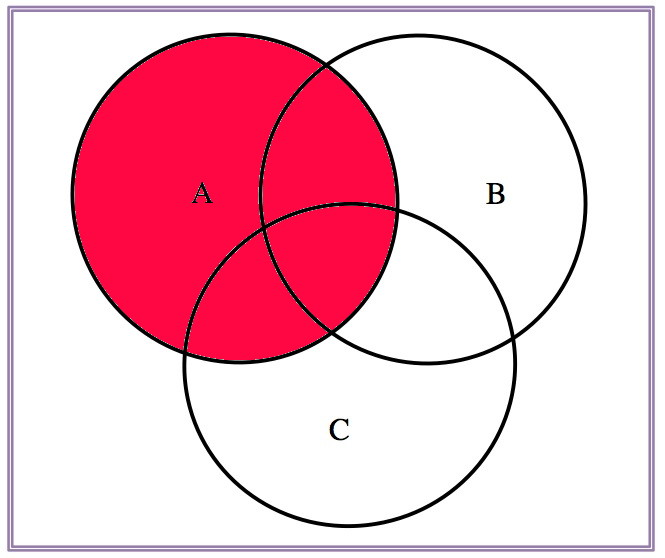
\includegraphics[width=\textwidth,height=4cm]{Images/proba1dibujos/distr11.jpg} & 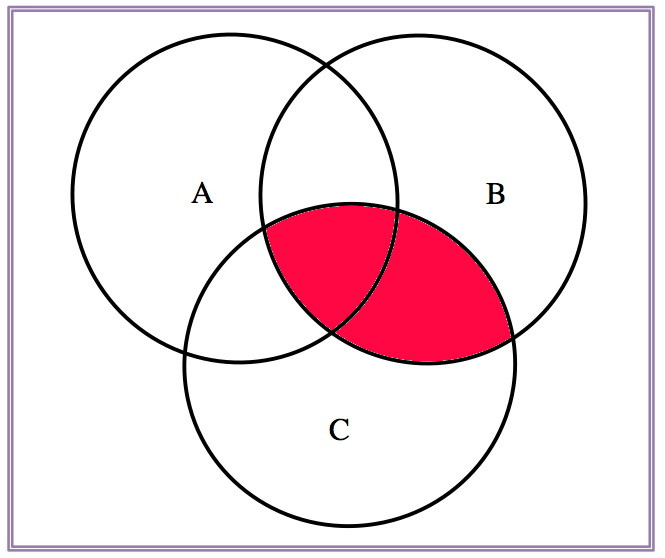
\includegraphics[width=\textwidth,height=4cm]{Images/proba1dibujos/distr12.jpg} & 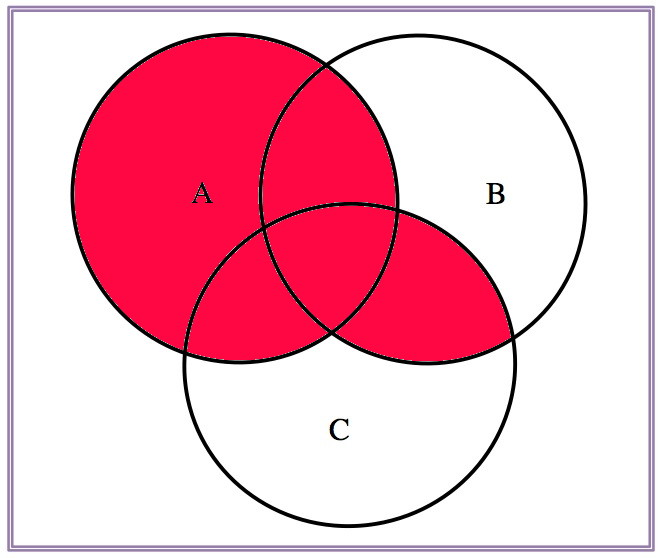
\includegraphics[width=\textwidth,height=4cm]{Images/proba1dibujos/distr13.jpg}\tabularnewline
\bottomrule
\end{longtable}

\begin{longtable}[]{@{}ccc@{}}
\toprule
\(A\cup B\) & \(A\cup C\) & \((A\cup B)\cap (A\cup C)\)\tabularnewline
\midrule
\endhead
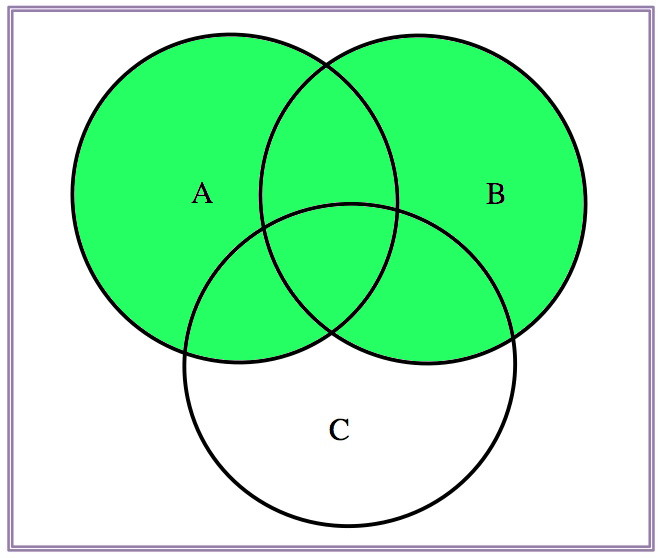
\includegraphics[width=\textwidth,height=4cm]{Images/proba1dibujos/distr21.jpg} & 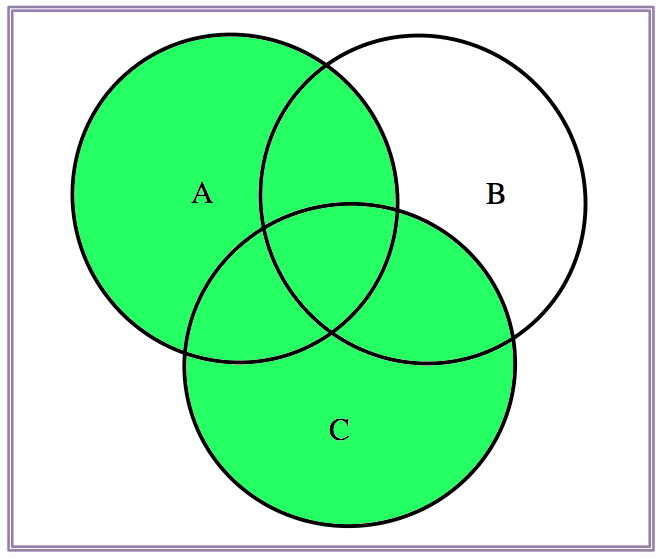
\includegraphics[width=\textwidth,height=4cm]{Images/proba1dibujos/distr22.jpg} & 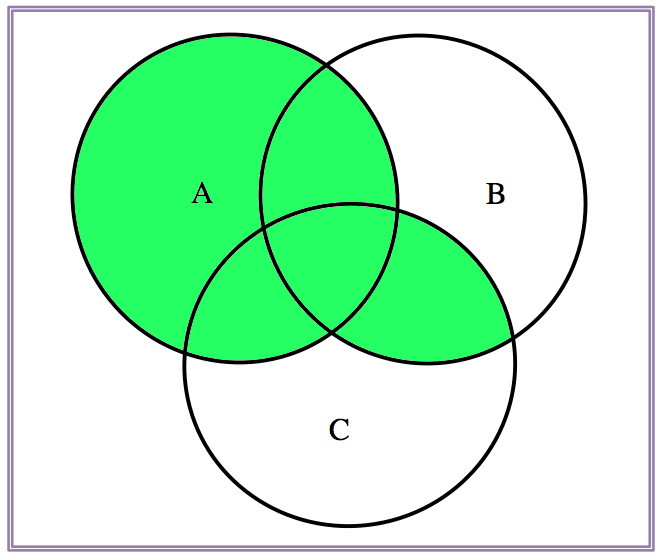
\includegraphics[width=\textwidth,height=4cm]{Images/proba1dibujos/distr23.jpg}\tabularnewline
\bottomrule
\end{longtable}

 Complementario del complementario
\[(A^c)^c=A\]

\begin{longtable}[]{@{}ccc@{}}
\toprule
\(A\) & \(A^c\) & \((A^c)^c\)\tabularnewline
\midrule
\endhead
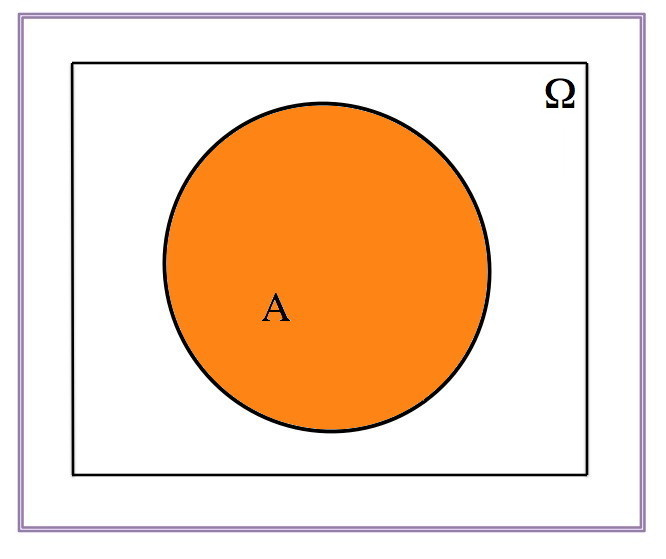
\includegraphics[width=\textwidth,height=4cm]{Images/proba1dibujos/dd2.jpg} & 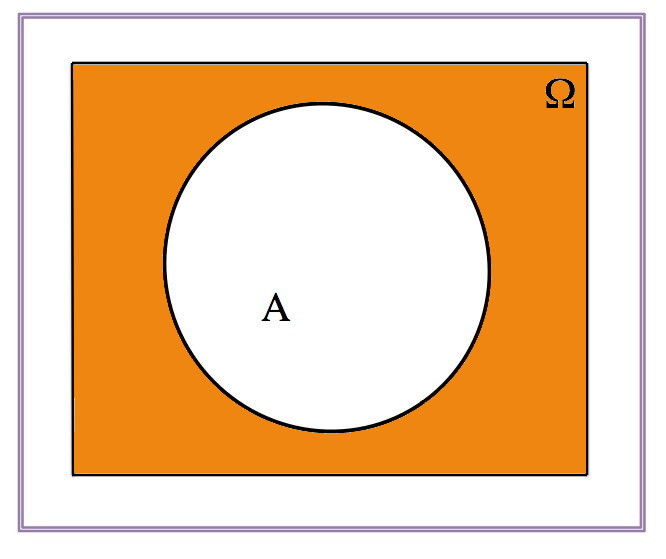
\includegraphics[width=\textwidth,height=4cm]{Images/proba1dibujos/dd1.jpg} & 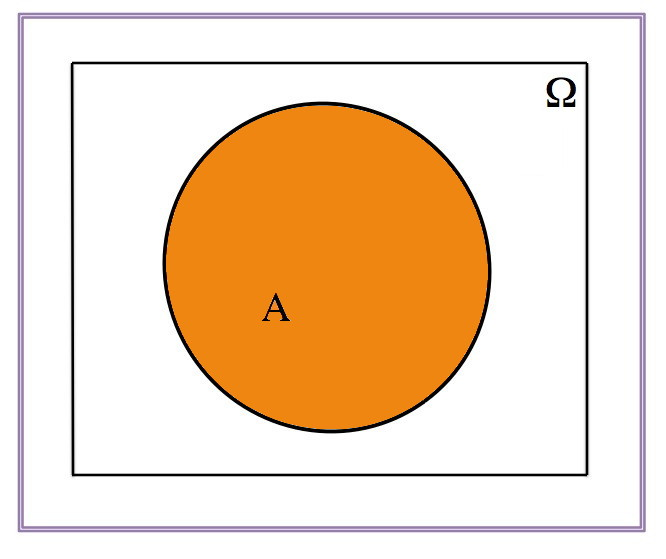
\includegraphics[width=\textwidth,height=4cm]{Images/proba1dibujos/dd3.jpg}\tabularnewline
\bottomrule
\end{longtable}

\textbf{Leyes de De Morgan}

\[(A\cup B)^c=A^c\cap B^c\]

\begin{longtable}[]{@{}cc@{}}
\toprule
\(A\cup B\) & \((A\cup B)^c\)\tabularnewline
\midrule
\endhead
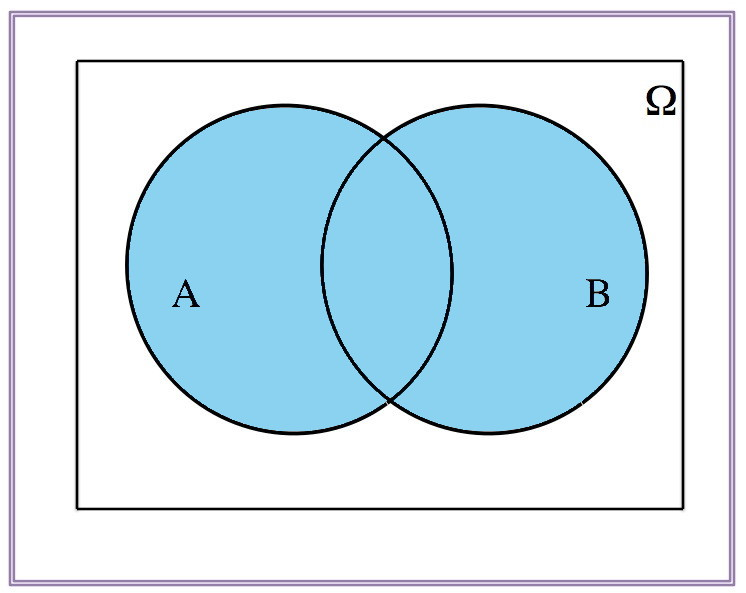
\includegraphics[width=\textwidth,height=6cm]{Images/proba1dibujos/demorgan6.jpg} & 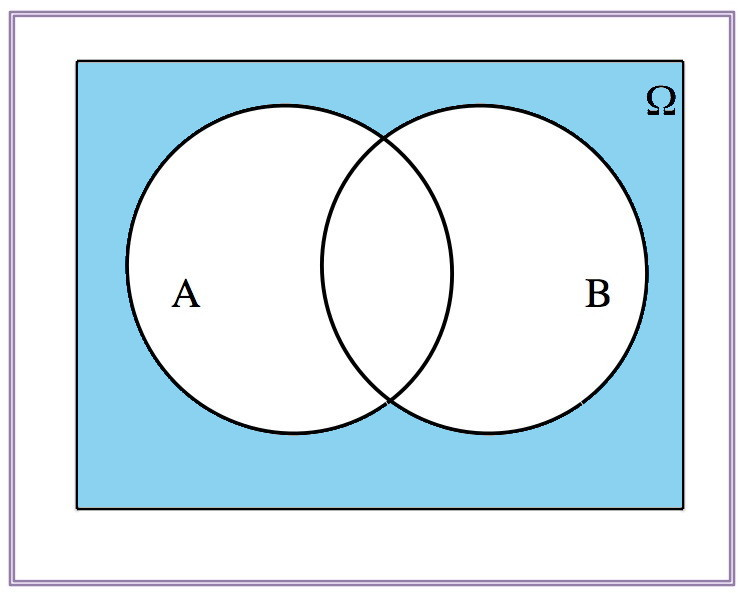
\includegraphics[width=\textwidth,height=6cm]{Images/proba1dibujos/demorgan7.jpg}\tabularnewline
\bottomrule
\end{longtable}

\begin{longtable}[]{@{}ccc@{}}
\toprule
\(A^c\) & \(B^c\) & \(A^c\cap B^c\)\tabularnewline
\midrule
\endhead
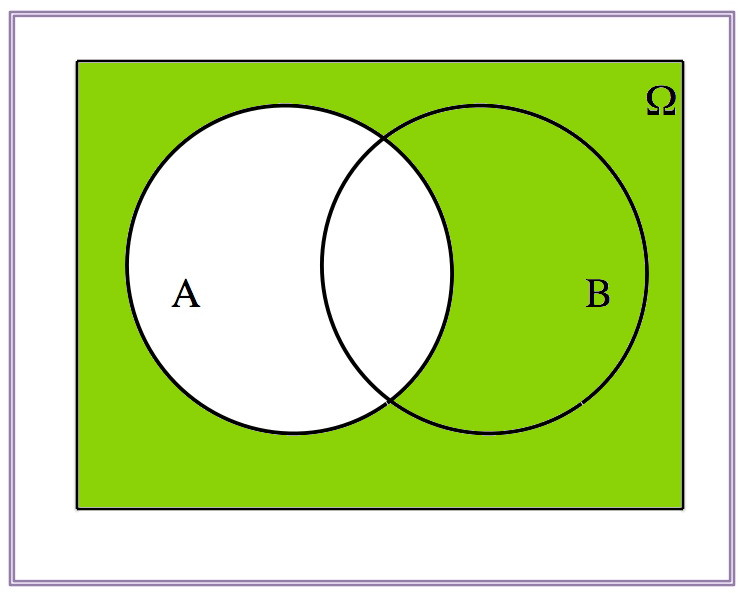
\includegraphics[width=\textwidth,height=4cm]{Images/proba1dibujos/demorgan8.jpg} & 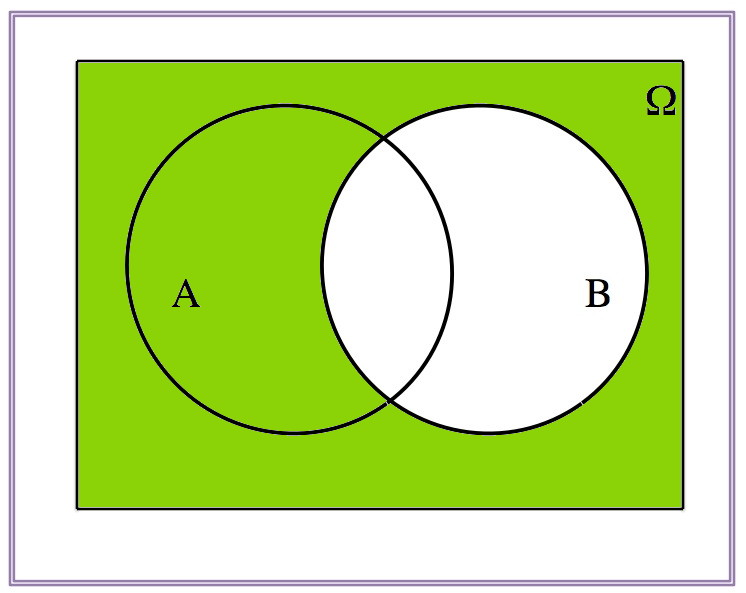
\includegraphics[width=\textwidth,height=4cm]{Images/proba1dibujos/demorgan9.jpg} & 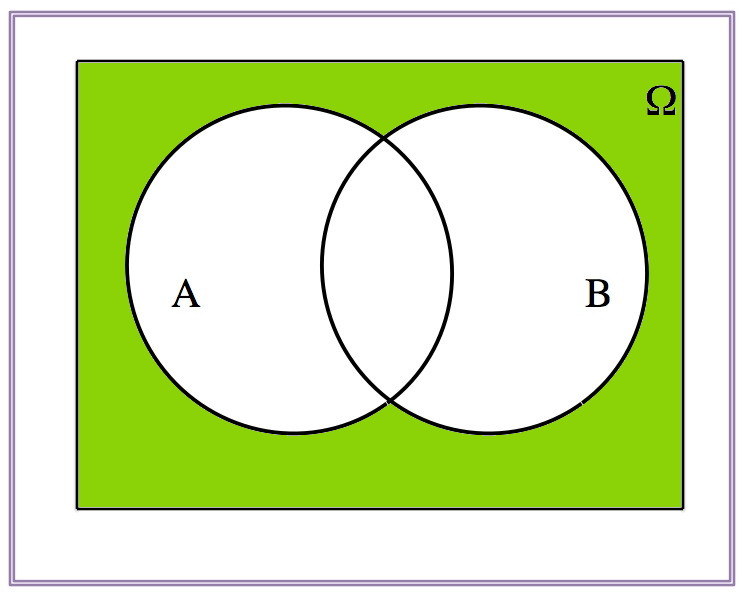
\includegraphics[width=\textwidth,height=4cm]{Images/proba1dibujos/demorgan10.jpg}\tabularnewline
\bottomrule
\end{longtable}

\textbf{Leyes de De Morgan}

\[(A\cap B)^c=A^c\cup B^c\]

\begin{longtable}[]{@{}cc@{}}
\toprule
\(A\cap B\) & \((A\cap B)^c\)\tabularnewline
\midrule
\endhead
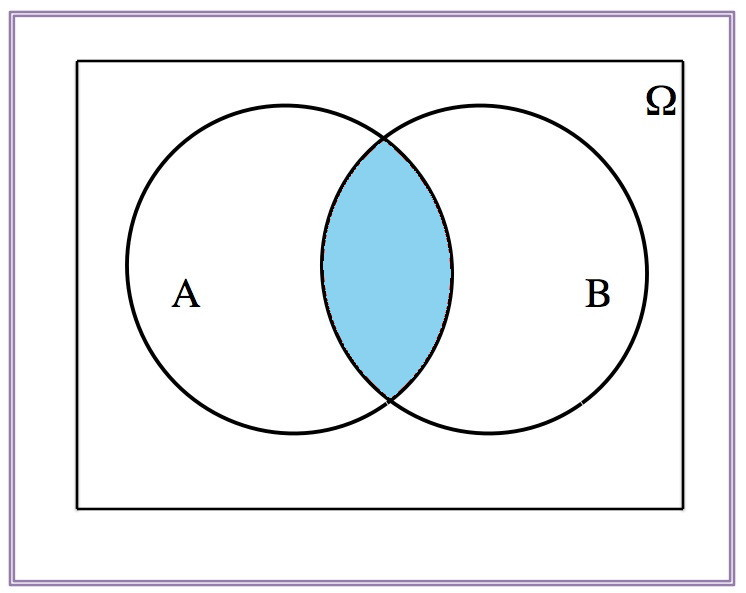
\includegraphics[width=\textwidth,height=6cm]{Images/proba1dibujos/demorgan1.jpg} & 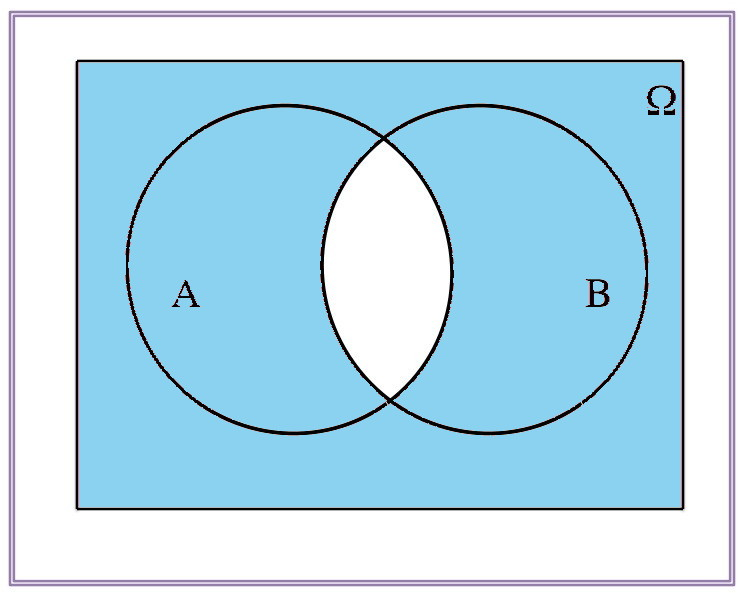
\includegraphics[width=\textwidth,height=6cm]{Images/proba1dibujos/demorgan2.jpg}\tabularnewline
\bottomrule
\end{longtable}

\begin{longtable}[]{@{}ccc@{}}
\toprule
\(A^c\) & \(B^c\) & \(A^c\cup B^c\)\tabularnewline
\midrule
\endhead
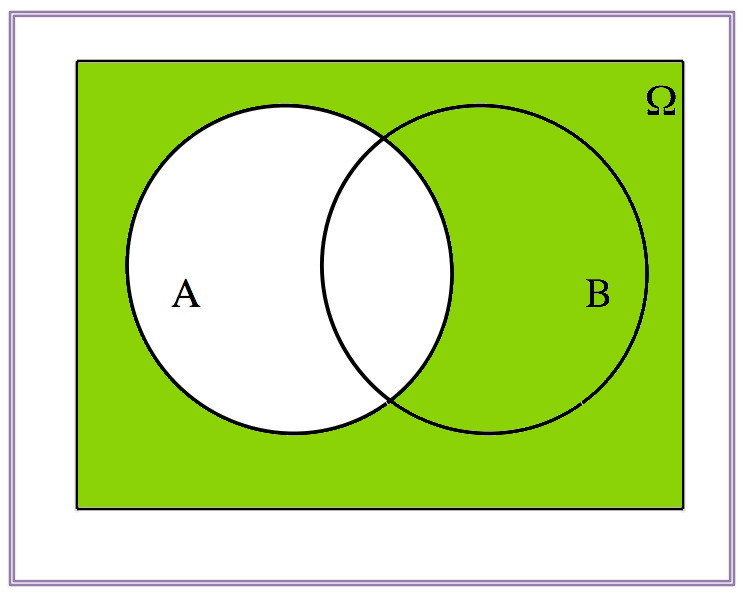
\includegraphics[width=\textwidth,height=4cm]{Images/proba1dibujos/demorgan3.jpg} & 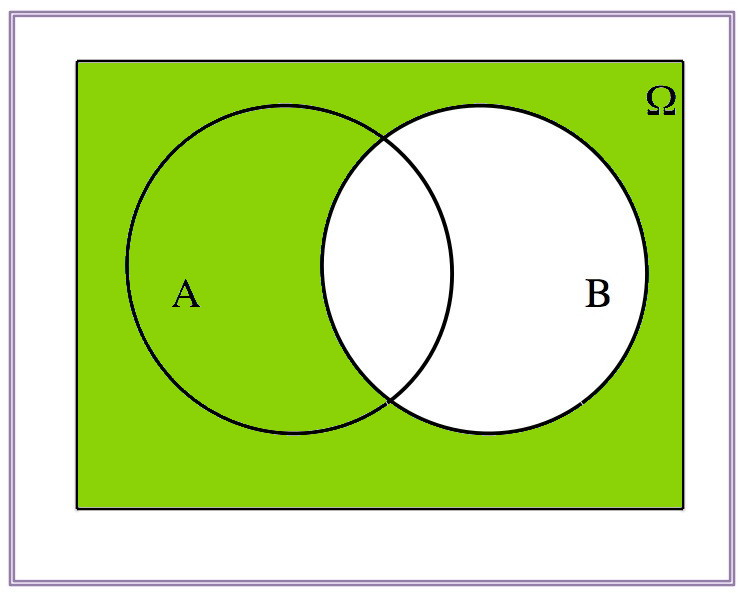
\includegraphics[width=\textwidth,height=4cm]{Images/proba1dibujos/demorgan5.jpg} & 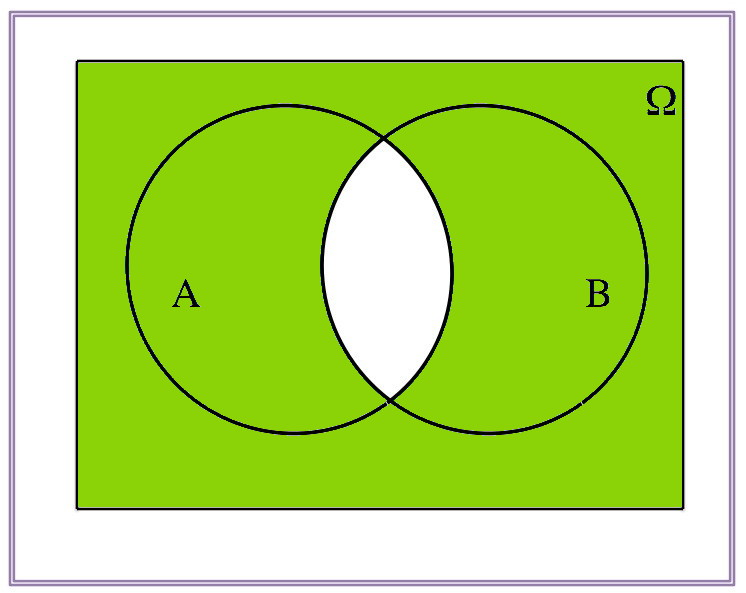
\includegraphics[width=\textwidth,height=4cm]{Images/proba1dibujos/demorgan4.jpg}\tabularnewline
\bottomrule
\end{longtable}

\hypertarget{definiciuxf3n-de-probabilidad}{%
\subsection{Definición de probabilidad}\label{definiciuxf3n-de-probabilidad}}

La probabilidad de un suceso es una puntuación (\emph{score}) numérico entre 0 y 1 que mide la verosimilitud de que este evento se produzca.

Esta verosimilitud puede estar justificada por:

\begin{itemize}
\tightlist
\item
  Estimación personal
\item
  Estimación de expertos
\item
  La frecuencia con la que se da
\item
  Cálculo formal
\end{itemize}

Sea \(\Omega\) el espacio muestral de un experimento aleatorio.
Supongamos que el número de posibles resultados, por el momento, es finito.

Una probabilidad sobre \(\Omega\) es una aplicación \(P:\mathcal{P}(\Omega)\to [0,1]\) con las siguientes propiedades:

\begin{enumerate}
\def\labelenumi{\arabic{enumi}.}
\tightlist
\item
  \(0\leq P(A)\leq 1\), para todo suceso \(A\).
\item
  \(P(\Omega)=1\).
\item
  Si \(\{A_1,A_2,\ldots,A_n\}\) son sucesos disjuntos dos a dos, entonces
\end{enumerate}

\[
P(A_1\cup A_2\cup \cdots \cup A_n)=P(A_1)+P(A_2)+\cdots +P(A_n).
\]

Si \(a\in \Omega\) es un suceso elemental cometeremos el abuso de notación de poner \(P(a)\) en lugar de \(P(\{a\})\).

\textbf{Ejemplo: grupos sangíneos}

En la página de la \href{http://www.donasang.org/que-es-la-sang/es_frequencies-dels-diferents-grups.html}{Fundación Banco de Sangre y Tejidos de las Islas Baleares} podemos encontrar información sobre los porcentajes de tipos de sangre de los donantes de las Islas Baleares:

\[A: 46\%;\ B: 7.5\%;\ AB: 3.5\%;\ O: 43\%.\]

¿Cuál es la probabilidad de que un balear donante de sangre no sea del tipo O?

\textbf{Experimento aleatorio:} tipo de sangre de un paciente humano

\[\Omega=\{\mbox{A,B,AB,O}\}.\]

\textbf{Probabilidad} de un suceso: se asimila al porcentaje observado de individuos

\textbf{Suceso:} \(\{\mbox{O}\}^c=\{\mbox{A,B,AB}\}\)

\[P(\{\mbox{O}\}^c)\!=\!P(\{\mbox{A,B,AB}\})\!=\!
P(\mbox{A})+P (\mbox{B})+P(\mbox{AB})\!=\!0.57.\]

\hypertarget{propiedades-1}{%
\subsection{Propiedades}\label{propiedades-1}}

\textbf{Propiedades básicas de la probabilidad}

\begin{itemize}
\item
  \(P(\emptyset)=0\).
\item
  \(P(A-B)=P(A)-P(A\cap B)\) porque \(P(A)=P(A-B)+P(A\cap B)\).
\end{itemize}

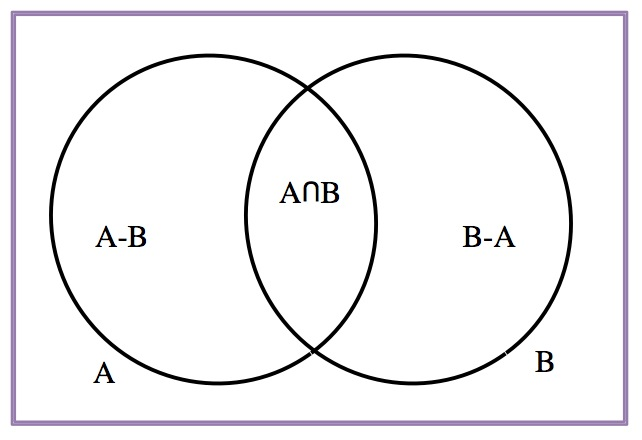
\includegraphics[width=\textwidth,height=2.08333in]{Images/proba1dibujos/A-B.jpg}

\begin{itemize}
\item
  Si \(B\subseteq A\), entonces \(0\leq P(B)\leq P(A)\).
\item
  \(P(A^c)=1-P(A)\).
\item
  \(P(A\cup B)=P(A)+P(B)-P(A\cap B)\) porque
\end{itemize}

\begin{eqnarray*}
P(A)+P(B)-P(A\cap B) &=& P(A-B)+P(A\cap B)+\\
 & & P(B-A)+ P(A\cap  B)-P(A\cap  B)\\
&=& P(A-B)+P(A\cap B)+ P(B-A) \\
&=& P(A\cup B).
\end{eqnarray*}

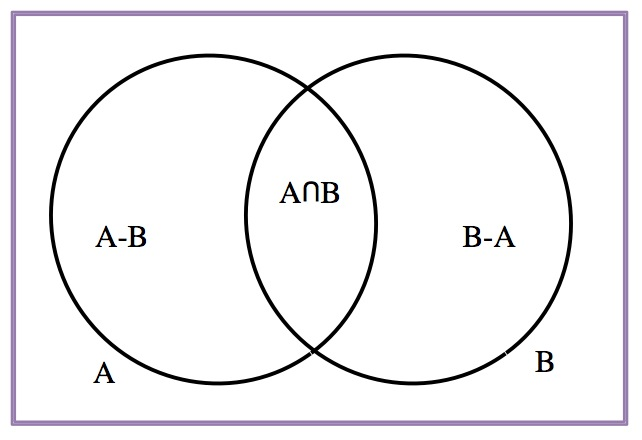
\includegraphics[width=\textwidth,height=2.08333in]{Images/proba1dibujos/A-B.jpg}

\begin{itemize}
\tightlist
\item
  \begin{eqnarray*}
  P(A\cup B\cup C)&=&P(A)+P(B)+P(C)  \\ &&-P(A\cap B)-P(A\cap C)-P(B\cap C)  +P(A\cap B\cap C).
  \end{eqnarray*}
\end{itemize}

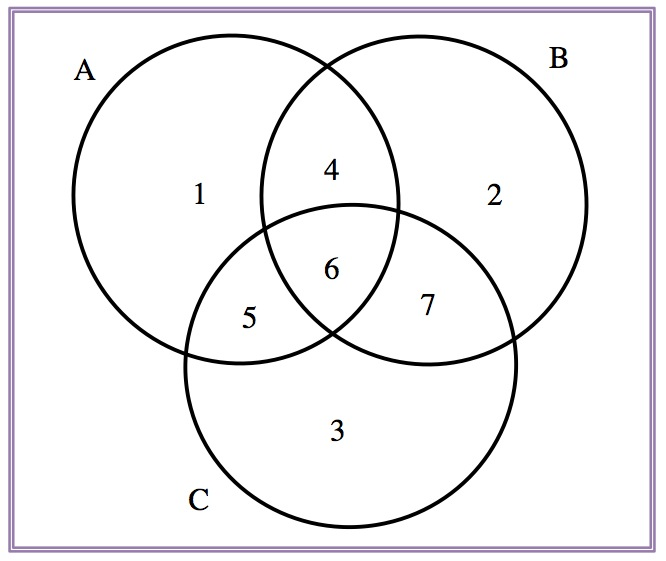
\includegraphics[width=\textwidth,height=2.08333in]{Images/proba1dibujos/tresconjunts.jpg}

\[P(A\cup B\cup C)=P(1)+P(2)+P(3)+P(4)+P(5)+P(6)+P(7).\]

\begin{itemize}
\item
  Si \(A=\{a_1,a_2,\ldots,a_k\}\), entonces
  \[
  P(A)=P(a_1)+P(a_2)+\cdots+P(a_k).
  \]
\item
  Si todos los sucesos elementales tienen la misma probabilidad,
  \[
  P(A)=\frac{|A|}{|\Omega|}\Big(=\frac{\mbox{casos favorables}}{\mbox{casos posibles}}\Big).
  \]
\end{itemize}

\textbf{Ejemplo: Frecuencia de vocales}

Los porcentajes de vocales de un determinado idioma (de alfabeto latino) según la \href{https://es.wikipedia.org/wiki/Frecuencia_de_aparici\%C3\%B3n_de_letras}{Wikipedia} son:

\[A: 18.7\%;\ E: 26.1\%;\ I: 25.7\%;\ O: 24.4\%;\  U: 5.1\%.\]

¿Cuál es la probabilidad que una vocal escogida al azar de este idioma sea una E o una O?

El espacio muestral del experimento es \(\Omega=\{A,E,I,O,U\}\).

El suceso que deseamos analizar es \(\{E,0\}\).

Y su probabilidad es

\[P(\{E,O\})=P(E)+P(O)=0.261+0.244=0.505.\]

\textbf{Ejemplo: Consumo de drogas}

Segun un árticulo de \href{https://elpais.com/politica/2019/01/02/actualidad/1546426491_623324.html}{El País}, en un control especial de la policía el \(0.1\%\) de todos los conductores analizados en un control de tráfico dan positivo en un el test en cocaína, y el \(1\%\) da positivo en cannabis. Un \(1.05\%\) da positivo en alguno de los dos test.

¿Cuál es la probabilidad que un individuo analizado en el control de drogas escogido al azar no de positivo en ninguno de lo dos test?

Los sucesos elementales del enunciado del problema son:

\begin{itemize}
\tightlist
\item
  \(A\): dar positivo en cocaína; \(P(A)=0.001\).
\item
  \(B\): dar positivo en cannabis; \(P(B)=0.01\).
\end{itemize}

En este caso nos interesa estudiar los sucesos:

\begin{itemize}
\tightlist
\item
  \(A\cup B\): dar positivo en alguno de los dos test; \(P(A\cup B)=0.0105\).
\item
  \((A\cup B)^c\): no dar positivo en ninguno de los test,
\end{itemize}

de donde, por tanto:
\[P((A\cup B)^c)=1-P(A\cup B)=1-0.0105=0.9895.\]

\textbf{Ejemplo}

En un control especial de la policía el \(0.1\%\) de todos los conductores analizados en un control de tráfico dan positivo en un el test en cocaína, y el \(1\%\) da positivo en cannabis. Un \(1.05\%\) da positivo en alguno de los dos test.

¿Cuál es la probabilidad que un analizado al azar de positivo en los dos test en cocaína y cannabis?

Los sucesos elementales son:

\begin{itemize}
\tightlist
\item
  \(A\): dar positivo en cocaína; \(P(A)=0.001\).
\item
  \(B\): dar positivo en cannabis; \(P(B)=0.01\).
\end{itemize}

En este caso nos interesa estudiar los sucesos:

\begin{itemize}
\tightlist
\item
  \(A\cup B\): dar positivo en algún de los dos test; \(P(A\cup B)=0.0105\).
\item
  \(A\cap B\): dar positivo en los dos test,
\end{itemize}

de donde, por tanto:

\[\begin{array}{rl}
{P(A\cap B)} &{=P(A)+P(B)-P(A\cup B)}\\ &{=0.001+0.01-0.0105=0.0005}.
\end{array}\]

¿Cuál es la probabilidad de que un conductor analizado de positivo en cocaína pero no en cannabis?

Los sucesos elementales son:

\begin{itemize}
\tightlist
\item
  \(A\): dar positivo en cocaína; \(P(A)=0.001\).
\item
  \(B\): dar positivo en cannabis; \(P(B)=0.01\).
\end{itemize}

En este caso nos interesa estudiar los sucesos:

\begin{itemize}
\tightlist
\item
  \(A\cap B\): dar positivo en los dos test; \(P(A\cap B)=0.0005\).
\item
  \(B-A\): dar positivo en cocaína pero no en cannabis,
\end{itemize}

de donde, por tanto:

\[P(B-A) =P(B)-P(A\cap B) =0.01-0.0005=0.0095.\]

\hypertarget{probabilidad-condicionada}{%
\section{Probabilidad condicionada}\label{probabilidad-condicionada}}

 \textbf{Probabilidad condicionada}: Dados dos sucesos \(A\) y \(B\), con \(P(A)>0\), la probabilidad \(P(B|A)\) de \(B\) condicionado a \(A\) es la probabilidad

\begin{itemize}
\tightlist
\item
  de que suceda \(B\) suponiendo que pasa \(A\),
\item
  de que si pasa \(A\), entonces suceda \(B\),
\item
  de que un resultado de \(A\) también pertenezca a \(B\).
\end{itemize}

Se calcula a través de la definición:

\[
P(B|A)=\frac{P(A\cap B)}{P(A)}.
\]

\textbf{Ejemplo: frecuencia género y gafas}

En una clase de 20 hombres y 30 mujeres, 15 hombres y 18 mujeres llevan gafas. Contestemos las siguientes preguntas:

\begin{itemize}
\tightlist
\item
  ¿Cuál es la probabilidad de que un alumno lleve gafas?
\end{itemize}

\[
\frac{33}{50}.
\]

\begin{itemize}
\tightlist
\item
  ¿Cuál es la probabilidad de que un alumno sea mujer y lleve gafas?
\end{itemize}

\[
\frac{18}{50}.
\]

\begin{itemize}
\tightlist
\item
  ¿Cuál es la probabilidad de que un chica lleve gafas?
\end{itemize}

\[
\frac{18}{30}=\frac{18/50}{30/50}=\frac{P(\mbox{mujer  y gafas})}{P(\mbox{mujer})}.
\]

\begin{itemize}
\tightlist
\item
  Si escogemos un estudiante al azar ¿Cuál es la probabilidad que si es mujer, entonces lleve gafas?
\end{itemize}

\[
\frac{18}{30}.
\]

\begin{itemize}
\tightlist
\item
  ¿Cuál es la probabilidad de que un alumno que lleve gafas sea mujer?
\end{itemize}

\[
\frac{18}{33}=\frac{18/50}{33/50}=\frac{P(\mbox{mujer y gafas})}{P(\mbox{gafas})}.
\]

\begin{itemize}
\tightlist
\item
  Si escogemos un estudiante al azar ¿Cuál es la probabilidad de que si lleva gafas, entonces sea mujer?
  \[
  \frac{18}{33}.
  \]
\end{itemize}

\hypertarget{atenciuxf3n}{%
\subsection{¡Atención!}\label{atenciuxf3n}}

Hay que distinguir bien entre

\begin{itemize}
\item
  \(P(A\cap B)\): probabilidad de \(A\) \(\color{red}{\text{y}}\) \(B\), \emph{Probabilidad de que sea mujer y lleve gafas}.
\item
  \(P(A|B)\): probabilidad de que \(\color{red}{\text{si}}\) pasa \(B\), \(\color{red}{\text{entonces}}\) pase \(A\), \emph{Probabilidad de que, si es mujer, lleve gafas}.
\end{itemize}

Cuando utilizamos probabilidad condicional \(P(A|B)\) estamos restringiendo el espacio muestral a \(B\).

\hypertarget{propiedades-2}{%
\subsection{Propiedades}\label{propiedades-2}}

La probabilidad condicionada es una probabilidad

\textbf{Proposición}

Sea \(A\subseteq \Omega\) un suceso tal que \(P(A)>0\), entonces

\[
\begin{array}{rccl}
P(-|A):& \mathcal{P}(\Omega) & \to & [0,1]\\
&B & \mapsto & P(B|A).
\end{array}
\]
satisface las propiedades de las probabilidades, como por ejemplo:

\[
\begin{array}{l}
P(B^c|A)=1-P(B|A),\\
P(B_1\cup B_2|A)=P(B_1|A)+P(B_2|A)-P(B_1\cap B_2|A).
\end{array}
\]

\textbf{Ejercicio}

Escribid el resto de propiedades que cumpliría una probabilidad condicionada al evento \(A\).

\textbf{Ejemplo: Hipertensos}

Un 15\% de los adultos son hipertensos, un 25\% de los adultos creen que son hipertensos, y un 9\% de los adultos son hipertensos y creen que lo son.

\begin{itemize}
\tightlist
\item
  ¿Si un adulto cree que es hipertenso, ¿cuál es la probabilidad que lo sea?
\item
  ¿Si un adulto es hipertenso, ¿cuál es la probabilidad que crea que lo es?
\end{itemize}

Sean los sucesos

\begin{itemize}
\tightlist
\item
  \(A\): ser hipertenso; \(P(A)=0.15\).
\item
  \(B\): creer ser hipertenso; \(P(B)=0.25\),
\end{itemize}

entonces podemos definir el suceso:

\begin{itemize}
\tightlist
\item
  \(A\cap B\): ser hipertenso y creerlo; \(P(A\cap B)=0.09\),
\end{itemize}

de donde, la probabilidad condicionada de ser hipertenso creyéndonos que lo somos es:

\[P(A|B)=\dfrac{P(A\cap B)}{P(B)}=\dfrac{0.09}{0.25}=0.36.\]

¿Si un adulto es hipertenso, ¿cuál es la probabilidad que crea que lo es?

¿Si un adulto es hipertenso, ¿cuál es la probabilidad que crea que lo es?

Si tenemos los sucesos:

\begin{itemize}
\tightlist
\item
  \(A\): ser hipertenso,
\item
  \(B\): creer ser hipertenso,
\end{itemize}

entonces buscamos la probabilidad \(P(B|A)\):

\[
\begin{array}{rl}
P(B|A) & =\dfrac{P(A\cap B)}{P(A)}=\dfrac{0.09}{0.15}=
0.6.
\end{array}
\]

\textbf{Ejemplo: dígitos de control}

Un dígito de control de error toma el valor 0 en el 99\% de los casos en que hay un error. Si la probabilidad de error en un mensaje es del \(0.5\%\). ¿cuál es la probabilidad de que el mensaje sea erróneo y el código de error tenga valor 0?

\begin{itemize}
\tightlist
\item
  \(B\): mensaje con error; \(P(B)=0.005\),
\item
  \(A\): código de error vale 0,
\item
  \(P(A|B)=0.99\),
\end{itemize}

entonces:
\[P(A\cap B)=P(B)\cdot P(A|B)=0.005\cdot 0.99=0.00495.\]

\textbf{Ejemplo: SPAM}

Un 50\% de correos recibidos en un servidor llevan adjuntos y un 65\% son publicidad no deseada (SPAM). Sólo un 15\% de estos correos no llevan adjuntos y no son SPAM.

\begin{itemize}
\tightlist
\item
  ¿Cuál es la probabilidad que un correo lleve adjunto si es SPAM?
\item
  ¿Cuál es la probabilidad que un correo \textbf{no} tenga adjuntos si \textbf{no} es SPAM?
\item
  ¿Cuál es la probabilidad de que un correo no lleve adjuntos si no es SPAM?
\end{itemize}

¿Cuál es la probabilidad que un correo lleve adjunto si es SPAM?

\begin{itemize}
\tightlist
\item
  \(A\): llevar adjuntos, \(P(A)=0.5\),
\item
  \(S\): SPAM, \(P(S)=0.65\),
\item
  \(A^c\cap S^c=(A\cup S)^c\): no llevar adjunto y no ser SPAM, \(P((A\cup S)^c)=0.15\).
\end{itemize}

\[P(A|S)=\dfrac{P(A\cap S)}{P(S)}=?\]

\begin{itemize}
\item
  \(P(A)=0.5, P(S)=0.65, P(A^c\cap S^c)=P((A\cup S)^c)=0.15\),
\item
  \(P(A\cup S)=1-P((A\cup S)^c)=0.85\),
\item
  \(P(A\cap S)=P(A)+P(S)-P(A\cup S)=0.3\),
\end{itemize}

\[P(A|S)=\dfrac{P(A\cap S)}{P(S)}=\dfrac{0.3}{0.65}\approx 0.46.\]

¿Cuál es la probabilidad de que un correo no lleve adjuntos si no es SPAM?

\[P(A)=0.5, P(S)=0.65, P(A^c\cap S^c)=P((A\cup S)^c)=0.15.\]

\[P(A^c|S^c)=\dfrac{P(A^c\cap S^c)}{P(S^c)}=\dfrac{P(A^c\cap S^c)}{1-P(S)}=\dfrac{0.15}{0.35}\approx 0.43.\]

\hypertarget{teorema-de-la-probabilidad-total}{%
\subsection{Teorema de la probabilidad total}\label{teorema-de-la-probabilidad-total}}

\textbf{Teorema de la probabilidad total}

Dados dos sucesos \(A\) y \(B\) se tiene que

\[
\begin{array}{rl}
P(B)&= P(B\cap A) +P(B\cap A^c)\\
& =P(A)\cdot P(B|A)+ P(A^c)\cdot P(B|A^c).
\end{array}
\]

\textbf{Partición del espacio espacio muestral}

Los sucesos \(A_1,A_2,\ldots, A_n\) son una \textbf{partición} del espacio muestral \(\Omega\) de un determinado experimento aleatorio, si cumplen las condiciones siguientes:

\begin{enumerate}
\def\labelenumi{\arabic{enumi}.}
\tightlist
\item
  \(A_1\cup A_2\cup\ldots\cup A_n=\Omega\),
\item
  \(A_1,A_2,\ldots,A_n\) son incompatibles dos a dos (\(A_i\cap A_j=\emptyset\)).
\end{enumerate}

\textbf{Teorema de la probabilidad total (generalización)}
Sea \(A_1,A_2,\ldots,A_n\) una partición de \(\Omega\). Sea \(B\) un suceso cualquiera. Entonces

\[
\begin{array}{rl}
P(B)&= P(B\cap A_1)+\cdots +P(B\cap A_n)\\
& =P(A_1)\cdot P(B|A_1)+\ldots+P(A_n)\cdot P(B|A_n).
\end{array}
\]

\textbf{Ejemplo: Dígito de control de error}

Un dígito de control de error toma el valor 0 en un \(99\%\) de los casos en que hay un error y en un \(5\%\) de los mensajes sin error.
La probabilidad de error en un mensaje es del \(0.5\%\).

¿Cuál es la probabilidad de que un mensaje escogido al azar tenga el dígito de control a 0?

Sean los sucesos del enunciado:

\begin{itemize}
\tightlist
\item
  \(B\): mensaje con error; \(P(B)=0.005\),
\item
  \(A\): código de error vale 0,
\end{itemize}

entonces obtenemos las probabilidades a partir del enunciado:

\begin{itemize}
\tightlist
\item
  \(P(A|B)=0.99\),
\item
  \(P(A|B^c)= 0.05\),
\end{itemize}

y por tanto,

\[
\begin{array}{rl}
P(A) & =P(B)\cdot P(A|B)+P(B^c)\cdot P(A|B^c)\\ &
=0.005\cdot 0.99+0.995\cdot 0.05=0.0547.\end{array}
\]

\hypertarget{clasificaciuxf3n-o-diagnuxf3sticos}{%
\subsection{Clasificación o Diagnósticos}\label{clasificaciuxf3n-o-diagnuxf3sticos}}

Consideremos alguna de las siguientes situaciones:

\begin{itemize}
\tightlist
\item
  Un algoritmo detecta si una transacción con tarjeta de crédito es fraude o no.
\item
  Un algoritmo detecta si tiene o no que mostrar un anuncio en una web.
\item
  Un prueba de embarazo.
\item
  Una prueba médica para una enfermedad concreta.
\end{itemize}

Nos ceñiremos a la casuística más elemental el algoritmo de clasificación o la diagnosis solo da dos resultado \textbf{Positivo} (sí tienes la enfermedad, sí es un fraude) o \textbf{Negativo} (en caso contrario).

En todas estas situaciones podemos calcular lo que se llama \textbf{matriz de confusión} que representa todas las situaciones posibles. En el caso de estudiar una condición de tipo binario,

\begin{longtable}[]{@{}lcc@{}}
\toprule
& El Test da Positivo & El Test da Negativo\tabularnewline
\midrule
\endhead
Condición Positiva & Correcto & Error\tabularnewline
Condición Negativa & Error & Correcto\tabularnewline
\bottomrule
\end{longtable}

En general los modelos y algoritmos de clasificación suelen aportar puntuaciones (\emph{scores}) que determinan el grado de pertenencia a una clase, o que miden si dos objetos están en la misma clase.

Así el resultado del clasificador o del diagnóstico puede ser:

\begin{itemize}
\tightlist
\item
  \textbf{un número real}, en cuyo caso debe clasificador entre cada clase debe determinarse por un valor umbral (\emph{threshold}) por ejemplo para determinar si una persona está estresado podemos dar un \emph{scores} entre 0 y 1 (1 máximo estrés 0 estrés nulo),
\item
  \textbf{un resultado discreto} que indica directamente una de las clases (esto es necesario si es un algoritmo que debe decidir qué hacer con el objeto.
\end{itemize}

 \textbf{Positivos y Negativos en Clasificación}
Consideremos un problema de predicción de clases binario, en la que los resultados se etiquetan positivos (P) o negativos (N). Hay cuatro posibles resultados a partir de un clasificador binario como el propuesto.

\begin{itemize}
\tightlist
\item
  Si el resultado de una exploración es P y el valor dado es también P, entonces se conoce como un Verdadero Positivo (VP).
\item
  Sin embargo si el valor real es N entonces se conoce como un Falso Positivo (FP).
\item
  De igual modo, tenemos un Verdadero Negativo (VN) cuando tanto la exploración como el valor dado son N.
\item
  Un Falso Negativo (FN) cuando el resultado de la predicción es N pero el valor real es P.
\end{itemize}

Un ejemplo aproximado de un problema real es el siguiente: consideremos una prueba diagnóstica que persiga determinar si una persona tiene una cierta enfermedad.

\begin{itemize}
\tightlist
\item
  Un falso positivo en este caso ocurre cuando la prueba predice que el resultado es positivo, cuando la persona no tiene realmente la enfermedad.
\item
  Un falso negativo, por el contrario, ocurre cuando el resultado de la prueba es negativo, sugiriendo que no tiene la enfermedad cuando realmente sí la tiene.
\end{itemize}

En un diagnósticos de una cierta condición (por ejemplo, test embarazo, test de enfermedad), tenemos dos tipos de sucesos:

\begin{itemize}
\tightlist
\item
  \(T\): el test da positivo,
\item
  \(M\): el sujeto satisface la condición,
\item
  \textbf{Falsos positivos} \(T\cap M^c\): El test da positivo, pero la condición no se da,
\item
  \textbf{Coeficiente de falsos positivos} \(P(T|M^c)\),
\item
  \textbf{Falsos negativos} \(T^c\cap M\): El test da negativo, pero la condición sí que se da,
\item
  \textbf{Coeficiente de falsos negativos}: \(P(T^c|M)\).
\end{itemize}

\textbf{Ejemplo: Prueba médica}

Un test diseñado para diagnosticar una determinada enfermedad tiene un coeficiente de falsos negativos de 0.06, y un coeficiente de falsos positivos de 0.04. En un estudio masivo se observa que un 15\% de la población da positivo al test.

¿Cuál es la probabilidad que una persona escogida aleatoriamente tenga esta enfermedad?

Los datos del problema son:

\begin{itemize}
\tightlist
\item
  \(T\): dar positivo al test; \(P(T)=0.15\),
\item
  \(M\): tener la enfermedad,
\item
  \(P(T)=0.15\), \(P(T^c|M)=0.06\), \(P(T|M^c)=0.04\),
\item
  ¿\(P(M)\)?
\end{itemize}

\[
P(T) =P(M)\cdot P(T|M)+P(M^c)\cdot P(T|M^c),
\]

donde

\[
\begin{array}{l}
P(T|M)=1-P(T^c|M)=0.94, \\[1ex]
P(M^c)=1-P(M).
\end{array}
\]

Por lo tanto

\[
\begin{array}{rl}
0.15 & = P(M)\cdot 0.94+(1-P(M))\cdot 0.04\\
 & =0.04+0.9\cdot P(M),\\[1ex]
P(M) & =\dfrac{0.11}{0.9}\approx 0.1222.
\end{array}
\]

\hypertarget{bayes}{%
\section{Bayes}\label{bayes}}

\hypertarget{fuxf3rmula-de-bayes}{%
\subsection{Fórmula de Bayes}\label{fuxf3rmula-de-bayes}}

 \textbf{Teorema de Bayes}

Sean \(A\) y \(B\) dos sucesos. Si \(P(B)>0\), entonces

\begin{eqnarray*}
P(A|B) & = & \frac{P(A)\cdot P(B\big|A)}{P(B)}\\
&=& \frac{P(A)\cdot P(B\big|A)}{P(A)\cdot P(B\big|A)+P(A^c)\cdot P(B\big|A^c)}.
\end{eqnarray*}

\textbf{Ejercicio}

Demostrar el teorema de Bayes utilizando que

\[P(A|B) =\frac{P(A\cap B)}{P(B)}=\cdots\]

 \textbf{Teorema de Bayes generalizado}

Sea \(A_1,A_2,\ldots,A_n\) una partición de \(\Omega\). Sea \(B\) un suceso tal que \(P(B)>0\). entonces(para cualquier \(i=1,2,\ldots,n\)):

\begin{eqnarray*}
P(A_i|B) & =& \dfrac{P(A_i)\cdot P(B|A_i)}{P(B)}\\
& =& \dfrac{P(A_i)\cdot P(B|A_i)}{P(A_1)\cdot P(B|A_1)+\cdots+P(A_n)\cdot P(B|A_n)}.
\end{eqnarray*}

\textbf{Ejercicio}

Demostrar el teorema de Bayes utilizando que

\[P(A_i|B) =\dfrac{P(A_i\cap B)}{P(B)}=\cdots\]

\textbf{Ejemplo: Test VIH}

Un test para detección de VIH da positivo un 99\% de los casos en los que está presente y en un 5\% de los casos en los que el virus está ausente. En una población con un \(0.5\%\) de infectados por VIH:

\begin{itemize}
\tightlist
\item
  ¿Cuál es la probabilidad que un individuo que haya dado positivo en el test esté infectado?
\item
  ¿Cuál es la probabilidad de que un individuo que haya dado \textbf{negativo} en el test \textbf{no} esté infectado?
\end{itemize}

Los sucesos del ejemplo son:

\begin{itemize}
\tightlist
\item
  \(A\): individuo infectado,
\item
  \(B\): el test da positivo.
\end{itemize}

Ahora podemos calcular la probabilidad que un individuo que haya dado positivo en el test esté infectado:

\begin{eqnarray*}
P(A|B) & =& \dfrac{P(B|A)\cdot P(A)}{P(B|A)\cdot P(A)+P(B|A^c)\cdot P(A^c)}\\
&=&\dfrac{0.99\cdot 0.005}{0.005\cdot 0.99+0.995\cdot 0.05}=0.09.
\end{eqnarray*}

Para calcular la probabilidad de que un individuo que haya dado \textbf{negativo} en el test \textbf{no} esté infectado hacemos:

\[
\begin{array}{rl} P(A^c|B^c)& =\dfrac{P(B^c|A^c)\cdot P(A^c)}{P(B^c|A)\cdot P(A)+P(B^c|A^c)\cdot P(A^c)}\\ & =\dfrac{0.95\cdot 0.995}{0.01\cdot 0.005+0.95\cdot 0.995}=0.999947.\end{array}
\]

\textbf{Ejercicio: Ventas por internet}

Se ha observado que los cientes de una empresa de ventas por internet son de tres tipos, A, B y C, disjuntos dos a dos. La probabilidad que ser de cualquiera de cada uno de los tipos es \(1/3\), pero la probabilidad de compra de cada tipo es diferente: si es de tipo A compra un 50\% de las veces, si de tipo B, un 75\% de las veces, y de tipo C, un 60\%.

Supongamos que llega un cliente ¿cuál es la probabilidad de que si ha comprado sea del tipo B?

\begin{itemize}
\tightlist
\item
  Los sucesos del ejercicio son \(A\): el cliente es de tipo A, \(B\): el cliente es de tipo B, \(C\): el cliente es de tipo C.
\end{itemize}

\[P(A)=P(B)=P(C)=1/3.\]

Buscamos estudiar el suceso \(E\): el cliente compra, se tiene que:

\[P(E|A)=0.5, P(E|B)=0.75, P(E|C)=0.6.\]

\[P(B|E)\!=\!\dfrac{P(E|B)\cdot P(B)}{P(E|A)\!\cdot\! P(A)\!+\!P(E|B)\!\cdot\! P(B)\!+\!P(E|C)\!\cdot\! P(C)}\!=\!\ldots\]

\textbf{Ejercicio: Detección precoz de abandono de clientes}

Un test de detección precoz de abandono de clientes de una empresa de telefonía da positivo el 97.5\% de las ocasiones en las que, posteriormente, el cliente se da de baja, y un 12\% de las veces en que no se dio de baja. La probabilidad que un cliente escogido al azar se dé de baja es de un 2\%.

\begin{itemize}
\tightlist
\item
  ¿Cuál es la probabilidad que un individuo escogido al azar de positivo en el test?
\item
  ¿Cuál es la probabilidad que un individuo escogido al azar se de de baja y dé positivo en el test?
\item
  ¿Cuál es la probabilidad que un individuo que dé negativo en el test se dé de baja?
\end{itemize}

Definimos los sucesos y datos del ejercicio:

\begin{itemize}
\tightlist
\item
  \(T\): Dar positivo al test,
\item
  \(B\): darse de baja; \(P(B)=0.02\),
\item
  \(P(T|B)=0.975, P(T|B^c)=0.12\).
\end{itemize}

\[P(B)=0.02, P(T|B)=0.975, P(T|B^c)=0.12.\]

¿Cuál es la probabilidad que un individuo escogido al azar de positivo en el test?

\begin{eqnarray*}
P(T) &= & P(B)\cdot P(T|B)+P(B^c)\cdot P(T|B^c)\\
& = &0.02\cdot 0.975+0.98\cdot 0.12=0.1371.
\end{eqnarray*}

¿Cuál es la probabilidad que un individuo escogido al azar se de de baja y dé positivo en el test?

\[P(B\cap T)= P(B)\cdot P(T|B)=0.02\cdot 0.975=0.0195.\]

¿Cuál es la probabilidad que un individuo que dé negativo en el test se dé de baja?

\begin{eqnarray*}
P(B|T^c) & = &\displaystyle \frac{P(B\cap T^c)}{P(T^c)}=
\frac{P(B)-P(B\cap T)}{1-P(T)}\\
& = & \displaystyle
\frac{0.02-0.0195}{1-0.1371}\approx 0.00058.
\end{eqnarray*}

O también se obtiene así
\[
P(B|T^c)=\frac{P(T^c|B)\cdot P(B)}{P(T^c|B)\cdot P(B)+P(T^c|B^c)\cdot P(B^c)},
\]

donde

\begin{eqnarray*}
P(T^c|B)&=&1-P(T|B)=0.025,\\ P(T^c|B^c)&=&1-P(T|B^c)=0.88.
\end{eqnarray*}

\hypertarget{independencia-de-sucesos}{%
\section{Independencia de sucesos}\label{independencia-de-sucesos}}

\hypertarget{sucesos-independientes}{%
\subsection{Sucesos independientes}\label{sucesos-independientes}}

 \textbf{Sucesos Independientes}

Diremos que los sucesos \(A\) y \(B\) son \textbf{independientes} si \(P(A\cap B)=P(A)\cdot P(B)\).

\(A_1,\ldots, A_n\) son sucesos \textbf{independientes} cuando, para toda
subfamilia \(A_{i_1},\ldots,A_{i_k}\),
\[
P(A_{i_1}\cap \cdots\cap A_{i_k})=P(A_{i_1})\cdots P(A_{i_k}).
\]

 \textbf{Proposición:}

Dados dos sucesos \(A\) y \(B\) con \(P(A),P(B)>0\), las siguientes afirmaciones son equivalentes:

\begin{enumerate}
\def\labelenumi{\arabic{enumi}.}
\tightlist
\item
  \(A\) y \(B\) son independientes.
\item
  \(P(A|B)=P(A)\).
\item
  \(P(B|A)=P(B)\).
\end{enumerate}

 \textbf{Proposición:}

Las siguientes afirmaciones son equivalentes:

\begin{enumerate}
\def\labelenumi{\arabic{enumi}.}
\tightlist
\item
  \(A\) y \(B\) son independientes.
\item
  \(A^c\) y \(B\) son independientes.
\item
  \(A\) y \(B^c\) son independientes.
\item
  \(A^c\) y \(B^c\) son independientes.
\end{enumerate}

\textbf{Ejemplo: Compra billete avión}

En la web de viajes WEBTravel, el 55\% de los clientes compra billete de avión, el \(20\%\) alojamiento en hotel, y el \(60\%\) billete de avión o alojamiento en hotel. ¿Son los sucesos comprar billete de avión y comprar alojamiento en hotel independientes?

Los sucesos y datos del ejemplo son:

\begin{itemize}
\tightlist
\item
  \(A\): comprar billete de avión, \(P(A)=0.55\),
\item
  \(B\): comprar alojamiento, \(P(B)=0.2\),
\end{itemize}

por tanto, podemos calcular las probabilidades siguientes

\begin{eqnarray*}
P(A\cap B) & = &P(A)+P(B)-P(A\cup B)\\ 
& = &0.55+0.2-0.6=0.15,\\ 
P(A)\cdot P(B) & = & 0.55\cdot 0.2=0.11.
\end{eqnarray*}

Por tanto, concluimos que son dependientes, ya que \(P(A\cap B)\neq P(A)\cdot P(B)\).

\hypertarget{sucesos-independientes-vs-disjuntos}{%
\subsection{Sucesos independientes vs disjuntos}\label{sucesos-independientes-vs-disjuntos}}

\textbf{Ejercicio}

\begin{enumerate}
\def\labelenumi{\arabic{enumi}.}
\tightlist
\item
  Dos sucesos \(A\) y \(B\) disjuntos, ¿son necesariamente independientes?
\item
  Dos sucesos \(A\) y \(B\) independientes, ¿son necesariamente disjuntos?
\item
  \(\emptyset\) y un suceso cualquiera \(A\), ¿son necesariamente independientes?
\item
  \(\Omega\) y un suceso cualquiera \(A\), ¿son necesariamente independientes?
\item
  ¿Qué condiciones se tienen que dar para que un suceso \(A\) sea independiente de si mismo?
\end{enumerate}

\hypertarget{variables-aleatorias}{%
\chapter{Variables Aleatorias}\label{variables-aleatorias}}

\hypertarget{introducciuxf3n-a-las-variables-aleatorias}{%
\section{Introducción a las variables aleatorias}\label{introducciuxf3n-a-las-variables-aleatorias}}

\begin{itemize}
\tightlist
\item
  Hasta ahora nuestros sucesos han sido de varios tipos: \(\{C,+\}\) en
  la moneda, nombres de periódicos, ángulos en una ruleta, número de
  veces que sale cara en el lanzamiento de una moneda etc\ldots.
\item
  Necesitamos estandarizar de alguna manera todos estos sucesos. Una
  solución es asignar a cada suceso un cierto conjunto de
  números reales, es decir, convertir todos los sucesos en
  \emph{sucesos de números reales} para trabajar con ellos de forma
  unificada.
\item
  Para conseguirlo utilizaremos unas funciones que
  transformen los elementos del espacio muestral en números; esta funciones son las
  variables aleatorias.
\end{itemize}

\hypertarget{definiciuxf3n-de-variable-aleatoria}{%
\subsection{Definición de variable aleatoria}\label{definiciuxf3n-de-variable-aleatoria}}

Comenzaremos dando una definición poco rigurosa, pero suficiente, de variable aleatoria.

 \textbf{Variable Aleatoria (definición práctica)}

Una variable aleatoria (v.a.) es una aplicación que toma valores numéricos determinados por el resultado de un experimento aleatorio

\textbf{Notación}:

\begin{itemize}
\tightlist
\item
  Normalmente representaremos las v.a. por letras mayúsculas \(X,Y,Z\ldots\)
\item
  Los valores que ``\emph{toman}'' las v.a. los representaremos por letras minúsculas (las mismas en principio) \(x,y,z\ldots\)
\end{itemize}

\textbf{Ejemplo: Dado seis caras}

Lanzamos un dado convencional de parchís el espacio muestral del experimento es

\[\Omega=\{1,2, 3, 4,  5, 6\}.\]

Una v.a \(X:\Omega\to\mathbb{R}\)
sobre este espacio queda definida por

\begin{equation*}
\begin{split}
X(1)&=1,X(2)=2,X(3)=3,\\
X(4)&=4,X(5)=5,X(6)=6.
\end{split}
\end{equation*}

\begin{itemize}
\tightlist
\item
  Ahora el suceso \(A=\{2, 4, 6\}\), es decir ``salir
  número par'', es equivalente a \(\{X=2,X=4,X=6\}\).
\item
  El suceso \(B=\{1,2,3\}\), es decir ``salir un número
  inferior o igual a \(3\)'' es en términos de la v.a. \(\{X=1,X=2,X=3\}\) o también \(\{X\leq 3\}\).
\end{itemize}

\textbf{Ejemplo: Juego lanzamiento anilla}

Consideremos el experimento lanzar una anilla al cuello de una botella. Si acertamos a
ensartar la anilla en la botella el resultado del experimento es \emph{éxito} y
\emph{fracaso} en caso contrario.

El espacio muestral asociado a este experimento será
\(\Omega=\{\mbox{éxito, fracaso}\}\). Construyamos la siguiente variable aleatoria:

\[X:\{\mbox{éxito, fracaso}\}\to\mathbb{R}\]

definida por

\[X(\mbox{éxito})=1 \mbox{ y } X(\mbox{fracaso})=0.\]

\hypertarget{tipos-de-variables-aleatorias}{%
\subsection{Tipos de variables aleatorias}\label{tipos-de-variables-aleatorias}}

Hay dos tipos fundamentales de variables aleatorias, las discretas y las continuas.

Damos a continuación una definición informal.

\textbf{Variables Aleatorias Discretas y Continuas}

\begin{itemize}
\tightlist
\item
  Una variable aleatoria es \textbf{discreta} si sólo puede tomar una cantidad numerable de valores con probabilidad positiva.
\item
  Las variables aleatorias \textbf{continuas} toman valores en intervalos.
\item
  También existen las variables aleatorias \textbf{mixtas}; con una parte discreta y otra continua.
\end{itemize}

\textbf{Ejemplo: Tipos de variables aleatorias}

Son \textbf{variables aleatorias discretas}:

\begin{itemize}
\tightlist
\item
  Número de artículos defectuosos en un cargamento.
\item
  Número de clientes que llegan a una ventanilla de un banco en una hora.
\item
  Número de errores detectados en las cuentas de una compañía.
\item
  Número de reclamaciones de una póliza de un seguro médico.
\end{itemize}

Son \textbf{variables aleatorias continuas}:

\begin{itemize}
\tightlist
\item
  Renta anual de una familia.
\item
  Cantidad de petróleo importado por un país.
\item
  Variación del precio de las acciones de una compañía de telecomunicaciones.
\item
  Porcentaje de impurezas en un lote de productos químicos.
\end{itemize}

\hypertarget{variables-aleatorias-discretas}{%
\section{Variables aleatorias discretas}\label{variables-aleatorias-discretas}}

\hypertarget{distribuciones-de-probabilidad-para-v.a.-discretas.}{%
\subsection{Distribuciones de probabilidad para v.a. discretas.}\label{distribuciones-de-probabilidad-para-v.a.-discretas.}}

\begin{itemize}
\tightlist
\item
  Pasamos ahora a describir el comportamiento de la v.a.
  Para ello utilizaremos distintas funciones que nos darán algunas probabilidades de la variable aleatoria.
\item
  En el caso discreto estas funciones son la de probabilidad, y la función de distribución o de probabilidad acumulada.
\item
  En el caso discreto la función de probabilidad es la que nos da las probabilidades de los sucesos elementales de la v.a. que definimos a continuación.
\end{itemize}

 \textbf{Función de Probabilidad}

La \textbf{función de probabilidad} (\emph{probability mass function} o incluso abusando de notación \emph{probability density function}) de una variable aleatoria discreta \(X\) a la que denotaremos por \(P_{X}(x)\) está definida por
\[P_{X}(x)=P(X=x),\]
es decir la probabilidad de que \(X\) tome el valor \(x\).

Si \(X\) no asume ese valor \(x\), entonces \(P_{X}(x)=0\).

 \textbf{Dominio de una variable aleatoria discreta}

El conjunto \[D_X=\{ x\in\mathbb{R} \mid P_X(x)>0\}\] recibe el nombre de
\textbf{dominio} de la v.a. y son los valores posibles de esta variable.

En el caso discreto lo más habitual es que \(X(\Omega)=D_X\).

\textbf{Ejemplo: Juego del parchís}

Lanzamos un dado de parchís una vez, en esta ocasión representaremos los
sucesos elementales por el número de puntos de la cara obtenida, tenemos que
\[\Omega=\{\mbox{1-puntos,2-puntos,3-puntos,4-puntos,5-puntos,6-puntos}\},\]
y la variable aleatoria \(X:\Omega\to \mathbb{R}\) viene definida por

\[X(\mbox{i-puntos})=i\mbox{ para } i=1,2,3,4,5,6.\]

Supongamos que el dado está bien balanceado. Entonces
\[P_{X}(1)=P_{X}(2)=P_{X}(3)=P_{X}(4)=P_{X}(5)=P_{X}(6)=\frac16.\]
Concretamente:
\[
P_{X}(x)=
  \left\{
  \begin{array}{ll}
   \frac16 & \mbox{si } x=1,2,3,4,5,6\\
  0 & \mbox{en otro caso. }
  \end{array}
  \right.
\]

Su dominio es \[D_X=\{1,2,3,4,5,6\}.\]

\textbf{Ejemplo: Lanzamiento moneda}

Sea \(X\) la v.a. asociada al lanzamiento de una moneda. Su espacio muestral es \(\Omega=\{c,+\}\), la v.a. queda definida por:

\[X(\omega)=\left\{\begin{array}{ll} 1 & \mbox{si } \omega=c, \\
0 & \mbox{si }\omega=+.\end{array}\right.\]

Su función de probabilidad es:

\[P_{X}(x)=P(X=x)=\left\{\begin{array}{ll} \frac12, & \mbox{si } x=0,1,\\
0, & \mbox{en otro caso.}\end{array}\right.\]

Finalmente su dominio es \(D_X=\{0,1\}.\)

\textbf{Ejemplo: Urna con bolas}

Tenemos una urna con tres bolas rojas, una negra y dos blancas. Realizamos una extracción y observamos el color de la bola entonces un espacio muestral es
\[\Omega=\{roja, blanca, negra\}.\]

Una variable aleatoria asociada al experimento es:

\[X(\omega)=\left\{\begin{array}{ll} 1, & \mbox{si } \omega=roja,  \\
2, & \mbox{si }\omega=negra, \\ 3, & \mbox{si } \omega=blanca. \end{array}\right.\]

La función de probabilidad es

\[P_{X}(x)=\left\{\begin{array}{ll} \frac36, & \mbox{si } x=1,\\[1ex]
\frac16, & \mbox{si } x=2,\\[1ex] \frac26, & \mbox{si } x=3,\\[1ex] 0, & \mbox{en otro
caso.}\end{array}\right.\]

El dominio de la v.a. \(X\) es \(D_X=\{1,2,3\}.\)

 \textbf{Propiedades básicas de la función de probabilidad}

Sea \(X\) una v.a. discreta \(X:\Omega:\to\mathbb{R}\) con dominio \(D_X\). Su función de probabilidad \(P_{X}\) verifica las siguientes propiedades:

\begin{itemize}
\tightlist
\item
  \(0\leq P_{X}(x)\leq 1\), para todo \(x\in\mathbb{R}\).
\item
  \(\sum\limits_{x\in D_X} P_{X}(x)=1\).
\end{itemize}

\textbf{Ejemplo: Lanzamiento moneda}

Lanzamos al aire tres veces, de forma independiente, una moneda perfecta. El espacio muestral de este experimento es
\[\Omega=\{ccc,cc+,c+c,+cc,c++,+c+,++c,+++\}\] (expresados en orden de aparición).

Este espacio tiene todos los sucesos elementales equiprobables.

Consideremos la variable aleatoria asociada a este experimento:

\[X=\mbox{ número de caras en los tres lanzamientos}.\]

Su función de probabilidad es:

\[
\begin{array}{l}
P(X=0)=P(\{+++\})=\frac18,\\ P(X=1)=P(\{c++,+c+,++c\})=\frac38,\\
    P(X=2)=P(\{cc+,c+c,+cc\})=\frac38,\\
    P(X=3)=P(\{ccc\})=\frac18.
\end{array}
\]

Podemos reescribir la función de probabilidad de \(X\) de forma simplificada:

\[P_{X}(x)=\left\{\begin{array}{ll} \frac18, & \mbox{si } x=0, 3,\\[1ex]
\frac38, & \mbox{si } x=1,2,\\[1ex] 0, & \mbox{en otro caso.}\end{array}\right.\]

Efectivamente los valores de la función de distribución suman 1:

\[\sum_{x=0}^3 P_X(x)= \frac18+\frac38+\frac38+\frac18=1.\]

 \textbf{Distribución de Probabilidad}

La función de \emph{distribución de probabilidad} (acumulada) de la v.a. \(X\) (de cualquier tipo; discreta o continua) \(F_{X}(x)\) representa la probabilidad de que \(X\) tome un menor o igual que \(x\), es decir,

\[F_{X}(x)=P(X\leq x).\]

Esta función también se denomina función de \emph{distribución de
probabilidad o simplemente función de distribución} de una v.a., y en inglés
\emph{cumulative distribution function} por lo que se abrevia con el acrónimo \texttt{cdf}.

 \textbf{Propiedades de la Función de Distribución}

Sea \(X\) una v.a. y \(F_{X}\) su función de distribución:

\begin{enumerate}
\def\labelenumi{\arabic{enumi}.}
\tightlist
\item
  \(P(X>x)=1-P(X\leq x)=1-F_{X}(x).\)
\item
  Sea a y b tales que \(a<b\), \(P(a<X\leq b)=P(X\leq b)-P(X\leq a)=F_{X}(b)-F_{X}(a).\)
\end{enumerate}

\textbf{Demostración}:

Tenemos que el complementario de \(X\) mayor que \(x\) es: \(\overline{\left\{X>x\right\}}=\left\{X>x\right\}^c=\left\{X\leq x\right\}\). Además,

\[P(X>x)=1-P(\overline{\left\{X>x\right\}})=1-P(X\leq x)=1-F_{X}(x),\]

lo que demuestra la primera propiedad.

Por otro lado, que \(X\) se encuentre entre dos valores \(a\) y \(b\) es \(\left\{a< X \leq b\right\}= \left\{X\leq b\right\}-\left\{X\leq a\right\}\). Ahora podemos hacer

\begin{eqnarray*}
P(a<X\leq b)&=&P(\left\{X\leq b\right\}-\left\{X\leq a\right\})\\
&=& P(\left\{X\leq b\right\})-P(\left\{X\leq a\right\})\\
&=& F_{X}(b)-F_{X}(a).
\end{eqnarray*}

 \textbf{Más propiedades de la Función de Distribución}

Sea \(F_{X}\) la función de distribución de una v.a. \(X\) entonces:

\begin{itemize}
\tightlist
\item
  \(0\leq F_{X}(x)\leq 1\).
\item
  La función \(F_{X}\) es no decreciente.
\item
  La función \(F_{X}\) es continua por la derecha.
\item
  Si denotamos por \(F_X(x_0^{-})=\displaystyle \lim_{x\to x_0^{-}} F(x)\),
  entonces se cumple que \(P(X< x_0)=F_X(x_0^{-})\) y que \(P(X=x_0)=F_X(x_0)-F_X(x_0^{-})\).
\item
  Se cumple que \(\displaystyle \lim_{x\to\infty} F_{X}(x)=1\); \(\displaystyle \lim_{x\to-\infty}F_{X}(x)=0\).
\item
  Toda función \(F\) verificando las propiedades anteriores es función de distribución de alguna v.a. \(X\).
\item
  \(P(X>x)=1-F_{X}(x)\).
\item
  Dados \(a,b\in \mathbb{R}\) con \(a<b\), \[P(a<X\leq b)=F_{X}(b)-F_{X}(a).\]
\end{itemize}

\textbf{Advertencia desigualdades estrictas}

En las propiedades anteriores no se pueden cambiar en general las desigualdades de
estrictas o no estrictas.

Veamos que propiedades tenemos cuando se cambian estas
desigualdades.

Dada una \(F_{X}\) una función de distribución de la v.a. \(X\) y denotamos por \[F_{X}(x_0^{-})=\displaystyle \lim_{x\to x_0^{-}} F_{X}(x),\]
entonces se cumplen las siguientes igualdades:

\begin{itemize}
\tightlist
\item
  \(P(X=x)=F_{X}(x)-F_{X}(x^{-})\).
\item
  \(P(a< X< b)=F_{X}(b^{-})-F_{X}(a)\).
\item
  \(P(a\leq X< b)=F_{X}(b^{-})-F_{X}(a^{-})\).
\item
  \(P(X<a)=F_{X}(a^{-})\).
\item
  \(P(a\leq X\leq b)=F_{X}(b)-F_{X}(a^{-})\).
\item
  \(P(X\geq a)=1-F_{X}(a^{-})\).
\item
  Si \(F_X\) es continua en \(x\) se tiene que \(P(X=x)=0\).
  Así que si la v.a. es continua \(P(X\leq a)=P(X< a)+P(X=a)=P(X<a)\) y propiedades similares.
\item
  Sea \(X\) una variable aleatoria discreta que con dominio \(D_X\) y
  que tiene por función de probabilidad \(P_{X}(x)\) entonces su función de distribución
  \(F_{X}(x_0)\) es
  \[F_{X}(x_0)=\sum_{x\leq x_0} P_{X}(x),\]
  donde \(\sum\limits_{x\leq x_0}\) indica que sumamos todos los \(x \in D_X\) tales que \(x\leq x_0\).
\end{itemize}

\textbf{Demostración}:

Si \(X\) es continua \[P(X=a)=F(a)-F(a^{-})=F(a)-F(a)=0,\]
por lo tanto
\[P(X\leq a)=P(X<a)+P(X=a)= P(X<a)+0= P(X<a),\]
lo que demuestra la primera propiedad.

Para demostrar la segunda basta hacer
\[ 
F_{X}(x_0)= P(X\leq x_0)=P\left(\bigcup_{x\leq
x_0; x\in D_X} \{x\}\right)= \sum_{x\leq x_0}P(X=x)= \sum_{x\leq x_0}P_{X}(x).
\]

\textbf{Ejemplo: dado (continuación)}

En el experimento del dado se tiene que:

\[P_{X}(x)=\left\{\begin{array}{ll} \frac16, & \mbox{si } x=1,2,3,4,5,6,\\ 0, & \mbox{en el resto de casos.}\end{array}\right.,\]

por lo tanto,
\[F_{X}(x)=P(X\leq x)=\left\{\begin{array}{ll}
   0, & \mbox{si } x<1,\\[1ex]
   \frac16, &\mbox{si } 1\leq x<2,\\[1ex]
   \frac26, &\mbox{si } 2\leq x<3,\\[1ex]
   \frac36, &\mbox{si } 3\leq x<4,\\[1ex]
   \frac46, &\mbox{si } 4\leq x<5,\\[1ex]
   \frac56, &\mbox{si } 5\leq x<6,\\[1ex]
   1, &\mbox{si } 6\leq x.\end{array}\right.\]

Calculemos más detalladamente algún valor de \(F_{X}\), por ejemplo:

\begin{eqnarray*}
F_{X}(3.5) & = & P(X\leq 3.5)=  P(\{X=1\}\cup\{X=2\}\cup \{X=3\})\\
&=& P(\{X=1\})+P(\{X=2\})+P(\{X=3\})\\
&=& \frac16+\frac16+\frac16=\frac36 =\frac12,
\end{eqnarray*}
o de otra forma,
\begin{eqnarray*}
F_{X}(3.5)&=&\sum_{x\leq 3.5} P_X(x)=\sum_{x=1}^3 P(X=x)\\&=&\sum_{x=1}^3 \frac16= 3 \cdot
   \frac16=\frac12.
\end{eqnarray*}

\textbf{Propiedades de la función de distribución}

Sea \(X\) una variable con función de distribución \(F_{X}\) entonces:

\begin{itemize}
\tightlist
\item
  \(0\leq F_{X}(x)\leq 1\), para todo \(x\).
\item
  Si \(x<x'\), entonces \(F_{X}(x)\leq F_{X}(x'),\) es decir, es una función creciente, no necesariamente estrictamente creciente.
\item
  \(\displaystyle \lim_{x\to -\infty}F_{X}(x)=0\) y \(\displaystyle \lim_{x\to +\infty}F_{X}(x)=1\).
\item
  Es continua por la derecha: \(\displaystyle \lim_{x\to x_0^{+}}F_{X}(x)=F_{X}(x_0)\).
\end{itemize}

\hypertarget{valores-esperados-o-esperanza}{%
\subsection{Valores esperados o esperanza}\label{valores-esperados-o-esperanza}}

Al igual que en la estadística descriptiva se utilizan distintas medidas para
resumir los valores centrales y para medir la dispersión de una muestra, podemos definir
las correspondiente medidas para variables aleatorias.

A estas medidas se les suele añadir el adjetivo \textbf{poblacionales} mientras que a las que provienen de la muestra se las adjetiva como \textbf{muestrales}.

Por ejemplo podemos buscar un valor que resuma toda la variable. Este valor es el que ``\emph{esperamos}'' que se resuma la v.a. o esperamos que las realizaciones de la v.a. queden cerca de él. Veamos su definición formal.

\textbf{Esperanza de una variable aleatoria discreta }

El valor \textbf{esperado o esperanza} (\emph{expected value} en inglés) \(E(X)\) de una v.a. discreta \(X\), se define como

\[
E(X)=\sum_{x\in X(\Omega)} x P_{X}(x).
\]

En ocasiones se denomina \textbf{media} (\emph{mean} en inglés) poblacional o simplemente media y muy frecuentemente se la denota \(\mu_{X}=E(X)\) o simplemente \(\mu=E(X)\).

\textbf{Ejemplo: lanzamiento de un dado \(n\) veces}

Supongamos que lanzamos un dado \(n\) veces y obtenemos unas frecuencias absolutas \(n_{i}\) para el resultado \(i\) con \(i=1,\ldots,6\). Sea \(X\) la v.a. que nos representa el valor de una tirada del dado.

Calculemos la media aritmética (o media muestral) de los datos

\[
\overline{x}=\frac{1\cdot n_1+2\cdot  n_2+3\cdot  n_3+4\cdot  n_4+5\cdot  n_5+6 \cdot 
n_6}{n}=\sum_{x=1}^6 x\cdot \frac{n_{x}}{n}.
\]
Si \(n\to \infty\) se tiene que \(\displaystyle\lim_{n\to \infty} \frac{n_{x}}{n}=P_{X}(x).\)

Por lo tanto \(E(X)=\displaystyle \lim_{n\to\infty}\sum_{x=1}^6 x\cdot \frac{n_{x}}{n}.\)

Entonces el valor esperado en una v.a. discreta puede entenderse como el valor promedio que tomaría una v.a. en un número grande de repeticiones.

\textbf{Ejemplo: Erratas en un texto}

Sea \(X\) el número de erratas en una página de un texto, con dominio \(D_X=\{0,1,2\}\).

Resulta que

\[
P(X=0)=0.42,\ P(X=1)=0.4,\ P(X=2)=0.18.
\]

entonces

\[
E(X)=0\cdot 0.42+ 1\cdot 0.4 + 2 \cdot 0.18=0.76.
\]

Elegida una página del texto al azar esperamos encontrar \(0.76\) errores por página.

Supongamos que el editor nos paga \(2\) euros por cada página que
encontremos con \(1\) error y \(3\) euros por cada página con dos errores (y nada por las
páginas correctas) ¿Cuánto \emph{esperamos} cobrar si analizamos una página?

\[0\cdot 0.42 + 2\cdot 0.4 + 3\cdot 0.18=1.34.\]

 \textbf{Esperanzas de funciones de variables aleatorias discretas}

Sea \(X\) una v.a. discreta con función de probabilidad \(P_{X}\) y de distribución
\(F_{X}\). Entonces el \textbf{valor esperado de una función} \(g(x)\) es :

\[E(g(X))=\sum_{x}g(x)\cdot P_{X}(x).\]

\textbf{Propiedades de los valores esperados}

\begin{itemize}
\tightlist
\item
  \(E(k)=k\) para cualquier constante \(k\).
\item
  Si \(a\leq X\leq b\) entonces \(a\leq E(X)\leq b\).
\item
  Si \(X\) es una v.a. discreta que toma valores enteros no negativos entonces
  \(E(X)=\sum_{x=0}^{+\infty}(1- F_X(x)).\)
\end{itemize}

\textbf{Ejercicio}

La demostración de las propiedades anteriores se deja como ejercicio.

\textbf{Ejemplo: paleta de colores aleatoria}

Supongamos que estamos sentados delante de nuestro ordenador con un amigo y
le decimos que en dos minutos podemos programar una paleta para poner colores a unos
gráficos.

Queremos que la paleta tenga dos botones con las opciones color rojo y color azul.
Como hemos programado a gran velocidad resulta que el programa tiene un error; cada vez que se abre la paleta los colores se colocan al azar (con igual probabilidad) en cada botón, así que no sabemos en qué color hemos de pinchar.

Además, como nos sobraron \(15\) segundos
para hacer el programa y pensando en la comodidad del usuario, la paleta se cierra después de haber seleccionado un color y hay que volverla a abrir de nuevo.

La pregunta es: ¿cuál es el valor esperado del
número de veces que hemos pinchar el botón de color azul antes de obtener este color?

Llamemos \(X\) al número de veces que pinchamos en el botón azul (y nos sale rojo) hasta
obtener el primer azul. La variable \(X\) toma valores en los enteros no negativos. Su
función de probabilidad queda determinada por

\[
P_X(x)=P(X=x)=P(\stackrel{x \mbox{ veces}}{\overbrace{rojo, rojo,\ldots,rojo},azul})
=\left(\frac12\right)^{x+1}.
\]

\textbf{Series geométricas}

Una \textbf{progresión geométrica} de razón \(r\) es una sucesión de la forma\\
\[
r^0, r^1,\ldots,r^n,\ldots.
\]
La serie geométrica es la suma de todos los
valores de la progresión geométrica \(\displaystyle\sum_{k=0}^{+\infty} r^k\).

\textbf{Propiedades}

\begin{itemize}
\item
  Las sumas parciales desde el término \(n_0\) al \(n\) de una progresión geométrica valen
  \[
  \sum_{k=n_0}^n r^k=\frac{r^{n_0}- r^n r}{1-r}.
  \]
\item
  Si \(|r|<1\) la serie geométrica es convergente y \[\sum_{k=0}^{+\infty }
  r^k=\frac1{1-r}\].
\item
  En el caso en que se comience en \(n_0\) se tiene que
  \[\sum_{k=n_0}^{+\infty} r^k=\frac{r^{n_0}}{1-r}.\]
\item
  Si \(|r|<1\) también son convergentes las derivadas, respecto de \(r\), de la serie geométrica y convergen a la derivada correspondiente. Así tenemos que
\end{itemize}

\begin{eqnarray*}
\left(\sum_{k=0}^{+\infty} r^k\right)'= & \sum_{k=1}^{+\infty}k
r^{k-1} \left(\frac1{1-r}\right)'=\frac1{(1-r)^2}\\
\left(\sum_{k=0}^{+\infty} r^k\right)^{''}=& \sum_{k=2}^{+\infty}k (k-1)
r^{k-2}\left(\frac1{1-r}\right)^{''}=\frac2{(1-r)^3}.
\end{eqnarray*}

\textbf{Ejemplo: paleta de colores (continuación)}

Si seguimos con el ejemplo de la paleta de colores, su esperanza es:

\begin{eqnarray*}
E(X)&=&\sum_{x=0}^{+\infty} x\cdot P(X=x)=\sum_{x=0}^{+\infty} x\cdot
\left(\frac12\right)^{x+1}\\
&= & \left(\frac12\right)^2\sum_{x=1}^{+\infty} x\cdot
\left(\frac12\right)^{x-1}=\left(\frac12\right)^2
\frac1{\left(1-\frac12\right)^2}=1.
\end{eqnarray*}

Ahora calculemos su función de distribución

\begin{eqnarray*}
F_X(x)&=& P(X\leq x)=\sum_{k=0}^x P(X=k)=\sum_{k=0}^x
\left(\frac12\right)^{k+1}\\
&=& \frac{\frac12-\frac12^{x+1}\cdot
\frac12}{1-\frac12}=1-\left(\frac12\right)^{x+1}.
\end{eqnarray*}

Como la variable toma valores enteros positivos, podemos calcular su valor esperado
de esta otra manera

\[E(X)=\sum_{x=0}^{+\infty} (1-F_X(x))=\sum_{x=0}^{+\infty}\left(\frac12\right)^{x+1}=\frac12\cdot
\frac1{1-\frac12}=1.\]

\textbf{Ejercicio}

Calculad el valor esperado de la variable

\[
Y=\mbox{número de intentos para conseguir el color azul.}
\]

 \textbf{Momentos de orden \(m\)}

Llamaremos \textbf{momento de orden \(m\)} respecto al punto \(C\) a
\[E\left((X-C)^m\right).\]

\begin{itemize}
\tightlist
\item
  Cuando \(C=0\) los momentos reciben el nombre de \textbf{momentos respecto al origen}.
\item
  Cuando \(C=E(X)\) reciben el nombre de \textbf{momentos centrales o respecto de la media}. Luego la esperanza es el momento de orden \(1\) respecto al origen. Estos momentos son la versión poblacional de los momentos que vimos en el curso de estadística descriptiva, recibiendo estos último el nombre de momentos muestrales.
\end{itemize}

\textbf{Resumen de conceptos}

\begin{itemize}
\tightlist
\item
  Hemos descrito el comportamiento aleatorio de una v.a. discreta mediante sus funciones de probabilidad \(P_{X}\) y de distribución \(F_{X}\).
\item
  También tenemos un valor central; el valor esperado \(E(X)\).
\item
  Como medida básica nos queda definir una medida de lo lejos que están los datos del valor central \(E(X)\) una de estas medidas es la varianza de \(X\).
\end{itemize}

\hypertarget{medidas-de-la-variabilidad}{%
\subsection{Medidas de la variabilidad}\label{medidas-de-la-variabilidad}}

 \textbf{Varianza}

Sea \(X\) una v.a. Llamaremos \textbf{varianza} de \(X\) a

\[Var(X)=E((X-E(X))^2).\]

Por lo tanto, la varianza es el momento central de orden \(2\).

De forma frecuente se utiliza la notación \[\sigma_{X}^2=Var(X).\]

A la raíz cuadrada positiva de la varianza
\[\sigma_{X}=+\sqrt{Var(X)},\]

se la denomina desviación típica o estándar de \(X\).

 \textbf{Propiedad}

\begin{itemize}
\tightlist
\item
  Si \(X\) es una v.a. discreta con función de probabilidad \(P_X\) su varianza es
  \[\sigma_{X}^2=Var(X)=E((X-E(X))^2)=\sum_{x}(x-E(X))^2 \cdot P_{X}(x).\]
\item
  Sea \(X\) una v.a.
  \[Var(X)=E(X^2)-(E(X))^2=\sum_{x} x^2\cdot  P_{X}(X)-(E(X))^2\]
\end{itemize}

\textbf{Demostración de b)}

\begin{eqnarray*}
Var(X)&= & \sum_{x}(x-E(X))^2 \cdot P_{X}(x) = \sum_{x}(x^2 -2 x E(X)+(E(X)^2)\cdot  P_{X}(x)\\
&=& \sum_{x}x^2 \cdot  P_{X}(x) -  E(X)\sum_{x}2 x\cdot  P_{X}(x) + (E(X)^2)\sum_{x} P_{X}(x)\\
&=& E(X^2)- 2 E(X)\cdot  E(X) + (E(X))^2=E(X^2)-(E(X))^2.
\end{eqnarray*}

\textbf{Ejemplo: número de errores (continuación)}

Calculemos en el ejemplo anterior la varianza del número de errores.

Recordemos que:

\[
P(X=0)=0.42,\  P(X=1)=0.4, \  P(X=2)=0.18,
\]
y que
\[
E(X)=0.76.
\]
Entonces:

\[
Var(X)=E(X^2)-(E(X))^2 = E(X^2)-(0.76)^2.
\]
Ahora necesitamos calcular

\[E(X^2)= 0^2 (0.41)+ 1^2 (0.4)+ 2^2 (0.18)=0.4+0.72=1.12,\]
y por lo tanto

\[Var(X)= E(X^2)-(0.76)^2=1.12-0.5776=0.542,\]
y \[\sqrt{Var(X)}=\sqrt{0.542}.\]

En resumen \(\sigma_{X}^2=0.542\) y \(\sigma_{X}=\sqrt{0.542}.\)

\textbf{Más propiedades de la varianza}

\begin{itemize}
\tightlist
\item
  \(Var(X)\geq 0\).
\item
  \(Var(cte)=E(cte^2)-(E(cte))^2= cte^2 - cte^2=0\).
\item
  El mínimo de \(E((X-C)^2)\) se alcanza cuando \(C=E(X)\) y es \(Var(X)\). Esta propiedad es una de las que hace útil a la varianza como medida de dispersión.
\end{itemize}

\textbf{Ejercicio}

Se deja como ejercicio la demostración de estas propiedades.

\hypertarget{transformaciones-lineales.}{%
\subsection{Transformaciones lineales.}\label{transformaciones-lineales.}}

 \textbf{Transformación lineal}

Un \textbf{cambio de variable lineal} o \textbf{transformación lineal} de una v.a. \(X\) es otra v.a. \(Y= a+ b X\) donde \(a,b\in\mathbb{R}\).

 \textbf{Esperanza de una transformación lineal}

Sea \(X\) una v.a. con \(E(X)=\mu_{X}\) y \(Var(X)=\sigma_{X}^2\) y \(a,b\in\mathbb{R}\).
Entonces si \(Y=a+b X\):

\begin{itemize}
\tightlist
\item
  \(E(Y)=E(a + b X)=a+ b\cdot E(X)= a + b\cdot \mu_{X}\).
\item
  \(Var(Y)=Var(a+bX)=b^2\cdot Var(X)= b^2 \cdot \sigma_{X}^2\).
\item
  \(\sigma_{Y}=\sqrt{Var(Y)}=\sqrt{b^2\cdot Var(X)}=|b|\cdot \sigma_{X}\).
\end{itemize}

\textbf{Demostración}:

\begin{eqnarray*}
E(Y)&=& E(a+bX)=\sum_{x}(a+b\cdot X)\cdot P_{X}(x)\\
&=& a \sum_{x} P_{X}(x) + b \sum_{x} x\cdot P_{X}(x)\\ 
&=& a + b\cdot E(X)=a + b \mu_{X}.
\end{eqnarray*}

\textbf{Ejercicio}

Las demostración de las demás propiedades se dejan como ejercicio.

\hypertarget{variables-aleatorias-continuas}{%
\section{Variables aleatorias continuas}\label{variables-aleatorias-continuas}}

Como ya hemos dicho las variables aleatorias continuas toman valores en
intervalos o áreas.

Lo más habitual es que estas variables tengan función de distribución continua y
derivable (salvo a los más en una cantidad finita o numerable de puntos).

En lo que sigue supondremos que la función de distribución de variables
aleatorias continuas cumplen estas propiedades.

Notemos que si \(X\) es una v.a. con función de distribución continua se tiene que
\(P(X=x_0)=F_X(x_0)-F(x_0^{-})=0\). Por lo que no tiene sentido definir \emph{función de probabilidad}.

En general tendremos que \(P(X<x_0)=P(X\leq x_0)\).

Por otra parte podemos utilizar una regla parecida del
cociente entre casos favorables y casos posibles de Laplace pero en
este caso el conteo se hace por la \emph{medida} de los casos
posibles partida por la \emph{medida} de los casos favorables.

Veamos un ejemplo de v.a. continua, que ampliaremos en el tema siguiente, en el que se utilizan todos estos conceptos.

\textbf{Ejemplo: distancia de un dardo al centro de la diana}

Supongamos que lanzamos un dardo a una diana de radio \(1\), de forma que sea \emph{equiprobable} cualquier distancia al centro (¡Cuidado! esto no es equivalente
a que cualquier punto de la diana sea \emph{equiprobable}).

Consideremos la v.a. continua \(X=\) distancia del dardo al centro de la diana.

Su función de distribución es

\[
F_{X}(x)=
\left\{
\begin{array}{ll}
0, & \mbox{si } x\leq 0,\\
x, & \mbox{si } 0<x<1,\\
1, & \mbox{si } x\geq 1.
\end{array}
\right.
\]

\begin{itemize}
\tightlist
\item
  C.F. \emph{longitud favorable} es \(x-0\).
\item
  C.P. \emph{longitud posible} es \(1-0\).
\item
  Luego
  \[P(X\leq x)=\frac{C.F.}{C.P.}=\frac{x-0}{1-0}=x.\]
\end{itemize}

\begin{center}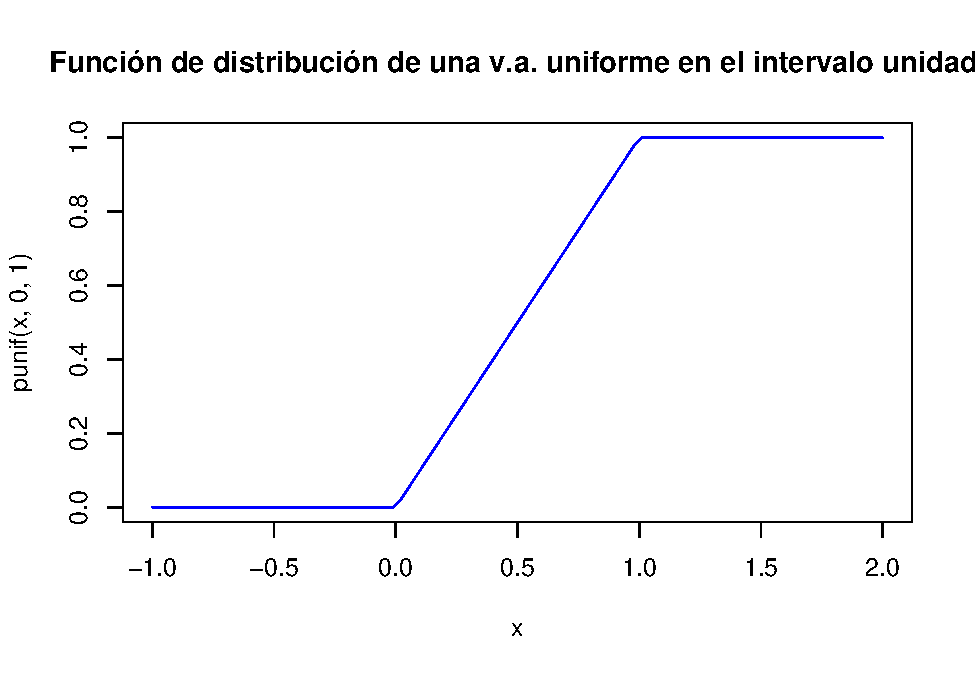
\includegraphics{curso-probabilidad-udemy_files/figure-latex/figUNIF-7} \end{center}

\hypertarget{propiedades-3}{%
\subsection{Propiedades}\label{propiedades-3}}

En las variables continuas los sucesos del tipo \(\{X\leq x \}\) y \(\{X< x \}\) tendrán la
misma probabilidad, y otros tipos de sucesos similares también, algunas de estas
propiedades se explicitan en la siguiente proposición.

\textbf{Propiedades}

Dada una v.a. continua \(X\) se tiene que:

\begin{itemize}
\tightlist
\item
  \(P(X\leq b)=P(X<b)\).
\item
  \(P(X<b)=P(X<a)+P(a<X<b)\).
\item
  \(P(a<X<b)=P(X<b)-P(X<a)\).
\end{itemize}

\textbf{Demostración:}

La primera es evidente \(P(X\leq b)=P(X<b)+P(X=b)=P(X<b)\).

Para demostrar la segunda, tenemos

\[\{X\leq a\}\cap \{a<X<b\}=\emptyset,\]
\[\{X\leq a\}\cup \{a<X<b\}=\{X<b\},\]
entonces
\begin{eqnarray*}
P(X< b) & = & P(\{X\leq a\}\cup \{a<X<b\})\\
& = & P(X\leq a)+P(a<X<b) \\
& = & P(X< a)+P(a<X<b).
\end{eqnarray*}

\textbf{Ejercicio}

La demostración de la tercera propiedad es similar a la segunda pero aplicando la primera. La dejamos como ejercicio.

\textbf{Propiedades de la función de distribución}

Las propiedades anteriores y combinaciones de ellas se pueden
escribir utilizando la función de distribución de \(X\):

 \textbf{Propiedades de la Función de Distribución}

Dada una variable aleatoria continua se tiene que:

\begin{itemize}
\tightlist
\item
  \(F_{X}(b)=F_{X}(a)+P(a<X<b)\).
\item
  \(P(a<X<b)=F_{X}(b)-F_{X}(a)\).
\item
  \(P(a\leq X\leq b)=F_{X}(b)-F_{X}(a)\).
\end{itemize}

\textbf{Ejercicio}
Se deja la demostración como ejercicio.

\textbf{Ejemplo: diana (continuación)}

En el ejemplo de la diana:

\[P(0.25<X<0.3)=F_{X}(0.3)-F_{X}(0.25)=0.3-0.25=0.05.\]

\hypertarget{funciuxf3n-de-densidad}{%
\subsection{Función de densidad}\label{funciuxf3n-de-densidad}}

 \textbf{Función de densidad}

Una función \(f:\mathbb{R}\to\mathbb{R}\) es una función de densidad sobre \(\mathbb{R}\) si cumple que

\begin{itemize}
\tightlist
\item
  \(f_{X}(x)\geq 0\) para todo \(x \in\mathbb{R}.\)
\item
  \(f\) es continua salvo a lo sumo en una cantidad finita de puntos sobre
  cada intervalo acotado de \(\mathbb{R}\).
\item
  \(\displaystyle\int\limits_{-\infty}^{+\infty} f_{X}(x) dx=1.\)
\end{itemize}

 \textbf{Función de distribución de una variable aleatoria}

Sea \(X\) una v.a. con función de distribución \(F_X\). Sea \(f:\mathbb{R}\to\mathbb{R}\) una función de densidad tal que

\[F_X(x)=\displaystyle\int_{-\infty}^{x} f_X(t)\,dt,\mbox{ para todo } x\in\mathbb{R}.\]

Entonces \(X\) es una variable aleatoria continua y \(f_X\) es la densidad de la v.a. \(X\).

El conjunto \(D_X=\{x\in\mathbb{R}| f_x(x)>0\}\) recibe el nombre de soporte o dominio de la
variable aleatoria continua y se interpreta como su conjunto de resultados posibles.

\textbf{Ejemplo: diana (continuación)}

En nuestro ejemplo, la función \(f\) es una densidad

\[
f_{X}(x)=\left\{
\begin{array}{ll}
0, & \mbox{si } x\leq 0,\\
1, & \mbox{si } 0 < x < 1,\\
0, & \mbox{si } 1\leq x,
\end{array}\right.
\]
que es la densidad de \(X\). En efecto:

\begin{itemize}
\item
  Si \(x \leq 0\), entonces \(\displaystyle\int_{-\infty}^x f_X(t) dt = 0.\)
\item
  Si \(0\leq x\leq 1\), entonces \(\displaystyle\int_{-\infty}^x f_X(t) dt = \int_0^x 1\, dt = x.\)
\item
  Si \(x\geq 1\), entonces \(\displaystyle\int_{-\infty}^x f_X(t) dt = \int_0^1 1\, dt = 1.\)
\end{itemize}

Por lo tanto, \(F_X(x)=\displaystyle\int_{-\infty}^x f_X(t) dt\) para todo \(x\in\mathbb{R}.\)

\begin{Shaded}
\begin{Highlighting}[]
\KeywordTok{curve}\NormalTok{(}\KeywordTok{dunif}\NormalTok{(x,}\DecValTok{0}\NormalTok{,}\DecValTok{1}\NormalTok{),}\DataTypeTok{xlim=}\KeywordTok{c}\NormalTok{(}\OperatorTok{-}\FloatTok{0.5}\NormalTok{,}\FloatTok{1.5}\NormalTok{),}\DataTypeTok{col=}\StringTok{"blue"}\NormalTok{,}
      \DataTypeTok{main=}\StringTok{"Densidad de la distribución uniforme en [0,1]"}\NormalTok{)}
\end{Highlighting}
\end{Shaded}

\begin{center}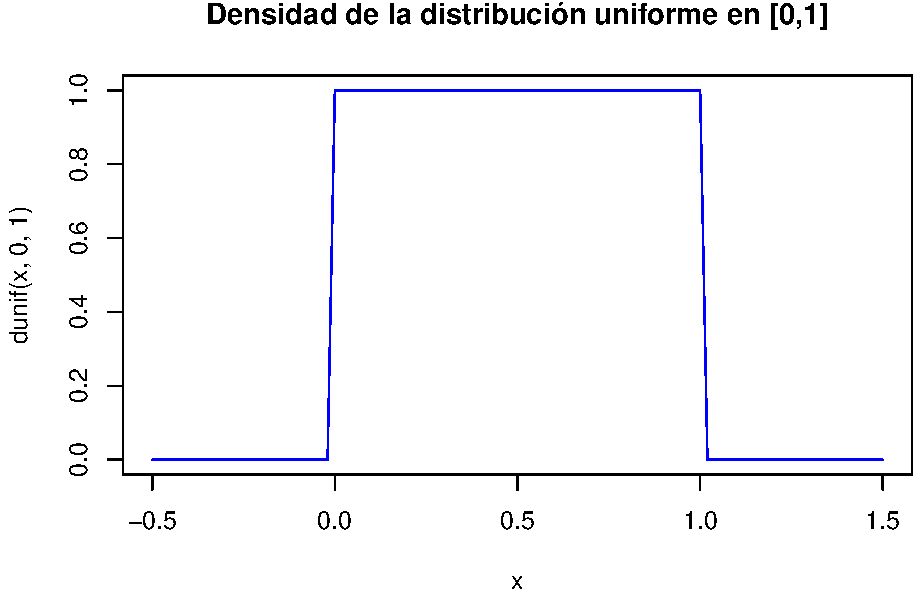
\includegraphics{curso-probabilidad-udemy_files/figure-latex/unnamed-chunk-10-1} \end{center}

\hypertarget{utilidad-de-la-funciuxf3n-de-densidad}{%
\subsection{Utilidad de la función de densidad}\label{utilidad-de-la-funciuxf3n-de-densidad}}

La función de densidad nos permite calcular diversas probabilidades.

\textbf{Propiedades de la función de densidad}

\begin{itemize}
\item
  Sea \(X\) una v.a. continua con función de distribución \(F_X\) y de
  densidad \(f_X\), entonces
  \begin{eqnarray*}
  P(a< X< b) &=&  P(a<X\leq b)= P(a\leq X< b)=\\
   & & P(a\leq X\leq b)= \displaystyle\int_{a}^b f_X(x) dx.
  \end{eqnarray*}
\item
  Si \(A\) es un subconjunto de \(\mathbb{R}\) entonces
\end{itemize}

\[
P(X\in A)=\displaystyle\int_{A} f(x) dx=\displaystyle\int_{A\cap D_X} f(x) dx.
\]

\textbf{Propiedades de la función de densidad}

Sea \(X\) una v.a. continua con función de distribución \(F_X\) y de densidad \(f_X\), entonces:

\begin{itemize}
\tightlist
\item
  Si \(f_x\) es continua en un punto \(x\), \(F_X\) es derivable en ese punto y
  \(F_X'(x)=f_X(x).\)
\item
  \(P(X=x)=0\) para todo \(x\in\mathbb{R}.\)
\end{itemize}

\textbf{Ejercicio}

Comprobar estas propiedades en el ejemplo de la diana.

\textbf{Ejemplo: tiempo ejecución de un proceso.}

Sea \(X=\) tiempo de ejecución de un proceso. Se supone que \(X\) sigue una distribución uniforme en dos unidades de tiempo, si tarda más el proceso se cancela.

Calculemos la función de densidad y de distribución de la v.a \(X\).

Entonces

\[
F_{X}(x)=P(X\leq x)=\frac{\mbox{Casos Favorables}}{\mbox{Casos Posibles}}=\frac{x}2.
\]

Luego su función de distribución es:

\[
F_{X}(x)=\left\{\begin{array}{ll}
0, & \mbox{si } x\leq 0,\\[1ex]
\frac{x}2, & \mbox{si } 0<x<2,\\[1ex]
1, & \mbox{si } 2\leq x.
\end{array}\right.
\]

Su función de densidad por su lado es:
\[
f_{X}(x)=F_{X}'(x)=\left\{\begin{array}{ll}
0, & \mbox{si } x\leq 0,\\[1ex]
\frac12, & \mbox{si } 0<x\leq 2,\\[1ex]
0, & \mbox{si } 2\leq x.
\end{array}\right.
\]

Efectivamente

\begin{itemize}
\item
  \(f_{X}(x)\geq 0,\) y tiene un conjunto finito de discontinuidades: \(\{0,2\}\).
\item
  \(F_X(x)=\int_{-\infty}^x f_X(t) dt,\) para todo \(x\in \mathbb{R}\). (Ejercicio: resolverlo gráficamente.)
\item
  \(\displaystyle\int\limits_{-\infty}^{+\infty}f_{X}(x)dx= \int\limits_0^2\frac12dx=\left[\frac{x}2\right]_0^2=\frac22-\frac02=1.\)
\end{itemize}

\textbf{Ejercicio: tiempo de un proceso}

Calcular la probabilidad de que uno de nuestros procesos tarde
más de una unidad de tiempo en ser procesado. Calcular también la probabilidad de
que dure entre \(0.5\) y \(1.5\) unidades de tiempo.

\hypertarget{esperanza-y-varianza-para-variables-aleatorias-continuas}{%
\subsection{Esperanza y varianza para variables aleatorias continuas}\label{esperanza-y-varianza-para-variables-aleatorias-continuas}}

Los mismos comentarios y definiciones que se dieron en la sección correspondiente del tema
de estadística descriptiva son aplicables aquí.

Así que sólo daremos las definiciones, la forma de cálculo y algunos ejemplos.

En lo que sigue, salvo que diagamos lo contrario, \(X\) es una v.a. continua con función de densidad \(f_{X}(x)\)

 \textbf{Esperanza v.a. continuas}

\begin{itemize}
\tightlist
\item
  Su esperanza es:
  \[E(X)=\displaystyle\int\limits_{-\infty}^{+\infty} x\cdot f_{X}(x)dx.\]
\item
  Si \(g(x)\) es una función de la variable \(X\) entonces:
  \[E(g(X))=\displaystyle\int\limits_{-\infty}^{+\infty} g(x)\cdot f_{X}(x)dx.\]
\end{itemize}

 \textbf{Varianza v.a. continuas}

\begin{itemize}
\tightlist
\item
  Su varianza es:
  \[
  Var(X)=\sigma_{X}^2=E((X-\mu_{X})^2)=
  \displaystyle\int\limits_{-\infty}^{+\infty} (x-\mu_{X})^2 f_{X}(x)dx.
  \]
\item
  Su desviación típica es: \[\sigma_{X}=+\sqrt{\sigma_{X}^2}.\]
\end{itemize}

 \textbf{Propiedades}

\begin{itemize}
\tightlist
\item
  \(\sigma_{X}^2\geq 0\).
\item
  \(Var(cte)=E(cte^2)-(E(cte))^2= cte^2 - cte^2=0\).
\item
  \(\displaystyle Var(x)=E(X^2)-\mu_{X}^2=\int\limits_{-\infty}^{+\infty}x^2 f_{X}(x)dx - \mu_{X}^2.\)
\item
  El mínimo de \(E((X-C)^2)\) se alcanza cuando \(C=E(X)\) y es \(Var(X)\).
\end{itemize}

\textbf{Ejemplo: diana (continuación)}

Calcular \(\mu_{X}\) y \(\sigma_{X}^2\) en el ejemplo de la diana.

Resultado
\[\mu_{X}=\frac12,\ E(X^2)=\frac13,\ Var(X)=\frac1{12}.\]

\textbf{Proposición}

Sea \(X\) una v.a. continua con \(E(X)=\mu_{X}\) y \(Var(X)=\sigma_{X}^2\) sea \(Y=a+b\cdot X\), donde
\(a,b\in\mathbb{R}\), es una nueva v.a. continua obtenida mediante una transformación lineal de \(X\).
Se verifican las mismas propiedades que en el caso discreto:

\begin{itemize}
\tightlist
\item
  \(E(Y)=E(a+b\cdot X)=a+b\cdot E(X)\).
\item
  \(Var(Y)=Var(a+b\cdot X)=b^2\cdot Var(X)\).
\item
  \(\sigma_{Y}=|b|\cdot \sigma_{X}\).
\item
  \(Z=\frac{X-\mu_{X}}{\sigma_{X}}\) es una transformación
  lineal de \(X\) de forma que
  \[E(Z)=0 \mbox{ y } Var(Z)=1.\]
\end{itemize}

\textbf{Ejemplo: venta de vinos}

En una empresa de venta de vinos por internet, sea
\(X\) el número de litros de vino del país vendidos en un año.
Supongamos que sabemos que \(E(X)=10000\) y que \(Var(X)=100\).
Supongamos que los gastos fijos de distribución son
50.000 € y el beneficio por litro es de 10 € por botella.
Definimos \(T=10 X-50000\) que será el beneficio después de gastos.

Entonces la esperanza del beneficio es
\[E(T)=10 E(X)-50000 = 50000,\]
y
\[Var(T)=10^2 Var(X)= 10000.\]

\hypertarget{transformaciones-de-variables-aleatorias}{%
\section{Transformaciones de variables aleatorias}\label{transformaciones-de-variables-aleatorias}}

Muchas variables aleatorias son funciones de otras v.a. En lo que sigue resumiremos diversas técnicas para dada una v.a. \(X\) y una
transformación \(Y=h(X)\) encontrar \(F_{Y}\) a
partir de \(F_{X}\).

\textbf{Tranformaciones de v.a. discretas}

Sea \(X\) una v.a. discreta con \(X(\Omega)=\{x_1,x_2,\ldots,x_{n},..\}\) y sea \(h:\mathbb{R}\to\mathbb{R}\) una aplicación.
Entonces \(Y=h(X)\) es también una v.a. discreta. Además si \(P_X\)
y \(F_{X}\) son las funciones de probabilidad y de distribución de
\(X\) entonces

\begin{itemize}
\tightlist
\item
  \(\displaystyle P_{Y}(y)=\sum_{x_{i}|h(x_{i})=y}P_X(x_{i}).\)
\item
  \(\displaystyle F_{Y}(y)=\sum_{x_{i}|h(x_{i})\leq y} P_X(x_{i}).\)
\end{itemize}

Desafortunadamente para variables no discretas, el resultado no es tan sencillo como la expresión anterior, pues la transformación de, por ejemplo, una v.a. continua puede ser continua, discreta, mixta, \(\ldots\)

\textbf{Transformación de v.a. continuas en continuas}

Sea \(X\) una v.a. continua cuya función de densidad es \(f_{X}\). Sea
\(h:\mathbb{R}\to\mathbb{R}\) una aplicación estrictamente monótona y derivable; por lo tanto, \(h'(x)\not=0\) para todo \(x\in\mathbb{R}\). Sea \(Y=h(X)\) la transformación de \(X\) por \(h\). Entonces \(Y\) es una v.a. continua con función de densidad

\[f_{Y}(y)=\left.\frac{f_{X}(x)}
{\left|h'(x)\right|}\right|_{x=h^{-1}(y)}.\]

\textbf{Densidad de una transformación de una v.a. continua}

Sea \(X\) una v.a. continua cuya función de densidad es \(f_{X}\). Sea
\[h:\mathbb{R}\to\mathbb{R},\]
una aplicación, no necesariamente monótona tal que :

\begin{itemize}
\tightlist
\item
  sea derivable con derivada no nula,
\item
  la ecuación \(h(x)=y\) tiene un número finito de soluciones
  \(x_1,x_2,..,x_{n}\),
\end{itemize}

entonces:

\[
\displaystyle f_{Y}(y)=\left.\sum_{k=1}^{n} \frac{f_{X}(x)}
{\left|h'(x)\right|}\right|_{x=x_{k}}.
\]

\textbf{Método general de transformación de v.a.}

Cuando no podamos aplicar las propiedades anteriores intentaremos
calcular primero la función de distribución de la transformación
y luego su densidad.

Notemos que en general si \(Y=g(X)\) es una v.a. transformación de la
v.a. \(X\) entonces

\[
F_{Y}(y)=P(Y\leq y)=P(g(X)\leq y).
\]

Por ejemplo, si \(g\) es estrictamente creciente y continua,

\[
F_{Y}(y)=P(g(X)\leq y)=P(X\leq g^{-1}(y))=F_{X}(g^{-1}(y)),
\]
y si \(g\) es estrictamente decreciente y continua,
\[
F_{Y}(y)=P(g(X)\leq y)=P(X\geq g^{-1}(y))=1-F_{X}(g^{-1}(y)).
\]

\hypertarget{desigualdades-de-markov-y-de-chebychev}{%
\section{Desigualdades de Markov y de Chebychev}\label{desigualdades-de-markov-y-de-chebychev}}

En esta sección distintas desigualdades que acotan determinadas probabilidades de
una variable aleatoria.

Estas desigualdades sirven en algunos casos para acotar probabilidades de determinados sucesos.

También son útiles desde el punto de vista teórico, por ejemplo para justificar que la varianza es una medida de la dispersión de
los datos.

\hypertarget{desigualdad-de-markov}{%
\subsection{Desigualdad de Markov}\label{desigualdad-de-markov}}

\textbf{Desigualdad de Markov}

Sea \(X\) una v.a. positiva con \(E(X)\) finita. Entonces

\[P(X\geq a)\leq \frac{E(X)}{a},\mbox{ para todo }a>0.\]

\textbf{Demostración}:

Si \(X\) es continua y solo toma valores positivos

\begin{eqnarray*}
E(X) &=& \int_{-\infty}^{+\infty} x\cdot  f_{X}(x) dx=  \int_0^{+\infty} x\cdot f_{X}(x) dx=  \int_0^{a} x\cdot  f_{X}(x) dx +\int_{a}^{+\infty} x\cdot f_{X}(x) dx \\
& &\geq   \int_{a}^{+\infty} x\cdot
f_{X}(x) dx \geq a \int_{a}^{+\infty}
f_{X}(x) dx = a \cdot  P(X\geq a),
\end{eqnarray*}
de donde se sigue que
\[P(X\geq a)\leq \frac{E(X)}{a}.\]

 \textbf{Corolario}

Sea \(X\) una v.a. con \(E(X)\) finita entonces para todo \(a>0\)

\[P(|X|\geq a )\leq \frac{E(|X|)}{a}.\]

\textbf{Ejercicio}

Demuestra el corolario anterior a partir de la desigualdad de Markov.

La desigualdad de Chebychev también se denomina de Chebyshov y en inglés Chebyshev.

\hypertarget{desigualdad-de-chebychev}{%
\subsection{Desigualdad de Chebychev}\label{desigualdad-de-chebychev}}

\textbf{Desigualdad de Chebychev}

La desigualdad de Chebychev también se denomina de Chebyshov y en inglés Chebyshev.

Sea \(X\) una v.a.con \(E(X)=\mu\) y \(Var(X)=\sigma^2\) entonces para todo \(a>0\),

\[P(|X-\mu|\geq a)\leq \frac{\sigma^2}{a^2}.\]

\textbf{Demostración}

Apliquemos la consecuencia de la desigualdad de Markov a la v.a.
no negativa \(Y^2=(X-\mu)^2\). Entonces

\[
P(Y^2\geq a^2) \leq 
\frac{E(Y^2)}{a^2}=\frac{E((X-\mu)^2)}{a^2}
= \frac{Var(X)}{a^2}=\frac{\sigma^2}{a^2}.
\]
Por otra parte

\[
P(Y^2\geq a^2)=P(|Y|\geq a)= P(|X-\mu|\geq a),
\]
hecho que, junto con la desigualdad anterior, demuestra el resultado.

 \textbf{Utilidad básica de la desigualdad de Chebychev}

Supongamos que \(X\) es una v.a. con \(Var(X)=0\). Entonces, aplicando la desigualdad anterior,
\[P(|X-E(X)|\geq a )=0,\mbox{ para todo }a>0,\]
lo que implica que
\[P(X=E(X))=1,\]
por lo que probabilidad de que \(X\) sea
constantemente \(E(X)\) es 1, hecho que nos confirma la utilidad de la varianza como una
medida de la dispersión de los datos.

\textbf{Ejemplo: tiempo de respuesta}

Se sabe que el tiempo de respuesta medio y la desviación típica de un sistema multiusuario son 15 y 3 unidades de tiempo, respectivamente. Entonces:
\[
P(|X-15|\geq 5)\leq \frac9{25}=0.36.
\]

Si substituimos \(a\) por \(a\cdot \sigma\) en la
desigualdad de Chebychev, nos queda:

\[
P(|X-\mu|\geq a \sigma)\leq
\frac{\sigma^2}{(a\sigma)^2}=\frac1{a^2},
\]
que es otra manera de expresar la desigualdad de Chebychev.

\textbf{Más formas de la desgualdad de Chebychev}

La desigualdad de Chebychev también se puede escribir de al menos dos maneras más:

\[
P(\mu-a\leq X\leq \mu+a)\geq 1-\frac{\sigma^2}{a^2},
\]
y tomado como \(a=k\cdot \sigma\),
\[
P(\mu-k\cdot \sigma\leq X\leq \mu+ k \cdot \sigma)\geq 1-\frac1{k^2}.
\]

Tomando la segunda expresión que hemos visto para la desigualdad de
Chebychev para distintos valores de \(k>0\), tenemos la siguiente tabla:

\begin{longtable}[]{@{}ll@{}}
\toprule
k & \(P(|X-E(X)|\geq k \cdot \sigma)\)\tabularnewline
\midrule
\endhead
1 & \(\leq 1\)\tabularnewline
2 & \(\leq 0.25\)\tabularnewline
3 & \(\leq 0.111\)\tabularnewline
4 & \(\leq 0.0025\)\tabularnewline
\bottomrule
\end{longtable}

Por ejemplo para \(k=2\), esta desigualdad se puede interpretar como que, dada una v.a. \(X\) con cualquier distribución que tenga \(E(X)\) y \(Var(X)\) finitos, \emph{la probabilidad de que un valor se aleje de la media \(\mu\) más de \(a=2\) desviaciones típicas es menor o igual que \(0.25\)}.

Es decir sólo el 25\% de los valores estarán alejados de la media
más de \(2\sigma\), ¡\emph{sea cual sea la distribución de la v.a.}!

\hypertarget{cuantiles-de-variables-aleatorias}{%
\section{Cuantiles de variables aleatorias}\label{cuantiles-de-variables-aleatorias}}

Si \(X\) es una v.a. con dominio \(D_X\) y \(0<q<1\), llamaremos cuantil de orden \(q\) al menor valor perteneciente al dominio \(x_q\in D_X\) tal que:
\[P(X\leq x_q)\geq q.\]

En \texttt{R}, cada distribución \(X\) tiene la función \texttt{qX(p,...)} que devuelve precisamente el cuantil \(x_p\) tal que \(P(X\leq x_p)\geq p.\)

Dada una variable aleatoria \(X\), si existe la inversa de la función de distribución de \(X\), \(F_X^{-1}\), el cuantil \(q\) sería el valor que tiene la función \(F_X^{-1}\) en \(q\): \(x_q=F^{-1}(q)\).

En caso de no existir la inversa, dado \(q\), definimos el conjunto \(F_X^{-1}(q)\) como:
\[
F_X^{-1}(q) =\{x\in\mathbb{R},\ |\ F_X(x)=q\}.
\]
Entonces el cuantil \(q\) sería el mínimo del conjunto anterior considerando sólo valores del dominio de la variable: \(x_q =\min_{x\in D_X}(F_X^{-1}(q))\).

\textbf{Ejemplo: variable aleatoria que nos da el resultado del lanzamiento de un dado}

Sea \(X\) la variable aleatoria uniforme discreta que nos da el número de puntos obtenidos en el lanzamiento de un dado (seis caras numeradas del 1 al 6).

Su dominio es \(D_X=\{1,2,3,4,5,6\}\) y su función de probabilidad es
\[
P_X(x)=P(X=x)=
\left\{
\begin{array}{ll}
 \frac{1}{6}, & \mbox{ si } x=1,2,3,4,5,6, \\
0, & \mbox{ en otro caso. }.
\end{array}
\right.
\]
Su función de distribución es:
\[
F_X(x)= P(X\leq x)=
\left\{
\begin{array}{ll}
0, & \mbox{ si } x<1, \\
\frac{k}{6} & \mbox{ si } k\leq x< k+1 \mbox{ para } x= 1,2,3,4,6, \\
 1, & \mbox{si  } x \geq 6.
\end{array}
\right.
\]

La función siguiente llamada \texttt{ddado} nos define la función de probabilidad de \(X\) para un dado de \(n\) caras:

\begin{Shaded}
\begin{Highlighting}[]
\NormalTok{ddado=}\ControlFlowTok{function}\NormalTok{(x,}\DataTypeTok{n=}\DecValTok{6}\NormalTok{) \{}
  \KeywordTok{sapply}\NormalTok{(x,}\DataTypeTok{FUN=}\ControlFlowTok{function}\NormalTok{(x) \{}
    \ControlFlowTok{if}\NormalTok{( x }\OperatorTok\StringTok{ }\KeywordTok{c}\NormalTok{(}\DecValTok{1}\OperatorTok{:}\NormalTok{n))\{}\KeywordTok{return}\NormalTok{(}\DecValTok{1}\OperatorTok{/}\NormalTok{n)\} }\ControlFlowTok{else}\NormalTok{ \{}\KeywordTok{return}\NormalTok{(}\DecValTok{0}\NormalTok{)\}\})}
\NormalTok{  \}}
\end{Highlighting}
\end{Shaded}

Por ejemplo, el valor de \(P_X(0.5)\) sería:

\begin{Shaded}
\begin{Highlighting}[]
\KeywordTok{ddado}\NormalTok{(}\FloatTok{1.5}\NormalTok{,}\DataTypeTok{n=}\DecValTok{6}\NormalTok{)}
\end{Highlighting}
\end{Shaded}

\begin{verbatim}
## [1] 0
\end{verbatim}

y los valores de \(P_X(i)\) para \(i=1,\ldots 10\) sería:

\begin{Shaded}
\begin{Highlighting}[]
\KeywordTok{ddado}\NormalTok{(}\DecValTok{1}\OperatorTok{:}\DecValTok{10}\NormalTok{,}\DataTypeTok{n=}\DecValTok{6}\NormalTok{)}
\end{Highlighting}
\end{Shaded}

\begin{verbatim}
##  [1] 0.1666667 0.1666667 0.1666667 0.1666667 0.1666667 0.1666667 0.0000000
##  [8] 0.0000000 0.0000000 0.0000000
\end{verbatim}

La función \texttt{pdado} nos da la función de distribución de \(X\):

\begin{Shaded}
\begin{Highlighting}[]
\NormalTok{pdado=}\ControlFlowTok{function}\NormalTok{(x,}\DataTypeTok{n=}\DecValTok{6}\NormalTok{) }
\NormalTok{  \{}
  \KeywordTok{sapply}\NormalTok{(x,}\DataTypeTok{FUN=}\ControlFlowTok{function}\NormalTok{(y)\{ }\ControlFlowTok{if}\NormalTok{ (y}\OperatorTok{<}\DecValTok{1}\NormalTok{)\{ }\KeywordTok{return}\NormalTok{(}\DecValTok{0}\NormalTok{)\}}\ControlFlowTok{else}\NormalTok{\{}\ControlFlowTok{if}\NormalTok{(y}\OperatorTok{>=}\NormalTok{n)\{}\KeywordTok{return}\NormalTok{(}\DecValTok{1}\NormalTok{)\} }\ControlFlowTok{else}
\NormalTok{  \{}\KeywordTok{return}\NormalTok{(}\KeywordTok{sum}\NormalTok{(}\KeywordTok{ddado}\NormalTok{(}\KeywordTok{c}\NormalTok{(}\DecValTok{1}\OperatorTok{:}\NormalTok{(}\KeywordTok{floor}\NormalTok{(y))),}\DataTypeTok{n=}\NormalTok{n)))\}\}\})}
\NormalTok{  \}}
\end{Highlighting}
\end{Shaded}

Los valores de \(F_X(i)\) para \(i=0,\ldots, 11\) serían:

\begin{Shaded}
\begin{Highlighting}[]
\KeywordTok{pdado}\NormalTok{(}\DecValTok{0}\OperatorTok{:}\DecValTok{11}\NormalTok{,}\DecValTok{6}\NormalTok{)}
\end{Highlighting}
\end{Shaded}

\begin{verbatim}
##  [1] 0.0000000 0.1666667 0.3333333 0.5000000 0.6666667 0.8333333 1.0000000
##  [8] 1.0000000 1.0000000 1.0000000 1.0000000 1.0000000
\end{verbatim}

A continuación, construímos la función \texttt{qdado} que nos calcula el cuantil \(p\), para \(0\leq p\leq 1\), de la variable \(X\) como el mínimo de la antiimagen de \(p\) mediante la función de distribución \(F_X^{-1}(p)\)

\begin{Shaded}
\begin{Highlighting}[]
\NormalTok{qdado=}\ControlFlowTok{function}\NormalTok{(p,}\DataTypeTok{n=}\DecValTok{6}\NormalTok{)\{}
\KeywordTok{sapply}\NormalTok{(p,}\DataTypeTok{FUN=}\ControlFlowTok{function}\NormalTok{(}\DataTypeTok{pp=}\NormalTok{p,}\DataTypeTok{nn=}\NormalTok{n) }
\NormalTok{  \{}
  \ControlFlowTok{if}\NormalTok{(pp}\OperatorTok{<}\DecValTok{0} \OperatorTok{|}\StringTok{ }\NormalTok{pp}\OperatorTok{>}\DecValTok{1}\NormalTok{) \{}\KeywordTok{return}\NormalTok{(}\OtherTok{NA}\NormalTok{)\}}
  \ControlFlowTok{else}\NormalTok{ \{}
\NormalTok{  aux=pp}\OperatorTok{>=}\KeywordTok{pdado}\NormalTok{(}\DecValTok{1}\OperatorTok{:}\NormalTok{n,nn)}
\NormalTok{  aux}
  \KeywordTok{ifelse}\NormalTok{(}\KeywordTok{all}\NormalTok{(}\OperatorTok{!}\NormalTok{aux),}\KeywordTok{return}\NormalTok{(}\DecValTok{1}\NormalTok{),}\KeywordTok{return}\NormalTok{(}\KeywordTok{max}\NormalTok{(}\KeywordTok{which}\NormalTok{(pp}\OperatorTok{>=}\KeywordTok{pdado}\NormalTok{(}\DecValTok{1}\OperatorTok{:}\NormalTok{n,nn)))))\}\}}
\NormalTok{)}
\NormalTok{\}}
\end{Highlighting}
\end{Shaded}

Si \(p=1.5\) o \(p=-1\), la función anterior nos devuelve \texttt{NA} ya que ni 1.5 ni -1 están entre 0 y 1:

\begin{Shaded}
\begin{Highlighting}[]
\KeywordTok{qdado}\NormalTok{(}\FloatTok{1.5}\NormalTok{)}
\end{Highlighting}
\end{Shaded}

\begin{verbatim}
## [1] NA
\end{verbatim}

\begin{Shaded}
\begin{Highlighting}[]
\KeywordTok{qdado}\NormalTok{(}\OperatorTok{-}\DecValTok{1}\NormalTok{)}
\end{Highlighting}
\end{Shaded}

\begin{verbatim}
## [1] NA
\end{verbatim}

Los cuantiles \(x_{0.1}\), \(x_{0.5}\) \(x_{0.6}\) y \(x_1\) son:

\begin{Shaded}
\begin{Highlighting}[]
\KeywordTok{qdado}\NormalTok{(}\KeywordTok{c}\NormalTok{(}\FloatTok{0.1}\NormalTok{,}\FloatTok{0.5}\NormalTok{,}\FloatTok{0.6}\NormalTok{,}\DecValTok{1}\NormalTok{))}
\end{Highlighting}
\end{Shaded}

\begin{verbatim}
## [1] 1 3 3 6
\end{verbatim}

\hypertarget{distribuciones-notables}{%
\chapter{Distribuciones Notables}\label{distribuciones-notables}}

En este tema estudiaremos diversos tipos de experimentos que son muy frecuentes y algunas de las variables aleatorias asociadas a ellos.

Estas variables reciben distintos nombres que aplicaremos sin distinción al tipo de población del experimento a la variable o a su función de probabilidad, densidad o distribución.

Empezaremos con las variables aleatorias discretas que se presentan con frecuencia ya que están relacionadas con situaciones muy comunes como el número de caras en varios lanzamiento de una moneda, el número de veces que una maquina funciona hasta que se estropea, el numero de clientes en una cola,\ldots{}

\hypertarget{distribuciones-discretas}{%
\section{Distribuciones discretas}\label{distribuciones-discretas}}

\hypertarget{distribuciuxf3n-de-bernoulli}{%
\subsection{Distribución de Bernoulli}\label{distribuciuxf3n-de-bernoulli}}

Consideremos un experimento con dos resultados posibles éxito (E) y
fracaso (F). El espacio de sucesos será \(\Omega=\{E,F\}\).

Supongamos que la probabilidad de éxito es \(P(E)=p\), y naturalmente \(P(F)=1-p=q\) con \(0<p<1\).

Consideremos la aplicación

\[
X:\Omega=\{E,F\}\to \mathbb{R},
\]
definida por \(X(E)=1,\ X(F)=0.\)

Su función de probabilidad es:
\[
P_{X}(x)=
\left\{
\begin{array}{ll} 1-p=q, & \mbox{si } x=0,\\
p, & \mbox{si } x=1,\\
0, & \mbox{en cualquier otro caso.}
\end{array}
\right.
\]

Su función de distribución es:
\[
F_{X}(x)=P(X\leq x)=
\left\{
\begin{array}{ll} 
0, & \mbox{si } x<0,\\
1-p=q, & \mbox{si } 0\leq x <1,\\
1, & \mbox{si } 1\leq x. \\
\end{array}
\right.
\]
Bajo estas condiciones diremos que \(X\) \textbf{es una v.a. Bernoulli} o que sigue una ley de \textbf{distribución de probabilidad Bernoulli} de parámetro \(p\).

Lo denotaremos por \(X\equiv Ber(p)\) o también \(X\equiv B(1,p).\)

A este tipo de experimentos (éxito/fracaso) se les denomina experimentos Bernoulli.

Fue su descubridor un científico suizo \href{https://es.wikipedia.org/wiki/Jakob_Bernoulli}{Jacob Bernoulli}, uno más de la de la conocida \href{https://es.wikipedia.org/wiki/Familia_Bernoulli}{familia de científicos suizos Bernoulli}.

\textbf{Esperanza de una v.a. \(X\) \(Ber(p)\)}

Su \textbf{valor esperado} es:
\[E(X)=\displaystyle\sum_{x=0}^1 x\cdot P(X=x)= 0\cdot(1-p)+1\cdot p=p.\]
Calculemos también \(E(X^2)\):

\[E(X^2)=\displaystyle\sum_{x=0}^1 x^2\cdot P(X=x)= 0^2\cdot(1-p)+1^2\cdot p=p.\]
\textbf{Varianza de una v.a. \(X\) \(Ber(p)\)}

Su \textbf{varianza} es:

\[Var(X)=E(X^2)-\left(E(X)\right)^2=p-p^2=p\cdot (1-p)=p\cdot q.\]
Su desviación típica es:
\[
\sqrt{Var(X)}=\sqrt{p \cdot (1-p)}.
\]

\textbf{Resumen v.a con distribución Bernoulli}

\begin{longtable}[]{@{}rl@{}}
\toprule
\begin{minipage}[b]{0.52\columnwidth}\raggedleft
\(X\) Bernoulli\strut
\end{minipage} & \begin{minipage}[b]{0.42\columnwidth}\raggedright
\(Ber(p)\)\strut
\end{minipage}\tabularnewline
\midrule
\endhead
\begin{minipage}[t]{0.52\columnwidth}\raggedleft
\(D_X=\)\strut
\end{minipage} & \begin{minipage}[t]{0.42\columnwidth}\raggedright
\(\{0,1\}\)\strut
\end{minipage}\tabularnewline
\begin{minipage}[t]{0.52\columnwidth}\raggedleft
\(P_X(x)=P(X=x)=\)\strut
\end{minipage} & \begin{minipage}[t]{0.42\columnwidth}\raggedright
\(\left\{\begin{array}{ll} q & \mbox{si } x=0\\ p & \mbox{si } x=1\\0 & \mbox{en otro caso}\end{array}\right.\)\strut
\end{minipage}\tabularnewline
\begin{minipage}[t]{0.52\columnwidth}\raggedleft
\(F_X(x)=P(X\leq X)=\)\strut
\end{minipage} & \begin{minipage}[t]{0.42\columnwidth}\raggedright
\(\left\{\begin{array}{ll} 0 & \mbox{ si } x<0\\q & \mbox{ si } 0\leq x<1\\1 & \mbox{ si } 1\leq x \end{array}\right.\)\strut
\end{minipage}\tabularnewline
\begin{minipage}[t]{0.52\columnwidth}\raggedleft
\(E(X)=p\)\strut
\end{minipage} & \begin{minipage}[t]{0.42\columnwidth}\raggedright
\(Var(X)=p\cdot q\)\strut
\end{minipage}\tabularnewline
\bottomrule
\end{longtable}

\textbf{Ejemplo de Distribución Bernoulli}

Veamos los cálculos básicos usando la distribución \(Ber(p=0.25)\) en \texttt{R}.

\begin{Shaded}
\begin{Highlighting}[]
\KeywordTok{dbinom}\NormalTok{(}\DecValTok{0}\NormalTok{,}\DataTypeTok{size=}\DecValTok{1}\NormalTok{,}\DataTypeTok{prob=}\FloatTok{0.25}\NormalTok{)}
\end{Highlighting}
\end{Shaded}

\begin{verbatim}
## [1] 0.75
\end{verbatim}

\begin{Shaded}
\begin{Highlighting}[]
\KeywordTok{dbinom}\NormalTok{(}\DecValTok{1}\NormalTok{,}\DataTypeTok{size=}\DecValTok{1}\NormalTok{,}\DataTypeTok{prob=}\FloatTok{0.25}\NormalTok{)}
\end{Highlighting}
\end{Shaded}

\begin{verbatim}
## [1] 0.25
\end{verbatim}

\begin{Shaded}
\begin{Highlighting}[]
\KeywordTok{rbinom}\NormalTok{(}\DataTypeTok{n=}\DecValTok{20}\NormalTok{,}\DataTypeTok{size =} \DecValTok{1}\NormalTok{,}\DataTypeTok{prob=}\FloatTok{0.25}\NormalTok{)}
\end{Highlighting}
\end{Shaded}

\begin{verbatim}
##  [1] 0 0 1 1 0 1 1 0 0 0 0 0 0 0 0 0 0 1 0 0
\end{verbatim}

El siguiente código dibuja las función de probabilidad y la de distribución de una \(Ber(p=0.25)\)

\begin{Shaded}
\begin{Highlighting}[]
\KeywordTok{par}\NormalTok{(}\DataTypeTok{mfrow=}\KeywordTok{c}\NormalTok{(}\DecValTok{1}\NormalTok{,}\DecValTok{2}\NormalTok{))}
\KeywordTok{plot}\NormalTok{(}\DataTypeTok{x=}\KeywordTok{c}\NormalTok{(}\DecValTok{0}\NormalTok{,}\DecValTok{1}\NormalTok{),}\DataTypeTok{y=}\KeywordTok{dbinom}\NormalTok{(}\KeywordTok{c}\NormalTok{(}\DecValTok{0}\NormalTok{,}\DecValTok{1}\NormalTok{),}\DataTypeTok{size=}\DecValTok{1}\NormalTok{,}\DataTypeTok{prob=}\FloatTok{0.25}\NormalTok{),}
     \DataTypeTok{ylim=}\KeywordTok{c}\NormalTok{(}\DecValTok{0}\NormalTok{,}\DecValTok{1}\NormalTok{),}\DataTypeTok{xlim=}\KeywordTok{c}\NormalTok{(}\OperatorTok{-}\DecValTok{1}\NormalTok{,}\DecValTok{2}\NormalTok{),}\DataTypeTok{xlab=}\StringTok{"x"}\NormalTok{,}
     \DataTypeTok{main=}\StringTok{"Función de probabilidad}\CharTok{\textbackslash{}n}\StringTok{ Ber(p=0.25)"}\NormalTok{)}
\KeywordTok{lines}\NormalTok{(}\DataTypeTok{x=}\KeywordTok{c}\NormalTok{(}\DecValTok{0}\NormalTok{,}\DecValTok{0}\NormalTok{,}\DecValTok{1}\NormalTok{,}\DecValTok{1}\NormalTok{),}\DataTypeTok{y=}\KeywordTok{c}\NormalTok{(}\DecValTok{0}\NormalTok{,}\FloatTok{0.75}\NormalTok{,}\DecValTok{0}\NormalTok{,}\FloatTok{0.25}\NormalTok{), }\DataTypeTok{type =} \StringTok{"h"}\NormalTok{, }\DataTypeTok{lty =} \DecValTok{2}\NormalTok{,}\DataTypeTok{col=}\StringTok{"blue"}\NormalTok{)}
\KeywordTok{curve}\NormalTok{(}\KeywordTok{pbinom}\NormalTok{(x,}\DataTypeTok{size=}\DecValTok{1}\NormalTok{,}\DataTypeTok{prob=}\FloatTok{0.25}\NormalTok{),}
      \DataTypeTok{xlim=}\KeywordTok{c}\NormalTok{(}\OperatorTok{-}\DecValTok{1}\NormalTok{,}\DecValTok{2}\NormalTok{),}\DataTypeTok{col=}\StringTok{"blue"}\NormalTok{,}
      \DataTypeTok{main=}\StringTok{"Función de distribución\textbackslash{}n Ber(p=0.25)"}\NormalTok{)}
\KeywordTok{par}\NormalTok{(}\DataTypeTok{mfrow=}\KeywordTok{c}\NormalTok{(}\DecValTok{1}\NormalTok{,}\DecValTok{1}\NormalTok{))}
\end{Highlighting}
\end{Shaded}

\begin{center}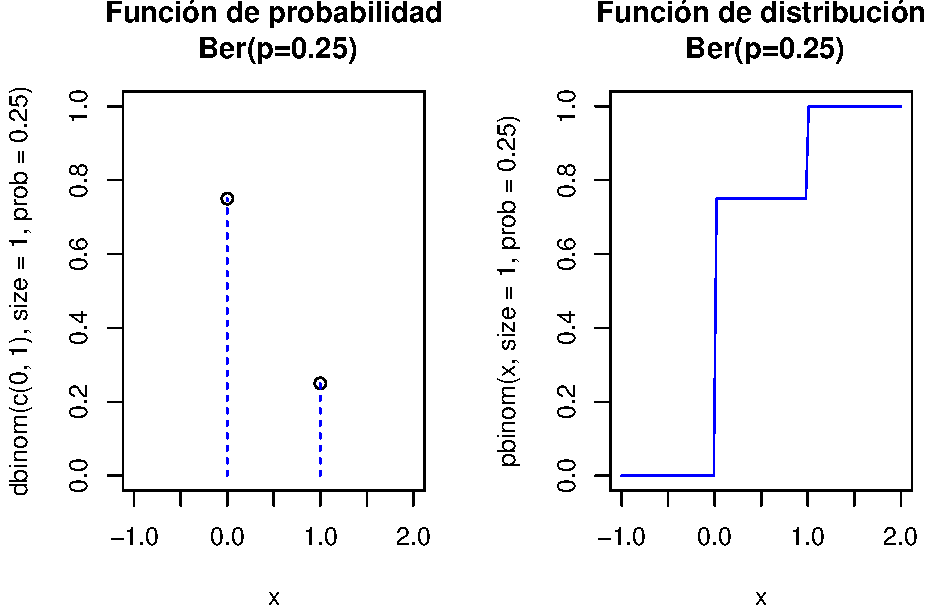
\includegraphics{curso-probabilidad-udemy_files/figure-latex/unnamed-chunk-20-1} \end{center}

\textbf{Gráficas interactivas \(Ber(p)\)}

Para ejecutar el siguiente gráfico interactivo, solamente tienes que cargar el paquete \texttt{shiny} en tu ordenador y luego copiar/pegar las siguientes instrucciones. De este modo podrás observar los cambios en las distribuciones variando los parámetros.

\begin{Shaded}
\begin{Highlighting}[]
\KeywordTok{sliderInput}\NormalTok{(}\StringTok{"p_ber"}\NormalTok{, }\DataTypeTok{label =} \StringTok{"Probabilidad éxito p:"}\NormalTok{,}
              \DataTypeTok{min =} \FloatTok{0.01}\NormalTok{, }\DataTypeTok{max =} \FloatTok{0.99}\NormalTok{, }\DataTypeTok{value =} \FloatTok{0.25}\NormalTok{, }\DataTypeTok{step =} \FloatTok{0.01}\NormalTok{)}

\KeywordTok{renderPlot}\NormalTok{(\{}
\KeywordTok{par}\NormalTok{(}\DataTypeTok{mfrow=}\KeywordTok{c}\NormalTok{(}\DecValTok{1}\NormalTok{,}\DecValTok{2}\NormalTok{))}
\NormalTok{  p=input}\OperatorTok{$}\NormalTok{p_ber}
\KeywordTok{plot}\NormalTok{(}\DataTypeTok{x=}\KeywordTok{c}\NormalTok{(}\DecValTok{0}\NormalTok{,}\DecValTok{1}\NormalTok{),}\DataTypeTok{y=}\KeywordTok{dbinom}\NormalTok{(}\KeywordTok{c}\NormalTok{(}\DecValTok{0}\NormalTok{,}\DecValTok{1}\NormalTok{),}\DataTypeTok{size=}\DecValTok{1}\NormalTok{,}\DataTypeTok{prob=}\NormalTok{p),}
     \DataTypeTok{ylim=}\KeywordTok{c}\NormalTok{(}\DecValTok{0}\NormalTok{,}\DecValTok{1}\NormalTok{),}\DataTypeTok{xlim=}\KeywordTok{c}\NormalTok{(}\OperatorTok{-}\FloatTok{0.5}\NormalTok{,}\DecValTok{2}\NormalTok{),}\DataTypeTok{xlab=}\StringTok{"x"}\NormalTok{,}\DataTypeTok{pch=}\DecValTok{21}\NormalTok{,}
     \DataTypeTok{main=}\KeywordTok{paste0}\NormalTok{(}\KeywordTok{c}\NormalTok{(}\StringTok{"Función de probabilidad}\CharTok{\textbackslash{}n}
\StringTok{                   Ber(p="}\NormalTok{,p,}\StringTok{")"}\NormalTok{),}\DataTypeTok{collapse=}\StringTok{""}\NormalTok{),}\DataTypeTok{bg=}\StringTok{"black"}\NormalTok{)}
\KeywordTok{segments}\NormalTok{(}\DataTypeTok{x0=}\DecValTok{0}\NormalTok{,}\DataTypeTok{y0=}\DecValTok{0}\NormalTok{,}\DataTypeTok{x1=}\DecValTok{0}\NormalTok{,}\DataTypeTok{y1=}\DecValTok{1}\OperatorTok{-}\NormalTok{p, }\DataTypeTok{col =} \StringTok{"blue"}\NormalTok{, }\DataTypeTok{lty =}\DecValTok{2}\NormalTok{)}
\KeywordTok{segments}\NormalTok{(}\DataTypeTok{x0=}\DecValTok{1}\NormalTok{,}\DataTypeTok{y0=}\DecValTok{0}\NormalTok{,}\DataTypeTok{x1=}\DecValTok{1}\NormalTok{,}\DataTypeTok{y1=}\NormalTok{p, }\DataTypeTok{col =} \StringTok{"blue"}\NormalTok{, }\DataTypeTok{lty =}\DecValTok{2}\NormalTok{)}
\KeywordTok{segments}\NormalTok{(}\DataTypeTok{x0=}\OperatorTok{-}\DecValTok{1}\NormalTok{,}\DataTypeTok{y0=}\DecValTok{1}\OperatorTok{-}\NormalTok{p,}\DataTypeTok{x1=}\DecValTok{0}\NormalTok{,}\DataTypeTok{y1=}\DecValTok{1}\OperatorTok{-}\NormalTok{p, }\DataTypeTok{col =} \StringTok{"blue"}\NormalTok{, }\DataTypeTok{lty =}\DecValTok{2}\NormalTok{)}
\KeywordTok{segments}\NormalTok{(}\DataTypeTok{x0=}\OperatorTok{-}\DecValTok{1}\NormalTok{,}\DataTypeTok{y0=}\NormalTok{p,}\DataTypeTok{x1=}\DecValTok{1}\NormalTok{,}\DataTypeTok{y1=}\NormalTok{p, }\DataTypeTok{col =} \StringTok{"blue"}\NormalTok{, }\DataTypeTok{lty =}\DecValTok{2}\NormalTok{)}
\NormalTok{x=}\DecValTok{0}\OperatorTok{:}\DecValTok{1}
\NormalTok{y=}\KeywordTok{pbinom}\NormalTok{(x,}\DataTypeTok{size=}\DecValTok{1}\NormalTok{,}\DataTypeTok{prob=}\NormalTok{p)}
\KeywordTok{curve}\NormalTok{(}\KeywordTok{pbinom}\NormalTok{(x,}\DataTypeTok{size=}\DecValTok{1}\NormalTok{,}\DataTypeTok{prob=}\NormalTok{p),}
      \DataTypeTok{xlim=}\KeywordTok{c}\NormalTok{(}\OperatorTok{-}\DecValTok{1}\NormalTok{,}\DecValTok{2}\NormalTok{),}\DataTypeTok{col=}\StringTok{"blue"}\NormalTok{,}
      \DataTypeTok{main=}\KeywordTok{paste0}\NormalTok{(}\KeywordTok{c}\NormalTok{(}\StringTok{"Función de distribución\textbackslash{}n Ber(p="}\NormalTok{,p,}\StringTok{")"}\NormalTok{),}\DataTypeTok{collapse=}\StringTok{""}\NormalTok{)}
\NormalTok{      )}

\KeywordTok{par}\NormalTok{(}\DataTypeTok{mfrow=}\KeywordTok{c}\NormalTok{(}\DecValTok{1}\NormalTok{,}\DecValTok{1}\NormalTok{))}
\NormalTok{\})}
\end{Highlighting}
\end{Shaded}

\hypertarget{distribuciuxf3n-binomial}{%
\subsection{Distribución binomial}\label{distribuciuxf3n-binomial}}

Si repetimos \(n\) veces de forma independiente un experimento Bernoulli de parámetro \(p\), el espacio muestral \(\Omega\) estará formado por cadenas de \(E\)'s y \(F\)'s de longitud \(n\).
Consideremos la v.a.:
\[X(\overbrace{EFFF\ldots EEF}^{n})=\mbox{número de éxitos en la cadena}.\]
A la variable aleatoria anterior se le conoce como distribución binomial de parámetros \(n\) y \(p\), y lo denotaremos por \(X\equiv B(n,p).\)

\textbf{Función de probabilidad de una binomial}

Su \textbf{función de probabilidad} es:
\[
P_{X}(x)=\left\{
\begin{array}{ll}
{n\choose x}\cdot  p^x \cdot(1-p)^{n-x}, &\mbox{ si } x=0,1,\ldots,n,\\
0,  & \mbox{ en otro caso.}
\end{array}\right.
\]
\textbf{Función de distribución de una binomial}

Su \textbf{función de distribución} no tiene una fórmula cerrada. Hay que acumular la función de probabilidad:
\[
\begin{array}{ll}
F_{X}(x)=P(X\leq x) & =  \sum_{i=0}^x P_X(i)\\
& = 
\left\{
\begin{array}{ll}
0, & \mbox{ si } x\leq 0,\\\displaystyle
\sum_{i=0}^k {n\choose i}\cdot  p^i \cdot (1-p)^{n-i} & \mbox{ si } 
\left\{
  \begin{array}{l} 
  k\leq x< k+1,\\
  k=0,1,\ldots,n,
  \end{array}
\right.\\
1, & \mbox{ si } n\leq x.
\end{array}
\right.
\end{array}
\]

\textbf{Números binomiales con R}

Los números binomiales calculan el número de equipos de baloncesto distintos que (\(k=5\) jugadores) se pueden hacer con 6 jugadores (\(n=6\)).

Es decir cuántas maneras distintas hay para elegir (\emph{choose}) 5 jugadores en un conjunto de 6 jugadores. Todo el mundo diría
¡¡¡6!!!. Efectivamente con \texttt{R} es

\begin{Shaded}
\begin{Highlighting}[]
\KeywordTok{choose}\NormalTok{(}\DecValTok{6}\NormalTok{,}\DecValTok{5}\NormalTok{)}
\end{Highlighting}
\end{Shaded}

\begin{verbatim}
## [1] 6
\end{verbatim}

Con 10 jugadores el número de equipos de 5 distintos es bastante más grande

\begin{Shaded}
\begin{Highlighting}[]
\KeywordTok{choose}\NormalTok{(}\DecValTok{10}\NormalTok{,}\DecValTok{5}\NormalTok{)}
\end{Highlighting}
\end{Shaded}

\begin{verbatim}
## [1] 252
\end{verbatim}

Y, por ejemplo, con un equipo de fútbol profesional que tiene en plantilla 22 jugadores (quitando los guardametas) se pueden formar ¡¡nada menos que!!

\begin{Shaded}
\begin{Highlighting}[]
\KeywordTok{choose}\NormalTok{(}\DecValTok{22}\NormalTok{,}\DecValTok{10}\NormalTok{)}
\end{Highlighting}
\end{Shaded}

\begin{verbatim}
## [1] 646646
\end{verbatim}

un bonito número capicúa que nos da el número de equipos distintos que se pueden formar.

Obviamente se tiene que una v.a. Bernoulli es una binomial con \(n=1\):
\(B(1,p)=Ber(p).\)

\textbf{Ejercicio}

Calculad las funciones de distribución de una binomial \(B(n=1,p=0.3)\) y comprobar que coinciden con las distribuciones de una \(Ber(p=0.3)\).

\textbf{Observaciones sobre la distribución binomial}

\begin{itemize}
\tightlist
\item
  La probabilidad de fracaso se suele denotar con \(q=1-p\), \textbf{sin ningún aviso adicional}, con el fin de acortar y agilizar la escritura de las fórmulas.
\item
  Su \textbf{función de distribución no tienen una formula general}, hay que calcularla con una función de R o python. En el siglo pasado se tabulaban en los libros de papel :-).
\item
  En el material adicional os pondremos unas tablas de esta distribución
  para distintos valores de \(n\) y \(p\) para que disfrutéis de tan ancestral método de cálculo.
\item
  Cualquier paquete estadístico u hoja de cálculo dispone de
  funciones para el cálculo de estas probabilidades, así que el \textbf{uso de las tablas} queda \textbf{totalmente anticuado}.
\end{itemize}

\textbf{Esperanza de una \(B(n,p)\)}

Su \textbf{esperanza} es:
\[E(X)=\displaystyle\sum_{k=0}^n k \cdot  {n \choose k }\cdot p^k\cdot q^{n-k} = n\cdot p.\]
La esperanza de \(X^2\) es:
\[
E(X^2)= \displaystyle\sum_{k=0}^n k^2 \cdot  {n \choose k }\cdot p^k\cdot q^{n-k}= n\cdot p\cdot q-(n\cdot p)^2.
\]

\textbf{Varianza de una \(B(n,p)\)}

Su \textbf{varianza} es:

\[Var(X)=E(X^2)-\left(E(X)\right)^2=n\cdot p \cdot q=n\cdot p\cdot (1-p).\]

Su desviación típica es:

\[\sqrt{n\cdot p\cdot q}=\sqrt{n\cdot p\cdot (1-p)}.\]

En temas posteriores veremos una forma sencilla del cálculo de la esperanza y varianza de una \(B(n,p)\) como las suma de \(n\) v.a. \(Ber(p)\) independientes.

\textbf{Ejercicio}

Justificar de forma intuitiva que si \(X_i\) con \(i=1,2,\ldots, n\) son v.a. \(Ber(p)\) independientes entonces \(X=\displaystyle\sum_{i=1}^n X_i\) sigue una distribución \(B(n,p).\)

\textbf{Resumen v.a con distribución binomial \(B(n,p)\)}

\begin{longtable}[]{@{}rll@{}}
\toprule
\begin{minipage}[b]{0.41\columnwidth}\raggedleft
\(X\) binomial\strut
\end{minipage} & \begin{minipage}[b]{0.26\columnwidth}\raggedright
\(B(n,p)\)\strut
\end{minipage} & \begin{minipage}[b]{0.24\columnwidth}\raggedright
\strut
\end{minipage}\tabularnewline
\midrule
\endhead
\begin{minipage}[t]{0.41\columnwidth}\raggedleft
\(D_X=\)\strut
\end{minipage} & \begin{minipage}[t]{0.26\columnwidth}\raggedright
\(\{0,1,\ldots n\}\)\strut
\end{minipage} & \begin{minipage}[t]{0.24\columnwidth}\raggedright
\strut
\end{minipage}\tabularnewline
\begin{minipage}[t]{0.41\columnwidth}\raggedleft
\(P_X(x)=P(X=x)=\)\strut
\end{minipage} & \begin{minipage}[t]{0.26\columnwidth}\raggedright
\(\left\{\begin{array}{ll}{n\choose x}\cdot p^x\cdot (1-p)^{n-x} & \mbox{ si } x=0,1,\ldots,n\\0 & \mbox{ en otro caso.}\end{array}\right.\)\strut
\end{minipage} & \begin{minipage}[t]{0.24\columnwidth}\raggedright
\strut
\end{minipage}\tabularnewline
\begin{minipage}[t]{0.41\columnwidth}\raggedleft
\(F_X(x)=P(X\leq X)=\)\strut
\end{minipage} & \begin{minipage}[t]{0.26\columnwidth}\raggedright
no tiene fórmula (utilizad funciones de \texttt{R} o python)\strut
\end{minipage} & \begin{minipage}[t]{0.24\columnwidth}\raggedright
\strut
\end{minipage}\tabularnewline
\begin{minipage}[t]{0.41\columnwidth}\raggedleft
\(E(X)=\)\strut
\end{minipage} & \begin{minipage}[t]{0.26\columnwidth}\raggedright
\(n\cdot p\)\strut
\end{minipage} & \begin{minipage}[t]{0.24\columnwidth}\raggedright
\strut
\end{minipage}\tabularnewline
\begin{minipage}[t]{0.41\columnwidth}\raggedleft
\(Var(X)=\)\strut
\end{minipage} & \begin{minipage}[t]{0.26\columnwidth}\raggedright
\(n\cdot p \cdot (1-p)\)\strut
\end{minipage} & \begin{minipage}[t]{0.24\columnwidth}\raggedright
\strut
\end{minipage}\tabularnewline
\bottomrule
\end{longtable}

\textbf{Cálculos binomial con R}

Veamos los cálculos básicos con funciones de R para una v.a \(X\) con distribución binomial \(B(n=10,p=0.25)\).

Si queremos calcular con \texttt{R} algún valor de la función de distribución como por ejemplo \(F_X(0)=P(X\leq 0)\), tenemos que hacer:

\begin{Shaded}
\begin{Highlighting}[]
\KeywordTok{pbinom}\NormalTok{(}\DecValTok{0}\NormalTok{,}\DataTypeTok{size=}\DecValTok{10}\NormalTok{,}\DataTypeTok{prob=}\FloatTok{0.25}\NormalTok{)}
\end{Highlighting}
\end{Shaded}

\begin{verbatim}
## [1] 0.05631351
\end{verbatim}

y si queremos por ejemplo \(F_X(4)=P(X\leq 4)\), tenemos que hacer:

\begin{Shaded}
\begin{Highlighting}[]
\KeywordTok{pbinom}\NormalTok{(}\DecValTok{4}\NormalTok{,}\DataTypeTok{size=}\DecValTok{10}\NormalTok{,}\DataTypeTok{prob=}\FloatTok{0.25}\NormalTok{)}
\end{Highlighting}
\end{Shaded}

\begin{verbatim}
## [1] 0.9218731
\end{verbatim}

Sin embargo, si queremos calcular algún valor de la función de probabilidad como por ejemplo \(P(X=0)\), tenemos que hacer:

\begin{Shaded}
\begin{Highlighting}[]
\KeywordTok{dbinom}\NormalTok{(}\DecValTok{0}\NormalTok{,}\DataTypeTok{size=}\DecValTok{10}\NormalTok{,}\DataTypeTok{prob=}\FloatTok{0.25}\NormalTok{)}
\end{Highlighting}
\end{Shaded}

\begin{verbatim}
## [1] 0.05631351
\end{verbatim}

o por ejemplo para \(P(X=4)\):

\begin{Shaded}
\begin{Highlighting}[]
\KeywordTok{dbinom}\NormalTok{(}\DecValTok{4}\NormalTok{,}\DataTypeTok{size=}\DecValTok{10}\NormalTok{,}\DataTypeTok{prob=}\FloatTok{0.25}\NormalTok{)}
\end{Highlighting}
\end{Shaded}

\begin{verbatim}
## [1] 0.145998
\end{verbatim}

\textbf{Generación de muestras aleatorias con R}

Generaremos una muestra aleatoria de 100 valores de una población con distribución \(B(20,0.5)\)

\begin{Shaded}
\begin{Highlighting}[]
\KeywordTok{set.seed}\NormalTok{(}\DecValTok{2019}\NormalTok{)}
\KeywordTok{rbinom}\NormalTok{(}\DecValTok{100}\NormalTok{,}\DataTypeTok{size =} \DecValTok{20}\NormalTok{,}\DataTypeTok{prob=}\FloatTok{0.5}\NormalTok{)}
\end{Highlighting}
\end{Shaded}

\begin{verbatim}
##   [1] 12 11  9 11  6  6 12  5  7 11 12 11  8  8 11 11  7 11  9 10  9 10 14  8  8
##  [26]  5 11 14 11 10 11  5 12  8  6  7  9 10  5 12 11  9 12 11 12 10 13 13  8  8
##  [51]  9  7  6  9 10  9 16 13  6  6  8  8 11  9 12 15  9  7 12 11  9  8  9  8 11
##  [76] 15  7 10  9 12  6 13 14  8 10  8 10 11 11  9 10 11 12  8 10 12  9 13  9 13
\end{verbatim}

\textbf{Ejemplo}

El ejemplo anterior correspondería a repetir 100 veces el experimento de lanzar una moneda 20 veces y contar el número de caras.

\textbf{Cálculos distribución binomial con python}

Veamos los cálculos básicos con funciones de python para una v.a \(X\) con distribución binomial \(B(n=10,p=0.25)\).

Primero importamos la función \texttt{binom} de la librería \texttt{scipy.stat}:

\begin{Shaded}
\begin{Highlighting}[]
\ImportTok{from}\NormalTok{ scipy.stats }\ImportTok{import}\NormalTok{ binom}
\end{Highlighting}
\end{Shaded}

En general en el paquete \texttt{scipy}, la función de probabilidad se invocará con el método \texttt{pmf}, la de distribución con el método \texttt{cdf} mientras que una muestra aleatoria que siga esta distribución con el método \texttt{rvs}. En todos ellos aparecerá siempre el parámetro \texttt{loc} que se utiliza para desplazar el dominio de la variable aleatoria. Por ejemplo, en este caso:

\begin{Shaded}
\begin{Highlighting}[]
\NormalTok{binom.pmf(k, n, p, loc) }\OperatorTok{=}\NormalTok{  binom.pmf(k }\OperatorTok{-}\NormalTok{ loc, n, p)}
\end{Highlighting}
\end{Shaded}

Para calcular los valores de la función de distribución como por ejemplo \(F_X(0)=P(X\leq 0)\) y \(F_X(4)=P(X\leq 4)\) utilizamos la función \texttt{cdf}:

\begin{Shaded}
\begin{Highlighting}[]
\NormalTok{binom.cdf(}\DecValTok{0}\NormalTok{,n}\OperatorTok{=}\DecValTok{10}\NormalTok{,p}\OperatorTok{=}\FloatTok{0.25}\NormalTok{)}
\end{Highlighting}
\end{Shaded}

\begin{verbatim}
## 0.056313514709472656
\end{verbatim}

\begin{Shaded}
\begin{Highlighting}[]
\NormalTok{binom.cdf(}\DecValTok{4}\NormalTok{,n}\OperatorTok{=}\DecValTok{10}\NormalTok{,p}\OperatorTok{=}\FloatTok{0.25}\NormalTok{)}
\end{Highlighting}
\end{Shaded}

\begin{verbatim}
## 0.92187309265136719
\end{verbatim}

Notemos que al no indicar el valor de \texttt{loc}, se le asume que toma el valor 0.

Para calcular los valores de la función de probabilidad \(P(X=0)\) y \(P(X=4)\) utilizamos la función \texttt{pmf}:

\begin{Shaded}
\begin{Highlighting}[]
\NormalTok{binom.pmf(}\DecValTok{0}\NormalTok{,n}\OperatorTok{=}\DecValTok{10}\NormalTok{,p}\OperatorTok{=}\FloatTok{0.25}\NormalTok{)}
\end{Highlighting}
\end{Shaded}

\begin{verbatim}
## 0.056313514709472684
\end{verbatim}

\begin{Shaded}
\begin{Highlighting}[]
\NormalTok{binom.pmf(}\DecValTok{4}\NormalTok{,n}\OperatorTok{=}\DecValTok{10}\NormalTok{,p}\OperatorTok{=}\FloatTok{0.25}\NormalTok{)}
\end{Highlighting}
\end{Shaded}

\begin{verbatim}
## 0.14599800109863295
\end{verbatim}

Notemos que al no indicar el valor de \texttt{loc}, se le asume que toma el valor 0.

Si queremos generar una muestras aleatorias que siga una distribución binomial, podemos usar la función \texttt{rvs}. En este caso, generaremos una muestra aleatoria de 100 valores de una población \(B(20,0.5)\)

\begin{Shaded}
\begin{Highlighting}[]
\NormalTok{binom.rvs(n}\OperatorTok{=}\DecValTok{20}\NormalTok{,p}\OperatorTok{=}\FloatTok{0.25}\NormalTok{,size }\OperatorTok{=} \DecValTok{100}\NormalTok{)}
\end{Highlighting}
\end{Shaded}

\begin{verbatim}
## array([ 5,  4,  4,  4,  7, 11,  4,  4,  4,  5,  4,  6,  5,  0,  9,  5,  7,
##         4,  7,  1,  2,  7,  0,  6,  7,  8,  7,  5,  3,  2,  4,  1,  4,  2,
##         3,  5,  8,  7,  5,  6,  5,  5,  4,  5,  5,  5,  3,  3,  5,  4,  8,
##         5,  4,  5,  4,  1,  6,  5,  7,  4,  7,  5,  4,  9,  5,  3,  2,  5,
##         6,  2,  5,  6,  4,  4,  2,  5,  5,  4,  7,  5,  6,  8,  2,  5,  4,
##         9,  5,  5,  5,  6,  5,  5,  3,  4,  3,  5,  7,  9,  3,  6])
\end{verbatim}

 \textbf{Observación}

Notemos que la secuencia aleatoria generada no es la misma que con \texttt{R}. De hecho, si volvemos a ejecutar esta función obtendremos una muestra aleatoria distinta.

\begin{Shaded}
\begin{Highlighting}[]
\NormalTok{binom.rvs(n}\OperatorTok{=}\DecValTok{20}\NormalTok{,p}\OperatorTok{=}\FloatTok{0.25}\NormalTok{,size }\OperatorTok{=} \DecValTok{100}\NormalTok{)}
\end{Highlighting}
\end{Shaded}

\begin{verbatim}
## array([ 6, 10,  7,  3,  6,  4,  8,  6,  1,  5,  8,  4,  3,  3,  6,  5,  5,
##         6,  3,  4,  3,  4,  5,  3,  5,  4,  6,  4,  5,  4,  6,  4,  3,  7,
##         9,  7,  5,  6,  6,  3,  7,  4,  5,  2,  6,  4,  4,  5,  7,  4,  4,
##         3,  7,  1,  5,  6,  5,  3,  6,  7,  6,  2,  4,  4,  3,  3,  8,  6,
##         4,  7,  6,  2,  5,  7,  6,  7,  6,  5,  8,  3,  1, 10,  4,  4,  7,
##         8,  3,  8,  7,  3,  3,  5,  9,  6,  5,  5,  4,  5,  7,  3])
\end{verbatim}

Veamos algunos cálculos básicos con funciones de python para la binomial \(B(n=10,p=0.25)\).

\begin{Shaded}
\begin{Highlighting}[]
\NormalTok{binom.cdf(}\DecValTok{5}\NormalTok{,n}\OperatorTok{=}\DecValTok{10}\NormalTok{,p}\OperatorTok{=}\FloatTok{0.25}\NormalTok{)}
\end{Highlighting}
\end{Shaded}

\begin{verbatim}
## 0.98027229309082031
\end{verbatim}

\begin{Shaded}
\begin{Highlighting}[]
\NormalTok{binom.pmf(}\DecValTok{1}\NormalTok{,n}\OperatorTok{=}\DecValTok{10}\NormalTok{,p}\OperatorTok{=}\FloatTok{0.25}\NormalTok{)}
\end{Highlighting}
\end{Shaded}

\begin{verbatim}
## 0.18771171569824247
\end{verbatim}

\begin{Shaded}
\begin{Highlighting}[]
\NormalTok{binom.rvs(n}\OperatorTok{=}\DecValTok{20}\NormalTok{,p}\OperatorTok{=}\FloatTok{0.25}\NormalTok{,size}\OperatorTok{=}\DecValTok{10}\NormalTok{)}
\end{Highlighting}
\end{Shaded}

\begin{verbatim}
## array([ 8,  6, 10,  4,  3,  3,  4,  6,  9,  5])
\end{verbatim}

\textbf{Gráficas de la distribución binomial con \texttt{R}}

El siguiente código de \texttt{R} dibuja las función de probabilidad y la de distribución de una \(B(n=10,p=0.25)\):

\begin{Shaded}
\begin{Highlighting}[]
\KeywordTok{par}\NormalTok{(}\DataTypeTok{mfrow=}\KeywordTok{c}\NormalTok{(}\DecValTok{1}\NormalTok{,}\DecValTok{2}\NormalTok{))}
\NormalTok{aux=}\KeywordTok{rep}\NormalTok{(}\DecValTok{0}\NormalTok{,}\DecValTok{22}\NormalTok{)}
\NormalTok{aux[}\KeywordTok{seq}\NormalTok{(}\DecValTok{2}\NormalTok{,}\DecValTok{22}\NormalTok{,}\DecValTok{2}\NormalTok{)]=}\KeywordTok{dbinom}\NormalTok{(}\KeywordTok{c}\NormalTok{(}\DecValTok{0}\OperatorTok{:}\DecValTok{10}\NormalTok{),}\DataTypeTok{size=}\DecValTok{10}\NormalTok{,}\DataTypeTok{prob=}\FloatTok{0.25}\NormalTok{)}
\KeywordTok{plot}\NormalTok{(}\DataTypeTok{x=}\KeywordTok{c}\NormalTok{(}\DecValTok{0}\OperatorTok{:}\DecValTok{10}\NormalTok{),}\DataTypeTok{y=}\KeywordTok{dbinom}\NormalTok{(}\KeywordTok{c}\NormalTok{(}\DecValTok{0}\OperatorTok{:}\DecValTok{10}\NormalTok{),}\DataTypeTok{size=}\DecValTok{10}\NormalTok{,}\DataTypeTok{prob=}\FloatTok{0.25}\NormalTok{),}
  \DataTypeTok{ylim=}\KeywordTok{c}\NormalTok{(}\DecValTok{0}\NormalTok{,}\DecValTok{1}\NormalTok{),}\DataTypeTok{xlim=}\KeywordTok{c}\NormalTok{(}\OperatorTok{-}\DecValTok{1}\NormalTok{,}\DecValTok{11}\NormalTok{),}\DataTypeTok{xlab=}\StringTok{"x"}\NormalTok{,}
  \DataTypeTok{main=}\StringTok{"Función de probabilidad}\CharTok{\textbackslash{}n}\StringTok{ B(n=10,p=0.25)"}\NormalTok{)}
\KeywordTok{lines}\NormalTok{(}\DataTypeTok{x=}\KeywordTok{rep}\NormalTok{(}\DecValTok{0}\OperatorTok{:}\DecValTok{10}\NormalTok{,}\DataTypeTok{each=}\DecValTok{2}\NormalTok{),}\DataTypeTok{y=}\NormalTok{aux, }\DataTypeTok{type =} \StringTok{"h"}\NormalTok{, }\DataTypeTok{lty =} \DecValTok{2}\NormalTok{,}\DataTypeTok{col=}\StringTok{"blue"}\NormalTok{)}
\KeywordTok{curve}\NormalTok{(}\KeywordTok{pbinom}\NormalTok{(x,}\DataTypeTok{size=}\DecValTok{10}\NormalTok{,}\DataTypeTok{prob=}\FloatTok{0.25}\NormalTok{),}
  \DataTypeTok{xlim=}\KeywordTok{c}\NormalTok{(}\OperatorTok{-}\DecValTok{1}\NormalTok{,}\DecValTok{11}\NormalTok{),}\DataTypeTok{col=}\StringTok{"blue"}\NormalTok{,}
  \DataTypeTok{main=}\StringTok{"Función de distribución\textbackslash{}n B(n=10,p=0.25)"}\NormalTok{)}
\KeywordTok{par}\NormalTok{(}\DataTypeTok{mfrow=}\KeywordTok{c}\NormalTok{(}\DecValTok{1}\NormalTok{,}\DecValTok{1}\NormalTok{))}
\end{Highlighting}
\end{Shaded}

\begin{center}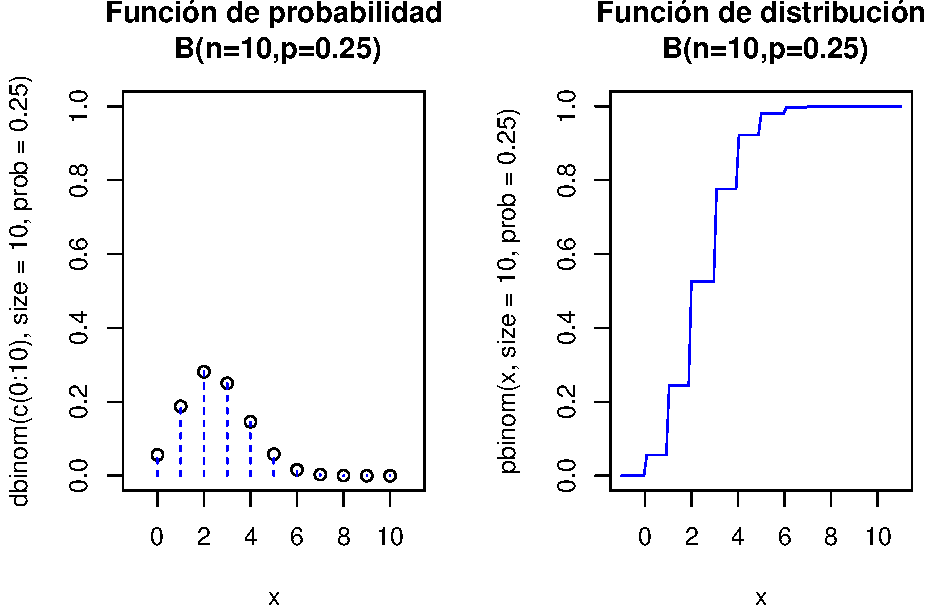
\includegraphics{curso-probabilidad-udemy_files/figure-latex/unnamed-chunk-29-1} \end{center}

\textbf{Gráficas interactivas de la distribución binomial}

Para ejecutar el siguiente gráfico interactivo, solamente tienes que cargar el paquete \texttt{shiny} en tu ordenador y luego copiar/pegar las siguientes instrucciones. De este modo podrás observar los cambios en las distribuciones variando los parámetros.

\begin{Shaded}
\begin{Highlighting}[]
\KeywordTok{fluidPage}\NormalTok{(}
\KeywordTok{fluidRow}\NormalTok{(}
  \KeywordTok{column}\NormalTok{(}\DecValTok{6}\NormalTok{,}
         \KeywordTok{sliderInput}\NormalTok{(}\StringTok{"n_binom"}\NormalTok{, }\DataTypeTok{label =} \StringTok{"Número de repeticiones n:"}\NormalTok{,}
              \DataTypeTok{min =} \DecValTok{1}\NormalTok{, }\DataTypeTok{max =} \DecValTok{50}\NormalTok{, }\DataTypeTok{value =}\DecValTok{10}\NormalTok{ , }\DataTypeTok{step =} \DecValTok{1}\NormalTok{)),}
  \KeywordTok{column}\NormalTok{(}\DecValTok{6}\NormalTok{,}
          \KeywordTok{sliderInput}\NormalTok{(}\StringTok{"p_binom"}\NormalTok{, }\DataTypeTok{label =} \StringTok{"Probabilidad éxito p:"}\NormalTok{,}
                     \DataTypeTok{min =} \FloatTok{0.01}\NormalTok{, }\DataTypeTok{max =} \FloatTok{0.99}\NormalTok{, }\DataTypeTok{value =} \FloatTok{0.25}\NormalTok{, }\DataTypeTok{step =} \FloatTok{0.01}\NormalTok{)}
\NormalTok{         )}
\NormalTok{  )}
\NormalTok{)}

\KeywordTok{renderPlot}\NormalTok{(\{}
\NormalTok{  n=input}\OperatorTok{$}\NormalTok{n_binom}
\NormalTok{  pr=input}\OperatorTok{$}\NormalTok{p_binom}
  
  \KeywordTok{par}\NormalTok{(}\DataTypeTok{mfrow=}\KeywordTok{c}\NormalTok{(}\DecValTok{1}\NormalTok{,}\DecValTok{2}\NormalTok{))}
\NormalTok{  aux=}\KeywordTok{rep}\NormalTok{(}\DecValTok{0}\NormalTok{,(n}\OperatorTok{+}\DecValTok{1}\NormalTok{)}\OperatorTok{*}\DecValTok{2}\NormalTok{)}
\NormalTok{  aux[}\KeywordTok{seq}\NormalTok{(}\DecValTok{2}\NormalTok{,(n}\OperatorTok{+}\DecValTok{1}\NormalTok{)}\OperatorTok{*}\DecValTok{2}\NormalTok{,}\DecValTok{2}\NormalTok{)]=}\KeywordTok{dbinom}\NormalTok{(}\KeywordTok{c}\NormalTok{(}\DecValTok{0}\OperatorTok{:}\NormalTok{n),}\DataTypeTok{size=}\NormalTok{n,}\DataTypeTok{prob=}\NormalTok{pr)}
  \KeywordTok{plot}\NormalTok{(}\DataTypeTok{x=}\KeywordTok{c}\NormalTok{(}\DecValTok{0}\OperatorTok{:}\NormalTok{n),}\DataTypeTok{y=}\KeywordTok{dbinom}\NormalTok{(}\KeywordTok{c}\NormalTok{(}\DecValTok{0}\OperatorTok{:}\NormalTok{n),}\DataTypeTok{size=}\NormalTok{n,}\DataTypeTok{prob=}\NormalTok{pr),}
       \DataTypeTok{ylim=}\KeywordTok{c}\NormalTok{(}\DecValTok{0}\NormalTok{,}\DecValTok{1}\NormalTok{),}\DataTypeTok{xlim=}\KeywordTok{c}\NormalTok{(}\OperatorTok{-}\DecValTok{1}\NormalTok{,n}\OperatorTok{+}\DecValTok{1}\NormalTok{),}\DataTypeTok{xlab=}\StringTok{"x"}\NormalTok{,}
       \DataTypeTok{main=}\KeywordTok{paste0}\NormalTok{(}\KeywordTok{c}\NormalTok{(}\StringTok{"Función de probabilidad}\CharTok{\textbackslash{}n}\StringTok{ B(n="}\NormalTok{,n,}\StringTok{",p="}\NormalTok{,pr,}\StringTok{")"}\NormalTok{),}\DataTypeTok{collapse =} \StringTok{""}\NormalTok{))}
  \KeywordTok{lines}\NormalTok{(}\DataTypeTok{x=}\KeywordTok{rep}\NormalTok{(}\DecValTok{0}\OperatorTok{:}\NormalTok{n,}\DataTypeTok{each=}\DecValTok{2}\NormalTok{),}\DataTypeTok{y=}\NormalTok{aux, }\DataTypeTok{type =} \StringTok{"h"}\NormalTok{, }\DataTypeTok{lty =} \DecValTok{2}\NormalTok{,}\DataTypeTok{col=}\StringTok{"blue"}\NormalTok{)}
  \KeywordTok{curve}\NormalTok{(}\KeywordTok{pbinom}\NormalTok{(x,}\DataTypeTok{size=}\NormalTok{n,}\DataTypeTok{p=}\NormalTok{pr),}
        \DataTypeTok{xlim=}\KeywordTok{c}\NormalTok{(}\OperatorTok{-}\DecValTok{1}\NormalTok{,n}\OperatorTok{+}\DecValTok{1}\NormalTok{),}\DataTypeTok{col=}\StringTok{"blue"}\NormalTok{,}
        \DataTypeTok{main=}\KeywordTok{paste0}\NormalTok{(}\KeywordTok{c}\NormalTok{(}\StringTok{"Función de distribución\textbackslash{}n B(n="}\NormalTok{,n,}\StringTok{",p="}\NormalTok{,pr,}\StringTok{")"}\NormalTok{),}
                    \DataTypeTok{collapse =} \StringTok{""}\NormalTok{))}
        \KeywordTok{par}\NormalTok{(}\DataTypeTok{mfrow=}\KeywordTok{c}\NormalTok{(}\DecValTok{1}\NormalTok{,}\DecValTok{1}\NormalTok{))}
\NormalTok{\})}
\end{Highlighting}
\end{Shaded}

\textbf{Gráficos de la distribución binomial con python}

\textbf{Ejercicio}

Buscad en la documentación de python cómo se dibuja la función de probabilidad y de distribución de una binomial y recread los gráficos anteriores.

Pista: Necesitaremos investigar más librerías:

\begin{Shaded}
\begin{Highlighting}[]
\ImportTok{import}\NormalTok{ numpy }\ImportTok{as}\NormalTok{ np}
\ImportTok{import}\NormalTok{ matplotlib.pyplot }\ImportTok{as}\NormalTok{ plt}
\end{Highlighting}
\end{Shaded}

\begin{Shaded}
\begin{Highlighting}[]
\NormalTok{n, p }\OperatorTok{=} \DecValTok{10}\NormalTok{, }\FloatTok{0.25}
\NormalTok{x }\OperatorTok{=}\NormalTok{ np.arange(binom.ppf(}\FloatTok{0.01}\NormalTok{, n, p),binom.ppf(}\FloatTok{0.99}\NormalTok{, n, p))}
\NormalTok{fig }\OperatorTok{=}\NormalTok{plt.figure(figsize}\OperatorTok{=}\NormalTok{(}\DecValTok{5}\NormalTok{, }\FloatTok{2.7}\NormalTok{))}
\NormalTok{ax }\OperatorTok{=}\NormalTok{ fig.add_subplot(}\DecValTok{1}\NormalTok{,}\DecValTok{2}\NormalTok{,}\DecValTok{1}\NormalTok{)}
\NormalTok{ax.plot(x, binom.pmf(x, n, p), }\StringTok{'bo'}\NormalTok{, ms}\OperatorTok{=}\DecValTok{8}\NormalTok{, label}\OperatorTok{=}\StringTok{'binom pmf'}\NormalTok{)}
\NormalTok{ax.vlines(x, }\DecValTok{0}\NormalTok{, binom.pmf(x, n, p), colors}\OperatorTok{=}\StringTok{'b'}\NormalTok{, lw}\OperatorTok{=}\DecValTok{5}\NormalTok{, alpha}\OperatorTok{=}\FloatTok{0.5}\NormalTok{)}
\ControlFlowTok{for}\NormalTok{ tick }\KeywordTok{in}\NormalTok{ ax.xaxis.get_major_ticks():}
\NormalTok{  tick.label.set_fontsize(}\DecValTok{5}\NormalTok{)}
\ControlFlowTok{for}\NormalTok{ tick }\KeywordTok{in}\NormalTok{ ax.yaxis.get_major_ticks():}
\NormalTok{  tick.label.set_fontsize(}\DecValTok{5}\NormalTok{) }
\NormalTok{ax }\OperatorTok{=}\NormalTok{ fig.add_subplot(}\DecValTok{1}\NormalTok{,}\DecValTok{2}\NormalTok{,}\DecValTok{2}\NormalTok{)}
\NormalTok{ax.plot(x, binom.cdf(x, n, p), }\StringTok{'bo'}\NormalTok{, ms}\OperatorTok{=}\DecValTok{8}\NormalTok{, label}\OperatorTok{=}\StringTok{'binom pmf'}\NormalTok{)}
\NormalTok{ax.vlines(x, }\DecValTok{0}\NormalTok{, binom.cdf(x, n, p), colors}\OperatorTok{=}\StringTok{'b'}\NormalTok{, lw}\OperatorTok{=}\DecValTok{5}\NormalTok{, alpha}\OperatorTok{=}\FloatTok{0.5}\NormalTok{)}
\ControlFlowTok{for}\NormalTok{ tick }\KeywordTok{in}\NormalTok{ ax.xaxis.get_major_ticks():}
\NormalTok{  tick.label.set_fontsize(}\DecValTok{5}\NormalTok{)}
\ControlFlowTok{for}\NormalTok{ tick }\KeywordTok{in}\NormalTok{ ax.yaxis.get_major_ticks():}
\NormalTok{  tick.label.set_fontsize(}\DecValTok{5}\NormalTok{)}
\NormalTok{fig.suptitle(}\StringTok{'Distribucion Binomial'}\NormalTok{)}
\NormalTok{plt.show()}
\end{Highlighting}
\end{Shaded}

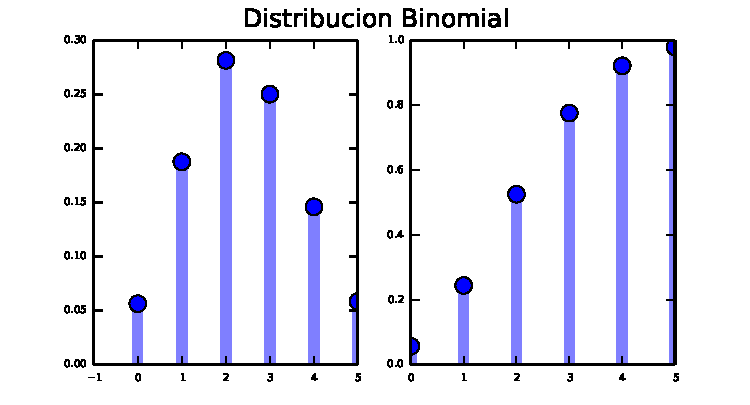
\includegraphics{curso-probabilidad-udemy_files/figure-latex/dibu_python2-1.pdf}

\textbf{Ejemplo: número de bolas rojas extraídas de una urna con reposición}

Tenemos una urna con \(100\) bolas de las cuales 40 son rojas y 60 son blancas. Extraemos al azar una bola, anotamos su color y la devolvemos a (reponemos en) la urna.

Supongamos que repetimos este proceso \(n=10\) reponiendo en cada ocasión la bola extraída.

Consideremos la variable aleatoria \(X\) como el número de bolas rojas extraídas (con reposición) en \(n=10\) repeticiones del mismo experimento de Bernoulli.

Bajo estas condiciones repetimos \(n=10\) veces el mismo experimento de Bernoulli con probabilidad de éxito (sacar bola roja)
\[P(Roja)=P(Éxito)=p=\frac{40}{100}=0.4.\]

Así que la variable \(X\) que es el número de bolas rojas extraídas de la urna (con reposición) en \(n=10\) ocasiones sigue una ley binomial \(B(n=10,p=0.4).\)

Nos preguntamos:

\begin{enumerate}
\def\labelenumi{\arabic{enumi}.}
\tightlist
\item
  ¿Cuál es la probabilidad de que saquemos exactamente \(4\) bolas rojas?
\item
  ¿Cuál es la probabilidad de que saquemos al menos \(4\) bolas rojas?
\item
  ¿Cuál es la probabilidad de que saquemos menos de \(3\) bolas rojas?
\item
  ¿Cuál es el valor esperado del número de bolas rojas?
\item
  ¿Cuál es la desviación típica del número de bolas rojas?
\end{enumerate}

\textbf{Solución 1}. ¿Cuál es la probabilidad de que saquemos exactamente \(4\) rojas?

Utilizando la función de probabilidad, tenemos que:
\[
\begin{array}{ll}
P(X=4)&={10\choose 4}\cdot 0.4^4\cdot (1-0.4)^{10-4}
= \frac{10!}{(10-4)!\cdot 4!}\cdot 0.4^4\cdot 0.6^6\\
&= \frac{7\cdot 8\cdot 9\cdot 10}{1\cdot 2\cdot 3\cdot 4}\cdot 0.4^4\cdot 0.6^6=0.2508227.
\end{array}
\]

Con \texttt{R}:

\begin{Shaded}
\begin{Highlighting}[]
\KeywordTok{dbinom}\NormalTok{(}\DecValTok{4}\NormalTok{,}\DataTypeTok{size=}\DecValTok{10}\NormalTok{,}\DataTypeTok{prob =} \FloatTok{0.4}\NormalTok{)}
\end{Highlighting}
\end{Shaded}

\begin{verbatim}
## [1] 0.2508227
\end{verbatim}

\textbf{Solución 2}. ¿Cuál es la probabilidad de que saquemos al menos \(4\) bolas rojas?

La probabilidad de sacar al menos 4 rojas se expresa como \(P(X \geq 4)=1-P(X<4)=1-P(X\leq 3):\)
\[
\begin{array}{rl}
P(X\leq 3)& = P(X=0)+P(X=1)+P(X=2)+P(X=3)\\
&= 
 {10\choose 0}\cdot 0.4^0\cdot (1-0.4)^{10-0}+ {10\choose 1}\cdot 0.4^1\cdot (1-0.4)^{10-1}\\
&+{10\choose 2}\cdot 0.4^2\cdot (1-0.4)^{10-2}+ {10\choose 3}\cdot 0.4^3\cdot (1-0.4)^{10-3}\\
&=0.3822806.
\end{array}
\]

Con \texttt{R}:

\begin{Shaded}
\begin{Highlighting}[]
\KeywordTok{pbinom}\NormalTok{(}\DecValTok{3}\NormalTok{,}\DecValTok{10}\NormalTok{,}\FloatTok{0.4}\NormalTok{)}
\end{Highlighting}
\end{Shaded}

\begin{verbatim}
## [1] 0.3822806
\end{verbatim}

Así que

\[P(X \geq 4 )=1-P(X< 4)=P(X\leq 3)=1-0.3822806=0.6177194.\]

Otra manera usando \texttt{R} sería:

\begin{Shaded}
\begin{Highlighting}[]
\DecValTok{1}\OperatorTok{-}\KeywordTok{pbinom}\NormalTok{(}\DecValTok{3}\NormalTok{,}\DecValTok{10}\NormalTok{,}\FloatTok{0.4}\NormalTok{)}
\end{Highlighting}
\end{Shaded}

\begin{verbatim}
## [1] 0.6177194
\end{verbatim}

Aunque en estos casos el parámetro \texttt{lower.tail\ =\ FALSE} es sin duda nuestra mejor opción:

\begin{Shaded}
\begin{Highlighting}[]
\KeywordTok{pbinom}\NormalTok{(}\DecValTok{3}\NormalTok{,}\DecValTok{10}\NormalTok{,}\FloatTok{0.4}\NormalTok{,}\DataTypeTok{lower.tail =} \OtherTok{FALSE}\NormalTok{)}
\end{Highlighting}
\end{Shaded}

\begin{verbatim}
## [1] 0.6177194
\end{verbatim}

\textbf{Solución 3}. ¿Cuál es la probabilidad de que saquemos menos de \(3\) bolas rojas?

\[
\begin{array}{ll}
P(X< 3)&= P(X\leq 2)=  P(X=0)+P(X=1)+P(X=2)\\
&=
{10\choose 0}\cdot 0.4^0\cdot (1-0.4)^{10-0}+ {10\choose 1}\cdot 0.4^1\cdot (1-0.4)^{10-1}\\
&+
{10\choose 2}\cdot 0.4^2\cdot (1-0.4)^{10-2}\\
&=0.1672898.
\end{array}
\]

En \texttt{R}:

\begin{Shaded}
\begin{Highlighting}[]
\KeywordTok{dbinom}\NormalTok{(}\DecValTok{0}\NormalTok{,}\DecValTok{10}\NormalTok{,}\FloatTok{0.4}\NormalTok{)}\OperatorTok{+}\KeywordTok{dbinom}\NormalTok{(}\DecValTok{1}\NormalTok{,}\DecValTok{10}\NormalTok{,}\FloatTok{0.4}\NormalTok{)}\OperatorTok{+}\KeywordTok{dbinom}\NormalTok{(}\DecValTok{2}\NormalTok{,}\DecValTok{10}\NormalTok{,}\FloatTok{0.4}\NormalTok{)}
\end{Highlighting}
\end{Shaded}

\begin{verbatim}
## [1] 0.1672898
\end{verbatim}

\begin{Shaded}
\begin{Highlighting}[]
\KeywordTok{pbinom}\NormalTok{(}\DecValTok{2}\NormalTok{,}\DecValTok{10}\NormalTok{,}\FloatTok{0.4}\NormalTok{)}
\end{Highlighting}
\end{Shaded}

\begin{verbatim}
## [1] 0.1672898
\end{verbatim}

\textbf{Solución 4}. ¿Cuál es el valor esperado del número de bolas rojas?

Como \(X\) es una \(B(n=10,p=0.4)\) sabemos que

\[E(X)=n\cdot p = 10\cdot 0.4=4.\]

Aunque en python tenemos la función \texttt{stats} que nos lo calcula directamente:

\begin{Shaded}
\begin{Highlighting}[]
\BuiltInTok{print}\NormalTok{(}\StringTok{"E(X) = }\SpecialCharTok{\{m\}}\StringTok{"}\NormalTok{.}\BuiltInTok{format}\NormalTok{(m}\OperatorTok{=}\NormalTok{binom.stats(n }\OperatorTok{=} \DecValTok{10}\NormalTok{, p }\OperatorTok{=} \FloatTok{0.4}\NormalTok{, moments}\OperatorTok{=}\StringTok{'m'}\NormalTok{)))}
\end{Highlighting}
\end{Shaded}

\begin{verbatim}
## E(X) = 4.0
\end{verbatim}

\textbf{Solución 5}. ¿Cuál es la desviación típica del número de bolas rojas?

La varianza es:
\[
Var(X)=n\cdot p \cdot(1-p)=10\cdot 0.4\cdot 0.6=2.4.
\]
Por lo tanto, la desviación típica es:

\[\sqrt{Var(X)}=\sqrt{2.4}= 1.5491933.\]

Aunque en python tenemos la función \texttt{stats} que nos lo calcula directamente:

\begin{Shaded}
\begin{Highlighting}[]
\BuiltInTok{print}\NormalTok{(}\StringTok{"Var(X) = }\SpecialCharTok{\{v\}}\StringTok{"}\NormalTok{.}\BuiltInTok{format}\NormalTok{(v}\OperatorTok{=}\NormalTok{binom.stats(n }\OperatorTok{=} \DecValTok{10}\NormalTok{, p }\OperatorTok{=} \FloatTok{0.4}\NormalTok{, moments}\OperatorTok{=}\StringTok{'v'}\NormalTok{)))}
\end{Highlighting}
\end{Shaded}

\begin{verbatim}
## Var(X) = 2.4
\end{verbatim}

\hypertarget{distribuciuxf3n-geomuxe9trica}{%
\subsection{Distribución geométrica}\label{distribuciuxf3n-geomuxe9trica}}

Todos hemos jugado a, por ejemplo, tirar una moneda hasta que obtengamos la primera cara.

O también tirar una pelota a una canasta de baloncesto hasta obtener la primera canasta.

Desde otro punto de vista también podemos intentar modelar el número de veces que accionamos una interruptor y la bombilla se ilumina hasta que falla.

O también el número de veces que un cajero automático nos da dinero hasta que falla.

La \textbf{modelización de este tipo de problemas se consigue con la llamada distribución geométrica}.

 \textbf{Distribución geométrica}

Repitamos un experimento Bernoulli, de parámetro \(p\), de forma independiente hasta obtener el primer éxito.

Sea \(X\) la v.a. que cuenta el número de fracasos antes del primer éxito. Por ejemplo que hayamos tenido \(x\) fracasos será una cadena de \(x\) fracasos culminada con un éxito. Más concretamente

\[P(\overbrace{FFF\ldots F}^{x}E)=P(F)^{x}\cdot P(E)=(1-p)^{x}\cdot p=q^{x}\cdot p.\]
Su función de probabilidad es:
\[
P_X(x)=P(X=x)=\left\{\begin{array}{ll}
(1-p)^{x}\cdot p, & \mbox{ si } x=0,1,2,\ldots,\\
0, &\mbox{ en otro caso.}
\end{array}\right.
\]
La v.a. definida anteriormente diremos que sigue una distribución geométrica de parámetro \(p\). La denotaremos por \(Ge(p)\).
Su dominio será: \(D_X=\{0,1,2,\ldots\}\).

Calculemos como ejemplo P(\(X\leq 3\)).
Por la propiedad de la probabilidad del suceso complementario tenemos que

\[
P(X\leq 3 )=1-P(X> 3)=1-P(X\geq 4)
\]

Efectivamente, el complementario del evento \(X\leq 3\) nos dice que hemos fracasado más de tres veces hasta conseguir el primer éxito, es decir, \textbf{hemos fracasado 4 o más veces}. Podemos simbolizar dicho evento de la forma siguiente:
\[
\{X>3\}=\{X\geq 4\}= \{FFFF\}
\]

Ahora, al ser los intentos independientes, tenemos que:
\[
\begin{array}{ll}
P(X>3) & =  P(\{FFFF\})= P(F)\cdot P(F)\cdot P(F)\cdot P(F)\\
&= (1-p)\cdot (1-p)\cdot (1-p)\cdot (1-p)= (1-p)^{3+1}=(1-p)^{4}.
\end{array}
\]

El valor de la función de distribución de \(X\) en \(x=3\) será, pues:
\[F_X(3)=P(X\leq 3)=1-P(X>3)=1-(1-p)^{3+1}.\]
Generalizando el resultado anterior a cualquier entero positivo \(k=0,1,2,\ldots\), tenemos:
\[F_X(k)=P(X\leq k)=1-(1-p)^{k+1},\mbox{ si } k=0,1,2,\ldots\]

En general, tendremos que:
\[
F_X(x)=P(X\leq x)=
\left\{\begin{array}{ll} 
0, & \mbox{ si } x<0,\\
1- (1-p),  & \mbox{ si } k=0\leq x <1,\\
1- (1-p)^2, & \mbox{ si } k=1\leq x <2,\\
1- (1-p)^3, & \mbox{ si } k=2\leq x <3,\\
1- (1-p)^{k+1}, & \mbox{ si } \left\{ \begin{array}{l}k\leq x< k+1,\\\mbox{para } k=0,1,2,\ldots\end{array}
    \right.\end{array}\right.
\]
De forma más compacta, tendremos que
\[
F_X(x)=P(X\leq x)=
\left\{\begin{array}{ll} 
0, & \mbox{ si } x<0,\\
1- (1-p)^{k+1}, & \mbox{ si } \left\{ \begin{array}{l}k\leq x< k+1,\\\mbox{para } k=0,1,2,\ldots\end{array}
    \right.\end{array}
    \right.
\]

Notemos que el límite de la función de distribución es:
\[
\displaystyle\lim_{k\to +\infty } F_X(k)=\lim_{k\to +\infty } 1-(1-p)^{k+1}=
1,
\]
ya que \(0<1-p<1\).

\textbf{Sumas derivadas series geométricas}

Recordemos las propiedades siguientes del tema de variables aleatorias:

\begin{itemize}
\tightlist
\item
  Si \(|r|<1\) también son convergentes las derivadas, respecto de \(r\), de la serie geométrica y convergen a la derivada correspondiente. Así, tenemos que:
  \[
  \begin{array}{ll}
  \left(\sum_{k=0}^{+\infty} r^k\right)' &= \sum_{k=1}^{+\infty}k\cdot
  r^{k-1}\\
  &= \left(\frac{1}{1-r}\right)'=\frac{1}{(1-r)^2}.\\
  \left(\sum_{k=0}^{+\infty} r^k\right)^{''} &= \sum_{k=2}^{+\infty}k \cdot(k-1)\cdot r^{k-2} \\
  &= \left(\frac{1}{1-r}\right)^{''}=\frac{2}{(1-r)^3}.
  \end{array}
  \]
\end{itemize}

\textbf{Esperanza de una v.a. \(Ge(p)\)}

Recordemos que \(P(X=x)=(1-p)^x\cdot p\) si \(x=0,1,2,\ldots\) y aplicado la fórmula anterior con \(r=1-p\), tenemos:
\[
\begin{array}{rll}
E(X)&=&\sum_{x=0}^{+\infty} x\cdot P_x(x)=\sum_{x=0}^{+\infty} x\cdot (1-p)^x\cdot p=
p\cdot (1-p) \cdot \sum_{x=1}^{+\infty} x\cdot (1-p)^{x-1}\\
&=& p\cdot (1-p)\cdot \frac{1}{(1-(1-p))^2}=p\cdot (1-p)\cdot \frac{1}{p^2}=\frac{1-p}{p}.
\end{array}
\]

\textbf{Valor \(E(X^2)\) de una v.a. \(Ge(p)\)}

\[
\begin{array}{rll}
E(X^2)&=&\sum_{x=0}^{+\infty} x^2\cdot P_X(x)=\sum_{x=1}^{+\infty} x^2\cdot (1-p)^x\cdot p\\
&=& 
\sum_{x=1}^{+\infty} (x\cdot (x-1)+x)\cdot (1-p)^{x}\cdot p\\
&=&
\sum_{x=1}^{+\infty} x\cdot (x-1)\cdot (1-p)^{x}\cdot p+\sum_{x=1}^{+\infty} x \cdot (1-p)^{x}\cdot p\\
&=&
(1-p)^{2}\cdot p\cdot \sum_{x=2}^{+\infty} x\cdot (x-1)\cdot (1-p)^{x-2}\\ 
& & +    (1-p)\cdot p\sum_{x=1}^{+\infty} x \cdot (1-p)^{x-1} 
\\  &=&
(1-p)^{2}\cdot p\cdot \sum_{x=2}^{+\infty} x\cdot (x-1)\cdot (1-p)^{x-2}\\ 
& &+   (1-p)\cdot p\sum_{x=1}^{+\infty} x \cdot (1-p)^{x-1}\\
&=&
p\cdot (1-p)^2 \frac{2}{(1-(1-p))^3}+  (1-p)\cdot p \frac{1}{(1-(1-p))^2}\\
&=&
p\cdot (1-p)^2 \frac{2}{p^3}+  (1-p)\cdot p \frac{1}{p^2}\\
&=&\frac{2\cdot (1-p)^2}{p^2}+\frac{1-p}{p}.
\end{array}
\]

\textbf{Varianza de una v.a. \(Ge(p)\)}

\[
\begin{array}{rll}
Var(X)&=&E(X^2)-E(X)^2=\frac{2\cdot (1-p)^2}{p^2}+\frac{1-p}{p}-\left(\frac{1-p}{p}\right)^2\\
&=&
\frac{2\cdot (1-p)^2+p\cdot(1-p)-(1-p)^2}{p^2}=\frac{(1-p)^2+p\cdot(1-p)}{p^2}\\
&=&
\frac{1-2\cdot p + p^2+p-p^2}{p^2}\\
&=& \frac{1-p}{p^2},
\end{array}
\]
y su desviación típica será
\[\sqrt{Var(X)}=\sqrt{\frac{1-p}{p^2}}.\]

\textbf{Resumen \(Ge(p)\) empezando en 0\$}

\begin{longtable}[]{@{}rl@{}}
\toprule
\begin{minipage}[b]{0.51\columnwidth}\raggedleft
\(X=\) Geométrica (empieza en \(0\))\strut
\end{minipage} & \begin{minipage}[b]{0.43\columnwidth}\raggedright
número de fracasos para conseguir el primer éxito\strut
\end{minipage}\tabularnewline
\midrule
\endhead
\begin{minipage}[t]{0.51\columnwidth}\raggedleft
\(D_X=\)\strut
\end{minipage} & \begin{minipage}[t]{0.43\columnwidth}\raggedright
\(\{0,1,\ldots n,\ldots\}\)\strut
\end{minipage}\tabularnewline
\begin{minipage}[t]{0.51\columnwidth}\raggedleft
\(P_X(x)=P(X=x)=\)\strut
\end{minipage} & \begin{minipage}[t]{0.43\columnwidth}\raggedright
\(\left\{\begin{array}{ll}(1-p)^{x}\cdot p, & \mbox{ si } x=0,1,2,\ldots \\0, & \mbox{ en otro caso.}\end{array}\right.\)\strut
\end{minipage}\tabularnewline
\begin{minipage}[t]{0.51\columnwidth}\raggedleft
\(F_X(x)=P(X\leq X)=\)\strut
\end{minipage} & \begin{minipage}[t]{0.43\columnwidth}\raggedright
\(\left\{\begin{array}{ll} 0 & \mbox{ si } x<0\\  1- (1-p)^{k+1}, & \mbox{ si } \left\{ \begin{array}{l}k\leq x< k+1,\\\mbox{para } k=0,1,2,\ldots\end{array}  \right.\end{array}\right.\)\strut
\end{minipage}\tabularnewline
\begin{minipage}[t]{0.51\columnwidth}\raggedleft
\(E(X)=\frac{1-p}{p}\)\strut
\end{minipage} & \begin{minipage}[t]{0.43\columnwidth}\raggedright
\(Var(X)=\frac{1-p}{p^2}\)\strut
\end{minipage}\tabularnewline
\bottomrule
\end{longtable}

\textbf{La variable geométrica que cuenta los intentos para obtener el primer éxito}

Supongamos que sólo estamos interesados en el \textbf{número de intentos} para obtener el primer éxito.

Si definimos \(Y\) como número de intentos para obtener el primer éxito, entonces \(Y=X+1\), donde \(X\equiv Ge(p)\).

Su dominio es \(D_Y=\{1,2,\ldots\}\)

La media se incrementa en un intento debido al éxito \(E(Y)=E(X+1)=E(X)+1=\frac{1-p}{p}+1=\frac1{p}\).

La varianza es la misma \(Var(Y)=Var(X+1)=Var(X)=\frac{1-p}{p^2}\).

\textbf{Resumen \(Ge(p)\) comenzando en \(1\)}

\begin{longtable}[]{@{}rl@{}}
\toprule
\begin{minipage}[b]{0.51\columnwidth}\raggedleft
\(Y\) geométrica (que cuenta el éxito empieza en 1)\strut
\end{minipage} & \begin{minipage}[b]{0.43\columnwidth}\raggedright
número de INTENTOS para OBTENER el primer éxito\strut
\end{minipage}\tabularnewline
\midrule
\endhead
\begin{minipage}[t]{0.51\columnwidth}\raggedleft
\(D_Y=\)\strut
\end{minipage} & \begin{minipage}[t]{0.43\columnwidth}\raggedright
\(\{1,2,\ldots n,\ldots\}\)\strut
\end{minipage}\tabularnewline
\begin{minipage}[t]{0.51\columnwidth}\raggedleft
\(P_Y(y)=P(Y=y)=\)\strut
\end{minipage} & \begin{minipage}[t]{0.43\columnwidth}\raggedright
\(\left\{\begin{array}{ll}(1-p)^{y-1}\cdot p, & \mbox{ si } y=1,2,3,\ldots\\ 0, & \mbox{ en otro caso.}\end{array}\right.\)\strut
\end{minipage}\tabularnewline
\begin{minipage}[t]{0.51\columnwidth}\raggedleft
\(F_Y(y)=P(Y\leq y)=\)\strut
\end{minipage} & \begin{minipage}[t]{0.43\columnwidth}\raggedright
\(\left\{\begin{array}{ll} 0, & \mbox{ si } y<1\\ 1- (1-p)^{k}, & \mbox{ si } \left\{ \begin{array}{l}k\leq y< k+1,\\\mbox{para } k=1,2,3,\dots \end{array} \right.\end{array}\right.\)\strut
\end{minipage}\tabularnewline
\begin{minipage}[t]{0.51\columnwidth}\raggedleft
\(E(X)=\frac1{p}\)\strut
\end{minipage} & \begin{minipage}[t]{0.43\columnwidth}\raggedright
\(Var(X)=\frac{1-p}{p^2}\)\strut
\end{minipage}\tabularnewline
\bottomrule
\end{longtable}

\textbf{Propiedad de la falta de memoria}

Sea \(X\) una v.a. discreta con dominio \(D_X=\{0,1,2,\ldots\}\), con \(P(X=0)=p\).

Entonces \(X\) sigue una ley \(Ge(p)\) si, y sólo si,
\[
P\left(X> k+j\big| X\geq j\right)=P(X> k)
\]
para todo \(k,j=0,1,2,3\ldots\).

\textbf{Demostración}

Si \(X\) es geométrica, entonces el lado derecho de la igualdad es

\[
P(X>k)=1-P(X\leq k)=1-\left(1-(1-p)^{k+1}\right)=(1-p)^{k+1},
\]
y el lado de izquierdo es:
\[
\begin{array}{rll} 
P\left(X> k+j\big| X\geq j\right)&=&\frac{P\left(\{X> k+j\}\cap \{X\geq j\} \right)}{P\left(X\geq j\right)}=
\frac{P\left(X>k+j \right)}{P\left(X\geq j \right)} = \frac{1-P(X\leq k+j)}{1-P(X\leq j-1)}\\
&=&  \frac{1-(1-(1-p)^{k+j+1})}{1-(1-(1-p)^{j-1+1})} =\frac{(1-p)^{k+j+1}}{(1-p)^{j}} = (1-p)^{k+1},
\end{array}
\]
lo que demuestra la igualdad.

Para demostrar el recíproco, tomemos \(j=1\) y \(k\geq 0\). Entonces, por la propiedad de la pérdida de memoria:
\[
P\left(X> k+1\big| X\geq 1\right)=P(X> k)
\]

Como \(P(X=0)=p\), tenemos que \(P(X \geq 1 )=1-P(X<1)=1-P(X=0)=1-p\).

Combinado las igualdades, tenemos que:
\[
P\left(X> k+1\big| X\geq 1\right)=\frac{P(X>k+1, X\geq 1)}{P(X\geq 1)}=\frac{P(X>k+1)}{P(X\geq 1)}=P(X>k).
\]
Así podemos poner que

\[
\begin{array}{rll}
P(X>k+1)&=&P(X\geq 1)\cdot P(X>k)=\left(1-P(X<1)\right)\cdot P(X>k)\\
&=&\left(1-P(X=0)\right)\cdot P(X>k)=(1-p)\cdot P(X>k).
\end{array}
\]

En general tenemos que:

\[
P(X>k+1)=(1-p)\cdot P(X>k).
\]
Del mismo modo para \(j=2\),
\[
P(X>k+2)=(1-p)\cdot P(X>k+1).
\]
Restando la primera igualdad de la última obtenemos:
\[
P(X>k+1)-P(X>k+2)=(1-p)\cdot P(X>k)-(1-p)\cdot P(X>k+1),
\]
de donde operando en cada lado de la igualdad obtenemos la recurrencia:
\[
[1-P(X\leq k+1)]-[1-P(X\leq k+2)]=(1-p)\cdot [P(X>k)-P(X>k+1)]
\]

Ahora operando,
\[
\begin{array}{rl}
P(X\leq k+2)-P(X\leq k+1) & =(1-p)\cdot[1-P(X\leq k)-\left(1-P(X\leq k+1)\right)],\\
P(X=k+2) & =(1-p)\cdot[P(X\leq k+1)-P(X\leq k)], \\
P(X=k+2) & =(1-p)\cdot P(X=k+1).
\end{array}
\]
De forma similar, obtenemos

\[
P(X=k+1)=(1-p)\cdot P(X=k).
\]
Utilizando la recurrencia anterior, podemos calcular todas las probabilidades \(P(X=k)\) a partir de la \(P(X=0)=p\):
\[
\begin{array}{rl}
P(X=0)&= p,\\
P(X=1)&=P(X=0+1)= (1-p)\cdot P(X=0) =(1-p)\cdot  p,\\
P(X=2)&=P(X=1+1)= (1-p)\cdot P(X=1)=(1-p)\cdot (1-p)\cdot p=(1-p)^2\cdot p,\\
 \vdots& \vdots \\
P(X=k)&=P(X=(k-1)+1)= (1-p)\cdot P(X=k-1)=(1-p)\cdot (1-p)^{k-1}\cdot p \\
& =(1-p)^{k}\cdot p,
\end{array}
\]
lo que demuestra el recíproco, es decir, que \(X\) es \(Geom(p)\).

 \textbf{Observación: Interpretación de la propiedad de la falta de memoria}

La propiedad de la falta de memoria
\[
P(X> k+j\big|X \geq j)=P(X > k),
\]\\
significa que, aunque \textbf{ya llevemos al menos \(j\) fracasos}, la probabilidad de \textbf{que fracasemos \(k\) veces más} no disminuye, es la misma que era cuando empezamos el experimento.

A este efecto se le suele etiquetar con la frase \textbf{el experimento carece de memoria} o es un \textbf{experimento sin memoria} (\emph{Memoryless Property}).

\textbf{Ejemplo falta de memoria}

Un ejemplo muy sencillo nos aclarará el alcance de esta propiedad es el ejercicio siguiente:

\textbf{Ejercicio: la llave que abre la puerta}

Tenemos un llavero con 10 llaves, sólo una de ellas abre una puerta. Cada vez que probamos una llave y falla olvidamos que llave hemos probado. ¿Cuál es la probabilidad de que si ya lo hemos intentado 5 veces necesitemos más de 4 intentos adicionales para abrir la puerta?

Tomemos \(k=4,j=5\), aplicando la propiedad de la falta de memoria

\[
P(X> 4+5/X \geq 5)=P(X > 4)
\]

Después de 5 fracasos no estamos ``más cerca'' de abrir la puerta.
La propiedad de la falta de memoria nos dice que en \textbf{después de cada intento es como si empezásemos de nuevo a abrir la puerta}. Tras 5 fracasos la probabilidad de que fallemos más de 4 veces más es la misma que cuando lo intentamos la primera vez.

¿Cuál es el número esperado de fracasos hasta abrir la puerta?

\[
E(X)=\frac{1-p}{p}=\frac{1-\frac{1}{10}}{\frac{1}{10}}=\frac{\frac{9}{10}}{\frac{1}{10}}=9.
\]

La varianza es
\[
Var(X)=\frac{1-p}{p^2}=\frac{1-\frac{1}{10}}{\left(\frac{1}{10}\right)^2}=\frac{\frac{9}{10}}{\frac{1}{100}}=
90.
\]

La desviación típica es \(\sqrt{90}=9.486833.\)

\textbf{Ejemplo: partidos hasta que el Barça gana al Madrid}

Los partidos Real Madrid vs FC Barcelona de \textbf{la liga} española se suelen denominar \textbf{El Clásico}, sean en el Bernabeu (estadio del Real Madrid) o en el Camp Nou (estadio del Barça)

Sea \(X\) la variable que cuenta el número de veces consecutivas que en un partido de fútbol de la liga el Barça no gana al Madrid sea en el Camp Nou o el Bernabeu.

Nuestra amiga Aina es muy culé (hincha del Barça) y quiere averiguar cuántos partidos consecutivos de \textbf{El Clásico} tiene que ver hasta ver ganar al Barça por primera vez.

Le interesa estimar cuánto le va a costar este capricho. Tendrá que comprar las entradas y pagar los viajes de Barcelona a Madrid.

En \href{https://es.wikipedia.org/wiki/El_Cl\%C3\%A1sico}{datos historicos de \textbf{El clásico} en la wikipedia} están los datos hasta el 3 de marzo de 2019: se han jugado en total 178 \textbf{Clásicos} donde el Real Madrid ganó en 72 ocasiones, el Barça, en 72 y empataron 34 veces.

La pregunta es: ¿Cuántos partidos se tienen que jugar de media para ver ganar al Barça por primera vez?

Con los datos anteriores, podemos estimar que la probabilidad de que el Barça gane un clásico cualquiera es:
\[P(\mbox{Barça})=\frac{72}{178}=0.4045.\]

Por tanto, podemos modelar la variable \(X\) con una ley geométrica con probabilidad de éxito \(p=P(\mbox{Barça})=\frac{72}{178}.\)

El número de partidos esperado para que el Barça gane por primera vez es:

\[E(X)=\frac{1-p}{p}=\frac{1-0.4045}{0.4045}=1.4722,\]
con una varianza de:
\[Var(X)=\frac{1-p}{p^2}=\frac{1-0.4045}{0.4045^2}=3.6397\]
y desviación típica:
\[\sqrt{3.6397}=1.9078.\]

\textbf{Cálculos con \texttt{R}}

Veamos los cálculos básicos con \texttt{R} para la distribución geométrica \(Ge(p=0.25)\). \texttt{R} implementa la geométrica que cuenta el número de fracasos, \(P(X=0)=(1-0.25)^0\cdot 0.25^1=0.25\):

\begin{Shaded}
\begin{Highlighting}[]
\KeywordTok{dgeom}\NormalTok{(}\DecValTok{0}\NormalTok{,}\DataTypeTok{prob=}\FloatTok{0.25}\NormalTok{)}
\end{Highlighting}
\end{Shaded}

\begin{verbatim}
## [1] 0.25
\end{verbatim}

\(P(X\leq 0)=1- (1-0.25)^{0+1}=1-0.75=0.25\):

\begin{Shaded}
\begin{Highlighting}[]
\KeywordTok{pgeom}\NormalTok{(}\DecValTok{0}\NormalTok{,}\DataTypeTok{prob=}\FloatTok{0.25}\NormalTok{)}
\end{Highlighting}
\end{Shaded}

\begin{verbatim}
## [1] 0.25
\end{verbatim}

\(P(X\leq 4)=1-(1-0.25)^{4+1}=1-0.75=1-0.75^5=0.7626953\):

\begin{Shaded}
\begin{Highlighting}[]
\KeywordTok{pgeom}\NormalTok{(}\DecValTok{4}\NormalTok{,}\DataTypeTok{prob=}\FloatTok{0.25}\NormalTok{)}
\end{Highlighting}
\end{Shaded}

\begin{verbatim}
## [1] 0.7626953
\end{verbatim}

Una muestra aleatoria de tamaño 25 de una \(Ge(0.25)\):

\begin{Shaded}
\begin{Highlighting}[]
\KeywordTok{rgeom}\NormalTok{(}\DataTypeTok{n=}\DecValTok{25}\NormalTok{,}\DataTypeTok{prob=}\FloatTok{0.25}\NormalTok{)}
\end{Highlighting}
\end{Shaded}

\begin{verbatim}
##  [1]  5  4  1  6 10  0  0 10  7  0  6  2  1  3  0  2  5  0  0  5  5  3  3  2  2
\end{verbatim}

\textbf{Gráficos con \texttt{R}}

\begin{Shaded}
\begin{Highlighting}[]
\KeywordTok{par}\NormalTok{(}\DataTypeTok{mfrow=}\KeywordTok{c}\NormalTok{(}\DecValTok{1}\NormalTok{,}\DecValTok{2}\NormalTok{))}
\NormalTok{x=}\KeywordTok{c}\NormalTok{(}\DecValTok{0}\OperatorTok{:}\DecValTok{10}\NormalTok{)}
\KeywordTok{plot}\NormalTok{(}\DataTypeTok{x=}\NormalTok{x,}\DataTypeTok{y=}\KeywordTok{dgeom}\NormalTok{(x,}\DataTypeTok{prob=}\FloatTok{0.25}\NormalTok{),}
  \DataTypeTok{ylim=}\KeywordTok{c}\NormalTok{(}\DecValTok{0}\NormalTok{,}\DecValTok{1}\NormalTok{),}\DataTypeTok{xlim=}\KeywordTok{c}\NormalTok{(}\OperatorTok{-}\DecValTok{1}\NormalTok{,}\DecValTok{11}\NormalTok{),}\DataTypeTok{xlab=}\StringTok{"x"}\NormalTok{,}
  \DataTypeTok{main=}\StringTok{"Función de probabilidad}\CharTok{\textbackslash{}n}\StringTok{ Ge(p=0.25)"}\NormalTok{)}
\KeywordTok{lines}\NormalTok{(}\DataTypeTok{x=}\KeywordTok{rep}\NormalTok{(}\DecValTok{0}\OperatorTok{:}\DecValTok{10}\NormalTok{,}\DataTypeTok{each=}\DecValTok{2}\NormalTok{),}\DataTypeTok{y=}\NormalTok{aux, }\DataTypeTok{type =} \StringTok{"h"}\NormalTok{, }\DataTypeTok{lty =} \DecValTok{2}\NormalTok{,}\DataTypeTok{col=}\StringTok{"blue"}\NormalTok{)}
\NormalTok{aux0=}\KeywordTok{dgeom}\NormalTok{(}\KeywordTok{c}\NormalTok{(}\DecValTok{0}\OperatorTok{:}\DecValTok{10}\NormalTok{),}\DataTypeTok{prob=}\FloatTok{0.25}\NormalTok{)}
\NormalTok{ceros=}\KeywordTok{rep}\NormalTok{(}\DecValTok{0}\NormalTok{,}\DecValTok{21}\NormalTok{)}
\NormalTok{ceros}
\NormalTok{aux=ceros}
\NormalTok{aux[}\DecValTok{2}\OperatorTok{*}\NormalTok{(}\KeywordTok{c}\NormalTok{(}\DecValTok{1}\OperatorTok{:}\DecValTok{11}\NormalTok{))]<-aux0}
\KeywordTok{curve}\NormalTok{(}\KeywordTok{pgeom}\NormalTok{(x,}\DataTypeTok{prob=}\FloatTok{0.25}\NormalTok{),}
  \DataTypeTok{xlim=}\KeywordTok{c}\NormalTok{(}\OperatorTok{-}\DecValTok{1}\NormalTok{,}\DecValTok{10}\NormalTok{),}\DataTypeTok{col=}\StringTok{"blue"}\NormalTok{,}
  \DataTypeTok{main=}\StringTok{"Función de distribución\textbackslash{}n Ge(p=0.25)"}\NormalTok{)}
\KeywordTok{par}\NormalTok{(}\DataTypeTok{mfrow=}\KeywordTok{c}\NormalTok{(}\DecValTok{1}\NormalTok{,}\DecValTok{1}\NormalTok{))}
\end{Highlighting}
\end{Shaded}

\begin{center}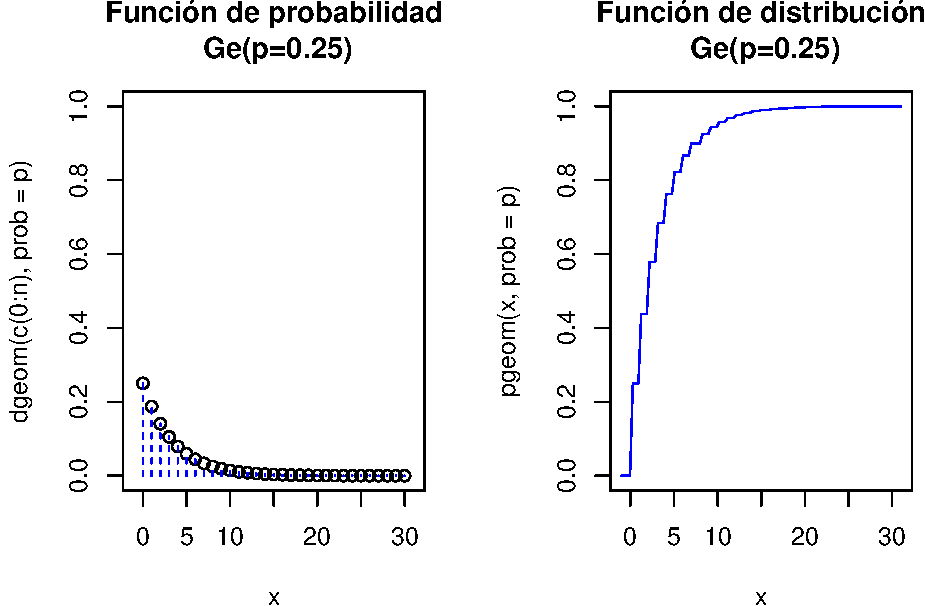
\includegraphics{curso-probabilidad-udemy_files/figure-latex/graficos22-1} \end{center}

\textbf{Gráficas interactivas geométrica}

Para ejecutar el siguiente gráfico interactivo, solamente tienes que cargar el paquete \texttt{shiny} en tu ordenador y luego copiar/pegar las siguientes instrucciones. De este modo podrás observar los cambios en las distribuciones variando los parámetros.

\begin{Shaded}
\begin{Highlighting}[]
\KeywordTok{sliderInput}\NormalTok{(}\StringTok{"p_geom"}\NormalTok{, }\DataTypeTok{label =} \StringTok{"Probabilidad de éxito:"}\NormalTok{,}
              \DataTypeTok{min =} \FloatTok{0.01}\NormalTok{, }\DataTypeTok{max =} \FloatTok{0.99}\NormalTok{, }\DataTypeTok{value =}\FloatTok{0.25}\NormalTok{ , }\DataTypeTok{step =} \FloatTok{0.01}\NormalTok{)}
\KeywordTok{renderPlot}\NormalTok{(\{}
  \KeywordTok{par}\NormalTok{(}\DataTypeTok{mfrow=}\KeywordTok{c}\NormalTok{(}\DecValTok{1}\NormalTok{,}\DecValTok{2}\NormalTok{))}
\NormalTok{  p=input}\OperatorTok{$}\NormalTok{p_geom}
\NormalTok{  n=}\DecValTok{30}
\NormalTok{  aux=}\KeywordTok{rep}\NormalTok{(}\DecValTok{0}\NormalTok{,(n}\OperatorTok{+}\DecValTok{1}\NormalTok{)}\OperatorTok{*}\DecValTok{2}\NormalTok{)}
\NormalTok{  aux[}\KeywordTok{seq}\NormalTok{(}\DecValTok{2}\NormalTok{,(n}\OperatorTok{+}\DecValTok{1}\NormalTok{)}\OperatorTok{*}\DecValTok{2}\NormalTok{,}\DecValTok{2}\NormalTok{)]=}\KeywordTok{dgeom}\NormalTok{(}\KeywordTok{c}\NormalTok{(}\DecValTok{0}\OperatorTok{:}\NormalTok{n),}\DataTypeTok{prob=}\NormalTok{p)}
  \KeywordTok{plot}\NormalTok{(}\DataTypeTok{x=}\KeywordTok{c}\NormalTok{(}\DecValTok{0}\OperatorTok{:}\NormalTok{n),}\DataTypeTok{y=}\KeywordTok{dgeom}\NormalTok{(}\KeywordTok{c}\NormalTok{(}\DecValTok{0}\OperatorTok{:}\NormalTok{n),}\DataTypeTok{prob=}\NormalTok{p),}
       \DataTypeTok{ylim=}\KeywordTok{c}\NormalTok{(}\DecValTok{0}\NormalTok{,}\DecValTok{1}\NormalTok{),}\DataTypeTok{xlim=}\KeywordTok{c}\NormalTok{(}\OperatorTok{-}\DecValTok{1}\NormalTok{,n}\OperatorTok{+}\DecValTok{1}\NormalTok{),}\DataTypeTok{xlab=}\StringTok{"x"}\NormalTok{,}
       \DataTypeTok{main=}\KeywordTok{paste0}\NormalTok{(}\KeywordTok{c}\NormalTok{(}\StringTok{"Función de probabilidad}\CharTok{\textbackslash{}n}\StringTok{ Ge(p="}\NormalTok{,p,}\StringTok{")"}\NormalTok{),}\DataTypeTok{collapse =} \StringTok{""}\NormalTok{))}
  \KeywordTok{lines}\NormalTok{(}\DataTypeTok{x=}\KeywordTok{rep}\NormalTok{(}\DecValTok{0}\OperatorTok{:}\NormalTok{n,}\DataTypeTok{each=}\DecValTok{2}\NormalTok{),}\DataTypeTok{y=}\NormalTok{aux, }\DataTypeTok{type =} \StringTok{"h"}\NormalTok{, }\DataTypeTok{lty =} \DecValTok{2}\NormalTok{,}\DataTypeTok{col=}\StringTok{"blue"}\NormalTok{)}
  \KeywordTok{curve}\NormalTok{(}\KeywordTok{pgeom}\NormalTok{(x,}\DataTypeTok{prob=}\NormalTok{p),}
        \DataTypeTok{xlim=}\KeywordTok{c}\NormalTok{(}\OperatorTok{-}\DecValTok{1}\NormalTok{,n}\OperatorTok{+}\DecValTok{1}\NormalTok{),}\DataTypeTok{col=}\StringTok{"blue"}\NormalTok{,}
        \DataTypeTok{main=}\KeywordTok{paste0}\NormalTok{(}\KeywordTok{c}\NormalTok{(}\StringTok{"Función de distribución\textbackslash{}n Ge(p="}\NormalTok{,p,}\StringTok{")"}\NormalTok{),}\DataTypeTok{collapse =} \StringTok{""}\NormalTok{))}
  \KeywordTok{par}\NormalTok{(}\DataTypeTok{mfrow=}\KeywordTok{c}\NormalTok{(}\DecValTok{1}\NormalTok{,}\DecValTok{1}\NormalTok{))}
\NormalTok{\})}
\end{Highlighting}
\end{Shaded}

\textbf{Cálculos con python}

Veamos los cálculos básicos con python para la distribución geométrica \(Ge(p=0.25)\). scipy.stats implementa la distribución geométrica que cuenta el número intentos así que empieza en 1.

Cargamos la función de la librería

\begin{Shaded}
\begin{Highlighting}[]
\ImportTok{from}\NormalTok{ scipy.stats }\ImportTok{import}\NormalTok{ geom}
\end{Highlighting}
\end{Shaded}

La función de probabilidad es \texttt{geom.pmf(x,p,loc=0)=geom.pmf(x,p)} es un geométrica que cuenta el número de intentos para obtener el primer éxito el valor por defecto del último parámetro es \texttt{loc=0}.

Si queremos la que cuenta el número de fracasos para obtener el primer éxito (la geométrica que empieza en 0) tenemos que usar \texttt{geom.pmf(x,p,loc=-1)}.

Es decir \texttt{geom.pmf(x,p,loc=-1)=geom.pmf(x-1,p,loc=0)}

Veamos pues los cálculos para la \(Ge(p)\) que empieza en \(0\).

\(P(X=0)=(1-0.25)^0\cdot 0.25^1=0.25\):

\begin{Shaded}
\begin{Highlighting}[]
\NormalTok{geom.pmf(}\DecValTok{0}\NormalTok{,p}\OperatorTok{=}\FloatTok{0.25}\NormalTok{,loc}\OperatorTok{=-}\DecValTok{1}\NormalTok{)}
\end{Highlighting}
\end{Shaded}

\begin{verbatim}
## 0.25
\end{verbatim}

\(P(X\leq 0)=1- (1-0.25)^{0+1}=1-0.75=0.25\):

\begin{Shaded}
\begin{Highlighting}[]
\NormalTok{geom.cdf(}\DecValTok{0}\NormalTok{,p}\OperatorTok{=}\FloatTok{0.25}\NormalTok{,loc}\OperatorTok{=-}\DecValTok{1}\NormalTok{)}
\end{Highlighting}
\end{Shaded}

\begin{verbatim}
## 0.25
\end{verbatim}

\(P(X\leq 4)=1-(1-0.25)^{4+1}=1-0.75=1-0.75^5=0.7626953\):

\begin{Shaded}
\begin{Highlighting}[]
\NormalTok{geom.cdf(}\DecValTok{4}\NormalTok{,p}\OperatorTok{=}\FloatTok{0.25}\NormalTok{,loc}\OperatorTok{=-}\DecValTok{1}\NormalTok{)}
\end{Highlighting}
\end{Shaded}

\begin{verbatim}
## 0.7626953125
\end{verbatim}

Una muestra aleatoria de tamaño 25 de una \(Ge(0.25)\):

\begin{Shaded}
\begin{Highlighting}[]
\NormalTok{geom.rvs(p}\OperatorTok{=}\FloatTok{0.25}\NormalTok{, size}\OperatorTok{=}\DecValTok{20}\NormalTok{, loc}\OperatorTok{=-}\DecValTok{1}\NormalTok{)}
\end{Highlighting}
\end{Shaded}

\begin{verbatim}
## array([ 3,  2, 19,  4,  0,  3,  2,  0,  4,  3,  3,  3,  8, 10,  1,  3,  3,
##         0,  1,  1])
\end{verbatim}

\textbf{Ejercicio}

¿Qué probabilidades son las que calcula el siguiente código y qué tipo de variables geométricas son?

\begin{Shaded}
\begin{Highlighting}[]
\NormalTok{geom.cdf(}\BuiltInTok{range}\NormalTok{(}\DecValTok{5}\NormalTok{),p}\OperatorTok{=}\FloatTok{0.3}\NormalTok{,loc}\OperatorTok{=}\DecValTok{0}\NormalTok{)}
\end{Highlighting}
\end{Shaded}

\begin{verbatim}
## array([ 0.    ,  0.3   ,  0.51  ,  0.657 ,  0.7599])
\end{verbatim}

\begin{Shaded}
\begin{Highlighting}[]
\NormalTok{geom.cdf(}\BuiltInTok{range}\NormalTok{(}\DecValTok{5}\NormalTok{),p}\OperatorTok{=}\FloatTok{0.3}\NormalTok{,loc}\OperatorTok{=-}\DecValTok{1}\NormalTok{)}
\end{Highlighting}
\end{Shaded}

\begin{verbatim}
## array([ 0.3    ,  0.51   ,  0.657  ,  0.7599 ,  0.83193])
\end{verbatim}

\textbf{Cálculos con python de la esperanza y varianza}

Con python también podemos calcular directamente algunos parámetros asociados a una función de distribución predefinida

\begin{Shaded}
\begin{Highlighting}[]
\NormalTok{geom.stats(p}\OperatorTok{=}\FloatTok{0.25}\NormalTok{, loc}\OperatorTok{=}\DecValTok{0}\NormalTok{, moments}\OperatorTok{=}\StringTok{'mv'}\NormalTok{)}
\end{Highlighting}
\end{Shaded}

\begin{verbatim}
## (array(4.0), array(12.0))
\end{verbatim}

\begin{Shaded}
\begin{Highlighting}[]
\NormalTok{geom.stats(p}\OperatorTok{=}\FloatTok{0.25}\NormalTok{, loc}\OperatorTok{=-}\DecValTok{1}\NormalTok{, moments}\OperatorTok{=}\StringTok{'mv'}\NormalTok{)}
\end{Highlighting}
\end{Shaded}

\begin{verbatim}
## (array(3.0), array(12.0))
\end{verbatim}

\textbf{Ejercicio}

Comprobad que las medias y las varianzas calculadas en el código anterior, corresponden a una \(Ge(p=0.3)\) empezando en \(1\) y a una \(Ge(p=0.3)\) empezando en \(0\).

¿Son las varianzas siempre iguales?

\textbf{Gráficos con python}

\begin{Shaded}
\begin{Highlighting}[]
\NormalTok{p }\OperatorTok{=} \FloatTok{0.25}
\NormalTok{x }\OperatorTok{=}\NormalTok{ np.arange(geom.ppf(}\FloatTok{0.01}\NormalTok{, p),geom.ppf(}\FloatTok{0.99}\NormalTok{, p))}
\NormalTok{fig }\OperatorTok{=}\NormalTok{plt.figure(figsize}\OperatorTok{=}\NormalTok{(}\DecValTok{5}\NormalTok{, }\FloatTok{2.7}\NormalTok{))}
\NormalTok{ax }\OperatorTok{=}\NormalTok{ fig.add_subplot(}\DecValTok{1}\NormalTok{,}\DecValTok{2}\NormalTok{,}\DecValTok{1}\NormalTok{)}
\NormalTok{ax.plot(x, geom.pmf(x, p), }\StringTok{'bo'}\NormalTok{, ms}\OperatorTok{=}\DecValTok{5}\NormalTok{, label}\OperatorTok{=}\StringTok{'geom pmf'}\NormalTok{)}
\NormalTok{ax.vlines(x, }\DecValTok{0}\NormalTok{, geom.pmf(x, p), colors}\OperatorTok{=}\StringTok{'b'}\NormalTok{, lw}\OperatorTok{=}\DecValTok{2}\NormalTok{, alpha}\OperatorTok{=}\FloatTok{0.5}\NormalTok{)}
\ControlFlowTok{for}\NormalTok{ tick }\KeywordTok{in}\NormalTok{ ax.xaxis.get_major_ticks():}
\NormalTok{  tick.label.set_fontsize(}\DecValTok{5}\NormalTok{)}
\ControlFlowTok{for}\NormalTok{ tick }\KeywordTok{in}\NormalTok{ ax.yaxis.get_major_ticks():}
\NormalTok{  tick.label.set_fontsize(}\DecValTok{5}\NormalTok{) }
\NormalTok{ax }\OperatorTok{=}\NormalTok{ fig.add_subplot(}\DecValTok{1}\NormalTok{,}\DecValTok{2}\NormalTok{,}\DecValTok{2}\NormalTok{)}
\NormalTok{ax.plot(x, geom.cdf(x, p), }\StringTok{'bo'}\NormalTok{, ms}\OperatorTok{=}\DecValTok{5}\NormalTok{, label}\OperatorTok{=}\StringTok{'geom pmf'}\NormalTok{)}
\NormalTok{ax.vlines(x, }\DecValTok{0}\NormalTok{, geom.cdf(x, p), colors}\OperatorTok{=}\StringTok{'b'}\NormalTok{, lw}\OperatorTok{=}\DecValTok{2}\NormalTok{, alpha}\OperatorTok{=}\FloatTok{0.5}\NormalTok{)}
\ControlFlowTok{for}\NormalTok{ tick }\KeywordTok{in}\NormalTok{ ax.xaxis.get_major_ticks():}
\NormalTok{  tick.label.set_fontsize(}\DecValTok{5}\NormalTok{)}
\ControlFlowTok{for}\NormalTok{ tick }\KeywordTok{in}\NormalTok{ ax.yaxis.get_major_ticks():}
\NormalTok{  tick.label.set_fontsize(}\DecValTok{5}\NormalTok{)}
\NormalTok{fig.suptitle(}\StringTok{'Distribucion Geometrica'}\NormalTok{)}
\NormalTok{plt.show()}
\end{Highlighting}
\end{Shaded}

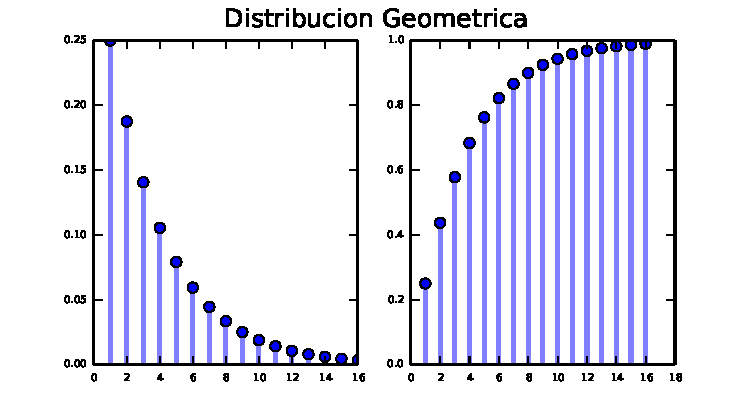
\includegraphics{curso-probabilidad-udemy_files/figure-latex/unnamed-chunk-43-1.pdf}

\hypertarget{distribuciuxf3n-binomial-negativa}{%
\subsection{Distribución binomial negativa}\label{distribuciuxf3n-binomial-negativa}}

\textbf{El problema de la puerta con dos cerraduras}

Supongamos que disponemos de 10 llaves distintas y tenemos que abrir una puerta con \textbf{dos cerraduras}.

Comenzamos por la primera cerradura, de tal forma que cada vez olvidamos qué llave hemos probado.

Una vez abierta la primera cerradura probamos de igual forma con la segunda hasta que también la abrimos.

Sea \(X\) la v.a. que cuenta el número de fracasos hasta abrir la puerta.

Acertar una llave de la puerta es un experimento Bernoulli con probabilidad de éxito \(p=0.1\). Lo repetiremos hasta obtener 2 éxitos.

En general, tendremos un experimento de Bernoulli con probabilidad de éxito \(0<p<1\) tal que:

\begin{itemize}
\tightlist
\item
  Repetimos el experimento hasta obtener el \(n\)-ésimo éxito ¡¡abrir la maldita puerta!!.
\item
  Sea \(X\) la v.a. que cuenta el número fallos hasta abrir la puerta, es decir, hasta conseguir el \(n\)-ésimo éxito. Notemos que no contamos los éxitos, solo contamos los fracasos.
\end{itemize}

Si representamos como es habitual un suceso como una cadena de F's y E's, para \(n=2\), algunos sucesos elementales serán:
\[\{EE,FEE,EFE, FFEE,FEFE,EFFE,FFFEE,FFEFE,FEFFE,EFFFE\}.\]

Calculemos algunas probabilidades para \(n=2\):
\[
\begin{array}{rl}
P(X=0) & =P(\{EE\})=p^2, \\
P(X=1) & =P(\{FEE,EFE\})=2\cdot (1-p)\cdot p^2, \\
P(X=2) & =P(\{FFEE,FEFE,EFFE\})=3\cdot (1-p) 2\cdot p^2, \\
P(X=3) & =P(\{FFFEE,FFEFE,FEFFE,EFFFE\})=4\cdot (1-p)^3\cdot p^2.
\end{array}
\]
En general su función de probabilidad es
\[
P_{X}(k)=P(X=k)=\left\{\begin{array}{ll}
     {{k+n-1}\choose{n-1}} \cdot (1-p)^{k}\cdot p^n, & \mbox{si } k=0,1,\ldots\\
     0, & \mbox{en otro caso.}\end{array}\right.
\]

Una v.a. con este tipo de distribución recibe el nombre de \textbf{binomial negativa} y la denotaremos por \(BN(n,p)\).

Notemos que \(BN(1,p)=Ge(p)\).

\textbf{Demostración}

Justifiquemos el resultado. Sea \(X\) una \(BN(n,p)\) y sea \(k=0,1,2,\ldots\)

\[P(X=k)=P(\mbox{Todas las cadenas de E's y F' con $k$ F, con $n$ E y acabadas en E})\]

\[
\overbrace{\underbrace{\overbrace{EFFF\ldots EEF}^{n-1 \quad \mbox{Éxitos}.}}}_{k \quad\mbox{Fracasos}}^{k+n-1\mbox{ posiciones}}E
\]

De estas cadenas hay tantas como maneras de elegir de entre las \(k+n-1\) primeras posiciones \(n-1\) para colocar los éxitos. Esta cantidad es el número binomial \({k+n-1\choose n-1}\).

\textbf{Números binomiales negativos}

Dados dos enteros positivos \(n\) y \(k\), se define el número binomial negativo como:
\[\binom{-n}{k}=\frac{(-n)(-n-1)\cdots (-n-k+1)}{k!}.\]
Los números binomiales negativos generalizan la fórmula de Newton para exponentes negativos:
\[
(t+1)^{-n}=\sum_{k=0}^{+\infty}\left(\begin{array}{c} -n
\\ k\end{array}\right) t^{k}.
\]

\texttt{R} usa la función \texttt{choose} para calcular números binomiales, sean negativos o no. Veámoslo con un ejemplo:
\[
{-6\choose 4}=\frac{-6\cdot (-6-1)\cdot \cdot (-6-2)\cdot (-6-3) }{4!}= \frac{-6\cdot(-7)\cdot (-8)\cdot (-9)}{24}
= \frac{3024}{24}=126.
\]
Si realizamos el cálculo con \texttt{R} obtenemos el mismo resultado:

\begin{Shaded}
\begin{Highlighting}[]
\KeywordTok{choose}\NormalTok{(}\OperatorTok{-}\DecValTok{6}\NormalTok{,}\DecValTok{4}\NormalTok{)}
\end{Highlighting}
\end{Shaded}

\begin{verbatim}
## [1] 126
\end{verbatim}

\textbf{Esperanza de una \(BN(n,p)\)}

Su \textbf{esperanza es}:

\[E(X)=\sum_{k=0}^{+\infty} k\cdot {k+n-1\choose n-1} \cdot (1-p)^{k}\cdot p^n=n\cdot\frac{1-p}{p}.\]

La \textbf{esperanza de \(X^2\)} es:

\[E(X^2)=\sum_{k=0}^{+\infty} k^2\cdot {k+n-1\choose n-1} \cdot (1-p)^{k}\cdot p^n=n\cdot\frac{1-p}{p^2}+\left(n\cdot \frac{1-p}{p}\right)^2.\]

\textbf{Varianza de una \(BN(n,p)\)}

Por último, la \textbf{varianza} es:
\[
Var(X)=E(X^2)-E(X)^2=n\cdot \frac{1-p}{p^2}+\left(n\cdot \frac{1-p}{p}\right)^2-\left(n\cdot \frac{1-p}{p}\right)^2=
n\cdot \frac{1-p}{p^2},
\]
y la desviación típica es:

\[\sqrt{Var(X)} = \frac{\sqrt{n(1-p)}}{p}.\]

\textbf{Resumen Binomial Negativa \(BN(n,p)\)}

\begin{longtable}[]{@{}rl@{}}
\toprule
\begin{minipage}[b]{0.50\columnwidth}\raggedleft
\(X\), \(BN(n,p)\)\strut
\end{minipage} & \begin{minipage}[b]{0.44\columnwidth}\raggedright
Número de fracasos antes de conseguir el \(n\)-ésimo éxito. Probabilidad de éxito \(p\)\strut
\end{minipage}\tabularnewline
\midrule
\endhead
\begin{minipage}[t]{0.50\columnwidth}\raggedleft
\(D_X=\)\strut
\end{minipage} & \begin{minipage}[t]{0.44\columnwidth}\raggedright
\(\{0,1,2,3\ldots\}\)\strut
\end{minipage}\tabularnewline
\begin{minipage}[t]{0.50\columnwidth}\raggedleft
\(P_X(k)=P(X=k)=\)\strut
\end{minipage} & \begin{minipage}[t]{0.44\columnwidth}\raggedright
\(\left\{\begin{array}{ll} {k+n-1\choose n-1} \cdot (1-p)^{k}\cdot p^n, & \mbox{si } k=0,1,\ldots \\ 0, & \mbox{en otro caso.}\end{array}\right.\)\strut
\end{minipage}\tabularnewline
\begin{minipage}[t]{0.50\columnwidth}\raggedleft
\(F_X(x)=P(X\leq x)=\)\strut
\end{minipage} & \begin{minipage}[t]{0.44\columnwidth}\raggedright
\(\begin{array}{l}\left\{\begin{array}{ll} 0, & \mbox{si } x<0\\\displaystyle\sum_{i=0}^{k} P(X=i) & \mbox{si }\left\{\begin{array}{l}k\leq x< k+1,\\k=0,1,2,\ldots\end{array}\right.\end{array}\right. \\\mbox{Calcular la suma o utilizar funciones de `R` o python.} \end{array}\)\strut
\end{minipage}\tabularnewline
\begin{minipage}[t]{0.50\columnwidth}\raggedleft
\(E(X)=n\cdot\frac{1-p}{p}\)\strut
\end{minipage} & \begin{minipage}[t]{0.44\columnwidth}\raggedright
\(Var(X)=n\cdot \frac{1-p}{p^2}\)\strut
\end{minipage}\tabularnewline
\bottomrule
\end{longtable}

\textbf{Ejercicio: Puerta con dos cerraduras}

Recordemos nuestra puerta con dos cerraduras que se abren secuencialmente. Tenemos un manojo de 10 llaves casi idénticas de manera que cada vez que probamos una llave olvidamos qué llave hemos usado.

Sea \(X\) la v.a que nos da el número de intentos fallidos hasta abrir abrir la puerta.

Estamos interesado en modelar este problema. La preguntas son:

\begin{enumerate}
\def\labelenumi{\arabic{enumi}.}
\tightlist
\item
  ¿Cuál es la distribución de probabilidad de \(X\) la v.a que nos da el número fallos hasta abrir la puerta?
\item
  ¿Cuál es la función de probabilidad y de distribución del \(X\)?
\item
  ¿Cuál es la probabilidad de fallar exactamente 5 veces antes de abrir la puerta?
\item
  ¿Cuál es la probabilidad de fallar más de 4?
\item
  ¿Cuál es el número esperado de fallos? ¿Y su desviación típica?
\end{enumerate}

\textbf{Solución 1.} ¿Cuál es la distribución de probabilidad de \(X\) la v.a que nos da el número fallos hasta abrir la puerta?

Bajo estados condiciones tenemos que la probabilidad de ``éxito'' de cada intento es \(p=\frac{1}{10}=0.1\). Como cada vez \emph{olvidamos} qué llave hemos probado, cada intento será independiente del anterior.

Así que la variable \(X\) que queremos modelar cuenta el número de fallos de repeticiones sucesivas e independientes de un experimento \(Ber(p=0.1)\) hasta conseguir 2 éxitos en un experimento.

Por lo tanto podemos asegurar que \(X\) sigue un distribución \(BN(n=2,p=0.1).\)

\textbf{Solución 2.} ¿Cuál es la función de probabilidad y de distribución del \(X\)?

En general la función de probabilidad de una \(BN(n,p)\) es

\[
P_X(X=k)=
\left\{
\begin{array}{cc} 
{k+n-1\choose n-1} \cdot (1-p)^{k}\cdot p^n, & \mbox{si }  k=0,1,\ldots \\ 0, & \mbox{en otro caso.}\end{array}\right.
\]
Si aplicamos la expresión anterior para \(n=2\) y \(p=0.1\), obtenemos:

\[
P_X(X=k)=
\left\{
\begin{array}{cc} 
{k+2-1\choose 2-1} \cdot 0.9^{k}\cdot 0.1^2, & \mbox{si }  k=0,1,2,\ldots \\ 0, & \mbox{en otro caso.}\end{array}\right.
\]
Simplificando,
\[
P_X(X=k)=P(X=k)=
\left\{
\begin{array}{cc} 
0.01\cdot (k+1)\cdot 0.9^{k}, & \mbox{si }  k=0,1,2,\ldots \\ 0 & \mbox{en otro caso.}\end{array}\right.
\]
La función de distribución en general es

\[
F_X(x)=P(X\leq x)=
\left\{
\begin{array}{ll}
0, & \mbox{si } x<0, \\
\displaystyle\sum_{i=0}^{k }{i+n-1\choose n-1} \cdot (1-p)^{i+n-1}\cdot p^n, 
& \mbox{si }\left\{\begin{array}{l} k\leq x< k+1,\\k=0,1,2,\ldots\end{array}\right. 
\end{array}
\right.
\]
Simplificando para \(n=2\), \(p=0.1\).

\[
F_X(x)=P(X\leq x)=
\left\{
\begin{array}{ll}
0, & \mbox{si } x<0, \\
\displaystyle\sum_{i=0}^{k }0.01\cdot (i+1) \cdot 0.9^{i+1},
& \mbox{si }\left\{\begin{array}{l} k\leq x< k+1,\\k=0,1,2,\ldots\end{array}\right. 
\end{array}
\right.
\]

\textbf{Solución 3.} ¿Cuál es la probabilidad de fallar exactamente 5 veces antes de abrir la puerta?
\[
P(X=5)= 0.01\cdot (5+1) \cdot 0.9^{5}= 0.06 \cdot 0.9^{5}= 0.0354294.
\]

\textbf{Solución 4.} ¿Cuál es la probabilidad de fallar más de 4?

Nos piden calcular \(P(X>4)=1-P(X\leq 4).\)

Calculemos primero \(P(X\leq 4):\)

\[
\begin{array}{rl}
P(X\leq 4) &=  \displaystyle\sum_{x=0}^{4} P(X=x) \\ & =P(X=0)+P(X=1)+P(X=2)+P(X=3)+P(X=4)\\
&= 0.01\cdot (0+1) \cdot 0.9^{0}+0.01\cdot (1+1) \cdot 0.9^{1}+0.01\cdot (2+1) \cdot 0.9^{2} \\ &\ \ 
+0.01\cdot (3+1) \cdot 0.9^{3} + 0.01\cdot (4+1) \cdot 0.9^{4} \\ & =
0.01 +0.018+0.0243+0.02916+0.032805 = 0.114265.
\end{array}
\]

Por lo tanto

\[
P(X>4)=1-P(X\leq 4)=1-0.114265=
0.885735.
\]

\textbf{Solución 5.} ¿Cuál es el número esperado de fallos? ¿Y su desviación típica?

Como \(X\) sigue una ley \(BN(n=2,p=0.1)\)

\[E(X)=n\cdot \frac{1-p}{p}=2\cdot \frac{1-0.1}{0.1}=18.\]

El número de fallos esperado es 18.

La varianza será:
\[
Var(X)=n\cdot\frac{1-p}{p^2}=2 \cdot \frac{1-0.1}{0.1^2}=180.
\]
La varianza de \(X\) es 180 y su desviación típica \(\sqrt{180}=13.41641.\)

\textbf{Cálculos con \texttt{R}}

La función de \texttt{R} que calcula la función de probabilidad de la binomial negativa con sus parámetros básicos es:

\begin{verbatim}
dnbinom(x, size, prob,...)`
\end{verbatim}

donde \texttt{size} (\(n\)) es el número de éxitos y \texttt{prob} (\(p\)), la probabilidad de éxito.

Así en el ejemplo de la puerta con dos cerraduras, \(X\) es una \(BN(n=size=2,p=prob=0.1)\). Por ejemplo, \(P(X=5)\) que hemos calculado en el ejemplo anterior, vale:

\begin{Shaded}
\begin{Highlighting}[]
\KeywordTok{dnbinom}\NormalTok{(}\DecValTok{5}\NormalTok{,}\DataTypeTok{size=}\DecValTok{2}\NormalTok{,}\DataTypeTok{p=}\FloatTok{0.1}\NormalTok{)}
\end{Highlighting}
\end{Shaded}

\begin{verbatim}
## [1] 0.0354294
\end{verbatim}

De forma similar calculamos calculamos \(P(X\leq 4)\), \(P(X>4)=1-P(X\leq 4)\) y \(P(X>4)\).

\begin{Shaded}
\begin{Highlighting}[]
\KeywordTok{pnbinom}\NormalTok{(}\DecValTok{4}\NormalTok{,}\DataTypeTok{size=}\DecValTok{2}\NormalTok{,}\DataTypeTok{p=}\FloatTok{0.1}\NormalTok{)}
\end{Highlighting}
\end{Shaded}

\begin{verbatim}
## [1] 0.114265
\end{verbatim}

\begin{Shaded}
\begin{Highlighting}[]
\DecValTok{1}\OperatorTok{-}\KeywordTok{pnbinom}\NormalTok{(}\DecValTok{4}\NormalTok{,}\DataTypeTok{size=}\DecValTok{2}\NormalTok{,}\DataTypeTok{p=}\FloatTok{0.1}\NormalTok{)}
\end{Highlighting}
\end{Shaded}

\begin{verbatim}
## [1] 0.885735
\end{verbatim}

\begin{Shaded}
\begin{Highlighting}[]
\KeywordTok{pnbinom}\NormalTok{(}\DecValTok{4}\NormalTok{,}\DataTypeTok{size=}\DecValTok{2}\NormalTok{,}\DataTypeTok{p=}\FloatTok{0.1}\NormalTok{,}\DataTypeTok{lower.tail=}\OtherTok{FALSE}\NormalTok{)}
\end{Highlighting}
\end{Shaded}

\begin{verbatim}
## [1] 0.885735
\end{verbatim}

\textbf{Cálculos con python}

La función con python es \texttt{nbinom.pmf(k,\ n,\ p,\ loc)}. Hay que cargarla desde \texttt{scpi.stats}

\begin{Shaded}
\begin{Highlighting}[]
\ImportTok{from}\NormalTok{ scipy.stats }\ImportTok{import}\NormalTok{ nbinom}
\end{Highlighting}
\end{Shaded}

Recordemos que de nuevo se cumple que

\begin{Shaded}
\begin{Highlighting}[]
\NormalTok{nbinom.pmf(k, n, p, loc) }\OperatorTok{=}\NormalTok{ nbinom.pmf(k}\OperatorTok{-}\NormalTok{loc, n, p)`}
\end{Highlighting}
\end{Shaded}

\begin{Shaded}
\begin{Highlighting}[]
\NormalTok{nbinom.pmf(k}\OperatorTok{=}\DecValTok{5}\NormalTok{,n}\OperatorTok{=}\DecValTok{2}\NormalTok{,p}\OperatorTok{=}\FloatTok{0.1}\NormalTok{)}
\end{Highlighting}
\end{Shaded}

\begin{verbatim}
## 0.035429400000000041
\end{verbatim}

\begin{Shaded}
\begin{Highlighting}[]
\NormalTok{nbinom.pmf(k}\OperatorTok{=}\DecValTok{5}\NormalTok{,n}\OperatorTok{=}\DecValTok{2}\NormalTok{,p}\OperatorTok{=}\FloatTok{0.1}\NormalTok{,loc}\OperatorTok{=}\DecValTok{0}\NormalTok{)}
\end{Highlighting}
\end{Shaded}

\begin{verbatim}
## 0.035429400000000041
\end{verbatim}

\begin{Shaded}
\begin{Highlighting}[]
\NormalTok{nbinom.cdf(k}\OperatorTok{=}\DecValTok{4}\NormalTok{,n}\OperatorTok{=}\DecValTok{2}\NormalTok{,p}\OperatorTok{=}\FloatTok{0.1}\NormalTok{)}
\end{Highlighting}
\end{Shaded}

\begin{verbatim}
## 0.11426500000000003
\end{verbatim}

\begin{Shaded}
\begin{Highlighting}[]
\DecValTok{1}\OperatorTok{-}\NormalTok{nbinom.cdf(k}\OperatorTok{=}\DecValTok{4}\NormalTok{,n}\OperatorTok{=}\DecValTok{2}\NormalTok{,p}\OperatorTok{=}\FloatTok{0.1}\NormalTok{)}
\end{Highlighting}
\end{Shaded}

\begin{verbatim}
## 0.88573499999999994
\end{verbatim}

Generemos 100 observaciones aleatorias de una \(BN(n=2,0.1)\). Es decir serán las veces que hemos fallado hasta abrir la puerta 100 veces.

\begin{Shaded}
\begin{Highlighting}[]
\NormalTok{nbinom.rvs(n}\OperatorTok{=}\DecValTok{2}\NormalTok{, p}\OperatorTok{=}\FloatTok{0.1}\NormalTok{, size}\OperatorTok{=}\DecValTok{100}\NormalTok{)}
\end{Highlighting}
\end{Shaded}

\begin{verbatim}
## array([14,  2, 11, 17, 43, 15,  8, 46,  5, 12, 33,  8, 26,  9, 15, 27, 13,
##        23, 18, 28,  5, 11,  1, 18, 30, 25, 40,  3, 18, 35,  6, 23, 18, 32,
##        24, 18, 39, 11, 34,  7, 35, 22,  4, 25, 13, 15,  8, 28, 20,  8, 12,
##        41, 17,  8, 16,  5, 12, 11, 17,  0, 22, 10, 43, 18, 20, 32, 12, 21,
##        22, 17,  8,  8, 20, 32, 49, 22, 19, 17,  2,  7,  7, 19, 12, 15, 11,
##        26, 30,  0, 48,  9,  6, 10,  3, 13, 34,  8, 19,  7, 37, 12])
\end{verbatim}

La \textbf{esperanza} y la \textbf{varianza}de una \(BN(n=2,0.1)\) valen:

\begin{Shaded}
\begin{Highlighting}[]
\NormalTok{n, p}\OperatorTok{=}\DecValTok{2}\NormalTok{,}\FloatTok{0.1}
\NormalTok{params }\OperatorTok{=}\NormalTok{ nbinom.stats(n,p,moments}\OperatorTok{=}\StringTok{'mv'}\NormalTok{)}
\BuiltInTok{print}\NormalTok{(}\StringTok{"E(X)=}\SpecialCharTok{\{m\}}\StringTok{"}\NormalTok{.}\BuiltInTok{format}\NormalTok{(m}\OperatorTok{=}\NormalTok{params[}\DecValTok{0}\NormalTok{]))}
\end{Highlighting}
\end{Shaded}

\begin{verbatim}
## E(X)=18.0
\end{verbatim}

\begin{Shaded}
\begin{Highlighting}[]
\BuiltInTok{print}\NormalTok{(}\StringTok{"Var(X)=}\SpecialCharTok{\{v\}}\StringTok{"}\NormalTok{.}\BuiltInTok{format}\NormalTok{(v}\OperatorTok{=}\NormalTok{params[}\DecValTok{1}\NormalTok{]))}
\end{Highlighting}
\end{Shaded}

\begin{verbatim}
## Var(X)=180.0
\end{verbatim}

\textbf{Gráficas de la binomial negativa con \texttt{R}}

El siguiente código de \texttt{R} dibuja las función de probabilidad y la de distribución de una \(BN(n=2,p=0.1)\)

\begin{Shaded}
\begin{Highlighting}[]
\KeywordTok{par}\NormalTok{(}\DataTypeTok{mfrow=}\KeywordTok{c}\NormalTok{(}\DecValTok{1}\NormalTok{,}\DecValTok{2}\NormalTok{))}
\NormalTok{aux=}\KeywordTok{rep}\NormalTok{(}\DecValTok{0}\NormalTok{,}\DecValTok{22}\NormalTok{)}
\NormalTok{aux[}\KeywordTok{seq}\NormalTok{(}\DecValTok{2}\NormalTok{,}\DecValTok{22}\NormalTok{,}\DecValTok{2}\NormalTok{)]=}\KeywordTok{dnbinom}\NormalTok{(}\KeywordTok{c}\NormalTok{(}\DecValTok{0}\OperatorTok{:}\DecValTok{10}\NormalTok{),}\DataTypeTok{size=}\DecValTok{2}\NormalTok{,}\DataTypeTok{prob=}\FloatTok{0.1}\NormalTok{)}
\KeywordTok{plot}\NormalTok{(}\DataTypeTok{x=}\KeywordTok{c}\NormalTok{(}\DecValTok{0}\OperatorTok{:}\DecValTok{10}\NormalTok{),}\DataTypeTok{y=}\KeywordTok{dnbinom}\NormalTok{(}\KeywordTok{c}\NormalTok{(}\DecValTok{0}\OperatorTok{:}\DecValTok{10}\NormalTok{),}\DataTypeTok{size=}\DecValTok{2}\NormalTok{,}\DataTypeTok{prob=}\FloatTok{0.1}\NormalTok{),}
  \DataTypeTok{ylim=}\KeywordTok{c}\NormalTok{(}\DecValTok{0}\NormalTok{,}\DecValTok{1}\NormalTok{),}\DataTypeTok{xlim=}\KeywordTok{c}\NormalTok{(}\OperatorTok{-}\DecValTok{1}\NormalTok{,}\DecValTok{11}\NormalTok{),}\DataTypeTok{xlab=}\StringTok{"x"}\NormalTok{,}
  \DataTypeTok{main=}\StringTok{"Función de probabilidad}\CharTok{\textbackslash{}n}\StringTok{ BN(n=2,p=0.1)"}\NormalTok{)}
\KeywordTok{lines}\NormalTok{(}\DataTypeTok{x=}\KeywordTok{rep}\NormalTok{(}\DecValTok{0}\OperatorTok{:}\DecValTok{10}\NormalTok{,}\DataTypeTok{each=}\DecValTok{2}\NormalTok{),}\DataTypeTok{y=}\NormalTok{aux, }\DataTypeTok{type =} \StringTok{"h"}\NormalTok{, }\DataTypeTok{lty =} \DecValTok{2}\NormalTok{,}\DataTypeTok{col=}\StringTok{"blue"}\NormalTok{)}
\KeywordTok{curve}\NormalTok{(}\KeywordTok{pnbinom}\NormalTok{(x,}\DataTypeTok{size=}\DecValTok{2}\NormalTok{,}\DataTypeTok{prob=}\DecValTok{0}\NormalTok{,}\DecValTok{1}\NormalTok{),}
  \DataTypeTok{xlim=}\KeywordTok{c}\NormalTok{(}\OperatorTok{-}\DecValTok{1}\NormalTok{,}\DecValTok{11}\NormalTok{),}\DataTypeTok{col=}\StringTok{"blue"}\NormalTok{,}
  \DataTypeTok{main=}\StringTok{"Función de distribución\textbackslash{}n BN(n=2,p=0.1)"}\NormalTok{)}
\KeywordTok{par}\NormalTok{(}\DataTypeTok{mfrow=}\KeywordTok{c}\NormalTok{(}\DecValTok{1}\NormalTok{,}\DecValTok{1}\NormalTok{))}
\end{Highlighting}
\end{Shaded}

\begin{center}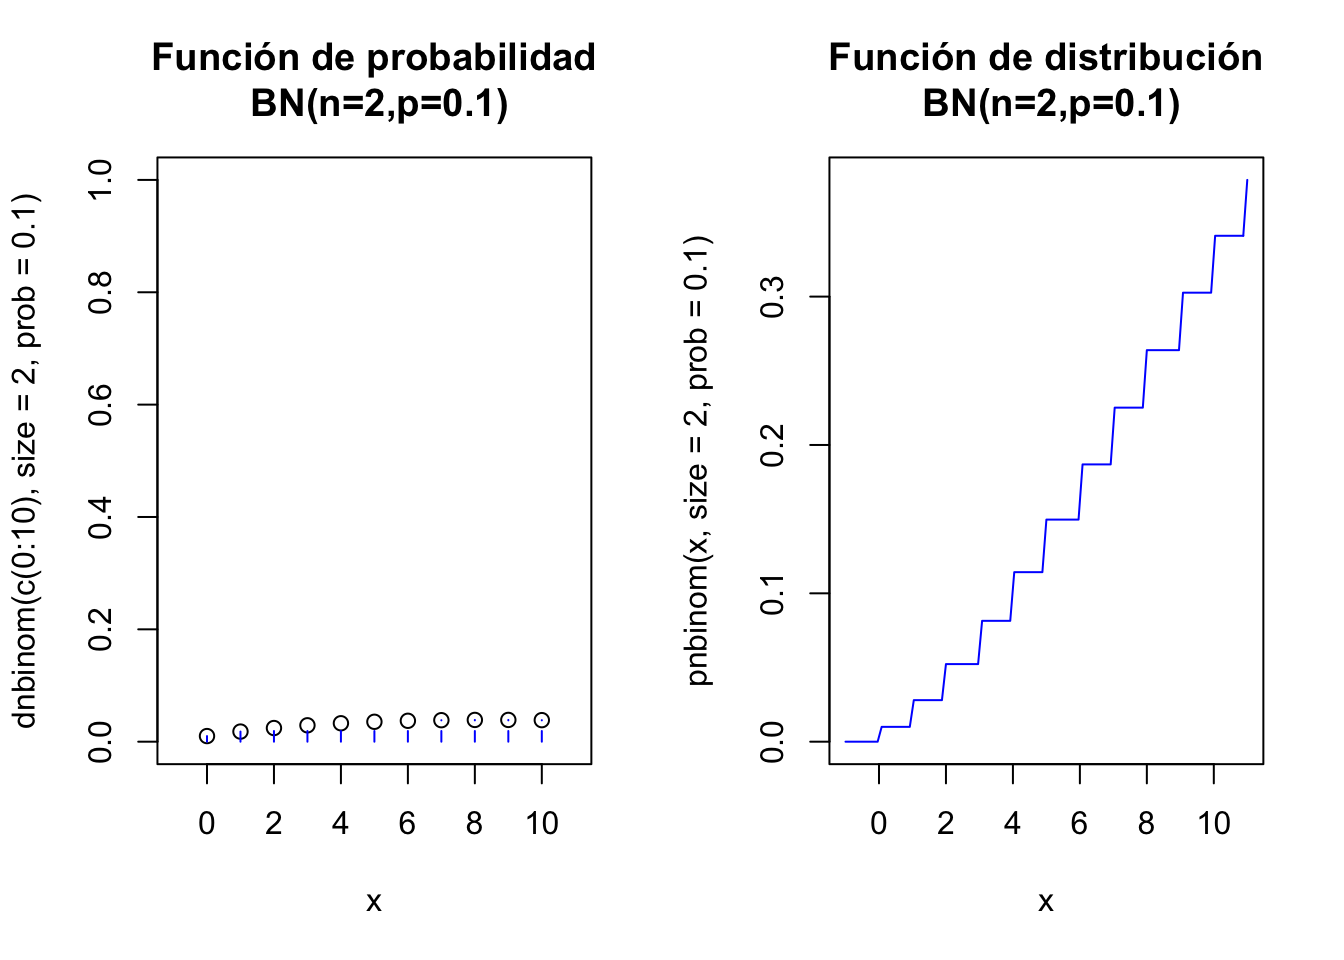
\includegraphics{curso-probabilidad-udemy_files/figure-latex/unnamed-chunk-54-1} \end{center}

\textbf{Gráficas interactivas binomial negativa}

Para ejecutar el siguiente gráfico interactivo, solamente tienes que cargar el paquete \texttt{shiny} en tu ordenador y luego copiar/pegar las siguientes instrucciones. De este modo podrás observar los cambios en las distribuciones variando los parámetros.

\begin{Shaded}
\begin{Highlighting}[]
\KeywordTok{fluidPage}\NormalTok{(}
\KeywordTok{fluidRow}\NormalTok{(}
  \KeywordTok{column}\NormalTok{(}\DecValTok{6}\NormalTok{,}
         \KeywordTok{sliderInput}\NormalTok{(}\StringTok{"n_nbinom"}\NormalTok{, }\DataTypeTok{label =} \StringTok{"Número de éxitos n:"}\NormalTok{,}
              \DataTypeTok{min =} \DecValTok{1}\NormalTok{, }\DataTypeTok{max =} \DecValTok{50}\NormalTok{, }\DataTypeTok{value =}\DecValTok{20}\NormalTok{ , }\DataTypeTok{step =} \DecValTok{1}\NormalTok{)),}
  \KeywordTok{column}\NormalTok{(}\DecValTok{6}\NormalTok{,}
          \KeywordTok{sliderInput}\NormalTok{(}\StringTok{"p_nbinom"}\NormalTok{, }\DataTypeTok{label =} \StringTok{"Probabilidad de un éxito p:"}\NormalTok{,}
                     \DataTypeTok{min =} \FloatTok{0.01}\NormalTok{, }\DataTypeTok{max =} \FloatTok{0.99}\NormalTok{, }\DataTypeTok{value =} \FloatTok{0.8}\NormalTok{, }\DataTypeTok{step =} \FloatTok{0.01}\NormalTok{)}
\NormalTok{         )}
\NormalTok{  )}
\NormalTok{)}

\KeywordTok{renderPlot}\NormalTok{(\{}
\NormalTok{  n=input}\OperatorTok{$}\NormalTok{n_nbinom}
\NormalTok{  pr=input}\OperatorTok{$}\NormalTok{p_nbinom}
  
  \KeywordTok{par}\NormalTok{(}\DataTypeTok{mfrow=}\KeywordTok{c}\NormalTok{(}\DecValTok{1}\NormalTok{,}\DecValTok{2}\NormalTok{))}
\NormalTok{  aux=}\KeywordTok{rep}\NormalTok{(}\DecValTok{0}\NormalTok{,(n}\OperatorTok{+}\DecValTok{1}\NormalTok{)}\OperatorTok{*}\DecValTok{2}\NormalTok{)}
\NormalTok{  aux[}\KeywordTok{seq}\NormalTok{(}\DecValTok{2}\NormalTok{,(n}\OperatorTok{+}\DecValTok{1}\NormalTok{)}\OperatorTok{*}\DecValTok{2}\NormalTok{,}\DecValTok{2}\NormalTok{)]=}\KeywordTok{dnbinom}\NormalTok{(}\KeywordTok{c}\NormalTok{(}\DecValTok{0}\OperatorTok{:}\NormalTok{n),}\DataTypeTok{size=}\NormalTok{n,}\DataTypeTok{prob=}\NormalTok{pr)}
  \KeywordTok{plot}\NormalTok{(}\DataTypeTok{x=}\KeywordTok{c}\NormalTok{(}\DecValTok{0}\OperatorTok{:}\NormalTok{n),}\DataTypeTok{y=}\KeywordTok{dnbinom}\NormalTok{(}\KeywordTok{c}\NormalTok{(}\DecValTok{0}\OperatorTok{:}\NormalTok{n),}\DataTypeTok{size=}\NormalTok{n,}\DataTypeTok{prob=}\NormalTok{pr),}
       \DataTypeTok{ylim=}\KeywordTok{c}\NormalTok{(}\DecValTok{0}\NormalTok{,}\DecValTok{1}\NormalTok{),}\DataTypeTok{xlim=}\KeywordTok{c}\NormalTok{(}\OperatorTok{-}\DecValTok{1}\NormalTok{,n}\OperatorTok{+}\DecValTok{1}\NormalTok{),}\DataTypeTok{xlab=}\StringTok{"x"}\NormalTok{,}
       \DataTypeTok{main=}\KeywordTok{paste0}\NormalTok{(}\KeywordTok{c}\NormalTok{(}\StringTok{"Función de probabilidad}\CharTok{\textbackslash{}n}\StringTok{ BN(n="}\NormalTok{,n,}\StringTok{",p="}\NormalTok{,pr,}\StringTok{")"}\NormalTok{),}\DataTypeTok{collapse =} \StringTok{""}\NormalTok{))}
  \KeywordTok{lines}\NormalTok{(}\DataTypeTok{x=}\KeywordTok{rep}\NormalTok{(}\DecValTok{0}\OperatorTok{:}\NormalTok{n,}\DataTypeTok{each=}\DecValTok{2}\NormalTok{),}\DataTypeTok{y=}\NormalTok{aux, }\DataTypeTok{type =} \StringTok{"h"}\NormalTok{, }\DataTypeTok{lty =} \DecValTok{2}\NormalTok{,}\DataTypeTok{col=}\StringTok{"blue"}\NormalTok{)}
  \KeywordTok{curve}\NormalTok{(}\KeywordTok{pnbinom}\NormalTok{(x,}\DataTypeTok{size=}\NormalTok{n,}\DataTypeTok{p=}\NormalTok{pr),}
        \DataTypeTok{xlim=}\KeywordTok{c}\NormalTok{(}\OperatorTok{-}\DecValTok{1}\NormalTok{,n}\OperatorTok{+}\DecValTok{1}\NormalTok{),}\DataTypeTok{col=}\StringTok{"blue"}\NormalTok{,}
        \DataTypeTok{main=}\KeywordTok{paste0}\NormalTok{(}\KeywordTok{c}\NormalTok{(}\StringTok{"Función de distribución\textbackslash{}n BN(n="}\NormalTok{,n,}\StringTok{",p="}\NormalTok{,pr,}\StringTok{")"}\NormalTok{),}
                    \DataTypeTok{collapse =} \StringTok{""}\NormalTok{))}
  \KeywordTok{par}\NormalTok{(}\DataTypeTok{mfrow=}\KeywordTok{c}\NormalTok{(}\DecValTok{1}\NormalTok{,}\DecValTok{1}\NormalTok{))}
\NormalTok{\})}
\end{Highlighting}
\end{Shaded}

\textbf{Ejercicio}

Buscad en los manuales de python cómo se dibuja la función de probabilidad y de distribución de una binomial.
negativa

Necesitamos de nuevo más librerías

\begin{Shaded}
\begin{Highlighting}[]
\ImportTok{import}\NormalTok{ numpy }\ImportTok{as}\NormalTok{ np}
\ImportTok{from}\NormalTok{ scipy.stats }\ImportTok{import}\NormalTok{ nbinom}
\ImportTok{import}\NormalTok{ matplotlib.pyplot }\ImportTok{as}\NormalTok{ plt}
\end{Highlighting}
\end{Shaded}

\begin{Shaded}
\begin{Highlighting}[]
\NormalTok{n, p }\OperatorTok{=} \DecValTok{10}\NormalTok{, }\FloatTok{0.25}
\NormalTok{x }\OperatorTok{=}\NormalTok{ np.arange(}\DecValTok{0}\NormalTok{,nbinom.ppf(}\FloatTok{0.99}\NormalTok{, n, p))}
\NormalTok{fig }\OperatorTok{=}\NormalTok{plt.figure(figsize}\OperatorTok{=}\NormalTok{(}\DecValTok{5}\NormalTok{, }\FloatTok{2.7}\NormalTok{))}
\NormalTok{ax }\OperatorTok{=}\NormalTok{ fig.add_subplot(}\DecValTok{1}\NormalTok{,}\DecValTok{2}\NormalTok{,}\DecValTok{1}\NormalTok{)}
\NormalTok{ax.plot(x, nbinom.pmf(x, n, p), }\StringTok{'bo'}\NormalTok{, ms}\OperatorTok{=}\DecValTok{5}\NormalTok{, label}\OperatorTok{=}\StringTok{'nbinom pmf'}\NormalTok{)}
\NormalTok{ax.vlines(x, }\DecValTok{0}\NormalTok{, nbinom.pmf(x, n, p), colors}\OperatorTok{=}\StringTok{'b'}\NormalTok{, lw}\OperatorTok{=}\DecValTok{2}\NormalTok{, alpha}\OperatorTok{=}\FloatTok{0.5}\NormalTok{)}
\ControlFlowTok{for}\NormalTok{ tick }\KeywordTok{in}\NormalTok{ ax.xaxis.get_major_ticks():}
\NormalTok{  tick.label.set_fontsize(}\DecValTok{5}\NormalTok{)}
\ControlFlowTok{for}\NormalTok{ tick }\KeywordTok{in}\NormalTok{ ax.yaxis.get_major_ticks():}
\NormalTok{  tick.label.set_fontsize(}\DecValTok{5}\NormalTok{) }
\NormalTok{ax }\OperatorTok{=}\NormalTok{ fig.add_subplot(}\DecValTok{1}\NormalTok{,}\DecValTok{2}\NormalTok{,}\DecValTok{2}\NormalTok{)}
\NormalTok{ax.plot(x, nbinom.cdf(x, n, p), }\StringTok{'bo'}\NormalTok{, ms}\OperatorTok{=}\DecValTok{5}\NormalTok{, label}\OperatorTok{=}\StringTok{'nbinom pmf'}\NormalTok{)}
\NormalTok{ax.vlines(x, }\DecValTok{0}\NormalTok{, nbinom.cdf(x, n, p), colors}\OperatorTok{=}\StringTok{'b'}\NormalTok{, lw}\OperatorTok{=}\DecValTok{2}\NormalTok{, alpha}\OperatorTok{=}\FloatTok{0.5}\NormalTok{)}
\ControlFlowTok{for}\NormalTok{ tick }\KeywordTok{in}\NormalTok{ ax.xaxis.get_major_ticks():}
\NormalTok{  tick.label.set_fontsize(}\DecValTok{5}\NormalTok{)}
\ControlFlowTok{for}\NormalTok{ tick }\KeywordTok{in}\NormalTok{ ax.yaxis.get_major_ticks():}
\NormalTok{  tick.label.set_fontsize(}\DecValTok{5}\NormalTok{)}
\NormalTok{fig.suptitle(}\StringTok{'Distribucion Binomial Negativa'}\NormalTok{)}
\NormalTok{plt.show()}
\end{Highlighting}
\end{Shaded}

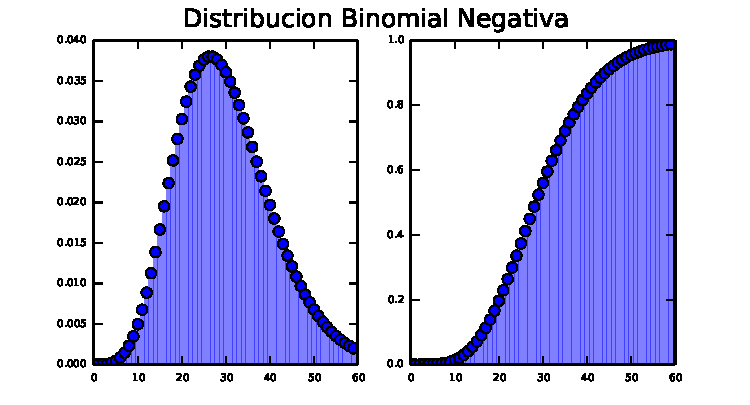
\includegraphics{curso-probabilidad-udemy_files/figure-latex/negativa_py_show-1.pdf}

\textbf{Ejercicio: acceso aleatorio a un sistema con triple clave}

Supongamos que tenemos un sistema informático tiene un programa de seguridad que genera accesos con claves de 3 dígitos \(000,001,\ldots 999\). En total tenemos 1000 posibilidades.

Como una clave de tres dígitos es fácil de romper proponemos considerar tres claves consecutivas de acceso al sistema, cada una de 3 dígitos.

Para acceder al sistema hay que dar las tres claves de forma consecutiva y por orden.

Es decir hasta que no averiguamos la primera clave no pasamos a la segunda clave.

Supongamos que cada vez que ponemos las dos claves olvidamos el resultado y seguimos poniendo claves al azar hasta adivinar la contraseña.

Así hasta conseguir entrar en el sistema.

Sea \(X\) la v.a que nos da el número de fallos antes de entrar en el sistema.

Estamos interesados en modelar este problema. La preguntas son:

\begin{enumerate}
\def\labelenumi{\arabic{enumi}.}
\tightlist
\item
  ¿Cuál es la distribución de probabilidad de \(X\), la v.a que nos da el número de fallos antes de acceder al sistema.
\item
  ¿Cuál es la función de probabilidad y de distribución del \(X\)?
\item
  ¿Cuál es la probabilidad de fallar 150 veces antes de acceder en el sistema?
\item
  ¿Cuál es la probabilidad de fallar más de 150 veces antes de entrar en el sistema?
\item
  ¿Cuál es el número esperado de fallos antes de acceder al sistema? ¿Y su varianza?
\end{enumerate}

\textbf{Solución 1.} ¿Cuál es la distribución de probabilidad de \(X\), la v.a que nos da el número de fallos antes de acceder al sistema?

Bajo estados condiciones tenemos que la probabilidad de ``éxito'' de cada intento es \(p=\frac{1}{1000}=0.001\). Y como cada vez \emph{olvidamos} en los dígitos cada intento será independiente del anterior.

Así que la variable \(X\) cuenta el número de fracasos independientes hasta conseguir 3 éxitos en un experimento \(Ber(p=0.001)\) por lo tanto \(X\) sigue un distribución \(BN(n=3,p=0.001).\)

\textbf{Solución 2.} ¿Cuál es la función de probabilidad y de distribución del \(X\)

En general la función de probabilidad de una \(BN(n,p)\) es:

\[
P_X(X=x)=P(X=x)=
\left\{
\begin{array}{cc} 
{x+n-1\choose n-1} \cdot (1-p)^{x}\cdot p^n, & \mbox{si }  x=0,1,\ldots \\ 0, & \mbox{en otro caso.}\end{array}\right.
\]
En particular la función de probabilidad de una \(BN(n=3,p=0.001)\) es

\[
P_X(X=x)=P(X=x)=
\left\{
\begin{array}{cc} 
{x+2\choose 2} \cdot 0.999^{x}\cdot 0.001^3 & \mbox{si }  x=0,1,2,\ldots \\ 0 & \mbox{en otro caso.}\end{array}\right.
\]

\textbf{Solución 3.} ¿Cuál es la probabilidad de fallar 150 veces antes de acceder en el sistema?

Nos piden calcular la probabilidad siguiente:
\[
P(X=150)= {152\choose 2} \cdot 0.999^{150}\cdot 0.001^3.
\]
Realizaremos el cálculo anterior con ayuda de \texttt{R}:

\begin{Shaded}
\begin{Highlighting}[]
\KeywordTok{choose}\NormalTok{(}\DecValTok{152}\NormalTok{,}\DecValTok{2}\NormalTok{)}\OperatorTok{*}\FloatTok{0.999}\OperatorTok{^}\DecValTok{150}\OperatorTok{*}\FloatTok{0.001}\OperatorTok{^}\DecValTok{3}
\end{Highlighting}
\end{Shaded}

\begin{verbatim}
## [1] 9.876743e-06
\end{verbatim}

o, usando la función de \texttt{R} que nos calcula la función de probabilidad:

\begin{Shaded}
\begin{Highlighting}[]
\KeywordTok{dnbinom}\NormalTok{(}\DecValTok{150}\NormalTok{,}\DataTypeTok{size=}\DecValTok{3}\NormalTok{,}\DataTypeTok{p=}\FloatTok{0.001}\NormalTok{)}
\end{Highlighting}
\end{Shaded}

\begin{verbatim}
## [1] 9.876743e-06
\end{verbatim}

Si queremos calcular la probabilidad anterior con python, tenemos que hacer:

\begin{Shaded}
\begin{Highlighting}[]
\ImportTok{from}\NormalTok{  scipy.special }\ImportTok{import}\NormalTok{ binom}
\NormalTok{binom(}\DecValTok{152}\NormalTok{,}\DecValTok{2}\NormalTok{)}\OperatorTok{*}\FloatTok{0.999}\OperatorTok{**}\DecValTok{150}\OperatorTok{*}\FloatTok{0.001}\OperatorTok{**}\DecValTok{3}
\end{Highlighting}
\end{Shaded}

\begin{verbatim}
## 9.8767434596705257e-06
\end{verbatim}

\begin{Shaded}
\begin{Highlighting}[]
\NormalTok{nbinom.pmf(}\DecValTok{150}\NormalTok{,n}\OperatorTok{=}\DecValTok{3}\NormalTok{,p}\OperatorTok{=}\FloatTok{0.001}\NormalTok{)}
\end{Highlighting}
\end{Shaded}

\begin{verbatim}
## 9.8767434596702174e-06
\end{verbatim}

Vemos que es muy improbable fallar 150 veces antes de acceder al sistema.

\textbf{Solución 4.} ¿Cuál es la probabilidad de fallar más de 150 veces antes de entrar en el sistema?

Nos piden calcular la probabilidad siguiente:
\[P(X>150)=1-P(X\leq 150).\]

Calculemos \(P(X\leq 150)\)
\[
\begin{array}{rl}
P(X\leq 150) &= P(X=0)+P(X=1)+P(X=2)+\ldots+P(X=150) \\ & = \sum\limits_{k=0}^{150} {k+3-1\choose 3-1} \cdot (0.999)^{k}\cdot 0.001^3= \ldots = \ensuremath{5.2320035\times 10^{-4}}
\end{array}
\]
Si hacemos el cálculo con \texttt{R}, obtenemos:

\begin{Shaded}
\begin{Highlighting}[]
\KeywordTok{pnbinom}\NormalTok{(}\DecValTok{150}\NormalTok{,}\DecValTok{3}\NormalTok{,}\FloatTok{0.001}\NormalTok{)}
\end{Highlighting}
\end{Shaded}

\begin{verbatim}
## [1] 0.0005232003
\end{verbatim}

Si lo hacemos en python, obtenemos el mismo resultado:

\begin{Shaded}
\begin{Highlighting}[]
\NormalTok{nbinom.cdf(}\DecValTok{150}\NormalTok{,n}\OperatorTok{=}\DecValTok{3}\NormalTok{,p}\OperatorTok{=}\FloatTok{0.001}\NormalTok{)}
\end{Highlighting}
\end{Shaded}

\begin{verbatim}
## 0.00052320034908240592
\end{verbatim}

El valor pedido será pues:
\[
P(X>150)=1-P(X\leq 150)=1-\ensuremath{5.2320035\times 10^{-4}}=0.9994768.
\]
Vemos que es muy probable que fallemos más de 150 veces antes de entrar en el sistema.

\textbf{Solución 5.} ¿Cuál es el número esperado de fallos antes de acceder al sistema? ¿Y su varianza?

\[E(X)=n\cdot \frac{1-p}{p}=3\cdot \frac{1- 0.001}{0.001}=2997.\]
\[Var(X)=n\cdot \frac{1-p}{p^2}=3\cdot \frac{1- 0.001^2}{0.001^2}=\ensuremath{2.997\times 10^{6}}.\]

Con python:

\begin{Shaded}
\begin{Highlighting}[]
\NormalTok{params }\OperatorTok{=}\NormalTok{ nbinom.stats(n}\OperatorTok{=}\DecValTok{3}\NormalTok{,p}\OperatorTok{=}\FloatTok{0.001}\NormalTok{,moments}\OperatorTok{=}\StringTok{'mv'}\NormalTok{)}
\BuiltInTok{print}\NormalTok{(}\StringTok{"E(X) = }\SpecialCharTok{\{m\}}\StringTok{"}\NormalTok{.}\BuiltInTok{format}\NormalTok{(m}\OperatorTok{=}\NormalTok{params[}\DecValTok{0}\NormalTok{]))}
\end{Highlighting}
\end{Shaded}

\begin{verbatim}
## E(X) = 2997.0
\end{verbatim}

\begin{Shaded}
\begin{Highlighting}[]
\BuiltInTok{print}\NormalTok{(}\StringTok{"Var(X) = }\SpecialCharTok{\{v\}}\StringTok{"}\NormalTok{.}\BuiltInTok{format}\NormalTok{(v}\OperatorTok{=}\NormalTok{params[}\DecValTok{1}\NormalTok{]))}
\end{Highlighting}
\end{Shaded}

\begin{verbatim}
## Var(X) = 2997000.0
\end{verbatim}

\textbf{¿Tres claves de tres dígitos o una de 9 dígitos?}

\textbf{Ejercicio}

Supongamos que ponemos una sola clave de 9 dígitos. Estudiemos en este caso la variable aleatoria que da el número de fallos antes de entrar en el sistema y comparemos los resultados.

Si seguimos suponiendo que cada vez ponemos la contraseña al azar pero esta vez con una clave de 9 dígitos. La probabilidad de éxito será ahora \(p=\frac{1}{10^{9}}\).

Si llamamos \(X_9\) a la variable aleatoria que nos da el número de fallos antes de entra en el sistema seguirá una distribución \(Ge(p=\frac{1}{10^9}=0.000000001)\).

Su valor esperado es

\[
E(X_9)=\frac{1-p}{p}=\frac{1-0.000000001}{0.000000001}=\ensuremath{10\times 10^{8}}.
\]

\(1000 000 000\) son 1000 millones de fallos esperados hasta abrir la puerta.

Recordemos que con tres contraseñas de 3 dígitos el valor esperado de fallos era:

\[3\cdot \frac{1-0.001}{0.001}=2997.\]

Por lo tanto, desde el punto de vista de la seguridad, es mejor una clave larga de 9 dígitos que tres cortas si escribimos las contraseñas al azar.

\hypertarget{distribuciuxf3n-de-poisson}{%
\subsection{Distribución de Poisson}\label{distribuciuxf3n-de-poisson}}

Diremos que una v.a. discreta \(X\) con \(X(\Omega)=\mathbf{N}\) tiene distribución de Poisson con parámetro \(\lambda>0\), y lo denotaremos por \(Po(\lambda)\) si su función de probabilidad es:

\[
P_{X}(x)=P(X=x)=
\left\{\begin{array}{ll}
\frac{\lambda^x}{x!} e^{-\lambda},& \mbox{ si } x=0,1,\ldots\\
0, & \mbox{en otro caso.}\end{array}\right.
\]

Usando que el desarrollo en serie de Taylor de la función exponencial es
\[
e^{\lambda}=\sum_{x=0}^{+\infty} \frac{\lambda^x}{x!},
\]
es fácil comprobar que la suma de la función de probabilidad en todos los valores del dominio de \(X\), o sea, los enteros positivos, vale 1.

Además recordemos que dado \(x\in\mathbb{R}-\{0\}\) se tiene que

\[
\lim_{n\to\infty} \left(1+\frac{x}{n}\right)^n=e^x.
\]

Usando la expresión anterior para \(x=-\lambda\), tenemos:
\[
\lim_{n\to\infty} \left(1-\frac{\lambda}{n}\right)^n=\lim_{n\to\infty} \left(1+\frac{-\lambda}{n}\right)^n=e^{-\lambda}.
\]

\textbf{La distribución de Poisson como ``límite'' de una binomial}

La distribución de Poisson (\href{https://es.wikipedia.org/wiki/Sim\%C3\%A9on_Denis_Poisson}{Siméon Denis Poisson}) aparece en el conteo de determinados eventos que se producen en un intervalo de tiempo o en el espacio.

Supongamos que nuestra variable de interés es \(X\), el número de eventos en el intervalo de tiempo \((0,t]\), como por ejemplo el número de llamadas a un \emph{call center} en una hora donde suponemos que se cumplen las siguientes condiciones:

\begin{enumerate}
\def\labelenumi{\arabic{enumi}.}
\tightlist
\item
  El número promedio de eventos en el intervalo \((0,t]\) es \(\lambda>0\).
\item
  Es posible dividir el intervalo de tiempo en un
  gran número de subintervalos (denotemos por \(n\) al número de intervalos) de forma que:

  \begin{itemize}
  \tightlist
  \item
    La probabilidad de que se produzcan dos o más eventos en un subintervalo es despreciable.
  \item
    El número de ocurrencias de eventos en un intervalo es independiente del número de ocurrencias en otro intervalo.
  \item
    La probabilidad de que un evento ocurra en un subintervalo es \(p_n=\frac{\lambda}{n}\)·
  \end{itemize}
\end{enumerate}

Bajo estas condiciones, podemos considerar que el número de eventos en el intervalo \((0,t]\) será el número de ``éxitos'' en \(n\) repeticiones independientes de un proceso Bernoulli de parámetro \(p_n\)

Entonces si \(n\to\infty\) y \(p_n\cdot n\) se mantiene igual a \(\lambda\) resulta que la función de probabilidad de \(X_n\) se puede escribir como

\[
\begin{array}{rl}
P(X_n=k)&=\left(\begin{array}{c} n\\ k\end{array}\right) \cdot p_n^k\cdot  (1-p_n)^{n-k}
\\
&= {n\choose k}\cdot \left(\frac{\lambda}{n}\right)^{k}\cdot \left(1-\frac{\lambda}{n}\right)^{n-k}\\
&=
\frac{\lambda^k}{k!}\cdot\frac{n!}{(n-k)!\cdot n^k}\cdot
\left(1-\frac{\lambda}{n}\right)^{n}\cdot \left(1-\frac{\lambda}{n}\right)^{-k}.
\end{array}
\]
Si hacemos tender \(n\) hacia \(\infty\), obtenemos:
\[
\displaystyle\lim_{n\to \infty} P(X_n=k) = \lim_{n\to \infty} \frac{\lambda^k}{k!}\cdot\frac{n!}{(n-k)!\cdot n^k} \cdot
\left(1-\frac{\lambda}{n}\right)^{n}\cdot \left(1-\frac{\lambda}{n}\right)^{-k}.
\]

Calculemos el límite de algunos de los factores de la expresión

\[
\begin{array}{rl}
\lim\limits_{n\to \infty}\frac{n!}{(n-k)!\cdot n^k} & = \lim\limits_{n\to \infty}\frac{n\cdot (n-1)\cdots (n-k-1)}{n^k}
=\lim\limits_{n\to \infty}\frac{n^{k}+\cdots}{n^k}=1, \\
\lim\limits_{n\to \infty} \left(1-\frac{\lambda}{n}\right)^{n} & =e^{-\lambda},\\
\lim\limits_{n\to \infty} \left(1-\frac{\lambda}{n}\right)^{-k} & =\lim\limits_{n\to \infty} 1^{-k}=\lim\limits_{n\to \infty}  1=1,
\end{array}
\]
donde en el último límite, hemos tenido en cuenta que \(k\) es constante.

Usando las expresiones halladas anteriormente, tenemos que el límite de la función de probabilidad de la variable \(X_n\) tiende a la función de probabilidad de la variable de Poisson de parámetro \(\lambda\):

\[
\displaystyle\lim_{n\to\infty} P(X_n=k)=
\lim_{n\to\infty} \left(\begin{array}{c} n\\ k\end{array}\right)
\cdot p_n^k \cdot (1-p_n)^{n-k}= \frac{\lambda^k}{k!}\cdot 1 \cdot e^{-\lambda}\cdot 1=\frac{\lambda^k}{k!}\cdot e^{-\lambda}.
\]
Usando que las variables \(X_n\) tienen distribución \(B(n,p_n=\frac{\lambda}{n})\), tenemos que el límite de binomiales de parámetros \(n\) y \(p_n=\frac{\lambda}{n}\) es una distribución de Poisson de parámetro \(\lambda\), \(Po(\lambda)\).

\textbf{Procesos de Poisson}

Lo interesante de las variables Poisson es que podemos modificar (si el modelo lo permite) el intervalo de tiempo \((0,t]\) en el que contamos los eventos siempre y cuando se cumplan las condiciones 1 y 2 enunciadas anteriormente en el nuevo intervalo de tiempo.

En general, podemos afirmar si la variable es Poisson en \((0,t]\), también lo será en cualquier subintervalo \((0,t']\) para todo \(t'\) tal que \(0<t'<t\).

De esta forma, podremos definir una serie de variables \(X_t\) de distribución \(Po(\lambda\cdot t)\).

 \textbf{Definición de procesos de Poisson}

Consideremos un experimento \emph{Poisson} con \(\lambda\) igual
al promedio de eventos en una unidad de tiempo (u.t.).

Si \(t\) es una cantidad de tiempo en u.t., la v.a. \(X_{t}\) definida como el número de eventos en el intervalo \((0,t]\) es una \(Po(\lambda\cdot t)\).

El conjunto de variables \(\{X_t\}_{t>0}\) recibe el nombre de \textbf{proceso de Poisson}.

\textbf{Resumen de la distribución de Poisson \(X\equiv Po(\lambda)\)}

\begin{longtable}[]{@{}rl@{}}
\toprule
\begin{minipage}[b]{0.47\columnwidth}\raggedleft
\(X\) Poisson\strut
\end{minipage} & \begin{minipage}[b]{0.47\columnwidth}\raggedright
\(\lambda\)\strut
\end{minipage}\tabularnewline
\midrule
\endhead
\begin{minipage}[t]{0.47\columnwidth}\raggedleft
\(D_X=\)\strut
\end{minipage} & \begin{minipage}[t]{0.47\columnwidth}\raggedright
\(\{0,1,\ldots \}\)\strut
\end{minipage}\tabularnewline
\begin{minipage}[t]{0.47\columnwidth}\raggedleft
\(P_X(x)=P(X=x)=\)\strut
\end{minipage} & \begin{minipage}[t]{0.47\columnwidth}\raggedright
\(\left\{\begin{array}{ll} \frac{\lambda^x}{x!}e^{-\lambda}, & \mbox{ si } x=0,1,\ldots\\ 0, & \mbox{ en otro caso.}\end{array}\right.\)\strut
\end{minipage}\tabularnewline
\begin{minipage}[t]{0.47\columnwidth}\raggedleft
\(F_X(x)=P(X\leq X)=\)\strut
\end{minipage} & \begin{minipage}[t]{0.47\columnwidth}\raggedright
\(\begin{array}{l}\left\{\begin{array}{ll} 0, & \mbox{si } x<0,\\\displaystyle\sum_{i=0}^{k} P(X=i)= \displaystyle\sum_{i=0}^{k} \frac{\lambda^i}{i!}\cdot e^{-\lambda}, & \mbox{si }\left\{\begin{array}{l}k\leq x< k+1,\\k=0,1,2,\ldots\end{array}\right.\end{array}\right. \\\mbox{Calcular la suma o utilizar funciones de `R` o python.} \end{array}\)\strut
\end{minipage}\tabularnewline
\begin{minipage}[t]{0.47\columnwidth}\raggedleft
\(E(X)=\lambda\)\strut
\end{minipage} & \begin{minipage}[t]{0.47\columnwidth}\raggedright
\(Var(X)=\lambda\)\strut
\end{minipage}\tabularnewline
\bottomrule
\end{longtable}

\textbf{Resumen proceso Poisson \(X_t\equiv Po(\lambda\cdot t)\)}

\begin{longtable}[]{@{}rl@{}}
\toprule
\begin{minipage}[b]{0.47\columnwidth}\raggedleft
\(X_t\) \(Po(\lambda\cdot t)\)\strut
\end{minipage} & \begin{minipage}[b]{0.47\columnwidth}\raggedright
\(\lambda\) promedio por u.t.\strut
\end{minipage}\tabularnewline
\midrule
\endhead
\begin{minipage}[t]{0.47\columnwidth}\raggedleft
\(D_X=\)\strut
\end{minipage} & \begin{minipage}[t]{0.47\columnwidth}\raggedright
\(\{0,1,\ldots \}\)\strut
\end{minipage}\tabularnewline
\begin{minipage}[t]{0.47\columnwidth}\raggedleft
\(P_X(x)=P(X=x)=\)\strut
\end{minipage} & \begin{minipage}[t]{0.47\columnwidth}\raggedright
\(\left\{\begin{array}{ll} \frac{(\lambda\cdot t)^x}{x!}e^{-\lambda\cdot t} & \mbox{ si } x=0,1,\ldots\\ 0 & \mbox{ en otro caso.}\end{array}\right.\)\strut
\end{minipage}\tabularnewline
\begin{minipage}[t]{0.47\columnwidth}\raggedleft
\(F_X(x)=P(X\leq X)=\)\strut
\end{minipage} & \begin{minipage}[t]{0.47\columnwidth}\raggedright
\(\begin{array}{l}\left\{\begin{array}{ll} 0, & \mbox{si } x<0,\\\displaystyle\sum_{i=0}^{k} P(X=i)= \displaystyle\sum_{i=0}^{k} \frac{(\lambda\cdot t)^i}{i!}\cdot e^{-\lambda\cdot t}, & \mbox{si }\left\{\begin{array}{l}k\leq x< k+1,\\k=0,1,2,\ldots\end{array}\right.\end{array}\right. \\\mbox{Calcular la suma o utilizar funciones de `R` o python.} \end{array}\)\strut
\end{minipage}\tabularnewline
\begin{minipage}[t]{0.47\columnwidth}\raggedleft
\(E(X)=\lambda\cdot t\)\strut
\end{minipage} & \begin{minipage}[t]{0.47\columnwidth}\raggedright
\(Var(X)=\lambda\cdot t\)\strut
\end{minipage}\tabularnewline
\bottomrule
\end{longtable}

\textbf{Aproximación de la distribución binomial por la Poisson}

Dada una variable aleatoria de distribución \(B(n,p)\) si \(n\) es grande y \(p\) es pequeño, podemos aproximar la distribución anterior por una distribución Poisson de parámetro \(\lambda=n\cdot p\), \(Po(\lambda = n\cdot p)\).

Un criterio para decidir que la aproximación anterior es buena es que
\(n\geq 20\), o mejor, \(n\geq 30\), \(n\cdot p < 10\) y \(p\leq 0.05.\)

La aproximación de la función de probabilidad de una variable binomial a una variable de Poisson es óptima en los valores cercanos a \(E(X)=\lambda\).

\textbf{Gráficos de la aproximación binomial a la de Poisson}

Suponemos que estamos en las condiciones anteriores: \(n\geq 20\), \(n\cdot p < 10\), \(p\leq 0.05\).

Para ejecutar el siguiente gráfico interactivo, solamente tienes que cargar el paquete \texttt{shiny} en tu ordenador y luego copiar/pegar las siguientes instrucciones. De este modo podrás observar los cambios en las distribuciones variando los parámetros.

\begin{Shaded}
\begin{Highlighting}[]
\KeywordTok{fluidPage}\NormalTok{(}
\KeywordTok{fluidRow}\NormalTok{(}
  \KeywordTok{column}\NormalTok{(}\DecValTok{6}\NormalTok{,}
         \KeywordTok{sliderInput}\NormalTok{(}\StringTok{"n_binomP"}\NormalTok{, }\DataTypeTok{label =} \StringTok{"Número de repeticiones n:"}\NormalTok{,}
              \DataTypeTok{min =} \DecValTok{1}\NormalTok{, }\DataTypeTok{max =} \DecValTok{100}\NormalTok{, }\DataTypeTok{value =}\DecValTok{20}\NormalTok{ , }\DataTypeTok{step =} \DecValTok{1}\NormalTok{)),}
  \KeywordTok{column}\NormalTok{(}\DecValTok{6}\NormalTok{,}
          \KeywordTok{sliderInput}\NormalTok{(}\StringTok{"p_binomP"}\NormalTok{, }\DataTypeTok{label =} \StringTok{"Probabilidad éxito p:"}\NormalTok{,}
                     \DataTypeTok{min =} \FloatTok{0.001}\NormalTok{, }\DataTypeTok{max =} \FloatTok{0.9}\NormalTok{, }\DataTypeTok{value =} \FloatTok{0.05}\NormalTok{, }\DataTypeTok{step =} \FloatTok{0.001}\NormalTok{)}
\NormalTok{         )}
\NormalTok{  )}
\NormalTok{)}

\KeywordTok{renderPlot}\NormalTok{(\{}
\NormalTok{  n=input}\OperatorTok{$}\NormalTok{n_binomP}
\NormalTok{  pr=input}\OperatorTok{$}\NormalTok{p_binomP}
  \KeywordTok{par}\NormalTok{(}\DataTypeTok{mfrow=}\KeywordTok{c}\NormalTok{(}\DecValTok{1}\NormalTok{,}\DecValTok{2}\NormalTok{))}
\NormalTok{  aux=}\KeywordTok{rep}\NormalTok{(}\DecValTok{0}\NormalTok{,(n}\OperatorTok{+}\DecValTok{1}\NormalTok{)}\OperatorTok{*}\DecValTok{2}\NormalTok{)}
\NormalTok{  aux[}\KeywordTok{seq}\NormalTok{(}\DecValTok{2}\NormalTok{,(n}\OperatorTok{+}\DecValTok{1}\NormalTok{)}\OperatorTok{*}\DecValTok{2}\NormalTok{,}\DecValTok{2}\NormalTok{)]=}\KeywordTok{dbinom}\NormalTok{(}\KeywordTok{c}\NormalTok{(}\DecValTok{0}\OperatorTok{:}\NormalTok{n),}\DataTypeTok{size=}\NormalTok{n,}\DataTypeTok{prob=}\NormalTok{pr)}
  \KeywordTok{plot}\NormalTok{(}\DataTypeTok{x=}\KeywordTok{c}\NormalTok{(}\DecValTok{0}\OperatorTok{:}\NormalTok{n),}\DataTypeTok{y=}\KeywordTok{dbinom}\NormalTok{(}\KeywordTok{c}\NormalTok{(}\DecValTok{0}\OperatorTok{:}\NormalTok{n),}\DataTypeTok{size=}\NormalTok{n,}\DataTypeTok{prob=}\NormalTok{pr),}
       \DataTypeTok{ylim=}\KeywordTok{c}\NormalTok{(}\DecValTok{0}\NormalTok{,}\FloatTok{0.6}\NormalTok{),}\DataTypeTok{xlim=}\KeywordTok{c}\NormalTok{(}\OperatorTok{-}\DecValTok{1}\NormalTok{,n}\OperatorTok{+}\DecValTok{1}\NormalTok{),}\DataTypeTok{xlab=}\StringTok{"x"}\NormalTok{,}\DataTypeTok{ylab=}\StringTok{"Función de probabilidad"}\NormalTok{,}
       \DataTypeTok{main=}\KeywordTok{paste0}\NormalTok{(}\KeywordTok{c}\NormalTok{(}\StringTok{"Funciones de probabilidad}\CharTok{\textbackslash{}n}\StringTok{ B(n="}\NormalTok{,n,}\StringTok{",p="}\NormalTok{,pr,}\StringTok{"), }
\StringTok{                     Po(lambda="}\NormalTok{,n}\OperatorTok{*}\NormalTok{pr,}\StringTok{")"}\NormalTok{),}\DataTypeTok{collapse =} \StringTok{""}\NormalTok{))}
  \KeywordTok{lines}\NormalTok{(}\DataTypeTok{x=}\KeywordTok{rep}\NormalTok{(}\DecValTok{0}\OperatorTok{:}\NormalTok{n,}\DataTypeTok{each=}\DecValTok{2}\NormalTok{),}\DataTypeTok{y=}\NormalTok{aux,}\DataTypeTok{pch=}\DecValTok{21}\NormalTok{, }\DataTypeTok{type =} \StringTok{"h"}\NormalTok{, }\DataTypeTok{lty =} \DecValTok{2}\NormalTok{,}\DataTypeTok{col=}\StringTok{"blue"}\NormalTok{)}
\NormalTok{  aux=}\KeywordTok{rep}\NormalTok{(}\DecValTok{0}\NormalTok{,(n}\OperatorTok{+}\DecValTok{1}\NormalTok{)}\OperatorTok{*}\DecValTok{2}\NormalTok{)}
\NormalTok{  aux[}\KeywordTok{seq}\NormalTok{(}\DecValTok{2}\NormalTok{,(n}\OperatorTok{+}\DecValTok{1}\NormalTok{)}\OperatorTok{*}\DecValTok{2}\NormalTok{,}\DecValTok{2}\NormalTok{)]=}\KeywordTok{dpois}\NormalTok{(}\KeywordTok{c}\NormalTok{(}\DecValTok{0}\OperatorTok{:}\NormalTok{n),n}\OperatorTok{*}\NormalTok{pr)}
  \KeywordTok{points}\NormalTok{(}\DataTypeTok{x=}\KeywordTok{c}\NormalTok{(}\DecValTok{0}\OperatorTok{:}\NormalTok{n),}\DataTypeTok{y=}\KeywordTok{dpois}\NormalTok{(}\KeywordTok{c}\NormalTok{(}\DecValTok{0}\OperatorTok{:}\NormalTok{n),n}\OperatorTok{*}\NormalTok{pr),}
       \DataTypeTok{ylim=}\KeywordTok{c}\NormalTok{(}\DecValTok{0}\NormalTok{,}\FloatTok{0.6}\NormalTok{),}\DataTypeTok{xlim=}\KeywordTok{c}\NormalTok{(}\OperatorTok{-}\DecValTok{1}\NormalTok{,n}\OperatorTok{+}\DecValTok{1}\NormalTok{),}\DataTypeTok{xlab=}\StringTok{"x"}\NormalTok{,}\DataTypeTok{pch=}\DecValTok{25}\NormalTok{,}\DataTypeTok{col=}\StringTok{"red"}\NormalTok{)}
  \KeywordTok{lines}\NormalTok{(}\DataTypeTok{x=}\KeywordTok{rep}\NormalTok{(}\DecValTok{0}\OperatorTok{:}\NormalTok{n,}\DataTypeTok{each=}\DecValTok{2}\NormalTok{),}\DataTypeTok{y=}\NormalTok{aux, }\DataTypeTok{type =} \StringTok{"h"}\NormalTok{, }\DataTypeTok{lty =} \DecValTok{3}\NormalTok{,}\DataTypeTok{col=}\StringTok{"red"}\NormalTok{)}
  \KeywordTok{legend}\NormalTok{(}\StringTok{"topleft"}\NormalTok{,}\DataTypeTok{legend=}\KeywordTok{c}\NormalTok{(}\StringTok{"Binomial"}\NormalTok{,}\StringTok{"Poisson"}\NormalTok{),}\DataTypeTok{col=}\KeywordTok{c}\NormalTok{(}\StringTok{"blue"}\NormalTok{,}\StringTok{"red"}\NormalTok{), }
         \DataTypeTok{pch=}\KeywordTok{c}\NormalTok{(}\DecValTok{21}\NormalTok{,}\DecValTok{25}\NormalTok{),}\DataTypeTok{lty=}\KeywordTok{c}\NormalTok{(}\DecValTok{2}\NormalTok{,}\DecValTok{3}\NormalTok{),}\DataTypeTok{bty =} \StringTok{"n"}\NormalTok{)}
  \KeywordTok{curve}\NormalTok{(}\KeywordTok{pbinom}\NormalTok{(x,}\DataTypeTok{size=}\NormalTok{n,}\DataTypeTok{p=}\NormalTok{pr),}
        \DataTypeTok{xlim=}\KeywordTok{c}\NormalTok{(}\OperatorTok{-}\DecValTok{1}\NormalTok{,n}\OperatorTok{+}\DecValTok{1}\NormalTok{),}\DataTypeTok{col=}\StringTok{"blue"}\NormalTok{,}\DataTypeTok{ylab=}\StringTok{"Función de Distribución",}
\StringTok{         main=paste0(c("}\NormalTok{Funciones de distribución \textbackslash{}n }\KeywordTok{B}\NormalTok{(}\DataTypeTok{n=}\StringTok{",n,"}\NormalTok{,}\DataTypeTok{p=}\StringTok{",pr,"}\NormalTok{),}
                       \KeywordTok{Po}\NormalTok{(}\DataTypeTok{lambda=}\StringTok{",n*pr,"}\NormalTok{)}\StringTok{"),collapse = ""))}
\StringTok{  curve(ppois(x,n*pr),}
\StringTok{        xlim=c(-1,n+1),col="}\NormalTok{red}\StringTok{",add=TRUE)}
\StringTok{  if(all(c(n>=20,n*pr<10,pr<= 0.05)))\{aux_l="}\NormalTok{Condición\textbackslash{}n TRUE}\StringTok{"\} else }
\StringTok{    \{aux_l="}\NormalTok{Condición\textbackslash{}n FALSE}\StringTok{"\}}
\StringTok{  legend("}\NormalTok{topleft}\StringTok{",legend=c(aux_l,paste0("}\DataTypeTok{n=}\StringTok{",n),paste0("}\NormalTok{n}\OperatorTok{*}\DataTypeTok{p=}\StringTok{",n*pr),}
\StringTok{                            paste0("}\DataTypeTok{p=}\StringTok{",pr)),bg="}\NormalTok{transparent}\StringTok{",cex=0.8,bty = "}\NormalTok{n}\StringTok{")}
\StringTok{  par(mfrow=c(1,1))}
\StringTok{\})}
\end{Highlighting}
\end{Shaded}

\textbf{Ejemplo de una distribución de Poisson \(Po(\lambda)\): trampa para insectos}

La conocida \href{https://es.wikipedia.org/wiki/Insecticida_el\%C3\%A9ctrico}{lámpara antiinsectos o insecticida eléctrico} atrae a los insectos voladores con una luz ultravioleta y los mata por electrocución.

Consideremos la v.a. \(X\) que cuenta el número de insectos caídos en la trampa en una hora. Supongamos que el número promedio de insectos que captura la trampa en una hora es \(E(X)=20\) y que podemos admitir que \(X\) sigue una ley de probabilidad \(Po(\lambda=20)\).

Nos piden

\begin{enumerate}
\def\labelenumi{\arabic{enumi}.}
\tightlist
\item
  Comentar de forma breve si se cumplen intuitivamente las condiciones para tener una distribución Poisson.
\item
  Escribir de forma explicita la función de probabilidad y de distribución de \(X\).
\item
  Calculad la probabilidad de que en una hora caigan en la trampa exactamente 21 insectos.
\item
  Calculad la probabilidad de que en una hora caigan en la trampa al menos 6 insectos.
\item
  ¿Cuál es el valor esperando, la varianza y la desviación típica de \(X\)?
\end{enumerate}

\textbf{Solución 1.} Comentar de forma breve si se cumplen intuitivamente las condiciones para tener una distribución Poisson.

\begin{enumerate}
\def\labelenumi{\arabic{enumi}.}
\tightlist
\item
  El número promedio de eventos en el intervalo \((0,1]\), una hora es
  \(\lambda=20>0\).
\item
  Es posible dividir el intervalo de tiempo de una hora en un
  gran número de subintervalos (denotemos por \(n\) al número de intervalos) de forma que:

  \begin{itemize}
  \tightlist
  \item
    La probabilidad de que se produzcan dos o más electrocuciones un subintervalo es despreciable. No es posible que dos mosquitos se electrocuten al mismo tiempo.
  \item
    El número de ocurrencias, electrocuciones de insectos, en un intervalo es independiente del número de electrocuciones en otro intervalo.
  \item
    La probabilidad de que un evento ocurra en un subintervalo es \(p_n=\frac{\lambda}{n}\)· Podemos dividir los 20 insectos promedio entre los \(n\) intervalos (trozo de hora) de forma que \(p_n=\frac{\lambda}{n}\).
  \item
    Por ejemplo si \(n=60\) tenemos que \(p_n=\frac{20}{60}=\frac{1}{3}\). La probabilidad de que en un minuto la trampa chisporrotee es \(\frac{1}{3}\).
  \end{itemize}
\end{enumerate}

\textbf{Solución 2.} Escribid de forma explicita la función de probabilidad y de distribución de \(X\).

La distribución de probabilidad de un \(Po(\lambda)\) es

\[
P_X(x)=P(X=x)=\left\{\begin{array}{ll}  \frac{\lambda^x}{x!}e^{-\lambda}, & \mbox{ si } x=0,1,\ldots\\ 0,  & \mbox{ en otro caso.}\end{array}\right.
\]

En nuestro caso, \(\lambda =20\):
\[
P_X(x)=P(X=x)=\left\{\begin{array}{ll}\frac{20^x}{x!}e^{-20}, & \mbox{ si } x=0,1,\ldots\\ 0,  & \mbox{ en otro caso.}\end{array}\right.
\]
La función de distribución es:

\[
F_X(x)=P(X\leq X)=
\left\{\begin{array}{ll} 
0, & \mbox{si } x<0,\\
\displaystyle\sum_{i=0}^{k} P(X=i)=\sum_{i=0}^{k}\frac{\lambda^i}{i!}\cdot e^{-\lambda}, & \mbox{si  }
\left\{\begin{array}{l}
k\leq x< k+1,\\k=0,1,2,\ldots
\end{array}
\right.
\end{array}
\right.
\]\\
En nuestro caso:
\[
F_X(x)=P(X\leq X)=
\left\{\begin{array}{ll} 
0, & \mbox{si } x<0,\\
\displaystyle\sum_{i=0}^{k} P(X=i)=\sum_{i=0}^{k}\frac{20^i}{i!}\cdot e^{-20}, & \mbox{si  }
\left\{\begin{array}{l}
k\leq x< k+1,\\k=0,1,2,\ldots
\end{array}
\right.
\end{array}
\right.
\]
\textbf{Solución 3.} Calculad la probabilidad de que en una hora caigan en la trampa exactamente 21 insectos.

Nos piden la probabilidad siguiente:
\[
P(X=21)=\frac{20^{21}}{21!} e^{-20}=0.0846051.
\]

Para realizar el cálculo anterior, podemos usar \texttt{R} como calculadora o usar la función \texttt{dpois} que nos calcula la función de distribución de la variable de Poisson:

\begin{Shaded}
\begin{Highlighting}[]
\DecValTok{20}\OperatorTok{^}\NormalTok{(}\DecValTok{21}\NormalTok{)}\OperatorTok{/}\KeywordTok{factorial}\NormalTok{(}\DecValTok{21}\NormalTok{)}\OperatorTok{*}\KeywordTok{exp}\NormalTok{(}\OperatorTok{-}\DecValTok{20}\NormalTok{)}
\end{Highlighting}
\end{Shaded}

\begin{verbatim}
## [1] 0.08460506
\end{verbatim}

\begin{Shaded}
\begin{Highlighting}[]
\KeywordTok{dpois}\NormalTok{(}\DecValTok{21}\NormalTok{,}\DataTypeTok{lambda =} \DecValTok{20}\NormalTok{)}
\end{Highlighting}
\end{Shaded}

\begin{verbatim}
## [1] 0.08460506
\end{verbatim}

\textbf{Solución 4.} Calculad la probabilidad de que en una hora caigan en la trampa al menos 6 insectos.

Nos piden la probabilidad siguiente:
\[
\begin{array}{rl}
 P(X\geq 6)&=1- P(X<6)=1-P(X\leq 5)=1-F_X(5)=1-\displaystyle\sum_{x=0}^{5} \frac{20^{x}}{x!}\cdot e^{-20}\\
 &=
 1-\left(\frac{20^{0}}{0!}\cdot e^{-20}+\frac{20^{1}}{1!}\cdot e^{-20}+\frac{20^{2}}{2!}\cdot e^{-20}+\frac{20^{3}}{3!}\cdot e^{-20}+\frac{20^{4}}{4!}\cdot e^{-20}+\frac{20^{5}}{5!}\cdot e^{-20}\right)\\[1ex]
 &=
 1-e^{-20}\cdot \left(1+20+\frac{400}{4}+\frac{8000}{6}+\frac{160000}{24}+\frac{3200000}{120}\right)\\[1ex]
 &=
 1-e^{-20} \cdot \left(\frac{1 \cdot 120+20\cdot 120+400\cdot 30+8000\cdot 20+160000\cdot 24+3200000\cdot 1}{120}\right)\\[1ex]
 &= 1-e^{-20}\cdot\left(\frac{4186520}{120}\right)=1-\ensuremath{7.1908841\times 10^{-5}} =0.9999281.
\end{array}
\]

\textbf{Solución 5.} ¿Cuál es el valor esperado, la varianza y la desviación típica de \(X\)?

El valor esperado del número de insectos caídos en la trampa en una hora es:
\[E(X)=\lambda=20.\]
Su varianza es
\[Var(X)=\lambda=20,\]
y su desviación típica vale:
\[\sqrt{Var(X)}=+\sqrt{\lambda}=+\sqrt{20}=4.47214.\]

\textbf{Cálculos con \texttt{R}}

Consideremos por ejemplo una v.a. \(X\) con distribución \(Po(\lambda=3)\). Calculemos \(P_X(0)=P(X=0), P_X(1)=P(X=1)\) con \texttt{R}:

\begin{Shaded}
\begin{Highlighting}[]
\KeywordTok{dpois}\NormalTok{(}\DecValTok{0}\NormalTok{,}\DataTypeTok{lambda =} \DecValTok{3}\NormalTok{)}
\end{Highlighting}
\end{Shaded}

\begin{verbatim}
## [1] 0.04978707
\end{verbatim}

\begin{Shaded}
\begin{Highlighting}[]
\KeywordTok{dpois}\NormalTok{(}\DecValTok{1}\NormalTok{,}\DataTypeTok{lambda =} \DecValTok{3}\NormalTok{)}
\end{Highlighting}
\end{Shaded}

\begin{verbatim}
## [1] 0.1493612
\end{verbatim}

Si quisiéramos hallar la función de distribución en los mismos valores anteriores,
\(F_X(0)=P(X\leq 0), F_X(1)=P(X\leq 1)\), haríamos lo siguiente:

\begin{Shaded}
\begin{Highlighting}[]
\KeywordTok{ppois}\NormalTok{(}\DecValTok{0}\NormalTok{,}\DataTypeTok{lambda =} \DecValTok{3}\NormalTok{)}
\end{Highlighting}
\end{Shaded}

\begin{verbatim}
## [1] 0.04978707
\end{verbatim}

\begin{Shaded}
\begin{Highlighting}[]
\KeywordTok{ppois}\NormalTok{(}\DecValTok{1}\NormalTok{,}\DataTypeTok{lambda =} \DecValTok{3}\NormalTok{)}
\end{Highlighting}
\end{Shaded}

\begin{verbatim}
## [1] 0.1991483
\end{verbatim}

\begin{Shaded}
\begin{Highlighting}[]
\KeywordTok{dpois}\NormalTok{(}\DecValTok{0}\NormalTok{,}\DataTypeTok{lambda =} \DecValTok{3}\NormalTok{)}\OperatorTok{+}\KeywordTok{dpois}\NormalTok{(}\DecValTok{1}\NormalTok{,}\DataTypeTok{lambda =} \DecValTok{3}\NormalTok{) }\CommentTok{### es igual a ppois(1,lambda=3)}
\end{Highlighting}
\end{Shaded}

\begin{verbatim}
## [1] 0.1991483
\end{verbatim}

A continuación, comprobemos que \(F_X(10)=\sum\limits_{x=0}^{10} P_X(x)\):

\begin{Shaded}
\begin{Highlighting}[]
\KeywordTok{dpois}\NormalTok{(}\DecValTok{0}\OperatorTok{:}\DecValTok{10}\NormalTok{,}\DecValTok{3}\NormalTok{)}
\end{Highlighting}
\end{Shaded}

\begin{verbatim}
##  [1] 0.0497870684 0.1493612051 0.2240418077 0.2240418077 0.1680313557
##  [6] 0.1008188134 0.0504094067 0.0216040315 0.0081015118 0.0027005039
## [11] 0.0008101512
\end{verbatim}

\begin{Shaded}
\begin{Highlighting}[]
\KeywordTok{sum}\NormalTok{(}\KeywordTok{dpois}\NormalTok{(}\DecValTok{0}\OperatorTok{:}\DecValTok{10}\NormalTok{,}\DecValTok{3}\NormalTok{))}
\end{Highlighting}
\end{Shaded}

\begin{verbatim}
## [1] 0.9997077
\end{verbatim}

\begin{Shaded}
\begin{Highlighting}[]
\KeywordTok{ppois}\NormalTok{(}\DecValTok{10}\NormalTok{,}\DecValTok{3}\NormalTok{)}
\end{Highlighting}
\end{Shaded}

\begin{verbatim}
## [1] 0.9997077
\end{verbatim}

Si quisiéramos generar una secuencia de \(100\) observaciones para una distribución de Poisson de parámetro \(\lambda=3\), \(Po(3)\), tendríamos que hacer:

\begin{Shaded}
\begin{Highlighting}[]
\KeywordTok{rpois}\NormalTok{(}\DataTypeTok{n=}\DecValTok{100}\NormalTok{,}\DataTypeTok{lambda =} \DecValTok{3}\NormalTok{)}
\end{Highlighting}
\end{Shaded}

\begin{verbatim}
##   [1] 2 5 3 3 2 2 5 2 4 4 2 3 2 2 2 2 2 3 3 5 3 3 2 4 2 3 2 1 1 3 4 6 2 5 3 4 1
##  [38] 1 6 3 4 1 4 3 4 3 0 2 1 4 3 0 2 4 2 3 5 2 1 3 3 4 2 5 0 3 1 1 4 6 4 5 0 4
##  [75] 0 3 3 3 4 1 2 6 2 2 2 2 1 2 5 2 5 3 7 3 5 2 3 2 1 3
\end{verbatim}

\textbf{Ejercicio de la trampa para insectos (continuación)}

En el ejercicio de la trampa para insectos teníamos que \(X\) es una \(Po(20)\). Responded con \texttt{R} a la preguntas 3 y 4 de este ejercicio

\textbf{Pregunta 3.} Calculad la probabilidad de que en una hora caigan en la trampa exactamente 21 insectos.

Recordemos que la probabilidad pedida es \(P(X=21)\):

\begin{Shaded}
\begin{Highlighting}[]
\KeywordTok{dpois}\NormalTok{(}\DecValTok{21}\NormalTok{,}\DataTypeTok{lambda=}\DecValTok{20}\NormalTok{)}\CommentTok{## P(X=21)}
\end{Highlighting}
\end{Shaded}

\begin{verbatim}
## [1] 0.08460506
\end{verbatim}

\textbf{Pregunta 4.} Calculad la probabilidad de que en una hora caigan en la trampa al menos 6 insectos.

Recordemos que la probabilidad pedida es \(P(X\geq 6)=1-P(X<6)=1-P(X\leq 5)\):

\begin{Shaded}
\begin{Highlighting}[]
\KeywordTok{ppois}\NormalTok{(}\DecValTok{5}\NormalTok{,}\DataTypeTok{lambda=}\DecValTok{20}\NormalTok{)}
\end{Highlighting}
\end{Shaded}

\begin{verbatim}
## [1] 7.190884e-05
\end{verbatim}

\begin{Shaded}
\begin{Highlighting}[]
\DecValTok{1}\OperatorTok{-}\KeywordTok{ppois}\NormalTok{(}\DecValTok{5}\NormalTok{,}\DataTypeTok{lambda=}\DecValTok{20}\NormalTok{) }\CommentTok{## es 1-P(X<=5)=P(X>=6)}
\end{Highlighting}
\end{Shaded}

\begin{verbatim}
## [1] 0.9999281
\end{verbatim}

\begin{Shaded}
\begin{Highlighting}[]
\KeywordTok{ppois}\NormalTok{(}\DecValTok{5}\NormalTok{,}\DataTypeTok{lambda=}\DecValTok{20}\NormalTok{,}\DataTypeTok{lower.tail =}\OtherTok{FALSE}\NormalTok{ ) }\CommentTok{## acumula hacia arriba P(X>5)=P(X>=6)=P(X=6)+P(X=7)+...}
\end{Highlighting}
\end{Shaded}

\begin{verbatim}
## [1] 0.9999281
\end{verbatim}

\textbf{Gráficos de la distribución Poisson con \texttt{R}}

\begin{Shaded}
\begin{Highlighting}[]
\NormalTok{lambda=}\DecValTok{20}
\KeywordTok{par}\NormalTok{(}\DataTypeTok{mfrow=}\KeywordTok{c}\NormalTok{(}\DecValTok{1}\NormalTok{,}\DecValTok{2}\NormalTok{))}
\NormalTok{n=}\KeywordTok{qpois}\NormalTok{(}\FloatTok{0.99}\NormalTok{,}\DataTypeTok{lambda=}\NormalTok{lambda)}
\NormalTok{aux=}\KeywordTok{rep}\NormalTok{(}\DecValTok{0}\NormalTok{,(n}\OperatorTok{+}\DecValTok{1}\NormalTok{)}\OperatorTok{*}\DecValTok{2}\NormalTok{)}
\NormalTok{aux[}\KeywordTok{seq}\NormalTok{(}\DecValTok{2}\NormalTok{,(n}\OperatorTok{+}\DecValTok{1}\NormalTok{)}\OperatorTok{*}\DecValTok{2}\NormalTok{,}\DecValTok{2}\NormalTok{)]=}\KeywordTok{dpois}\NormalTok{(}\KeywordTok{c}\NormalTok{(}\DecValTok{0}\OperatorTok{:}\NormalTok{n),}\DataTypeTok{lambda=}\NormalTok{lambda)}
\NormalTok{ymax=}\KeywordTok{max}\NormalTok{(}\KeywordTok{ppois}\NormalTok{(}\DecValTok{0}\OperatorTok{:}\NormalTok{n,}\DataTypeTok{lambda=}\NormalTok{lambda))}
\KeywordTok{plot}\NormalTok{(}\DataTypeTok{x=}\KeywordTok{c}\NormalTok{(}\DecValTok{0}\OperatorTok{:}\NormalTok{n),}\DataTypeTok{y=}\KeywordTok{dpois}\NormalTok{(}\KeywordTok{c}\NormalTok{(}\DecValTok{0}\OperatorTok{:}\NormalTok{n),}\DataTypeTok{lambda=}\NormalTok{lambda),}
     \DataTypeTok{ylim=}\KeywordTok{c}\NormalTok{(}\DecValTok{0}\NormalTok{,ymax),}\DataTypeTok{xlim=}\KeywordTok{c}\NormalTok{(}\OperatorTok{-}\DecValTok{1}\NormalTok{,n}\OperatorTok{+}\DecValTok{1}\NormalTok{),}\DataTypeTok{xlab=}\StringTok{"x"}\NormalTok{,}\DataTypeTok{ylab=}\StringTok{"Función de probabilidad"}\NormalTok{,}
     \DataTypeTok{main=}\KeywordTok{paste0}\NormalTok{(}\KeywordTok{c}\NormalTok{(}\StringTok{"Función de probabilidad}\CharTok{\textbackslash{}n}\StringTok{  Po(lambda="}\NormalTok{,lambda,}\StringTok{")"}\NormalTok{),}\DataTypeTok{collapse =} \StringTok{""}\NormalTok{))}
\KeywordTok{lines}\NormalTok{(}\DataTypeTok{x=}\KeywordTok{rep}\NormalTok{(}\DecValTok{0}\OperatorTok{:}\NormalTok{n,}\DataTypeTok{each=}\DecValTok{2}\NormalTok{),}\DataTypeTok{y=}\NormalTok{aux,}\DataTypeTok{pch=}\DecValTok{21}\NormalTok{, }\DataTypeTok{type =} \StringTok{"h"}\NormalTok{, }\DataTypeTok{lty =} \DecValTok{2}\NormalTok{,}\DataTypeTok{col=}\StringTok{"blue"}\NormalTok{)}
\KeywordTok{curve}\NormalTok{(}\KeywordTok{ppois}\NormalTok{(x,}\DataTypeTok{lambda=}\NormalTok{lambda),}
      \DataTypeTok{xlim=}\KeywordTok{c}\NormalTok{(}\OperatorTok{-}\DecValTok{1}\NormalTok{,n}\OperatorTok{+}\DecValTok{1}\NormalTok{),}\DataTypeTok{col=}\StringTok{"blue"}\NormalTok{,}\DataTypeTok{ylab=}\StringTok{"Función de Distribución",}
\StringTok{      main=paste0(c("}\NormalTok{Función de distribución \textbackslash{}n }\KeywordTok{Po}\NormalTok{(}\DataTypeTok{lambda=}\StringTok{",lambda,"}\NormalTok{)}\StringTok{"),collapse = ""))}
\StringTok{par(mfrow=c(1,1))}
\end{Highlighting}
\end{Shaded}

\begin{center}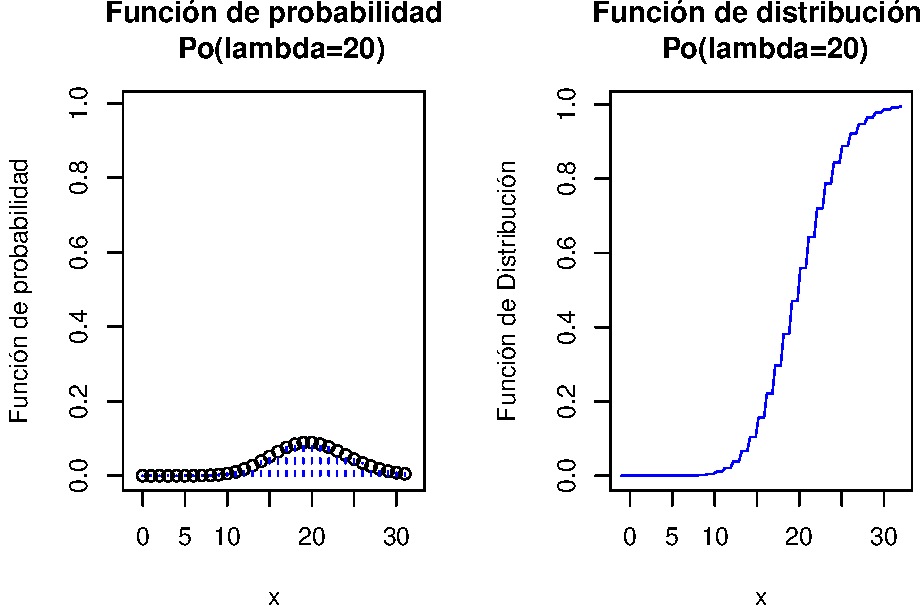
\includegraphics{curso-probabilidad-udemy_files/figure-latex/graficosPOISON-1} \end{center}

\textbf{Gráficos interactivos con \texttt{R}}

Para ejecutar el siguiente gráfico interactivo, solamente tienes que cargar el paquete \texttt{shiny} en tu ordenador y luego copiar/pegar las siguientes instrucciones. De este modo podrás observar los cambios en las distribuciones variando los parámetros.

\begin{Shaded}
\begin{Highlighting}[]
\KeywordTok{sliderInput}\NormalTok{(}\StringTok{"lambda"}\NormalTok{, }\DataTypeTok{label =} \StringTok{"Promedio de eventos lambda"}\NormalTok{,}
              \DataTypeTok{min =} \DecValTok{1}\NormalTok{, }\DataTypeTok{max =} \DecValTok{100}\NormalTok{, }\DataTypeTok{value =}\DecValTok{20}\NormalTok{ , }\DataTypeTok{step =} \DecValTok{1}\NormalTok{)}
\KeywordTok{renderPlot}\NormalTok{(\{}
\NormalTok{  lambda=input}\OperatorTok{$}\NormalTok{lambda}
  \KeywordTok{par}\NormalTok{(}\DataTypeTok{mfrow=}\KeywordTok{c}\NormalTok{(}\DecValTok{1}\NormalTok{,}\DecValTok{2}\NormalTok{))}
\NormalTok{  n=}\KeywordTok{qpois}\NormalTok{(}\FloatTok{0.99}\NormalTok{,}\DataTypeTok{lambda=}\NormalTok{lambda)}
  \CommentTok{#n}
\NormalTok{  aux=}\KeywordTok{rep}\NormalTok{(}\DecValTok{0}\NormalTok{,(n}\OperatorTok{+}\DecValTok{1}\NormalTok{)}\OperatorTok{*}\DecValTok{2}\NormalTok{)}
\NormalTok{  aux[}\KeywordTok{seq}\NormalTok{(}\DecValTok{2}\NormalTok{,(n}\OperatorTok{+}\DecValTok{1}\NormalTok{)}\OperatorTok{*}\DecValTok{2}\NormalTok{,}\DecValTok{2}\NormalTok{)]=}\KeywordTok{dpois}\NormalTok{(}\KeywordTok{c}\NormalTok{(}\DecValTok{0}\OperatorTok{:}\NormalTok{n),}\DataTypeTok{lambda=}\NormalTok{lambda)}
\NormalTok{  ymax=}\FloatTok{0.45}
  \KeywordTok{plot}\NormalTok{(}\DataTypeTok{x=}\KeywordTok{c}\NormalTok{(}\DecValTok{0}\OperatorTok{:}\NormalTok{n),}\DataTypeTok{y=}\KeywordTok{dpois}\NormalTok{(}\KeywordTok{c}\NormalTok{(}\DecValTok{0}\OperatorTok{:}\NormalTok{n),}\DataTypeTok{lambda=}\NormalTok{lambda),}
       \DataTypeTok{ylim=}\KeywordTok{c}\NormalTok{(}\DecValTok{0}\NormalTok{,ymax),}\DataTypeTok{xlim=}\KeywordTok{c}\NormalTok{(}\OperatorTok{-}\DecValTok{1}\NormalTok{,n}\OperatorTok{+}\DecValTok{1}\NormalTok{),}\DataTypeTok{xlab=}\StringTok{"x"}\NormalTok{,}\DataTypeTok{ylab=}\StringTok{"Función de probabilidad"}\NormalTok{,}
       \DataTypeTok{main=}\KeywordTok{paste0}\NormalTok{(}\KeywordTok{c}\NormalTok{(}\StringTok{"Función de probabilidad}\CharTok{\textbackslash{}n}\StringTok{  Po(lambda="}\NormalTok{,lambda,}\StringTok{")"}\NormalTok{),}\DataTypeTok{collapse =} \StringTok{""}\NormalTok{))}
  \KeywordTok{lines}\NormalTok{(}\DataTypeTok{x=}\KeywordTok{rep}\NormalTok{(}\DecValTok{0}\OperatorTok{:}\NormalTok{n,}\DataTypeTok{each=}\DecValTok{2}\NormalTok{),}\DataTypeTok{y=}\NormalTok{aux,}\DataTypeTok{pch=}\DecValTok{21}\NormalTok{, }\DataTypeTok{type =} \StringTok{"h"}\NormalTok{, }\DataTypeTok{lty =} \DecValTok{2}\NormalTok{,}\DataTypeTok{col=}\StringTok{"blue"}\NormalTok{)}
  \KeywordTok{curve}\NormalTok{(}\KeywordTok{ppois}\NormalTok{(x,}\DataTypeTok{lambda=}\NormalTok{lambda),}
        \DataTypeTok{xlim=}\KeywordTok{c}\NormalTok{(}\OperatorTok{-}\DecValTok{1}\NormalTok{,n}\OperatorTok{+}\DecValTok{1}\NormalTok{),}\DataTypeTok{col=}\StringTok{"blue"}\NormalTok{,}\DataTypeTok{ylab=}\StringTok{"Función de Distribución",}
\StringTok{         main=paste0(c("}\NormalTok{Función de distribución \textbackslash{}n }\KeywordTok{Po}\NormalTok{(}\DataTypeTok{lambda=}\StringTok{",lambda,"}\NormalTok{)}\StringTok{"),collapse = ""))}
\StringTok{  par(mfrow=c(1,1))}
\StringTok{\})}
\end{Highlighting}
\end{Shaded}

\textbf{Cálculos con python}

Realicemos los mismos cálculos realizados con \texttt{R} pero ahora usando python. Recordemos que considerábamos una v.a. \(X\) con distribución \(Po(\lambda=3)\). Calculemos \(P_X(0)=P(X=0), P_X(1)=P(X=1)\) con python

\begin{Shaded}
\begin{Highlighting}[]
\ImportTok{from}\NormalTok{ scipy.stats }\ImportTok{import}\NormalTok{ poisson}
\NormalTok{poisson.pmf(}\DecValTok{0}\NormalTok{,mu }\OperatorTok{=} \DecValTok{3}\NormalTok{)}
\end{Highlighting}
\end{Shaded}

\begin{verbatim}
## 0.049787068367863944
\end{verbatim}

\begin{Shaded}
\begin{Highlighting}[]
\NormalTok{poisson.pmf(}\DecValTok{1}\NormalTok{,mu }\OperatorTok{=} \DecValTok{3}\NormalTok{)}
\end{Highlighting}
\end{Shaded}

\begin{verbatim}
## 0.14936120510359185
\end{verbatim}

Si quisiéramos hallar las funciones de distribución en los mismos valores anteriores,
\(F_X(0)=P(X\leq 0), F_X(1)=P(X\leq 1)\), tendríamos que hacer:

\begin{Shaded}
\begin{Highlighting}[]
\NormalTok{poisson.cdf(}\DecValTok{0}\NormalTok{,mu }\OperatorTok{=} \DecValTok{3}\NormalTok{)}
\end{Highlighting}
\end{Shaded}

\begin{verbatim}
## 0.049787068367863951
\end{verbatim}

\begin{Shaded}
\begin{Highlighting}[]
\NormalTok{poisson.cdf(}\DecValTok{1}\NormalTok{,mu }\OperatorTok{=} \DecValTok{3}\NormalTok{)}
\end{Highlighting}
\end{Shaded}

\begin{verbatim}
## 0.19914827347145581
\end{verbatim}

\begin{Shaded}
\begin{Highlighting}[]
\NormalTok{poisson.pmf(}\DecValTok{0}\NormalTok{,mu }\OperatorTok{=} \DecValTok{3}\NormalTok{)}\OperatorTok{+}\NormalTok{poisson.pmf(}\DecValTok{1}\NormalTok{,mu}\OperatorTok{=} \DecValTok{3}\NormalTok{) }\CommentTok{### es igual a poisson.cdf(1,lambda=3)}
\end{Highlighting}
\end{Shaded}

\begin{verbatim}
## 0.19914827347145581
\end{verbatim}

La comprobación de que \(F_X(10)=\displaystyle\sum_{0}^{10} P_X(x)\) en python se realiza de la forma siguiente:

\begin{Shaded}
\begin{Highlighting}[]
\BuiltInTok{range}\NormalTok{(}\DecValTok{0}\NormalTok{,}\DecValTok{10}\NormalTok{)}
\end{Highlighting}
\end{Shaded}

\begin{verbatim}
## [0, 1, 2, 3, 4, 5, 6, 7, 8, 9]
\end{verbatim}

\begin{Shaded}
\begin{Highlighting}[]
\NormalTok{poisson.pmf(}\BuiltInTok{range}\NormalTok{(}\DecValTok{0}\NormalTok{,}\DecValTok{10}\NormalTok{),mu}\OperatorTok{=}\DecValTok{3}\NormalTok{)}
\end{Highlighting}
\end{Shaded}

\begin{verbatim}
## array([ 0.04978707,  0.14936121,  0.22404181,  0.22404181,  0.16803136,
##         0.10081881,  0.05040941,  0.02160403,  0.00810151,  0.0027005 ])
\end{verbatim}

\begin{Shaded}
\begin{Highlighting}[]
\BuiltInTok{sum}\NormalTok{(poisson.pmf(}\BuiltInTok{range}\NormalTok{(}\DecValTok{0}\NormalTok{,}\DecValTok{10}\NormalTok{),mu}\OperatorTok{=}\DecValTok{3}\NormalTok{))}
\end{Highlighting}
\end{Shaded}

\begin{verbatim}
## 0.99889751186988462
\end{verbatim}

\begin{Shaded}
\begin{Highlighting}[]
\NormalTok{poisson.cdf(}\DecValTok{10}\NormalTok{,mu}\OperatorTok{=}\DecValTok{3}\NormalTok{)}
\end{Highlighting}
\end{Shaded}

\begin{verbatim}
## 0.99970766304935266
\end{verbatim}

\textbf{Ejercicio de la trampa para insectos (continuación)}

En el ejercicio de la trampa para insectos teníamos que \(X\) es una \(Po(20)\). Responded con python a la preguntas 3 y 4 de este ejercicio

\textbf{Pregunta 3.} Calculad la probabilidad de que en una hora caigan en la trampa exactamente 21 insectos.

Recordemos que la probabilidad pedida es \(P(X=21)\):

\begin{Shaded}
\begin{Highlighting}[]
\NormalTok{poisson.pmf(}\DecValTok{21}\NormalTok{,mu}\OperatorTok{=}\DecValTok{20}\NormalTok{)}
\CommentTok{## P(X=21)}
\end{Highlighting}
\end{Shaded}

\begin{verbatim}
## 0.084605064182937909
\end{verbatim}

\textbf{Pregunta 4.} Calculad la probabilidad de que en una hora caigan en la trampa al menos 6 insectos.

La probabilidad pedida es \(P(X\geq 6)=1-P(X\leq 5)\):

\begin{Shaded}
\begin{Highlighting}[]
\DecValTok{1}\OperatorTok{-}\NormalTok{poisson.cdf(}\DecValTok{5}\NormalTok{,mu}\OperatorTok{=}\DecValTok{20}\NormalTok{) }
\CommentTok{## es 1-P(X<=5)=P(X>=6)}
\end{Highlighting}
\end{Shaded}

\begin{verbatim}
## 0.99992809115947157
\end{verbatim}

Como ya hemos visto con \texttt{scipy.stats}, podemos pedir los momentos de una variable aleatoria
\(Po(3)\)

\begin{Shaded}
\begin{Highlighting}[]
\NormalTok{poisson.stats(mu}\OperatorTok{=}\DecValTok{3}\NormalTok{, moments}\OperatorTok{=}\StringTok{'mv'}\NormalTok{)}
\end{Highlighting}
\end{Shaded}

\begin{verbatim}
## (array(3.0), array(3.0))
\end{verbatim}

Y también generar secuencias de observaciones aleatorias de una población \(Po(3)\):

\begin{Shaded}
\begin{Highlighting}[]
\NormalTok{poisson.rvs(mu}\OperatorTok{=}\DecValTok{3}\NormalTok{,size}\OperatorTok{=}\DecValTok{40}\NormalTok{)}
\end{Highlighting}
\end{Shaded}

\begin{verbatim}
## array([2, 3, 2, 1, 3, 3, 3, 1, 6, 5, 2, 3, 2, 5, 4, 2, 2, 3, 3, 0, 4, 4, 5,
##        3, 6, 3, 2, 1, 1, 4, 3, 3, 4, 6, 2, 0, 4, 4, 3, 2])
\end{verbatim}

\textbf{Gráficos con python}

\begin{Shaded}
\begin{Highlighting}[]
\ImportTok{from}\NormalTok{ scipy.stats }\ImportTok{import}\NormalTok{ poisson}
\NormalTok{mu }\OperatorTok{=} \DecValTok{10} \CommentTok{## mu = lambda}
\NormalTok{x }\OperatorTok{=}\NormalTok{ np.arange(poisson.ppf(}\FloatTok{0.01}\NormalTok{, mu),poisson.ppf(}\FloatTok{0.99}\NormalTok{, mu))}
\NormalTok{fig }\OperatorTok{=}\NormalTok{plt.figure(figsize}\OperatorTok{=}\NormalTok{(}\DecValTok{5}\NormalTok{, }\FloatTok{2.7}\NormalTok{))}
\NormalTok{ax }\OperatorTok{=}\NormalTok{ fig.add_subplot(}\DecValTok{1}\NormalTok{,}\DecValTok{2}\NormalTok{,}\DecValTok{1}\NormalTok{)}
\NormalTok{ax.plot(x, poisson.pmf(x, mu), }\StringTok{'bo'}\NormalTok{, ms}\OperatorTok{=}\DecValTok{5}\NormalTok{, label}\OperatorTok{=}\StringTok{'Poisson pmf'}\NormalTok{)}
\NormalTok{ax.vlines(x, }\DecValTok{0}\NormalTok{, poisson.pmf(x, mu), colors}\OperatorTok{=}\StringTok{'b'}\NormalTok{, lw}\OperatorTok{=}\DecValTok{2}\NormalTok{, alpha}\OperatorTok{=}\FloatTok{0.5}\NormalTok{)}
\ControlFlowTok{for}\NormalTok{ tick }\KeywordTok{in}\NormalTok{ ax.xaxis.get_major_ticks():}
\NormalTok{  tick.label.set_fontsize(}\DecValTok{5}\NormalTok{)}
\ControlFlowTok{for}\NormalTok{ tick }\KeywordTok{in}\NormalTok{ ax.yaxis.get_major_ticks():}
\NormalTok{  tick.label.set_fontsize(}\DecValTok{5}\NormalTok{) }
\NormalTok{ax }\OperatorTok{=}\NormalTok{ fig.add_subplot(}\DecValTok{1}\NormalTok{,}\DecValTok{2}\NormalTok{,}\DecValTok{2}\NormalTok{)}
\NormalTok{ax.plot(x, poisson.cdf(x, mu), }\StringTok{'bo'}\NormalTok{, ms}\OperatorTok{=}\DecValTok{5}\NormalTok{, label}\OperatorTok{=}\StringTok{'Poisson cdf'}\NormalTok{)}
\NormalTok{ax.vlines(x, }\DecValTok{0}\NormalTok{, poisson.cdf(x, mu), colors}\OperatorTok{=}\StringTok{'b'}\NormalTok{, lw}\OperatorTok{=}\DecValTok{2}\NormalTok{, alpha}\OperatorTok{=}\FloatTok{0.5}\NormalTok{)}
\ControlFlowTok{for}\NormalTok{ tick }\KeywordTok{in}\NormalTok{ ax.xaxis.get_major_ticks():}
\NormalTok{  tick.label.set_fontsize(}\DecValTok{5}\NormalTok{)}
\ControlFlowTok{for}\NormalTok{ tick }\KeywordTok{in}\NormalTok{ ax.yaxis.get_major_ticks():}
\NormalTok{  tick.label.set_fontsize(}\DecValTok{5}\NormalTok{)}
\NormalTok{fig.suptitle(}\StringTok{'Distribucion de Poisson'}\NormalTok{)}
\NormalTok{plt.show()}
\end{Highlighting}
\end{Shaded}

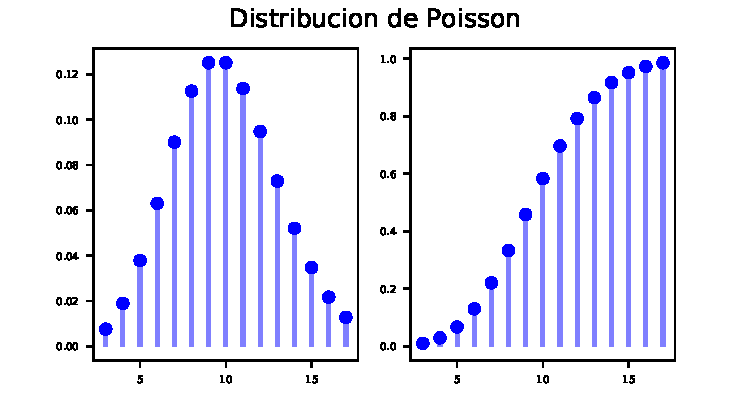
\includegraphics{curso-probabilidad-udemy_files/figure-latex/py_poiss2-1.pdf}

\textbf{Gráficos interactivos para un proceso de Poisson \(Po(\lambda\cdot t\))}

Para ejecutar el siguiente gráfico interactivo, solamente tienes que cargar el paquete \texttt{shiny} en tu ordenador y luego copiar/pegar las siguientes instrucciones. De este modo podrás observar los cambios en las distribuciones variando los parámetros.

\begin{Shaded}
\begin{Highlighting}[]
\KeywordTok{fluidPage}\NormalTok{(}
  \KeywordTok{fluidRow}\NormalTok{(}
      \KeywordTok{column}\NormalTok{(}\DecValTok{6}\NormalTok{,}
           \KeywordTok{sliderInput}\NormalTok{(}\StringTok{"lambdapp"}\NormalTok{, }\DataTypeTok{label=}\StringTok{"Promedio eventos por unidad de tiempo"}\NormalTok{, }
                       \DataTypeTok{min =} \FloatTok{0.1}\NormalTok{, }\DataTypeTok{max =} \DecValTok{50}\NormalTok{, }\DataTypeTok{value =}\DecValTok{10}\NormalTok{ , }\DataTypeTok{step =} \FloatTok{0.01}\NormalTok{)),}
    \KeywordTok{column}\NormalTok{(}\DecValTok{6}\NormalTok{,}\KeywordTok{sliderInput}\NormalTok{(}\StringTok{"t"}\NormalTok{, }\DataTypeTok{label =} \StringTok{"Intervalo de tiempo (0,t]"}\NormalTok{, }
                         \DataTypeTok{min =} \DecValTok{1}\NormalTok{, }\DataTypeTok{max =} \DecValTok{120}\NormalTok{, }\DataTypeTok{value =}\DecValTok{1}\NormalTok{ , }\DataTypeTok{step =} \FloatTok{0.5}\NormalTok{))}
\NormalTok{   )}
\NormalTok{)}


\KeywordTok{renderPlot}\NormalTok{(\{}
\NormalTok{  lambda1=input}\OperatorTok{$}\NormalTok{lambdapp}
\NormalTok{  t=input}\OperatorTok{$}\NormalTok{t}
\NormalTok{  lambda=lambda1}\OperatorTok{*}\NormalTok{t }\CommentTok{## es lambda* t}
  \KeywordTok{par}\NormalTok{(}\DataTypeTok{mfrow=}\KeywordTok{c}\NormalTok{(}\DecValTok{1}\NormalTok{,}\DecValTok{2}\NormalTok{))}
\NormalTok{  n=}\KeywordTok{qpois}\NormalTok{(}\FloatTok{0.99}\NormalTok{,}\DataTypeTok{lambda=}\NormalTok{lambda)}
  \CommentTok{#n}
\NormalTok{  aux=}\KeywordTok{rep}\NormalTok{(}\DecValTok{0}\NormalTok{,(n}\OperatorTok{+}\DecValTok{1}\NormalTok{)}\OperatorTok{*}\DecValTok{2}\NormalTok{)}
\NormalTok{  aux[}\KeywordTok{seq}\NormalTok{(}\DecValTok{2}\NormalTok{,(n}\OperatorTok{+}\DecValTok{1}\NormalTok{)}\OperatorTok{*}\DecValTok{2}\NormalTok{,}\DecValTok{2}\NormalTok{)]=}\KeywordTok{dpois}\NormalTok{(}\KeywordTok{c}\NormalTok{(}\DecValTok{0}\OperatorTok{:}\NormalTok{n),}\DataTypeTok{lambda=}\NormalTok{lambda)}
\NormalTok{  ymax=}\KeywordTok{ppois}\NormalTok{(}\KeywordTok{which.max}\NormalTok{(}\KeywordTok{ppois}\NormalTok{(}\DecValTok{0}\OperatorTok{:}\NormalTok{n,lambda))}\OperatorTok{-}\DecValTok{1}\NormalTok{,lambda)}\OperatorTok{*}\FloatTok{0.7}
  \KeywordTok{plot}\NormalTok{(}\DataTypeTok{x=}\KeywordTok{c}\NormalTok{(}\DecValTok{0}\OperatorTok{:}\NormalTok{n),}\DataTypeTok{y=}\KeywordTok{dpois}\NormalTok{(}\KeywordTok{c}\NormalTok{(}\DecValTok{0}\OperatorTok{:}\NormalTok{n),}\DataTypeTok{lambda=}\NormalTok{lambda),}
       \DataTypeTok{ylim=}\KeywordTok{c}\NormalTok{(}\DecValTok{0}\NormalTok{,ymax),}\DataTypeTok{xlim=}\KeywordTok{c}\NormalTok{(}\OperatorTok{-}\DecValTok{1}\NormalTok{,n}\OperatorTok{+}\DecValTok{1}\NormalTok{),}\DataTypeTok{xlab=}\StringTok{"x"}\NormalTok{,}\DataTypeTok{ylab=}\StringTok{"Función de probabilidad"}\NormalTok{,}
       \DataTypeTok{main=}\KeywordTok{paste0}\NormalTok{(}\KeywordTok{c}\NormalTok{(}\StringTok{"Función de probabilidad}\CharTok{\textbackslash{}n}\StringTok{  Po(lambda="}\NormalTok{,lambda,}\StringTok{")"}\NormalTok{),}\DataTypeTok{collapse =} \StringTok{""}\NormalTok{))}
  \KeywordTok{lines}\NormalTok{(}\DataTypeTok{x=}\KeywordTok{rep}\NormalTok{(}\DecValTok{0}\OperatorTok{:}\NormalTok{n,}\DataTypeTok{each=}\DecValTok{2}\NormalTok{),}\DataTypeTok{y=}\NormalTok{aux,}\DataTypeTok{pch=}\DecValTok{21}\NormalTok{, }\DataTypeTok{type =} \StringTok{"h"}\NormalTok{, }\DataTypeTok{lty =} \DecValTok{2}\NormalTok{,}\DataTypeTok{col=}\StringTok{"blue"}\NormalTok{)}
  \KeywordTok{curve}\NormalTok{(}\KeywordTok{ppois}\NormalTok{(x,}\DataTypeTok{lambda=}\NormalTok{lambda),}
        \DataTypeTok{xlim=}\KeywordTok{c}\NormalTok{(}\OperatorTok{-}\DecValTok{1}\NormalTok{,n}\OperatorTok{+}\DecValTok{1}\NormalTok{),}\DataTypeTok{col=}\StringTok{"blue"}\NormalTok{,}\DataTypeTok{ylab=}\StringTok{"Función de Distribución",}
\StringTok{         main=paste0(c("}\NormalTok{Función de distribución \textbackslash{}n }\KeywordTok{Po}\NormalTok{(}\DataTypeTok{lambda=}\StringTok{",lambda,"}\NormalTok{)}\StringTok{"),collapse = ""))}
\StringTok{  par(mfrow=c(1,1))}
\StringTok{  \})}
\end{Highlighting}
\end{Shaded}

\textbf{Ejemplo: Número de impactos de insectos en la visera de un casco}

Un colega de trabajo, al que llamaremos JG, es muy aficionado a los grandes premios de velocidad tanto en coches como en motos.

Como es tan aficionado, está obsesionado con muchas de las más extravagantes estadísticas de estos deportes.
En particular le propusimos que estudiara el número de insectos que chocan contra la visera de un casco de un motorista GP o de un conductor de fórmula 1 .

La idea es que el número de insectos está igualmente repartido por todo el circuito y de promedio impactan \(\lambda>0\) insectos por minuto. También es razonable suponer que:

\begin{itemize}
\tightlist
\item
  podemos dividir la superficie de la visera en cuadrados suficientemente pequeños de forma que la probabilidad de que caigan dos insectos en la misma zona es prácticamente 0.
\item
  la probabilidad de que un insecto impacte en un cuadrado cualquiera de la visera es independiente de cualquier otro cuadrado.
\item
  si hemos dividido la visera en \(n\) cuadrados la probabilidad \(p_n\) de impacto de un cuadrado vale \(p_n=\frac{\lambda}{n}\).
\end{itemize}

Bajo estas condiciones, si denotamos por \(X_t\) como el número de insectos que ha impactado en la visera en el intervalo \((0,t]\) (en \(t\) minutos), podemos afirmar que \(X_t\) es un proceso de Poisson \(Po(\lambda\cdot t)\).

Supongamos que nos dicen que \(\lambda=3\) insectos por minuto. Entonces el proceso de Poisson \(X_t\) seguirá un ley \(Po(3\cdot t).\)

Nos piden las probabilidades siguientes:

\begin{enumerate}
\def\labelenumi{\arabic{enumi}.}
\tightlist
\item
  ¿Cuál es la probabilidad de que en 10 minutos impacten más de 25 insectos?
\item
  ¿Cuál es la probabilidad de que tengamos que esperar más de 2 minutos para observar el primer impacto?
\end{enumerate}

\textbf{Solución de 1. ¿Cuál es la probabilidad de que en 10 minutos impacten más de 25 insectos?}

En este caso \(t=10\) y \(X_{10}\) es la variable aleatoria que nos da el número de insectos que impactan en 10 minutos o durante el intervalo \([0,10)\). La distribución de \(X_{10}\) será de Poisson de parámetro \(\lambda=3\cdot 10=30)\), \(Po(30)\).

Nos piden la probabilidad siguiente: \(P(X>25)=1-P(X\leq 25)\), que calculamos con ayuda de \texttt{R}:

\begin{Shaded}
\begin{Highlighting}[]
\DecValTok{1}\OperatorTok{-}\KeywordTok{dpois}\NormalTok{(}\DecValTok{25}\NormalTok{,}\DataTypeTok{lambda=}\DecValTok{3}\NormalTok{)}
\end{Highlighting}
\end{Shaded}

\begin{verbatim}
## [1] 1
\end{verbatim}

\textbf{Solución de 2. ¿Cuál es la probabilidad de que tengamos que esperar más de 2 minutos para observar el primer impacto?}

Nos piden la probabilidad siguiente \(P(X_2=0)\) ya que la variable \(X_2\) nos dice el número de impactos en dos minutos. La distribución de \(X_2\) será de Poisson de parámetro \(\lambda =2\cdot 3=6\), \(Po(6)\). Si hemos de esperar más de dos minutos para el primer impacto, significa que \(X_2=0\):
\[P(X_2=0)=\frac{(6)^0}{0!}\cdot e^{-6}= e^{-6}=0.002479.\]
Si usamos \texttt{R}, obtenemos:

\begin{Shaded}
\begin{Highlighting}[]
\DecValTok{6}\OperatorTok{^}\DecValTok{0}\OperatorTok{/}\KeywordTok{factorial}\NormalTok{(}\DecValTok{0}\NormalTok{)}\OperatorTok{*}\KeywordTok{exp}\NormalTok{(}\OperatorTok{-}\DecValTok{6}\NormalTok{)}
\end{Highlighting}
\end{Shaded}

\begin{verbatim}
## [1] 0.002478752
\end{verbatim}

\begin{Shaded}
\begin{Highlighting}[]
\KeywordTok{ppois}\NormalTok{(}\DecValTok{0}\NormalTok{,}\DataTypeTok{lambda=}\DecValTok{3}\OperatorTok{*}\DecValTok{2}\NormalTok{)}
\end{Highlighting}
\end{Shaded}

\begin{verbatim}
## [1] 0.002478752
\end{verbatim}

\hypertarget{distribuciuxf3n-hipergeomuxe9trica}{%
\subsection{Distribución hipergeométrica}\label{distribuciuxf3n-hipergeomuxe9trica}}

Supongamos que disponemos de una urna de de sorteos que contiene \(m\) bolas blancas y \(n\) bolas rojas.

En total en esta urna hay \(m+n\) bolas, \(m\) blancas y \(n\) rojas. Si extraemos dos bolas de la urna lo podemos hacer de dos formas:

\begin{itemize}
\tightlist
\item
  Extraer una anotar su color y reponerla. Sacar otra y anotar su color. Hemos extraído la bola con reposición.
\item
  Extraer simultáneamente dos bolas (sin reposición) y contar el número de bolas blancas.
\end{itemize}

Sea \(X\) la v.a. que cuenta el número de bolas blancas extraídas.

Sea \(X\) es la v.a. que cuenta el número de bolas blancas extraídas.

\begin{itemize}
\tightlist
\item
  En el primer caso, \(X\) es una \(B(n=2,p=\frac{m}{m+n})\) ya que consiste en repetir dos veces el mismo experimento de Bernoulli.
\item
  En el segundo caso, \(X\) sigue una distribución hipergeométrica que estudiaremos en esta sección.
\end{itemize}

 \textbf{Distribución hipergeométrica}

Sean \(n\), \(m\) y \(k\) tres número enteros positivos y tales que \(k<m+n\).

Consideremos una urna que contiene \(m+n\) bolas de las que \(m\) son blancas y las restantes \(n\) no (son no blancas).

El número total de bolas es \(m+n\). Extraemos de forma aleatoria \(k\) bolas de la urna sin reemplazarlas.

Sea \(X\) la v.a. que cuenta el número de bolas blancas extraídas. Diremos que la distribución de \(X\) es hipergeométrica de parámetros \(m\), \(n\) y \(k\) y la denotaremos por \(H(m,n,k)\).

Su dominio es

\[D_X=\left\{x\in\mathbf{N}\mid \max\{0,k-n\}\leq  x \leq \min\{m,k\}\right\}\]

Para explicarlo, veamos varios ejemplos:

\begin{itemize}
\tightlist
\item
  \(H(m=5,n=2,k=3)\). Tenemos \(m=5\) bolas blancas, \(n=2\) no blancas y sacamos \(k=3\) bolas sin reposición.

  \begin{itemize}
  \tightlist
  \item
    En este caso el mínimo de bolas blancas extraídas es \(1=k-n=3-2\), ya que sólo hay dos no blancas.
  \item
    En cambio, el máximo si es \(k=3\), ya que tenemos bolas blancas de ``sobra''.
  \end{itemize}
\item
  \(H(m=2,n=5,k=3)\). Tenemos \(m=2\) bolas blancas, \(n=5\) no blancas y sacamos \(k=3\) bolas sin reposición.

  \begin{itemize}
  \tightlist
  \item
    En este caso el mínimo de bolas blancas es \(0\) ya que puedo sacar 3 no blancas.
  \item
    En cambio, el máximo si es \(m=2\), ya que aunque saquemos \(k=3\) bolas, al llegar a 2 ya hemos extraído todas las bolas blancas de la urna.
  \end{itemize}
\item
  \(H(m=10,n=10,k=3)\). Tenemos \(m=10\) bolas blancas, \(n=10\) no blancas y sacamos \(k=3\) bolas sin reposición.

  \begin{itemize}
  \tightlist
  \item
    En este caso podemos obtener desde \(0\) blancas hasta \(k=3\) blancas.
  \end{itemize}
\end{itemize}

Su función de probabilidad es:
\[
P_{X}(x)=\left\{
\begin{array}{ll}
\frac{\binom{m}{x}\cdot \binom{n}{k-x}}{\binom{m+n}{k}}, & \mbox{ si }
\max\{0,k-n\}\leq x \leq \min\{m,k\}, \mbox { para  } x\in \mathbf{N},\\
0,  & \mbox{en otro caso.}\end{array}\right.
\]

 \textbf{Observación: otras parametrizaciones}

En ocasiones se parametriza una v.a. hipergeométrica mediante \(N=m+n\), número total de bolas,
\(k\), número de extracciones y \(p\), probabilidad de extraer una bola blanca.

Así, podemos \textbf{parametrizar alternativamente} la distribución hipergeométrica como
\(H(N,k,p)\) donde \(p=\frac{m}{N}.\)

\textbf{Resumen hipergeométrica \(H(m,n,k)\)}

\begin{longtable}[]{@{}rl@{}}
\toprule
\begin{minipage}[b]{0.47\columnwidth}\raggedleft
\(X=\)número de bolas blancas en \(k\) extracciones sin reposición de una urna con \(m\) bolas blancas y \(n\) negras.\strut
\end{minipage} & \begin{minipage}[b]{0.47\columnwidth}\raggedright
\(H(m,n,k)\)\strut
\end{minipage}\tabularnewline
\midrule
\endhead
\begin{minipage}[t]{0.47\columnwidth}\raggedleft
\(D_X\)=\strut
\end{minipage} & \begin{minipage}[t]{0.47\columnwidth}\raggedright
\(\left\{x\in\mathbf{N}\mid \max\{0,k-n\}\leq x \leq \min\{m,k\}\right\}\)\strut
\end{minipage}\tabularnewline
\begin{minipage}[t]{0.47\columnwidth}\raggedleft
\(P_X(x)=P(X=x)=\)\strut
\end{minipage} & \begin{minipage}[t]{0.47\columnwidth}\raggedright
\(\left\{ \begin{array}{ll} \frac{\binom{m}{x}\cdot \binom{n}{k-x}}{\binom{m+n}{k}}, & \mbox{ si } \max\{0,k-n\}\leq x \leq \min\{m,k\}, \\ 0, & \mbox{en otro caso.}\end{array}\right.\)\strut
\end{minipage}\tabularnewline
\begin{minipage}[t]{0.47\columnwidth}\raggedleft
\(F_X(x)=P(X\leq x)\)\strut
\end{minipage} & \begin{minipage}[t]{0.47\columnwidth}\raggedright
Hay que sumarla. Utilizad funciones de \texttt{R} o de python.\strut
\end{minipage}\tabularnewline
\begin{minipage}[t]{0.47\columnwidth}\raggedleft
\(E(X)=\frac{k\cdot m}{m+n}\)\strut
\end{minipage} & \begin{minipage}[t]{0.47\columnwidth}\raggedright
\(Var(X)=k\cdot\frac{m}{m+n}\cdot\left(1-\frac{m}{m+n}\right) \cdot\frac{m+n-k}{m+n-1}\)\strut
\end{minipage}\tabularnewline
\bottomrule
\end{longtable}

\textbf{Ejemplo: urna con \(m=15\) blancas, \(n=10\) rojas y \(k=3\) extracciones sin reposición}

Tenemos una urna con 15 bolas blancas y 10 bolas rojas. Extraemos al azar tres bolas de la urna sin reposición. Sea \(X\) el número de bolas \textbf{blancas} extraídas. Bajo esta condiciones, la v.a. \(X\) sigue una ley de distribución \(H(m=15,n=10,k=3)\).

Nos piden:

\begin{enumerate}
\def\labelenumi{\arabic{enumi}.}
\tightlist
\item
  Hallar la función de probabilidad de \(X\).
\item
  Probabilidad de sacar dos bolas blancas.
\item
  Probabilidad de sacar más de una bola blanca.
\item
  Esperanza, varianza y desviación típica de \(X\).
\end{enumerate}

\textbf{Solución de 1. Hallar la función de probabilidad de \(X\)}

La función de probabilidad de \(X\) es:
\[
P_X(x)=P(X=x)=\left\{
\begin{array}{ll}
\frac{\binom{m}{x}\cdot \binom{n}{k-x}}{\binom{m+n}{k}}, & \mbox{ si }
\max\{0,k-n\}\leq x \leq \min\{m,k\}, \mbox { para  } x\in \mathbf{N},\\
0,  & \mbox{en otro caso.}\end{array}\right.
\]

Sustituyendo los parámetros \(m,n\) y \(k\) por \(m=15\), \(n=10\) y \(k=3\), obtenemos:

\[
P_X(x)=P(X=x)=\left\{
\begin{array}{ll}
\frac{\binom{15}{x}\cdot \binom{10}{3-x}}{\binom{25}{3}}= \frac{\binom{15}{x}\cdot \binom{10}{3-x}}{2300}, & \mbox{ si }
0\leq x \leq 3, \mbox { para  } x\in \mathbf{N},\\
0,  & \mbox{en otro caso.}\end{array}\right.
\]

\textbf{Solución de 2. Probabilidad de sacar dos bolas blancas}

La probabilidad de sacar 2 blancas será:
\[
P(X=2)=\frac{\binom{15}{2}\cdot \binom{10}{3-2}}{\binom{25}{3}}
\]

Si calculamos con ayuda de \texttt{R} los números binomiales involucrados en la expresión anterior, obtenemos:

\begin{Shaded}
\begin{Highlighting}[]
\KeywordTok{c}\NormalTok{(}\KeywordTok{choose}\NormalTok{(}\DecValTok{15}\NormalTok{,}\DecValTok{2}\NormalTok{), }\KeywordTok{choose}\NormalTok{(}\DecValTok{10}\NormalTok{,}\DecValTok{1}\NormalTok{), }\KeywordTok{choose}\NormalTok{(}\DecValTok{25}\NormalTok{,}\DecValTok{3}\NormalTok{))}
\end{Highlighting}
\end{Shaded}

\begin{verbatim}
## [1]  105   10 2300
\end{verbatim}

La probabilidad pedida, será, pues:
\(P(X=2)=\frac{105\cdot10 }{2300}=0.4565217.\)

\textbf{Solución de 3. Probabilidad de sacar más de una bola blanca}

La probabilidad de que saquemos más de 1 bola blanca es:
\[
\begin{array}{rl}
P(X> 1)&= 1-P(X\leq 1)=1-(P(X=0)+P(X=1))\\
&=
1-\left(\frac{\binom{15}{0}\cdot \binom{10}{3}}{\binom{25}{3}}+
\frac{\binom{15}{1}\cdot \binom{10}{2}}{\binom{25}{3}}\right)\\
&=
1-\left(
\frac{1\cdot120 }{2300}+\frac{15\cdot45 }{2300}
\right)=1-\frac{120+15\cdot 45}{2300}=0.6543478.
\end{array}
\]

\textbf{Solución de 4. Esperanza, varianza y desviación típica de \(X\)}

El número esperado de bolas blancas extraídas para una v.a. \(X\) de distribución \(H(m=15,n=10,k=3)\) es:

\[E(X)=\frac{k\cdot m}{m+n}=\frac{3\cdot 15}{15+10}=\frac{45}{35}=1.285714.\]
La varianza vale:
\[
\begin{array}{rl}
Var(X)&=k\cdot\frac{m}{m+n}\cdot\left(1-\frac{m}{m+n}\right) \cdot\frac{m+n-k}{m+n-1}\\
&=3\cdot\frac{15}{15+10}\cdot\left(1-\frac{15}{15+10}\right) \cdot\frac{15+10-3}{15+10-1}\\
&=
3\cdot\frac{15}{25}\cdot\left(1-\frac{15}{25}\right) \cdot\frac{22}{24}= 
3\cdot\frac{15}{25}\cdot\frac{25-15}{25} \cdot\frac{22}{24}\\
&=
3\cdot\frac{15}{25}\cdot\frac{10}{25}\cdot\frac{22}{24}=0.66.
\end{array}
\]

Y por lo tanto, su desviación típica es:

\[
+\sqrt{Var(X)}=+\sqrt{0.66}=0.812404.
\]

\textbf{Cálculos con R}

Sea \(X\) una v.a. \(H(m,n,k)\). La función de \texttt{R} para calcular la función de probabilidad en un valor \(x\), \(P(X=x)\), es \texttt{dhyper(x,m,n,k)} y para calcular la función de distribución en un valor \(q\), \(P(X\leq q)\), es \texttt{phyper(q,m,n,k)}. Para generar una muestra de valores que siga la distribución \(H(m,n,k)\), hay que usar la función \texttt{rhyper(nn,m,n,k)} donde \texttt{nn} es el número de observaciones aleatorias deseado de la muestra.

Por ejemplo, si \(X\) es una \(H(m=15,n=10,k=3)\), los valores de \(P(X=2)\) y que \(P(X>1)=1-P(X\leq 1)\) son:

\begin{Shaded}
\begin{Highlighting}[]
\KeywordTok{dhyper}\NormalTok{(}\DataTypeTok{x=}\DecValTok{2}\NormalTok{,}\DataTypeTok{m=}\DecValTok{15}\NormalTok{,}\DecValTok{10}\NormalTok{,}\DataTypeTok{k=}\DecValTok{3}\NormalTok{)}
\end{Highlighting}
\end{Shaded}

\begin{verbatim}
## [1] 0.4565217
\end{verbatim}

\begin{Shaded}
\begin{Highlighting}[]
\KeywordTok{phyper}\NormalTok{(}\DataTypeTok{q=}\DecValTok{1}\NormalTok{,}\DataTypeTok{m=}\DecValTok{15}\NormalTok{,}\DataTypeTok{n=}\DecValTok{10}\NormalTok{,}\DataTypeTok{k=}\DecValTok{3}\NormalTok{)}\CommentTok{## sí, le han puesto q ya veremos el porqué}
\end{Highlighting}
\end{Shaded}

\begin{verbatim}
## [1] 0.3456522
\end{verbatim}

\begin{Shaded}
\begin{Highlighting}[]
\DecValTok{1}\OperatorTok{-}\KeywordTok{phyper}\NormalTok{(}\DataTypeTok{q=}\DecValTok{1}\NormalTok{,}\DataTypeTok{m=}\DecValTok{15}\NormalTok{,}\DataTypeTok{n=}\DecValTok{10}\NormalTok{,}\DataTypeTok{k=}\DecValTok{3}\NormalTok{)}
\end{Highlighting}
\end{Shaded}

\begin{verbatim}
## [1] 0.6543478
\end{verbatim}

Una muestra aleatoria de este experimento de tamaño 200 sería:

\begin{Shaded}
\begin{Highlighting}[]
\KeywordTok{rhyper}\NormalTok{(}\DataTypeTok{nn=}\DecValTok{200}\NormalTok{,}\DataTypeTok{m=}\DecValTok{15}\NormalTok{,}\DataTypeTok{n=}\DecValTok{10}\NormalTok{,}\DataTypeTok{k=}\DecValTok{3}\NormalTok{)}
\end{Highlighting}
\end{Shaded}

\begin{verbatim}
##   [1] 2 3 1 3 1 2 2 3 2 2 1 2 1 2 2 3 3 1 1 1 1 0 2 3 2 1 3 2 2 2 2 3 2 3 3 2 0
##  [38] 1 2 1 3 2 2 3 2 3 2 2 3 2 3 1 2 2 2 2 3 2 2 1 3 2 2 3 1 2 2 2 2 2 3 0 2 0
##  [75] 3 2 2 2 1 2 2 3 1 1 1 2 2 2 2 1 1 3 2 2 3 2 2 1 1 1 3 3 2 2 2 1 3 2 2 2 1
## [112] 1 2 3 2 2 1 2 2 2 2 2 2 3 1 2 3 3 1 1 2 2 1 1 3 2 1 1 2 2 3 1 1 1 2 1 1 3
## [149] 1 2 2 3 3 2 3 1 2 1 2 2 2 1 2 3 1 3 3 3 2 2 1 3 3 1 1 2 2 2 2 2 3 2 1 2 1
## [186] 1 1 1 2 1 1 2 2 2 2 3 3 1 0 2
\end{verbatim}

\textbf{Gráficas con R}

Los gráficos de la función de probabilidad y de la función de distribución en \texttt{R} se realizan de la forma siguiente:

\begin{Shaded}
\begin{Highlighting}[]
\KeywordTok{par}\NormalTok{(}\DataTypeTok{mfrow=}\KeywordTok{c}\NormalTok{(}\DecValTok{1}\NormalTok{,}\DecValTok{2}\NormalTok{))}
\NormalTok{m=}\DecValTok{15}
\NormalTok{n=}\DecValTok{10}
\NormalTok{k=}\DecValTok{3}
\NormalTok{a=}\KeywordTok{max}\NormalTok{(}\KeywordTok{c}\NormalTok{(}\DecValTok{0}\NormalTok{,k}\OperatorTok{-}\NormalTok{n))}
\NormalTok{b=}\KeywordTok{min}\NormalTok{(}\KeywordTok{c}\NormalTok{(m,k))}
\NormalTok{l=b}\OperatorTok{-}\NormalTok{a}\OperatorTok{+}\DecValTok{1}
\NormalTok{aux=}\KeywordTok{rep}\NormalTok{(}\DecValTok{0}\NormalTok{,}\DecValTok{2}\OperatorTok{*}\NormalTok{l)}
\NormalTok{aux[}\KeywordTok{seq}\NormalTok{(}\DecValTok{2}\NormalTok{,}\DecValTok{2}\OperatorTok{*}\NormalTok{l,}\DecValTok{2}\NormalTok{)]=}\KeywordTok{dhyper}\NormalTok{(}\KeywordTok{c}\NormalTok{(a}\OperatorTok{:}\NormalTok{b),}\DataTypeTok{m=}\NormalTok{m,}\DataTypeTok{n=}\NormalTok{n,}\DataTypeTok{k=}\NormalTok{k)}
\NormalTok{x=a}\OperatorTok{:}\NormalTok{b}
\KeywordTok{plot}\NormalTok{(x,}\DataTypeTok{y=}\KeywordTok{dhyper}\NormalTok{(x,}\DataTypeTok{m=}\NormalTok{m,}\DataTypeTok{n=}\NormalTok{n,}\DataTypeTok{k=}\NormalTok{k),}
  \DataTypeTok{ylim=}\KeywordTok{c}\NormalTok{(}\DecValTok{0}\NormalTok{,}\FloatTok{0.6}\NormalTok{),}\DataTypeTok{xlim=}\KeywordTok{c}\NormalTok{(a}\DecValTok{-1}\NormalTok{,b}\OperatorTok{+}\DecValTok{1}\NormalTok{),}\DataTypeTok{xlab=}\StringTok{"x"}\NormalTok{,}
  \DataTypeTok{main=}\KeywordTok{paste0}\NormalTok{(}\StringTok{"Función de probabilidad}\CharTok{\textbackslash{}n}\StringTok{ H(m="}\NormalTok{,m,}\StringTok{", n="}\NormalTok{,n,}\StringTok{", k="}\NormalTok{,k,}\StringTok{")"}\NormalTok{))}
\KeywordTok{lines}\NormalTok{(}\DataTypeTok{x=}\KeywordTok{rep}\NormalTok{(a}\OperatorTok{:}\NormalTok{b,}\DataTypeTok{each=}\DecValTok{2}\NormalTok{),}\DataTypeTok{y=}\NormalTok{aux, }\DataTypeTok{type =} \StringTok{"h"}\NormalTok{, }\DataTypeTok{lty =} \DecValTok{2}\NormalTok{,}\DataTypeTok{col=}\StringTok{"blue"}\NormalTok{)}
\KeywordTok{curve}\NormalTok{(}\KeywordTok{phyper}\NormalTok{(x,}\DataTypeTok{m=}\NormalTok{m,}\DataTypeTok{n=}\NormalTok{n,}\DataTypeTok{k=}\NormalTok{k),}
  \DataTypeTok{xlim=}\KeywordTok{c}\NormalTok{(a}\DecValTok{-1}\NormalTok{,b}\OperatorTok{+}\DecValTok{1}\NormalTok{),}\DataTypeTok{col=}\StringTok{"blue"}\NormalTok{,}
  \DataTypeTok{main=}\KeywordTok{paste0}\NormalTok{(}\StringTok{"Función de distribución\textbackslash{}n H(m="}\NormalTok{,m,}\StringTok{", n="}\NormalTok{,n,}\StringTok{", k="}\NormalTok{,k,}\StringTok{")"}\NormalTok{))}
\KeywordTok{par}\NormalTok{(}\DataTypeTok{mfrow=}\KeywordTok{c}\NormalTok{(}\DecValTok{1}\NormalTok{,}\DecValTok{1}\NormalTok{))}
\end{Highlighting}
\end{Shaded}

\begin{center}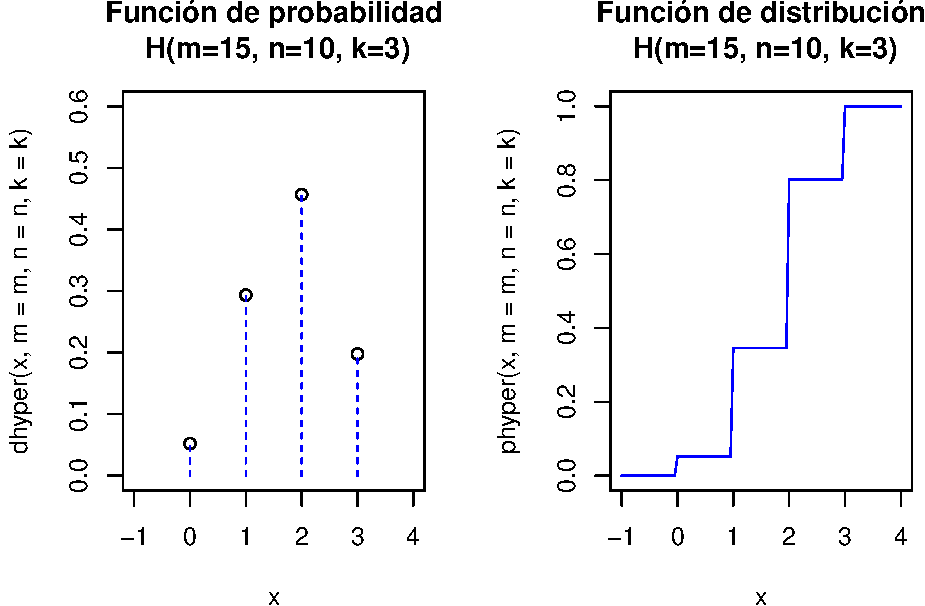
\includegraphics{curso-probabilidad-udemy_files/figure-latex/unnamed-chunk-79-1} \end{center}

\textbf{Gráficos interactivos \(H(m,n,k)\)}

Para ejecutar el siguiente gráfico interactivo, solamente tienes que cargar el paquete \texttt{shiny} en tu ordenador y luego copiar/pegar las siguientes instrucciones. De este modo podrás observar los cambios en las distribuciones variando los parámetros.

\begin{Shaded}
\begin{Highlighting}[]
\KeywordTok{fluidPage}\NormalTok{(}
\KeywordTok{fluidRow}\NormalTok{(}
  \KeywordTok{column}\NormalTok{(}\DecValTok{4}\NormalTok{,}
         \KeywordTok{sliderInput}\NormalTok{(}\StringTok{"mh"}\NormalTok{, }\DataTypeTok{label =} \StringTok{"Número de bolas blancas m"}\NormalTok{,}
              \DataTypeTok{min =} \DecValTok{1}\NormalTok{, }\DataTypeTok{max =} \DecValTok{50}\NormalTok{, }\DataTypeTok{value =}\DecValTok{15}\NormalTok{, }\DataTypeTok{step =} \DecValTok{1}\NormalTok{)),}
  \KeywordTok{column}\NormalTok{(}\DecValTok{4}\NormalTok{,}
         \KeywordTok{sliderInput}\NormalTok{(}\StringTok{"nh"}\NormalTok{, }\DataTypeTok{label =} \StringTok{"Número de bolas rojas n"}\NormalTok{,}
              \DataTypeTok{min =} \DecValTok{1}\NormalTok{, }\DataTypeTok{max =} \DecValTok{50}\NormalTok{, }\DataTypeTok{value =}\DecValTok{10}\NormalTok{ , }\DataTypeTok{step =} \DecValTok{1}\NormalTok{)),}
  \KeywordTok{column}\NormalTok{(}\DecValTok{4}\NormalTok{,}
          \KeywordTok{sliderInput}\NormalTok{(}\StringTok{"kh"}\NormalTok{, }\DataTypeTok{label =} \StringTok{"Número bolas extraídas k"}\NormalTok{,}
                     \DataTypeTok{min =} \DecValTok{1}\NormalTok{, }\DataTypeTok{max=}\DecValTok{25}\NormalTok{, }\DataTypeTok{value =} \DecValTok{3}\NormalTok{, }\DataTypeTok{step =} \DecValTok{1}\NormalTok{)}
\NormalTok{         )}
\NormalTok{  )}
\NormalTok{)}

\KeywordTok{renderPlot}\NormalTok{(\{}
\NormalTok{  m=input}\OperatorTok{$}\NormalTok{mh}
\NormalTok{  n=input}\OperatorTok{$}\NormalTok{nh}
\NormalTok{  k=input}\OperatorTok{$}\NormalTok{kh}
  \CommentTok{#n=10}
  \CommentTok{#k=3}
  \CommentTok{#m=15}
  \KeywordTok{par}\NormalTok{(}\DataTypeTok{mfrow=}\KeywordTok{c}\NormalTok{(}\DecValTok{1}\NormalTok{,}\DecValTok{2}\NormalTok{))}
\NormalTok{  a=}\KeywordTok{max}\NormalTok{(}\KeywordTok{c}\NormalTok{(}\DecValTok{0}\NormalTok{,k}\OperatorTok{-}\NormalTok{n))}
\NormalTok{  b=}\KeywordTok{min}\NormalTok{(}\KeywordTok{c}\NormalTok{(m,k))}
\NormalTok{  l=b}\OperatorTok{-}\NormalTok{a}\OperatorTok{+}\DecValTok{1}
\NormalTok{  aux=}\KeywordTok{rep}\NormalTok{(}\DecValTok{0}\NormalTok{,}\DataTypeTok{times=}\DecValTok{2}\OperatorTok{*}\NormalTok{l)}
\NormalTok{  aux[}\KeywordTok{seq}\NormalTok{(}\DecValTok{2}\NormalTok{,}\DecValTok{2}\OperatorTok{*}\NormalTok{l,}\DecValTok{2}\NormalTok{)]=}\KeywordTok{dhyper}\NormalTok{(}\KeywordTok{c}\NormalTok{(a}\OperatorTok{:}\NormalTok{b),}\DataTypeTok{m=}\NormalTok{m,}\DataTypeTok{n=}\NormalTok{n,}\DataTypeTok{k=}\NormalTok{k)}
\NormalTok{  x=a}\OperatorTok{:}\NormalTok{b}
  \KeywordTok{plot}\NormalTok{(x,}\DataTypeTok{y=}\KeywordTok{dhyper}\NormalTok{(x,}\DataTypeTok{m=}\NormalTok{m,}\DataTypeTok{n=}\NormalTok{n,}\DataTypeTok{k=}\NormalTok{k),}
       \DataTypeTok{ylim=}\KeywordTok{c}\NormalTok{(}\DecValTok{0}\NormalTok{,}\FloatTok{0.6}\NormalTok{),}\DataTypeTok{xlim=}\KeywordTok{c}\NormalTok{(a}\DecValTok{-1}\NormalTok{,b}\OperatorTok{+}\DecValTok{1}\NormalTok{),}\DataTypeTok{xlab=}\StringTok{"x"}\NormalTok{,}
       \DataTypeTok{main=}\KeywordTok{paste0}\NormalTok{(}\StringTok{"Función de probabilidad}\CharTok{\textbackslash{}n}\StringTok{ H(m="}\NormalTok{,m,}\StringTok{", n="}\NormalTok{,n,}\StringTok{", k="}\NormalTok{,k,}\StringTok{")"}\NormalTok{))}
  \KeywordTok{lines}\NormalTok{(}\DataTypeTok{x=}\KeywordTok{rep}\NormalTok{(a}\OperatorTok{:}\NormalTok{b,}\DataTypeTok{each=}\DecValTok{2}\NormalTok{),}\DataTypeTok{y=}\NormalTok{aux, }\DataTypeTok{type =} \StringTok{"h"}\NormalTok{, }\DataTypeTok{lty =} \DecValTok{2}\NormalTok{,}\DataTypeTok{col=}\StringTok{"blue"}\NormalTok{)}
  \KeywordTok{curve}\NormalTok{(}\KeywordTok{phyper}\NormalTok{(x,}\DataTypeTok{m=}\NormalTok{m,}\DataTypeTok{n=}\NormalTok{n,}\DataTypeTok{k=}\NormalTok{k),}
        \DataTypeTok{xlim=}\KeywordTok{c}\NormalTok{(a}\DecValTok{-1}\NormalTok{,b}\OperatorTok{+}\DecValTok{1}\NormalTok{),}\DataTypeTok{col=}\StringTok{"blue"}\NormalTok{,}
        \DataTypeTok{main=}\KeywordTok{paste0}\NormalTok{(}\StringTok{"Función de distribución\textbackslash{}n H(m="}\NormalTok{,m,}\StringTok{", n="}\NormalTok{,n,}\StringTok{", k="}\NormalTok{,k,}\StringTok{")"}\NormalTok{))}
  \KeywordTok{par}\NormalTok{(}\DataTypeTok{mfrow=}\KeywordTok{c}\NormalTok{(}\DecValTok{1}\NormalTok{,}\DecValTok{1}\NormalTok{))}
\NormalTok{\})}
\end{Highlighting}
\end{Shaded}

\textbf{Comparación \(H(m,n,k)\) y \(B\left(k,\frac{m}{n+m}\right)\)}

Para ejecutar el siguiente gráfico interactivo, solamente tienes que cargar el paquete \texttt{shiny} en tu ordenador y luego copiar/pegar las siguientes instrucciones. De este modo podrás observar los cambios en las distribuciones variando los parámetros.

\begin{Shaded}
\begin{Highlighting}[]
\KeywordTok{fluidPage}\NormalTok{(}
\KeywordTok{fluidRow}\NormalTok{(}
  \KeywordTok{column}\NormalTok{(}\DecValTok{4}\NormalTok{,}
         \KeywordTok{sliderInput}\NormalTok{(}\StringTok{"mh2"}\NormalTok{, }\DataTypeTok{label =} \StringTok{"Número de bolas blancas m"}\NormalTok{,}
              \DataTypeTok{min =} \DecValTok{1}\NormalTok{, }\DataTypeTok{max =} \DecValTok{50}\NormalTok{, }\DataTypeTok{value =}\DecValTok{15}\NormalTok{, }\DataTypeTok{step =} \DecValTok{1}\NormalTok{)),}
  \KeywordTok{column}\NormalTok{(}\DecValTok{4}\NormalTok{,}
         \KeywordTok{sliderInput}\NormalTok{(}\StringTok{"nh2"}\NormalTok{, }\DataTypeTok{label =} \StringTok{"Número de bolas rojas n"}\NormalTok{,}
              \DataTypeTok{min =} \DecValTok{1}\NormalTok{, }\DataTypeTok{max =} \DecValTok{50}\NormalTok{, }\DataTypeTok{value =}\DecValTok{10}\NormalTok{ , }\DataTypeTok{step =} \DecValTok{1}\NormalTok{)),}
  \KeywordTok{column}\NormalTok{(}\DecValTok{4}\NormalTok{,}
          \KeywordTok{sliderInput}\NormalTok{(}\StringTok{"kh2"}\NormalTok{, }\DataTypeTok{label =} \StringTok{"Número bolas extraídas k"}\NormalTok{,}
                     \DataTypeTok{min =} \DecValTok{1}\NormalTok{, }\DataTypeTok{max=}\DecValTok{25}\NormalTok{, }\DataTypeTok{value =} \DecValTok{3}\NormalTok{, }\DataTypeTok{step =} \DecValTok{1}\NormalTok{)}
\NormalTok{         )}
\NormalTok{  )}
\NormalTok{)}

\KeywordTok{renderPlot}\NormalTok{(\{}
\NormalTok{  m=input}\OperatorTok{$}\NormalTok{mh2}
\NormalTok{  n=input}\OperatorTok{$}\NormalTok{nh2}
\NormalTok{  k=input}\OperatorTok{$}\NormalTok{kh2}
  \CommentTok{#n=10}
  \CommentTok{#k=3}
  \CommentTok{#m=15}
\NormalTok{  pr=}\KeywordTok{round}\NormalTok{(m}\OperatorTok{/}\NormalTok{(n}\OperatorTok{+}\NormalTok{m),}\DecValTok{4}\NormalTok{)}
\NormalTok{  a=}\KeywordTok{max}\NormalTok{(}\KeywordTok{c}\NormalTok{(}\DecValTok{0}\NormalTok{,k}\OperatorTok{-}\NormalTok{n))}
\NormalTok{  b=}\KeywordTok{min}\NormalTok{(}\KeywordTok{c}\NormalTok{(m,k))}
\NormalTok{  l=b}\OperatorTok{-}\NormalTok{a}\OperatorTok{+}\DecValTok{1}
\NormalTok{  aux=}\KeywordTok{rep}\NormalTok{(}\DecValTok{0}\NormalTok{,}\DataTypeTok{times=}\DecValTok{2}\OperatorTok{*}\NormalTok{l)}
\NormalTok{  auxB=}\KeywordTok{rep}\NormalTok{(}\DecValTok{0}\NormalTok{,}\DataTypeTok{times=}\DecValTok{2}\OperatorTok{*}\NormalTok{(k}\OperatorTok{+}\DecValTok{1}\NormalTok{))}
\NormalTok{  aux[}\KeywordTok{seq}\NormalTok{(}\DecValTok{2}\NormalTok{,}\DecValTok{2}\OperatorTok{*}\NormalTok{l,}\DecValTok{2}\NormalTok{)]=}\KeywordTok{dhyper}\NormalTok{(}\KeywordTok{c}\NormalTok{(a}\OperatorTok{:}\NormalTok{b),}\DataTypeTok{m=}\NormalTok{m,}\DataTypeTok{n=}\NormalTok{n,}\DataTypeTok{k=}\NormalTok{k)}
\NormalTok{  x=a}\OperatorTok{:}\NormalTok{b}
\NormalTok{  auxB[}\KeywordTok{seq}\NormalTok{(}\DecValTok{2}\NormalTok{,}\DecValTok{2}\OperatorTok{*}\NormalTok{(k}\OperatorTok{+}\DecValTok{1}\NormalTok{),}\DecValTok{2}\NormalTok{)]=}\KeywordTok{dbinom}\NormalTok{(}\DecValTok{0}\OperatorTok{:}\NormalTok{k,k,pr)}
  \KeywordTok{par}\NormalTok{(}\DataTypeTok{mfrow=}\KeywordTok{c}\NormalTok{(}\DecValTok{1}\NormalTok{,}\DecValTok{2}\NormalTok{))}
  \KeywordTok{plot}\NormalTok{(}\DataTypeTok{x=}\KeywordTok{c}\NormalTok{(}\DecValTok{0}\OperatorTok{:}\NormalTok{k),}\DataTypeTok{y=}\KeywordTok{dbinom}\NormalTok{(}\KeywordTok{c}\NormalTok{(}\DecValTok{0}\OperatorTok{:}\NormalTok{k),}\DataTypeTok{size=}\NormalTok{k,}\DataTypeTok{prob=}\NormalTok{pr),}
       \DataTypeTok{ylim=}\KeywordTok{c}\NormalTok{(}\DecValTok{0}\NormalTok{,}\FloatTok{0.6}\NormalTok{),}\DataTypeTok{xlim=}\KeywordTok{c}\NormalTok{(}\OperatorTok{-}\DecValTok{1}\NormalTok{,k}\OperatorTok{+}\DecValTok{1}\NormalTok{),}\DataTypeTok{xlab=}\StringTok{"x"}\NormalTok{,}\DataTypeTok{ylab=}\StringTok{"Función de probabilidad"}\NormalTok{,}
       \DataTypeTok{main=}\KeywordTok{paste0}\NormalTok{(}\StringTok{"Funciones de probabilidad}\CharTok{\textbackslash{}n}\StringTok{ B(n="}\NormalTok{,n,}\StringTok{"p="}\NormalTok{,pr,}\StringTok{")  }
\StringTok{                   H(m="}\NormalTok{,m,}\StringTok{"n="}\NormalTok{, n,}\StringTok{"k="}\NormalTok{,k,}\StringTok{")"}\NormalTok{))}
  \KeywordTok{lines}\NormalTok{(}\DataTypeTok{x=}\KeywordTok{rep}\NormalTok{(}\DecValTok{0}\OperatorTok{:}\NormalTok{k,}\DataTypeTok{each=}\DecValTok{2}\NormalTok{),}\DataTypeTok{y=}\NormalTok{aux,}\DataTypeTok{pch=}\DecValTok{21}\NormalTok{, }\DataTypeTok{type =} \StringTok{"h"}\NormalTok{, }\DataTypeTok{lty =} \DecValTok{2}\NormalTok{,}\DataTypeTok{col=}\StringTok{"blue"}\NormalTok{)}
  \CommentTok{#aux=rep(0,(n+1)*2)}
  \CommentTok{#aux[seq(2,(n+1)*2,2)]=dpois(c(0:n),n*pr)}
  \KeywordTok{points}\NormalTok{(}\DataTypeTok{x=}\KeywordTok{c}\NormalTok{(a}\OperatorTok{:}\NormalTok{b),}\DataTypeTok{y=}\KeywordTok{dhyper}\NormalTok{(}\KeywordTok{c}\NormalTok{(a}\OperatorTok{:}\NormalTok{b),}\DataTypeTok{m=}\NormalTok{m,}\DataTypeTok{n=}\NormalTok{n,}\DataTypeTok{k=}\NormalTok{k),}
         \DataTypeTok{ylim=}\KeywordTok{c}\NormalTok{(}\DecValTok{0}\NormalTok{,}\FloatTok{0.6}\NormalTok{),}\DataTypeTok{xlim=}\KeywordTok{c}\NormalTok{(}\OperatorTok{-}\DecValTok{1}\NormalTok{,k}\OperatorTok{+}\DecValTok{1}\NormalTok{),}\DataTypeTok{xlab=}\StringTok{"x"}\NormalTok{,}\DataTypeTok{pch=}\DecValTok{25}\NormalTok{,}\DataTypeTok{col=}\StringTok{"red"}\NormalTok{)}
  \KeywordTok{lines}\NormalTok{(}\DataTypeTok{x=}\KeywordTok{rep}\NormalTok{(}\DecValTok{0}\OperatorTok{:}\NormalTok{(l}\DecValTok{-1}\NormalTok{),}\DataTypeTok{each=}\DecValTok{2}\NormalTok{),}\DataTypeTok{y=}\NormalTok{aux, }\DataTypeTok{type =} \StringTok{"h"}\NormalTok{, }\DataTypeTok{lty =} \DecValTok{3}\NormalTok{,}\DataTypeTok{col=}\StringTok{"red"}\NormalTok{)}
  \KeywordTok{legend}\NormalTok{(}\StringTok{"topleft"}\NormalTok{,}\DataTypeTok{legend=}\KeywordTok{c}\NormalTok{(}\StringTok{"Binomial"}\NormalTok{,}\StringTok{"Hipergeométrica"}\NormalTok{),}\DataTypeTok{col=}\KeywordTok{c}\NormalTok{(}\StringTok{"blue"}\NormalTok{,}\StringTok{"red"}\NormalTok{),}
         \DataTypeTok{pch=}\KeywordTok{c}\NormalTok{(}\DecValTok{21}\NormalTok{,}\DecValTok{25}\NormalTok{),}\DataTypeTok{lty=}\KeywordTok{c}\NormalTok{(}\DecValTok{2}\NormalTok{,}\DecValTok{3}\NormalTok{))}
  \KeywordTok{curve}\NormalTok{(}\KeywordTok{pbinom}\NormalTok{(x,}\DataTypeTok{size=}\NormalTok{k,}\DataTypeTok{p=}\NormalTok{pr),}
        \DataTypeTok{xlim=}\KeywordTok{c}\NormalTok{(}\OperatorTok{-}\DecValTok{1}\NormalTok{,k}\OperatorTok{+}\DecValTok{1}\NormalTok{), }\DataTypeTok{col=}\StringTok{"blue"}\NormalTok{, }\DataTypeTok{ylab=}\StringTok{"Función de Distribución",}
\StringTok{         main=paste0("}\NormalTok{Funciones de distribución\textbackslash{}n }\KeywordTok{B}\NormalTok{(}\StringTok{",k,"}\NormalTok{,}\StringTok{",pr,"}\NormalTok{) }
                     \KeywordTok{H}\NormalTok{(}\DataTypeTok{m=}\StringTok{",m,"}\DataTypeTok{n=}\StringTok{", n,"}\DataTypeTok{k=}\StringTok{",k,"}\NormalTok{)}\StringTok{"))}
\StringTok{  curve(phyper(x,m=m,n=n,k=k),}
\StringTok{        xlim=c(-1,k+1),col="}\NormalTok{red}\StringTok{",add=TRUE)}
\StringTok{  #if(all(c(n>=20,n*pr<10,pr<= 0.05)))\{aux_l="}\NormalTok{Condición VERDADERA}\StringTok{"\} }
\StringTok{  else \{aux_l="}\NormalTok{Condición FALSA}\StringTok{"\}}
\StringTok{  #legend("}\NormalTok{topleft}\StringTok{",legend=c(aux_l,paste0("}\DataTypeTok{n=}\StringTok{",n),paste0("}\NormalTok{n}\OperatorTok{*}\DataTypeTok{p=}\StringTok{",n*pr),}
\StringTok{  paste0("}\DataTypeTok{p=}\StringTok{",pr)),bg="}\NormalTok{transparent}\StringTok{",cex=0.5)}
\StringTok{  par(mfrow=c(1,1))}
\StringTok{\})}
\end{Highlighting}
\end{Shaded}

\textbf{Cálculos con python}

Sea \(X\) una \(H(m,n,k)\). Las funciones de \texttt{scipy.stats} cambian los parámetros de la forma siguiente:

\begin{itemize}
\tightlist
\item
  \(M\) es el número total de bolas. Con nuestra parametrización \(M=m+n\).
\item
  \(n\) es el número de bolas blancas. Con nuestra parametrización \(n=m\).
\item
  \(N\) es el número de extracciones. Con nuestra parametrización \(N=k\).
\end{itemize}

\begin{Shaded}
\begin{Highlighting}[]
\ImportTok{from}\NormalTok{ scipy.stats }\ImportTok{import}\NormalTok{ hypergeom}
\end{Highlighting}
\end{Shaded}

Los cálculos realizados anteriormente en \texttt{R} serían:

\begin{Shaded}
\begin{Highlighting}[]
\NormalTok{hypergeom.pmf(}\DecValTok{1}\NormalTok{,M}\OperatorTok{=}\DecValTok{15}\OperatorTok{+}\DecValTok{10}\NormalTok{,n}\OperatorTok{=}\DecValTok{15}\NormalTok{,N}\OperatorTok{=}\DecValTok{3}\NormalTok{)}
\end{Highlighting}
\end{Shaded}

\begin{verbatim}
## 0.29347826086956635
\end{verbatim}

\begin{Shaded}
\begin{Highlighting}[]
\NormalTok{hypergeom.cdf(}\DecValTok{1}\NormalTok{,M}\OperatorTok{=}\DecValTok{15}\OperatorTok{+}\DecValTok{10}\NormalTok{,n}\OperatorTok{=}\DecValTok{15}\NormalTok{,N}\OperatorTok{=}\DecValTok{3}\NormalTok{)}
\end{Highlighting}
\end{Shaded}

\begin{verbatim}
## 0.34565217391304481
\end{verbatim}

\begin{Shaded}
\begin{Highlighting}[]
\DecValTok{1}\OperatorTok{-}\NormalTok{hypergeom.cdf(}\DecValTok{1}\NormalTok{,M}\OperatorTok{=}\DecValTok{15}\OperatorTok{+}\DecValTok{10}\NormalTok{,n}\OperatorTok{=}\DecValTok{15}\NormalTok{,N}\OperatorTok{=}\DecValTok{3}\NormalTok{)}
\end{Highlighting}
\end{Shaded}

\begin{verbatim}
## 0.65434782608695519
\end{verbatim}

Una muestra aleatoria de este experimento sería:

\begin{Shaded}
\begin{Highlighting}[]
\NormalTok{hypergeom.rvs(M}\OperatorTok{=}\DecValTok{15}\OperatorTok{+}\DecValTok{10}\NormalTok{,n}\OperatorTok{=}\DecValTok{15}\NormalTok{,N}\OperatorTok{=}\DecValTok{3}\NormalTok{,size}\OperatorTok{=}\DecValTok{100}\NormalTok{)}
\end{Highlighting}
\end{Shaded}

\begin{verbatim}
## array([2, 1, 2, 1, 2, 2, 2, 3, 1, 2, 1, 1, 1, 1, 2, 1, 2, 2, 2, 1, 2, 1, 3,
##        1, 1, 3, 2, 1, 1, 2, 2, 2, 3, 3, 0, 3, 3, 0, 1, 2, 3, 0, 3, 1, 1, 1,
##        2, 2, 3, 1, 2, 3, 3, 2, 2, 2, 3, 2, 2, 3, 2, 3, 3, 2, 1, 1, 1, 2, 1,
##        0, 1, 2, 2, 2, 3, 3, 0, 2, 3, 2, 2, 1, 2, 2, 1, 1, 3, 2, 1, 2, 3, 2,
##        2, 1, 2, 1, 2, 0, 2, 3])
\end{verbatim}

Los gráficos de la función de probabilidad y de la función de distribución en python se realizan de la forma siguiente:

\begin{Shaded}
\begin{Highlighting}[]
\ImportTok{from}\NormalTok{ scipy.stats }\ImportTok{import}\NormalTok{ hypergeom}
\NormalTok{[M, n, N] }\OperatorTok{=}\NormalTok{ [}\DecValTok{20}\NormalTok{, }\DecValTok{7}\NormalTok{, }\DecValTok{12}\NormalTok{] }\CommentTok{##20 elementos, 7 del tipo, extraemos 12}
\NormalTok{x }\OperatorTok{=}\NormalTok{ np.arange(}\BuiltInTok{max}\NormalTok{(}\DecValTok{0}\NormalTok{, N}\OperatorTok{-}\NormalTok{M}\OperatorTok{+}\NormalTok{n),}\BuiltInTok{min}\NormalTok{(n, N))}
\NormalTok{fig }\OperatorTok{=}\NormalTok{plt.figure(figsize}\OperatorTok{=}\NormalTok{(}\DecValTok{5}\NormalTok{, }\FloatTok{2.7}\NormalTok{))}
 \OperatorTok{=}\NormalTok{ax }\OperatorTok{=}\NormalTok{ fig.add_subplot(}\DecValTok{1}\NormalTok{,}\DecValTok{2}\NormalTok{,}\DecValTok{1}\NormalTok{)}
 \OperatorTok{=}\NormalTok{ax.plot(x, hypergeom.pmf(x, M, n, N), }\StringTok{'bo'}\NormalTok{, ms}\OperatorTok{=}\DecValTok{5}\NormalTok{, label}\OperatorTok{=}\StringTok{'hypergeom pmf'}\NormalTok{)}
 \OperatorTok{=}\NormalTok{ax.vlines(x, }\DecValTok{0}\NormalTok{, hypergeom.pmf(x, M, n, N), colors}\OperatorTok{=}\StringTok{'b'}\NormalTok{, lw}\OperatorTok{=}\DecValTok{2}\NormalTok{, alpha}\OperatorTok{=}\FloatTok{0.5}\NormalTok{)}
 \OperatorTok{=}\NormalTok{ax.set_ylim([}\DecValTok{0}\NormalTok{, }\BuiltInTok{max}\NormalTok{(hypergeom.pmf(x, M, n, N))}\OperatorTok{*}\FloatTok{1.1}\NormalTok{])}
\ControlFlowTok{for}\NormalTok{ tick }\KeywordTok{in}\NormalTok{ ax.xaxis.get_major_ticks():}
   \OperatorTok{=}\NormalTok{tick.label.set_fontsize(}\DecValTok{5}\NormalTok{)}
\ControlFlowTok{for}\NormalTok{ tick }\KeywordTok{in}\NormalTok{ ax.yaxis.get_major_ticks():}
  \OperatorTok{=}\NormalTok{tick.label.set_fontsize(}\DecValTok{5}\NormalTok{) }
\NormalTok{ax }\OperatorTok{=}\NormalTok{ fig.add_subplot(}\DecValTok{1}\NormalTok{,}\DecValTok{2}\NormalTok{,}\DecValTok{2}\NormalTok{)}
 \OperatorTok{=}\NormalTok{ax.plot(x, hypergeom.cdf(x, M, n, N), }\StringTok{'bo'}\NormalTok{, ms}\OperatorTok{=}\DecValTok{5}\NormalTok{, label}\OperatorTok{=}\StringTok{'hypergeom cdf'}\NormalTok{)}
 \OperatorTok{=}\NormalTok{ax.vlines(x, }\DecValTok{0}\NormalTok{, hypergeom.cdf(x, M, n, N), colors}\OperatorTok{=}\StringTok{'b'}\NormalTok{, lw}\OperatorTok{=}\DecValTok{2}\NormalTok{, alpha}\OperatorTok{=}\FloatTok{0.5}\NormalTok{)}
\ControlFlowTok{for}\NormalTok{ tick }\KeywordTok{in}\NormalTok{ ax.xaxis.get_major_ticks():}
   \OperatorTok{=}\NormalTok{tick.label.set_fontsize(}\DecValTok{5}\NormalTok{)}
\ControlFlowTok{for}\NormalTok{ tick }\KeywordTok{in}\NormalTok{ ax.yaxis.get_major_ticks():}
   \OperatorTok{=}\NormalTok{tick.label.set_fontsize(}\DecValTok{5}\NormalTok{)}
 \OperatorTok{=}\NormalTok{fig.suptitle(}\StringTok{'Distribucion Hipergeometrica'}\NormalTok{)}
 \OperatorTok{=}\NormalTok{plt.show()}
\end{Highlighting}
\end{Shaded}

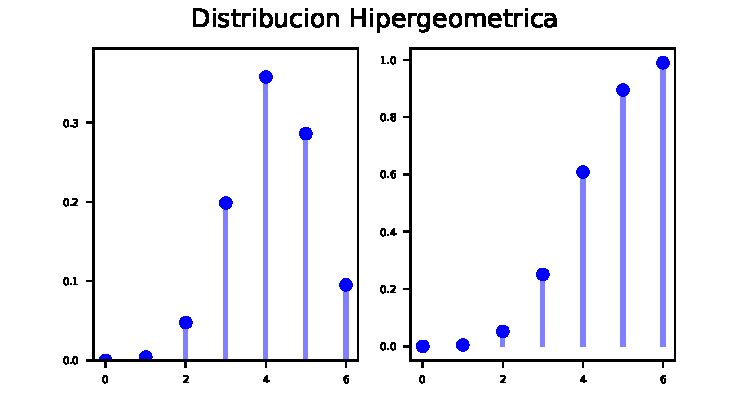
\includegraphics{curso-probabilidad-udemy_files/figure-latex/py_hyper2-1.pdf}

\hypertarget{cuantiles-de-distribuciones-notables-discretas}{%
\section{Cuantiles de distribuciones notables discretas}\label{cuantiles-de-distribuciones-notables-discretas}}

\textbf{Ejemplo}

Consideremos una v.a. \(X\) de distribución \(B(5,0.5)\).

Los cuantiles \(x_{0.3}\), \(x_{0.6}\) y \(x_{0.8}\) son los siguientes:

\begin{Shaded}
\begin{Highlighting}[]
\KeywordTok{qbinom}\NormalTok{(}\KeywordTok{c}\NormalTok{(}\FloatTok{0.3}\NormalTok{,}\FloatTok{0.6}\NormalTok{,}\FloatTok{0.8}\NormalTok{),}\DecValTok{5}\NormalTok{,}\FloatTok{0.5}\NormalTok{)}
\end{Highlighting}
\end{Shaded}

\begin{verbatim}
## [1] 2 3 3
\end{verbatim}

Calculemos a mano, el valor \(x_{0.3}\) y verifiquemos que da el mismo resultado que nos ha dado \texttt{R}.

La función de distribución de \(X\) es:
\[
\small{
F_x(x)=P(X\leq x)=
\left\{
\begin{array}{ll}
0, & x< 0, \\
0.03125, & \mbox{ si } 0 \leq x< 1, \\
0.18750, & \mbox{ si } 1 \leq x< 2, \\
0.50000, & \mbox{ si } 2 \leq x< 3, \\
0.81250, & \mbox{ si } 3 \leq x< 4, \\
0.96875, & \mbox{ si } 4 \leq x< 5, \\
1.00000, & \mbox{ si }  5\leq x. \\
\end{array}
\right.}
\]

El cuantil \(q=0.3\) es el primer valor \(x\in D_X\) tal que \(F_X(x)=P(X\leq x_{0.3})\geq 0.3.\). Mirando la expresión anterior, comprobamos que \(x_{0.3}=2\) ya que \(F_X(2)=P(X\leq 2)=0.5 \geq 0.3\).

\textbf{Ejercicio}

Calcular los cuantiles de \(0.6\) y \(0.8\) de una \(B(5,0.5).\)

\textbf{Gráfico interactivo que muestra los cuantiles de las distribuciones \(B(n,p)\) y \(Po(\lambda)\)}

Para ejecutar el siguiente gráfico interactivo, solamente tienes que cargar el paquete \texttt{shiny} en tu ordenador y luego copiar/pegar las siguientes instrucciones. De este modo podrás observar los cambios en las distribuciones variando los parámetros.

\begin{Shaded}
\begin{Highlighting}[]
\KeywordTok{fluidPage}\NormalTok{(}
\KeywordTok{fluidRow}\NormalTok{(}
  \KeywordTok{column}\NormalTok{(}\DecValTok{3}\NormalTok{,}
         \KeywordTok{sliderInput}\NormalTok{(}\StringTok{"nq"}\NormalTok{, }\DataTypeTok{label =} \StringTok{"Par. n B(n,p)"}\NormalTok{,}
              \DataTypeTok{min =} \DecValTok{1}\NormalTok{, }\DataTypeTok{max =} \DecValTok{20}\NormalTok{, }\DataTypeTok{value =}\DecValTok{10}\NormalTok{ , }\DataTypeTok{step =} \DecValTok{1}\NormalTok{)}
\NormalTok{         ),}
  \KeywordTok{column}\NormalTok{(}\DecValTok{3}\NormalTok{,}
          \KeywordTok{sliderInput}\NormalTok{(}\StringTok{"pq"}\NormalTok{, }\DataTypeTok{label =} \StringTok{"Par. p B(n,p)"}\NormalTok{,}
                     \DataTypeTok{min =} \FloatTok{0.01}\NormalTok{, }\DataTypeTok{max =} \FloatTok{0.99}\NormalTok{, }\DataTypeTok{value =} \FloatTok{0.5}\NormalTok{, }\DataTypeTok{step =} \FloatTok{0.1}\NormalTok{)}
\NormalTok{         ),}
  \KeywordTok{column}\NormalTok{(}\DecValTok{3}\NormalTok{,}
         \KeywordTok{sliderInput}\NormalTok{(}\StringTok{"qq"}\NormalTok{, }\DataTypeTok{label=}\StringTok{" Cuantil q"}\NormalTok{, }\DataTypeTok{value=}\FloatTok{0.75}\NormalTok{, }\DataTypeTok{min =} \FloatTok{0.01}\NormalTok{, }\DataTypeTok{max =} \FloatTok{0.99}\NormalTok{, }
                     \DataTypeTok{step =} \FloatTok{0.01}\NormalTok{)}
\NormalTok{         ),}
  \KeywordTok{column}\NormalTok{(}\DecValTok{3}\NormalTok{,}
         \KeywordTok{sliderInput}\NormalTok{(}\StringTok{"lq"}\NormalTok{, }\DataTypeTok{label=}\StringTok{"Par. lambda Po(lambda)"}\NormalTok{, }\DataTypeTok{value=}\DecValTok{5}\NormalTok{, }\DataTypeTok{min =} \DecValTok{1}\NormalTok{, }\DataTypeTok{max =} \DecValTok{20}\NormalTok{, }
                     \DataTypeTok{step =} \DecValTok{1}\NormalTok{)}
\NormalTok{         )}
\NormalTok{  )}
\NormalTok{)}

  
\KeywordTok{renderPlot}\NormalTok{(\{}
\NormalTok{  n=input}\OperatorTok{$}\NormalTok{nq}
\NormalTok{  p=input}\OperatorTok{$}\NormalTok{pq}
\NormalTok{  q=input}\OperatorTok{$}\NormalTok{qq}
\NormalTok{  lambda=input}\OperatorTok{$}\NormalTok{lq}
  \KeywordTok{par}\NormalTok{(}\DataTypeTok{mfrow=}\KeywordTok{c}\NormalTok{(}\DecValTok{1}\NormalTok{,}\DecValTok{2}\NormalTok{))}
  \CommentTok{#n=10;p=0.5;q=0.75;lambda=5}
  \CommentTok{#xx=c(seq(min(a,x),min(b,x),by=0.001))}
\NormalTok{  probsB=}\KeywordTok{pbinom}\NormalTok{(}\DecValTok{0}\OperatorTok{:}\NormalTok{n,n,p)}
  \KeywordTok{curve}\NormalTok{(}\KeywordTok{pbinom}\NormalTok{(x,n,p),}\DataTypeTok{xlim=}\KeywordTok{c}\NormalTok{(}\DecValTok{0}\FloatTok{-0.25}\NormalTok{,n}\FloatTok{+0.25}\NormalTok{),}\DataTypeTok{ylim=}\KeywordTok{c}\NormalTok{(}\DecValTok{0}\NormalTok{,}\KeywordTok{max}\NormalTok{(probsB}\FloatTok{+0.05}\NormalTok{,}\FloatTok{0.1}\NormalTok{)),}
        \DataTypeTok{col=}\StringTok{"blue"}\NormalTok{,}\DataTypeTok{main=}\KeywordTok{paste0}\NormalTok{(}\StringTok{"Función distribución\textbackslash{}n B(n="}\NormalTok{,n,}\StringTok{", p="}\NormalTok{,p,}\StringTok{")"}\NormalTok{),}
        \DataTypeTok{ylab=}\KeywordTok{paste0}\NormalTok{(}\StringTok{"dbinom(x,"}\NormalTok{,n,}\StringTok{", "}\NormalTok{,p,}\StringTok{")"}\NormalTok{),}\DataTypeTok{yaxt=}\StringTok{"n"}\NormalTok{)}
  \KeywordTok{segments}\NormalTok{(}\DataTypeTok{x0 =} \KeywordTok{qbinom}\NormalTok{(q,n,p),}\DataTypeTok{y0 =} \DecValTok{0}\NormalTok{,}\DataTypeTok{x1 =} \KeywordTok{qbinom}\NormalTok{(q,n,p),}\DataTypeTok{y1 =}\NormalTok{ q,}\DataTypeTok{lty=}\DecValTok{2}\NormalTok{,}\DataTypeTok{col=}\StringTok{"red"}\NormalTok{)}
  \KeywordTok{segments}\NormalTok{(}\DataTypeTok{x0 =} \KeywordTok{qbinom}\NormalTok{(q,n,p),}\DataTypeTok{y0 =}\NormalTok{ q,}\DataTypeTok{x1 =} \FloatTok{-0.25}\NormalTok{,}\DataTypeTok{y1 =}\NormalTok{ q,}\DataTypeTok{lty=}\DecValTok{2}\NormalTok{,}\DataTypeTok{col=}\StringTok{"red"}\NormalTok{)}
\NormalTok{  ytick=}\KeywordTok{c}\NormalTok{(}\FloatTok{0.0}\NormalTok{,q,}\DecValTok{1}\NormalTok{)}
  \KeywordTok{axis}\NormalTok{(}\DataTypeTok{side=}\DecValTok{2}\NormalTok{, }\DataTypeTok{at=}\NormalTok{ytick, }\DataTypeTok{labels =} \OtherTok{TRUE}\NormalTok{)}
  \KeywordTok{axis}\NormalTok{(}\DataTypeTok{side=}\DecValTok{1}\NormalTok{, }\DataTypeTok{at=}\KeywordTok{qbinom}\NormalTok{(q,n,p), }\DataTypeTok{labels =} \OtherTok{TRUE}\NormalTok{)}
  \KeywordTok{curve}\NormalTok{(}\KeywordTok{ppois}\NormalTok{(x,lambda),}\DataTypeTok{xlim=}\KeywordTok{c}\NormalTok{(}\DecValTok{0}\FloatTok{-0.25}\NormalTok{,}\FloatTok{2.5}\OperatorTok{*}\NormalTok{lambda),}\DataTypeTok{ylim=}\KeywordTok{c}\NormalTok{(}\DecValTok{0}\NormalTok{,}\DecValTok{1}\FloatTok{+0.1}\NormalTok{),}
        \DataTypeTok{col=}\StringTok{"blue"}\NormalTok{,}\DataTypeTok{main=}\KeywordTok{paste0}\NormalTok{(}\StringTok{"Función distribución }\CharTok{\textbackslash{}n}\StringTok{ Po(lambda="}\NormalTok{,lambda,}\StringTok{")"}\NormalTok{),}
        \DataTypeTok{ylab=}\KeywordTok{paste0}\NormalTok{(}\StringTok{"dpois(x, lambda"}\NormalTok{,lambda,}\StringTok{")"}\NormalTok{),}\DataTypeTok{yaxt=}\StringTok{"n"}\NormalTok{)}
  \KeywordTok{segments}\NormalTok{(}\DataTypeTok{x0 =} \KeywordTok{qpois}\NormalTok{(q,lambda),}\DataTypeTok{y0 =} \DecValTok{0}\NormalTok{,}\DataTypeTok{x1 =} \KeywordTok{qpois}\NormalTok{(q,lambda),}\DataTypeTok{y1 =}\NormalTok{ q,}\DataTypeTok{lty=}\DecValTok{2}\NormalTok{,}\DataTypeTok{col=}\StringTok{"red"}\NormalTok{)}
  \KeywordTok{segments}\NormalTok{(}\DataTypeTok{x0 =} \KeywordTok{qpois}\NormalTok{(q,lambda),}\DataTypeTok{y0 =}\NormalTok{ q,}\DataTypeTok{x1 =} \FloatTok{-0.25}\NormalTok{,}\DataTypeTok{y1 =}\NormalTok{ q,}\DataTypeTok{lty=}\DecValTok{2}\NormalTok{,}\DataTypeTok{col=}\StringTok{"red"}\NormalTok{)}
\NormalTok{  ytick=}\KeywordTok{c}\NormalTok{(}\FloatTok{0.0}\NormalTok{,q,}\DecValTok{1}\NormalTok{)}
  \KeywordTok{axis}\NormalTok{(}\DataTypeTok{side=}\DecValTok{2}\NormalTok{, }\DataTypeTok{at=}\NormalTok{ytick, }\DataTypeTok{labels =} \OtherTok{TRUE}\NormalTok{)}
  \KeywordTok{axis}\NormalTok{(}\DataTypeTok{side=}\DecValTok{1}\NormalTok{, }\DataTypeTok{at=}\KeywordTok{qpois}\NormalTok{(q,lambda), }\DataTypeTok{labels =} \OtherTok{TRUE}\NormalTok{)}
  \KeywordTok{par}\NormalTok{(}\DataTypeTok{mfrow=}\KeywordTok{c}\NormalTok{(}\DecValTok{1}\NormalTok{,}\DecValTok{1}\NormalTok{))}
\NormalTok{\})}
\end{Highlighting}
\end{Shaded}

\hypertarget{distribuciones-continuas}{%
\section{Distribuciones continuas}\label{distribuciones-continuas}}

\hypertarget{distribuciuxf3n-uniforme}{%
\subsection{Distribución uniforme}\label{distribuciuxf3n-uniforme}}

Una v.a. continua \(X\) tiene una distribución uniforme sobre el intervalo real \((a,b)\) ,con \(a<b\), si su función de densidad es

\[
f_X(x)=\left\{\begin{array}{ll}
\frac1{b-a}, & \mbox{si } a<x<b,\\ 0,  & \mbox{en cualquier otro caso.}
\end{array}
\right. 
\]

\textbf{Ejercicio}

Comprobar que el área comprendida entre \(f_X\) y la horizontal
vale 1.

El área pedida vale:
\[
\int_{-\infty}^{+\infty} f_x(x)\cdot dx=\int_{a}^{b} \frac{1}{b-a} \cdot dx=\left.\frac{x}{b-a}\right]_{x=a}^{x=b}=\frac{b}{b-a}-\frac{a}{b-a}=
\frac{b-a}{b-a}=1.
\]

Su función de distribución es:
\[
F_X(x)=\left\{\begin{array}{ll} 0,  & \mbox{si } x\leq a,\\
\frac{x-a}{b-a}, & \mbox{si } a<x<b,\\ 1,  & \mbox{si } b\leq x.
\end{array}
\right. 
\]
Efectivamente:

\begin{itemize}
\tightlist
\item
  Si \(x\leq a\), entonces
  \[F_X(x)=\int_{-\infty}^{x} f(t)\cdot dt= \int_{-\infty}^{x} 0\cdot dt.\]
\item
  Si \(a<x<b\) entonces ,
\end{itemize}

\[
\begin{array}{rl}
F_X(x)&=\displaystyle\int_{-\infty}^{x} f(t)\cdot dt= \int_{-\infty}^{a} 0\cdot dt+\int_{a}^{x} \frac1{b-a} \cdot dt\\
&= \displaystyle 0 +\left.\frac{t}{b-a}\right]_{t=a}^{t=x}= \frac{x}{b-a}-\frac{a}{b-a}=\frac{x-a}{b-a}.
\end{array}
\]
* Por último si \(x\geq b\) entonces,

\[
\begin{array}{rl}
F_X(x)&=\displaystyle\int_{-\infty}^{x} f(t) dt=\int_{a}^{b} \frac{1}{b-a} dt=
  \left.  \frac{t}{b-a} \right]_{t=a}^{t=b}
\\&=\displaystyle \frac{b}{b-a}-\frac{a}{b-a}=\frac{b-a}{b-a}=1.
\end{array}
\]

Denotaremos a la v.a. \(X\) uniforme en el intervalo \((a,b)\) por \(U(a,b)\).

\textbf{Esperanza y varianza para una v.a. \(X\) \(U(a,b)\)}

Calculemos la esperanza de \(X\):

\[
\begin{array}{rl}
E(X)&=\displaystyle\int_{-\infty}^{+\infty} x\cdot f_X(x) dx =\int_{a}^{b} x \cdot \frac{1}{b-a} dx =
\left.\frac{x^2}{2\cdot (b-a)}\right]_{x=a}^{x=b}\\
&=\displaystyle \frac{b^2}{2\cdot (b-a)}-\frac{a^2}{2\cdot (b-a)}=
\frac{b^2-a^2}{2\cdot (b-a)}=\frac{(b+a)\cdot (b-a)}{2\cdot (b-a)}=
\frac{b+a}{2}.
\end{array}
\]

De cara a calcular su varianza, calculemos primero la esperanza de \(X^2\):

\[
\begin{array}{rl}
E(X^2)&=\displaystyle\int_{-\infty}^{+\infty} x^2 f_X(x) dx=\int_{a}^{b} x^2 \frac1{b-a}
dx =\left.\frac{x^3}{3\cdot (b-a)}\right]_{x=a}^{x=b} \\
&=\displaystyle\frac{b^3-a^3}{3\cdot (b-a)}=\frac{b^2+ab+a^2}{3}.
\end{array}
\]

\textbf{Ejercicio}

\begin{itemize}
\item
  Demostrad que la igualdad \(b^3-a^3=(b-a)\cdot (b^2+ab+a^2)\) es cierta.
\item
  Utilizadla para el cálculo final del valor de \(E(X^2)\).
\end{itemize}

Calculemos \(Var(X)\).
\[
\begin{array}{rl}
Var(X)&=\displaystyle E(X^2)-(E(X))^2=\frac{b^2+ab+a^2}3-\left(\frac{b+a}2\right)^2\\&=\displaystyle
\frac{b^2+ab+a^2}{3}-\frac{b^2+2ab+a^2}{4}\\
&=\displaystyle
\frac{4\cdot (b^2+ab+a^2)-3\cdot (b^2+2ab+a^2)}{4\cdot 3}
\\
&=\displaystyle
\frac{b^2-2ab+a^2}{12}=
\frac{(b-a)^2}{12}.
\end{array}
\]

\textbf{Gráficas \(U(0,1)\)}

El código en \texttt{R} para dibujar la función de densidad y la función de distribución de una distribución \(U(0,1)\) es el siguiente:

\begin{Shaded}
\begin{Highlighting}[]
\KeywordTok{par}\NormalTok{(}\DataTypeTok{mfrow=}\KeywordTok{c}\NormalTok{(}\DecValTok{1}\NormalTok{,}\DecValTok{2}\NormalTok{))}
\NormalTok{a=}\DecValTok{0}\NormalTok{;b=}\DecValTok{1}
\KeywordTok{curve}\NormalTok{(}\KeywordTok{dunif}\NormalTok{(x,a,b),}\DataTypeTok{xlim=}\KeywordTok{c}\NormalTok{(a}\FloatTok{-0.25}\NormalTok{,b}\FloatTok{+0.25}\NormalTok{),}\DataTypeTok{ylim=}\KeywordTok{c}\NormalTok{(}\DecValTok{0}\NormalTok{,}\KeywordTok{max}\NormalTok{(}\DecValTok{1}\OperatorTok{/}\NormalTok{(b}\OperatorTok{-}\NormalTok{a)}\OperatorTok{+}\FloatTok{0.05}\NormalTok{,}\FloatTok{0.1}\NormalTok{)),}
      \DataTypeTok{col=}\StringTok{"blue"}\NormalTok{,}\DataTypeTok{main=}\KeywordTok{paste0}\NormalTok{(}\StringTok{"Función densidad  U("}\NormalTok{,a,}\StringTok{","}\NormalTok{,b,}\StringTok{")"}\NormalTok{),}
      \DataTypeTok{ylab=}\KeywordTok{paste0}\NormalTok{(}\StringTok{"dunif(x,"}\NormalTok{,a,}\StringTok{", "}\NormalTok{,b,}\StringTok{")"}\NormalTok{)}
\NormalTok{      )}
\KeywordTok{curve}\NormalTok{(}\KeywordTok{punif}\NormalTok{(x,a,b),}\DataTypeTok{xlim=}\KeywordTok{c}\NormalTok{(a}\DecValTok{-1}\NormalTok{,b}\OperatorTok{+}\DecValTok{1}\NormalTok{),}\DataTypeTok{ylim=}\KeywordTok{c}\NormalTok{(}\DecValTok{0}\NormalTok{,}\FloatTok{1.1}\NormalTok{),}
      \DataTypeTok{col=}\StringTok{"blue"}\NormalTok{,}\DataTypeTok{main=}\KeywordTok{paste0}\NormalTok{(}\StringTok{"Función de distribución U("}\NormalTok{,a,}\StringTok{","}\NormalTok{,b,}\StringTok{")"}\NormalTok{),}
      \DataTypeTok{ylab=}\KeywordTok{paste0}\NormalTok{(}\StringTok{"punif(x,"}\NormalTok{,a,}\StringTok{", "}\NormalTok{,b,}\StringTok{")"}\NormalTok{,}\DataTypeTok{cex.axis=}\FloatTok{0.8}\NormalTok{)}
\NormalTok{      )}
\KeywordTok{par}\NormalTok{(}\DataTypeTok{mfrow=}\KeywordTok{c}\NormalTok{(}\DecValTok{1}\NormalTok{,}\DecValTok{1}\NormalTok{))}
\end{Highlighting}
\end{Shaded}

\begin{center}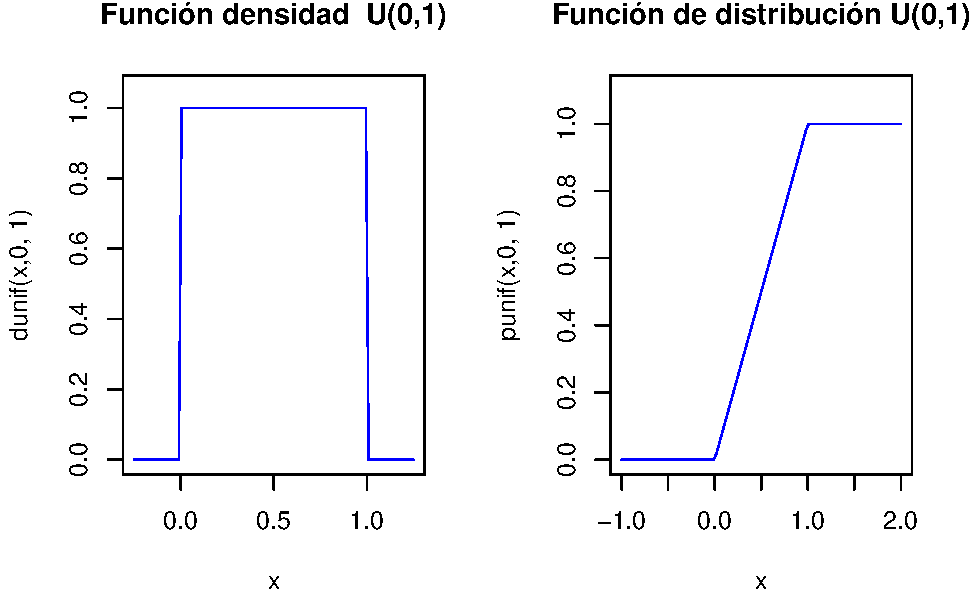
\includegraphics{curso-probabilidad-udemy_files/figure-latex/grafica_unif10_vista-1} \end{center}

\textbf{Gráficas interactivas \(U(a,b)\)}

Para ejecutar el siguiente gráfico interactivo, solamente tienes que cargar el paquete \texttt{shiny} en tu ordenador y luego copiar/pegar las siguientes instrucciones. De este modo podrás observar los cambios en las distribuciones variando los parámetros.

\begin{Shaded}
\begin{Highlighting}[]
\KeywordTok{fluidPage}\NormalTok{(}
\KeywordTok{fluidRow}\NormalTok{(}
  \KeywordTok{column}\NormalTok{(}\DecValTok{4}\NormalTok{,}
         \KeywordTok{sliderInput}\NormalTok{(}\StringTok{"a1"}\NormalTok{, }\DataTypeTok{label =} \StringTok{"Parámetro a"}\NormalTok{,}
              \DataTypeTok{min =} \DecValTok{-5}\NormalTok{, }\DataTypeTok{max =} \DecValTok{9}\NormalTok{, }\DataTypeTok{value =}\DecValTok{0}\NormalTok{ , }\DataTypeTok{step =} \FloatTok{0.1}\NormalTok{)}
\NormalTok{         ),}
  \KeywordTok{column}\NormalTok{(}\DecValTok{4}\NormalTok{,}
          \KeywordTok{sliderInput}\NormalTok{(}\StringTok{"b1"}\NormalTok{, }\DataTypeTok{label =} \StringTok{"Parámetro b"}\NormalTok{,}
                     \DataTypeTok{min =} \DecValTok{10}\NormalTok{, }\DataTypeTok{max =} \DecValTok{15}\NormalTok{, }\DataTypeTok{value =} \DecValTok{5}\NormalTok{, }\DataTypeTok{step =} \FloatTok{0.1}\NormalTok{)}
\NormalTok{         ),}
  \KeywordTok{column}\NormalTok{(}\DecValTok{4}\NormalTok{,}
         \KeywordTok{sliderInput}\NormalTok{(}\StringTok{"x1"}\NormalTok{, }\DataTypeTok{label=}\StringTok{"x"}\NormalTok{, }\DataTypeTok{value=}\DecValTok{9}\NormalTok{, }\DataTypeTok{min =} \DecValTok{-5}\NormalTok{, }\DataTypeTok{max =} \DecValTok{15}\NormalTok{, }\DataTypeTok{step =} \FloatTok{0.1}\NormalTok{)}
\NormalTok{         )}
  
\NormalTok{)}
\NormalTok{)}

\KeywordTok{renderPlot}\NormalTok{(\{}
\NormalTok{  a=input}\OperatorTok{$}\NormalTok{a1}
\NormalTok{  b=input}\OperatorTok{$}\NormalTok{b1}
\NormalTok{  x=input}\OperatorTok{$}\NormalTok{x1}
  \KeywordTok{par}\NormalTok{(}\DataTypeTok{mfrow=}\KeywordTok{c}\NormalTok{(}\DecValTok{1}\NormalTok{,}\DecValTok{2}\NormalTok{))}
  \CommentTok{#a=0;b=1;x=0.25}
\NormalTok{  xx=}\KeywordTok{c}\NormalTok{(}\KeywordTok{seq}\NormalTok{(}\KeywordTok{min}\NormalTok{(a,x),}\KeywordTok{min}\NormalTok{(b,x),}\DataTypeTok{by=}\FloatTok{0.001}\NormalTok{))}
  \KeywordTok{curve}\NormalTok{(}\KeywordTok{dunif}\NormalTok{(x,a,b),}\DataTypeTok{xlim=}\KeywordTok{c}\NormalTok{(a}\FloatTok{-0.25}\NormalTok{,b}\FloatTok{+0.25}\NormalTok{),}\DataTypeTok{ylim=}\KeywordTok{c}\NormalTok{(}\DecValTok{0}\NormalTok{,}\KeywordTok{max}\NormalTok{(}\DecValTok{1}\OperatorTok{/}\NormalTok{(b}\OperatorTok{-}\NormalTok{a)}\OperatorTok{+}\FloatTok{0.05}\NormalTok{,}\FloatTok{0.1}\NormalTok{)),}
        \DataTypeTok{col=}\StringTok{"blue"}\NormalTok{,}\DataTypeTok{main=}\KeywordTok{paste0}\NormalTok{(}\StringTok{"Función densidad U("}\NormalTok{,a,}\StringTok{","}\NormalTok{,b,}\StringTok{")"}\NormalTok{),}
  \DataTypeTok{ylab=}\KeywordTok{paste0}\NormalTok{(}\StringTok{"dunif(x,"}\NormalTok{,a,}\StringTok{", "}\NormalTok{,b,}\StringTok{")"}\NormalTok{),}\DataTypeTok{xaxt=}\StringTok{"n"}\NormalTok{)}
  \KeywordTok{axis}\NormalTok{(}\DataTypeTok{side=}\DecValTok{1}\NormalTok{, }\DataTypeTok{at=}\KeywordTok{c}\NormalTok{(a,x,b), }\DataTypeTok{labels =} \OtherTok{TRUE}\NormalTok{)}
  \KeywordTok{polygon}\NormalTok{(}\DataTypeTok{x=}\KeywordTok{c}\NormalTok{(a,xx,}\KeywordTok{min}\NormalTok{(x,b)),}\DataTypeTok{y=}\KeywordTok{c}\NormalTok{(}\DecValTok{0}\NormalTok{,}\KeywordTok{dunif}\NormalTok{(xx,a,b),}\DecValTok{0}\NormalTok{),}
          \DataTypeTok{density=}\DecValTok{20}\NormalTok{,}\DataTypeTok{col=}\StringTok{"skyblue"}\NormalTok{)}
  \KeywordTok{curve}\NormalTok{(}\KeywordTok{punif}\NormalTok{(x,a,b),}\DataTypeTok{xlim=}\KeywordTok{c}\NormalTok{(a}\DecValTok{-1}\NormalTok{,b}\OperatorTok{+}\DecValTok{1}\NormalTok{),}\DataTypeTok{ylim=}\KeywordTok{c}\NormalTok{(}\DecValTok{0}\NormalTok{,}\FloatTok{1.1}\NormalTok{),}\DataTypeTok{col=}\StringTok{"blue"}\NormalTok{,}
        \DataTypeTok{main=}\KeywordTok{paste0}\NormalTok{(}\StringTok{"Función de distribución U("}\NormalTok{,a,}\StringTok{","}\NormalTok{,b,}\StringTok{")"}\NormalTok{),}
  \DataTypeTok{ylab=}\KeywordTok{paste0}\NormalTok{(}\StringTok{"punif(x,"}\NormalTok{,a,}\StringTok{", "}\NormalTok{,b,}\StringTok{")"}\NormalTok{),}\DataTypeTok{xaxt=}\StringTok{"n"}\NormalTok{,}\DataTypeTok{yaxt=}\StringTok{"n"}\NormalTok{)}
  \KeywordTok{segments}\NormalTok{(}\DataTypeTok{x0=}\NormalTok{x,}\DataTypeTok{y0=}\DecValTok{0}\NormalTok{,}\DataTypeTok{x1=}\NormalTok{x,}\DataTypeTok{y1=}\KeywordTok{punif}\NormalTok{(x,a,b),}\DataTypeTok{col=}\StringTok{"red"}\NormalTok{,}\DataTypeTok{lty=}\DecValTok{2}\NormalTok{)}
  \KeywordTok{segments}\NormalTok{(}\DataTypeTok{x0=}\NormalTok{a}\FloatTok{-1.01}\NormalTok{,}\DataTypeTok{y0=}\KeywordTok{punif}\NormalTok{(x,a,b),}\DataTypeTok{x1=}\NormalTok{x,}\DataTypeTok{y1=}\KeywordTok{punif}\NormalTok{(x,a,b),}\DataTypeTok{col=}\StringTok{"red"}\NormalTok{,}\DataTypeTok{lty=}\DecValTok{2}\NormalTok{)}
  \KeywordTok{axis}\NormalTok{(}\DataTypeTok{side=}\DecValTok{2}\NormalTok{, }\DataTypeTok{at=}\KeywordTok{c}\NormalTok{(}\DecValTok{0}\NormalTok{,}\KeywordTok{round}\NormalTok{(}\KeywordTok{punif}\NormalTok{(x,a,b),}\DecValTok{1}\NormalTok{),}\DecValTok{2}\NormalTok{), }\DataTypeTok{labels =} \OtherTok{TRUE}\NormalTok{)}
  \KeywordTok{axis}\NormalTok{(}\DataTypeTok{side=}\DecValTok{1}\NormalTok{, }\DataTypeTok{at=}\KeywordTok{c}\NormalTok{(a,x,b), }\DataTypeTok{labels =} \OtherTok{TRUE}\NormalTok{)}
  \KeywordTok{par}\NormalTok{(}\DataTypeTok{mfrow=}\KeywordTok{c}\NormalTok{(}\DecValTok{1}\NormalTok{,}\DecValTok{1}\NormalTok{))}
\NormalTok{\})}
\end{Highlighting}
\end{Shaded}

\textbf{Transformación lineal de la v.a. uniforme}

Si \(X\) sigue una distribución \(U(a,b)\) entonces \(Z=\frac{X-a}{b-a}\) sigue una distribución \(U(0,1)\).

\textbf{Propiedad: Transformación lineal de la v.a. uniforme}

Sea \(X\) una v.a \(U(a,b)\).

Si \(scale\not=0\) y \(loc\) son dos constantes reales entonces

\begin{itemize}
\tightlist
\item
  si \(scale>0\), \(T=scale\cdot X+loc\) sigue una ley \(U(scale\cdot a +loc,scale\cdot b +loc)\)\\
\item
  si \(scale<0\), \(T=scale\cdot X+loc\) sigue una ley \(U(scale\cdot b +loc,scale\cdot a +loc)\)
\end{itemize}

\textbf{Demostración}

Supongamos que \(X\) sigue una ley \(U(a,b)\), que \(scale>0\) y que \(T=scale\cdot X+loc\). Dejamos el caso \(scale<0\) como ejercicio.

La función de distribución de \(X\) es:
\[
F_X(x)=P(X\leq x)=\left\{\begin{array}{ll} 0, & \mbox{ si } x\leq a,\\\frac{x-a}{b-a}, & \mbox{ si } a\leq x\leq b, \\1, & \mbox{ si } b\leq x.\end{array}\right.
\]

Si \(T\) vale \(T=scale\cdot X+loc\), su función de distribución será:
\[
\begin{array}{rl}
F_T(t)&=P(T\leq t)= P(scale\cdot X+ loc\leq t)= P\left(X\leq \frac{t-loc}{scale}\right)=F_X\left(\frac{t-loc}{scale}\right)\\
&=
\left\{\begin{array}{ll} 0, & \mbox{ si } \frac{t-loc}{scale}\leq a\\\frac{\frac{t-loc}{scale}-a}{b-a}, & \mbox{ si } a\leq \frac{t-loc}{scale}\leq b,\\1, & \mbox{ si } b\leq \frac{t-loc}{scale},\end{array}\right. \\ & =
\left\{\begin{array}{ll} 0, & \mbox{ si }  t\leq scale\cdot a +loc, \\
\frac{t-(scale\cdot a+loc)}{scale\cdot (b-a)}, & \mbox{ si } scale\cdot a+loc \leq t\leq scale\cdot b+loc, \\
1, & \mbox{ si } scale\cdot b+loc\leq t, \end{array}\right.\\
& = 
\left\{\begin{array}{ll} 0, & \mbox{ si }  t\leq scale\cdot a +loc, \\
\frac{t-(scale\cdot a+loc)}{scale\cdot b+loc-(scale\cdot a+loc)}, & \mbox{ si } scale\cdot a+loc \leq t\leq scale\cdot b+loc, \\
1, & \mbox{ si } scale\cdot b+loc\leq t,\end{array}\right.
\end{array}
\]
función que corresponde a la función de distribución de una v.a. \(U(scale\cdot a+loc,scale\cdot b+loc)\), como queríamos demostrar.

\textbf{Ejercicio}

Sea \(X\) una variable \(U(0,1)\) y sea \(T=scale\cdot X+loc\):

\begin{itemize}
\item
  Si \(T\) es \(U(-5,5)\) ¿qué valores toman \(scale\) y \(loc\)?
\item
  Si \(loc=-10\) y \(scale=10\) ¿qué distribución de probabilidad sigue \(T\)?
\item
  Si \(loc=0\) y \(scale=-1\) ¿qué distribución probabilidad sigue \(T\)?
\end{itemize}

\textbf{Resumen v.a con distribución uniforme, \(U(a,b)\)}

\begin{longtable}[]{@{}rl@{}}
\toprule
\begin{minipage}[b]{0.43\columnwidth}\raggedleft
Distribución uniforme\strut
\end{minipage} & \begin{minipage}[b]{0.51\columnwidth}\raggedright
\(U(a,b)\)\strut
\end{minipage}\tabularnewline
\midrule
\endhead
\begin{minipage}[t]{0.43\columnwidth}\raggedleft
Dominio\strut
\end{minipage} & \begin{minipage}[t]{0.51\columnwidth}\raggedright
\(D_X=(a,b)\)\strut
\end{minipage}\tabularnewline
\begin{minipage}[t]{0.43\columnwidth}\raggedleft
\(f_{X}(x)\)\strut
\end{minipage} & \begin{minipage}[t]{0.51\columnwidth}\raggedright
\(\left\{\begin{array}{ll}\frac1{b-a}, & \mbox{si } a<x<b,\\ 0, & \mbox{en cualquier otro caso.}\end{array} \right.\)\strut
\end{minipage}\tabularnewline
\begin{minipage}[t]{0.43\columnwidth}\raggedleft
\(F_X(x)=P(X\leq X)=\)\strut
\end{minipage} & \begin{minipage}[t]{0.51\columnwidth}\raggedright
\(\left\{\begin{array}{ll} 0, & \mbox{ si } x\leq a\\\frac{x-a}{b-a}, & \mbox{ si } a\leq x\leq b,\\1, & \mbox{ si } b\leq x.\end{array}\right.\)\strut
\end{minipage}\tabularnewline
\begin{minipage}[t]{0.43\columnwidth}\raggedleft
\(E(X)=\)\strut
\end{minipage} & \begin{minipage}[t]{0.51\columnwidth}\raggedright
\(\frac{a+b}2\)\strut
\end{minipage}\tabularnewline
\begin{minipage}[t]{0.43\columnwidth}\raggedleft
\(Var(X)=\)\strut
\end{minipage} & \begin{minipage}[t]{0.51\columnwidth}\raggedright
\(\frac{(b-a)^2}{12}\)\strut
\end{minipage}\tabularnewline
\bottomrule
\end{longtable}

\textbf{Cálculos con \texttt{R}}

Sea \(X\) una \(v.a.\) \(U(a,b)\). Las funciones \texttt{dunif(x,a,b)} y \texttt{punif(x,a,b)} calculan la función de densidad y de distribución de \(X\) en el valor \(X\). Por ejemplo, para \(a=-1\), \(b=1\) y \(x=0.5\), los valores \(f_X(x)\) y \(F_X(x)\) valen:

\begin{Shaded}
\begin{Highlighting}[]
\KeywordTok{dunif}\NormalTok{(}\DataTypeTok{x=}\FloatTok{0.5}\NormalTok{, }\DataTypeTok{min=}\OperatorTok{-}\DecValTok{1}\NormalTok{,}\DataTypeTok{max=}\DecValTok{1}\NormalTok{)}
\end{Highlighting}
\end{Shaded}

\begin{verbatim}
## [1] 0.5
\end{verbatim}

\begin{Shaded}
\begin{Highlighting}[]
\KeywordTok{punif}\NormalTok{(}\DataTypeTok{q=}\FloatTok{0.5}\NormalTok{,}\DataTypeTok{min=}\OperatorTok{-}\DecValTok{1}\NormalTok{,}\DataTypeTok{max=}\DecValTok{1}\NormalTok{)}
\end{Highlighting}
\end{Shaded}

\begin{verbatim}
## [1] 0.75
\end{verbatim}

La función \texttt{runif(n,a,b)} calcula un muestra de observaciones de tamaño \(n\) que sigan la distribución \(U(a,b)\):

\begin{Shaded}
\begin{Highlighting}[]
\KeywordTok{runif}\NormalTok{(}\DataTypeTok{n=}\DecValTok{5}\NormalTok{,}\DataTypeTok{min=}\OperatorTok{-}\DecValTok{1}\NormalTok{,}\DataTypeTok{max=}\DecValTok{1}\NormalTok{)}
\end{Highlighting}
\end{Shaded}

\begin{verbatim}
## [1] -0.5502232 -0.4271506 -0.0515360  0.8052209  0.8983523
\end{verbatim}

Por defecto, el valor de los parámetros \texttt{a} y \texttt{b} son 0 y 1, respectivamente:

\begin{Shaded}
\begin{Highlighting}[]
\KeywordTok{dunif}\NormalTok{(}\DataTypeTok{x=}\FloatTok{0.5}\NormalTok{)}
\end{Highlighting}
\end{Shaded}

\begin{verbatim}
## [1] 1
\end{verbatim}

\begin{Shaded}
\begin{Highlighting}[]
\KeywordTok{punif}\NormalTok{(}\DataTypeTok{q=}\FloatTok{0.5}\NormalTok{)}
\end{Highlighting}
\end{Shaded}

\begin{verbatim}
## [1] 0.5
\end{verbatim}

\begin{Shaded}
\begin{Highlighting}[]
\KeywordTok{runif}\NormalTok{(}\DataTypeTok{n=}\DecValTok{5}\NormalTok{)}
\end{Highlighting}
\end{Shaded}

\begin{verbatim}
## [1] 0.382302539 0.009313886 0.351767001 0.294007361 0.071581515
\end{verbatim}

\textbf{Cálculos con python}

Sea \(X\) una \(v.a.\) \(U(-1,1)\). Tomando como ``base'' la v.a. \(U(0,1)\), los parámetros \(loc\) y \(scale\) valen: \(loc=-1\) y \(scale=2,\) ya que como hemos visto \(X=2*U(0,1)-1=U(-1,1)\).

En python, hay que usar dichos parámetros para calcular la función de densidad y de distribución:

\begin{Shaded}
\begin{Highlighting}[]
\ImportTok{from}\NormalTok{ scipy.stats }\ImportTok{import}\NormalTok{ uniform}
\NormalTok{uniform.pdf(}\FloatTok{0.5}\NormalTok{,loc}\OperatorTok{=-}\DecValTok{1}\NormalTok{,scale}\OperatorTok{=}\DecValTok{2}\NormalTok{)}
\end{Highlighting}
\end{Shaded}

\begin{verbatim}
## 0.5
\end{verbatim}

\begin{Shaded}
\begin{Highlighting}[]
\NormalTok{uniform.ppf(}\FloatTok{0.5}\NormalTok{,loc}\OperatorTok{=-}\DecValTok{1}\NormalTok{,scale}\OperatorTok{=}\DecValTok{2}\NormalTok{)}
\end{Highlighting}
\end{Shaded}

\begin{verbatim}
## 0.0
\end{verbatim}

Para generar una muestra de valores aleatorios, hay que usar la función \texttt{uniform.rvs}:

\begin{Shaded}
\begin{Highlighting}[]
\NormalTok{uniform.rvs(size}\OperatorTok{=}\DecValTok{30}\NormalTok{,loc}\OperatorTok{=-}\DecValTok{1}\NormalTok{,scale}\OperatorTok{=}\DecValTok{2}\NormalTok{)}
\end{Highlighting}
\end{Shaded}

\begin{verbatim}
## array([ 0.65289599, -0.85682223,  0.03606957,  0.70835414,  0.37310414,
##        -0.91621247,  0.66120619, -0.45746474, -0.52089472,  0.63502219,
##         0.18287074, -0.92150351, -0.67308057,  0.64329807,  0.21124746,
##        -0.57233662, -0.65902493, -0.15106951,  0.68249158,  0.54293213,
##         0.49308075,  0.89919777, -0.59527182,  0.50782712,  0.12976162,
##        -0.29004971,  0.5880298 ,  0.30819297,  0.11153021, -0.21895097])
\end{verbatim}

Los valores de los parámetros por defecto son \texttt{loc=0,\ scale=1}:

\begin{Shaded}
\begin{Highlighting}[]
\NormalTok{uniform.pdf(}\FloatTok{0.5}\NormalTok{)}
\end{Highlighting}
\end{Shaded}

\begin{verbatim}
## 1.0
\end{verbatim}

\begin{Shaded}
\begin{Highlighting}[]
\NormalTok{uniform.ppf(}\FloatTok{0.5}\NormalTok{)}
\end{Highlighting}
\end{Shaded}

\begin{verbatim}
## 0.5
\end{verbatim}

\begin{Shaded}
\begin{Highlighting}[]
\NormalTok{uniform.rvs(size}\OperatorTok{=}\DecValTok{5}\NormalTok{)}
\end{Highlighting}
\end{Shaded}

\begin{verbatim}
## array([ 0.17641379,  0.88206836,  0.0193219 ,  0.323623  ,  0.36136585])
\end{verbatim}

\hypertarget{distribuciuxf3n-exponencial}{%
\subsection{Distribución exponencial}\label{distribuciuxf3n-exponencial}}

\textbf{Distribución del tiempo entre dos eventos Poisson}

Supongamos que tenemos un proceso Poisson con parámetro \(\lambda\) en una unidad de tiempo.

Dado un tiempo \(t\), definimos \(N_{t}\) como el número de eventos en el intervalo de tiempo \((0,t]\). La distribución de \(N(t)\) es una \(Po(\lambda\cdot t)\). Consideremos la v.a. \(T\) como el tiempo transcurrido entre dos eventos Poisson consecutivos.

Sea \(t>0\), entonces

\[
\begin{array}{rl}
P(T>t)&=P(\mbox{Cero eventos en el intervalo}(0,t])\\
&=P(N_{t}=0)=
         \frac{(\lambda t)^0}{0!} e^{-\lambda
         t}=e^{-\lambda t}.
\end{array}
\]

Tomando complementarios, la función de distribución de \(T\) será:
\[
F_{T}(t)= P(T\leq t)=1-P(T>t)=\left\{\begin{array}{ll} 0, &\mbox{ si } t\leq 0,\\
  1-e^{-\lambda t},& \mbox{ si } t>0,\end{array}\right.
\]

Para hallar la función de densidad de \(T\), basta derivar la expresión anterior:

\[
f_{T}(t)=\left\{\begin{array}{ll}\lambda \cdot e^{-\lambda t}, & \mbox{ si }  t>0,\\
0, & \mbox{ si } t\leq 0. \end{array}\right.
\]

Llamaremos a la variable \(T\) exponencial de parámetro \(\lambda\) y la denotaremos por \(Exp(\lambda)\).

\textbf{Propiedad de la falta de memoria}

Sea \(X\) una v.a. \(Exp(\lambda)\), entonces

\[P(X>s+t\big|X>s)=P(X>t)\mbox{  para todo } s,t\in \mathbb{R}\]

\textbf{Demostración}

Si \(X\) es una v.a. \(Exp(\lambda)\) tenemos que \(P(X>x)=1-P(X\leq x)=1-(1-e^{-\lambda\cdot x})=e^{-\lambda\cdot x}\) para todo \(x>0\).

Por tanto,
\[
\begin{array}{rl}
P(X>s+t\big|X>s) & =\frac{P(\{X>s+t\}\cap \{X>s\})}{P(X>s)}=\frac{P(X>s+t)}{P(X>s)}=\frac{e^{-\lambda\cdot (s+t)}}{e^{-\lambda\cdot s}}=
\frac{e^{-\lambda\cdot s}\cdot e^{-\lambda\cdot t} }{e^{-\lambda\cdot s}}\\ & =e^{-\lambda\cdot t}=P(X>t).
\end{array}
\]

\textbf{Ejemplo: el clásico problema del peluquero.}

Una pequeña peluquería es regentada por un único peluquero. El peluquero está esperando al próximo cliente mientras lee el periódico.

Supongamos que la v.a. \(N_T\), que representa el número de clientes que llegan en el intervalo \([0,t)\), es una \(Po(\lambda\cdot t)\) entonces la variable \(T\), tiempo entre dos clientes consecutivos, sigue una ley \(Exp(\lambda)\).

Supongamos que \(t\) se mide en horas y que \(\lambda=4\) es el promedio de clientes por hora.

Se pide:

\begin{enumerate}
\def\labelenumi{\arabic{enumi}.}
\tightlist
\item
  El tiempo esperado (en horas) y la varianza hasta el siguiente cliente.
\item
  ¿Cuál es la probabilidad de que nuestro peluquero esté sin clientes (leyendo el periódico) más de 30 minutos (0.5 horas)?
\end{enumerate}

En este ejemplo la propiedad de la pérdida de memoria significa que
por ejemplo, si el peluquero lleva ya esperando más de \(s>0.25\) (un cuarto de hora), la probabilidad de que espere \(t=1/6\) de hora más (10 minutos) no cambia sigue siendo \(P(T>0.25+1/6|T>0.25)=P(T>1/6).\)

\textbf{Solución de 1. El tiempo esperado (en horas) y la varianza hasta el siguiente cliente.}

El tiempo esperado (en horas) hasta el siguiente cliente es

\[
E(X)=\frac{1}{\lambda}=\frac{1}{4}=0.25,
\]
y la varianza es
\[
Var(X)=\frac{1}{\lambda^2}=\frac{1}{4^2}=0.0625.
\]
\textbf{Solución de 2. ¿Cuál es la probabilidad de que nuestro peluquero esté sin clientes (leyendo el periódico) más de 30 minutos (0.5 horas)?}

La probabilidad pedida vale:
\[
P(X>0.5)=1-P(X\leq 0.5)=1-(1-e^{-4\cdot 0.5 })=e^{-2}=0.1353353.
\]

Usando \texttt{R}, la probabilidad anterior puede ser calculada de la forma siguiente:

\begin{Shaded}
\begin{Highlighting}[]
\KeywordTok{pexp}\NormalTok{(}\FloatTok{0.5}\NormalTok{,}\DataTypeTok{rate=}\DecValTok{3}\NormalTok{)}
\end{Highlighting}
\end{Shaded}

\begin{verbatim}
## [1] 0.7768698
\end{verbatim}

\begin{Shaded}
\begin{Highlighting}[]
\DecValTok{1}\OperatorTok{-}\KeywordTok{pexp}\NormalTok{(}\FloatTok{0.5}\NormalTok{,}\DataTypeTok{rate=}\DecValTok{3}\NormalTok{)}
\end{Highlighting}
\end{Shaded}

\begin{verbatim}
## [1] 0.2231302
\end{verbatim}

\begin{Shaded}
\begin{Highlighting}[]
\KeywordTok{pexp}\NormalTok{(}\FloatTok{0.5}\NormalTok{,}\DataTypeTok{rate=}\DecValTok{3}\NormalTok{,}\DataTypeTok{lower.tail =} \OtherTok{FALSE}\NormalTok{)}
\end{Highlighting}
\end{Shaded}

\begin{verbatim}
## [1] 0.2231302
\end{verbatim}

\textbf{Cálculos con R}

Las funciones de densidad y de distribución de una variable exponencial de parámetro \(\lambda\) en un valor \texttt{x} se pueden obtener en \texttt{R} usando las funciones \texttt{dexp(x,lambda)} y \texttt{pexp(x,lambda)}, respectivamente. Para generar \texttt{n} valores aleatorios de una variable exponencial de parámetro \(\lambda\), hay que usar la función \texttt{rexp(n,lambda)}. Veamos un ejemplo de aplicación de las tres funciones anteriores:

\begin{Shaded}
\begin{Highlighting}[]
\KeywordTok{dexp}\NormalTok{(}\FloatTok{0.001}\NormalTok{,}\DataTypeTok{rate=}\DecValTok{3}\NormalTok{)}\CommentTok{### alerta no es una probabilidad, es una densidad y puede ser >1}
\end{Highlighting}
\end{Shaded}

\begin{verbatim}
## [1] 2.991013
\end{verbatim}

\begin{Shaded}
\begin{Highlighting}[]
\KeywordTok{pexp}\NormalTok{(}\FloatTok{0.5}\NormalTok{,}\DataTypeTok{rate=}\DecValTok{3}\NormalTok{) }\CommentTok{##P(X<0.5)}
\end{Highlighting}
\end{Shaded}

\begin{verbatim}
## [1] 0.7768698
\end{verbatim}

\begin{Shaded}
\begin{Highlighting}[]
\KeywordTok{rexp}\NormalTok{(}\DecValTok{10}\NormalTok{,}\DecValTok{3}\NormalTok{)}\CommentTok{### diez tiempos de una exponencial}
\end{Highlighting}
\end{Shaded}

\begin{verbatim}
##  [1] 0.32072389 0.57998323 0.26019628 0.48896233 0.31041354 0.11871455
##  [7] 0.10798351 0.18699902 0.10023100 0.03619832
\end{verbatim}

\textbf{Cálculos con python}

Las funciones de densidad y de distribución de una variable exponencial de parámetro \(\lambda\) en un valor \texttt{x} se pueden obtener en python usando las funciones \texttt{expon.pdf(x,scale=1/lambda)} y \texttt{expon.cdf(x,scale=1/lambda)}, respectivamente. Para generar \texttt{n} valores aleatorios de una variable exponencial de parámetro \(\lambda\), hay que usar la función \texttt{expon.rvs(scale=1/lambda,size=n)}. Veamos un ejemplo de aplicación de las tres funciones anteriores:

\begin{Shaded}
\begin{Highlighting}[]
\ImportTok{from}\NormalTok{ scipy.stats }\ImportTok{import}\NormalTok{ expon}
\NormalTok{expon.pdf(}\FloatTok{0.0001}\NormalTok{,scale}\OperatorTok{=} \FloatTok{1.}\OperatorTok{/}\DecValTok{3}\NormalTok{)}
\end{Highlighting}
\end{Shaded}

\begin{verbatim}
## 2.9991001349865014
\end{verbatim}

\begin{Shaded}
\begin{Highlighting}[]
\NormalTok{expon.cdf(}\FloatTok{0.5}\NormalTok{,scale}\OperatorTok{=} \FloatTok{1.}\OperatorTok{/}\DecValTok{3}\NormalTok{) }
\end{Highlighting}
\end{Shaded}

\begin{verbatim}
## 0.77686983985157021
\end{verbatim}

\begin{Shaded}
\begin{Highlighting}[]
\NormalTok{expon.rvs(scale}\OperatorTok{=}\FloatTok{1.}\OperatorTok{/}\DecValTok{3}\NormalTok{,size}\OperatorTok{=}\DecValTok{10}\NormalTok{)}
\end{Highlighting}
\end{Shaded}

\begin{verbatim}
## array([ 0.20450532,  0.0965351 ,  0.01170922,  0.11987187,  0.76948522,
##         0.25299269,  0.41902652,  0.37171881,  0.01288269,  0.11351932])
\end{verbatim}

\textbf{Resumen v.a con distribución exponencial, \(Exp(\lambda)\)}

\begin{longtable}[]{@{}rl@{}}
\toprule
\begin{minipage}[b]{0.47\columnwidth}\raggedleft
\(X\)\strut
\end{minipage} & \begin{minipage}[b]{0.47\columnwidth}\raggedright
\(Exp(\lambda)\)\strut
\end{minipage}\tabularnewline
\midrule
\endhead
\begin{minipage}[t]{0.47\columnwidth}\raggedleft
\(D_X=\)\strut
\end{minipage} & \begin{minipage}[t]{0.47\columnwidth}\raggedright
\((0,+\infty)\)\strut
\end{minipage}\tabularnewline
\begin{minipage}[t]{0.47\columnwidth}\raggedleft
\(f_{X}(x)=\)\strut
\end{minipage} & \begin{minipage}[t]{0.47\columnwidth}\raggedright
\(\left\{\begin{array}{ll} \lambda e^{-\lambda x}, & \mbox{ si } x>0,\\ 0, & \mbox{ si } x\leq 0. \end{array}\right.\)\strut
\end{minipage}\tabularnewline
\begin{minipage}[t]{0.47\columnwidth}\raggedleft
\(F_X(x)=P(X\leq X)=\)\strut
\end{minipage} & \begin{minipage}[t]{0.47\columnwidth}\raggedright
\(\left\{\begin{array}{ll} 0, &\mbox{si } x\leq 0,\\ 1-e^{-\lambda x},& \mbox{si } x>0.\end{array}\right.\)\strut
\end{minipage}\tabularnewline
\begin{minipage}[t]{0.47\columnwidth}\raggedleft
\(E(X)=\frac{1}{\lambda}\)\strut
\end{minipage} & \begin{minipage}[t]{0.47\columnwidth}\raggedright
\(Var(X)=\frac{1}{\lambda^2}\)\strut
\end{minipage}\tabularnewline
\bottomrule
\end{longtable}

\textbf{Gráficas de las funciones de densidad y de distribución de la variable aleatoria \(Exp(\lambda=10)\)}

\begin{Shaded}
\begin{Highlighting}[]
\NormalTok{lambda=}\DecValTok{10}
\KeywordTok{par}\NormalTok{(}\DataTypeTok{mfrow=}\KeywordTok{c}\NormalTok{(}\DecValTok{1}\NormalTok{,}\DecValTok{2}\NormalTok{))}
\KeywordTok{curve}\NormalTok{(}\KeywordTok{dexp}\NormalTok{(x,}\DataTypeTok{rate=}\NormalTok{lambda),}\DataTypeTok{xlim=}\KeywordTok{c}\NormalTok{(}\OperatorTok{-}\FloatTok{0.05}\NormalTok{,}\KeywordTok{round}\NormalTok{(}\KeywordTok{qexp}\NormalTok{(}\FloatTok{0.99}\NormalTok{,}\DataTypeTok{rate=}\NormalTok{lambda,}\DecValTok{2}\NormalTok{),}\DecValTok{2}\NormalTok{)}\OperatorTok{+}\FloatTok{0.25}\NormalTok{),}
      \DataTypeTok{ylim=}\KeywordTok{c}\NormalTok{(}\DecValTok{0}\NormalTok{,}\KeywordTok{dexp}\NormalTok{(}\DecValTok{0}\NormalTok{,lambda)}\OperatorTok{+}\FloatTok{0.1}\NormalTok{),}\DataTypeTok{col=}\StringTok{"blue"}\NormalTok{,}
      \DataTypeTok{main=}\KeywordTok{paste0}\NormalTok{(}\StringTok{"Función densidad Exp("}\NormalTok{,lambda,}\StringTok{")"}\NormalTok{),}
      \DataTypeTok{ylab=}\KeywordTok{paste0}\NormalTok{(}\StringTok{"dexp(x,rate="}\NormalTok{,lambda,}\StringTok{")"}\NormalTok{))}
\KeywordTok{curve}\NormalTok{(}\KeywordTok{pexp}\NormalTok{(x,}\DataTypeTok{rate=}\NormalTok{lambda),}\DataTypeTok{xlim=}\KeywordTok{c}\NormalTok{(}\OperatorTok{-}\FloatTok{0.05}\NormalTok{,}\KeywordTok{qexp}\NormalTok{(}\FloatTok{0.999}\NormalTok{,}\DecValTok{10}\NormalTok{)),}\DataTypeTok{ylim=}\KeywordTok{c}\NormalTok{(}\DecValTok{0}\NormalTok{,}\FloatTok{1.1}\NormalTok{),}\DataTypeTok{col=}\StringTok{"blue"}\NormalTok{,}
      \DataTypeTok{main=}\KeywordTok{paste0}\NormalTok{(}\StringTok{"Función de distribución Exp("}\NormalTok{,lambda,}\StringTok{")"}\NormalTok{),}
      \DataTypeTok{ylab=}\KeywordTok{paste0}\NormalTok{(}\StringTok{"pexp(x,rate="}\NormalTok{,lambda,}\StringTok{")"}\NormalTok{))}
\KeywordTok{par}\NormalTok{(}\DataTypeTok{mfrow=}\KeywordTok{c}\NormalTok{(}\DecValTok{1}\NormalTok{,}\DecValTok{1}\NormalTok{))}
\end{Highlighting}
\end{Shaded}

\begin{center}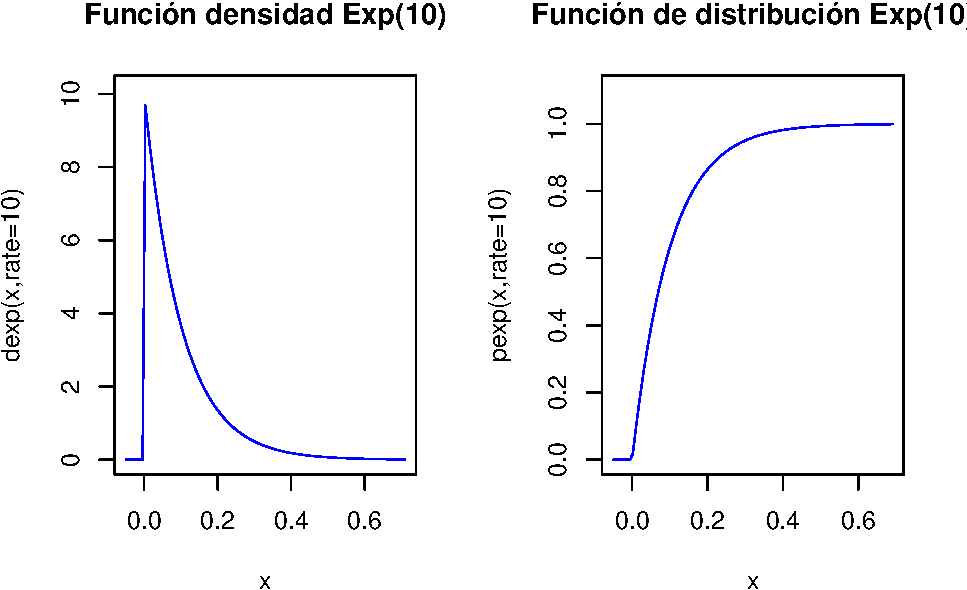
\includegraphics{curso-probabilidad-udemy_files/figure-latex/unnamed-chunk-93-1} \end{center}

\textbf{Ejercicio}

Consultad en el manual de python \href{https://docs.scipy.org/doc/scipy/reference/generated/scipy.stats.expon.html}{scipy.stats}.

Dibujad la función de densidad y de distribución de una \(Exp(\lambda=10).\)

\textbf{Gráficas interactivas de una variable \(Exp(\lambda)\)}

Para ejecutar el siguiente gráfico interactivo, solamente tienes que cargar el paquete \texttt{shiny} en tu ordenador y luego copiar/pegar las siguientes instrucciones. De este modo podrás observar los cambios en las distribuciones variando los parámetros.

\begin{Shaded}
\begin{Highlighting}[]
\KeywordTok{fluidPage}\NormalTok{(}
\KeywordTok{fluidRow}\NormalTok{(}
  \KeywordTok{column}\NormalTok{(}\DecValTok{4}\NormalTok{,}
         \KeywordTok{sliderInput}\NormalTok{(}\StringTok{"le"}\NormalTok{, }\DataTypeTok{label =} \StringTok{"lambda"}\NormalTok{,}
              \DataTypeTok{min =} \FloatTok{0.1}\NormalTok{, }\DataTypeTok{max =} \DecValTok{3}\NormalTok{, }\DataTypeTok{value =}\DecValTok{1}\NormalTok{ , }\DataTypeTok{step =} \FloatTok{0.1}\NormalTok{)}
\NormalTok{         ),}
  \KeywordTok{column}\NormalTok{(}\DecValTok{4}\NormalTok{,}
          \KeywordTok{sliderInput}\NormalTok{(}\StringTok{"xe"}\NormalTok{, }\DataTypeTok{label =} \StringTok{"X=x"}\NormalTok{,}
                     \DataTypeTok{min =} \DecValTok{0}\NormalTok{, }\DataTypeTok{max =} \DecValTok{5}\NormalTok{, }\DataTypeTok{value =} \DecValTok{5}\NormalTok{, }\DataTypeTok{step =} \FloatTok{0.1}\NormalTok{)}
\NormalTok{         ),}
  \KeywordTok{column}\NormalTok{(}\DecValTok{4}\NormalTok{,}
          \KeywordTok{sliderInput}\NormalTok{(}\StringTok{"pe"}\NormalTok{, }\DataTypeTok{label =} \StringTok{"Cuantil p"}\NormalTok{,}
                     \DataTypeTok{min =} \FloatTok{0.01}\NormalTok{, }\DataTypeTok{max =} \DecValTok{1}\NormalTok{, }\DataTypeTok{value =} \FloatTok{0.75}\NormalTok{, }\DataTypeTok{step =} \FloatTok{0.01}\NormalTok{)}
\NormalTok{         )}
\NormalTok{)}
\NormalTok{)}

\KeywordTok{renderPlot}\NormalTok{(\{}
\NormalTok{  lambda=input}\OperatorTok{$}\NormalTok{le}
\NormalTok{  p=input}\OperatorTok{$}\NormalTok{pe}
\NormalTok{  x=input}\OperatorTok{$}\NormalTok{xe}
  \CommentTok{#lambda=10;p=0.75;x=0.4}
\NormalTok{  xx=}\KeywordTok{seq}\NormalTok{(}\DecValTok{0}\NormalTok{,x,}\DataTypeTok{by=}\FloatTok{0.001}\NormalTok{)}
  \KeywordTok{par}\NormalTok{(}\DataTypeTok{mfrow=}\KeywordTok{c}\NormalTok{(}\DecValTok{1}\NormalTok{,}\DecValTok{2}\NormalTok{))}
  \KeywordTok{curve}\NormalTok{(}\KeywordTok{dexp}\NormalTok{(x,}\DataTypeTok{rate=}\NormalTok{lambda),}\DataTypeTok{xlim=}\KeywordTok{c}\NormalTok{(}\OperatorTok{-}\FloatTok{0.05}\NormalTok{,}\KeywordTok{round}\NormalTok{(}\KeywordTok{qexp}\NormalTok{(}\FloatTok{0.999}\NormalTok{,}\DataTypeTok{rate=}\NormalTok{lambda),}\DecValTok{2}\NormalTok{)),}
        \DataTypeTok{ylim=}\KeywordTok{c}\NormalTok{(}\DecValTok{0}\NormalTok{,}\KeywordTok{dexp}\NormalTok{(}\DecValTok{0}\NormalTok{,lambda)}\OperatorTok{+}\FloatTok{0.1}\NormalTok{),}\DataTypeTok{col=}\StringTok{"blue"}\NormalTok{,}
        \DataTypeTok{main=}\KeywordTok{paste0}\NormalTok{(}\StringTok{"Función densidad Exp("}\NormalTok{,lambda,}\StringTok{")"}\NormalTok{),}
  \DataTypeTok{ylab=}\KeywordTok{paste0}\NormalTok{(}\StringTok{"dexp(x,"}\NormalTok{,lambda,}\StringTok{")"}\NormalTok{),}\DataTypeTok{xaxt=}\StringTok{"n"}\NormalTok{)}
  \KeywordTok{axis}\NormalTok{(}\DataTypeTok{side=}\DecValTok{1}\NormalTok{, }\DataTypeTok{at=}\KeywordTok{c}\NormalTok{(}\DecValTok{0}\NormalTok{,x,}\KeywordTok{round}\NormalTok{(}\KeywordTok{qexp}\NormalTok{(}\FloatTok{0.999}\NormalTok{,}\DataTypeTok{rate=}\NormalTok{lambda),}\DecValTok{2}\NormalTok{)),}\DataTypeTok{cex.axis=}\FloatTok{0.8}\NormalTok{)}
  \KeywordTok{polygon}\NormalTok{(}\DataTypeTok{x=}\KeywordTok{c}\NormalTok{(}\DecValTok{0}\NormalTok{,xx,}\KeywordTok{max}\NormalTok{(x,xx)),}\DataTypeTok{y=}\KeywordTok{c}\NormalTok{(}\DecValTok{0}\NormalTok{,}\KeywordTok{dexp}\NormalTok{(xx, }\DataTypeTok{rate=}\NormalTok{lambda),}\DecValTok{0}\NormalTok{),}
          \DataTypeTok{density=}\DecValTok{20}\NormalTok{,}\DataTypeTok{col=}\StringTok{"skyblue"}\NormalTok{)}
  \KeywordTok{curve}\NormalTok{(}\KeywordTok{pexp}\NormalTok{(x,}\DataTypeTok{rate=}\NormalTok{lambda),}\DataTypeTok{xlim=}\KeywordTok{c}\NormalTok{(}\FloatTok{0.01}\NormalTok{,}\KeywordTok{qexp}\NormalTok{(}\FloatTok{0.999}\NormalTok{,}\DataTypeTok{rate=}\NormalTok{lambda)}\OperatorTok{+}\FloatTok{0.1}\NormalTok{),}
        \DataTypeTok{ylim=}\KeywordTok{c}\NormalTok{(}\DecValTok{0}\NormalTok{,}\FloatTok{1.1}\NormalTok{),}\DataTypeTok{col=}\StringTok{"blue"}\NormalTok{,}
        \DataTypeTok{main=}\KeywordTok{paste0}\NormalTok{(}\StringTok{"Función de distribución Exp("}\NormalTok{,lambda,}\StringTok{")"}\NormalTok{),}
        \DataTypeTok{ylab=}\KeywordTok{paste0}\NormalTok{(}\StringTok{"pexp(x,"}\NormalTok{,lambda,}\StringTok{")"}\NormalTok{),}\DataTypeTok{xaxt=}\StringTok{"n"}\NormalTok{,}\DataTypeTok{yaxt=}\StringTok{"n"}\NormalTok{)}
  \KeywordTok{segments}\NormalTok{(}\DataTypeTok{x0=}\KeywordTok{qexp}\NormalTok{(p,lambda),}\DataTypeTok{x1=}\KeywordTok{qexp}\NormalTok{(p,lambda),}\DataTypeTok{y0=}\DecValTok{0}\NormalTok{,}\DataTypeTok{y1=}\NormalTok{p,}\DataTypeTok{col=}\StringTok{"red"}\NormalTok{,}\DataTypeTok{lty=}\DecValTok{2}\NormalTok{)}
  \KeywordTok{segments}\NormalTok{(}\DataTypeTok{x0=}\DecValTok{0}\FloatTok{-0.05}\NormalTok{,}\DataTypeTok{y0=}\NormalTok{p,}\DataTypeTok{x1=}\KeywordTok{qexp}\NormalTok{(p,lambda),}\DataTypeTok{y1=}\NormalTok{p,}\DataTypeTok{col=}\StringTok{"red"}\NormalTok{,}\DataTypeTok{lty=}\DecValTok{2}\NormalTok{)}
  \KeywordTok{axis}\NormalTok{(}\DataTypeTok{side=}\DecValTok{2}\NormalTok{, }\DataTypeTok{at=}\KeywordTok{seq}\NormalTok{(}\DecValTok{0}\NormalTok{,}\DecValTok{1}\NormalTok{,}\FloatTok{0.1}\NormalTok{), }\DataTypeTok{labels =} \OtherTok{TRUE}\NormalTok{)}
  \KeywordTok{axis}\NormalTok{(}\DataTypeTok{side=}\DecValTok{1}\NormalTok{, }\DataTypeTok{at=}\KeywordTok{seq}\NormalTok{(}\DecValTok{0}\NormalTok{,}\KeywordTok{round}\NormalTok{(}\KeywordTok{qexp}\NormalTok{(}\FloatTok{0.999}\NormalTok{,}\DataTypeTok{rate=}\NormalTok{lambda),}\DecValTok{2}\NormalTok{),}\DataTypeTok{by=}\FloatTok{0.1}\NormalTok{), }\DataTypeTok{labels =} \OtherTok{TRUE}\NormalTok{)}
  \KeywordTok{par}\NormalTok{(}\DataTypeTok{mfrow=}\KeywordTok{c}\NormalTok{(}\DecValTok{1}\NormalTok{,}\DecValTok{1}\NormalTok{))}
\NormalTok{\})}
\end{Highlighting}
\end{Shaded}

\textbf{Ejercicio: las bombillas que no envejecen.}

Supongamos que compramos una bombilla led que promete un \textbf{valor esperado} de duración de 10000 (1.14 años) horas de funcionamiento continuo. Además, nos aseguran que la distribución de \(X\), el número de horas de funcionamiento continuo de una bombilla led, sigue una ley exponencial.

\begin{itemize}
\tightlist
\item
  Si \(X\) es \(Exp(\lambda)\) ¿cuál es el valor del parámetro \(\lambda\)?.
\item
  ¿Cuál es la probabilidad de que una bombilla led ilumine más de 2 años?
\item
  Supongamos que ya tengo una bombilla led funcionando 1 año ¿Cuál es la probabilidad de que dure dos años más?
\item
  ¿Cuál es la varianza de la duración en horas de este tipo de bombillas?
\end{itemize}

\hypertarget{distribuciuxf3n-normal-o-gaussiana}{%
\subsection{Distribución normal o Gaussiana}\label{distribuciuxf3n-normal-o-gaussiana}}

Una de las variables aleatorias continua más populares es la llamada distribución normal o \href{https://es.wikipedia.org/wiki/Distribuci\%C3\%B3n_normal}{Gaussiana}.

 \textbf{Distribución normal o de Gauss}
Diremos que una v.a. \(X\) sigue una ley normal de parámetros
\(\mu\) y \(\sigma\) y la denotaremos por \(N(\mu,\sigma)\)
si tiene por función de densidad:

\[
f_{X}(x)=\frac1{\sqrt{2\cdot\pi\cdot\sigma^2}}
e^{-\frac{1}{2}\cdot\left(\frac{x-\mu}{\sigma}\right)^2},
\]
para todo \(x\in \mathbb{R}.\)

La gráfica de esta función de densidad es conocida como \textbf{campana de Gauss.}

La v.a. normal con \(\mu=0\) y \(\sigma=1\) recibe el nombre de
normal estándar y se suele denotar por la letra \(Z\) normal \(N(0,1)\).

\begin{Shaded}
\begin{Highlighting}[]
\KeywordTok{curve}\NormalTok{(}\KeywordTok{dnorm}\NormalTok{(x),}\DataTypeTok{main=}\StringTok{"Función de densidad de una normal estándar"}\NormalTok{,}\DataTypeTok{xlim=}\KeywordTok{c}\NormalTok{(}\OperatorTok{-}\FloatTok{3.9}\NormalTok{,}\FloatTok{3.9}\NormalTok{))}
\end{Highlighting}
\end{Shaded}

\begin{center}\includegraphics{curso-probabilidad-udemy_files/figure-latex/normaldensidad1-1} \end{center}

 \textbf{Propiedades de la función de densidad de la distribución normal}

Sea \(X\) una v.a. \(N(\mu,\sigma)\) y sean \(f_{X}\) su función de densidad y \(F_X(x)=\displaystyle\int_{-\infty}^x f_X(t)\, dt\) su función de distribución. Entonces:

\begin{enumerate}
\def\labelenumi{\arabic{enumi}.}
\tightlist
\item
  La función \(f_{X}\) verifica todas las propiedades de las funciones de densidad: \(f_X(x)>0\), para todo \(x\in\mathbb{R}\) y \(\displaystyle\int_{-\infty}^\infty f_X(x)\,dx=1\).
\item
  La función \(f_X(x)\) es simétrica respecto de la recta \(x=\mu\): \(f_{X}(\mu-x)=f_{X}(\mu+x)\), para todo \(x\in\mathbb{R}\).
\item
  \(f_{X}\) tiene un único máximo absoluto en \(x=\mu\) que vale \(f_X(\mu)=\frac1{\sqrt{2\pi\sigma^2}}\).
\item
  Si \(F_{X}\) es la función de distribución de \(X\), entonces \(F_{X}(\mu+x)=1-F_{X}(\mu-x)\), para todo \(x\in\mathbb{R}\).
\item
  En particular si \(Z\) es una \(N(0,1)\) entonces \(F_{Z}(-x)=1-F_{Z}(x)\), para todo \(x\in\mathbb{R}\).
\item
  \(Z=\frac{X-\mu}{\sigma}\) es una v.a. \(N(0,1)\) y \(X=\sigma\cdot Z+\mu\) es una \(N(\mu,\sigma)\) donde \(Z\) es la normal estándar.
\item
  La función \(f_X\) es continua.
\item
  \(\lim\limits_{x\to+\infty}f(x)=\lim\limits_{x\to-\infty}f(x)=0\) es decir tiene asíntota horizontal a derecha e izquierda.
\item
  \(f\) es estrictamente creciente si \(x<\mu\) y decreciente si \(x>\mu\).
\item
  Tiene dos puntos de inflexión en \(x=\mu+\sigma\) y en \(x=\mu-\sigma\).
\end{enumerate}

\begin{center}\includegraphics{curso-probabilidad-udemy_files/figure-latex/unnamed-chunk-94-1} \end{center}

\begin{center}\includegraphics{curso-probabilidad-udemy_files/figure-latex/unnamed-chunk-95-1} \end{center}

\textbf{Función de distribución de la N(0,1)}

Su función de distribución es, como sabemos:

\[
F(x)=\displaystyle\int_{-\infty}^{x} {1\over{\sqrt{2\cdot \pi\cdot\sigma^2}}}
e^{-{1\over 2}{\left({t-\mu}\over{\sigma}\right)}^2} dt.
\]

La función \(F(x)\) no tiene ninguna expresión algebraica ``decente''. Es por esta razón, y por comodidad, que esta función está tabulada o hay que calcularla usando un software estadístico.

\textbf{Resumen v.a con distribución normal, \(N(\mu,\sigma)\)}

\begin{longtable}[]{@{}rl@{}}
\toprule
\begin{minipage}[b]{0.38\columnwidth}\raggedleft
\(X\)\strut
\end{minipage} & \begin{minipage}[b]{0.56\columnwidth}\raggedright
\(N(\mu,\sigma)\)\strut
\end{minipage}\tabularnewline
\midrule
\endhead
\begin{minipage}[t]{0.38\columnwidth}\raggedleft
\(D_X=\)\strut
\end{minipage} & \begin{minipage}[t]{0.56\columnwidth}\raggedright
\(\mathbb{R}=(-\infty,+\infty)\)\strut
\end{minipage}\tabularnewline
\begin{minipage}[t]{0.38\columnwidth}\raggedleft
\(f_{X}(x)\)\strut
\end{minipage} & \begin{minipage}[t]{0.56\columnwidth}\raggedright
\(=\frac{1}{\sqrt{2\pi\cdot\sigma^2}}\cdot e^{\frac{-(x-\mu)^2}{2\cdot \sigma^2}}\mbox{ para todo }x\in \mathbb{R}.\)\strut
\end{minipage}\tabularnewline
\begin{minipage}[t]{0.38\columnwidth}\raggedleft
\(F_X(x)=P(X\leq X)=\)\strut
\end{minipage} & \begin{minipage}[t]{0.56\columnwidth}\raggedright
Utilizad la función de \texttt{R} \texttt{pnorm(x,mean=mu,sd=sigma)} o la función correspondiente en python\strut
\end{minipage}\tabularnewline
\begin{minipage}[t]{0.38\columnwidth}\raggedleft
\(E(X)=\mu.\)\strut
\end{minipage} & \begin{minipage}[t]{0.56\columnwidth}\raggedright
\(Var(X)=\sigma^2.\)\strut
\end{minipage}\tabularnewline
\bottomrule
\end{longtable}

\textbf{Cálculos con R}

Las funciones que calculan la función de densidad y de distribución de una variable \(N(\mu,\sigma)\) en un valor \texttt{x} son \texttt{dnorm(x,mean=mu,sd=sigma)} y \texttt{pnorm(x,mean=mu,sd=sigma)}, respectivamente. Por ejemplo, para una variable \(X\sim N(\mu=1,\sigma=2)\), la función de densidad \(f_X(2)\) se puede calcular de la forma siguiente:

\begin{Shaded}
\begin{Highlighting}[]
\KeywordTok{dnorm}\NormalTok{(}\DecValTok{2}\NormalTok{,}\DataTypeTok{mean=}\DecValTok{1}\NormalTok{,}\DataTypeTok{sd=}\DecValTok{2}\NormalTok{)}
\end{Highlighting}
\end{Shaded}

\begin{verbatim}
## [1] 0.1760327
\end{verbatim}

y la función de distribución \(F_X(2) = P(X\leq 2)\) de la forma siguiente:

\begin{Shaded}
\begin{Highlighting}[]
\KeywordTok{pnorm}\NormalTok{(}\DecValTok{2}\NormalTok{,}\DataTypeTok{mean=}\DecValTok{1}\NormalTok{,}\DataTypeTok{sd=}\DecValTok{2}\NormalTok{) }
\end{Highlighting}
\end{Shaded}

\begin{verbatim}
## [1] 0.6914625
\end{verbatim}

Si queremos calcular el cuantil \(x_{q}\) de una distribución normal \(N(\mu,\sigma)\) que, recordemos es el valor que cumple que \(P(X\leq x_{q})=q\), tenemos que usar la función \texttt{qnorm(q,mean=mu,sd=sigma)}:

\begin{Shaded}
\begin{Highlighting}[]
\KeywordTok{qnorm}\NormalTok{(}\FloatTok{0.95}\NormalTok{,}\DataTypeTok{mean=}\DecValTok{1}\NormalTok{,}\DataTypeTok{sd=}\DecValTok{2}\NormalTok{)}
\end{Highlighting}
\end{Shaded}

\begin{verbatim}
## [1] 4.289707
\end{verbatim}

Para generar \texttt{n} valores aleatorios de una distribución normal \(N(\mu,\sigma)\), hay que usar la función \texttt{rnorm(n,mean=mu,sd=sigma)}:

\begin{Shaded}
\begin{Highlighting}[]
\KeywordTok{rnorm}\NormalTok{(}\DataTypeTok{n=}\DecValTok{5}\NormalTok{,}\DataTypeTok{mean=}\DecValTok{1}\NormalTok{,}\DataTypeTok{sd=}\DecValTok{2}\NormalTok{)}
\end{Highlighting}
\end{Shaded}

\begin{verbatim}
## [1] -1.7813382  0.7320555  2.7209162  2.9098518  2.5098235
\end{verbatim}

\textbf{Cálculos con python}

Para poder trabajar con una distribución normal \(N(\mu,\sigma)\) en python, tenemos que importar \texttt{norm} de \texttt{scipy.stas}. Los parámetros \(\mu\) y \(\sigma\) son \texttt{loc} y \texttt{scale}, respectivamente.

\begin{Shaded}
\begin{Highlighting}[]
\ImportTok{from}\NormalTok{ scipy.stats }\ImportTok{import}\NormalTok{ norm}
\end{Highlighting}
\end{Shaded}

Por ejemplo, para una variable \(X\sim N(\mu=1,\sigma=2)\), la función de densidad \(f_X(2)\) se puede calcular de la forma siguiente:

\begin{Shaded}
\begin{Highlighting}[]
\NormalTok{norm.pdf(}\DecValTok{2}\NormalTok{,loc}\OperatorTok{=}\DecValTok{1}\NormalTok{,scale}\OperatorTok{=}\DecValTok{2}\NormalTok{)}
\end{Highlighting}
\end{Shaded}

\begin{verbatim}
## 0.17603266338214976
\end{verbatim}

y la función de distribución \(F_X(2) = P(X\leq 2)\), de la forma siguiente:

\begin{Shaded}
\begin{Highlighting}[]
\NormalTok{norm.cdf(}\DecValTok{2}\NormalTok{,loc}\OperatorTok{=}\DecValTok{1}\NormalTok{,scale}\OperatorTok{=}\DecValTok{2}\NormalTok{)}
\end{Highlighting}
\end{Shaded}

\begin{verbatim}
## 0.69146246127401312
\end{verbatim}

Si queremos calcular el cuantil \(x_{q}\) de una distribución normal \(N(\mu,\sigma)\), tenemos que usar la función \texttt{norm.ppf(q,loc=mu,scale=sigma)}:

\begin{Shaded}
\begin{Highlighting}[]
\NormalTok{norm.ppf(}\FloatTok{0.95}\NormalTok{,loc}\OperatorTok{=}\DecValTok{1}\NormalTok{,scale}\OperatorTok{=}\DecValTok{2}\NormalTok{)}
\end{Highlighting}
\end{Shaded}

\begin{verbatim}
## 4.2897072539029448
\end{verbatim}

Para generar \texttt{n} valores aleatorios de una distribución normal \(N(\mu,\sigma)\), hay que usar la función \texttt{norm.rvs(loc=mu,scale=sigma,size=n)}:

\begin{Shaded}
\begin{Highlighting}[]
\NormalTok{norm.rvs(loc}\OperatorTok{=}\DecValTok{1}\NormalTok{,scale}\OperatorTok{=}\DecValTok{2}\NormalTok{,size}\OperatorTok{=}\DecValTok{5}\NormalTok{)}
\end{Highlighting}
\end{Shaded}

\begin{verbatim}
## array([-1.6671063 ,  4.11826416,  4.42479499, -1.77495491,  0.90060031])
\end{verbatim}

\textbf{Ejercicio}

Consultad \href{https://docs.scipy.org/doc/scipy/reference/generated/scipy.stats.norm.html}{SciPy.org} para dibujar las funciones de densidad y de distribución con python.

\textbf{Gráficas interactivas usando los parámetros de la distribución normal}

Para ejecutar el siguiente gráfico interactivo, solamente tienes que cargar el paquete \texttt{shiny} en tu ordenador y luego copiar/pegar las siguientes instrucciones. De este modo podrás observar los cambios en las distribuciones variando los parámetros.

\begin{Shaded}
\begin{Highlighting}[]
\KeywordTok{fluidPage}\NormalTok{(}
\KeywordTok{fluidRow}\NormalTok{(}
  \KeywordTok{column}\NormalTok{(}\DecValTok{3}\NormalTok{,}
         \KeywordTok{sliderInput}\NormalTok{(}\StringTok{"m1"}\NormalTok{, }\DataTypeTok{label =} \StringTok{"mu1"}\NormalTok{,}
              \DataTypeTok{min =} \DecValTok{-10}\NormalTok{, }\DataTypeTok{max =} \DecValTok{10}\NormalTok{, }\DataTypeTok{value =}\DecValTok{0}\NormalTok{ , }\DataTypeTok{step =} \FloatTok{0.05}\NormalTok{)}
\NormalTok{         ),}
  \KeywordTok{column}\NormalTok{(}\DecValTok{3}\NormalTok{,}
          \KeywordTok{sliderInput}\NormalTok{(}\StringTok{"s1"}\NormalTok{, }\DataTypeTok{label =} \StringTok{"sigma1"}\NormalTok{,}
                     \DataTypeTok{min =}\FloatTok{0.1}\NormalTok{, }\DataTypeTok{max =} \DecValTok{5}\NormalTok{, }\DataTypeTok{value =} \DecValTok{1}\NormalTok{, }\DataTypeTok{step =} \FloatTok{0.1}\NormalTok{)}
\NormalTok{         ),}
  \KeywordTok{column}\NormalTok{(}\DecValTok{3}\NormalTok{,}
         \KeywordTok{sliderInput}\NormalTok{(}\StringTok{"m2"}\NormalTok{, }\DataTypeTok{label=}\StringTok{"mu2"}\NormalTok{, }\DataTypeTok{value=}\DecValTok{4}\NormalTok{, }\DataTypeTok{min =} \DecValTok{-10}\NormalTok{, }\DataTypeTok{max =} \DecValTok{10}\NormalTok{, }\DataTypeTok{step =} \FloatTok{0.05}\NormalTok{)}
\NormalTok{         ),}
  \KeywordTok{column}\NormalTok{(}\DecValTok{3}\NormalTok{,}
          \KeywordTok{sliderInput}\NormalTok{(}\StringTok{"s2"}\NormalTok{, }\DataTypeTok{label =} \StringTok{"sigma2"}\NormalTok{,}
                     \DataTypeTok{min =}\FloatTok{0.1}\NormalTok{, }\DataTypeTok{max =} \DecValTok{5}\NormalTok{, }\DataTypeTok{value =} \DecValTok{1}\NormalTok{, }\DataTypeTok{step =} \FloatTok{0.1}\NormalTok{)}
\NormalTok{         )}
  
\NormalTok{)}
\NormalTok{)}

\KeywordTok{renderPlot}\NormalTok{(\{}
\NormalTok{  m1=input}\OperatorTok{$}\NormalTok{m1}
\NormalTok{  m2=input}\OperatorTok{$}\NormalTok{m2}
\NormalTok{  s1=input}\OperatorTok{$}\NormalTok{s1}
\NormalTok{  s2=input}\OperatorTok{$}\NormalTok{s2}
\NormalTok{  mins2=}\KeywordTok{min}\NormalTok{(}\KeywordTok{c}\NormalTok{(s1}\OperatorTok{^}\DecValTok{2}\NormalTok{,s2}\OperatorTok{^}\DecValTok{2}\NormalTok{))}
\NormalTok{m=}\KeywordTok{min}\NormalTok{(}\KeywordTok{c}\NormalTok{(}\KeywordTok{qnorm}\NormalTok{(}\FloatTok{0.01}\NormalTok{,m1,s1),}\KeywordTok{qnorm}\NormalTok{(}\FloatTok{0.01}\NormalTok{,m2,s2)))}
\NormalTok{M=}\KeywordTok{max}\NormalTok{(}\KeywordTok{c}\NormalTok{(}\KeywordTok{qnorm}\NormalTok{(}\FloatTok{0.99}\NormalTok{,m1,s1),}\KeywordTok{qnorm}\NormalTok{(}\FloatTok{0.99}\NormalTok{,m2,s2)))}

\KeywordTok{curve}\NormalTok{(}\KeywordTok{dnorm}\NormalTok{(x,m1,s1),}\DataTypeTok{xlim=}\KeywordTok{c}\NormalTok{(m,M),}\DataTypeTok{ylim=}\KeywordTok{c}\NormalTok{(}\DecValTok{0}\NormalTok{,}\DecValTok{1}\OperatorTok{/}\KeywordTok{sqrt}\NormalTok{(}\DecValTok{2}\OperatorTok{*}\NormalTok{pi}\OperatorTok{*}\NormalTok{mins2)),}\DataTypeTok{col=}\StringTok{"red"}\NormalTok{,}\DataTypeTok{lty=}\DecValTok{1}\NormalTok{)}
\KeywordTok{legend}\NormalTok{(}\StringTok{"toplef"}\NormalTok{,}\DataTypeTok{legend=}\KeywordTok{c}\NormalTok{(}\KeywordTok{expression}\NormalTok{(}\KeywordTok{N}\NormalTok{(mu[}\DecValTok{1}\NormalTok{],sigma[}\DecValTok{1}\NormalTok{])),}
                         \KeywordTok{expression}\NormalTok{(}\KeywordTok{N}\NormalTok{(mu[}\DecValTok{2}\NormalTok{],sigma[}\DecValTok{2}\NormalTok{]))),}
       \DataTypeTok{col=}\KeywordTok{c}\NormalTok{(}\StringTok{"red"}\NormalTok{,}\StringTok{"blue"}\NormalTok{),}\DataTypeTok{lty=}\KeywordTok{c}\NormalTok{(}\DecValTok{1}\NormalTok{,}\DecValTok{2}\NormalTok{))}
\KeywordTok{curve}\NormalTok{(}\KeywordTok{dnorm}\NormalTok{(x,m2,s2),}\DataTypeTok{add=}\OtherTok{TRUE}\NormalTok{,}\DataTypeTok{col=}\StringTok{"blue"}\NormalTok{,}\DataTypeTok{lty=}\DecValTok{2}\NormalTok{)}
\NormalTok{\})}
\end{Highlighting}
\end{Shaded}

\textbf{Transformaciones lineales de variables aleatorias normales}

 \textbf{Propiedad: transformación lineal la distribución normal}

Sea \(X\) una variable \(N(\mu,\sigma)\) entonces la variable \(Y=a X+b\) con
\(a\not=0,b\in\mathbb{R}\) tiene distribución \(N(a\mu+b, |a| \sigma)\)

En el caso particular en que \(a=\frac1{\sigma}\) y \(b= \frac{-\mu}{\sigma}\) obtenemos la v.a. \(Z={{X-\mu}\over {\sigma}}\), que
se distribuye según una normal estándar \(N(0,1)\), es decir \(E(X)=0\) y \(Var(X)=1\). Dicha operación se denomina estandarización de la
distribución normal.

La propiedad anterior nos permite calcular la función de distribución de cualquier v.a. \(N(\mu,\sigma)\) a partir de la función de distribución de la distribución \(Z=N(0,1)\):
\[
F_X(x)=P(X\leq x)=P\left(\frac{X-\mu}{\sigma}\leq \frac{x-\mu}{\sigma}\right)=P\left(Z\leq \frac{x-\mu}{\sigma}\right)=F_Z \left(\frac{x-\mu}{\sigma}\right).
\]
Entonces, basta conocer la manera de calcular \(F_Z\) para poder calcular \(F_X\), para \(X=N(\mu,\sigma)\), para cualquier \(\mu\) y cualquier \(\sigma>0\).

\textbf{Propiedades de la distribución normal estándar}

Sea \(Z\) una \(N(0,1)\).

En este caso, \(\mu=0\) y \(\sigma=1\). Podemos escribir algunas de las propiedades vistas para una distribución normal cualquiera de la forma siguiente:

\begin{itemize}
\tightlist
\item
  La propiedad \(f_X(\mu-x)=f_X(\mu+x)\) se traduce a \(f_Z(-x)=f_Z(x)\)
\item
  La propiedad \(F_X(\mu-x)=1-F_X(\mu+x)\) se traduce a \(F_Z(-x)=1-F(x).\)
\item
  Dado \(\delta>0\),
  \[
  P(-\delta\leq Z \leq \delta)=F_{Z}(\delta)-F_{Z}(-\delta)=F_Z(\delta)-(1-F_Z(\delta))=
  2\cdot F_Z(\delta)-1.
  \]
\end{itemize}

\textbf{Ejercicio: cálculos con la distribución normal estándar}

Sea \(Z\) una distribución \(N(0,1)\). Calcular las siguientes probabilidades en función de \(F_Z\):

\begin{itemize}
\tightlist
\item
  \(P(-4\leq Z \leq 4).\)
\item
  \(P(-2\leq Z \leq 2).\)
\item
  \(P(Z\leq -2).\)
\item
  \(P( Z \leq 2).\)
\item
  \(P( Z \geq 2).\)
\item
  \(P( Z > 2).\)
\item
  \(P( Z = 2).\)
\item
  \(P( Z \geq -2).\)
\end{itemize}

Resolución:

\begin{itemize}
\tightlist
\item
  \(P(-4\leq Z \leq 4)=F_{Z}(4)-F_{Z}(-4)=2\cdot F_Z(4)-1\).
\item
  \(P(-2\leq Z \leq 2)=F_{Z}(2)-F_{Z}(-2)=2\cdot F_Z(2)-1\).
\item
  \(P(Z\leq -2)=F_Z(-2)=1-F_Z(2)\).
\item
  \(P( Z \leq 2)=F_{Z}(2)\).
\item
  \(P( Z \geq 2)=1-P(Z<2)=1-F_{Z}(2)\).
\item
  \(P( Z > 2)=1-P(Z\leq 2)=1-F_{Z}(2)\).
\item
  \(P( Z = 2)=0\) ya que es una distribución continua.
\item
  \(P( Z \geq -2)=1-P(Z< -2)=1-F_{Z}(-2)=1-(1-F_Z(2))=F_Z(2).\)
\end{itemize}

\textbf{Cálculo de probabilidades de la distribución normal \(X=N(\mu,\sigma)\) en un intervalo usando la distribución \(Z=N(0,1)\)}

Para hallar la probabilidad de que \(X\) esté en un intervalo \((a,b)\) cualquiera, podemos usar la función de distribución de \(Z\) de la siguiente manera:
\[
\begin{array}{ll}
P(a<X<b)&=P\left(\frac{a-\mu}{\sigma}<\frac{X-\mu}{\sigma}<\frac{b-\mu}{\sigma}\right)= \\
&=P\left(\frac{a-\mu}{\sigma}<Z<\frac{b-\mu}{\sigma}\right)=F_{Z}\left(\frac{b-\mu}{\sigma}\right)-
F_{Z}\left(\frac{a-\mu}{\sigma}\right).
\end{array}
\]

Para el caso particular en que el intervalo esté centrado en la media \(\mu\), o sea existe un valor \(\delta>0\) tal que \((a,b)=(\mu-\delta,\mu+\delta)\), obtenemos:
\[
P\left(\mu-\delta\leq X \leq\mu+\delta\right)=2\cdot  F_Z\left(\frac{\delta}{\sigma}\right)-1.
\]

\textbf{Ejercicio: cálculo de probabilidades de una distribución normal}

Sea \(X\) una normal con media \(2\) y varianza \(4\). Calcular

\begin{itemize}
\tightlist
\item
  \(P(1< X< 2).\)
\item
  \(P(X>3).\)
\end{itemize}

\textbf{Solución}

La primera probabilidad se calcula de la forma siguiente:
\[
\begin{array}{ll}
P(1< X< 2)&= P\left(\frac{1-2}{2}<\frac{X-2}{2}<\frac{2-2}{2}\right)= P\left(\frac{-1}{2}<Z<0\right)\\
&= F_{Z}(0)-F_{Z}(-0.5)=\frac12-1+F_{Z}(0.5)=-\frac12+F_Z(0.5).
\end{array}
\]

La segunda probabilidad se calcular de la forma siguiente:
\[
P(X>3)=P\left(\frac{X-2}2>\frac{3-2}{2}\right)=P(Z>0.5)=1-F_{Z}(0.5).
\]

\textbf{Ejercicio}

Sea \(X\) una normal con media \(2\) y varianza \(4\). Calcular usando \texttt{R} y con python las probabilidades siguientes:

\begin{itemize}
\tightlist
\item
  \(P(1< X< 2).\)
\item
  \(P(X>3).\)
\end{itemize}

\textbf{Solución usando \texttt{R}}

\begin{Shaded}
\begin{Highlighting}[]
\KeywordTok{pnorm}\NormalTok{(}\DecValTok{2}\NormalTok{,}\DataTypeTok{mean=}\DecValTok{2}\NormalTok{,}\DataTypeTok{sd=}\DecValTok{2}\NormalTok{)}\OperatorTok{-}\KeywordTok{pnorm}\NormalTok{(}\DecValTok{1}\NormalTok{,}\DataTypeTok{mean=}\DecValTok{2}\NormalTok{,}\DataTypeTok{sd=}\DecValTok{2}\NormalTok{) }\CommentTok{#P(1< X< 2)}
\end{Highlighting}
\end{Shaded}

\begin{verbatim}
## [1] 0.1914625
\end{verbatim}

\begin{Shaded}
\begin{Highlighting}[]
\KeywordTok{pnorm}\NormalTok{(}\DecValTok{3}\NormalTok{,}\DataTypeTok{mean=}\DecValTok{2}\NormalTok{,}\DataTypeTok{sd=}\DecValTok{2}\NormalTok{,}\DataTypeTok{lower.tail =}\OtherTok{FALSE}\NormalTok{) }\CommentTok{#P(X>3)}
\end{Highlighting}
\end{Shaded}

\begin{verbatim}
## [1] 0.3085375
\end{verbatim}

\begin{Shaded}
\begin{Highlighting}[]
\DecValTok{1}\OperatorTok{-}\KeywordTok{pnorm}\NormalTok{(}\DecValTok{3}\NormalTok{,}\DataTypeTok{mean=}\DecValTok{2}\NormalTok{,}\DataTypeTok{sd=}\DecValTok{2}\NormalTok{,}\DataTypeTok{lower.tail=}\OtherTok{TRUE}\NormalTok{) }\CommentTok{#P(X>3) = 1-P(X<=3)}
\end{Highlighting}
\end{Shaded}

\begin{verbatim}
## [1] 0.3085375
\end{verbatim}

\textbf{Solución con Python}

\begin{Shaded}
\begin{Highlighting}[]
\NormalTok{norm.cdf(}\DecValTok{2}\NormalTok{,loc}\OperatorTok{=}\DecValTok{2}\NormalTok{,scale}\OperatorTok{=}\DecValTok{2}\NormalTok{)}\OperatorTok{-}\NormalTok{norm.cdf(}\DecValTok{1}\NormalTok{,loc}\OperatorTok{=}\DecValTok{2}\NormalTok{,scale}\OperatorTok{=}\DecValTok{2}\NormalTok{) }\CommentTok{#P(1< X< 2)}
\end{Highlighting}
\end{Shaded}

\begin{verbatim}
## 0.19146246127401312
\end{verbatim}

\begin{Shaded}
\begin{Highlighting}[]
\DecValTok{1}\OperatorTok{-}\NormalTok{norm.cdf(}\DecValTok{3}\NormalTok{,loc}\OperatorTok{=}\DecValTok{2}\NormalTok{,scale}\OperatorTok{=}\DecValTok{2}\NormalTok{) }\CommentTok{#P(X>3) = 1-P(X<=3)}
\end{Highlighting}
\end{Shaded}

\begin{verbatim}
## 0.30853753872598688
\end{verbatim}

\textbf{La distribución normal aproxima otras distribuciones}

En los temas que siguen veremos como, bajo determinadas condiciones,

\begin{itemize}
\tightlist
\item
  la distribución normal puede aproximar la distribución binomial,
\item
  la distribución normal puede aproximar la distribución Poisson
\item
  la distribución normal es la distribución límite de la media aritmética de una muestra de variables aleatorias.
\end{itemize}

\hypertarget{variables-aleatorias.-complementos}{%
\chapter{Variables Aleatorias. Complementos}\label{variables-aleatorias.-complementos}}

\hypertarget{momentos-de-variables-aleatorias}{%
\section{Momentos de variables aleatorias}\label{momentos-de-variables-aleatorias}}

\hypertarget{momento-de-orden-n}{%
\subsection{\texorpdfstring{Momento de orden \(n\)}{Momento de orden n}}\label{momento-de-orden-n}}

 \textbf{Definición.}
Sea \(X\) una variable aleatoria. Definimos el \textbf{momento de orden \(n\)} como
\(m_n = E\left(X^n\right)\).

 \textbf{Observación.}
El momento de orden \(1\) de una variable aleatoria es su valor medio o \(E(X)\).

Los momentos de orden \(n\) caracterizan una variable \(X\). O sea, que si conocemos todos los momentos de orden \(n\), podemos deducir cuál es la distribución de \(X\).

En general, el cálculo de los momentos de orden \(n\) para una variable \(X\) es bastante tedioso.

\textbf{Ejemplos de momentos de orden \(n\)}

\textbf{Ejemplo: momento de orden \(n\) de una variable de Bernoulli de parámetro \(p\)}

Sea \(X\) una variable de Bernoulli de parámetro \(p\). Recordemos que su función de probabilidad es:
\[
P_X(0)=q=1-p,\ p_X(1)=p.
\]
Su momento de orden \(n\) será:
\[
m_n = E\left(X^n\right)=p\cdot 1^n+(1-p)\cdot 0^n = p.
\]
En este caso, todos los momentos de orden \(n\) valen \(p\).

\textbf{Ejemplo: momento de orden \(n\) de una variable exponencial de parámetro \(\lambda\)}

Consideremos ahora una variable \(X\) exponencial de parámetro \(\lambda\).

Recordemos que su función de densidad es: \(f_X(x)=\lambda \mathrm{e}^{-\lambda x},\) para \(x\geq 0\) y \(0\), en caso contrario.

Su momento de orden \(n\) será:
\[
m_n = E\left(X^n\right)=\int_0^\infty \lambda \mathrm{e}^{-\lambda x} x^n\, dx =\frac{n!}{\lambda^n}.
\]

La expresión anterior se puede obtener integrando por partes \(n\) veces y resolviendo los límites correspondientes. Dejámos al lector los cálculos correspondientes.

Fijémonos que los momentos de orden \(n\) tienden a infinito a medida que \(n\) crece: \(\lim\limits_{n\to\infty}m_n = \lim\limits_{n\to\infty}\frac{n!}{\lambda^n}=\infty\).

\textbf{Ejemplo: momento de orden \(n\) de una variable normal de parámetros \(m=0\) y \(\sigma =1\)}

Recordemos que su función de densidad es: \(f_X(x)=\frac{1}{\sqrt{2\pi}}\mathrm{e}^{-\frac{x^2}{2}},\) para \(x\in \mathbb{R}\).

Su momento de orden 1 será la esperanza de \(X\): \(m_1 = 0\) i su momento de orden 2 será:
\(m_2 = E\left(X^2\right)=\int_{-\infty}^\infty \frac{1}{\sqrt{2\pi}}\mathrm{e}^{-\frac{x^2}{2}}\cdot x^2\, dx = 1.\)
La integral anterior se resuelve usando técnicas de integrales de dos variables.
Dicho valor también se puede obtener usando que su varianza vale 1:
\(m_2 = \mathrm{Var}(X)+E(X)^2 = \sigma^2 +0^2 = 1.\)

Los momentos de orden impar \(n\) serán cero ya que integramos una función impar:
\(m_n = E\left(X^n\right)=\int_{-\infty}^\infty \frac{1}{\sqrt{2\pi}}\mathrm{e}^{-\frac{x^2}{2}}\cdot x^n\, dx = 0.\)
O sea, si consideramos \(g(x)=\frac{1}{\sqrt{2\pi}}\mathrm{e}^{-\frac{x^2}{2}}\cdot x^n\), se verifica \(g(-x)=-g(x)\), para todo \(x\in\mathbb{R}\).

Si intentamos calcular el momento de orden 4, obtenemos:
\(m_4 = E\left(X^4\right)=\int_{-\infty}^\infty \frac{1}{\sqrt{2\pi}}\mathrm{e}^{-\frac{x^2}{2}}\cdot x^4\, dx = 3,\) usando técnicas de integración de dos variables otra vez.

\hypertarget{momento-central-de-orden-n}{%
\subsection{\texorpdfstring{Momento central de orden \(n\)}{Momento central de orden n}}\label{momento-central-de-orden-n}}

 \textbf{Definición.}
Sea \(X\) una variable aleatoria. Definimos el \textbf{momento central de orden \(n\)} como
\(\mu_n = E\left((X-\mu)^n\right)\), donde \(\mu =E(X)\) es la media o la esperanza de la variable aleatoria \(X\).

 \textbf{Observación.}
El momento central de orden \(1\) de una variable aleatoria es siempre 0:
\[
\mu_1 = E\left((X-\mu)\right)=E(X)-E(\mu)=E(X)-E(X)=0.
\]

 Observación.
El momento central de orden \(2\) de una variable aleatoria es la varianza:
\[
\mu_2 = E\left((X-\mu)^2\right):= \mathrm{Var}(X).
\]

Los momentos centrales de orden \(n\) caracterizan también una variable \(X\). O sea, que si conocemos todos los momentos centrales de orden \(n\), podemos deducir cuál es la distribución de \(X\).

 \textbf{Proposición.}
La relación que hay entre los momentos centrales y los momentos de una variable aleatoria es la siguiente:
\[
\mu_n = \sum_{k=0}^n (-1)^{n-k} \binom{n}{k} \mu^{n-k} m_k = \sum_{k=0}^n (-1)^{k} \binom{n}{k} \mu^{k} m_{n-k},
\]
donde \(\mu =E(X)\) recordemos que es la esperanza de la variable aleatoria \(X\).

\textbf{Demostración}

Recordemos la definición de momento central de orden \(n\) y desarrollemos su expresión aplicando el \textbf{binomio de Newton}:
\[
\mu_n = E\left((X-\mu)^n\right) =E\left(\sum_{k=0}^n (-1)^{n-k} \binom{n}{k} X^k\mu^{n-k}\right).
\]
Aplicando la propiedad de la esperanza que la esperanza de la suma es la suma de esperanzas, obtenemos la expresión dada por la proposición:
\[
\mu_n =\sum_{k=0}^n (-1)^{n-k} \binom{n}{k} \mu^{n-k} E\left(X^k\right) = \sum_{k=0}^n (-1)^{n-k} \binom{n}{k} \mu^{n-k} m_k.
\]

\textbf{Ejemplos de momentos centrales de orden \(n\)}

\textbf{Ejemplo: momento central de orden \(n\) de una variable de Bernoulli de parámetro \(p\)}

Sea \(X\) una variable de Bernoulli de parámetro \(p\). Recordemos que su función de probabilidad es:
\[
P_X(0)=q=1-p,\ P_X(1)=p.
\]
Usando que \(E(X)=p\), su momento central de orden \(n\) será:
\[
\mu_n = E\left((X-p)^n\right)=p\cdot (1-p)^n+(1-p)\cdot (0-p)^n = p(1-p)^n + (-1)^n (1-p) p^n.
\]

\textbf{Ejercicio}

Demostrar que la expresión anterior corresponde a un polinomio de grado \(n\).

\textbf{Ejemplo: momento central de orden \(n\) de una variable exponencial de parámetro \(\lambda\)}

Consideremos ahora una variable \(X\) exponencial de parámetro \(\lambda\).

Recordemos que su función de densidad es: \(f_X(x)=\lambda \mathrm{e}^{-\lambda x},\) para \(x\geq 0\).

Usando que \(E(X)=\frac{1}{\lambda}\), su momento central de orden \(n\) será:
\[
\mu_n = E\left(\left(X-\frac{1}{\lambda}\right)^n\right)=\int_0^\infty \lambda \mathrm{e}^{-\lambda x} \left(x-\frac{1}{\lambda}\right)^n\, dx =\frac{a_n}{\lambda^n},
\]
donde \(a_n = n!\sum\limits_{k=0}^n \frac{(-1)^k}{k!}.\)

La expresión anterior fijado \(n\) se puede obtener integrando por partes \(n\) veces y resolviendo los límites correspondientes. Dejámos al lector los cálculos correspondientes. Sin embargo, la obtención de la fórmula general para \(n\) se sale del nivel del curso.

Fijémonos que los momentos centrales de orden \(n\) también tienden a infinito a medida que \(n\) crece: \(\lim\limits_{n\to\infty}\mu_n = \lim\limits_{n\to\infty}\frac{a_n}{\lambda^n}=\infty\):
\[
\lim_{n\to\infty}\mu_n =\lim_{n\to\infty} \frac{n!\sum\limits_{k=0}^n \frac{(-1)^k}{k!}}{\lambda^n}= 
\lim_{n\to\infty}\sum\limits_{k=0}^n \frac{(-1)^k}{k!}\cdot \lim_{n\to\infty} \frac{n!}{\lambda^n}= \mathrm{e}^{-1}\cdot \infty = \infty.
\]

\textbf{Ejemplo: momento central de orden \(n\) de una variable normal de parámetros \(\mu\) y \(\sigma\)}

Recordemos que su función de densidad es: \(f_X(x)=\frac{1}{\sqrt{2\pi}\sigma}\mathrm{e}^{-\frac{(x-\mu)^2}{2\sigma^2}},\) para \(x\in \mathbb{R}\).

Su momento central de orden 2 será la varianza \(\sigma^2\): \(\mu_2 =\sigma^2.\)

Los momentos centrales de orden impar \(n\) serán cero ya que integramos una función impar respecto \(x=\mu\):
\(\mu_n = E\left((X-\mu)^n\right)=\int_{-\infty}^\infty \frac{1}{\sqrt{2\pi}\sigma}\mathrm{e}^{-\frac{(x-\mu)^2}{2\sigma^2}}\cdot (x-\mu)^n\, dx = 0.\)
O sea, si consideramos \(g(x)=\frac{1}{\sqrt{2\pi}\sigma}\mathrm{e}^{-\frac{(x-\mu)^2}{2\sigma^2}}\cdot (x-\mu)^n\), se verifica \(g(\mu-x)=-g(\mu +x)\), para todo \(x\in\mathbb{R}\).

Si intentamos calcular el momento central de orden 4, obtenemos:
\(\mu_4 = E\left((X-\mu)^4\right)=\int_{-\infty}^\infty \frac{1}{\sqrt{2\pi}\sigma}\mathrm{e}^{-\frac{(x-\mu)^2}{2\sigma^2}}\cdot (x-\mu)^4\, dx = 3\sigma^4.\) La integral anterior puede resolverse con el cambio de variable \(t=\frac{x-\mu}{\sigma}\) y usando que: \(\int_{-\infty}^\infty \frac{1}{\sqrt{2\pi}}\mathrm{e}^{-\frac{x^2}{2}}\cdot x^4\, dx = 3.\)

\hypertarget{asimetruxeda-de-una-variable-aleatoria}{%
\section{Asimetría de una variable aleatoria}\label{asimetruxeda-de-una-variable-aleatoria}}

Una variable aleatoria tiene \textbf{asimetría positiva} si su función de densidad o de probabilidad presenta una cola a la
\textbf{derecha} y \textbf{asimetría negativa}, si su función de densidad o de probabilidad presenta cola a la \textbf{izquierda}.

Por ejemplo, en la figura siguiente, vemos la gráfica de la función de probabilidad de una variable aleatoria que presenta \textbf{asimetría negativa} a la izquierda y una función de densidad de una variable aleatoria que presenta \textbf{asimetría positiva} a la derecha:

\includegraphics{curso-probabilidad-udemy_files/figure-latex/unnamed-chunk-103-1.pdf}

\textbf{¿Cómo calcular la asimetría de una variable aleatoria?}

La asimetría de una variable aleatoria \(X\) se calcula a partir de sus momentos centrales de segundo y tercer orden:
\[
\gamma_1 = E\left({\left(\frac{X-\mu}{\sigma}\right)}^3\right)=\frac{\mu_3}{\sigma^3},
\]
donde \(\mu = E(X)\) y \(\sigma^2 =\mathrm{Var}(X)\).

Dicho valor se denomina \textbf{coeficiente de asimetría de Pearson}.

Usando la relación ya vista entre los momentos centrales y los momentos, podemos expresar el \textbf{coeficiente de asimetría} en función de los momentos:
\[
\gamma_1 = \frac{m_3 -3\mu\sigma^2-\mu^3}{\sigma^3}.
\]
Dejamos al lector la comprobación de la expresión anterior.

Por tanto, una variable aleatoria \(X\) tendrá simetría positiva o a la derecha si \(\gamma_1 >0\) y tendrá asimetría negativa o a la izquierda, si \(\gamma_1 <0\).

\textbf{Ejemplo: cálculo del coeficiente de asimetría para una variable de Bernoulli de parámetro \(p\)}

Sea \(X\) una variable de Bernoulli de parámetro \(p\). Usando que \(m_n =p\), para todo \(n\) y que \(\mu_2 = \sigma^2 = p-p^2\), el coeficiente de asimetría \(\gamma_1\) será:
\[
\gamma_1 = \frac{p-3p(p-p^2)-p^3}{\sqrt{(p-p^2)^3}} = \frac{p (1-p) (1-2p)}{{\sqrt{(p-p^2)^3}}}.
\]
Por tanto, la variable de Bernoulli de parámetro \(p\) tendrá simetria negativa si \(p>\frac{1}{2}\) y positiva, si \(p<\frac{1}{2}\):

\includegraphics{curso-probabilidad-udemy_files/figure-latex/unnamed-chunk-104-1.pdf}

\textbf{Ejemplo: cálculo del coeficiente de asimetría para una variable exponencial de parámetro \(\lambda\)}

Sea \(X\) una variable exponencial de parámetro \(\lambda\).
Usando que \(\sigma^2=\frac{1}{\lambda^2}\) y \(\mu_3 =\frac{a_3}{\lambda^3}=\frac{2}{\lambda^3}\), su coeficiente de asimetría de Pearson será:
\(\gamma_1 = \frac{\frac{2}{\lambda^3}}{\frac{1}{\lambda^3}}=2.\)

Entonces presenta asimetría positiva o a la derecha tal como se observa en su función de densidad:

\includegraphics{curso-probabilidad-udemy_files/figure-latex/unnamed-chunk-105-1.pdf}

\textbf{Ejemplo: cálculo del coeficiente de asimetría para una variable normal de parámetros \(\mu\) y \(\sigma\)}

Sea \(X\) una variable aleatoria normal de parámetros \(\mu\) y \(\sigma\).

Tal como se ha indicado anteriormente, los momentos centrales de orden impar son nulos.

Por tanto, en este caso \(\mu_3=0\) y, por tanto, \(\gamma_1=0\).

Deducimos que la distribución normal es totalmente simétrica.

De hecho, usando que su función de densidad es \(f_X(x)=\frac{1}{\sqrt{2\pi}\sigma}\mathrm{e}^{-\frac{(x-\mu)^2}{2\sigma^2}},\) para \(x\in \mathbb{R}\), se puede comprobar que \(f_X(\mu-x)=f_X(\mu +x)\), o sea, tiene el eje de simetría \(x=\mu\):

\includegraphics{curso-probabilidad-udemy_files/figure-latex/unnamed-chunk-106-1.pdf}

\hypertarget{curtosis-o-apuntamiento-de-una-variable-aleatoria}{%
\section{Curtosis o apuntamiento de una variable aleatoria}\label{curtosis-o-apuntamiento-de-una-variable-aleatoria}}

La curtosis de una variable aleatoria \(X\) es una medida de cómo son las colas de su función de densidad.

Dicho en otras palabras, queremos medir de alguna manera la \emph{tendencia} que tiene la variable aleatoria a tener valores atípicos o \emph{outliers}.

La manera estándard de medir la curtosis de una variable aleatoria \(X\) es a partir de su \textbf{momento central de cuarto orden}:
\[
\gamma_2 = E\left(\left(\frac{X-\mu}{\sigma}\right)^4\right) = \frac{\mu_4}{\sigma^4},
\]
donde recordemos que \(\mu=E(X)\) y \(\sigma^2 =\mathrm{Var}(X)\).

A la expresión anterior se le denomina \textbf{medida de curtosis de Pearson}.

\begin{itemize}
\item
  Diremos que una variable aleatoria no tiene exceso de curtosis o \textbf{mesocúrtica} si \(\gamma_2 \approx 3\).
\item
  Diremos que una variable aleatoria tiene exceso positivo de curtosis o \textbf{leptocúrtica} si \(\gamma_2 >3\).
\item
  Diremos que una variable aleatoria tiene exceso negativo de curtosis o \textbf{platicúrtica} si \(\gamma_2 <3\).
\end{itemize}

\textbf{Ejemplo: cálculo del coeficiente de curtosis para una variable de Bernoulli de parámetro \(p\)}

Sea \(X\) una variable aleatoria de parámetro \(p\).

El momento central de cuarto orden de \(X\) será:
\[
\mu_4 = p (1-p)^4 +(1-p)p^4 = p (1-p) (3 p^2-3p+1).
\]
La medida de curtosis de Pearson será:
\[
\gamma_2 = \frac{p (1-p) (3 p^2-3p+1)}{p^2 (1-p)^2} = \frac{3 p^2-3p+1}{p(1-p)}.
\]
Se puede comprobar (ejercicio para el lector) que si \(p\in \left(\frac{3-\sqrt{3}}{6},\frac{3+\sqrt{3}}{6}\right)\approx (0.211,0.789)\), \(\gamma_2 <3\) y, por tanto \(X\) será platicúrtica y en caso contrario, si \(p\in \left(0,\frac{3-\sqrt{3}}{6}\right)\cup \left(\frac{3+\sqrt{3}}{6},1\right)\), \(\gamma_2 >3\) y, por tanto, \(X\) será leptocúrtica.

\textbf{Ejemplo: cálculo del coeficiente de curtosis para una variable exponencial de parámetro \(\lambda\)}

Sea \(X\) una variable exponencial de parámetro \(\lambda\).
Usando que \(\sigma^2=\frac{1}{\lambda^2}\) y \(\mu_4 =\frac{a_4}{\lambda^3}=\frac{9}{\lambda^4}\), su coeficiente de asimetría de Pearson será:
\(\gamma_2 = \frac{\frac{9}{\lambda^4}}{\frac{1}{\lambda^4}}=9.\)

Como \(\gamma_2 >3\), se trataría de una distribución leptocúrtica.

\textbf{Ejemplo: cálculo del coeficiente de curtosis para una variable normal de parámetros \(\mu\) y \(\sigma\)}

Sea \(X\) una variable aleatoria normal de parámetros \(\mu\) y \(\sigma\).

Tal como se ha indicado anteriormente, el momento central de orden 4 vale: \(\mu_4 = 3\sigma^4\).

Su coeficiente de curtosis será:
\[
\gamma_2 =\frac{\mu_4}{\sigma^4}=\frac{3\sigma^4}{\sigma^4}=3.
\]
Deducimos, por tanto, que toda distribución normal es mesocúrtica o no tiene exceso (ni positivo ni negativo) de curtosis.

\hypertarget{muxe9todos-de-transformaciuxf3n}{%
\section{Métodos de transformación}\label{muxe9todos-de-transformaciuxf3n}}

Hemos visto anteriormente que el cálculo de los \textbf{momentos} o los \textbf{momentos centrados} de una variable aleatoria \(X\) puede ser muy complicado y muy tedioso.

Por dicho motivo, vamos a introducir un conjunto de funciones que nos permitirán calcular los \textbf{momentos} de la variable \(X\) de forma relativamente sencilla.

\hypertarget{funciuxf3n-generatriz-de-momentos}{%
\subsection{Función generatriz de momentos}\label{funciuxf3n-generatriz-de-momentos}}

\textbf{Definición de función generatriz de momentos:}
Sea \(X\) una variable aleatoria \(X\) con función de probabilidad \(P_X\) en el caso discreto o función
de densidad \(f_X\) en el caso continuo.

Sea \(t\in\mathbb{R}\) un valor real cualquiera.

Definimos la función generatriz de momentos \(m_X(t)\) en el valor \(t\) como: \(m_X(t)=E\left(\mathrm{e}^{tX}\right).\)

\textbf{Ejemplo: cálculo de la función generatriz de momentos para una variable de Bernoulli de parámetro \(p\)}

Sea \(X\) una variable aleatoria de Bernoulli de parámetro \(p\). Recordemos que su función de probabilidad es:
\[
P_X(0)=q=1-p,\ p_X(1)=p.
\]
Su función generatriz de momentos será:
\[
m_X (t)=E\left(\mathrm{e}^{tX}\right) =p\mathrm{e}^{t\cdot 1}+(1-p)\mathrm{e}^{t\cdot 0}=p\mathrm{e}^t+(1-p)=1+p\left(\mathrm{e}^t -1 \right).
\]

\textbf{Ejemplo: cálculo de la función generatriz de momentos para una variable exponencial de parámetro \(\lambda\)}

Sea \(X\) una variable aleatoria exponencial de parámetro \(\lambda\). Recordemos que su función de densidad es: \(f_X(x)=\lambda \mathrm{e}^{-\lambda x},\) para \(x\geq 0\) y \(0\), en caso contrario.

Su función generatriz de momentos será:
\[
m_X (t)=E\left(\mathrm{e}^{tX}\right)=\int_0^\infty \mathrm{e}^{t x}\lambda \mathrm{e}^{-\lambda x}\, dx = \lambda \int_0^\infty\mathrm{e}^{(t-\lambda)x}\, dx = \lambda\left[\frac{\mathrm{e}^{(t-\lambda)x}}{t-\lambda}\right]_{x=0}^{x=\infty} = \frac{\lambda}{\lambda -t},\ \mbox{si } t<\lambda. 
\]
En este caso vemos que el dominio de la función generatriz de momentos \(m_X\) es \((-\infty,\lambda)\), ya que si \(t\geq \lambda\), la integral anterior no es convergente.

Fijémonos por lo que vendrá más adelante que, como \(\lambda >0\), el valor \(0\) pertenece al dominio de \(m_X\).

\textbf{Ejemplo: cálculo de la función generatriz de momentos para una variable normal de parámetros \(\mu\) y \(\sigma\)}

Sea \(X\) una variable normal de parámetros \(\mu\) y \(\sigma\).

Recordemos que su función de densidad es: \(f_X(x)=\frac{1}{\sqrt{2\pi}\sigma}\mathrm{e}^{-\frac{(x-\mu)^2}{2\sigma^2}},\) para \(x\in \mathbb{R}\).

Su función generatriz de momentos será:

\[
\begin{array}{rl}
m_X (t) & =E\left(\mathrm{e}^{tX}\right)=\displaystyle\int_{-\infty}^\infty \mathrm{e}^{tx}\frac{1}{\sqrt{2\pi}\sigma}\mathrm{e}^{-\frac{(x-\mu)^2}{2\sigma^2}}\, dx = \frac{1}{\sqrt{2\pi}\sigma} \int_{-\infty}^\infty \mathrm{e}^{tx-\frac{(x-\mu)^2}{2\sigma^2}}\, dx \\[1ex]  & =  \displaystyle\frac{1}{\sqrt{2\pi}\sigma} \int_{-\infty}^\infty \mathrm{e}^{-\frac{1}{2\sigma^2}\left((x-(\sigma^2 t+\mu))^2-2\sigma^2 t \mu-\sigma^4t^2\right)}\, dx = \frac{1}{\sqrt{2\pi}\sigma} \mathrm{e}^{\frac{1}{2}(2 t \mu +\sigma^2 t^2)}\int_{-\infty}^\infty \mathrm{e}^{-\frac{1}{2\sigma^2}(x-(\sigma^2 t+\mu))^2}\, dx\\[1ex] &  = \displaystyle\mathrm{e}^{\frac{1}{2}(2 t \mu +\sigma^2 t^2)} \left( \frac{1}{\sqrt{2\pi}\sigma} \int_{-\infty}^\infty \mathrm{e}^{-\frac{1}{2\sigma^2}(x-(\sigma^2 t+\mu))^2}\, dx\right) =  \mathrm{e}^{ t \mu +\frac{\sigma^2 t^2}{2}}.
\end{array}
\]
La integral del último paréntesis se resuelve haciento el cambio de variable \(u=x-\sigma^2 t\) y usando que la integral de la función de densidad de \(X\) sobre todo \(\mathbb{R}\) vale 1.

\textbf{Relación entre la función generatriz de momentos y los momentos}

La razón del nombre que lleva la \textbf{función generatriz de momentos} es que podemos obtener todos los momentos de la variable a partir de ella:

 \textbf{Proposición.}
Sean \(X\) una variable aleatoria con \textbf{función generatriz de momentos} \(m_X(t)\). Entonces, el momento de orden \(n\) de \(X\) se puede obtener de la forma siguiente:
\[
m_n =E\left(X^n\right)=\frac{d}{d t^n}m_X(t)|_{t=0} =m_X^{(n)}(0).
\]
O sea, el momento de orden \(n\) de \(X\) es la derivada \(n\)-ésima de la función generatriz de momentos evaluada en \(t=0\).

\textbf{Demostración}

Recordemos la definición de la función generatriz de momentos: \(m_X(t)=E\left(\mathrm{e}^{tX}\right).\)

La idea de la demostración es probar por inducción que \(m_X^{(n)}(t) =E\left(\mathrm{e}^{tX}\cdot X^n\right)\).

Veámoslo para \(n=1\): \(m_X'(t)=E\left(\mathrm{e}^{tX}\cdot X\right)\).

Seguidamente, apliquemos inducción sobre \(n\). Supongamos que \(m_X^{(n)}(t) =E\left(\mathrm{e}^{tX}\cdot X^n\right)\) y veamos que \(m_X^{(n+1)}(t) =E\left(\mathrm{e}^{tX}\cdot X^{n+1}\right)\):
\(m_X^{(n+1)}(t) =\frac{d}{dt}(m_X^{(n)}(t)) =\frac{d}{dt}E\left(\mathrm{e}^{tX}\cdot X^n\right) = E\left(\mathrm{e}^{tX}\cdot X^{n+1}\right),\)
tal como queríamos demostrar.

Ahora si aplicamos la expresión demostrada \(m_X^{(n)}(t) =E\left(\mathrm{e}^{tX}\cdot X^n\right)\) a \(t=0\), obtenemos:
\(m_X^{(n)}(0) =E\left(X^n\right)=m_n,\)
tal como dice la proposición.

\textbf{Ejemplo: aplicación de la proposición en el caso en que \(X\) es una variable de Bernoulli de parámetro \(p\)}

En este caso, recordemos que: \(m_X (t)=1+p\left(\mathrm{e}^t -1 \right).\)

Se puede comprobar que \(m_X^{(n)}(t)=p\mathrm{e}^t\). Por tanto:
\[
m_n = m_X^{(n)}(0)=p,
\]
tal como habíamos calculado anteriormente.

\textbf{Ejemplo: aplicación de la proposición en el caso en que \(X\) es una variable exponencial de parámetro \(\lambda\)}

En este caso, recordemos que: \(m_X (t)=\frac{\lambda}{\lambda -t},\) para \(t<\lambda\) pero como \(\lambda >0\), \(t=0\) cumple la expresión anterior.

Dejamos como ejercicio para el lector comprobar que: \(m_X^{(n)}(t)=\frac{\lambda n!}{(\lambda-t)^{n+1}}\).

Por tanto:
\[
m_n = m_X^{(n)}(0) = \frac{\lambda n!}{\lambda^{n+1}}=\frac{n!}{\lambda^n},
\]
expresión que ya habíamos obtenido anteriormente.

\textbf{Ejemplo: aplicación de la proposición en el caso en que \(X\) es una variable normal de parámetros \(\mu\) y \(\sigma\)}

En este caso, recordemos que: \(m_X (t)=\mathrm{e}^{ t \mu +\frac{\sigma^2 t^2}{2}}.\)

Aplicando la fórmula de los momentos para \(n=1\) obtenemos:
\(m'(t)=\mathrm{e}^{ t \mu +\frac{\sigma^2 t^2}{2}} \left(\mu+t\sigma^2\right)\), que en \(t=0\) vale:
\(m'(0)=\mu=E(X)\), tal como ya sabemos.

Si la aplicamos para \(n=2\), obtenemos:
\(m''(t)=\mathrm{e}^{ t \mu +\frac{\sigma^2 t^2}{2}} \left((\mu+t\sigma^2)^2+ \sigma^2 \right) =\mathrm{e}^{ t \mu +\frac{\sigma^2 t^2}{2}} \left(t^2\sigma^4+\mu^2+\sigma^2+ 2t\mu\sigma^2 \right)\), que en \(t=0\) vale:
\(m''(0)=\mu^2+\sigma^2=E\left(X^2\right)\), tal como ya sabemos.

Para \(n=3\)m obtenemos:
\(m'''(t)=e^{\mu t+\frac{\sigma ^2 t^2}{2}}\left(\mu +\sigma ^2 t\right) \left(\left(\mu +\sigma ^2 t\right)^2+3 \sigma ^2\right)\), que en \(t=0\) vale: \(m'''(0)=3\sigma^2\mu = E\left(X^3\right)\), valor que correspondería al momento de tercer orden de \(X\).

Por último, para \(n=4\), obtenemos:
\(m^{(iv)}(t)=e^{\mu t+\frac{\sigma ^2 t^2}{2}}  \left(6 \sigma ^2 \left(\mu  +\sigma ^2 t\right)^2+\left(\mu  +\sigma ^2 t\right)^4+3 \sigma  ^4\right)\), que en \(t=0\) vale: \(m^{(iv)}(0)=6\sigma^2\mu^2+\mu^4+3\sigma^4=E\left(X^4\right)\), valor que correspondería al momento de cuarto orden de \(X\).

\hypertarget{funciuxf3n-caracteruxedstica}{%
\subsection{Función característica}\label{funciuxf3n-caracteruxedstica}}

\textbf{Definición de función característica:}
Sea \(X\) una variable aleatoria \(X\) con función de probabilidad \(P_X\) en el caso discreto o función
de densidad \(f_X\) en el caso continuo.

Sea \(w\in\mathbb{R}\) un valor real cualquiera.

Definimos la función característica \(\phi_X(w)\) en el valor \(w\) como: \(\phi_X(w)=E\left(\mathrm{e}^{\mathrm{i} w X}\right),\) donde \(\mathrm{i}\) es el número complejo \(\mathrm{i}=\sqrt{-1}\).

Observación:
Si \(X\) es una variable continua, la \textbf{función característica} \(\phi_X(w)\) puede interpretarse como la \textbf{transformada de Fourier} de la \textbf{función de densidad} de \(X\):
\(\phi(w)=\int_{-\infty}^\infty f_X(x)\mathrm{e}^{\mathrm{i}w x}\, dx.\)

Por tanto, usando la fórmula de la \textbf{antitransformada de Fourier}, podemos escribir la \textbf{función de densidad} \(f_X(x)\) como función de la \textbf{función característica} de \(X\), \(\phi(w)\):
\(f_X(x)=\frac{1}{2\pi}\int_{-\infty}^\infty \phi_X(w)\mathrm{e}^{-\mathrm{i}w x}\, dw.\)

Observación:
En el caso discreto, o sea, Si \(X\) es una variable discreta, la \textbf{función característica} \(\phi_X(w)\) se escribe como función de la \textbf{función de probabilidad} \(P_X(x_k)\) con \textbf{Dominio} \(D_X=\{x_k,\ k\}\) como:
\(\phi(w)=\sum_{k} P_X(x_k)\mathrm{e}^{\mathrm{i}w x_k}.\)

En los casos en que los \(x_k\) sean enteros, \(x_k=k\), que son la mayoría, la ecuación anterior es la \textbf{tranformada de Fourier de la secuencia} \(P_X(k)\). Dicha función es una \emph{función periódica} en \(w\) de periodo \(2\pi\) ya que \(\mathrm{e}^{\mathrm{i}(w+2\pi)k}=\mathrm{e}^{\mathrm{i}wk}.\)

Por tanto, usando la fórmula de \textbf{inversión}, podemos escribir la \textbf{función de probabilidad} \(P_X(k)\) como función de la función característica de \(X\), \(\phi(w)\):
\(P_X(k)=\frac{1}{2\pi}\int_{0}^{2\pi} \phi_X(w)\mathrm{e}^{-\mathrm{i}w k}\, dw.\)

\textbf{Ejemplo: cálculo de la función característica para una variable de Bernoulli de parámetro \(p\)}

Sea \(X\) una variable aleatoria de Bernoulli de parámetro \(p\). Recordemos que su función de probabilidad es:
\[
P_X(0)=q=1-p,\ p_X(1)=p.
\]
Su función característica será:
\[
\phi_X (w)=E\left(\mathrm{e}^{\mathrm{i}wX}\right) =p\mathrm{e}^{\mathrm{i}w\cdot 1}+(1-p)\mathrm{e}^{\mathrm{i}w\cdot 0}=p\mathrm{e}^{\mathrm{i}w}+(1-p)=1+p\left(\mathrm{e}^{\mathrm{i}w} -1 \right).
\]
Comprobemos la fórmula de la inversión:
\[
\begin{array}{rl}
P_X(1) & = \frac{1}{2\pi}\int_0^{2\pi} \left(1+p\left(\mathrm{e}^{\mathrm{i}w} -1 \right)\right) e^{-\mathrm{i}w\cdot 1}\, dw =\frac{1}{2\pi}\left(\int_0^{2\pi} (1-p)e^{-\mathrm{i}w}\, dw + \int_0^{2\pi} p\, dw\right) \\ & = \frac{1}{2\pi}\left( (1-p) \left[\frac{\mathrm{e}^{-\mathrm{i}w}}{-\mathrm{i}}\right]_0^{2\pi} +2\pi p\right)=\frac{1}{2\pi}\left((1-p)\cdot 0 +2\pi p\right)=p, \\
P_X(0) & = \frac{1}{2\pi}\int_0^{2\pi} \left(1+p\left(\mathrm{e}^{\mathrm{i}w} -1 \right)\right) e^{-\mathrm{i}w\cdot 0}\, dw =\frac{1}{2\pi}\left(\int_0^{2\pi} (1-p) \, dw + \int_0^{2\pi} p \mathrm{e}^{\mathrm{i}w}\, dw\right) \\ & = \frac{1}{2\pi}\left( (1-p) \cdot 2\pi  +p \left[\frac{\mathrm{e}^{\mathrm{i}w}}{\mathrm{i}}\right]_0^{2\pi}\right)=\frac{1}{2\pi}\left((1-p)\cdot 2\pi + p\cdot 0\right)=1-p.
\end{array}
\]

\textbf{Ejemplo: cálculo de la función característica para una variable exponencial de parámetro \(\lambda\)}

Sea \(X\) una variable aleatoria exponencial de parámetro \(\lambda\). Recordemos que su función de densidad es: \(f_X(x)=\lambda \mathrm{e}^{-\lambda x},\) para \(x\geq 0\) y \(0\), en caso contrario.

Su función característica será:
\[
\phi_X (w)=E\left(\mathrm{e}^{\mathrm{i}wX}\right)=\int_0^\infty \mathrm{e}^{\mathrm{i}w x}\lambda \mathrm{e}^{-\lambda x}\, dx = \lambda \int_0^\infty\mathrm{e}^{(\mathrm{i}w-\lambda)x}\, dx = \lambda\left[\frac{\mathrm{e}^{(\mathrm{i}w-\lambda)x}}{\mathrm{i}w-\lambda}\right]_{x=0}^{x=\infty} = \frac{\lambda}{\lambda -\mathrm{i} w}. 
\]
La expresión anterior es válida para todo \(w\in\mathbb{R}\) ya que su valor sería:
\(\phi_X (w)=\frac{\lambda}{\lambda -\mathrm{i} w}\cdot \frac{\lambda +\mathrm{i} w}{\lambda +\mathrm{i} w}=\frac{\lambda^2+\mathrm{i}\lambda w}{\lambda^2+w^2}=\frac{\lambda^2}{\lambda^2+w^2}+\mathrm{i}\frac{\lambda w}{\lambda^2+w^2}.\)
En la última expresión hemos separado la parte real de la imaginaria.

Calculemos la función de densidad a partir de la función característica:
\[
f_X(x)=\frac{1}{2\pi}\int_{-\infty}^\infty \frac{\lambda}{\lambda -\mathrm{i} w}\mathrm{e}^{-\mathrm{i}wx}\, dw = a\mathrm{e}^{-a x},
\]
si \(x>0\) y \(0\) en caso contrario. El cálculo de la integral anterior debe realizarse usando el \emph{Teorema de los Residuos}, \href{https://en.wikipedia.org/wiki/Residue_theorem}{Residue theorem} y se sale de los objetivos de este curso.

\textbf{Ejemplo: cálculo de la función característica para una variable normal de parámetros \(\mu\) y \(\sigma\)}

Sea \(X\) una variable normal de parámetros \(\mu\) y \(\sigma\).

Recordemos que su función de densidad es: \(f_X(x)=\frac{1}{\sqrt{2\pi}\sigma}\mathrm{e}^{-\frac{(x-\mu)^2}{2\sigma^2}},\) para \(x\in \mathbb{R}\).

Su función característica será:

\[
\begin{array}{rl}
\phi_X (w) & =\displaystyle E\left(\mathrm{e}^{\mathrm{i}w X}\right)=\int_{-\infty}^\infty \mathrm{e}^{\mathrm{i}w x}\frac{1}{\sqrt{2\pi}\sigma}\mathrm{e}^{-\frac{(x-\mu)^2}{2\sigma^2}}\, dx = \frac{1}{\sqrt{2\pi}\sigma} \int_{-\infty}^\infty \mathrm{e}^{\mathrm{i}wx-\frac{(x-\mu)^2}{2\sigma^2}}\, dx \\[1ex]  & =\displaystyle  \frac{1}{\sqrt{2\pi}\sigma} \int_{-\infty}^\infty \mathrm{e}^{-\frac{1}{2\sigma^2}\left((x-(\sigma^2 \mathrm{i}w+\mu))^2-2\sigma^2 \mathrm{i}w \mu+\sigma^4 w^2\right)}\, dx = \frac{1}{\sqrt{2\pi}\sigma} \mathrm{e}^{\frac{1}{2}(2 \mathrm{i}w \mu -\sigma^2 w^2)}\int_{-\infty}^\infty \mathrm{e}^{-\frac{1}{2\sigma^2}(x-(\sigma^2 \mathrm{i}w+\mu))^2}\, dx\\[1ex] &  = \displaystyle\mathrm{e}^{\frac{1}{2}(2 \mathrm{i}w \mu -\sigma^2 w^2)} \left( \frac{1}{\sqrt{2\pi}\sigma} \int_{-\infty}^\infty \mathrm{e}^{-\frac{1}{2\sigma^2}(x-(\sigma^2 \mathrm{i}w+\mu))^2}\, dx\right) =  \mathrm{e}^{ \mathrm{i}w \mu -\frac{\sigma^2 w^2}{2}}.
\end{array}
\]
La integral del último paréntesis se resuelve haciento el cambio de variable \(u=x-\sigma^2 \mathrm{i}w\) y usando que la integral de la función de densidad de \(X\) sobre todo \(\mathbb{R}\) vale 1.

Calculemos la función de densidad a partir de la función característica:
\[
\begin{array}{rl}
f_X(x) & =\displaystyle\frac{1}{2\pi}\int_{-\infty}^\infty \mathrm{e}^{ \mathrm{i}w \mu -\frac{\sigma^2 w^2}{2}}\mathrm{e}^{-\mathrm{i} w x}\, dw = \frac{1}{2\pi}\int_{-\infty}^\infty \mathrm{e}^{\left(\frac{\mathrm{i}w\sigma}{\sqrt{2}}+\frac{\mu-x}{\sigma\sqrt{2}}\right)^2-\frac{(\mu-x)^2}{2\sigma^2}}\, dw =\frac{1}{2\pi}\mathrm{e}^{-\frac{(\mu-x)^2}{2\sigma^2}}\int_{-\infty}^\infty \mathrm{e}^{\left(\frac{\mathrm{i}w\sigma}{\sqrt{2}}+\frac{\mu-x}{\sigma\sqrt{2}}\right)^2}\, dw \\[1ex] & =\displaystyle \frac{1}{2\pi}\mathrm{e}^{-\frac{(x-\mu)^2}{2\sigma^2}}\int_{-\infty}^\infty \mathrm{e}^{-\left(\frac{w\sigma}{\sqrt{2}}+\frac{\mu-x}{\mathrm{i}\sigma\sqrt{2}}\right)^2}\, dw \stackrel{\mbox{cambio de variable } u=\frac{w\sigma}{\sqrt{2}}+\frac{\mu-x}{\mathrm{i}\sigma\sqrt{2}}}{=} \frac{1}{2\pi}\mathrm{e}^{-\frac{(x-\mu)^2}{2\sigma^2}}\int_{-\infty}^\infty \frac{\sqrt{2}}{\sigma}\mathrm{e}^{-u^2}\, du \\[1ex] & \displaystyle\stackrel{\int_{-\infty}^\infty \mathrm{e}^{-u^2}\, du =\sqrt{\pi}}{=} \frac{1}{\sqrt{2}\pi\sigma} \mathrm{e}^{-\frac{(x-\mu)^2}{2\sigma^2}} \sqrt{\pi} = \frac{1}{\sqrt{2\pi}\sigma}\mathrm{e}^{-\frac{(x-\mu)^2}{2\sigma^2}},
\end{array}
\]
función que coincide con la densidad de la distribución \(N(\mu,\sigma)\).

\textbf{Relación entre la función característica y los momentos}

La relación entre la \textbf{función característica} y los \textbf{momentos} es la siguiente:

 \textbf{Proposición.}
Sean \(X\) una variable aleatoria con \textbf{función característica} \(\phi_X(w)\). Entonces, el momento de orden \(n\) de \(X\) se puede obtener de la forma siguiente:
\[
m_n =E\left(X^n\right)=\frac{1}{\mathrm{i}^n}\frac{d}{d w^n}\phi_X(w)|_{w=0} =\frac{1}{\mathrm{i}^n}\phi_X^{(n)}(0).
\]
O sea, el momento de orden \(n\) de \(X\) es la derivada \(n\)-ésima de la función característica evaluada en \(w=0\) dividido por \(\mathrm{i}^n\).

\textbf{Ejercicio}

La demostración se realiza de forma similar a la demostración de la proposición que relaciona la función generatriz de momentos y los momentos.

Se deja como ejercicio al lector.

\textbf{Ejercicio}

Realizar los mismos ejemplos que los realizados para la función generatriz de momentos. O sea:

\begin{itemize}
\item
  Si \(X\) es una variable de Bernoulli de parámetro \(p\), demostrar usando la función característica que para todo \(n\), \(m_n = E\left(X^n\right)=p\).
\item
  Si \(X\) es una variable exponencial de parámetro \(\lambda\), demostrar usando la función característica que para todo \(n\), \(m_n = E\left(X^n\right)=\frac{n!}{\lambda^n}\).
\item
  Si \(X\) es una variable normal de parámetros \(\mu\) y \(\sigma\), demostrar usando la función característica que \(E(X)=\mu\), \(E\left(X^2\right)=\mu^2+\sigma^2\), \(E\left(X^3\right)=3\sigma^2\mu\) y \(E\left(X^4\right)=6\sigma^2\mu^2+\mu^4+3\sigma^4\).
\end{itemize}

\hypertarget{fiabilidad}{%
\section{Fiabilidad}\label{fiabilidad}}

Sea \(T\geq 0\) una variable aleatoria que nos da, por ejemplo, el tiempo de vida de cierto componente o dispositivo.

Vamos a definir medidas para estudiar la fiabilidad de este tipo de variables aleatorias.

\textbf{Definición:}
Sea \(T\geq 0\) una variable aleatoria. La \textbf{fiabilidad} de \(T\) en el tiempo \(t\) se define como la probabilidad que el sistema, componente o dispositivo funcione en el tiempo \(t\): \(R(t)=P(T>t)\).

\textbf{Observación:}
Dada una variable \(T\geq 0\), la relación existente entre la \textbf{fiabilidad} \(R\) y la \textbf{función de distribución} \(F_T\) es la siguiente:
\[
R(t)=P(T>t)=1-P(T\leq t)=1-F_T (t)
\]

\hypertarget{tiempo-medio-de-vida}{%
\subsection{Tiempo medio de vida}\label{tiempo-medio-de-vida}}

Observación:
Dada una variable \(T\geq 0\) continua, el \textbf{tiempo medio de vida} de la variable \(T\) sería \(E(T)\). Entonces, este \textbf{tiempo medio de vida} se puede calcular como:
\(E(T)=\int_0^\infty R(t)\, dt.\)

Veámoslo. Para ello basta ver que \(E(T)=\int_0^\infty (1-F_T(t))\, dt\), donde \(F_T(t)\) es la función de distribución de la variable \(T\):
\[
\begin{array}{rl}
E(T) & =\displaystyle\int_{t=0}^{t=\infty} 1-F_T(t)\, dt=\int_{t=0}^{t=\infty}\int_{u=t}^{u=\infty} f_T(u)\,du\,dt \\[1ex] & =\displaystyle\int_{u=0}^{u=\infty} f_T(u)\int_{t=0}^{t=u} \, dt\, du =\int_{u=0}^{u=\infty} f_T(u)\cdot u\, du = E(T),
\end{array}
\]
donde \(f_T(u)\) seria la función de densidad de la variable \(T\) en el valor \(u\).

\textbf{Ejemplo}

Sea \(T\) una variable aleatoria exponencial de parámetro \(\lambda\).

La fiabilidad de \(T\) sería: \(R(t)=P(T>t)=1-F_T(t)=\mathrm{e}^{-\lambda t}\):

\includegraphics{curso-probabilidad-udemy_files/figure-latex/unnamed-chunk-107-1.pdf}

\hypertarget{generaciuxf3n-de-muestras-de-variables-aleatorias-por-ordenador}{%
\section{Generación de muestras de variables aleatorias por ordenador}\label{generaciuxf3n-de-muestras-de-variables-aleatorias-por-ordenador}}

La simulación por \textbf{computadora} de cualquier fenómeno aleatorio implica la \textbf{generación de variables aleatorias} con distribuciones prefijadas de antemano.

Por ejemplo, la simulación de un sistema de colas implica generar el tiempo entre las llegadas de los clientes, así como los tiempos de servicio de cada cliente.

Fijémonos que fijar la variable aleatoria \(X\) es equivalente a fijar la \textbf{función de distribución \(F_X(x)\)} o la \textbf{función de densidad \(f_X(x)\)} en el caso continuo o la \textbf{función de probabilidad \(P_X(x)\)} en el caso discreto.

Todos los métodos que vamos a describir presuponen que podemos generar \textbf{números aleatorios} que se distribuyen \textbf{uniformemente} entre 0 y 1. En \texttt{R} se puede hacer usando la función \texttt{runif(n)}, donde \texttt{n} es la cantidad de números aleatorios entre 0 y 1 a generar.

\hypertarget{muxe9todo-de-transformaciuxf3n}{%
\subsection{Método de transformación}\label{muxe9todo-de-transformaciuxf3n}}

El \textbf{método de transformación} se basa en el resultado siguiente:

\textbf{Proposición.}
Sea \(X\) una variable aleatoria con función de distribución \(F_X(x)\). Supongamos que \(F_X(x)\) es estrictamente creciente o que existe \(F_X^{-1}(y)\), para todo \(y\in [0,1]\). Sea \(Y\) la variable aleatoria definida como: \(Y=F_X(X)\). Entonces la distribución de \(Y\) es uniforme en el intervalo \([0,1]\).

\textbf{Demostración:}

Claramente, por propia definición de \(Y\), tenemos que el dominio de \(Y\) es \([0,1]\) ya que el conjunto recorrido de la función de distribución de cualquier variable es el intervalo \([0,1]\).

Para ver que la distribución de \(Y\) es \(U[0,1]\) basta comprobar que \(F_Y(y)=y\), para todo \(y\in [0,1]\):
\[
\begin{array}{rl}
F_Y(y) & =P(Y\leq y)=P(F_X(X)\leq y)\stackrel{\mbox{usando que $F_X$ es estrictamente creciente}}{=} P(X\leq F_X^{-1}(y)) \\ & =F_X(F_X^{-1}(y))=y.
\end{array}
\]

Usando la proposición anterior, dada una variable \(X\), como la distribución de la variable aleatoria \(Y=F_X(X)\) es \(U[0,1]\), si hacemos \(X=F_X^{-1}(Y)\), tendremos que si sabemos generar una muestra de \(Y\), aplicándole a la muestra la función \(F_X^{-1}\) tendremos generada una muestra de \(X\).

\textbf{Ejemplo: generar una muestra de una variable exponencial de parámetro \(\lambda\)}

Recordemos que si \(X\) es exponencial de parámetro \(\lambda\), su función de distribución es: \(F_X(x)=1-\mathrm{e}^{-\lambda x}\).

Hallemos a continuación \(F_X^{-1}\):
\[
y=1-\mathrm{e}^{-\lambda x},\ \Leftrightarrow 1-y=\mathrm{e}^{-\lambda x},\ \Leftrightarrow \ln(1-y)=-\lambda x,\ \Leftrightarrow x=-\frac{1}{\lambda}\ln(1-y).
\]
Por tanto, \(F_X^{-1}(y)=-\frac{1}{\lambda}\ln(1-y)\).

Generemos una muestra con \texttt{R} de 25 valores de una variable exponencial de parámetro \(\lambda=2\) usando el método anterior:

\begin{Shaded}
\begin{Highlighting}[]
\NormalTok{n=}\DecValTok{25}
\NormalTok{lambda=}\DecValTok{2}
\NormalTok{muestra.y =}\StringTok{ }\KeywordTok{runif}\NormalTok{(n)}
\NormalTok{muestra.x =}\StringTok{ }\OperatorTok{-}\NormalTok{(}\DecValTok{1}\OperatorTok{/}\NormalTok{lambda)}\OperatorTok{*}\KeywordTok{log}\NormalTok{(}\DecValTok{1}\OperatorTok{-}\NormalTok{muestra.y)}
\NormalTok{muestra.x}
\end{Highlighting}
\end{Shaded}

\begin{verbatim}
##  [1] 0.35877893 0.25280668 0.11355513 0.71885498 1.19013394 0.49444154
##  [7] 0.23443983 0.07049329 1.48215515 0.09206527 0.14783308 2.35604428
## [13] 0.41728297 0.43470135 0.02910931 0.36337987 0.08532398 0.27981457
## [19] 0.40904272 0.02482599 0.25061234 1.67562739 0.07212948 0.27227039
## [25] 0.23932819
\end{verbatim}

Vamos a testear si nuestro método funciona.

Para ello generaremos una muestra de 500 valores usando el método de transformación y dibujaremos su \textbf{histograma de frecuencias relativas}.

Seguidamente dibujaremos la \textbf{función de densidad de la variable exponencial de parámetro \(\lambda\)} y compararemos los resultados:

\begin{Shaded}
\begin{Highlighting}[]
\NormalTok{n=}\DecValTok{500}
\NormalTok{lambda=}\DecValTok{2}
\NormalTok{muestra.y =}\StringTok{ }\KeywordTok{runif}\NormalTok{(n)}
\NormalTok{muestra.x =}\StringTok{ }\OperatorTok{-}\NormalTok{(}\DecValTok{1}\OperatorTok{/}\NormalTok{lambda)}\OperatorTok{*}\KeywordTok{log}\NormalTok{(}\DecValTok{1}\OperatorTok{-}\NormalTok{muestra.y)}
\KeywordTok{hist}\NormalTok{(muestra.x,}\DataTypeTok{freq=}\OtherTok{FALSE}\NormalTok{,}\DataTypeTok{main=}\StringTok{"Histograma de la muestra"}\NormalTok{)}
\NormalTok{x2=}\KeywordTok{seq}\NormalTok{(}\DataTypeTok{from=}\DecValTok{0}\NormalTok{,}\DataTypeTok{to=}\FloatTok{2.5}\NormalTok{,}\DataTypeTok{by=}\FloatTok{0.01}\NormalTok{)}
\KeywordTok{lines}\NormalTok{(x2,}\KeywordTok{dexp}\NormalTok{(x2,lambda),}\DataTypeTok{col=}\StringTok{"red"}\NormalTok{)}
\end{Highlighting}
\end{Shaded}

\includegraphics{curso-probabilidad-udemy_files/figure-latex/unnamed-chunk-110-1.pdf}

\hypertarget{muxe9todo-de-rechazo}{%
\subsection{Método de rechazo}\label{muxe9todo-de-rechazo}}

Sea \(X\) una variable aleatoria continua tal que su función de densidad verifica:

\begin{itemize}
\tightlist
\item
  Existen valores \(a\) y \(b\) tal que \(f_X(x)= 0\) si \(x\not\in [a,b]\).
\item
  Existen valores \(c\) y \(d\) tal que \(f_X(x)\in [c,d]\), si \(x\in [a,b]\).
\end{itemize}

En resumen, los puntos \((x,f(x))\) pertenecen al rectángulo \([a,b]\times [c,d]\) y en caso contrario \(f_X(x)=0\).

En el gráfico siguiente, \(a=0\), \(b=2\), \(c=0\) y \(d=1\).

\includegraphics{curso-probabilidad-udemy_files/figure-latex/unnamed-chunk-111-1.pdf}

Para generar una \textbf{muestra aleatoria} de la variable \(X\), hacemos lo siguiente:

\begin{enumerate}
\def\labelenumi{\arabic{enumi})}
\item
  generamos un valor aleatorio \(x\) entre \(a\) y \(b\).
\item
  generamos un valor aleatorio \(y\) entre \(c\) y \(d\).
\item
  si \(y\leq f_X(x)\), aceptamos \(x\) como valor de la muestra. En caso contrario, volvemos a empezar en 1.
\end{enumerate}

\textbf{Ejemplo}

El gráfico de la figura anterior corresponde a la función de densidad siguiente:
\[
f_X(x)=\begin{cases}
x, & \mbox{ si }0\leq x\leq 1,\\
2-x, & \mbox{ si }1\leq x\leq 2,\\
0, & \mbox{en caso contrario.}
\end{cases}
\]

Vamos a generar una muestra de \(25\) valores usando el \textbf{método del rechazo}:

\begin{Shaded}
\begin{Highlighting}[]
\NormalTok{a=}\DecValTok{0}\NormalTok{; b=}\DecValTok{2}\NormalTok{; c=}\DecValTok{0}\NormalTok{; d=}\DecValTok{1}\NormalTok{; n=}\DecValTok{25}\NormalTok{; i=}\DecValTok{1}\NormalTok{;}
\NormalTok{f =}\StringTok{ }\ControlFlowTok{function}\NormalTok{(x)\{}\KeywordTok{ifelse}\NormalTok{(x}\OperatorTok{>=}\DecValTok{0} \OperatorTok{&}\StringTok{ }\NormalTok{x}\OperatorTok{<=}\DecValTok{1}\NormalTok{,x,}\KeywordTok{ifelse}\NormalTok{(x}\OperatorTok{>=}\DecValTok{1}\OperatorTok{&}\NormalTok{x}\OperatorTok{<=}\DecValTok{2}\NormalTok{,}\DecValTok{2}\OperatorTok{-}\NormalTok{x,}\DecValTok{0}\NormalTok{))\}}
\NormalTok{muestra=}\KeywordTok{c}\NormalTok{()}
\ControlFlowTok{while}\NormalTok{(i }\OperatorTok{<=}\NormalTok{n)\{}
\NormalTok{  x=}\KeywordTok{runif}\NormalTok{(}\DecValTok{1}\NormalTok{,a,b)}
\NormalTok{  y=}\KeywordTok{runif}\NormalTok{(}\DecValTok{1}\NormalTok{,c,d)}
  \ControlFlowTok{if}\NormalTok{(y }\OperatorTok{<=}\StringTok{ }\KeywordTok{f}\NormalTok{(x))\{muestra=}\KeywordTok{c}\NormalTok{(muestra,x); i=i}\OperatorTok{+}\DecValTok{1}\NormalTok{\}}
\NormalTok{\}}
\NormalTok{muestra}
\end{Highlighting}
\end{Shaded}

\begin{verbatim}
##  [1] 0.8934245 1.0241151 0.7485943 1.1318743 1.1174486 0.8956145 1.6270601
##  [8] 0.6737312 0.9584882 0.5762514 0.7390811 0.4276671 1.5210227 0.8506008
## [15] 0.4126257 0.9897587 1.2166050 1.6098125 0.8727734 0.8756381 1.4853939
## [22] 1.1539542 1.2353779 0.5157756 1.2873756
\end{verbatim}

Como hicimos con el ejemplo del \textbf{método de transformación}, vamos a generar una muestra de 500 valores de la variable \(X\), vamos a dibujar el \textbf{histograma de frecuencias relativas} junto con la función de densidad para ver si ésta se aproxima a dicho histograma:

\begin{Shaded}
\begin{Highlighting}[]
\NormalTok{a=}\DecValTok{0}\NormalTok{; b=}\DecValTok{2}\NormalTok{; c=}\DecValTok{0}\NormalTok{; d=}\DecValTok{1}\NormalTok{; n=}\DecValTok{500}\NormalTok{; i=}\DecValTok{1}\NormalTok{;}
\NormalTok{f =}\StringTok{ }\ControlFlowTok{function}\NormalTok{(x)\{}\KeywordTok{ifelse}\NormalTok{(x}\OperatorTok{>=}\DecValTok{0} \OperatorTok{&}\StringTok{ }\NormalTok{x}\OperatorTok{<=}\DecValTok{1}\NormalTok{,x,}\KeywordTok{ifelse}\NormalTok{(x}\OperatorTok{>=}\DecValTok{1}\OperatorTok{&}\NormalTok{x}\OperatorTok{<=}\DecValTok{2}\NormalTok{,}\DecValTok{2}\OperatorTok{-}\NormalTok{x,}\DecValTok{0}\NormalTok{))\}}
\NormalTok{muestra=}\KeywordTok{c}\NormalTok{()}
\ControlFlowTok{while}\NormalTok{(i }\OperatorTok{<=}\NormalTok{n)\{}
\NormalTok{  x=}\KeywordTok{runif}\NormalTok{(}\DecValTok{1}\NormalTok{,a,b)}
\NormalTok{  y=}\KeywordTok{runif}\NormalTok{(}\DecValTok{1}\NormalTok{,c,d)}
  \ControlFlowTok{if}\NormalTok{(y }\OperatorTok{<=}\StringTok{ }\KeywordTok{f}\NormalTok{(x))\{muestra=}\KeywordTok{c}\NormalTok{(muestra,x); i=i}\OperatorTok{+}\DecValTok{1}\NormalTok{\}}
\NormalTok{\}}
\KeywordTok{hist}\NormalTok{(muestra,}\DataTypeTok{freq=}\OtherTok{FALSE}\NormalTok{,}\DataTypeTok{main=}\StringTok{"Histograma de la muestra"}\NormalTok{)}
\NormalTok{x2=}\KeywordTok{seq}\NormalTok{(}\DataTypeTok{from=}\DecValTok{0}\NormalTok{,}\DataTypeTok{to=}\DecValTok{2}\NormalTok{,}\DataTypeTok{by=}\FloatTok{0.01}\NormalTok{)}
\KeywordTok{lines}\NormalTok{(x2,}\KeywordTok{f}\NormalTok{(x2),}\DataTypeTok{col=}\StringTok{"red"}\NormalTok{)}
\end{Highlighting}
\end{Shaded}

\includegraphics{curso-probabilidad-udemy_files/figure-latex/unnamed-chunk-114-1.pdf}

\hypertarget{entropuxeda}{%
\section{Entropía}\label{entropuxeda}}

La \textbf{entropía} es una medida de la \textbf{incertidumbre} en un experimento aleatorio.

Veremos cómo la \textbf{entropía} cuantifica la \textbf{incertidumbre} por la cantidad de \textbf{información} requerida para especificar el resultado de un experimento aleatorio.

\hypertarget{entropuxeda-de-una-variable-aleatoria}{%
\subsection{Entropía de una variable aleatoria}\label{entropuxeda-de-una-variable-aleatoria}}

Supongamos que tenemos una variable aleatoria \(X\) discreta con valores enteros: \(D_X=\{1,2,\ldots,N\}\).

Sea \(k\in D_X\) un valor de la variable. Estamos interesados en cuantificar la \textbf{incertidumbre} del suceso \(A_k =\{X=k\}\).

O sea, cuánta \textbf{menos incertidumbre} tenga \(A_k\), más \textbf{alta será su probabilidad}, y cuánta \textbf{más incertidumbre}, \textbf{menos probabilidad} de aparecer \(A_k\).

Una medida que cumple las condiciones anteriores es la siguiente: \(I(A_k)=I(\{X=k\})=\ln\left(\frac{1}{P(X=k)}\right)=-\ln\left(P(X=k)\right).\)

Por ejemplo, si \(P(A_k)=1\), o sea, \(A_k\) aparece ``\textbf{seguro}'', entonces tiene incertidumbre \textbf{nula}, \(I(A_k)=0\), y si \(P(A_k)=0\), o sea, \(A_k\) no aparece ``\textbf{nunca}'', tiene incertidumbre \textbf{máxima}, \(I(A_k)=\infty\).

La motivación anterior hace que definamos la \textbf{entropía} de una variable aleatoria de la forma siguiente:

\textbf{Definición:}
Sea \(X\) una variable aleatoria con función de densidad \(f_X(x)\) en el caso continuo o función de probabilidad \(P_X(x)\) en el caso discreto. Definimos \textbf{entropía de X} como:
\(H_X = \displaystyle E\left(-\ln(f_X)\right)=\int_{-\infty}^\infty -\ln(f_X(x)) f_X(x)\, dx,\) en el caso continuo y,
\(H_X = \displaystyle E\left(-\ln(P_X)\right)=\sum_{x_k\in D_X} -\ln(P_X(x_k)) P_X(x_k),\) en el caso discreto.

\textbf{Ejemplo: entropía de una variable de Bernoulli de parámetro \(p\)}

Sea \(X\) una variable de Bernoulli de parámetro \(p\).

Recordemos que su función de probabilidad \(P_X\) es: \(P_X(0)=1-p=q,\) \(P_X(1)=p\).

La entropía de \(X\) será:
\[
H_X = E\left(-\ln(P_X)\right) = -(1-p)\cdot \ln(1-p)-p\cdot \ln p.
\]
El gráfico de la entropía se puede observar en el gráfico siguiente donde \(X\) tiene entropía máxima cuando \(p=\frac{1}{2}\) que sería cuando \(X\) tiene incertidumbre máxima al tratar de adivinar el resultado de \(X\) y \(X\) tiene entropía mínima cuando \(p=0\) o \(p=1\) ya que en estos casos el resultado de \(X\) sería siempre \(0\) o \(1\), respectivamente.

\includegraphics{curso-probabilidad-udemy_files/figure-latex/unnamed-chunk-115-1.pdf}

\textbf{Ejemplo: Entropía de una variable aleatoria exponencial de parámetro \(\lambda\)}

Sea \(X\) una variable aleatoria exponencial de parámetro \(\lambda\).

Recordemos que su función de densidad es: \(f_X(x)=\lambda \mathrm{e}^{-\lambda x}\), si \(x\geq 0\) y \(f_X(x)=0\), en caso contrario.

Su entropía será:
\[
\begin{array}{rl}
H_X & = \displaystyle E\left(-\ln(f_X)\right)=-\int_0^\infty \ln\left(\lambda\mathrm{e}^{-\lambda x}\right)\lambda\mathrm{e}^{-\lambda x}\, dx = -\lambda \int_0^\infty (\ln(\lambda) -\lambda x)\mathrm{e}^{-\lambda x}\, dx \\[1ex] & =\displaystyle -\ln (\lambda)\int_0^\infty \lambda\mathrm{e}^{-\lambda x}\, dx+\lambda \int_0^\infty \lambda x \mathrm{e}^{-\lambda x}\, dx =-\ln(\lambda)\int_0^\infty f_X(x)\, dx +\lambda E(X)\\[1ex] & =\displaystyle -\ln(\lambda)+\lambda \frac{1}{\lambda} =1-\ln(\lambda).
\end{array}
\]
El gráfico de la entropía se puede observar en el gráfico siguiente donde \(X\) tiene entropía máxima cuando \(\lambda=0\) que sería cuando \(X\) tiene incertidumbre máxima al tratar de adivinar el resultado de \(X\) al tener media \(E(X)=\frac{1}{\lambda}=\infty\) y \(X\) tiene entropía mínima cuando \(\lambda\) tiende a \(\infty\) ya que su media \(E(X)=\frac{1}{\lambda}\) tendería a 0.

\includegraphics{curso-probabilidad-udemy_files/figure-latex/unnamed-chunk-116-1.pdf}

\hypertarget{vectores-aleatorios-bidimensionales}{%
\chapter{Vectores aleatorios bidimensionales}\label{vectores-aleatorios-bidimensionales}}

\hypertarget{dos-variables-aleatorias}{%
\section{Dos variables aleatorias}\label{dos-variables-aleatorias}}

Muchos experimentos aleatorios involucran varias variables aleatorias.

Por ejemplo, dado un individuo de 30 años escogido al azar de una cierta población, medir su altura y su peso conjuntamente.

Otro ejemplo más complejo es la medición continuada de un \emph{fenómeno aleatorio} que se repite en el tiempo, como sería medir la temperatura media un día determinado del año, por ejemplo el día 1 de enero en un cierto lugar.

La variable aleatoria que nos da la medición en 10 años es una variable aleatoria de varias variables que involucra 10 variables aleatorias supuestas independientes e idénticamente distribuidas, lo que en \textbf{estadística inferencial} se le llama una \textbf{muestra aleatoria simple}.

\hypertarget{definiciuxf3n}{%
\subsection{Definición}\label{definiciuxf3n}}

Recordemos que una \textbf{variable aleatoria} \(X\) es una aplicación que toma valores numéricos para cada resultado de un experimento aleatorio:
\[
\begin{array}{rl}
X: \Omega & \longrightarrow \mathbb{R}\\
w & \longrightarrow X(w).
\end{array}
\]
A partir de la definición anterior, generalizamos la noción de \textbf{variable aleatoria unidimensional} a \textbf{variable aleatoria bidimensional}:

Definición de variable aleatoria bidimensional:
Dado un experimento aleatorio con \textbf{espacio muestral} \(\Omega\), definimos \textbf{variable aleatoria bidimensional} \((X,Y)\) a toda aplicación
\[
\begin{array}{rl}
(X,Y): \Omega & \longrightarrow \mathbb{R}^2\\
w & \longrightarrow (X(w),Y(w)).
\end{array}
\]

\textbf{Ejemplo: lanzamiento dos dados}

Consideremos el experimento aleatorio de lanzar un dado no trucado dos veces.

Sea \(S\) la suma de los resultados obtenidos y \(P\) el producto de los mismos.

La variable aleatoria \((S,P)\) que asigna a cada resultado \(w=(x_1,x_2)\) donde \(x_1\) es el resultado obtenido en el primer lanzamiento y \(x_2\), el resultado obtenido en el segundo, los valores: \(S(w)=x_1+x_2\) y \(P(w)=x_1\cdot x_2\) es una variable aleatoria bidimensional.

El suceso \(\{2\leq S\leq 4,\ 3\leq P\leq 6\}\) seria:
\[
\{2\leq S\leq 4,\ 3\leq P\leq 6\} = \{(1,3),(3,1),(2,2)\}.
\]

\textbf{Ejemplo}

Consideremos el experimento aleatorio de elegir al azar un estudiante de primer curso de grado. Sea \(w\) el estudiante elegido. Consideremos la variable aleatoria \((H,W)\) que asigna a dicho estudiante \(w\), \(H(w):\) la altura de dicho estudiante en cm. y \(W(w):\) el peso de dicho estudiante en kg.

Estamos interesado en sucesos del tipo \(A=\{H\leq 176,\ W\leq 85\}\), es decir, el conjunto de estudiantes que miden menos de 1.76 m. y que pesan menos de 85 kg.

\hypertarget{representaciuxf3n-del-dominio-de-una-variable-aleatoria-bidimensional}{%
\subsection{Representación del dominio de una variable aleatoria bidimensional}\label{representaciuxf3n-del-dominio-de-una-variable-aleatoria-bidimensional}}

Los sucesos que se derivan de una \textbf{variable aleatoria bidimensional} estan especificados por regiones del plano.
Veamos algunos ejemplos:

Suceso: \(\{X+Y\leq 1\}\). Es la zona sombreada del gráfico siguiente:

\includegraphics{Images/Bidim1.png}

Suceso: \(\{X^2+Y^2\leq 4\}\). Es la zona sombreada del gráfico siguiente:

\begin{figure}

{\centering \includegraphics{Images/Bidim2} 

}

\end{figure}

Suceso: \(\{\max\{X,Y\}\geq 1\}\). Esta zona es la sombreada del gráfico siguiente:

\begin{figure}
\centering
\includegraphics{Images/Bidim3.png}
\caption{\label{fig:bid3}Representación suceso}
\end{figure}

La probabilidad de que la \textbf{variable bidimensional} pertenezca a una cierta \textbf{región del plano \(B\)} se define de la forma siguiente:
\[
P((X,Y)\in B)=P\{w\in \Omega,\ |\ (X(w),Y(w))\in B\},
\]
es decir, la probabilidad anterior es la probabilidad del suceso formado por los elementos de \(w\in\Omega\) que cumplen que su \textbf{imagen} por la \textbf{variable aleatoria bidimensional \((X,Y)\)} esté en \(B\).

Por ejemplo, si consideramos \(B=\{X+Y\leq 1\}\), \(P((X,Y)\in B)\) es la probabilidad del suceso formado por los elementos \(w\) de \(\Omega\) tal que la suma de las imágenes por \(X\) e \(Y\) sea menor o igual que 1: \(X(w)+Y(w)\leq 1\).

\hypertarget{funciuxf3n-de-distribuciuxf3n-conjunta}{%
\section{Función de distribución conjunta}\label{funciuxf3n-de-distribuciuxf3n-conjunta}}

\hypertarget{definiciuxf3n-1}{%
\subsection{Definición}\label{definiciuxf3n-1}}

Dada una \textbf{variable aleatoria bidimensional} \((X,Y)\), queremos estudiar cómo se distribuye la probabilidad de sucesos cualesquiera de la forma \(\{(X,Y)\in B\}\), donde \(B\) es una región del plano.

Para ello, definimos la \textbf{función de distribución conjunta}:

Definición de función de distribución conjunta:
Dada una variable bidimensional \((X,Y)\), definimos su \textbf{función de distribución conjunta} \(F_{XY}\) a la función definida sobre \(\mathbb{R}^2\) de la manera siguiente:
\[
\begin{array}{rl}
F_{XY}: \mathbb{R}^2 & \longrightarrow \mathbb{R}\\
(x,y) & \longrightarrow F_{XY}(x,y)=P(X\leq x,\ Y\leq y).
\end{array}
\]

Por lo tanto, dado un valor \((x,y)\in \mathbb{R}^2\), consideramos la región del plano \((-\infty,x]\times (-\infty,y]\):

\includegraphics{Images/Fxy.png}

Entonces la \textbf{función de distribución conjunta} en el valor \((x,y)\) es la probabilidad del suceso formado por aquellos elementos tal que la imagen por la \textbf{variable aleatoria bidimensional} \((X,Y)\) caen dentro de la región sombreada en el gráfico anterior:

\[
\begin{array}{rl}
F_{XY}(x,y) &= P\{w\in\Omega,\ |\ (X(w),Y(w))\in (-\infty,x]\times (-\infty,y]\} \\ 
&= P\{w\in\Omega,\ |\ X(w)\leq x,\ Y(w)\leq y\}.
\end{array}
\]

\hypertarget{propiedades-4}{%
\subsection{Propiedades}\label{propiedades-4}}

Sea \((X,Y)\) una variable bidimensional. y sea \(F_{XY}\) su \textbf{función de distribución conjunta}. Dicha función satisface las propiedades siguientes:

\begin{itemize}
\item
  La función de distribución conjunta es no decreciente en cada una de las variables:
  \[
  \mbox{Si }x_1\leq x_2, \mbox{ y }y_1\leq y_2,\mbox{ entonces, }F_{XY}(x_1,y_1)\leq F_{XY}(x_2,y_2).
  \]
\item
  \(F_{XY}(x,-\infty)=F_{XY}(-\infty,y)=0,\) \(F_{XY}(\infty,\infty)=1\), para todo \(x,y\in\mathbb{R}\).
\item
  Las variables aleatorias \(X\) e \(Y\) se llaman \textbf{variables aleatorias marginales} y sus funciones de distribución \(F_X\) y \(F_Y\) pueden hallarse de la forma siguiente como función de la \textbf{función de distribución conjunta} \(F_{XY}\):
  \[
  F_X(x)=F_{XY}(x,\infty),\ F_Y(y)=F_{XY}(\infty,y),
  \]
  para todo \(x,y\in\mathbb{R}\).
\item
  La función de distribución conjunta es continua por el ``\emph{norte}'' y por el ``\emph{este}'':
  \[
  \begin{array}{rl}
  \lim_{x\to a^+}F_{XY}(x,y) & =\lim_{x\to a, x> a}F_{XY}(x,y)=F_{XY}(a,y), \\
  \lim_{y\to b^+}F_{XY}(x,y) & =\lim_{y\to b, y> b}F_{XY}(x,y)=F_{XY}(x,b),
  \end{array}
  \]
  para todo \(a,b\in\mathbb{R}\). Ver la siguiente figura.
\end{itemize}

\begin{figure}
\centering
\includegraphics{Images/Fxy2.png}
\caption{\label{fig:bid5}Función de distribución conjunta}
\end{figure}

\begin{itemize}
\tightlist
\item
  Dados \(x_1<x_2\) y \(y_1<y_2\), consideramos \(B\) el rectángulo de vértices \((x_1,y_1)\), \((x_1,y_2)\), \((x_2,y_1)\) y \((x_2,y_2)\): \((x_1,x_2]\times (y_1,y_2]\). Entonces,
  \[
  \begin{array}{rl}
  P((X,Y)\in B)  = & F_{XY}(x_2,y_2)-F_{XY}(x_2,y_1)-F_{XY}(x_1,y_2)\\ & +F_{XY}(x_1,y_1).
  \end{array}
  \]
\end{itemize}

\includegraphics{Images/Fxy3.png}

\textbf{Ejemplo: Función de distribución uniforme}

Consideremos una variable aleatoria bidimensional \((X,Y)\) con \textbf{función de distribución conjunta}:
\[
F_{XY}(x,y)=\begin{cases}
0, & \mbox{si }x<0,\mbox{ o }y<0,\\
xy, & \mbox{si }0\leq x\leq 1,\ 0\leq y\leq 1, \\
x, & \mbox{si }0\leq x\leq 1,\ y> 1, \\
y, & \mbox{si }0\leq y\leq 1,\ x> 1, \\
1, & x\geq 1,\ y\geq 1.
\end{cases}
\]
En la figura siguiente, hemos representado por zonas cómo está definida \(F_{XY}\).

\begin{figure}
\centering
\includegraphics{Images/FxyEx.png}
\caption{\label{fig:bid7}Funciń de distribución uniforme bidimensional.}
\end{figure}

Comprobemos algunas de las propiedades que hemos enunciado anteriormente:

\begin{itemize}
\item
  Claramente \(F_{XY}(x,-\infty)=F_{XY}(-\infty,y)=0\) ya que \(F_{XY}(x,y)=0\) si \(x<0\) o \(y<0\). Por tanto, si hacemos tender \(x\) o \(y\) hacia \(-\infty\), obtendremos que \(F_{XY}(x,-\infty)=F_{XY}(-\infty,y)=0\).
\item
  De la misma manera \(F_{XY}(\infty,\infty)=1\) ya que \(F_{XY}(x,y)=1\) para \(x>1\) e \(y>1\). Por tanto, si hacemos tender \(x\) e \(y\) hacia \(\infty\), obtendremos \(F_{XY}(\infty,\infty)=1\).
\item
  Hallemos las marginales:
  \[
  F_X(x)=F_{XY}(x,\infty)=\begin{cases}
  0, & \mbox{ si }x<0,\\
  x, & \mbox{ si } 0\leq x\leq 1,\\
  1, & \mbox{ si } x>1.
  \end{cases}
  \]
  Para ver la expresión anterior basta trazar la recta vertical \(X=x\) en el gráfico anterior y ver hacia dónde tiende a medida que la \(y\) se va hacia \(\infty\).
\end{itemize}

¿Habéis averiguado cuál es la distribución de \(X\)?

¡Efectivamente!, \(X\) es la uniforme en el intervalo \((0,1)\).

Dejamos como ejercicio hallar la distribución marginal para la variable \(Y\).

\begin{itemize}
\tightlist
\item
  Comprobemos que \(F_{XY}\) es continua por el ``norte'' y el ``este'' en el punto \((1,1)\) que es un punto problemático:
  \[
  \lim_{x\to 1,x> 1} F_{XY}(x,1)=\lim_{x\to 1,x> 1} 1  = F_{XY}(1,1),
  \]
\end{itemize}

\[
\lim_{y\to 1,y> 1} F_{XY}(1,y)=\lim_{y\to 1,y> 1} 1  = F_{XY}(1,1).
\]

Representemos en un gráfico tridimensional la \textbf{función de distribución conjunta} usando la función \texttt{persp} de \texttt{R} para \(x\) e \(y\) entre -2 y 2.

Primero definimos la \textbf{función} y luego la dibujamos:

\begin{Shaded}
\begin{Highlighting}[]
\NormalTok{f.dist.con =}\StringTok{ }\ControlFlowTok{function}\NormalTok{(x,y)\{}\KeywordTok{ifelse}\NormalTok{(x}\OperatorTok{<}\DecValTok{0} \OperatorTok{|}\StringTok{ }\NormalTok{y}\OperatorTok{<}\DecValTok{0}\NormalTok{,}\DecValTok{0}\NormalTok{,}
                           \KeywordTok{ifelse}\NormalTok{(x}\OperatorTok{>=}\DecValTok{0} \OperatorTok{&}\StringTok{ }\NormalTok{x}\OperatorTok{<=}\DecValTok{1} \OperatorTok{&}\StringTok{ }\NormalTok{y}\OperatorTok{>=}\DecValTok{0} \OperatorTok{&}\StringTok{ }\NormalTok{y}\OperatorTok{<=}\DecValTok{1}\NormalTok{,x}\OperatorTok{*}\NormalTok{y,}
                           \KeywordTok{ifelse}\NormalTok{(x}\OperatorTok{>=}\DecValTok{0} \OperatorTok{&}\StringTok{ }\NormalTok{x}\OperatorTok{<=}\DecValTok{1} \OperatorTok{&}\StringTok{ }\NormalTok{y }\OperatorTok{>}\DecValTok{1}\NormalTok{,x,}\KeywordTok{ifelse}\NormalTok{(y}\OperatorTok{>=}\DecValTok{0} \OperatorTok{&}\StringTok{ }\NormalTok{y}\OperatorTok{<=}\DecValTok{1} \OperatorTok{&}\StringTok{ }\NormalTok{x}\OperatorTok{>}\DecValTok{1}\NormalTok{,y,}\DecValTok{1}\NormalTok{))))\}}
\NormalTok{x=}\KeywordTok{seq}\NormalTok{(}\DataTypeTok{from=}\OperatorTok{-}\DecValTok{2}\NormalTok{,}\DataTypeTok{to=}\DecValTok{2}\NormalTok{,}\DataTypeTok{by=}\FloatTok{0.1}\NormalTok{)}
\NormalTok{y=}\KeywordTok{seq}\NormalTok{(}\DataTypeTok{from=}\OperatorTok{-}\DecValTok{2}\NormalTok{,}\DataTypeTok{to=}\DecValTok{2}\NormalTok{,}\DataTypeTok{by=}\FloatTok{0.1}\NormalTok{)}
\NormalTok{z=}\KeywordTok{outer}\NormalTok{(x,y,f.dist.con)}
\KeywordTok{persp}\NormalTok{(x,y,z,}\DataTypeTok{theta=}\DecValTok{50}\NormalTok{,}\DataTypeTok{phi=}\DecValTok{40}\NormalTok{,}\DataTypeTok{col=}\StringTok{"blue"}\NormalTok{,}\DataTypeTok{shade=}\FloatTok{0.25}\NormalTok{,}\DataTypeTok{ticktype=}\StringTok{"detailed"}\NormalTok{)}
\end{Highlighting}
\end{Shaded}

\begin{center}\includegraphics{curso-probabilidad-udemy_files/figure-latex/unnamed-chunk-117-1} \end{center}

\textbf{Ejemplo: dos lanzamientos de un dado no trucado}

Consideremos el experimento aleatorio de lanzar dos veces un dado no trucado.

Sea \((S,P)\) la \textbf{variable aleatoria bidimensional} que nos da la suma y el producto de los resultados obtenidos, respectivamente.

La \textbf{función de distribución conjunta} en el valor \((3,4)\) será:
\[
F_{XY}(3,4) = P(S\leq 3,\ P\leq 4)=P\{(1,1), (1,2), (2,1) \}=\frac{3}{36}=\frac{1}{12}\approx 0.083, 
\]
ya que \(\Omega\) tiene en total \(36\) resultados:
\[
\Omega =\{(1,1),(1,2).\ldots, (6,6)\}.
\]
y los únicos resultados en los que la suma es menor o igual que 3 y el producto menor o igual que 4 son \((1,1)\) (suma 2 producto 1), \((1,2)\) (suma 3 y producto 2) y \((2,1)\) (suma 3 y producto 2).

\textbf{Ejercicio}

Hallar el valor de la \textbf{función de distribución conjunta} para la \textbf{variable aleatoria bidimensional} anterior \((S,P)\) en los valores \((i,j)\) siguientes: \((4,5),\ (4,9),\ (5,9),\ (6,10)\).

\hypertarget{variables-aleatorias-bidimensionales-discretas}{%
\section{Variables aleatorias bidimensionales discretas}\label{variables-aleatorias-bidimensionales-discretas}}

Definición de variable aleatoria bidimensional discreta:
Sea \((X,Y)\) una \textbf{variable aleatoria bidimensional}. Diremos
que es discreta cuando su conjunto de valores en \(\mathbb{R}^2\), \((X,Y)(\Omega)\) es un conjunto finito o numerable.

En la mayoría de los casos, dicho conjunto será un subconjunto de los enteros naturales.

\textbf{Ejemplo: lanzamiento de dos dados (continuación)}

La variable aleatoria bidimensional anterior que nos daba la suma y el producto de los resultados obtenidos por los dos lanzamientos, respectivamente es discreta ya que:
\[
\begin{array}{rl}
(S,P)(\Omega) =&\{(2,1),(3,2),(4,3),(4,4),(5,4),(5,6),(6,5),(6,8),(6,9),(7,6),\\ & 
(7,10),(7,12),(8,12), (8,15),(8,16),(9,18),(9,20),(10,24),\\ & (10,25),(11,30), (12,36)\}.
\end{array}
\]

Comprobar que el conjunto \((S,P)(\Omega)\) dado por el ejemplo coincide con la expresión dada.
O lo que es lo mismo, hallar el conjunto \((S,P)(\Omega)\):

\[
\begin{array}{rl}
(S,P): \Omega & \longrightarrow \mathbb{R}^2\\
(1,1) & \longrightarrow (S(1,1),P(1,1))=(2,1),\\
(1,2) & \longrightarrow (S(1,2),P(1,2))=(3,2),\\
\vdots & \vdots \\
(6,6) & \longrightarrow (S(6,6),P(6,6))=(12,36).
\end{array}
\]

\hypertarget{funciuxf3n-de-probabilidad-conjunta}{%
\subsection{Función de probabilidad conjunta}\label{funciuxf3n-de-probabilidad-conjunta}}

Definición de función de probabilidad conjunta:
Dada una \textbf{variable aleatoria bidimensional discreta} \((X,Y)\) con \((X,Y)(\Omega)=\{(x_i,y_j),\ i=1,2,\ldots,\ j=1,2,\ldots,\}\), definimos la función de probabilidad discreta \(P_{XY}\) para un valor \((x,y)\in\mathbb{R}^2\) de la siguiente forma:

\[
\begin{array}{rl}
P_{XY}: \mathbb{R}^2 & \longrightarrow \mathbb{R}\\
(x,y) & \longrightarrow P_{XY}(x,y)=P(X= x,\ Y= y).
\end{array}
\]

Observación:
Si \((x,y)\not\in (X,Y)(\Omega)\), el valor de la \textbf{función de probabilidad conjunta} en \((x,y)\) es nula: \(P_{XY}(x,y)=0\). El motivo es que, en este caso, el conjunto \(\{w\in\Omega,\ | (X(w),Y(w))=(x,y)\}=\emptyset\) es vacío pues \((x,y)\not\in (X,Y)(\Omega)\).

\textbf{Ejemplo: lanzamiento de dos dados (continuación)}
Por tanto, de cara a calcular \(P_{XY}\) basta conocer los valores de \(P_{XY}(x_i,y_j)\) para \((x_i,y_j)\in (X,Y)(\Omega)\):

\begin{longtable}[]{@{}lllll@{}}
\toprule
\(X/Y\) & \(y_1\) & \(y_2\) & \(\ldots\) & \(y_N\)\tabularnewline
\midrule
\endhead
\(x_1\) & \(P_{XY}(x_1,y_1)\) & \(P_{XY}(x_1,y_2)\) & \(\ldots\) & \(P_{XY}(x_1,y_N)\)\tabularnewline
\(x_2\) & \(P_{XY}(x_2,y_1)\) & \(P_{XY}(x_2,y_2)\) & \(\ldots\) & \(P_{XY}(x_2,y_N)\)\tabularnewline
\(\vdots\) & \(\vdots\) & \(\vdots\) & \(\vdots\) & \(\vdots\)\tabularnewline
\(x_M\) & \(P_{XY}(x_M,y_1)\) & \(P_{XY}(x_M,y_2)\) & \(\ldots\) & \(P_{XY}(x_M,y_N)\)\tabularnewline
\bottomrule
\end{longtable}

La \textbf{función de probabilidad conjunta} es:

\begin{longtable}[]{@{}llllllllllll@{}}
\toprule
\(P/S\) & 2 & 3 & 4 & 5 & 6 & 7 & 8 & 9 & 10 & 11 & 12\tabularnewline
\midrule
\endhead
1 & \(\frac{1}{36}\) & 0 & 0 & 0 & 0 & 0 & 0 & 0 & 0 & 0 & 0\tabularnewline
2 & 0 & \(\frac{2}{36}\) & 0 & 0 & 0 & 0 & 0 & 0 & 0 & 0 & 0\tabularnewline
3 & 0 & 0 & \(\frac{2}{36}\) & 0 & 0 & 0 & 0 & 0 & 0 & 0 & 0\tabularnewline
4 & 0 & 0 & \(\frac{1}{36}\) & \(\frac{2}{36}\) & 0 & 0 & 0 & 0 & 0 & 0 & 0\tabularnewline
5 & 0 & 0 & 0 & 0 & \(\frac{2}{36}\) & 0 & 0 & 0 & 0 & 0 & 0\tabularnewline
6 & 0 & 0 & 0 & \(\frac{2}{36}\) & 0 & \(\frac{2}{36}\) & 0 & 0 & 0 & 0 & 0\tabularnewline
8 & 0 & 0 & 0 & 0 & \(\frac{2}{36}\) & 0 & 0 & 0 & 0 & 0 & 0\tabularnewline
9 & 0 & 0 & 0 & 0 & \(\frac{1}{36}\) & 0 & 0 & 0 & 0 & 0 & 0\tabularnewline
10 & 0 & 0 & 0 & 0 & 0 & \(\frac{2}{36}\) & 0 & 0 & 0 & 0 & 0\tabularnewline
12 & 0 & 0 & 0 & 0 & 0 & \(\frac{2}{36}\) & \(\frac{2}{36}\) & 0 & 0 & 0 & 0\tabularnewline
15 & 0 & 0 & 0 & 0 & 0 & 0 & \(\frac{2}{36}\) & 0 & 0 & 0 & 0\tabularnewline
16 & 0 & 0 & 0 & 0 & 0 & 0 & \(\frac{1}{36}\) & 0 & 0 & 0 & 0\tabularnewline
18 & 0 & 0 & 0 & 0 & 0 & 0 & 0 & \(\frac{2}{36}\) & 0 & 0 & 0\tabularnewline
20 & 0 & 0 & 0 & 0 & 0 & 0 & 0 & \(\frac{2}{36}\) & 0 & 0 & 0\tabularnewline
24 & 0 & 0 & 0 & 0 & 0 & 0 & 0 & 0 & \(\frac{2}{36}\) & 0 & 0\tabularnewline
25 & 0 & 0 & 0 & 0 & 0 & 0 & 0 & 0 & \(\frac{1}{36}\) & 0 & 0\tabularnewline
30 & 0 & 0 & 0 & 0 & 0 & 0 & 0 & 0 & 0 & \(\frac{2}{36}\) & 0\tabularnewline
36 & 0 & 0 & 0 & 0 & 0 & 0 & 0 & 0 & 0 & 0 & \(\frac{1}{36}\)\tabularnewline
\bottomrule
\end{longtable}

Vamos a definir unas funciones en \texttt{R} para calcular la \textbf{función de probabilidad conjunta}.

La función \texttt{pdado} devuelve la probabilidad de que salga la cara \texttt{x} en un dado de \texttt{n} caras donde por defecto \(n=6\):

\begin{Shaded}
\begin{Highlighting}[]
\NormalTok{pdado =}\ControlFlowTok{function}\NormalTok{(x,}\DataTypeTok{n=}\DecValTok{6}\NormalTok{)  }\KeywordTok{sapply}\NormalTok{(x,}\DataTypeTok{FUN=}\ControlFlowTok{function}\NormalTok{(x) }
  \ControlFlowTok{if}\NormalTok{( x }\OperatorTok\StringTok{ }\KeywordTok{c}\NormalTok{(}\DecValTok{1}\OperatorTok{:}\NormalTok{n))  \{}\KeywordTok{return}\NormalTok{(}\DecValTok{1}\OperatorTok{/}\NormalTok{n)\} }\ControlFlowTok{else}\NormalTok{ \{}\KeywordTok{return}\NormalTok{(}\DecValTok{0}\NormalTok{)\})}
\end{Highlighting}
\end{Shaded}

Vamos a probarla. La probabilidad de que salga la cara 4 en un dado de 6 caras vale:

\begin{Shaded}
\begin{Highlighting}[]
\KeywordTok{pdado}\NormalTok{(}\DecValTok{4}\NormalTok{,}\DecValTok{6}\NormalTok{)}
\end{Highlighting}
\end{Shaded}

\begin{verbatim}
## [1] 0.1666667
\end{verbatim}

La función \texttt{pdado2} devuelve la probabilidad de que salgan las caras \texttt{x} e \texttt{y} cuando lanzamos un dado de \texttt{n} caras dos veces:

\begin{Shaded}
\begin{Highlighting}[]
\NormalTok{pdado2 =}\ControlFlowTok{function}\NormalTok{(x,y,}\DataTypeTok{n=}\DecValTok{6}\NormalTok{) \{}\KeywordTok{pdado}\NormalTok{(x,n)}\OperatorTok{*}\KeywordTok{pdado}\NormalTok{(y,n)\}}
\end{Highlighting}
\end{Shaded}

Por ejemplo la probabilidad de que salgan las caras 3 y 4 en un dado de 6 caras será:

\begin{Shaded}
\begin{Highlighting}[]
\KeywordTok{pdado2}\NormalTok{(}\DecValTok{3}\NormalTok{,}\DecValTok{4}\NormalTok{,}\DecValTok{6}\NormalTok{)}
\end{Highlighting}
\end{Shaded}

\begin{verbatim}
## [1] 0.02777778
\end{verbatim}

La función \texttt{psum\_prod} nos da la \textbf{función de probabilidad conjunta} de la suma y el producto cuando lanzamos dos dados de \texttt{n} caras:

\begin{Shaded}
\begin{Highlighting}[]
\NormalTok{psum_prod=}\ControlFlowTok{function}\NormalTok{(x,y,}\DataTypeTok{n=}\DecValTok{6}\NormalTok{)\{}
\NormalTok{  Dxy=}\KeywordTok{data.frame}\NormalTok{(}\DataTypeTok{d1=}\KeywordTok{rep}\NormalTok{(}\DecValTok{1}\OperatorTok{:}\NormalTok{n,}\DataTypeTok{each=}\NormalTok{n),}\DataTypeTok{d2=}\KeywordTok{rep}\NormalTok{(}\DecValTok{1}\OperatorTok{:}\NormalTok{n,}\DataTypeTok{times=}\NormalTok{n))}
\NormalTok{  Dxy}\OperatorTok{$}\NormalTok{suma=Dxy}\OperatorTok{$}\NormalTok{d1}\OperatorTok{+}\NormalTok{Dxy}\OperatorTok{$}\NormalTok{d2}
\NormalTok{  Dxy}\OperatorTok{$}\NormalTok{producto=Dxy}\OperatorTok{$}\NormalTok{d1}\OperatorTok{*}\NormalTok{Dxy}\OperatorTok{$}\NormalTok{d2}
\NormalTok{  aux=Dxy[Dxy}\OperatorTok{$}\NormalTok{suma}\OperatorTok{==}\NormalTok{x}\OperatorTok{&}\StringTok{ }\NormalTok{Dxy}\OperatorTok{$}\NormalTok{producto}\OperatorTok{==}\NormalTok{y,]}
  \KeywordTok{sum}\NormalTok{(}\KeywordTok{apply}\NormalTok{(aux[,}\DecValTok{1}\OperatorTok{:}\DecValTok{2}\NormalTok{],}\DataTypeTok{FUN=}\ControlFlowTok{function}\NormalTok{(x) \{}\KeywordTok{pdado2}\NormalTok{(x[}\DecValTok{1}\NormalTok{],x[}\DecValTok{2}\NormalTok{],}\DataTypeTok{n=}\NormalTok{n)\},}\DecValTok{1}\NormalTok{ ))}
\NormalTok{\}}
\end{Highlighting}
\end{Shaded}

Por ejemplo, sabemos que \(P_{SP}(6,8)=\frac{2}{36}=0.0556\):

\begin{Shaded}
\begin{Highlighting}[]
\KeywordTok{psum_prod}\NormalTok{(}\DecValTok{6}\NormalTok{,}\DecValTok{8}\NormalTok{)}
\end{Highlighting}
\end{Shaded}

\begin{verbatim}
## [1] 0.05555556
\end{verbatim}

la tabla de la \textbf{función de probabilidad conjunta} para la variable \((S,P)\) hacemos lo siguiente:

\begin{Shaded}
\begin{Highlighting}[]
\NormalTok{n=}\DecValTok{6}
\NormalTok{Dxy=}\KeywordTok{data.frame}\NormalTok{(}\DataTypeTok{d1=}\KeywordTok{rep}\NormalTok{(}\DecValTok{1}\OperatorTok{:}\NormalTok{n,}\DataTypeTok{each=}\NormalTok{n),}\DataTypeTok{d2=}\KeywordTok{rep}\NormalTok{(}\DecValTok{1}\OperatorTok{:}\NormalTok{n,}\DataTypeTok{times=}\NormalTok{n))}
\NormalTok{Dxy}\OperatorTok{$}\NormalTok{suma=Dxy}\OperatorTok{$}\NormalTok{d1}\OperatorTok{+}\NormalTok{Dxy}\OperatorTok{$}\NormalTok{d2}
\NormalTok{Dxy}\OperatorTok{$}\NormalTok{producto=Dxy}\OperatorTok{$}\NormalTok{d1}\OperatorTok{*}\NormalTok{Dxy}\OperatorTok{$}\NormalTok{d2}
\NormalTok{tabla.func.prob.conjunta=}\KeywordTok{prop.table}\NormalTok{(}\KeywordTok{table}\NormalTok{(Dxy}\OperatorTok{$}\NormalTok{suma,Dxy}\OperatorTok{$}\NormalTok{producto))}
\NormalTok{knitr}\OperatorTok{::}\KeywordTok{kable}\NormalTok{(}\KeywordTok{round}\NormalTok{(tabla.func.prob.conjunta[,}\DecValTok{1}\OperatorTok{:}\DecValTok{9}\NormalTok{],}\DecValTok{3}\NormalTok{))}
\end{Highlighting}
\end{Shaded}

\begin{tabular}{l|r|r|r|r|r|r|r|r|r}
\hline
  & 1 & 2 & 3 & 4 & 5 & 6 & 8 & 9 & 10\\
\hline
2 & 0.028 & 0.000 & 0.000 & 0.000 & 0.000 & 0.000 & 0.000 & 0.000 & 0.000\\
\hline
3 & 0.000 & 0.056 & 0.000 & 0.000 & 0.000 & 0.000 & 0.000 & 0.000 & 0.000\\
\hline
4 & 0.000 & 0.000 & 0.056 & 0.028 & 0.000 & 0.000 & 0.000 & 0.000 & 0.000\\
\hline
5 & 0.000 & 0.000 & 0.000 & 0.056 & 0.000 & 0.056 & 0.000 & 0.000 & 0.000\\
\hline
6 & 0.000 & 0.000 & 0.000 & 0.000 & 0.056 & 0.000 & 0.056 & 0.028 & 0.000\\
\hline
7 & 0.000 & 0.000 & 0.000 & 0.000 & 0.000 & 0.056 & 0.000 & 0.000 & 0.056\\
\hline
8 & 0.000 & 0.000 & 0.000 & 0.000 & 0.000 & 0.000 & 0.000 & 0.000 & 0.000\\
\hline
9 & 0.000 & 0.000 & 0.000 & 0.000 & 0.000 & 0.000 & 0.000 & 0.000 & 0.000\\
\hline
10 & 0.000 & 0.000 & 0.000 & 0.000 & 0.000 & 0.000 & 0.000 & 0.000 & 0.000\\
\hline
11 & 0.000 & 0.000 & 0.000 & 0.000 & 0.000 & 0.000 & 0.000 & 0.000 & 0.000\\
\hline
12 & 0.000 & 0.000 & 0.000 & 0.000 & 0.000 & 0.000 & 0.000 & 0.000 & 0.000\\
\hline
\end{tabular}

\begin{Shaded}
\begin{Highlighting}[]
\NormalTok{knitr}\OperatorTok{::}\KeywordTok{kable}\NormalTok{(}\KeywordTok{round}\NormalTok{(tabla.func.prob.conjunta[,}\DecValTok{10}\OperatorTok{:}\DecValTok{18}\NormalTok{],}\DecValTok{3}\NormalTok{))}
\end{Highlighting}
\end{Shaded}

\begin{tabular}{l|r|r|r|r|r|r|r|r|r}
\hline
  & 12 & 15 & 16 & 18 & 20 & 24 & 25 & 30 & 36\\
\hline
2 & 0.000 & 0.000 & 0.000 & 0.000 & 0.000 & 0.000 & 0.000 & 0.000 & 0.000\\
\hline
3 & 0.000 & 0.000 & 0.000 & 0.000 & 0.000 & 0.000 & 0.000 & 0.000 & 0.000\\
\hline
4 & 0.000 & 0.000 & 0.000 & 0.000 & 0.000 & 0.000 & 0.000 & 0.000 & 0.000\\
\hline
5 & 0.000 & 0.000 & 0.000 & 0.000 & 0.000 & 0.000 & 0.000 & 0.000 & 0.000\\
\hline
6 & 0.000 & 0.000 & 0.000 & 0.000 & 0.000 & 0.000 & 0.000 & 0.000 & 0.000\\
\hline
7 & 0.056 & 0.000 & 0.000 & 0.000 & 0.000 & 0.000 & 0.000 & 0.000 & 0.000\\
\hline
8 & 0.056 & 0.056 & 0.028 & 0.000 & 0.000 & 0.000 & 0.000 & 0.000 & 0.000\\
\hline
9 & 0.000 & 0.000 & 0.000 & 0.056 & 0.056 & 0.000 & 0.000 & 0.000 & 0.000\\
\hline
10 & 0.000 & 0.000 & 0.000 & 0.000 & 0.000 & 0.056 & 0.028 & 0.000 & 0.000\\
\hline
11 & 0.000 & 0.000 & 0.000 & 0.000 & 0.000 & 0.000 & 0.000 & 0.056 & 0.000\\
\hline
12 & 0.000 & 0.000 & 0.000 & 0.000 & 0.000 & 0.000 & 0.000 & 0.000 & 0.028\\
\hline
\end{tabular}

lo cual finaliza nuestros cálculos en \texttt{R}.

\hypertarget{propiedades-de-la-funciuxf3n-de-probabilidad-conjunta}{%
\subsubsection{Propiedades de la función de probabilidad conjunta}\label{propiedades-de-la-funciuxf3n-de-probabilidad-conjunta}}

Sea \((X,Y)\) una \textbf{variable aleatoria bidimensional discreta} con conjunto de valores \((X,Y)(\Omega)=\{(x_i,y_j)\, i=1,2,\ldots,\ j=1,2,\ldots\}\). Entonces su \textbf{función de probabilidad conjunta} verifica las propiedades siguientes:

La suma de todos los valores de la \textbf{función de probabilidad conjunta} sobre el conjunto de valores siempre vale 1: \[\sum_{i}\sum_j P_{XY}(x_i,y_j)=1.\]

Sea \(B\) una región del plano. El valor de la probabilidad \(P((X,Y)\in B)\) se puede calcular de la forma siguiente:

\[
P((X,Y)\in B) =\sum_{(x_i,y_j)\in B} P_{XY}(x_i,y_j).
\]

Es decir, la probabilidad de que la variable bidimensional tome valores en \(B\) es igual a la suma de todos aquellos valores de la función de probabilidad conjunta que están en \(B\).

En particular, tenemos la sigueinte propiedad que relaciona la \textbf{función de distribución conjunta} con la \textbf{función de probabilidad conjunta}:

\[
F_{XY}(x,y)=\sum_{x_i\leq x, y_j\leq y} P_{XY}(x_i,y_j).
\]
Dicha expresión se deduce de la expresión anterior considerando \(B=(-\infty,x]\times (-\infty,y]\).

** Ejercicio**

En el ejemplo del lanzamiento de los dos dados. Comprobad usando la tabla de la función de probabilidad conjunta que la suma de todos sus valores suma 1.

\textbf{Ejemplo: lanzamientos de dados (continuación)}

Apliquemos la fórmula que relaciona la función de distribución conjunta con la función de probabilidad conjunta para \((x,y)=(5,4)\).

Recordemos la tabla de la función de probabilidad conjunta hasta \(S=5\) y \(P=4\):

\begin{longtable}[]{@{}llllll@{}}
\toprule
\(S/P\) & 1 & 2 & 3 & 4 &\tabularnewline
\midrule
\endhead
2 & \(\frac{1}{36}\) & 0 & 0 & 0 & \(\ldots\)\tabularnewline
3 & 0 & \(\frac{2}{36}\) & 0 & 0 & \(\ldots\)\tabularnewline
4 & 0 & 0 & \(\frac{2}{36}\) & \(\frac{1}{36}\) & \(\ldots\)\tabularnewline
5 & 0 & 0 & 0 & \(\frac{2}{36}\) & \(\ldots\)\tabularnewline
\(\vdots\) & \(\vdots\) & \(\vdots\) & \(\vdots\) & \(\vdots\) & \(\vdots\)\tabularnewline
\bottomrule
\end{longtable}

Observamos que los únicos valores \((x_i,y_j)\in (X,Y)(\Omega)\) que verifican \(x_i\leq 5\) y \(y_j\leq 4\) son \((2,1)\), \((3,2)\), \((4,3)\), \((4,4)\) y \((5,4)\). Por tanto,

\[
\begin{array}{rl}
F_{SP}(5,4) &= P_{SP}(2,1)+P_{SP}(3,2)+P_{SP}(4,3)+P_{SP}(4,4)+P_{SP}(5,4) \\ & = \frac{1}{36}+\frac{2}{36}+\frac{2}{36}+\frac{1}{36}+\frac{2}{36} = \frac{8}{36}=\frac{2}{9}.
\end{array}
\]
Es decir, ``a largo plazo'', de cada 9 ocasiones que lanzamos un dado dos veces; en 2 ocasiones obtenemos un resultado cuya suma es menor o igual que 5 y cuyo producto es menor o igual que 4.

Para definir la \textbf{función de distribución conjunta} definimos la función siguiente en \texttt{R}:

\begin{Shaded}
\begin{Highlighting}[]
\NormalTok{func.dist.conj =}\StringTok{ }\ControlFlowTok{function}\NormalTok{(x,y,}\DataTypeTok{n=}\DecValTok{6}\NormalTok{)\{}
  \KeywordTok{sum}\NormalTok{(tabla.func.prob.conjunta[}\KeywordTok{as.integer}\NormalTok{(}\KeywordTok{rownames}\NormalTok{(tabla.func.prob.conjunta))}\OperatorTok{<=}\NormalTok{x,}
                            \KeywordTok{as.integer}\NormalTok{(}\KeywordTok{colnames}\NormalTok{(tabla.func.prob.conjunta)) }\OperatorTok{<=}\NormalTok{y])}
\NormalTok{\}}
\end{Highlighting}
\end{Shaded}

Comprobemos que \(F_{SP}(5,4)=\frac{2}{9}=0.2222\):

\begin{Shaded}
\begin{Highlighting}[]
\KeywordTok{func.dist.conj}\NormalTok{(}\DecValTok{5}\NormalTok{,}\DecValTok{4}\NormalTok{)}
\end{Highlighting}
\end{Shaded}

\begin{verbatim}
## [1] 0.2222222
\end{verbatim}

\hypertarget{distribuciones-marginales}{%
\subsection{Distribuciones marginales}\label{distribuciones-marginales}}

Consideremos una variable aleatoria \textbf{bidimensional discreta \((X,Y)\)} con \textbf{función de probabilidad conjunta} \(P_{XY}(x_i,y_j)\), con \((x_i,y_j)\in (X,Y)(\Omega)\), \(i=1,2,\ldots\), \(j=1,2,\ldots\).

La tabla de la \textbf{función de probabilidad conjunta} contiene suficiente información para obtener las \textbf{funciones de probabilidad} de las variables \(X\) e \(Y\).

Dichas variables \(X\) e \(Y\) se denominan \textbf{distribuciones marginales} y sus correspondientes \textbf{funciones de probabilidad}, \textbf{funciones de probabilidad marginales} \(P_X\) de la variable \(X\) y \(P_Y\) de la variable \(Y\).

Veamos cómo obtener \(P_X\) y \(P_Y\) a partir de la tabla \(P_{XY}\).

Proposición. Expresión de las funciones de probabilidad marginales.
Sea \((X,Y)\) una variable aleatoria \textbf{bidimensional discreta} con \textbf{función de probabilidad conjunta} \(P_{XY}(x_i,y_j)\), con \((x_i,y_j)\in (X,Y)(\Omega)\), \(i=1,2,\ldots\), \(j=1,2,\ldots\).

Las \textbf{funciones de probabilidad marginales} \(P_X(x_i)\) y \(P_Y(y_j)\) se calculan usando las expresiones siguientes:

\[
\begin{array}{rl}
P_X(x_i)  & = \sum_{j=1} P_{XY}(x_i,y_j),\  i=1,2,\ldots,\\ P_Y(y_j) &  = \sum_{i=1} P_{XY}(x_i,y_j),\ \ j=1,2,\ldots
\end{array}
\]

Si consideramos la funciòn \(P_{XY}\) como una tabla bidimensional en la que en la primera fila están los valores de la variable \(Y\) (\(y_1,y_2,\ldots\)) y en la primera columna están los valores de la variable \(X\) (\(x_1,x_2,\ldots\)). Para obtener la \textbf{función de probabilidad marginal} de la variable \(X\) en el valor \(x_i\), \(P_X(x_i)\), hay que sumar todos los valores de \(P_{XY}(x_i,y_j)\) correspondientes a la fila \(i\)-ésima y para obtener la \textbf{función de probabilidad marginal} de la variable \(Y\) en el valor \(y_j\), \(P_Y(y_j)\), hay que sumar todos los valores de \(P_{XY}(x_i,y_j)\) correspondientes a la columna \(j\)-ésima.

\hypertarget{ejemplo}{%
\subsubsection{Ejemplo}\label{ejemplo}}

\textbf{Ejemplo de la suma y el producto de los resultados de dos lanzamientos de un dado}

Hallemos la función de probabilidad marginal para la suma de los resultados \(S\) usando la expresión vista:

\[
\begin{array}{rl}
P_S(2) & = P_{SP}(2,1)=\frac{1}{36},\\
P_S(3) & = P_{SP}(3,2)=\frac{2}{36},\\
P_S(4) & = P_{SP}(4,3)+P_{SP}(4,4)=\frac{2}{36}+\frac{1}{36}=\frac{3}{36}=\frac{1}{12},\\
P_S(5) & = P_{SP}(5,4)+P_{SP}(5,6)=\frac{2}{36}+\frac{2}{36}=\frac{4}{36}=\frac{1}{9},\\
P_S(6) & = P_{SP}(6,5)+P_{SP}(6,8)+P_{SP}(6,9)=\frac{2}{36}+\frac{2}{36}+\frac{1}{36}=\frac{5}{36},\\
P_S(7) & = P_{SP}(7,6)+P_{SP}(7,10)+P_{SP}(7,12)=\frac{2}{36}+\frac{2}{36}+\frac{2}{36}=\frac{6}{36}=\frac{1}{6},\\
P_S(8) & = P_{SP}(8,12)+P_{SP}(8,15)+P_{SP}(8,16)=\frac{2}{36}+\frac{2}{36}+\frac{1}{36}=\frac{5}{36},\\
P_S(9) & = P_{SP}(9,18)+P_{SP}(9,20)=\frac{2}{36}+\frac{2}{36}=\frac{4}{36}=\frac{1}{9},\\
P_S(10) & = P_{SP}(10,24)+P_{SP}(10,25)=\frac{2}{36}+\frac{1}{36}=\frac{3}{36}=\frac{1}{12},\\
P_S(11) & = P_{SP}(11,30)=\frac{2}{36},\\
P_S(12) & = P_{SP}(12,36)=\frac{1}{36}.
\end{array}
\]

La \textbf{función de probabilidad marginal} de la suma \(S\) queda resumida en la tabla siguiente:

\begin{longtable}[]{@{}llllllllllll@{}}
\toprule
\begin{minipage}[b]{0.06\columnwidth}\raggedright
\(S\)\strut
\end{minipage} & \begin{minipage}[b]{0.06\columnwidth}\raggedright
2\strut
\end{minipage} & \begin{minipage}[b]{0.06\columnwidth}\raggedright
3\strut
\end{minipage} & \begin{minipage}[b]{0.06\columnwidth}\raggedright
4\strut
\end{minipage} & \begin{minipage}[b]{0.06\columnwidth}\raggedright
5\strut
\end{minipage} & \begin{minipage}[b]{0.06\columnwidth}\raggedright
6\strut
\end{minipage} & \begin{minipage}[b]{0.06\columnwidth}\raggedright
7\strut
\end{minipage} & \begin{minipage}[b]{0.06\columnwidth}\raggedright
8\strut
\end{minipage} & \begin{minipage}[b]{0.06\columnwidth}\raggedright
9\strut
\end{minipage} & \begin{minipage}[b]{0.06\columnwidth}\raggedright
10\strut
\end{minipage} & \begin{minipage}[b]{0.06\columnwidth}\raggedright
11\strut
\end{minipage} & \begin{minipage}[b]{0.06\columnwidth}\raggedright
12\strut
\end{minipage}\tabularnewline
\midrule
\endhead
\begin{minipage}[t]{0.06\columnwidth}\raggedright
\(P_S\)\strut
\end{minipage} & \begin{minipage}[t]{0.06\columnwidth}\raggedright
\(\frac{1}{36}\)\strut
\end{minipage} & \begin{minipage}[t]{0.06\columnwidth}\raggedright
\(\frac{2}{36}\)\strut
\end{minipage} & \begin{minipage}[t]{0.06\columnwidth}\raggedright
\(\frac{3}{36}\)\strut
\end{minipage} & \begin{minipage}[t]{0.06\columnwidth}\raggedright
\(\frac{4}{36}\)\strut
\end{minipage} & \begin{minipage}[t]{0.06\columnwidth}\raggedright
\(\frac{5}{36}\)\strut
\end{minipage} & \begin{minipage}[t]{0.06\columnwidth}\raggedright
\(\frac{6}{36}\)\strut
\end{minipage} & \begin{minipage}[t]{0.06\columnwidth}\raggedright
\(\frac{5}{36}\)\strut
\end{minipage} & \begin{minipage}[t]{0.06\columnwidth}\raggedright
\(\frac{4}{36}\)\strut
\end{minipage} & \begin{minipage}[t]{0.06\columnwidth}\raggedright
\(\frac{3}{36}\)\strut
\end{minipage} & \begin{minipage}[t]{0.06\columnwidth}\raggedright
\(\frac{2}{36}\)\strut
\end{minipage} & \begin{minipage}[t]{0.06\columnwidth}\raggedright
\(\frac{1}{36}\)\strut
\end{minipage}\tabularnewline
\bottomrule
\end{longtable}

Para hallar la \textbf{función de probabilidad marginal} de la suma basta sumar las filas de la tabla que nos daba la \textbf{función de probabilidad conjunta}:

\begin{Shaded}
\begin{Highlighting}[]
\NormalTok{marginal.suma =}\StringTok{ }\KeywordTok{apply}\NormalTok{(tabla.func.prob.conjunta,}\DecValTok{1}\NormalTok{,sum)}
\NormalTok{marginal.suma}
\end{Highlighting}
\end{Shaded}

\begin{verbatim}
##          2          3          4          5          6          7          8 
## 0.02777778 0.05555556 0.08333333 0.11111111 0.13888889 0.16666667 0.13888889 
##          9         10         11         12 
## 0.11111111 0.08333333 0.05555556 0.02777778
\end{verbatim}

De la misma manera, para hallar la \textbf{función de probabilidad marginal} del producto basta sumar las columnas de la tabla anterior:

\begin{Shaded}
\begin{Highlighting}[]
\NormalTok{marginal.producto =}\StringTok{ }\KeywordTok{apply}\NormalTok{(tabla.func.prob.conjunta,}\DecValTok{2}\NormalTok{,sum)}
\NormalTok{marginal.producto}
\end{Highlighting}
\end{Shaded}

\begin{verbatim}
##          1          2          3          4          5          6          8 
## 0.02777778 0.05555556 0.05555556 0.08333333 0.05555556 0.11111111 0.05555556 
##          9         10         12         15         16         18         20 
## 0.02777778 0.05555556 0.11111111 0.05555556 0.02777778 0.05555556 0.05555556 
##         24         25         30         36 
## 0.05555556 0.02777778 0.05555556 0.02777778
\end{verbatim}

\hypertarget{variables-aleatorias-bidimensionales-continuas}{%
\section{Variables aleatorias bidimensionales continuas}\label{variables-aleatorias-bidimensionales-continuas}}

\hypertarget{definiciuxf3n-2}{%
\subsection{Definición}\label{definiciuxf3n-2}}

Recordemos la definición de \textbf{variable continua unidimensional}: \(X\) es continua si existe una función \(f_X:\mathbb{R}\longrightarrow \mathbb{R}\), llamada \textbf{función de densidad} no negativa \(f_X(x)\geq 0\), para todo \(x\in\mathbb{R}\) tal que para cualquier intervalo \((a,b)\), la probabilidad de que \(X\) esté en \((a,b)\) se calcula de la forma siguiente:

\[
P(X\in B)=P(a< X < b)=\int_B f_{X}(x)\,du=\int_a^b f_{X}(x)\,dx.
\]

La generalización natural será, entonces:

Definición de variable aleatoria bidimensional continua.
Sea \((X,Y)\) una variable aleatoria bidimensional. Diremos que \((X,Y)\) es continua si existe una función
\(f_{XY}:\mathbb{R}^2\longrightarrow \mathbb{R}\) llamada \textbf{función de densidad} no negativa \(f_{XY}(x,y)\geq 0\) para todo \((x,y)\in\mathbb{R}^2\) tal que dado cualquier región \(B\) del plano, la probabilidad de que \((X,Y)\) esté en \(B\) se calcula de la forma siguiente:
\[
P((X,Y)\in B)=\int\int_B f_{XY}(x,y)\,dx\,dy.
\]

\hypertarget{ejemplos}{%
\subsubsection{Ejemplos}\label{ejemplos}}

\textbf{Ejemplo: cálculo probabilidad distribución bidimensional}

Consideremos la siguiente \textbf{función de densidad}:
\[
f_{XY}(x,y)=\begin{cases}
1, & \mbox{ si }0\leq x\leq 1,\ 0\leq y\leq 1, \\
0, & \mbox{en caso contrario.}
\end{cases}
\]
En este caso, si consideramos \(B=\left[-1,\frac{1}{2}\right]\times \left[-1,\frac{1}{2}\right]\), la probabilidad de que \((X,Y)\) esté en \(B\) se calcularía de la forma siguiente:

\[
\begin{array}{rl}
P((X,Y)\in B)&=\int\int_{B} f_{XY}(x,y)\, dx\, dy=\int_{-1}^{\frac{1}{2}}\int_{-1}^{\frac{1}{2}} f_{XY}(x,y)\, dx\, dy \\
&=\int_0^{\frac{1}{2}}\int_0^{\frac{1}{2}} 1\, dx\,dy=\int_0^{\frac{1}{2}} 1\, dx\int_0^{\frac{1}{2}} 1\, dy=\frac{1}{2}\cdot\frac{1}{2}=\frac{1}{4}.
\end{array}
\]

En la figura siguiente hemos dibujado en morado la región donde \(f_{XY}\) no es cero, o sea \([0,1]\times [0,1]\), la región \(B\) en verde y la región intersección de las dos anteriores que es donde tenemos que integrar la \textbf{función de densidad} dada.

\includegraphics{Images/VaUniformeBidi.png}

\hypertarget{propiedades-de-la-funciuxf3n-de-densidad}{%
\subsection{Propiedades de la función de densidad}\label{propiedades-de-la-funciuxf3n-de-densidad}}

Sea \((X,Y)\) una \textbf{variable aleatoria bidimensional continua} con \textbf{función de densidad} \(f_{XY}\). Entonces dicha función verifica las propiedades siguientes:

\begin{itemize}
\tightlist
\item
  La integral de dicha función sobre todo el plano vale 1:
\end{itemize}

\[
\int\int_{\mathbb{R}^2} f_{XY}(x,y)\,dx\,dy =1.
\]

Para ver dicha propiedad, basta considerar \(B=\mathbb{R}^2\), tener en cuenta que el suceso \((X,Y)\in \mathbb{R}^2\) es el total \(\Omega\) y aplicar la definición de \(f_{XY}\):

\[
P((X,Y)\in \mathbb{R}^2)=1= \int\int_{\mathbb{R}^2} f_{XY}(x,y)\,dx\,dy.
\]

\begin{itemize}
\item
  La relación que hay entre la \textbf{función de distribución} \(F_{XY}\) y la \textbf{función de densidad} \(f_{XY}\) es la siguiente:
  \[
  F_{XY}(x,y)=\int_{-\infty}^x\int_{-\infty}^y f_{XY}(u,v)\,du\,dv.
  \]
  Para ver dicha propiedad, basta considerar \(B=(-\infty,x]\times (-\infty,y]\) y aplicar la definición de \textbf{función de distribución}:
  \[
  F_{XY}(x,y)=P((X,Y)\in (-\infty,x]\times (-\infty,y])=\int_{-\infty}^x\int_{-\infty}^y f_{XY}(u,v)\,du\,dv.
  \]
\item
  La relación que hay entre la \textbf{función de densidad} \(f_{XY}\) y la \textbf{función de distribución} \(F_{XY}\) es la siguiente:
  \[
  f_{XY}(x,y)=\frac{\partial^2 F_{XY}(x,y)}{\partial x\partial y}.
  \]
  Dicha propiedad se deduce de la anterior, derivando primero respecto a \(x\) y después respecto a \(y\) para eliminar las dos integrales.
\item
  Las \textbf{funciones de densidad marginales} de las variables \(X\) e \(Y\), \(f_X(x)\) y \(f_Y(y)\) respectivamente, se calculan de la forma siguiente:
  \[
  f_X(x)=\int_{-\infty}^\infty f_{XY}(x,y)\, dy,\ f_Y(y)=\int_{-\infty}^\infty f_{XY}(x,y)\, dx
  \]
\end{itemize}

\hypertarget{ejemplos-1}{%
\subsubsection{Ejemplos}\label{ejemplos-1}}

\textbf{Ejemplo: continuación ejemplo anterior}

Comprobemos las propiedades usando la \textbf{función de densidad} del ejemplo anterior:
\(f_{XY}(x,y)=\begin{cases} 1, & \mbox{ si }0\leq x\leq 1,\ 0\leq y\leq 1, \\ 0, & \mbox{en caso contrario.} \end{cases}\)

\begin{itemize}
\tightlist
\item
  La integral de \(f_{XY}\) sobre todo el plano vale 1:
\end{itemize}

\[
\begin{array}{rcl}
\int\int_{\mathbb{R}^2} f_{XY}(x,y)\,dx\, dy &=&\int_0^1\int_0^1 1\, dx\, dv\\
&=&\int_0^1 1\, dx\int_0^1 1\, dy=1\cdot 1=1.
\end{array}
\]

\begin{itemize}
\tightlist
\item
  Vamos a calcular la función de distribución \(F_{XY}\). Para ello dividimos el plano en 5 zonas tal como muestra la figura siguiente:
\end{itemize}

\includegraphics{Images/VaUniformeBidi2.png}

Sea \((x,y)\) un punto cualquiera de \(\mathbb{R}^2\). De cara a calcular \(F_{XY}(x,y)\) tenemos que averiguar el conjunto intersección siguiente: \(([0,1]\times [0,1])\cap ((-\infty,x]\times (-\infty,y])\) ya que el dominio donde \(f_{XY}\) es no nula es \([0,1]\times [0,1]\) y la función de distribución \(F_{XY}(x,y)\) valdrá:

\[
\begin{array}{rl}
F_{XY}(x,y)&=\int_{-\infty}^x\int_{-\infty}^y f_{XY}(u,v)\,du\,dv\\ &=
\int\int_{([0,1]\times [0,1])\cap ((-\infty,x]\times (-\infty,y])} f_{XY}(u,v)\,du\,dv.
\end{array}
\]

\begin{itemize}
\tightlist
\item
  Caso \((x,y)\in \mbox{Zona A}\) o \(x<0\) o \(y<0\) En este caso: \(([0,1]\times [0,1])\cap ((-\infty,x]\times (-\infty,y])=\emptyset.\) Ver figura siguiente donde la zona morada \(([0,1]\times [0,1]\)) no se interseca con la zona verde (\((-\infty,x]\times (-\infty,y]\)).
\end{itemize}

Por tanto en este caso, \(F_{XY}(x,y)=0\).

\includegraphics{Images/VaUniformeBidi3.png}

\begin{itemize}
\tightlist
\item
  Caso \((x,y)\in \mbox{Zona B}\), o \((x,y)\in [0,1]\times [0,1]\). En este caso: \(([0,1]\times [0,1])\cap ((-\infty,x]\times (-\infty,y])=[0,x]\times [0,y].\) Ver figura siguiente.
\end{itemize}

Por tanto en este caso,
\[
F_{XY}(x,y)=\int_0^x \int_0^y 1\,du\,dv =\int_0^x 1\, du\int_0^y 1\, dy =x\cdot y.
\]

\includegraphics{Images/VaUniformeBidi4.png}

Dejamos como ejercicio los otros casos. En resumen:
\[
F_{XY}(x,y)=\begin{cases}
0, & \mbox{ si }x<0, \mbox{ o }y<0,\\
x y, & \mbox{ si }(x,y)\in [0,1]\times [0,1],\\
x, & \mbox{ si }0\leq x\leq 1,\ y>1,\\
y, & \mbox{ si }x>1,\ 0\leq y\leq 1,\\
1, & \mbox{ si } x>1,\ y>1.
\end{cases}
\]
¿Os suena?

Ver el primer ejemplo que pusimos del tema. Es la misma variable aleatoria bidimensional.
Ahora sabemos que se trata de una \textbf{variable aleatoria bidimensional continua}.

Comprobemos seguidamente que si derivamos dos veces la expresión de \(F_{XY}\), primero respecto \(x\) y después respecto \(y\), obtendremos la \textbf{función de densidad} \(f_{XY}\).

Si derivamos respecto \(x\) obtenemos:
\[
\frac{\partial F_{XY}(x,y)}{\partial x}=\begin{cases}
0, & \mbox{ si }x<0, \mbox{ o }y<0,\\
y, & \mbox{ si }(x,y)\in [0,1]\times [0,1],\\
1, & \mbox{ si }0\leq x\leq 1,\ y>1,\\
0, & \mbox{ si }x>1,\ 0\leq y\leq 1,\\
0, & \mbox{ si } x>1,\ y>1.
\end{cases}
\]
Si ahora derivamos respecto \(y\) obtenemos:
\[
\frac{\partial^2 F_{XY}(x,y)}{\partial y\partial x}=\begin{cases}
0, & \mbox{ si }x<0, \mbox{ o }y<0,\\
1, & \mbox{ si }(x,y)\in [0,1]\times [0,1],\\
0, & \mbox{ si }0\leq x\leq 1,\ y>1,\\
0, & \mbox{ si }x>1,\ 0\leq y\leq 1,\\
0, & \mbox{ si } x>1,\ y>1,
\end{cases}
\]
expresión que coincide con la \textbf{función de densidad} \(f_{XY}(x,y)\).

Hallemos para finalizar las \textbf{funciones de densidad marginales}. Empecemos con \(f_X(x)\):
\[
f_X(x)=\int_{-\infty}^\infty  f_{XY}(x,y)\, dy.
\]
Recordemos que la región donde no se anulaba la \textbf{función de densidad conjunta} \(f_{XY}\) era el cuadrado \([0,1]\times [0,1]\). Por tanto, fijado \(x\), el valor de \(f_X(x)\) será no nulo si la recta vertical \(X=x\) interseca dicho cuadrado. Y esto ocurre siempre que \(x\in (0,1)\). Por tanto,
\[
f_X(x)=\begin{cases}
\int_{0}^1  f_{XY}(x,y)\, dy=\int_{0}^1  1\, dy=1, & \mbox{ si }x\in (0,1),\\
0, & \mbox{en caso contrario.}
\end{cases}
\]
Por tanto la variable \(X\) sigue la distribución uniforme en el intervalo \([0,1]\).

Dejamos como ejercicio comprobar que la variable \(Y\) también sigue la distribución uniforme en el mismo intervalo.

\textbf{Ejemplo: otra función de densidad bidimensional}

Consideremos la variable aleatoria bidimensional \((X,Y)\) con \textbf{función de densidad}:
\[
f_{XY}(x,y)=\begin{cases}
c\cdot \mathrm{e}^{-x}\cdot\mathrm{e}^{-y}, & 0\leq y\leq x < \infty,\\
0, & \mbox{ en caso contrario,}
\end{cases}
\]
donde \(c\) es un valor que se tiene que hallar para que \(f_{XY}\) sea función de densidad. Calcular \(c\) y comprobar todas las propiedades de la función de densidad.

Para hallar \(c\), hemos de imponer que la integral de la función anterior debe ser 1 sobre todo el plano \(\mathbb{R}^2\).

Primero fijémonos en como es la región de integración (zona morada de la figura). Fijado un valor \(x\geq 0\), el valor \(y\) va desde \(y=0\) hasta \(y=x\). Por tanto, para calcular el valor de \(c\), hay que hacer lo siguiente:

\includegraphics{Images/Ejemplo2Bidi.png}

\[
\begin{array}{rl}
1 &=  \int\int_{\mathbb{R}^2}f_{XY}(x,y)\, dx\, dy=\int_{x=0}^{x=\infty}\int_{y=0}^{y=x} c \cdot\mathrm{e}^{-x}\cdot\mathrm{e}^{-y} \, dy\, dx \\
  &=  c\cdot \int_{x=0}^{x=\infty}\mathrm{e}^{-x}\cdot\int_{y=0}^{y=x}\mathrm{e}^{-y}\, dy\, dx = c \cdot  \int_{x=0}^{x=\infty}\mathrm{e}^{-x}\cdot\left[-\mathrm{e}^{-y}\right]_{y=0}^{y=x}\, dx \\
  &=  c \cdot\int_{x=0}^{x=\infty}\mathrm{e}^{-x}\cdot\left(1-\mathrm{e}^{-x}\right)\, dx =c \cdot\int_{x=0}^{x=\infty}\left(\mathrm{e}^{-x}-\mathrm{e}^{-2x}\right)\, dx 
  \\ & =  c \cdot\left[-\mathrm{e}^{-x}+\frac{1}{2}\mathrm{e}^{-2x}\right]_{x=0}^{x=\infty} = c\left(1-\frac{1}{2}\right)=\frac{c}{2}.
\end{array}
\]

El valor de \(c\) será \(c=2\).

Vamos a calcular seguidamente su función de distribución.

Fijémonos que, en este caso, si \(x<0\) o \(y<0\), \(F_{XY}(x,y)=0\), ya que el dominio \(B=(-\infty,x]\times (-\infty,y]\) no interseca la zona morada del gráfico anterior.

Suponemos entonces que \(x\geq 0\) e \(y\geq 0\).

Vamos a considerar dos casos:

\begin{itemize}
\item
  \(x\leq y\). Ver zona verde del gráfico siguiente.
\item
  \(x\geq y\). Ver zona morada del gráfico siguiente.
\end{itemize}

\includegraphics{Images/Ejemplo2Bidi2.png}

\begin{itemize}
\tightlist
\item
  Caso \(x\leq y\) (zona verde de la figura adjunta). En este caso, si hacemos la intersección de la región \(B=(-\infty,x]\times (-\infty,y]\) (zona azul) con la zona morada o región donde \(f_{XY}(x,y)\neq 0\) obtenemos el triángulo \(T_{x,y}=\{(u,v)\in\mathbb{R}^2,\ 0\leq u\leq x,\ 0\leq v\leq u\}.\) Ver figura adjunta.
\end{itemize}

Por tanto,
\[
\begin{array}{lcr}
F_{XY}(x,y) & = & \int_{u=0}^{u=x}\int_{v=0}^{v=u} f_{XY}(u,v)\,dv\,du= 2 \cdot\int_{u=0}^{u=x} \mathrm{e}^{-u}\int_{v=0}^{v=u}  \mathrm{e}^{-v}\,dv\,du\\ &  = & 
2 \cdot\int_{u=0}^{u=x} \mathrm{e}^{-u}\cdot\left[-\mathrm{e}^{-v}\right]_{v=0}^{v=u}\, du =  2 \cdot\int_{u=0}^{u=x} \mathrm{e}^{-u} \cdot (1-\mathrm{e}^{-u})\, du 
\\ & = & 2 \int_{u=0}^{u=x} \left(\mathrm{e}^{-u}-\mathrm{e}^{-2u}\right)\, du=2\cdot \left[-\mathrm{e}^{-u}+\frac{1}{2}\cdot\mathrm{e}^{-2u}\right]_{u=0}^{u=x}  \\ & = &
2\cdot\left(-\mathrm{e}^{-x}+\frac{1}{2}\cdot\mathrm{e}^{-2x}+1-\frac{1}{2}\right) =1-2\cdot\mathrm{e}^{-x}+\mathrm{e}^{-2x}.
\end{array}
\]

\includegraphics{Images/Ejemplo2Bidi3.png}

\begin{itemize}
\tightlist
\item
  Caso \(x\geq y\) (zona morada de la figura adjunta). En este caso, si hacemos la intersección de la región \(B=(-\infty,x]\times (-\infty,y]\) (zona azul) con la zona morada o región donde \(f_{XY}(x,y)\neq 0\) obtenemos el trapecio \(T_{x,y}=\{(u,v)\in\mathbb{R}^2,\ 0\leq v\leq y,\ v\leq u\leq x\}.\) Ver figura adjunta.
\end{itemize}

Por tanto,

\[
\begin{array}{rl}
F_{XY}(x,y) &=  \int_{v=0}^{v=y}\int_{u=v}^{u=x} f_{XY}(u,v)\,dv\,du= 2\cdot\int_{v=0}^{v=y} \mathrm{e}^{-v}\int_{u=v}^{u=x} \mathrm{e}^{-u}\,du\,dv \\
&=  2 \cdot\int_{v=0}^{v=y} \mathrm{e}^{-v}\cdot\left[-\mathrm{e}^{-u}\right]_{u=v}^{u=x}\, dv  = 2 \cdot\int_{v=0}^{v=y} \mathrm{e}^{-v}\cdot (\mathrm{e}^{-v}-\mathrm{e}^{-x})\, du \\ 
&=  2 \cdot\int_{v=0}^{v=y} \left(\mathrm{e}^{-2v}-\mathrm{e}^{-v-x}\right)\, du=2 \cdot\left[-\frac{1}{2}\mathrm{e}^{-2v}+\mathrm{e}^{-v-x}\right]_{v=0}^{v=y}  
\\ &=  2\cdot\left(-\frac{1}{2}\cdot\mathrm{e}^{-2y}+\mathrm{e}^{-x-y}+\frac{1}{2}-\mathrm{e}^{-x}\right) \\&=  1-2\cdot\mathrm{e}^{-x}-\mathrm{e}^{-2y}+2\cdot\mathrm{e}^{-x-y}.
\end{array}
\]

\includegraphics{Images/Ejemplo2Bidi4.png}

En resumen:
\[
F_{XY}(x,y)=\begin{cases}
1-2\cdot\mathrm{e}^{-x}+\mathrm{e}^{-2x}, & \mbox{si }x\geq 0,\ y\geq 0,\ x\leq y,\\
1-2\cdot\mathrm{e}^{-x}-\mathrm{e}^{-2y}+2\cdot\mathrm{e}^{-x-y}, & \mbox{si }x\geq 0,\ y\geq 0,\ x\geq y,\\
0, & \mbox{en caso contrario.}
\end{cases}
\]

Comprobemos a continuación que si derivamos dos veces la expresión de \(F_{XY}\), primero respecto \(x\) y después respecto \(y\), obtendremos la \textbf{función de densidad} \(f_{XY}\).

Si derivamos respecto \(x\) obtenemos:
\[
\frac{\partial F_{XY}(x,y)}{\partial x}=\begin{cases}
2\cdot\mathrm{e}^{-x}-2\cdot\mathrm{e}^{-2x}, & \mbox{si }x\geq 0,\ y\geq 0,\ x\leq y,\\
2\cdot\mathrm{e}^{-x}-2\cdot\mathrm{e}^{-x-y}, & \mbox{si }x\geq 0,\ y\geq 0,\ x\geq y,\\
0, & \mbox{en caso contrario.}
\end{cases}
\]
Si ahora derivamos respecto \(y\) obtenemos:
\[
\frac{\partial^2 F_{XY}(x,y)}{\partial y\partial x}=\begin{cases}
0, & \mbox{si }x\geq 0,\ y\geq 0,\ x\leq y,\\
2\cdot\mathrm{e}^{-x-y}, & \mbox{si }x\geq 0,\ y\geq 0,\ x\geq y,\\
0, & \mbox{en caso contrario.}
\end{cases}
\]
expresión que coincide con la \textbf{función de densidad} \(f_{XY}(x,y)\).

Hallemos las \textbf{funciones de densidad marginales}. Fijémonos que basta tener en cuenta los casos en que \(x\geq 0\) e \(y\geq 0\) ya que en caso contrario tanto \(f_X(x)\) como \(f_Y(y)\) serán nulas.

\[
\begin{array}{rl}
f_X(x) &=   \int_{-\infty}^{\infty} f_{XY}(x,y)\, dy =\int_{y=0}^{y=x}2\cdot\mathrm{e}^{-x-y}\, dy = 2\cdot\left[-\mathrm{e}^{-x-y}\right]_{y=0}^{y=x} \\ &=   2\left(\mathrm{e}^{-x}-\mathrm{e}^{-2x}\right),\mbox{ si }x\geq 0,
\end{array}
\]

\[
\begin{array}{rl}
f_Y(y) & =  \int_{-\infty}^{\infty} f_{XY}(x,y)\, dx =\int_{x=y}^{x=\infty}2\cdot\mathrm{e}^{-x-y}\, dx = 2\cdot\left[-\mathrm{e}^{-x-y}\right]_{x=y}^{x=\infty}\\ &= 2\cdot\mathrm{e}^{-2y}, \mbox{ si }y\geq 0.
\end{array}
\]

Vemos que la variable \(Y\) corresponde a una distribución exponencial de parámetro \(\lambda =2\).

Dibujemos la \textbf{función de densidad conjunta} y la \textbf{función de distribución conjunta} con \texttt{R}. Primero las definimos:

\begin{Shaded}
\begin{Highlighting}[]
\NormalTok{fun.den.con =}\StringTok{ }\ControlFlowTok{function}\NormalTok{(x,y)\{}\KeywordTok{ifelse}\NormalTok{(x}\OperatorTok{>=}\DecValTok{0} \OperatorTok{&}\StringTok{ }\NormalTok{y}\OperatorTok{>=}\DecValTok{0} \OperatorTok{&}\StringTok{ }\NormalTok{x}\OperatorTok{>=}\NormalTok{y,}
                                   \DecValTok{2}\OperatorTok{*}\KeywordTok{exp}\NormalTok{(}\OperatorTok{-}\NormalTok{x}\OperatorTok{-}\NormalTok{y),}\DecValTok{0}\NormalTok{)\}}
\NormalTok{fun.dist.con =}\StringTok{ }\ControlFlowTok{function}\NormalTok{(x,y)\{}\KeywordTok{ifelse}\NormalTok{(x}\OperatorTok{>=}\DecValTok{0} \OperatorTok{&}\StringTok{ }\NormalTok{y}\OperatorTok{>=}\DecValTok{0} \OperatorTok{&}\StringTok{ }\NormalTok{x}\OperatorTok{<=}\NormalTok{y,}
                    \DecValTok{1-2}\OperatorTok{*}\KeywordTok{exp}\NormalTok{(}\OperatorTok{-}\NormalTok{x)}\OperatorTok{+}\KeywordTok{exp}\NormalTok{(}\OperatorTok{-}\DecValTok{2}\OperatorTok{*}\NormalTok{x),}\KeywordTok{ifelse}\NormalTok{(x}\OperatorTok{>=}\DecValTok{0} \OperatorTok{&}\StringTok{ }\NormalTok{y}\OperatorTok{>=}\DecValTok{0} \OperatorTok{&}\StringTok{ }\NormalTok{x}\OperatorTok{>=}\NormalTok{y,}
                    \DecValTok{1-2}\OperatorTok{*}\KeywordTok{exp}\NormalTok{(}\OperatorTok{-}\NormalTok{x)}\OperatorTok{-}\KeywordTok{exp}\NormalTok{(}\OperatorTok{-}\DecValTok{2}\OperatorTok{*}\NormalTok{y)}\OperatorTok{+}\DecValTok{2}\OperatorTok{*}\KeywordTok{exp}\NormalTok{(}\OperatorTok{-}\NormalTok{x}\OperatorTok{-}\NormalTok{y),}\DecValTok{0}\NormalTok{))\}}
\end{Highlighting}
\end{Shaded}

A continuación las dibujamos para \(x\) e \(y\) entre \(-1\) y \(4\):

\begin{Shaded}
\begin{Highlighting}[]
\NormalTok{x=}\KeywordTok{seq}\NormalTok{(}\DataTypeTok{from=}\OperatorTok{-}\DecValTok{1}\NormalTok{,}\DataTypeTok{to=}\DecValTok{4}\NormalTok{,}\DataTypeTok{by=}\FloatTok{0.1}\NormalTok{)}
\NormalTok{y=}\KeywordTok{seq}\NormalTok{(}\DataTypeTok{from=}\OperatorTok{-}\DecValTok{1}\NormalTok{,}\DataTypeTok{to=}\DecValTok{4}\NormalTok{,}\DataTypeTok{by=}\FloatTok{0.1}\NormalTok{)}
\NormalTok{z.fun.den.con=}\KeywordTok{outer}\NormalTok{(x,y,fun.den.con)}
\NormalTok{z.fun.dist.con =}\StringTok{ }\KeywordTok{outer}\NormalTok{(x,y,fun.dist.con)}
\KeywordTok{persp}\NormalTok{(x,y,z.fun.den.con,}\DataTypeTok{theta=}\DecValTok{50}\NormalTok{,}\DataTypeTok{phi=}\DecValTok{40}\NormalTok{,}\DataTypeTok{col=}\StringTok{"green"}\NormalTok{,}\DataTypeTok{shade=}\FloatTok{0.25}\NormalTok{,}\DataTypeTok{ticktype=}\StringTok{"detailed"}\NormalTok{)}
\end{Highlighting}
\end{Shaded}

\begin{center}\includegraphics{curso-probabilidad-udemy_files/figure-latex/unnamed-chunk-130-1} \end{center}

\hypertarget{la-distribuciuxf3n-gaussiana-bidimensional}{%
\subsection{La distribución gaussiana bidimensional}\label{la-distribuciuxf3n-gaussiana-bidimensional}}

Vamos a generalizar la distribución normal a dos dimensiones.

Definición de distribución gaussiana bidimensional.
Diremos que la distribución de la variable aleatoria bidimensional \((X,Y)\) es \textbf{gaussiana bidimensional} dependiendo del parámetro \(\rho\) si su \textbf{función de densidad conjunta} es:
\[
f_{XY}(x,y)=\frac{1}{2\cdot\pi\cdot\sqrt{1-\rho^2}}\mathrm{e}^{-\frac{(x^2-2\cdot\rho\cdot x\cdot y+y^2)}{2\cdot(1-\rho^2)}},\ -\infty <x,y<\infty.
\]

Propiedades de la \textbf{función de densidad de la variable gaussiana bidimensional}:

\begin{itemize}
\item
  Para cualquier punto \((x,y)\in\mathbb{R}^2\), la \textbf{función de densidad} es no nula: \(f_{XY}(x,y)>0\).
\item
  La \textbf{función de densidad} tiene un único máximo absoluto en el punto \((0,0)\) que vale \(f_{XY}(0,0)=\frac{1}{2\pi\sqrt{1-\rho^2}}.\) Por tanto, para \(\rho=0\), dicho máximo alcanza el mínimo valor posible y si \(\rho\to \pm 1\), dicho máximo tiende a \(\infty\).
\item
  Las densidades marginales \(f_X(x)\) y \(f_Y(y)\) son normales \(N(0,1)\).
\end{itemize}

Veámoslo con \(f_X(x)\). Por simetría, quedaría deducido para \(f_Y(y)\):
\[
\begin{array}{rl}
f_X(x) & =\frac{1}{2\cdot\pi\cdot\sqrt{1-\rho^2}}\int_{-\infty}^\infty \mathrm{e}^{-\frac{(x^2-2\cdot\rho \cdot x \cdot y+y^2)}{2\cdot(1-\rho^2)}}\, dy =
\frac{1}{2\cdot\pi\cdot\sqrt{1-\rho^2}}\mathrm{e}^{-\frac{x^2}{2\cdot(1-\rho^2)}}\int_{-\infty}^\infty \mathrm{e}^{-\frac{(-2\cdot\rho x\cdot y+y^2)}{2\cdot(1-\rho^2)}}\, dy \\ & = \frac{1}{2\cdot\pi\cdot\sqrt{1-\rho^2}}\mathrm{e}^{-\frac{x^2}{2\cdot(1-\rho^2)}} \int_{-\infty}^\infty \mathrm{e}^{-\frac{(y-\rho x)^2}{2(1-\rho^2)}} \mathrm{e}^{\frac{\rho^2 \cdot x^2}{2\cdot(1-\rho^2)}}\, dy \\ & =\frac{1}{2\cdot\pi\cdot\sqrt{1-\rho^2}}\mathrm{e}^{-\frac{x^2}{2}} \int_{-\infty}^\infty \mathrm{e}^{-\frac{(y-\rho x)^2}{2(1-\rho^2)}}\, dy,  \mbox{ hacemos el cambio $z=\frac{y-\rho x}{\sqrt{1-\rho^2}}$}\\ & = \frac{1}{2\cdot\pi\cdot\sqrt{1-\rho^2}}\mathrm{e}^{-\frac{x^2}{2}} \int_{-\infty}^\infty \mathrm{e}^{-\frac{z^2}{2}}\sqrt{1-\rho^2}\, dy =\frac{1}{\sqrt{2\pi}}\mathrm{e}^{-\frac{x^2}{2}},
\end{array}
\]
función que coincide con la \textbf{función de densidad} de la variable \(N(0,1)\).

En el último paso hemos usado que
\[
\frac{1}{\sqrt{2\pi}}\int_{-\infty}^\infty \mathrm{e}^{-\frac{z^2}{2}}\, dz=1,
\]
ya que correspondería al área de una \textbf{función de densidad} de una distribución \(N(0,1)\).

\hypertarget{la-distribuciuxf3n-gaussiana-bidimensional-en-r}{%
\subsubsection{\texorpdfstring{La distribución gaussiana bidimensional en \texttt{R}}{La distribución gaussiana bidimensional en R}}\label{la-distribuciuxf3n-gaussiana-bidimensional-en-r}}

En \texttt{R} existe el paquete \texttt{bivariate} para trabajar con algunas distribuciones conjuntas; en particular, con la \textbf{distribución normal bidimensional}.

La función que nos la densidad de la \textbf{distribución normal bidimensional} es \texttt{nbvpdf} y tiene 5 parámetros: la \textbf{media} de \(X\) (\(\mu_X\)), la \textbf{media} de \(Y\) (\(\mu_Y\)), la \textbf{desviación típica} de \(X\) (\(\sigma_X\)), la \textbf{desviación típica} de \(Y\) (\(\sigma_Y\)) y un concepto que veremos más adelante, la \textbf{correlación} entre \(X\) e \(Y\) (\(\rho_{XY}\)).

En el ejemplo que estamos tratando, los valores de los parámetros anteriores son: \(\mu_X=\mu_Y=0\), \(\sigma_X=\sigma_Y=1\) y \(\rho_{XY}=\rho.\)

Vamos a hacer un gráfico de la \textbf{distribución normal bidimensional} para \(\rho=\frac{1}{2}.\)

\begin{Shaded}
\begin{Highlighting}[]
\KeywordTok{library}\NormalTok{(bivariate)}
\NormalTok{f =}\StringTok{ }\KeywordTok{nbvpdf}\NormalTok{ (}\DecValTok{0}\NormalTok{, }\DecValTok{0}\NormalTok{, }\DecValTok{1}\NormalTok{, }\DecValTok{1}\NormalTok{, }\FloatTok{0.5}\NormalTok{)}
\KeywordTok{plot}\NormalTok{(f,}\OtherTok{TRUE}\NormalTok{)}
\end{Highlighting}
\end{Shaded}

\begin{center}\includegraphics{curso-probabilidad-udemy_files/figure-latex/unnamed-chunk-131-1} \end{center}

\hypertarget{independencia-de-variables-aleatorias}{%
\section{Independencia de variables aleatorias}\label{independencia-de-variables-aleatorias}}

\hypertarget{independencia-de-variables-aleatorias-discretas}{%
\subsection{Independencia de variables aleatorias discretas}\label{independencia-de-variables-aleatorias-discretas}}

Recordemos que dos sucesos \(A\) y \(B\) son independientes si \(P(A\cap B)=P(A)\cdot P(B)\).

¿Cómo trasladar dicho concepto al caso de variables aleatorias?

En el caso de \textbf{variables aleatorias discretas bidimensionales} vimos que, dada una variable aleatoria bidimensional discreta \((X,Y)\) con \((X,Y)(\Omega)=\{(x_i,y_j),\ i=1,2,\ldots,j=1,2,\ldots\}\), los sucesos de la forma \(\{X=x_i,\  Y=y_j\}\) determinaban cómo se distribuían los valores de la variable \((X,Y)\). De ahí la definición siguiente:

Definición de independencia para variables aleatorias bidimensionales discretas.
Sean \((X,Y)\) una \textbf{variable aleatoria bidimensional discreta} con \((X,Y)(\Omega)=\{(x_i,y_j),\ i=1,2,\ldots,j=1,2,\ldots\}\) y \textbf{función de probabilidad} \(P_{XY}\) y \textbf{funciones de probabilidad marginales} \(P_X\) y \(P_Y\). Entonces \(X\) e \(Y\) son independientes si:
\[
P_{XY}(x_i,y_j)=P_X(x_i)\cdot P_Y(y_k),\ i=1,2,\ldots,j=1,2,\ldots
\]
o dicho de otra forma:
\[
P(X=x_i,\ Y=y_k)=P(X=x_i)\cdot P(Y=y_k),\ i=1,2,\ldots,j=1,2,\ldots
\]

\textbf{Ejemplo: suma y el producto de los resultados de dos lanzamientos de un dado}

Consideramos la variable aleatoria \((S,P)\) donde \(S\) representa la suma de los valores obtenidos al lanzar dos veces un dado y \(P\), su producto.

En este caso \(S\) y \(P\) no son independientes ya que recordemos que por ejemplo \(P_{SP}(3,2)=\frac{2}{36}\), \(P_S(3)=\frac{2}{36}\) y \(P_P(2)=\frac{2}{36}\), ya que en este último caso, sólo hay dos posibles resultados en los que el producto dé 2: el \((1,2)\) y el \((2,1)\).

Entonces no se cumple que \(P_{SP}(3,2)=P_S(3)\cdot P_P(2)\), ya que \(\frac{2}{36}\neq \frac{2}{36}\cdot \frac{2}{36}\).

De ahí que no sean independientes ya que la condición anterior se debería cumplir para todos los valores \(x_i\) e \(y_k\) y hemos encontrado un contraejemplo en donde no se cumple.

Observación.
Si la tabla de la \textbf{función de probabilidad conjunta} de \((X,Y)\) contiene algún \(0\), \(X\) e \(Y\) no pueden ser independientes. ¿Podéis decir por qué?

\textbf{Ejemplo: un caso de imdependencia}

Veamos un caso de independencia. Consideramos el experimento aleatorio de lanzar un dado dos veces. Sea \(X\) el resultado del primer lanzamiento e \(Y\), el resultado del segundo lanzamiento.

Veamos que, en este caso, \(X\) e \(Y\) son independientes.

El valor de \((X,Y)(\Omega)=\{(1,1),(1,2),\ldots,(6,6)\}\), en total 36 resultados.

La \textbf{función de probabilidad conjunta} en un valor cualquiera \((i,j)\) con \(i,j\in\{1,2,3,4,5,6\}\) será:
\(P_{XY}(i,j)=\frac{1}{36}\) ya que la probabilidad que salga \(i\) en el primer lanzamiento es \(\frac{1}{6}\) y la probabilidad de que salga \(j\) en el segundo lanzamiento, también. Por tanto, la probabilidad de que salga \(i\) en el primer lanzamiento y \(j\) en el segundo será: \(\frac{1}{6}\cdot \frac{1}{6}=\frac{1}{36}.\)

Las \textbf{funciones de densidad marginales} de \(X\) e \(Y\) serán:

\begin{longtable}[]{@{}lllllll@{}}
\toprule
\begin{minipage}[b]{0.12\columnwidth}\raggedright
\(X\) o \(Y\)\strut
\end{minipage} & \begin{minipage}[b]{0.12\columnwidth}\raggedright
1\strut
\end{minipage} & \begin{minipage}[b]{0.12\columnwidth}\raggedright
2\strut
\end{minipage} & \begin{minipage}[b]{0.12\columnwidth}\raggedright
3\strut
\end{minipage} & \begin{minipage}[b]{0.12\columnwidth}\raggedright
4\strut
\end{minipage} & \begin{minipage}[b]{0.12\columnwidth}\raggedright
5\strut
\end{minipage} & \begin{minipage}[b]{0.12\columnwidth}\raggedright
6\strut
\end{minipage}\tabularnewline
\midrule
\endhead
\begin{minipage}[t]{0.12\columnwidth}\raggedright
\(P_X\) o \(P_Y\)\strut
\end{minipage} & \begin{minipage}[t]{0.12\columnwidth}\raggedright
\(\frac{1}{6}\)\strut
\end{minipage} & \begin{minipage}[t]{0.12\columnwidth}\raggedright
\(\frac{1}{6}\)\strut
\end{minipage} & \begin{minipage}[t]{0.12\columnwidth}\raggedright
\(\frac{1}{6}\)\strut
\end{minipage} & \begin{minipage}[t]{0.12\columnwidth}\raggedright
\(\frac{1}{6}\)\strut
\end{minipage} & \begin{minipage}[t]{0.12\columnwidth}\raggedright
\(\frac{1}{6}\)\strut
\end{minipage} & \begin{minipage}[t]{0.12\columnwidth}\raggedright
\(\frac{1}{6}\)\strut
\end{minipage}\tabularnewline
\bottomrule
\end{longtable}

Por tanto, para todo \((i,j)\) con \(i,j\in\{1,2,3,4,5,6\}\) se cumplirá:
\[
P_{XY}(i,j)=\frac{1}{36}=\frac{1}{6}\cdot \frac{1}{6}=P_X(i)\cdot P_Y(j).
\]
Deducimos que son independientes.

Para comprobar si dos variables aleatorias \(X\) e \(Y\) son independientes o no en \texttt{R} en general, una vez calculada la tabla de la \textbf{función de probabilidad}, podemos calcular la tabla de \textbf{independencia teórica} \(P_T(x_i,y_j)\) y compararlas. Ésta segunda tabla se define de la forma siguiente:
\[
P_T(x_i,y_j)=P_X(x_i)\cdot P_Y(y_j),
\]
donde \(P_X\) y \(P_Y\) son las distribuciones marginales.

La tabla de \textbf{independencia teórica } en el caso de la suma y el producto se calcularían de la forma siguiente:

\begin{Shaded}
\begin{Highlighting}[]
\NormalTok{tabla.ind.teor =}\StringTok{  }\NormalTok{marginal.suma}\OperatorTok\KeywordTok{t}\NormalTok{(marginal.producto)}
\NormalTok{tabla.ind.teor =}\StringTok{ }\KeywordTok{as.data.frame}\NormalTok{(tabla.ind.teor)}
\KeywordTok{rownames}\NormalTok{(tabla.ind.teor)=}\KeywordTok{rownames}\NormalTok{(tabla.func.prob.conjunta)}
\KeywordTok{colnames}\NormalTok{(tabla.ind.teor)=}\KeywordTok{colnames}\NormalTok{(tabla.func.prob.conjunta)}
\end{Highlighting}
\end{Shaded}

Si comparamos los resultados de la tabla de \textbf{independencia teórica} mostrada a continuación con los resultados de la tabla de la \textbf{función de probabilidad conjunta}, veréis que no son iguales. Por tanto, \(S\) y \(P\) no son \textbf{independientes}.

\begin{tabular}{l|r|r|r|r|r|r|r|r|r}
\hline
  & 1 & 2 & 3 & 4 & 5 & 6 & 8 & 9 & 10\\
\hline
2 & 0.001 & 0.002 & 0.002 & 0.002 & 0.002 & 0.003 & 0.002 & 0.001 & 0.002\\
\hline
3 & 0.002 & 0.003 & 0.003 & 0.005 & 0.003 & 0.006 & 0.003 & 0.002 & 0.003\\
\hline
4 & 0.002 & 0.005 & 0.005 & 0.007 & 0.005 & 0.009 & 0.005 & 0.002 & 0.005\\
\hline
5 & 0.003 & 0.006 & 0.006 & 0.009 & 0.006 & 0.012 & 0.006 & 0.003 & 0.006\\
\hline
6 & 0.004 & 0.008 & 0.008 & 0.012 & 0.008 & 0.015 & 0.008 & 0.004 & 0.008\\
\hline
7 & 0.005 & 0.009 & 0.009 & 0.014 & 0.009 & 0.019 & 0.009 & 0.005 & 0.009\\
\hline
8 & 0.004 & 0.008 & 0.008 & 0.012 & 0.008 & 0.015 & 0.008 & 0.004 & 0.008\\
\hline
9 & 0.003 & 0.006 & 0.006 & 0.009 & 0.006 & 0.012 & 0.006 & 0.003 & 0.006\\
\hline
10 & 0.002 & 0.005 & 0.005 & 0.007 & 0.005 & 0.009 & 0.005 & 0.002 & 0.005\\
\hline
11 & 0.002 & 0.003 & 0.003 & 0.005 & 0.003 & 0.006 & 0.003 & 0.002 & 0.003\\
\hline
12 & 0.001 & 0.002 & 0.002 & 0.002 & 0.002 & 0.003 & 0.002 & 0.001 & 0.002\\
\hline
\end{tabular}

\begin{tabular}{l|r|r|r|r|r|r|r|r|r}
\hline
  & 12 & 15 & 16 & 18 & 20 & 24 & 25 & 30 & 36\\
\hline
2 & 0.003 & 0.002 & 0.001 & 0.002 & 0.002 & 0.002 & 0.001 & 0.002 & 0.001\\
\hline
3 & 0.006 & 0.003 & 0.002 & 0.003 & 0.003 & 0.003 & 0.002 & 0.003 & 0.002\\
\hline
4 & 0.009 & 0.005 & 0.002 & 0.005 & 0.005 & 0.005 & 0.002 & 0.005 & 0.002\\
\hline
5 & 0.012 & 0.006 & 0.003 & 0.006 & 0.006 & 0.006 & 0.003 & 0.006 & 0.003\\
\hline
6 & 0.015 & 0.008 & 0.004 & 0.008 & 0.008 & 0.008 & 0.004 & 0.008 & 0.004\\
\hline
7 & 0.019 & 0.009 & 0.005 & 0.009 & 0.009 & 0.009 & 0.005 & 0.009 & 0.005\\
\hline
8 & 0.015 & 0.008 & 0.004 & 0.008 & 0.008 & 0.008 & 0.004 & 0.008 & 0.004\\
\hline
9 & 0.012 & 0.006 & 0.003 & 0.006 & 0.006 & 0.006 & 0.003 & 0.006 & 0.003\\
\hline
10 & 0.009 & 0.005 & 0.002 & 0.005 & 0.005 & 0.005 & 0.002 & 0.005 & 0.002\\
\hline
11 & 0.006 & 0.003 & 0.002 & 0.003 & 0.003 & 0.003 & 0.002 & 0.003 & 0.002\\
\hline
12 & 0.003 & 0.002 & 0.001 & 0.002 & 0.002 & 0.002 & 0.001 & 0.002 & 0.001\\
\hline
\end{tabular}

lo cual finaliza nuestros cálculos en \texttt{R}.

\hypertarget{independencia-de-variables-aleatorias-continuas}{%
\subsection{Independencia de variables aleatorias continuas}\label{independencia-de-variables-aleatorias-continuas}}

La definición dada para \textbf{variables aleatorias discretas} se traslada de forma natural a las \textbf{variables aleatorias continuas}:

Definición de independencia para variables aleatorias bidimensionales continuas.
Sean \((X,Y)\) una \textbf{variable aleatoria bidimensional continua} con \textbf{función de densidad conjunta} \(f_{XY}\) y \textbf{funciones de densidad marginales} \(f_X\) y \(f_Y\). Entonces \(X\) e \(Y\) son independientes si:
\[
f_{XY}(x,y)=f_X(x)\cdot f_Y(y),\ \mbox{para todo $x,y\in\mathbb{R}$.}
\]

\hypertarget{ejemplos-2}{%
\subsubsection{Ejemplos}\label{ejemplos-2}}

\textbf{Ejemplo: densidad uniforme en el cuadrado unidad}

Recordemos el ejemplo siguiente visto donde teníamos una \textbf{variable aleatoria bidimensional continua} \((X,Y)\) con
\textbf{función de densidad conjunta}:
\[
f_{XY}(x,y)=\begin{cases}
1, & \mbox{ si }0\leq x\leq 1,\ 0\leq y\leq 1, \\
0, & \mbox{en caso contrario.}
\end{cases}
\]
y con densidad marginales:
\[
f_{X}(x)=\begin{cases}
1, & \mbox{ si }0\leq x\leq 1,\\
0, & \mbox{en caso contrario.}
\end{cases}\quad f_{Y}(y)=\begin{cases}
1, & \mbox{ si }0\leq y\leq 1,\\
0, & \mbox{en caso contrario.}
\end{cases}
\]

Veamos que son independientes.

Consideremos dos casos:

\begin{itemize}
\item
  \((x,y)\in [0,1]\times [0,1]\). En este caso:
  \[
  f_{XY}(x,y) =1 =1\cdot 1=f_X(x)\cdot f_Y(y).
  \]
\item
  \((x,y)\not\in [0,1]\times [0,1]\). En este caso:
  \[
  f_{XY}(x,y) =0 = f_X(x)\cdot f_Y(y),
  \]
  ya que si \((x,y)\not\in [0,1]\times [0,1]\), o \(x\not\in [0,1]\) o \(y\not\in [0,1]\). Por tanto \(f_X(x)=0\) o \(f_Y(y)=0\). En cualquier caso, \(f_X(x)\cdot f_Y(y)=0\).
\end{itemize}

\textbf{Ejemplo: otra función de densidad (continuación)}

Recordemos el ejemplo siguiente visto donde teníamos una \textbf{variable aleatoria bidimensional continua} \((X,Y)\) con \textbf{función de densidad conjunta}:
\[
f_{XY}(x,y)=\begin{cases}
2 \cdot \mathrm{e}^{-x}\cdot\mathrm{e}^{-y}, & 0\leq y\leq x < \infty,\\
0, & \mbox{ en caso contrario,}
\end{cases}
\]
y con densidad marginales:
\[
f_X(x)  = 2\left(\mathrm{e}^{-x}-\mathrm{e}^{-2x}\right),\mbox{ si }x\geq 0, \quad
f_Y(y)  =  2\mathrm{e}^{-2y}, \mbox{ si }y\geq 0.
\]

En este caso no son independientes ya que claramente \(f_{XY}(x,y)\neq f_X(x)\cdot f_Y(y)\).

En este caso, recordemos que la \textbf{función de densidad conjunta} de \((X,Y)\) es:
\[
f_{XY}(x,y)=\frac{1}{2\cdot \pi\cdot \sqrt{1-\rho^2}}\mathrm{e}^{-\frac{(x^2-2\cdot \rho \cdot x\cdot y+y^2)}{2\cdot (1-\rho^2)}},\ -\infty <x,y<\infty.
\]
Las \textbf{funciones de densidad marginales} de \(X\) e \(Y\) correspondían a \(N(0,1)\):
\[
\begin{array}{rl}
f_X(x) & =\frac{1}{\sqrt{2\pi}}\cdot \mathrm{e}^{-\frac{x^2}{2}},\ -\infty <x<\infty,\\ f_Y(y) & =\frac{1}{\sqrt{2\pi}}\mathrm{e}^{-\frac{y^2}{2}},\ -\infty <y<\infty.
\end{array}
\]

¿Para qué valor(es) de \(\rho\) las variables normales estándar \(X\) e \(Y\) son independientes?

o, ¿para qué valor(es) de \(\rho\) se cumple?

\[
f_X(x)\cdot f_Y(y)=\frac{1}{2\cdot\pi}\mathrm{e}^{-\frac{x^2+y^2}{2}} = \frac{1}{2\cdot\pi\cdot\sqrt{1-\rho^2}}\mathrm{e}^{-\frac{(x^2-2\cdot\rho x \cdot y+y^2)}{2\cdot (1-\rho^2)}}.
\]
La respuesta es claramente para \(\rho=0\).

Por tanto, \(\rho\) se puede interpretar como un parámetro de independencia, cuánto más cercano a cero esté, más cerca de la independencia estarán las variables \(X\) e \(Y\).

\hypertarget{relaciuxf3n-de-la-independencia-y-la-funciuxf3n-de-distribuciuxf3n}{%
\subsection{Relación de la independencia y la función de distribución}\label{relaciuxf3n-de-la-independencia-y-la-funciuxf3n-de-distribuciuxf3n}}

El siguiente resultado nos da la relación entre la \textbf{independencia de variables aleatorias} y su \textbf{función de distribución conjunta}:

Teorema.
Sea \((X,Y)\) una variable aleatoria bidimensional. Entonces
\(X\) e \(Y\) son independientes si, y sólo si, la \textbf{función de distribución conjunta} es el producto de las \textbf{funciones de distribución marginales} en todo valor \((x,y)\in\mathbb{R}^2\):
\[
F_{XY}(x,y)=F_X(x)\cdot F_Y(y),\ (x,y)\in\mathbb{R}^2.
\]

\textbf{Ejemplo}

Consideramos el experimento aleatorio de lanzar un dado dos veces. Sea \(X\) el resultado del primer lanzamiento e \(Y\), el resultado del segundo lanzamiento.

Recordemos que, en este caso, \(X\) e \(Y\) son independientes.

En primer lugar notemos que si \(x<1\) o \(y<1\), \(F_{XY}(x,y)=0\) ya que el suceso \(\{X\leq x,\ Y\leq y\}\) es vacío.

De la misma forma como \(x<1\) o \(y<1\), o el suceso \(\{X\leq x\}\) o el suceso \(\{Y\leq y\}\) son vacíos. Por tanto, o \(F_X(x)=0\) o \(F_Y(y)=0\).

En cualquier caso, se cumple \(F_{XY}(x,y)=0=F_X(x)\cdot F_Y(y)\).

Podemos suponer, por tanto, que \(x\geq 1\) e \(y\geq 1\).

Sea \((x,y)\in \mathbb{R}^2\) con \(x\geq 1\) e \(y\geq 1\). Podemos suponer tal que existen dos valores \(i\) y \(j\) en \(\{1,2,\ldots\}\) con \(i\leq x < i+1\) y \(j\leq y <j+1\).

El valor de la \textbf{función de distribución conjunta} en \((x,y)\) será:
\[
F_{XY}(x,y)=\begin{cases}
\frac{i\cdot j}{36}, & \mbox{si }i\leq 6, \ j\leq 6, \\
\frac{6 \cdot i}{36}, & \mbox{si }i\leq 6,\ j\geq 6,\\
\frac{6\cdot j}{36}, & \mbox{si }i\geq 6,\ j\leq 6,\\
1, & \mbox{ si }i\geq 6,\ j\geq 6,
\end{cases}
\]

ya que:

\[
\begin{array}{rl}
F_{XY}(x,y) & =P(X\leq i,\ Y\leq j)=P(\{(k,l)\in \{1,2,3,4,5,6\}^2,\ |\ k\leq i,\ l\leq j\})\\ & =P(\{(1,1),\ldots,(1,j),\ldots,(i,1),\ldots,(i,j)\})
\\
& =\begin{cases}
\frac{i\cdot j}{36}, & \mbox{si }i\leq 6, \ j\leq 6, \\
\frac{6\cdot i}{36}, & \mbox{si }i\leq 6,\ j\geq 6,\\
\frac{6\cdot j}{36}, & \mbox{si }i\geq 6,\ j\leq 6,\\
1, & \mbox{ si }i\geq 6,\ j\geq 6,
\end{cases},
\end{array}
\]
ya que claramente el cardinal del conjunto
\[\{(1,1),\ldots,(1,j),\ldots,(i,1),\ldots,(i,j)\}\]
es

\[
\begin{cases}
i\cdot j, & \mbox{si }i\leq 6, \ j\leq 6, \\
\cdot  i, & \mbox{si }i\leq 6,\ j\geq 6,\\
6\cdot j, & \mbox{si }i\geq 6,\ j\leq 6,\\
36, & \mbox{ si }i\geq 6,\ j\geq 6.
\end{cases}
\]

Hallemos ahora la función de distribución de \(X\) e \(Y\) que consiste en el resultado del lanzamiento de un dado.

Dado \(x\in\mathbb{R}\) con \(x\geq 1\), existe un \(i\) con \(i\in\{1,2,\ldots,\}\) con \(i\leq x <i+1\). En este caso, el valor de \(F_X(x)\) es:

\[
F_X(x)=\begin{cases}
\frac{i}{6}, &\mbox{si }i\leq 6,\\
1, & \mbox{si }i\geq 6,
\end{cases}
\]
ya que:

\[
\begin{array}{rl}
F_X(x) = & F_X(i)=P(X\leq i)=P(\{k\in\{1,2,3,4,5,6\},\ |\ k\leq i\})
\\ = & 
\begin{cases}
\frac{i}{6}, &\mbox{si }i\leq 6,\\
1, & \mbox{si }i\geq 6,
\end{cases}
\end{array}
\]
\textbackslash{}begin
ya que el cardinal del conjunto \(\{k\in\{1,2,3,4,5,6\},\ |\ k\leq i\}\) es \(\begin{cases} i, &\mbox{si }i\leq 6,\\ 6, & \mbox{si }i\geq 6. \end{cases}\)

La función de distribución de \(Y\) es de la misma forma.

Por último, comprobemos que se verifica que \(F_{XY}(x,y)=F_X(x)\cdot F_Y(y)\), si \(x\geq 1\) e \(y\geq 1\).

Sea \((x,y)\in\mathbb{R}^2\) y sean los enteros \(i\) y \(j\) tales que \(i\leq x<i+1\) y \(j\leq y<j+1\). Consideremos 4 casos:

\begin{itemize}
\item
  \(i\leq 6, \ j\leq 6\). En este caso:
  \[
  F_{XY}(x,y)=\frac{i\cdot j}{36}=\frac{i}{6}\cdot \frac{j}{6}=F_X(x)\cdot F_Y(y).
  \]
\item
  \(i\leq 6,\ j\geq 6\). En este caso:
  \[
  F_{XY}(x,y)=\frac{6i}{36}=\frac{i}{6}\cdot 1=F_X(x)\cdot F_Y(y).
  \]
\item
  \(i\geq 6,\ j\leq 6\). En este caso:
  \[
  F_{XY}(x,y)=\frac{6j}{36}=1\cdot \frac{j}{6}=F_X(x)\cdot F_Y(y).
  \]
\item
  \(i\geq 6,\ j\geq 6\). En este caso:
  \[
  F_{XY}(x,y)=1=1\cdot 1=F_X(x)\cdot F_Y(y).
  \]
\end{itemize}

En resumen, para todo \((x,y)\in \mathbb{R}^2\) se verifica que \(F_{XY}(x,y)=F_X(x)\cdot F_Y(y)\), tal como queríamos ver.

\textbf{Ejemplo}

Recordemos la variable aleatoria bidimensional continua con \textbf{función de densidad conjunta}:
\[
f_{XY}(x,y)=\begin{cases}
1, & \mbox{ si }0\leq x\leq 1,\ 0\leq y\leq 1, \\
0, & \mbox{en caso contrario.}
\end{cases}
\]
Su \textbf{función de distribución conjunta} es:

\[
F_{XY}(x,y)=\begin{cases}
0, & \mbox{si }x<0,\mbox{ o }y<0,\\
x\cdot y, & \mbox{si }0\leq x\leq 1,\ 0\leq y\leq 1, \\
x, & \mbox{si }0\leq x\leq 1,\ y> 1, \\
y, & \mbox{si }0\leq y\leq 1,\ x> 1, \\
1, & x\geq 1,\ y\geq 1.
\end{cases}
\]

Recordemos también que las \textbf{distribuciones marginales} de \(X\) e \(Y\) eran uniformes en el intervalo \([0,1]\). Por tanto, las \textbf{funciones de distribución marginales} serán:
\[
F_X(x)=\begin{cases}
0, & \mbox{si }x\leq 0, \\
x, & \mbox{si }0\leq x\leq 1, \\
1, & \mbox{si }x\geq 1. \\
\end{cases},\quad 
F_Y(y)=\begin{cases}
0, & \mbox{si }y\leq 0, \\
y, & \mbox{si }0\leq y\leq 1, \\
1, & \mbox{si }y\geq 1. \\
\end{cases}
\]
Recordemos que \(X\) e \(Y\) son independientes. Verifiquemos que \(F_{XY}(x,y)=F_X(x)\cdot F_Y(y)\).

Distinguiremos cinco casos:

\begin{itemize}
\item
  \(x<0\) o \(y<0\). En este caso, \(F_{XY}(x,y)=0\) y, o \(F_X(x)=0\), si \(x<0\), o \(F_Y(y)=0\), si \(y<0\). En cualquier caso, se cumple que \(F_{XY}(x,y)=F_X(x)\cdot F_Y(y)\).
\item
  \(0\leq x\leq 1,\ 0\leq y\leq 1\). En este caso, \(F_{XY}(x,y)=xy\), \(F_X(x)=x\) y \(F_Y(y)=y\). Claramente, se cumple que \(F_{XY}(x,y)=F_X(x)\cdot F_Y(y)\).
\item
  \(0\leq x\leq 1,\ y> 1\). En este caso, \(F_{XY}(x,y)=x\), \(F_X(x)=x\) y \(F_Y(y)=1\). Claramente, se cumple que \(F_{XY}(x,y)=F_X(x)\cdot F_Y(y)\).
\item
  \(x >1,\ 0\leq y\leq 1\). En este caso, \(F_{XY}(x,y)=y\), \(F_X(x)=1\) y \(F_Y(y)=y\). Claramente, se cumple que \(F_{XY}(x,y)=F_X(x)\cdot F_Y(y)\).
\item
  \(x\geq 1,\ y\geq 1\). En este caso, \(F_{XY}(x,y)=1\), \(F_X(x)=1\) y \(F_Y(y)=1\). Claramente, se cumple que \(F_{XY}(x,y)=F_X(x)\cdot F_Y(y)\).
\end{itemize}

\hypertarget{momentos-conjuntos-y-valores-esperados-conjuntos}{%
\section{Momentos conjuntos y valores esperados conjuntos}\label{momentos-conjuntos-y-valores-esperados-conjuntos}}

El \textbf{valor esperado} de una variable aleatoria \(X\) se identifica con el \emph{centro de masa de la distribución de \(X\)}.

La \textbf{varianza} proporciona una medida de la \emph{extensión de la distribución}.

En el caso de dos variables aleatorias, estamos interesados en cómo \(X\) e \(Y\) varían juntas.

En particular, nos interesa saber si la variación de \(X\) e \(Y\) está correlacionada. Por ejemplo, si \(X\) aumenta, ¿Y tiende a aumentar o disminuir?

Los momentos conjuntos de \(X\) e \(Y\), que se definen como valores esperados de las funciones de \(X\) e \(Y\), proporcionan esta información.

\hypertarget{valor-esperado-de-una-funciuxf3n-de-dos-variables-aleatorias}{%
\subsection{Valor esperado de una función de dos variables aleatorias}\label{valor-esperado-de-una-funciuxf3n-de-dos-variables-aleatorias}}

Sea \((X,Y)\) una variable aleatoria bidimensional.

Sea \(P_{XY}\) su \textbf{función de probabilidad conjunta} en el caso en que \((X,Y)\) sea \textbf{discreta} y \(f_{XY}\) su \textbf{función de densidad conjunta} en el caso en que \((X,Y)\) sea \textbf{continua}.

Sea \(Z=g(X,Y)\) una \textbf{variable aleatoria unidimensional} función de las variables \(X\) e \(Y\). Por ejemplo:

\begin{itemize}
\tightlist
\item
  Suma de las dos variables \(g(x,y)=x+y\): \(Z=X+Y\).
\item
  Producto de las dos variables \(g(x,y)=x\cdot y\): \(Z=X\cdot Y\).
\item
  Suma de los cuadrados de las variables \(g(x,y)=x^2+y^2\): \(Z=X^2+Y^2\).
\end{itemize}

Hay que tener en cuenta que \(Z\), como \textbf{variable aleatoria unidimensional} tiene una \textbf{función de probabilidad} \(P_Z\) en el caso en que \((X,Y)\) sea discreta y una \textbf{función de densidad} \(f_Z\) en el caso en que \((X,Y)\) sea continua.

El siguiente resultado nos dice cómo calcular el \textbf{valor esperado} de \(Z\) sin tener que calcular \(P_Z\) o \(f_Z\), sólo usando la información de la \textbf{variable aleatoria conjunta} \((X,Y)\):

Proposición.
El valor esperado de \(Z\) se puede hallar usando la expresión siguiente:

\begin{itemize}
\item
  en el caso en que \((X,Y)\) sea discreta con \((X,Y)(\Omega)=\{(x_i,y_j),\ i=1,2,\ldots, j=1,2,\ldots\}\),
  \[
  E(Z)  = E(g(X,Y))  =\sum_{x_i}\sum_{y_j}g(x_i,y_j)\cdot P(x_i,y_j),
  \]
\item
  en el caso en que \((X,Y)\) sea continua:
  \[
  E(Z)=E(g(X,Y))=\int_{-\infty}^\infty \int_{-\infty}^\infty g(x,y)\cdot f_{XY}(x,y)\, dx\, dy.
  \]
\end{itemize}

\hypertarget{ejemplos-3}{%
\subsubsection{Ejemplos}\label{ejemplos-3}}

\textbf{Ejemplo: suma y producto de dos dados (continuación)}

Consideremos el ejemplo de la variable \((S,P)\) que nos daba la suma y el producto de los resultados cuando lanzábamos dos veces un dado.

Vamos a calcular \(E(S+P)\).

Recordemos que ya hemos calculado \(P_{SP}\). La expresión de \(E(S+P)\) será:
\[
\begin{array}{rl}
E(S+P) & = (2+1)\cdot P_{SP}(2,1)+(3+2)\cdot P_{SP}(3,2)+(4+3)\cdot P_{SP}(4,3)  \\ &
\quad +(4+4)\cdot P_{SP}(4,4) + (5+4)\cdot P_{SP}(5,4)+(5+6)\cdot P_{SP}(5,6)\\ & 
\quad +(6+5)\cdot P_{SP}(6,5)+(6+8)\cdot P_{SP}(6,8)+ (6+9)\cdot P_{SP}(6,9) \\ &
\quad + (7+6)\cdot P_{SP}(7,6)+(7+10)\cdot P_{SP}(7,10)+(7+12)\cdot P_{SP}(7,12)\\ & 
\quad + (8+12)\cdot P_{SP}(8,12)+(8+15)\cdot P_{SP}(8,15)+(8+16)\cdot P_{SP}(8,16)\\ & 
\quad +(9+18)\cdot P_{SP}(9,18)+ (9+20)\cdot P_{SP}(9,20)\\ & 
\quad +(10+24)\cdot P_{SP}(10,24) +(10+25)\cdot P_{SP}(10,25)\\ &
\quad +(11+30)\cdot P_{SP}(11,30)  + (12+36)\cdot P_{SP}(12,36) \\ & 
=  3\cdot \frac{1}{36}+5\cdot\frac{2}{36}+7\cdot \frac{2}{36}+8\cdot \frac{1}{36}+9\cdot \frac{2}{36}+11\cdot\frac{2}{36}+11\cdot \frac{2}{36}+14\cdot\frac{2}{36}
\\ &  \quad  +15\cdot\frac{1}{36} + 13\cdot\frac{2}{36}+17\cdot\frac{2}{36}+19\cdot\frac{2}{36}+20\cdot\frac{2}{36}+23\cdot\frac{2}{36}+24\cdot\frac{1}{36}
\\ & \quad+27\cdot\frac{2}{36}+29\cdot\frac{2}{36} + 34\cdot\frac{2}{36}+35\cdot\frac{1}{36}+41\cdot\frac{2}{36}+48\cdot\frac{1}{36}\\
& =\frac{693}{36}= 19.25.
\end{array}
\]

Hallar el valor esperado de la suma \(E(S+P)\) una vez hallada la tabla de la \textbf{función de probabilidad conjunta}, en \texttt{R} es bastante sencillo usando la función \texttt{outer}:

\begin{Shaded}
\begin{Highlighting}[]
\NormalTok{valores.suma =}\StringTok{ }\KeywordTok{as.integer}\NormalTok{(}\KeywordTok{rownames}\NormalTok{(tabla.func.prob.conjunta))}
\NormalTok{valores.producto =}\StringTok{ }\KeywordTok{as.integer}\NormalTok{(}\KeywordTok{colnames}\NormalTok{(tabla.func.prob.conjunta))}
\NormalTok{suma.valores =}\StringTok{ }\KeywordTok{outer}\NormalTok{(valores.suma,valores.producto,}\StringTok{"+"}\NormalTok{)}
\NormalTok{(}\DataTypeTok{valor.esperado.suma =} \KeywordTok{sum}\NormalTok{(suma.valores}\OperatorTok{*}\NormalTok{tabla.func.prob.conjunta))}
\end{Highlighting}
\end{Shaded}

\begin{verbatim}
## [1] 19.25
\end{verbatim}

Observación:
En \texttt{R} para hallar el valor esperado de una función \(g(X,Y)\), \(E(g(X,Y))\) de las variables aleatorias \(X\) e \(Y\), basta sustituir el valor \texttt{+} en el script anterior por \texttt{FUN=g}, definiendo previamente la función \texttt{g}.

\textbf{Ejemplo: otra densidad (continuación)}

Recordemos el ejemplo donde \((X,Y)\) era una variable aleatoria bidimensional continua con \textbf{función de densidad conjunta}:
\[
f_{XY}(x,y)=\begin{cases}
2\cdot \mathrm{e}^{-x}\cdot\mathrm{e}^{-y}, & 0\leq y\leq x < \infty,\\
0, & \mbox{ en caso contrario.}
\end{cases}
\]
Calculemos \(E(X\cdot Y)\):

\[
\begin{array}{rl}
E(X\cdot Y) & =\displaystyle \int_{x=0}^{x=\infty} \int_{y=0}^{y=x} 2\cdot x\cdot y \mathrm{e}^{-x}\cdot\mathrm{e}^{-y}\, dy\, dx\\
& =\displaystyle  2\cdot\int_{x=0}^{x=\infty} x \cdot\mathrm{e}^{-x} \cdot\int_{y=0}^{y=x}  y \cdot\mathrm{e}^{-y}\, dy\, dx\\
& =\displaystyle  2\int_{x=0}^{x=\infty}x\cdot \mathrm{e}^{-x} \left[-\mathrm{e}^{-y}\cdot (y+1)\right]_{y=0}^{y=x}\, dx\\
& =\displaystyle  2\cdot\int_{x=0}^{x=\infty}x \cdot\mathrm{e}^{-x} \cdot\left(1-\mathrm{e}^{-x}(x+1)\right)\, dx \\ 
&= \displaystyle 2\cdot\int_{x=0}^{x=\infty}x\cdot\left( \mathrm{e}^{-x}-\mathrm{e}^{-2x}\right)-x^2\cdot\mathrm{e}^{-2x}\, dx \\ 
& =\displaystyle  2\cdot\left[-\mathrm{e}^{-x}(x+1)+\frac{1}{4}\cdot\mathrm{e}^{-2 x}(1+2x)+\frac{1}{4} \cdot\mathrm{e}^{-2 x} \left(2 x^2+2
   x+1\right)\right]_{x=0}^{x=\infty} \\
   &= \displaystyle 2\cdot \left(1-\frac{1}{4}-\frac{1}{4}\right)=1.
\end{array}
\]
En el último cálculo hemos usado integración por partes para integrar \(\int x\mathrm{e}^{-x}\,dx\), \(\int x\mathrm{e}^{-2x}\,dx\) y \(\int x^2\mathrm{e}^{-2x}\, dx\).

\textbf{Ejercicio}

Hallar \(E(X+Y)\) para el ejemplo anterior.

\hypertarget{valor-esperado-de-una-funciuxf3n-de-dos-variables-aleatorias-independientes}{%
\subsection{Valor esperado de una función de dos variables aleatorias independientes}\label{valor-esperado-de-una-funciuxf3n-de-dos-variables-aleatorias-independientes}}

El siguiente resultado nos simplifica el cálculo del \textbf{valor esperado de una función de dos variables aleatorias} en el caso en que sean \textbf{independientes}:

Proposición: cálculo del valor esperado de una función de dos variables aleatorias en el caso de independencia.
Sea \((X,Y)\) una variable aleatoria bidimensionaltal que \(X\) e \(Y\) son independientes.
Sea \(Z=g(X,Y)\) una variable aleatoria unidimensional función de \(X\) e \(Y\) en la que podemos ``separar'' las variables \(x\) e \(y\) en la función \(g\). O sea, existen dos funciones \(g_x\) y \(g_y\) tal que \(g(x,y)=g_x(x)\cdot g_y(y)\) para todo valor \(x,y\in\mathbb{R}\). En este caso, el valor esperado de \(Z\) se puede calcular como:
\[
E(Z)=E(g(X,Y))=E_X(g_x(X))\cdot E_Y(g_y(Y)).
\]

Es decir, el cálculo de \(E(g(X,Y))\) que es una suma doble en el caso de que \((X,Y)\) sea \textbf{discreta} o una integral doble en el caso en que \((X,Y)\) sea continua se transforma en el producto de dos sumas simples (caso \textbf{discreto}) o el producto de dos integrales simples (caso \textbf{continuo}):

\[
\begin{array}{rl}
E(Z) & =E(g(X,Y))=\left(\sum_{x_i} g_x(x_i)\cdot P_X(x_i)\right)\cdot \left(\sum_{y_j} g_y(y_j)\cdot P_Y(y_j)\right),\\ &\ \quad \mbox{caso discreto},\\
E(Z) & =E(g(X,Y))=\left(\int_{-\infty}^\infty g_x(x)\cdot f_X(x)\, dx\right)\cdot \left(\int_{-\infty}^\infty g_y(y)\cdot f_Y(y)\right), \\  &\ \quad \mbox{caso continuo}.
\end{array}
\]

Un caso particular de aplicación de la proposición anterior es el calculo de \(E(X\cdot Y)\) cuando \(X\) e \(Y\) son independientes. En este caso \(g(x,y)=x\cdot y\), \(g_x(x)=x\), y \(g_y(y)=y\).

Podemos escribir, por tanto:
\[
E(X\cdot Y)=E_X(X)\cdot E_Y(Y).
\]

\hypertarget{ejemplos-4}{%
\subsubsection{Ejemplos}\label{ejemplos-4}}

\textbf{Ejemplo: lanzar dos veces un dado (continuación)}

Recordemos el experimento aleatorio que consiste en lanzar un dado dos veces. Sea \(X\) el resultado del primer lanzamiento e \(Y\), el resultado del segundo lanzamiento.

Hemos visto que \(X\) e \(Y\) son independientes.

Las marginales de \(X\) e \(Y\) recordemos que son las siguientes:

\begin{longtable}[]{@{}lllllll@{}}
\toprule
\begin{minipage}[b]{0.15\columnwidth}\raggedright
\(X\) o \(Y\)\strut
\end{minipage} & \begin{minipage}[b]{0.11\columnwidth}\raggedright
1\strut
\end{minipage} & \begin{minipage}[b]{0.11\columnwidth}\raggedright
2\strut
\end{minipage} & \begin{minipage}[b]{0.11\columnwidth}\raggedright
3\strut
\end{minipage} & \begin{minipage}[b]{0.11\columnwidth}\raggedright
4\strut
\end{minipage} & \begin{minipage}[b]{0.11\columnwidth}\raggedright
5\strut
\end{minipage} & \begin{minipage}[b]{0.11\columnwidth}\raggedright
6\strut
\end{minipage}\tabularnewline
\midrule
\endhead
\begin{minipage}[t]{0.15\columnwidth}\raggedright
\(P_X(i)\) o \(P_Y(i)\)\strut
\end{minipage} & \begin{minipage}[t]{0.11\columnwidth}\raggedright
\(\frac{1}{6}\)\strut
\end{minipage} & \begin{minipage}[t]{0.11\columnwidth}\raggedright
\(\frac{1}{6}\)\strut
\end{minipage} & \begin{minipage}[t]{0.11\columnwidth}\raggedright
\(\frac{1}{6}\)\strut
\end{minipage} & \begin{minipage}[t]{0.11\columnwidth}\raggedright
\(\frac{1}{6}\)\strut
\end{minipage} & \begin{minipage}[t]{0.11\columnwidth}\raggedright
\(\frac{1}{6}\)\strut
\end{minipage} & \begin{minipage}[t]{0.11\columnwidth}\raggedright
\(\frac{1}{6}\)\strut
\end{minipage}\tabularnewline
\bottomrule
\end{longtable}

Calculemos \(E(X\cdot Y)\) usando la proposición anterior:

\[
E(X\cdot Y)=E_X(X)\cdot E_Y(Y)=\left(\sum_{i=1}^6 i\cdot \frac{1}{6}\right)\cdot \left(\sum_{i=1}^6 i\cdot \frac{1}{6}\right)=\left(\frac{21}{6}\right)^2 = 12.25.
\]
Dejamos como ejercicio el cálculo de \(E(X\cdot Y)\) usando la \textbf{función de probabilidad conjunta} \(P_{XY}\) y comprobar que da el mismo resultado.

\textbf{Ejemplo: uniforme cuadrado unidad}

Recordemos la variable aleatoria bidimensional continua con \textbf{función de densidad conjunta}:
\[
f_{XY}(x,y)=\begin{cases}
1, & \mbox{ si }0\leq x\leq 1,\ 0\leq y\leq 1, \\
0, & \mbox{en caso contrario.}
\end{cases}
\]
donde vimos que \(X\) e \(Y\) eran independientes y de distribución uniforme en el intervalo \([0,1]\).

Calculemos \(E(X\cdot Y)\) usando la proposición:

\[
E(X\cdot Y)=E_X(X)\cdot E_Y(Y)=\int_0^1 x\cdot 1\, dx\cdot \int_0^1 y\cdot 1\, dy =\left.\frac{x^2}{2}\right]_{x=0}^{x=1}\cdot \left.\frac{y^2}{2}\right]_{y=0}^{y=1}=\frac{1}{2}\cdot \frac{1}{2}=\frac{1}{4}.
\]
Dejamos como ejercicio el cálculo de \(E(X\cdot Y)\) usando la \textbf{función de densidad conjunta} \(f_{XY}\) y comprobar que da el mismo resultado.

\hypertarget{momentos-conjuntos}{%
\subsection{Momentos conjuntos}\label{momentos-conjuntos}}

A continuación vamos a definir el momento de orden \((k,l)\) para una variable aleatoria bidimensional \((X,Y)\) para intentar obtener información de su comportamiento conjunto:

Definición de momento conjunto.
Sean \((X,Y)\) una variable aleatoria bidimensional con \textbf{función de probabilidad conjunta} \(P_{XY}\) en el caso discreto y \textbf{función de densidad conjunta} \(f_{XY}\) en el caso continuo. Dados \(k\) y \(l\) números enteros positivos, definimos el \textbf{momento conjunto de orden \((k,l)\)} para la variable \((X,Y)\) como:
\[
E\left(X^k Y^l\right)=\begin{cases}
\sum_{x_i}\sum_{y_j} x_i^k y_j^l P_{XY}(x_i,y_j), & \mbox{ caso discreto,} \\
\int_{-\infty}^\infty\int_{-\infty}^\infty x^k y^l f_{XY}(x,y)\, dx\, dy. & \mbox{ caso continuo.}
\end{cases}
\]

Observación.
Si consideramos \(l=0\), los momentos conjuntos de orden \((k,0)\) coinciden con los momentos de orden \(k\) de la variable aleatoria \(X\).

De la misma forma, considerando \(k=0\), los momentos conjuntos de orden \((0,l)\) coinciden con los momentos de orden \(l\) de la variable aleatoria \(Y\).

Para \(l=1\) y \(k=1\) obtenemos el momento de orden \((1,1)\) ya visto anteriormente: \(E(X\cdot Y)\), denominado \textbf{correlación entre las variables \(X\) e \(Y\)}. Si dicha correlación es cero, \(E(X\cdot Y)=0\), se dice que las variables \(X\) e \(Y\) son \textbf{ortogonales}.

\hypertarget{momentos-conjuntos-centrados-en-las-medias}{%
\subsection{Momentos conjuntos centrados en las medias}\label{momentos-conjuntos-centrados-en-las-medias}}

A continuación definamos los \textbf{momentos conjuntos centrados en las medias}:

Definición de momento conjunto.
Sean \((X,Y)\) una variable aleatoria bidimensional con \textbf{función de probabilidad conjunta} \(P_{XY}\) en el caso discreto y \textbf{función de densidad conjunta} \(f_{XY}\) en el caso continuo. Sean \(\mu_X=E(X)\) y \(\mu_Y=E(Y)\) los \textbf{valores esperados} de las variables \(X\) e \(Y\), respectivamente. Dados \(k\) y \(l\) números enteros positivos, definimos el \textbf{momento conjunto de orden \((k,l)\) centrado en las medias} para la variable \((X,Y)\) como:
\[
E\left((X-\mu_X)^k\cdot  (Y-\mu_Y)^l\right)=\begin{cases}
\sum_{x_i}\sum_{y_j} (x_i-\mu_X)^k \cdot (y_j-\mu_Y)^l\cdot  P_{XY}(x_i,y_j), & \\\ \qquad \mbox{ caso discreto,}& \\
\int_{-\infty}^\infty\int_{-\infty}^\infty (x-\mu_X)^k\cdot  (y-\mu_Y)^l\cdot  f_{XY}(x,y)\, dx\, dy. & \\ \ \qquad\mbox{ caso continuo.} &
\end{cases}
\]

\hypertarget{covariancia-entre-las-variables}{%
\subsection{Covariancia entre las variables}\label{covariancia-entre-las-variables}}

El \textbf{momento conjunto centrado en las medias para \(k=1\) y \(l=1\)} se denomina \textbf{covariancia} entre las variables \(X\) e \(Y\):
\[
\mathrm{Cov}(X,Y)=E((X-\mu_X)(Y-\mu_Y)).
\]
La covariancia puede calcularse a partir de la \textbf{correlación} entre las variables:
\[
\mathrm{Cov}(X,Y)=E((X-\mu_X) \cdot (Y-\mu_Y))=E(X\cdot Y)-\mu_X\cdot \mu_Y,
\]

ya que, usando las propiedades de la esperanza, tenemos:
\[
\begin{array}{rl}
E((X-\mu_X)\cdot (Y-\mu_Y)) & =E(X\cdot Y-\mu_Y \cdot X-\mu_X \cdot Y+\mu_X\cdot \mu_Y)\\ & =E(X\cdot Y)-\mu_Y\cdot E(X)-\mu_X \cdot E(Y)+\mu_X\cdot \mu_Y \\ &  = E(X\cdot Y)-\mu_Y\cdot \mu_X-\mu_X \cdot \mu_Y+\mu_X\cdot \mu_Y \\ & = E(X\cdot Y)-\mu_X\cdot \mu_Y.
\end{array}
\]

Observación.
Si las variables \(X\) e \(Y\) son \textbf{independientes}, su \textbf{covarianza} es nula ya que vimos que \(E(X\cdot Y)=\mu_X\cdot \mu_y\).

La \textbf{covarianza} es una medida de lo relacionadas están las variables \(X\) e \(Y\):

\begin{itemize}
\item
  Si cuando \(X\geq \mu_X\), también ocurre que \(Y\geq \mu_Y\) o viceversa, cuando \(X\leq \mu_X\), también ocurre que \(Y\leq \mu_Y\), el valor \((X-\mu_X)(Y-\mu_Y)\) será positivo y la \textbf{covarianza} será positiva.
\item
  Si por el contrario, cuando \(X\geq \mu_X\), también ocurre que \(Y\leq \mu_Y\) o viceversa, cuando \(X\leq \mu_X\), también ocurre que \(Y\geq \mu_Y\), el valor \((X-\mu_X)(Y-\mu_Y)\) será negativo y la \textbf{covarianza} será negativa.
\item
  En cambio, si a veces ocurre una cosa y a veces ocurre otra, la \textbf{covarianza} va cambiando de signo y puede tener un valor cercano a 0.
\end{itemize}

\hypertarget{propiedades-de-la-covarianza}{%
\subsubsection{Propiedades de la covarianza}\label{propiedades-de-la-covarianza}}

\begin{itemize}
\tightlist
\item
  Sea \((X,Y)\) una variable aleatoria bidimensional. Entonces la \textbf{varianza de la suma/resta} se calcula usando la expresión siguiente:
  \[
  \mathrm{Var}(X\pm Y)=\mathrm{Var}(X)+\mathrm{Var}(Y)\pm 2 \mathrm{Cov}(X,Y).
  \]
\end{itemize}

\textbf{Demostración}

La varianza de la suma/resta de las variables es, usando la propiedad de la \textbf{varianza}:
\[
\mathrm{Var}(X\pm Y)=E\left((X\pm Y)^2\right)-\left(E(X\pm Y)\right)^2.
\]
Desarrollando las expresiones anteriores, obtenemos:
\[
\begin{array}{rl}
\mathrm{Var}(X\pm Y) & =E\left(X^2+Y^2\pm 2XY\right)-\left(E(X)\pm E(Y)\right)^2 \\ & =
E(X^2)+E(Y^2)\pm 2\cdot E(X\cdot Y) \\ &\qquad\qquad - \left(E(X)^2+E(Y)^2\pm 2\cdot E(X)\cdot E(Y)\right)
\\ & = E(X^2)-E(X)^2+E(Y^2)-E(Y)^2\pm 2(E(X\cdot Y)-E(X)\cdot E(Y)) \\ & = \mathrm{Var}(X)+\mathrm{Var}(Y)\pm 2\cdot \mathrm{Cov}(X,Y),
\end{array}
\]
tal como queríamos ver.

Una consecuencia de la propiedad anterior es el resultado siguiente:

Proposición: si las variables son independientes, la varianza de la suma es la suma de varianzas.
Sea \((X,Y)\) una variable aleatoria bidimensional donde las variables \(X\) e \(Y\) son \textbf{independientes}.
Entonces:
\[
\mathrm{Var}(X+Y)=\mathrm{Var}(X)+\mathrm{Var}(Y).
\]

\textbf{Demostración}

La demostración es muy sencilla: basta aplicar la fórmula de la varianza de la suma y tener en cuenta que, como \(X\) e \(Y\) son independientes, su covarianza es cero: \(\mathrm{Cov}(X,Y)=0\).

\hypertarget{coeficiente-de-correlaciuxf3n-entre-las-variables}{%
\subsection{Coeficiente de correlación entre las variables}\label{coeficiente-de-correlaciuxf3n-entre-las-variables}}

La \textbf{covarianza} depende de las unidades en las que están las variables \(X\) e \(Y\) ya que si \(a>0\) y \(b>0\), entonces:
\[
\mathrm{Cov}(a\cdot X,b\cdot Y)=a\cdot b\cdot \mathrm{Cov}(X,Y).
\]
Por tanto, si queremos ``medir'' la relación que existe entre las variables \(X\) e \(Y\) tendremos que ``normalizar'' la \textbf{covarianza} definiendo el \textbf{coeficiente de correlación} entre las variables \(X\) e \(Y\):

Definición del coeficiente de correlación.
Sea \((X,Y)\) una variable aleatoria bidimensional. Se define el \textbf{coeficiente de correlación} entre las variables \(X\) e \(Y\) como:
\[
\rho_{XY}=\frac{\mathrm{Cov}(X,Y)}{\sqrt{\mathrm{Var}(X)}\cdot\sqrt{\mathrm{Var}(Y)}}=\frac{E(X\cdot Y)-\mu_X\cdot \mu_Y}{\sqrt{E\left(X^2\right)-\mu_X^2}\cdot \sqrt{E\left(Y^2\right)-\mu_Y^2}}.
\]

Observación.
Si las variables \(X\) e \(Y\) son \textbf{independientes}, su \textbf{coeficiente de correlación} \(\rho_{XY}=0\) es nulo ya que su \textbf{covarianza} lo es.

Notemos también que la \textbf{correlación} no tiene unidades y es invariante a cambios de escala.

Además, la \textbf{covarianza} de las \textbf{variables tipificadas} \(\frac{X-\mu_X}{\sigma_X}\) y \(\frac{Y-\mu_Y}{\sigma_Y}\) coincide con la \textbf{correlación} de \(X\) e \(Y\).

El \textbf{coeficiente de correlación} es un valor normalizado ya que siempre está entre -1 y 1: \(-1\leq\rho_{XY}\leq 1\).

Para ver la demostración de este hecho, sean \(\mu_X=E(X)\), \(\mu_Y=E(Y)\), \(\sigma_X=\sqrt{\mathrm{Var}(X)}\) y \(\sigma_Y=\sqrt{\mathrm{Var}(Y)}\).

Consideremos la variable \(Z=\left(\frac{X-\mu_X}{\sigma_X}\pm \frac{Y-\mu_Y}{\sigma_Y}\right)^2\). Como \(Z\geq 0\), tenemos que \(E(Z)\geq 0\). Desarrollemos el valor de \(E(Z)\):

\[
\begin{array}{rl}
E(Z) & = E\left(\frac{X-\mu_X}{\sigma_X}\pm \frac{Y-\mu_Y}{\sigma_Y}\right)^2 = E\left(\left(\frac{X-\mu_X}{\sigma_X}\right)^2+\left(\frac{Y-\mu_Y}{\sigma_Y}\right)^2\pm 2\left(\frac{X-\mu_X}{\sigma_X}\right)\cdot  \left(\frac{Y-\mu_Y}{\sigma_Y}\right)\right) \\ & =
E\left(\left(\frac{X-\mu_X}{\sigma_X}\right)^2\right)+E\left(\left(\frac{Y-\mu_Y}{\sigma_Y}\right)^2\right)\pm 2\cdot  E\left(\left(\frac{X-\mu_X}{\sigma_X}\right) \cdot \left(\frac{Y-\mu_Y}{\sigma_Y}\right)\right) \\ & =
\frac{1}{\sigma_X^2}E\left(\left(X-\mu_X\right)^2\right)+\frac{1}{\sigma_Y^2}E\left(\left(Y-\mu_Y\right)^2\right)\pm \frac{2}{\sigma_X\cdot \sigma_Y}E\left(\left(X-\mu_X\right) \left(Y-\mu_Y\right)\right) \\ & = \frac{1}{\sigma_X^2}\sigma_X^2+
\frac{1}{\sigma_Y^2}\sigma_Y^2 \pm\frac{2}{\sigma_X\cdot \sigma_Y} \mathrm{Cov}(X,Y) = 1+1\pm 2\cdot \frac{\mathrm{Cov}(X,Y)}{\sigma_X\sigma_Y}=2\cdot (1\pm\rho_{XY})
\end{array}
\]

Ahora, como \(E(Z)\geq 0\), tenemos que \(1\pm \rho_{XY}\geq 0\), lo que significa que, por un lado \(1+\rho_{XY}\geq 0\) y, por otro, \(1-\rho_{XY}\geq 0\). De la primera inecuación, deducimos que \(\rho_{XY}\geq -1\) y de la segunda, \(\rho_{XY}\leq 1\).

En resumen, \(-1\leq\rho_{XY}\leq 1\), tal como queríamos ver.

\hypertarget{ejemplos-5}{%
\subsubsection{Ejemplos}\label{ejemplos-5}}

\textbf{Ejemplo: otra densidad (continuación)}

Hallemos el \textbf{coeficiente de correlación} para el ejemplo de la variable aleatoria bidimensional continua con \textbf{función de densidad conjunta}:

\[
f_{XY}(x,y)=\begin{cases}
2\cdot  \mathrm{e}^{-x}\cdot \mathrm{e}^{-y}, & 0\leq y\leq x < \infty,\\
0, & \mbox{ en caso contrario,}
\end{cases}
\]
Recordemos los cálculos realizados anteriormente:

\begin{itemize}
\item
  \(E(X\cdot Y)=1.\)
\item
  \(f_X(x)=2\cdot \left(\mathrm{e}^{-x}-\mathrm{e}^{-2x}\right)\), si \(x\geq 0\). Su esperanza será:
\end{itemize}

\[
\begin{array}{rl}
E(X)&=\int_0^\infty x\cdot 2\left(\mathrm{e}^{-x}-\mathrm{e}^{-2x}\right)\, dx=2 \left[\frac{1}{4} \mathrm{e}^{-2 x} (2 x+1)-\mathrm{e}^{-x}(x+1)\right]_0^\infty \\
& = 2\left(1-\frac{1}{4}\right)=\frac{3}{2}.
\end{array}
\]

Calculemos a continuación su varianza: \(\mathrm{Var}(X)=E\left(X^2\right)-\mu_X^2\). El valor de \(E\left(X^2\right)\) será:
\[
\begin{array}{rl}
E\left(X^2\right) & =\displaystyle \int_0^\infty x^2 \cdot 2\cdot \left(\mathrm{e}^{-x}-\mathrm{e}^{-2\cdot x}\right)\, dx\\
&=\displaystyle 2 \cdot  \left[\frac{1}{4} \cdot \mathrm{e}^{-2 \cdot x} \cdot  (2\cdot x^2+2\cdot x+1)- \mathrm{e}^{-x} \cdot (x^2+2\cdot x+2)\right]_0^\infty \\ & = 2\cdot \left(2-\frac{1}{4}\right)=\frac{7}{2}.
\end{array}
\]

El valor de la varianza de \(X\) será: \(\mathrm{Var}(X)=\frac{7}{2}-\left(\frac{3}{2}\right)^2 = \frac{5}{4}.\)

\begin{itemize}
\tightlist
\item
  La variable \(Y\) era exponencial de parámetro \(\lambda =2\). Por tanto, \(E(Y)=\frac{1}{2}\), \(\mathrm{Var}(Y)=\frac{1}{4}\).
\end{itemize}

El \textbf{coeficiente de correlación} entre las variables \(X\) e \(Y\) será:
\[
\rho_{XY}=\frac{E(X\cdot Y)-\mu_X\cdot \mu_Y}{\sqrt{\mathrm{Var}(X)}\cdot\sqrt{\mathrm{Var}(Y)}}=\frac{1-\frac{3}{2}\cdot \frac{1}{2}}{\sqrt{\frac{5}{4}}\cdot\sqrt{\frac{1}{4}}}=\frac{\sqrt{5}}{5}\approx 0.447.
\]
Vemos que la \textbf{correlación} entre las variables \(X\) e \(Y\) es positiva pero no demasiado ya que su valor no está cercano a 1.

\textbf{Ejemplo: normal bidimensional}

Recordemos que la \textbf{función de densidad} de la variable aleatoria \textbf{normal bidimensional} es:
\(f_{XY}(x,y)=\frac{1}{2\cdot \pi\cdot \sqrt{1-\rho^2}}\mathrm{e}^{-\frac{(x^2-2\cdot \rho \cdot x\cdot y+y^2)}{2\cdot (1-\rho^2)}},\ -\infty <x,y<\infty.\)

Las \textbf{variables aleatorias marginales} son normales estándar o \(N(0,1)\).

Hallemos el \textbf{coeficiente de correlación \(\rho_{XY}\)} en este caso.

Calculemos \(E(X\cdot Y)\):

\[
\begin{array}{rl}
E(X\cdot Y) & = \displaystyle\int_{-\infty}^\infty x y \frac{1}{2\cdot\cdot\pi\cdot\sqrt{1-\rho^2}}\mathrm{e}^{-\frac{(x^2-2\rho\cdot x\cdot y+y^2)}{2(1-\rho^2)}}\, dy\, dx \\
& = \displaystyle\frac{1}{2\pi\sqrt{1-\rho^2}}\int_{x=-\infty}^{x=\infty}x\cdot  \mathrm{e}^{-\frac{x^2}{2\cdot(1-\rho^2)}}\int_{y=-\infty}^{y=\infty}y \mathrm{e}^{-\frac{(-2\cdot\rho\cdot  x\cdot y+y^2)}{2\cdot(1-\rho^2)}}\, dy\, dx \\ & = \displaystyle\frac{1}{2\cdot\pi\cdot\sqrt{1-\rho^2}}\int_{x=-\infty}^{x=\infty}x  \mathrm{e}^{-\frac{x^2}\cdot{2(1-\rho^2)}}  \mathrm{e}^{\frac{\rho^2\cdot x^2}{2\cdot(1-\rho^2)}} \int_{y=-\infty}^{y=\infty}y \mathrm{e}^{-\frac{(y-\rho y)^2}{2\cdot(1-\rho^2)}}\, dy\, dx,\\ &\ \qquad\mbox{ cambio de variable en la segunda integral } z=\frac{y-\rho x}{\sqrt{1-\rho^2}},\\
& = \displaystyle\frac{1}{2\pi\sqrt{1-\rho^2}}\int_{x=-\infty}^{x=\infty}x  \mathrm{e}^{-\frac{x^2}{2}}  \int_{z=-\infty}^{z=\infty} \left(z \sqrt{1-\rho^2}+\rho x\right) \sqrt{1-\rho^2}\mathrm{e}^{-\frac{z^2}{2}}\, dz\, \\
& = \displaystyle\frac{1}{2\pi} \int_{x=-\infty}^{x=\infty}x  \mathrm{e}^{-\frac{x^2}{2}}\left(\sqrt{1-\rho^2}\int_{z=-\infty}^{z=\infty} z\cdot \mathrm{e}^{-\frac{z^2}{2}}\, dz +\rho\cdot x \int_{z=-\infty}^{z=\infty}\mathrm{e}^{-\frac{z^2}{2}}\, dz \right)\, dx
\end{array}
\]

Ahora, usando que el valor esperado de una variable \(N(0,1)\) es cero tenemos que:
\(\int_{z=-\infty}^{z=\infty} z \mathrm{e}^{-\frac{z^2}{2}}\, dz =0,\) y usando que la integral de la \textbf{función de densidad} de la \(N(0,1)\) (\(\frac{1}{\sqrt{2\pi}}\mathrm{e}^{-\frac{z^2}{2}}\)) sobre todo \(\mathbb{R}\) es 1, tenemos que:
\(\int_{z=-\infty}^{z=\infty} \mathrm{e}^{-\frac{z^2}{2}}\, dz =\sqrt{2\pi}.\)

Por tanto,
\[
E(X\cdot Y)=\frac{\rho}{2\pi} \int_{x=-\infty}^{x=\infty} x^2  \mathrm{e}^{-\frac{x^2}{2}}\sqrt{2\pi}\, dx=\frac{\rho}{\sqrt{2\pi}}\int_{x=-\infty}^{x=\infty} x^2  \mathrm{e}^{-\frac{x^2}{2}}\, dx.
\]
Por último, usando que la varianza de la distribución \(Z=N(0,1)\) es 1, tenemos que \(\mathrm{Var}(Z)=E\left(Z^2\right)-E(Z)^2\). Como \(E(Z)=0\), deducimos que \(E\left(Z^2\right)=1\):
\[
\frac{1}{\sqrt{2\pi}}\int_{-\infty}^\infty x^2\mathrm{e}^{-\frac{x^2}{2}}\, dx=1,\ \Rightarrow \int_{-\infty}^\infty x^2\mathrm{e}^{-\frac{x^2}{2}}\, dx=\sqrt{2\pi}.
\]
El valor de \(E(X\cdot Y)\) será:
\[
E(X\cdot Y)=\frac{\rho}{\sqrt{2\pi}}\sqrt{2\pi}=\rho.
\]

La correlación entre las variables \(X\) e \(Y\) es precisamente \(\rho\).

Ahora, usando que \(\mu_X=\mu_Y=0\) y \(\sigma_X=\sigma_Y=1\) ya que recordemos que las marginales son \(N(0,1)\), el \textbf{coeficiente de correlación} entre las variables \(X\) e \(Y\) será:
\[
\rho_{XY}=\frac{E(X\cdot Y)-\mu_X\cdot \mu_Y}{\sqrt{\mathrm{Var}(X)}\cdot\sqrt{\mathrm{Var}(Y)}}=\frac{\rho-0\cdot 0}{1\cdot 1}=\rho.
\]
Por tanto, \(\rho\) es el \textbf{coeficiente de correlación} entre las variables \(X\) e \(Y\) y mide lo correlacionadas que están dichas variables.

\hypertarget{incorrelaciuxf3n-e-independencia}{%
\subsection{Incorrelación e independencia}\label{incorrelaciuxf3n-e-independencia}}

Hemos visto que si dos variables \(X\) e \(Y\) son \textbf{independientes}, entonces son \textbf{incorreladas}, o sea, la \textbf{covarianza} es 0 (\(E(X\cdot Y)=E(X)\cdot E(Y)\)).

El recíproco, sin embargo, es falso. Veamos un ejemplo de variables \textbf{incorreladas} que no son independientes.

\textbf{Ejemplo de variables aleatorias incorreladas pero no independientes}

Consideremos la variable aleatoria bidimensional continua con \textbf{función de densidad}:
\[
f_{XY}(x,y)=\begin{cases}
\frac{3}{8}(x^2+y^2), & \mbox{si }(x,y)\in [-1,1]\times [-1,1],\\
0, & \mbox{en caso contrario.}
\end{cases}
\]

Dejamos como ejercicio comprobar que es una \textbf{función de densidad}. O sea, que es positiva y que la integral sobre todo el plano vale 1.

Calculemos las \textbf{densidades marginales}:

\[
\begin{array}{rl}
f_X(x) & = \int_{-1}^{1} \frac{3}{8}\cdot (x^2+y^2)\, dy = \frac{3}{8}\cdot\left[x^2\cdot y+\frac{y^3}{3}\right]_{-1}^1 =\frac{3}{8}\cdot\left(2 \cdot x^2+\frac{2}{3}\right)=\frac{3}{4}
\cdot x^2+\frac{1}{4}, \\
f_Y(y) & = \int_{-1}^{1} \frac{3}{8}\cdot(x^2+y^2)\, dx = \frac{3}{8}\cdot\left[\frac{x^3}{3}+y^2 x\right]_{-1}^1 =\frac{3}{8}\cdot\left(\frac{2}{3}+2 y^2+\right)=\frac{3}{4}\cdot y^2+\frac{1}{4}.
\end{array}
\]

Los valores esperados de cada variable \(X\) e \(Y\) serán:

\[
\begin{array}{rl}
E(X) & =\int_{-1}^1 x \cdot\left(\frac{3}{4} \cdot x^2+\frac{1}{4}\right)\, dx =0, \mbox{al integrar una función impar,}\\
E(Y) & =\int_{-1}^1 x \left(\frac{3}{4}\cdot y^2+\frac{1}{4}\right)\, dx =0, \mbox{al integrar una función impar.}
\end{array}
\]

El valor de la \textbf{correlación} entre \(X\) e \(Y\) será:

\[
\begin{array}{rl}
E(X\cdot Y) & =\int_{-1}^1\int_{-1}^1 x \cdot y \cdot \frac{3}{8}\cdot (x^2+y^2)\, dy\, dx\\ & =\frac{3}{8}\cdot\left(\int_{-1}^1\int_{-1}^1 x^3 \cdot y\, dy \, dx+\int_{-1}^1\int_{-1}^1 x\cdot y^3\, dy \, dx\right) \\ & = \frac{3}{8} \left(\int_{x=-1}^{x=1}x^3 \left[\frac{y^2}{2}\right]_{y=-1}^{y=1}\, dx + \int_{y=-1}^{y=1}y^3 \left[\frac{x^2}{2}\right]_{x=-1}^{x=1}\right)=0.
\end{array}
\]

El \textbf{coeficiente de correlación} entre \(X\) e \(Y\) será: \(\rho_{XY}=E(X\cdot Y)-E(X)\cdot E(Y)=0-0\cdot 0=0\). Por tanto, son \textbf{incorreladas}.

En cambio no son \textbf{independientes} ya que claramente si \((x,y)\in [-1,1]\times [-1,1]\),

\[
f_{XY}(x,y)=\frac{3}{8}(x^2+y^2) \neq f_X(x)\cdot f_Y(y)=\left(\frac{3}{4} x^2+\frac{1}{4}\right)\cdot \left(\frac{3}{4} y^2+\frac{1}{4}\right).
\]

\hypertarget{variables-aleatorias-condicionales-y-valor-esperado-condicional}{%
\section{Variables aleatorias condicionales y valor esperado condicional}\label{variables-aleatorias-condicionales-y-valor-esperado-condicional}}

Muchas \textbf{variables aleatorias bidimensionales} de interés práctico no son independientes.

Por ejemplo, la salida \(Y\) de un canal de comunicación debe depender de la entrada \(X\) para transmitir información.

En esta sección vamos a introducir variables aleatorias \(Y\) cuya distribución depende de otras \(X\). Dichas variables se denominan \textbf{variables aleatorias condicionales}.

También nos interesa el valor esperado de la \textbf{variable condicional} \(Y\) suponiendo que conocemos \(X=x\).

\hypertarget{variables-aleatorias-condicionales-discretas}{%
\subsection{Variables aleatorias condicionales discretas}\label{variables-aleatorias-condicionales-discretas}}

Sea \((X,Y)\) una variable aleatoria bidimensional. Sea \(B\) un subconjunto de los números reales \(\mathbb{R}\). Recordemos que la \textbf{probabilidad condicional} del suceso \(\{Y\in B\}\) suponiendo que \(X=x\) se definía de la forma siguiente:
\[
P(Y\in B|X=x)=\frac{P(Y\in B,\ X=x)}{P(X=x)}, \mbox{ siempre que }P(X=x)>0.
\]

La definición anterior motiva la definición siguiente de \textbf{variable aleatoria condicional discreta}:

Definición de variable aleatoria condicional discreta.
Sea \((X,Y)\) una variable aleatoria bidimensional discreta con conjunto de valores \((X,Y)(\Omega)=\{(x_i,y_j)\ i=1,2,\ldots, j=1,2,\ldots\}\) y \textbf{función de probabilidad conjunta} \(P_{XY}\). Sean \(x_i\) un valor de \(X(\Omega)\) con \(P(X=x_i)>0\). Entonces definimos la \textbf{función de probabilidad} de la \textbf{variable aleatoria condicional discreta} \(Y|X=x_i\) como:
\[
P_{Y|X=x_i}(y_j)=P(Y=y_j|X=x_i)=\frac{P(X=x_i,\ Y=y_j)}{P(X=x_i)}=\frac{P_{XY}(x_i,y_j)}{P_X(x_i)}.
\]

¡Observación.
La \textbf{función de probabilidad} de la \textbf{variable aleatoria condicional \(Y|X=x_i\)} depende únicamente de la \textbf{función de probabilidad conjunta} de la variable aleatoria bidimensional \((X,Y)\).

Observación.
Al ser \(Y|X=x_i\) una variable aleatoria unidimensional, su \textbf{función de probabilidad} tiene que verificar que la suma de todos sus valores tiene que dar 1. O sea:
\[
\sum_{y_j} P(Y=y_j|X=x_i)=1.
\]
Veámoslo:

\[
\sum_{y_j} P(Y=y_j|X=x_i)=\sum_{y_j} \frac{P_{XY}(x_i,y_j)}{P_X(x_i)}=\frac{1}{P_X(x_i)}\sum_{y_j} P_{XY}(x_i,y_j) =\frac{1}{P_X(x_i)}\cdot P_X(x_i)=1.
\]

Observación.
Si \(X\) e \(Y\) son independientes, \(Y|X=x_i =Y\), o sea, la \textbf{variable aleatoria condicional \(Y|X=x_i\)} coincide con \(Y\). O sea, condicionar con \(X=x_i\) no tiene ningún efecto sobre \(Y\).

Efectivamente, veamos que \(P_{Y|X=x_i}(y_j)=P_Y(y_j)\) para todo valor \(y_j\) de \(Y(\Omega)\):
\[
P_{Y|X=x_i}(y_j) =\frac{P_{XY}(x_i,y_j)}{P_X(x_i)} \stackrel{\mbox{Por ser independientes}}{=}\frac{P_Y(y_j)\cdot P_X(x_i)}{P_X(x_i)}=P_Y(y_j).
\]

Observación.
La definición de la \textbf{función de probabilidad} de la \textbf{variable aleatoria condicional \(X|Y=y_j\)} se definiría de forma similar:
\[
P_{X|Y=y_j}(x_i)=P(X=x_i|Y=y_j)=\frac{P(X=x_i,\ Y=y_j)}{P(Y=y_j)}=\frac{P_{XY}(x_i,y_j)}{P_Y(y_j)}, 
\]
para todo \(x_i\in X(\Omega)\).

Observación.
Si tenemos la tabla de la \textbf{función de probabilidad conjunta} \(P_{XY}\), para hallar la \textbf{función de distribución de la variable \(Y|X=x_i\)} es equivalente a considerar la fila del valor \(x_i\) a la tabla y dividir todos los valores de la fila por la suma de los valores en dicha fila:

\begin{longtable}[]{@{}lllll@{}}
\toprule
\begin{minipage}[b]{0.17\columnwidth}\raggedright
\(Y|X=x_i\)\strut
\end{minipage} & \begin{minipage}[b]{0.17\columnwidth}\raggedright
\(y_1\)\strut
\end{minipage} & \begin{minipage}[b]{0.17\columnwidth}\raggedright
\(y_2\)\strut
\end{minipage} & \begin{minipage}[b]{0.17\columnwidth}\raggedright
\(\ldots\)\strut
\end{minipage} & \begin{minipage}[b]{0.17\columnwidth}\raggedright
\(y_N\)\strut
\end{minipage}\tabularnewline
\midrule
\endhead
\begin{minipage}[t]{0.17\columnwidth}\raggedright
\(P_{Y|X=x_i}\)\strut
\end{minipage} & \begin{minipage}[t]{0.17\columnwidth}\raggedright
\(\frac{P_{XY}(x_i,y_1)}{P_X(x_i)}\)\strut
\end{minipage} & \begin{minipage}[t]{0.17\columnwidth}\raggedright
\(\frac{P_{XY}(x_i,y_2)}{P_X(x_i)}\)\strut
\end{minipage} & \begin{minipage}[t]{0.17\columnwidth}\raggedright
\(\ldots\)\strut
\end{minipage} & \begin{minipage}[t]{0.17\columnwidth}\raggedright
\(\frac{P_{XY}(x_i,y_N)}{P_X(x_i)}\)\strut
\end{minipage}\tabularnewline
\bottomrule
\end{longtable}

Observación.
De la misma manera, si tenemos la tabla de la \textbf{función de probabilidad conjunta} \(P_{XY}\), para hallar la \textbf{función de distribución de la variable \(X|Y=y_j\)} es equivalente a considerar la columna del valor \(y=y_j\) a la tabla y dividir todos los valores de la columna por la suma de los valores en dicha columna:

\begin{longtable}[]{@{}ll@{}}
\toprule
\(X|Y=y_j\) & \(P_{X|Y=y_j}\)\tabularnewline
\midrule
\endhead
\(x_1\) & \(\frac{P_{XY}(x_1,y_j)}{P_Y(y_j)}\)\tabularnewline
\(\vdots\) & \(\vdots\)\tabularnewline
\(x_M\) & \(\frac{P_{XY}(x_M,y_j)}{P_Y(y_j)}\)\tabularnewline
\bottomrule
\end{longtable}

\hypertarget{ejemplos-6}{%
\subsubsection{Ejemplos}\label{ejemplos-6}}

\textbf{Ejemplo de la suma y el producto de los resultados de dos lanzamientos de un dado}

Vamos a hallar la \textbf{variable aleatoria condicional \(S|P=12\)}.

Tenemos calculada la tabla de la \textbf{función de probabilidad conjunta \(P_{SP}\)}.

Si \(P=12\), los únicos valores \(x_i\) de \(S(\Omega)\) para los que se verifica \(P_{SP}(x_i,12)\neq 0\) son 7 y 8.

Además si calculamos \(P_P(12)\), obtenemos \(P(P=12)=\frac{4}{36}\) ya que hay 4 casos en que el producto da 12: \((3,4), (4,3), (2,6)\) y \((6,2)\).

Por tanto, la tabla de la \textbf{función de probabilidad condicional} de la variable \(S|P=12\) será:

\begin{longtable}[]{@{}lll@{}}
\toprule
\(S|P=12\) & \(P_{S|P=12}\) &\tabularnewline
\midrule
\endhead
\(7\) & \(\frac{\frac{2}{36}}{\frac{4}{36}}=\frac{1}{2}\) &\tabularnewline
\(8\) & \(\frac{\frac{2}{36}}{\frac{4}{36}}=\frac{1}{2}\) &\tabularnewline
\bottomrule
\end{longtable}

\textbf{Ejemplo de la suma y el producto de los resultados de dos lanzamientos de un dado}

Vamos a hallar la \textbf{variable aleatoria condicional \(P|S=8\)}.

Si \(S=8\), los únicos valores \(y_j\) de \(P(\Omega)\) para los que se verifica \(P_{SP}(8,y_j)\neq 0\) son 12 y 15 y 16.

El valor de \(P_S(8)\) recordemos que valía: \(P_S(8)=\frac{5}{36}\).

Por tanto, la tabla de la \textbf{función de probabilidad condicional} de la variable \(P|S=8\) será:

\begin{longtable}[]{@{}llll@{}}
\toprule
\begin{minipage}[b]{0.22\columnwidth}\raggedright
\(P|S=8\)\strut
\end{minipage} & \begin{minipage}[b]{0.22\columnwidth}\raggedright
\(12\)\strut
\end{minipage} & \begin{minipage}[b]{0.22\columnwidth}\raggedright
\(15\)\strut
\end{minipage} & \begin{minipage}[b]{0.22\columnwidth}\raggedright
\(16\)\strut
\end{minipage}\tabularnewline
\midrule
\endhead
\begin{minipage}[t]{0.22\columnwidth}\raggedright
\(P_{P|S=8}\)\strut
\end{minipage} & \begin{minipage}[t]{0.22\columnwidth}\raggedright
\(\frac{\frac{2}{36}}{\frac{5}{36}}=\frac{2}{5}\)\strut
\end{minipage} & \begin{minipage}[t]{0.22\columnwidth}\raggedright
\(\frac{\frac{2}{36}}{\frac{5}{36}}=\frac{2}{5}\)\strut
\end{minipage} & \begin{minipage}[t]{0.22\columnwidth}\raggedright
\(\frac{\frac{1}{36}}{\frac{5}{36}}=\frac{1}{5}\)\strut
\end{minipage}\tabularnewline
\bottomrule
\end{longtable}

Para hallar la \textbf{variable aleatoria condicional} \(S|P=12\) hemos de condicionar por la columna \(P=12\) en la tabla de la \textbf{función de probabilidad conjunta}:

\begin{Shaded}
\begin{Highlighting}[]
\NormalTok{prob.cond.p12=tabla.func.prob.conjunta[,valores.producto}\OperatorTok{==}\DecValTok{12}\NormalTok{]}\OperatorTok{/}
\StringTok{  }\KeywordTok{sum}\NormalTok{(tabla.func.prob.conjunta[,valores.producto}\OperatorTok{==}\DecValTok{12}\NormalTok{])}
\NormalTok{prob.cond.p12}
\end{Highlighting}
\end{Shaded}

\begin{verbatim}
##   2   3   4   5   6   7   8   9  10  11  12 
## 0.0 0.0 0.0 0.0 0.0 0.5 0.5 0.0 0.0 0.0 0.0
\end{verbatim}

El problema es que aparecen valores con \textbf{función de probabilidad marginal} nulos. Para eliminarlos hacemos lo siguiente:

\begin{Shaded}
\begin{Highlighting}[]
\NormalTok{prob.cond.p12.buena =}\StringTok{ }\NormalTok{prob.cond.p12[prob.cond.p12}\OperatorTok{!=}\DecValTok{0}\NormalTok{]}
\NormalTok{prob.cond.p12.buena}
\end{Highlighting}
\end{Shaded}

\begin{verbatim}
##   7   8 
## 0.5 0.5
\end{verbatim}

Para hallar la \textbf{función de probabilidad marginal} \(P|S=8\), haríamos lo siguiente:

\begin{Shaded}
\begin{Highlighting}[]
\NormalTok{prob.cond.s8=tabla.func.prob.conjunta[valores.suma}\OperatorTok{==}\DecValTok{8}\NormalTok{,]}\OperatorTok{/}
\StringTok{  }\KeywordTok{sum}\NormalTok{(tabla.func.prob.conjunta[valores.suma}\OperatorTok{==}\DecValTok{8}\NormalTok{,])}
\NormalTok{(}\DataTypeTok{prob.cond.s8.buena =}\NormalTok{ prob.cond.s8[prob.cond.s8}\OperatorTok{!=}\DecValTok{0}\NormalTok{])}
\end{Highlighting}
\end{Shaded}

\begin{verbatim}
##  12  15  16 
## 0.4 0.4 0.2
\end{verbatim}

\hypertarget{variables-aleatorias-condicionales-continuas}{%
\subsection{Variables aleatorias condicionales continuas}\label{variables-aleatorias-condicionales-continuas}}

La definición en el caso continua se hace cambiando la \textbf{función de probabilidad} por la \textbf{función de densidad}:

Definición de variable aleatoria condicional discreta.
Sea \((X,Y)\) una variable aleatoria bidimensional continua con \textbf{función de densidad conjunta} \(f_{XY}\). Sean \(x\in\mathbb{R}\) con \(f_X(x)>0\). Entonces definimos la \textbf{función de densidad} de la \textbf{variable aleatoria condicional continua} \(Y|X=x\) como:
\[
f_{Y|X=x}(y)=\frac{f_{XY}(x,y)}{f_X(x)}.
\]

Observación.
La \textbf{función de densidad} de la \textbf{variable aleatoria condicional continua\(Y|X\)} depende únicamente de la \textbf{función de densidad conjunta} de la variable aleatoria bidimensional \((X,Y)\).

Observación.
Al ser \(Y|X=x\) una variable aleatoria unidimensional, su \textbf{función de densidad} tiene que verificar que la integral de dicha función sobre todo \(\mathbb{R}\) tiene que ser 1. O sea:

\[
\int_{-\infty}^\infty f_{Y|X=x}(y)\, dy=1.
\]

Veámoslo:

\[
\int_{-\infty}^\infty f_{Y|X=x}(y)\, dy =\int_{-\infty}^\infty \frac{f_{XY}(x,y)}{f_X(x)}\, dy=\frac{1}{f_X(x)}\int_{-\infty}^\infty f_{XY}(x,y)\, dy= \frac{1}{f_X(x)}\cdot f_X(x) =1.
\]

Observación.
Si \(X\) e \(Y\) son independientes, \(Y|X=x =Y\), o sea, la \textbf{variable aleatoria condicional \(Y|X=x\)} coincide con \(Y\). O sea, condicionar con \(X=x\) no tiene ningún efecto sobre \(Y\).

Efectivamente, veamos que \(f_{Y|X=x}(y)=f_Y(y)\) para todo valor \(y\in\mathbb{R}.\)
\[
f_{Y|X=x}(y) =\frac{f_{XY}(x,y)}{f_X(x)} \stackrel{\mbox{Por ser independientes}}{=}\frac{f_Y(y)\cdot f_X(x)}{f_X(x)}=f_Y(y).
\]

Observación.
La definición de la \textbf{función de densidad} de la \textbf{variable aleatoria condicional \(X|Y=y\)} se definiría de forma similar:
\[
f_{X|Y=y}(x)=\frac{f_{XY}(x,y)}{f_Y(y)},
\]
para todo \(x\in\mathbb{R}\).

\hypertarget{ejemplos-7}{%
\subsubsection{Ejemplos}\label{ejemplos-7}}

\textbf{Ejemplo: otra función de densidad (continuación)}

Recordemos el ejemplo de la variable aleatoria bidimensional continua con \textbf{función de densidad}:
\[
f_{XY}(x,y)=\begin{cases}
2 \cdot \mathrm{e}^{-x}\cdot \mathrm{e}^{-y}, & 0\leq y\leq x < \infty,\\
0, & \mbox{ en caso contrario,}
\end{cases}
\]
Dado un valor \(x_0\geq 0\) cualquiera, vamos a hallar la \textbf{función de densidad} de la \textbf{variable aleatoria condicional} \(Y|X=x_0\).

Fijémonos que, fijado un valor \(x_0\), los valores \(y\) para los cuales \(f_{XY}(x_0,y)\neq 0\) cumplen \(0\leq y\leq x_0\).
Por tanto,
\[
f_{Y|X=x_0}(y)=\frac{f_{XY}(x_0,y)}{f_X(x_0)}=\frac{2\cdot \mathrm{e}^{-x_0}\cdot \mathrm{e}^{-y}}{f_X(x_0)},
\]
si \(0\leq y\leq x_0\), y \(f_{Y|X=x_0}(y)=0\), en caso contrario.

Recordemos que la \textbf{densidad marginal} de la variable \(X\) era: \(f_X(x_0)=2\left(\mathrm{e}^{-x_0}-\mathrm{e}^{-2x_0}\right)\).

La \textbf{función de densidad marginal} de la variable \(Y|X=x_0\) será:

\[
f_{Y|X=x_0}(y)=\frac{2\cdot \mathrm{e}^{-x_0}\cdot \mathrm{e}^{-y}}{2\cdot \left(\mathrm{e}^{-x_0}-\mathrm{e}^{-2\cdot x_0}\right)}=\frac{e^{-y}}{1-\mathrm{e}^{-x_0}},
\]

si \(0\leq y\leq x_0\), y \(f_{Y|X=x_0}(y)=0\), en caso contrario.

Sea ahora \(y_0>0\). Calculemos ahora la \textbf{densidad marginal} de la variable \(X|Y=y_0\).

Fijémonos que, fijado un valor \(y_0\), los valores \(x\) para los cuales \(f_{XY}(x,y_0)\neq 0\) cumplen \(y_0\leq x\leq \infty\). Por tanto,
\[
f_{X|Y=y_0}(x)=\frac{f_{XY}(x,y_0)}{f_Y(y_0)}=\frac{2\cdot \mathrm{e}^{-x}\cdot \mathrm{e}^{-y_0}}{f_Y(y_0)},
\]
si \(y_0\leq x\leq \infty\), y \(f_{X|Y=y_0}(x)=0\), en caso contrario.

Recordemos que la variable \(Y\) era exponencial de parámetro \(\lambda=2\). Por tanto, \(f_Y(y_0)=2\mathrm{e}^{-2y_0}\).

La \textbf{función de densidad marginal} de la variable \(X|Y=y_0\) será:
\[
f_{X|Y=y_0}(x)=\frac{2\cdot \mathrm{e}^{-x}\cdot \mathrm{e}^{-y_0}}{2\cdot \mathrm{e}^{-2\cdot y_0}}=\frac{\mathrm{e}^{-x}}{\mathrm{e}^{-y_0}},
\]
si \(y_0\leq x\leq \infty\), y \(f_{X|Y=y_0}(x)=0\), en caso contrario.

\textbf{Ejemplo: normal bidimensional}

Sea \((X,Y)\) una variable aleatoria bidimensional normal bidimensional con \textbf{densidad conjunta}:
\[
f_{XY}(x,y)=\frac{1}{2\pi\sqrt{1-\rho^2}}\mathrm{e}^{-\frac{(x^2-2\rho xy+y^2)}{2(1-\rho^2)}},\ -\infty <x,y<\infty.
\]
Sea \(x\in\mathbb{R}\). Hallemos la \textbf{función de densidad} de la \textbf{variable aleatoria condicionada} \(Y|X=x\).

Recordemos que las \textbf{marginales} eran \(N(0,1)\). Por tanto, \(f_X(x)=\frac{1}{\sqrt{2\pi}}\mathrm{e}^{-\frac{x^2}{2}}.\)

La \textbf{función de densidad} de la variable condicional \(Y|X=x\) es:
\[
f_{Y|X=x}(y)=\frac{f_{XY}(x,y)}{f_X(x)}=\frac{\frac{1}{2\pi\sqrt{1-\rho^2}}\mathrm{e}^{-\frac{(x^2-2\rho xy+y^2)}{2(1-\rho^2)}}}{\frac{1}{\sqrt{2\pi}}\mathrm{e}^{-\frac{x^2}{2}}}=\frac{1}{\sqrt{2\pi (1-\rho^2)}}\mathrm{e}^{-\frac{(y-\rho x)^2}{2(1-\rho^2)}},\ y\in\mathbb{R}.
\]
Concluimos que la \textbf{variable aleatoria condicional \(Y|X=x\)} es una normal de parámetros \(\mu_{Y|X=x}=\rho x\) y \(\sigma_{Y|X=x}^2 =1-\rho^2\).

Tenemos dos observaciones con respecto al resultado obtenido:

\begin{itemize}
\item
  La varianza de la \textbf{variable aleatoria condicional} no depende de la \(x\) que se ha fijado. Sólo depende del parámetro \(\rho\). La \(x\) sólo influye en la media de dicha variable.
\item
  En el caso en que \(\rho=0\), que significa que \(X\) e \(Y\) son independientes, la distribución condicional de \(Y|X=x\) es una \(N(0,1)\), distribución que coincide con la distribución de la \textbf{variable aleatoria marginal} \(Y\).
\end{itemize}

\hypertarget{valores-esperados-condicionales}{%
\subsection{Valores esperados condicionales}\label{valores-esperados-condicionales}}

Definición de valor esperado condicional.
Dada una variable aleatoria bidimensional \((X,Y)\), definimos el \textbf{valor esperado de la variable \(Y\) dado que \(X=x\)} como \(E(Y|x)\), o sea, el valor esperado de la \textbf{variable aleatoria condicional \(Y|X=x\)}:
\[
E(Y|x)=\begin{cases}
\sum_{y_j} y_j P_{Y|X=x}(y_j), & \mbox{ caso discreto,}\\
\int_{-\infty}^\infty y f_{Y|X=x}(y)\,dy, & \mbox{ caso continuo.}
\end{cases}
\]

Tenemos el siguiente resultado relacionado con los valores esperados: el valor esperado respecto \(x\) del valor esperado de la \textbf{variable condicional \(Y|X=x\)} coincide con el valor esperado de la variable \(Y\):

Proposición.
Sea \((X,Y)\) una variable aleatoria bidimensional. Sean \(E(Y|x)\) el \textbf{valor esperado condicional de \(Y\)} respecto \(x\). Entonces el valor esperado de la \emph{variable aleatoria} \(E(Y|X)\) como función de la variable \(X\) es el valor esperado de la variable \(Y\):
\[
E_X(E(Y|X))=E(Y).
\]

\textbf{Demostración}

Haremos la demostración en el caso continuo. Dejamos como ejercicio la demostración para el caso discreto.

Sea \(f_{XY}\) la \textbf{función de densidad conjunta} y \(f_X\) y \(f_Y\) las \textbf{funciones de densidad marginales}.

El valor de \(E_X(E(Y|X))\) será:
\[
\begin{array}{rl}
E_X(E(Y|X)) & =\int_{x=-\infty}^{x=\infty} E(Y|x)f_X(x)\, dx=\int_{x=-\infty}^{x=\infty}\int_{y=-\infty}^{y=\infty} y f_{Y|X=x}(y)\, dy f_X(x)\, dx \\ & = \int_{x=-\infty}^{x=\infty}\int_{y=-\infty}^{y=\infty} y \frac{f_{XY}(x,y)}{f_X(x)}f_X(x)\, dy\, dx = \int_{y=-\infty}^{y=\infty} y \int_{x=-\infty}^{x=\infty}f_{XY}(x,y)\, dx\, dy \\ &  = \int_{y=-\infty}^{y=\infty} y f_Y(y)\, dy = E(Y),
\end{array}
\]
tal como queríamos ver.

\hypertarget{relaciuxf3n-con-el-problema-de-la-regresiuxf3n-general}{%
\subsection{Relación con el problema de la regresión general}\label{relaciuxf3n-con-el-problema-de-la-regresiuxf3n-general}}

El problema de la \textbf{regresión general} es el siguiente:

Sea \((X,Y)\) una variable aleatoria bidimensional. Queremos hallar una función \(g\) tal que la variable \(\hat{Y}=g(X)\) explique mejor la variable \(Y\).

Dicho de forma más explícita, queremos hallar una función \(g\) tal que minimice el error cometido al aproximar \(Y\) por \(\hat{Y}=g(X)\). Dicho error se definede forma natural como el valor esperado de la variable \((Y-g(X))^2\):
\[
\min_g E\left((Y-g(X))^2\right).
\]

El siguiente resultado nos dice cuál es la función \(g\):

Proposición:
La función \(g\) solución del problema de \textbf{regresión general} es la siguiente: \(g(x)=E(Y|X=x)\).

O sea, la función \(g\) asigna a cada valor \(x\) de la variable aleatoria \(X\), el valor esperado de la \textbf{variable condicional} \(Y|X=x\).

En resumen, la función \(g(x)=E(Y|X=x)\) es la función que minimiza el error. A la curva \(y=g(x)\) se la denomina \textbf{curva general de regresión de \(Y\) sobre \(X\)}.

\hypertarget{valores-esperados-condicionales.-caso-general}{%
\subsection{Valores esperados condicionales. Caso general}\label{valores-esperados-condicionales.-caso-general}}

Podemos generalizar los valores esperados condicionales en el sentido que en lugar de hallar \(E(Y|X=x)\), hallar \(E(g(Y)|X=x)\), donde \(g\) es una función de la variable aleatoria \(Y\):

Definición de valor esperado condicional.
Dada una variable aleatoria bidimensional \((X,Y)\) y una función \(g\), definimos el \textbf{valor esperado de la variable \(g(Y)\) dado que \(X=x\)} como \(E(g(Y)|x)\), o sea, el valor esperado de la \textbf{variable aleatoria condicional \(g(Y)|X=x\)}:
\[
E(g(Y)|x)=\begin{cases}
\sum_{y_j} g(y_j) P_{Y|X=x}(y_j), & \mbox{ caso discreto,}\\
\int_{-\infty}^\infty g(y) f_{Y|X=x}(y)\,dy, & \mbox{ caso continuo.}
\end{cases}
\]

Observación: cuando \(g(y)=y^k\), tenemos definidos los \textbf{momentos condicionados de orden \(k\)} de la variable \(Y|X=x\).

\hypertarget{ejemplos-8}{%
\subsubsection{Ejemplos}\label{ejemplos-8}}

\textbf{Ejemplo de la suma y el producto de los resultados de dos lanzamientos de un dado}

Vamos a hallar el valor esperado de la \textbf{variable aleatoria condicional \(P|S=8\)}.

Recordemos su \textbf{función de probabilidad}:

\begin{longtable}[]{@{}llll@{}}
\toprule
\begin{minipage}[b]{0.22\columnwidth}\raggedright
\(P|S=8\)\strut
\end{minipage} & \begin{minipage}[b]{0.22\columnwidth}\raggedright
\(12\)\strut
\end{minipage} & \begin{minipage}[b]{0.22\columnwidth}\raggedright
\(15\)\strut
\end{minipage} & \begin{minipage}[b]{0.22\columnwidth}\raggedright
\(16\)\strut
\end{minipage}\tabularnewline
\midrule
\endhead
\begin{minipage}[t]{0.22\columnwidth}\raggedright
\(P_{P|S=8}\)\strut
\end{minipage} & \begin{minipage}[t]{0.22\columnwidth}\raggedright
\(\frac{\frac{2}{36}}{\frac{5}{36}}=\frac{2}{5}\)\strut
\end{minipage} & \begin{minipage}[t]{0.22\columnwidth}\raggedright
\(\frac{\frac{2}{36}}{\frac{5}{36}}=\frac{2}{5}\)\strut
\end{minipage} & \begin{minipage}[t]{0.22\columnwidth}\raggedright
\(\frac{\frac{1}{36}}{\frac{5}{36}}=\frac{1}{5}\)\strut
\end{minipage}\tabularnewline
\bottomrule
\end{longtable}

Su valor esperado será, pues:
\[
E(P|S=8)=12\cdot \frac{2}{5}+15\cdot \frac{2}{5}+16\cdot \frac{1}{5}=\frac{70}{5}=14.
\]
El valor medio del producto de los resultados al lanzar un dado dos veces cuando la suma de dichos resultados es 8 vale 14.

El valor esperado de la variable \(E(P|S=8)\) será:

\begin{Shaded}
\begin{Highlighting}[]
\NormalTok{valores.cond.s8=}\KeywordTok{as.integer}\NormalTok{(}\KeywordTok{names}\NormalTok{(prob.cond.s8.buena))}
\KeywordTok{sum}\NormalTok{(valores.cond.s8}\OperatorTok{*}\NormalTok{prob.cond.s8.buena)}
\end{Highlighting}
\end{Shaded}

\begin{verbatim}
## [1] 14
\end{verbatim}

\textbf{Ejemplo}

Recordemos el ejemplo de la variable aleatoria bidimensional continua con \textbf{función de densidad}:
\[
f_{XY}(x,y)=\begin{cases}
2 \mathrm{e}^{-x}\mathrm{e}^{-y}, & 0\leq y\leq x < \infty,\\
0, & \mbox{ en caso contrario,}
\end{cases}
\]

Vimos que si fijamos \(x_0>0\), la \textbf{función de densidad} de la \textbf{variable aleatoria condicionada} \(Y|X=x_0\) era:
\[
f_{Y|X=x_0}(y)=\begin{cases}
\frac{e^{-y}}{1-\mathrm{e}^{-x_0}}, & \mbox{ si }0\leq y\leq x_0, \\
0, & \mbox{en caso contrario.}
\end{cases}
\]

Hallemos su valor esperado:
\[
E(Y|X=x_0)=\int_0^{x_0} y \frac{e^{-y}}{(1-\mathrm{e}^{-x_0})}\, dy=\frac{1}{(1-\mathrm{e}^{-x_0})}\left[-\mathrm{e}^{-y} (y+1)\right]_0^{x_0} = \frac{1-\mathrm{e}^{-x_0}(1+x_0)}{1-\mathrm{e}^{-x_0}}.
\]

Verifiquemos la propiedad vista anteriormente \(E_X(E(Y|x))=E(Y)\). Recordemos que la \textbf{función de densidad marginal} de la variable \(X\) era: \(f_X(x)=2\left(\mathrm{e}^{-x}-\mathrm{e}^{-2x}\right)\), para \(x>0\):
\[
\begin{array}{rl}
E_X(E(Y|x)) & =\int_0^\infty E(Y|x)\cdot f_X(x)\, dx = \int_0^\infty \frac{1-\mathrm{e}^{-x}(1+x)}{1-\mathrm{e}^{-x}}\cdot 2\left(\mathrm{e}^{-x}-\mathrm{e}^{-2x}\right)\, dx 
\\ & =  2\int_0^\infty \frac{1-\mathrm{e}^{-x}(1+x)}{1-\mathrm{e}^{-x}} \mathrm{e}^{-x}\left(1-\mathrm{e}^{-x}\right)\, dx = 2 \int_0^\infty \left(\mathrm{e}^{-x}-\mathrm{e}^{-2x}(1+x)\right)\, dx \\ & = 2\left[-\mathrm{e}^{-x}+\mathrm{e}^{-2 x}
   \left(\frac{x}{2}+\frac{3}{4}\right)\right]_0^\infty = 2 \left(1-\frac{3}{4}\right)=\frac{1}{2}.
\end{array}
\]

Recordemos que la variable \(Y\) era exponencial de parámetro \(\lambda=2\). Por tanto \(E(Y)=\frac{1}{\lambda}=\frac{1}{2}\), valor que coincide con el hallado, tal como queríamos ver.

\hypertarget{variables-aleatorias-definidas-como-funciuxf3n-de-dos-variables-aleatorias-conjuntas}{%
\section{Variables aleatorias definidas como función de dos variables aleatorias conjuntas}\label{variables-aleatorias-definidas-como-funciuxf3n-de-dos-variables-aleatorias-conjuntas}}

Dado un experimento aleatorio, a veces estaremos interesados en una o más funciones de las variables asociadas con el experimento.

Por ejemplo, si consideramos el experimento aleatorio de lanzar un dado dos veces y definimos la \textbf{variable aleatoria bidimensional} \((X_1,X_2)\) como la variable que nos da el resultado de cada lanzamiento, podemos expresar la suma y el producto como \(S=X_1+X_2\), \(P=X_1\cdot X_2\).

Otros ejemplos podrían ser considerar el experimento aleatoria de realizar mediciones repetidas de la misma cantidad aleatoria. Entonces, podríamos estar interesados en el valor máximo y mínimo en el conjunto, así como la media muestral y la varianza muestral.

En esta sección presentamos métodos para determinar las probabilidades de eventos que involucran \textbf{funciones de dos variables aleatorias}.

Daremos métodos de cómo hallar la \textbf{función de distribución} y la \textbf{función de probabilidad} (caso discreto) o la \textbf{función de densidad} (caso continuo) de la variable aleatoria definida como función de la \textbf{variable aleatoria bidimensional}.

\hypertarget{variable-aleatoria-funciuxf3n-de-la-variable-aleatoria-bidimensional}{%
\subsection{Variable aleatoria función de la variable aleatoria bidimensional}\label{variable-aleatoria-funciuxf3n-de-la-variable-aleatoria-bidimensional}}

Proposición.
Sea \((X,Y)\) una variable aleatoria bidimensional con \textbf{función de probabilidad} \(P_{XY}\) (caso discreto) o \textbf{función de densidad} (caso continuo). Sea \(g\) una función y definimos la \textbf{variable aleatoria unidimensional} \(Z\) como \(Z=g(X,Y)\). Entonces la función de distribución de \(Z\) será:
\[
\begin{array}{rl}
F_Z(z) & = P(Z\leq z)=\sum\sum_{(x_i,y_j),\ |\ g(x_i,y_j)\leq z} P_{XY}(x_i,y_j),\ z\in\mathbb{R},\\ &\ \qquad\mbox{ (caso discreto),}\\
F_Z(z) & = P(Z\leq z)=\int\int_{(x,y)\in\mathbb{R}^2,\ |\ g(x,y)\leq z} f_{XY}(x,y)\,dy\, dx, \ z\in\mathbb{R},\\ &\ \qquad\mbox{ (caso continuo).}
\end{array}
\]

Observación.
En el caso discreto, la variable aleatoria será discreta con valores \(Z(\Omega)=\{z_{ij}=g(x_i,y_j),\ |\ (x_i,y_j)\in (X,Y)(\Omega)\}\).
Hay que tener en cuenta que en dicho conjunto puede haber repeticiones, o sea, pueden existir dos parejas \((i,j)\) y \((i',j')\) tal que \(z_{ij}=z_{i'j'}\).

La expresión de la \textbf{función de probabilidad} en el caso discreto se complica mucho debido a dichas repeticiones y es mejor hallarla en cada caso concreto.

La última observación se puede aplicar también en el caso continuo: la expresión de la \textbf{función de densidad} se halla en cada caso concreto.

\textbf{Ejemplo del lanzamiento de un dado dos veces.}

Consideremos el experimento aleatorio de lanzar dos veces un dado.

Sea \((X,Y)\) la \textbf{variable aleatoria} bidimensional discreta ya estudiada anteriormente donde \(X\) nos da el resultado del primer lanzamiento e \(Y\), el resultado del segundo lanzamiento.

Vimos que \((X,Y)(\Omega)=\{(i,j),\ i=1,2,3,4,5,6,\ j=1,2,3,4,5,6\}\) con \textbf{función de probabilidad conjunta} \(P_{XY}(i,j)=\frac{1}{36}\), \(i=1,2,3,4,5,6,\ j=1,2,3,4,5,6.\)

Anteriormente hemos estudiado la suma \(S\) de los resultados. En este caso podemos interpretar \(S=g(X,Y)\) donde \(g(x,y)=x+y\).

Como la función \(S\) ya ha sido estudiada y el producto se ha dejado como ejercicio, estudiaremos la siguiente variable aleatoria función de \(X\) e \(Y\): \(Z=X^2+Y^2\).

Realizaremos los cálculos con ayuda de \texttt{R} ya que hacerlos a mano es bastante tedioso.

Los valores de \(Z(\Omega)\) serán: \(Z(\Omega)=\{z_{ij}=i^2+j^2,\ i=1,2,3,4,5,6,\ j=1,2,3,4,5,6\}\). Observad que hay parejas \((i,j)\) que dan lugar a los mismos valores, por ejemplo \(1^2+2^2 = 2^2+1^2\), y, en general, si \(i\neq j\), \(z_{ij}=i^2+j^2=z_{ji}=j^2+i^2\).

Para hallar el conjunto \(Z(\Omega)\) usamos la función \texttt{outer} de \texttt{R}:

\begin{Shaded}
\begin{Highlighting}[]
\NormalTok{g=}\ControlFlowTok{function}\NormalTok{(x,y)\{x}\OperatorTok{^}\DecValTok{2}\OperatorTok{+}\NormalTok{y}\OperatorTok{^}\DecValTok{2}\NormalTok{\}  }\CommentTok{## definimos la función g}
\KeywordTok{sort}\NormalTok{(}\KeywordTok{unique}\NormalTok{(}\KeywordTok{as.vector}\NormalTok{(}\KeywordTok{outer}\NormalTok{(}\DecValTok{1}\OperatorTok{:}\DecValTok{6}\NormalTok{,}\DecValTok{1}\OperatorTok{:}\DecValTok{6}\NormalTok{,g))))}
\end{Highlighting}
\end{Shaded}

\begin{verbatim}
##  [1]  2  5  8 10 13 17 18 20 25 26 29 32 34 37 40 41 45 50 52 61 72
\end{verbatim}

Vemos que hay 21 valores distintos de la variable \(Z\).

Para hallar la \textbf{función de probabilidad} de \(Z\) hemos de calcular para cada valor \(z_k\), las parejas \((i,j)\) tal que \(i^2+j^2=z_k\):

\begin{Shaded}
\begin{Highlighting}[]
\NormalTok{valores.variable.Z =}\StringTok{ }\KeywordTok{sort}\NormalTok{(}\KeywordTok{unique}\NormalTok{(}\KeywordTok{as.vector}\NormalTok{(}\KeywordTok{outer}\NormalTok{(}\DecValTok{1}\OperatorTok{:}\DecValTok{6}\NormalTok{,}\DecValTok{1}\OperatorTok{:}\DecValTok{6}\NormalTok{,g))))  }
\NormalTok{matriz.valores =}\StringTok{ }\KeywordTok{outer}\NormalTok{(}\DecValTok{1}\OperatorTok{:}\DecValTok{6}\NormalTok{,}\DecValTok{1}\OperatorTok{:}\DecValTok{6}\NormalTok{,g) }\CommentTok{## aplicamos la función g a }
\CommentTok{##  todas las parejas (i,j), i,j=1,2,3,4,5,6}
\NormalTok{frecuencias =}\StringTok{ }\KeywordTok{c}\NormalTok{()  }\CommentTok{## vector donde guardaremos las frecuencias de los valores de Z}
\ControlFlowTok{for}\NormalTok{ (i }\ControlFlowTok{in} \DecValTok{1}\OperatorTok{:}\KeywordTok{length}\NormalTok{(valores.variable.Z))\{}
\NormalTok{  z=valores.variable.Z[i]}
\NormalTok{  frecuencias=}\KeywordTok{c}\NormalTok{(frecuencias,}\KeywordTok{length}\NormalTok{(matriz.valores[matriz.valores}\OperatorTok{==}\NormalTok{z]))}
\NormalTok{\}}
\NormalTok{frecuencias}
\end{Highlighting}
\end{Shaded}

\begin{verbatim}
##  [1] 1 2 1 2 2 2 1 2 2 2 2 1 2 2 2 2 2 1 2 2 1
\end{verbatim}

La \textbf{función de probabilidad} de \(Z\) será:

\begin{Shaded}
\begin{Highlighting}[]
\NormalTok{función.probabilidad.Z=}\KeywordTok{data.frame}\NormalTok{(}\KeywordTok{rbind}\NormalTok{(valores.variable.Z,}\KeywordTok{round}\NormalTok{(frecuencias}\OperatorTok{/}\DecValTok{36}\NormalTok{,}\DecValTok{3}\NormalTok{)))}
\KeywordTok{rownames}\NormalTok{(función.probabilidad.Z)=}\KeywordTok{c}\NormalTok{(}\StringTok{"Z"}\NormalTok{,}\StringTok{"P_Z"}\NormalTok{)}
\NormalTok{función.probabilidad.Z}
\end{Highlighting}
\end{Shaded}

\begin{verbatim}
##        X1    X2    X3     X4     X5     X6     X7     X8     X9    X10    X11
## Z   2.000 5.000 8.000 10.000 13.000 17.000 18.000 20.000 25.000 26.000 29.000
## P_Z 0.028 0.056 0.028  0.056  0.056  0.056  0.028  0.056  0.056  0.056  0.056
##        X12    X13    X14    X15    X16    X17    X18    X19    X20    X21
## Z   32.000 34.000 37.000 40.000 41.000 45.000 50.000 52.000 61.000 72.000
## P_Z  0.028  0.056  0.056  0.056  0.056  0.056  0.028  0.056  0.056  0.028
\end{verbatim}

\textbf{Ejemplo variables aleatorias continuas}

Recordemos la variable aleatoria bidimensional \((X,Y)\) con \textbf{función de densidad}:
\[
f_{XY}(x,y)=\begin{cases}
2 \mathrm{e}^{-x}\mathrm{e}^{-y}, & 0\leq y\leq x < \infty,\\
0, & \mbox{ en caso contrario,}
\end{cases}
\]
Consideremos la variable aleatoria \(Z=X+Y\). Vamos a calcular la \textbf{función de densidad} de \(Z\).

En primer lugar, los valores de \(Z\) para los que \(f_Z(z)\neq 0\) cumplen \(z\geq 0\) ya que \(X\geq 0\) e \(Y\geq 0\).

Calculemos la \textbf{función de distribución} de la variable \(Z\). Sean \(z\in\mathbb{R}\) con \(z\geq 0\):
\[
F_Z(z)=P(Z\leq z)=P(X+Y\leq z)=\int\int_{\{(x,y)\mathbb{R}^2,\ |\ x+y\leq z\}\cap \{(x,y)\in \mathbb{R}^2,\ |\ 0\leq y\leq x<\infty\}} 2 \mathrm{e}^{-x}\mathrm{e}^{-y}\, dy\, dx
\]
El gráfico siguiente muestra en color violeta la región de integración para hallar \(F_Z(z)\) dado un \(z\geq 0\).

\includegraphics{Images/EjSumaXY.png}

El valor de \(F_Z(z)\) será: (fijémonos que primero fijamos la \(y\) y para cada \(y\) la \(x\) va desde la recta \(x=y\) hasta la recta \(x=z-y\))
\[
\begin{array}{rl}
F_Z(z) & =\int_{y=0}^{y=\frac{z}{2}}\int_{x=y}^{x=z-y}2 \mathrm{e}^{-x}\mathrm{e}^{-y}\, dx\, dy = 2 \int_{y=0}^{y=\frac{z}{2}} \mathrm{e}^{-y} \left[-\mathrm{e}^{-x}\right]_{x=y}^{x=z-y}\, dy \\ & = 2 \int_{y=0}^{y=\frac{z}{2}} \mathrm{e}^{-y} \left(\mathrm{e}^{-y}-\mathrm{e}^{y-z}\right)\, dy = 2 \int_{y=0}^{y=\frac{z}{2}} \left(\mathrm{e}^{-2y}-\mathrm{e}^{-z} \right)\, dy  = 2\left[-\frac{1}{2}\mathrm{e}^{-2y}-\mathrm{e}^{-z} y\right]_{y=0}^{y=\frac{z}{2}} \\ & = 2\left(\frac{1}{2}-\frac{1}{2}\mathrm{e}^{-z}-\frac{z}{2}\mathrm{e}^{-z}\right) = 1-\mathrm{e}^{-z}(1+z),\ z\geq 0.
\end{array}
\]
La \textbf{función de densidad} de \(Z\) será:
\[
f_Z(z)=F'_Z(z)=z \mathrm{e}^{-z},\ z\geq 0,
\]
y \(f_Z(z)=0\) en caso contrario.

\textbf{Ejemplo de la suma de dos normales}

Consideremos el caso en que la variable aleatoria \((X,Y)\) tenga distribución \textbf{normal bidimensional}.

Recordemos que su \textbf{función de densidad conjunta} era:
\[
f_{XY}(x,y)=\frac{1}{2\pi\sqrt{1-\rho^2}}\mathrm{e}^{-\frac{(x^2-2\rho xy+y^2)}{2(1-\rho^2)}},\ -\infty <x,y<\infty.
\]
Consideremos \(S=X+Y\). Estudiemos qué distribución tiene \(S\).

Dado un valor \(z\in\mathbb{R}\), la \textbf{función de distribución} de \(S\) en \(s\) será:
\[
\begin{array}{rl}
F_S(s) & =P(S\leq s)=\int\int_{\{(x,y)\in\mathbb{R}^2,\ |\ x+y\leq s\}}\frac{1}{2\pi\sqrt{1-\rho^2}}\mathrm{e}^{-\frac{(x^2-2\rho xy+y^2)}{2(1-\rho^2)}}\, dy\, dx \\ & =
\frac{1}{2\pi\sqrt{1-\rho^2}} \int_{x=-\infty}^{x=\infty}\int_{y=-\infty}^{y=s-x}\mathrm{e}^{-\frac{(x^2-2\rho xy+y^2)}{2(1-\rho^2)}}\, dy\, dx \\
& = \frac{1}{2\pi\sqrt{1-\rho^2}} \int_{x=-\infty}^{x=\infty} \mathrm{e}^{-\frac{x^2}{2(1-\rho^2)}} \int_{y=-\infty}^{y=s-x}\mathrm{e}^{-\frac{(-2\rho xy+y^2)}{2(1-\rho^2)}}\, dy\, dx  \\ &\ \qquad\mbox{hacemos el cambio siguiente en la segunda integral $t=y+x$}\\ & = \frac{1}{2\pi\sqrt{1-\rho^2}} \int_{x=-\infty}^{x=\infty} \mathrm{e}^{-\frac{x^2}{2(1-\rho^2)}} \int_{t=-\infty}^{t=s}\mathrm{e}^{-\frac{(-2\rho x(t-x)+(t-x)^2)}{2(1-\rho^2)}}\, dt\, dx 
\end{array}
\]

\[
\begin{array}{rl}
F_S(s) & =  \frac{1}{2\pi\sqrt{1-\rho^2}} \int_{x=-\infty}^{x=\infty} \mathrm{e}^{-\frac{(1+\rho)x^2}{1-\rho^2}}\int_{t=-\infty}^{t=s} \mathrm{e}^{-\frac{(t^2-2(1+\rho) t x)}{2(1-\rho^2)}}\, dt\, dx \\ & = \frac{1}{2\pi\sqrt{1-\rho^2}} \int_{x=-\infty}^{x=\infty} \mathrm{e}^{-\frac{(1+\rho)x^2}{1-\rho^2}}\int_{t=-\infty}^{t=s} \mathrm{e}^{-\frac{(t-(1+\rho)x)^2}{2(1-\rho^2)}} \mathrm{e}^{\frac{(\rho+1)^2 x^2}{2(1-\rho^2)}}\, dt\, dx  \\ & = \frac{1}{2\pi\sqrt{1-\rho^2}} \int_{x=-\infty}^{x=\infty} \mathrm{e}^{-\frac{x^2}{2}}\cdot \sqrt{2\pi (1-\rho^2)} F_X(s)\, dx, \\ & \mbox{ donde $F_X(s)$ es la función de distribución de una variable $X$ normal de parámetros} \\ & \mbox{ $\mu =(1+\rho)x$ y $\sigma^2=1-\rho^2$.} \\ & = \frac{1}{\sqrt{2\pi}}\int_{x=-\infty}^{x=\infty} \mathrm{e}^{-\frac{x^2}{2}}\cdot F_X(s)\, dx.
\end{array}
\]

Para calcular la \textbf{función de densidad} \(f_S(s)\) aplicamos la expresión \(f_S(s)=F'_S(s)\) y la derivación bajo el signo integral:

\[
\begin{array}{rl}
f_S(s) & = \frac{1}{\sqrt{2\pi}}\int_{x=-\infty}^{x=\infty} \mathrm{e}^{-\frac{x^2}{2}}\cdot f_X(s)\, dx = \frac{1}{\sqrt{2\pi}}\int_{x=-\infty}^{x=\infty} \mathrm{e}^{-\frac{x^2}{2}}\cdot \frac{1}{\sqrt{2\pi (1-\rho^2)}}\mathrm{e}^{-\frac{(s-(1+\rho)x)^2}{2(1-\rho^2)}}\, dx \\ & = \frac{\mathrm{e}^{-\frac{s^2}{2(1-\rho^2)}}}{2\pi\sqrt{1-\rho^2}} \int_{x=-\infty}^{x=\infty} \mathrm{e}^{-\frac{(2(1+\rho) x^2-2(1+\rho)xs)}{2(1-\rho^2)}}\, dx= \frac{\mathrm{e}^{-\frac{s^2}{2(1-\rho^2)}}}{2\pi\sqrt{1-\rho^2}} \int_{x=-\infty}^{x=\infty} \mathrm{e}^{-\frac{\left(x-\frac{s}{2}\right)^2}{1-\rho}}\mathrm{e}^{\frac{s^2}{4(1-\rho)}}\, dx
\end{array}
\]

En la última integral hacemos el cambio \(u=x-\frac{z}{2}\):
\[
f_S(s)  =\frac{\mathrm{e}^{-\frac{s^2}{4(1+\rho)}}}{2\pi\sqrt{1-\rho^2}} \int_{u=-\infty}^{u=\infty} \mathrm{e}^{-\frac{u^2}{1-\rho}}\, du.
\]
A continuación usando que \(f_Z(z)=\frac{1}{\sqrt{2\pi}}\mathrm{e}^{-\frac{x^2}{2}}\) es la función de densidad de la distribución \(Z=N(0,1)\), podemos escribir: \(\int_{-\infty}^\infty \frac{1}{\sqrt{2\pi}}\mathrm{e}^{-\frac{x^2}{2}}=1,\ \Rightarrow \int_{-\infty}^\infty \mathrm{e}^{-\frac{x^2}{2}}=\sqrt{2\pi}.\)

Si en la última integral hacemos el cambio \(v=\sqrt{\frac{2}{1-\rho}}u\), obtenemos:
\[
\begin{array}{rl}
f_S(s)  & = \frac{\mathrm{e}^{-\frac{s^2}{4(1+\rho)}}}{2\pi\sqrt{1-\rho^2}}\int_{v=-\infty}^{v=\infty}\mathrm{e}^{-\frac{v^2}{2}} \sqrt{\frac{1-\rho}{2}}\, dv= \frac{\mathrm{e}^{-\frac{s^2}{4(1+\rho)}}}{2\pi\sqrt{2(1+\rho)}}\int_{v=-\infty}^{v=\infty}\mathrm{e}^{-\frac{v^2}{2}} \, dv \\ & = \frac{\mathrm{e}^{-\frac{s^2}{4(1+\rho)}}}{2\pi\sqrt{2(1+\rho)}} \sqrt{2\pi}= \frac{1}{\sqrt{2\pi 2(1+\rho)}}\mathrm{e}^{-\frac{s^2}{4(1+\rho)}},\ s\in\mathbb{R}.
\end{array}
\]

Dicha función de densidad corresponde a una distribución normal de parámetros \(\mu =0\) y \(\sigma = \sqrt{2(1+\rho)}\).

En resumen, la distribución de la suma de dos normales es una normal de parámetros \(S=N(\mu=0,\sigma = \sqrt{2(1+\rho)})\).

\hypertarget{transformaciones-lineales-de-variables-aleatorias}{%
\subsection{Transformaciones lineales de variables aleatorias}\label{transformaciones-lineales-de-variables-aleatorias}}

Consideremos una variable aleatoria bidimensional continua \((X,Y)\) con \textbf{función de densidad conjunta} \(f_{XY}\).

Definimos la variable aleatoria bidimensional continua \((U,V)\) a partir de una transformación lineal de la variable \((X,Y)\). O sea, existe una matriz \(\mathbf{M}=\begin{pmatrix}a & b\\ c& d\end{pmatrix}\) y un vector \(\mathbf{n}=\begin{pmatrix}\alpha\\\beta \end{pmatrix}\) tal que:
\[
\begin{array}{rl}
\begin{pmatrix}U\\ V\end{pmatrix} & =\mathbf{M}\cdot \begin{pmatrix}X\\ Y\end{pmatrix}+\mathbf{n}=\begin{pmatrix}a & b\\ c& d\end{pmatrix}\cdot\begin{pmatrix}X\\ Y\end{pmatrix}+\begin{pmatrix}\alpha\\\beta \end{pmatrix},\\  & \Rightarrow \left.\begin{array}{rl}U & = aX+bY+\alpha,\\ V & =cX+dY+\beta.\end{array}\right\}
\end{array}
\]

Para que \((U,V)\) sea una variable aleatoria bidimensional, necesitamos que la matriz \(\mathbf{M}\) sea no singular, o \(\mathrm{det}(\mathbf{M})\neq 0\).

Nos preguntamos cuál es la relación entre la \textbf{función de densidad} de la variable \((U,V)\), \(f_{UV}\) y la \textbf{función de densidad} de la variable \((X,Y)\), \(f_{XY}\). La expresión siguiente nos da dicha relación:
\[
f_{UV}(u,v)=\frac{1}{|\mathrm{det}(\mathbf{M})|}f_{XY}\left(\mathbf{M}^{-1}\begin{pmatrix}u-\alpha\\ v-\beta\end{pmatrix}\right), \ (u,v)\in\mathbb{R}^2.
\]

Observación.
Si la variable \((X,Y)\) tiene una región \(D\) donde \(f_{XY}(x,y)\neq 0\), para todo \((x,y)\in D\), antes de aplicar la expresión anterior para hallar la \textbf{función de densidad} de la variable \((U,V)\) hemos de calcular cómo se transforma \(D\) con la matriz \(\mathbf{M}\). O sea, hay que hallar la región
\[
D'=\mathbf{M}(D)=\{(u,v)\in\mathbb{R}^2,\ \mbox{existe $(x,y)\in D$ con } (u,v)=\mathbf{M}(x,y)+\mathbf{n}\}.
\]

\textbf{Ejemplo}

Consideremos la variable \((X,Y)\) continua con función de densidad:
\[
f_{XY}(x,y)=\begin{cases}
\frac{1}{2}(1+x+y), & \mbox{ si }(x,y)\in R, \\
0, & \mbox{en caso contrario.}
\end{cases}
\]
donde \(R\) es el rombo de vértices \((1,0)\), \((0,1)\), \((-1,0)\) y \((0,-1)\), ver figura adjunta.

Otra forma de definir la función anterior es:
\[
f_{XY}(x,y)=\begin{cases}
\frac{1}{2}(1+x+y), & -1\leq x\leq 0,\ -1-x\leq y\leq x+1, \\
\frac{1}{2}(1+x+y), & 0\leq x\leq 0,\ x-1\leq y\leq 1-x, \\
0, & \mbox{en caso contrario.}
\end{cases}
\]
Dejamos como ejercicio al lector comprobar que la función anterior es una \textbf{función de densidad}.

\includegraphics{Images/EjTranLineal.png}

Consideramos la variable aleatoria bidimensional \((U,V)\) definida a partir de la variable \((X,Y)\):
\[
\begin{pmatrix}U\\ V\end{pmatrix}=\begin{pmatrix}1 & -1\\ 1& 1\end{pmatrix}\cdot\begin{pmatrix}X\\ Y\end{pmatrix},\ \Rightarrow \left.\begin{array}{rl}U & = X-Y,\\ V & =X+Y.\end{array}\right\}
\]
La región \(R\) se transforma en el cuadrado \(C\) de vértices \((1,1)\), \((-1,1)\), \((-1,-1)\) y \((1,-1)\) ya que si aplicamos la matriz a los vértices del rombo, obtenemos los vértices de cuadrado:
\[
\begin{array}{rl}
\begin{pmatrix}1 & -1\\ 1& 1\end{pmatrix}\cdot \begin{pmatrix}1\\ 0\end{pmatrix} & =\begin{pmatrix}1\\ 1\end{pmatrix},\qquad 
\begin{pmatrix}1 & -1\\ 1& 1\end{pmatrix}\cdot \begin{pmatrix}0\\ 1\end{pmatrix}=\begin{pmatrix}-1\\ 1\end{pmatrix},\\ 
\begin{pmatrix}1 & -1\\ 1& 1\end{pmatrix}\cdot \begin{pmatrix}-1\\ 0\end{pmatrix} & =\begin{pmatrix}-1\\ -1\end{pmatrix},\qquad 
\begin{pmatrix}1 & -1\\ 1& 1\end{pmatrix}\cdot \begin{pmatrix}0\\ -1\end{pmatrix}=\begin{pmatrix}1\\ -1\end{pmatrix}.
\end{array}
\]
Ver la figura adjunta.

Para hallar la \textbf{función de densidad} \(f_{UV}\) necesitamos escribir \(X\) e \(Y\) en función de \(U\) y \(V\):
\[
\begin{pmatrix}X\\ Y\end{pmatrix}=\begin{pmatrix}1 & -1\\ 1& 1\end{pmatrix}^{-1}\cdot\begin{pmatrix}U\\ V\end{pmatrix}=\begin{pmatrix}\frac{1}{2} & \frac{1}{2}\\ -\frac{1}{2}& \frac{1}{2}\end{pmatrix}\cdot\begin{pmatrix}U\\ V\end{pmatrix},\ \Rightarrow \left.\begin{array}{rl}X & = \frac{1}{2}(U+V),\\ Y & =\frac{1}{2}(-U+V).\end{array}\right\}
\]

\includegraphics{Images/EjTranLineal2.png}

La \textbf{función de densidad} \(f_{UV}\) será, por tanto,
\[
\begin{array}{rl}
f_{UV}(u,v) & =\frac{1}{\left|\mathrm{det}\begin{pmatrix}1 & -1\\ 1& 1\end{pmatrix}\right|}\cdot f_{XY}\left(\frac{1}{2}(u+v),\frac{1}{2}(-u+v)\right) \\ & =\frac{1}{2}\cdot \frac{1}{2}\cdot \left(1+\frac{1}{2}(-u+v)+\frac{1}{2}(u+v)\right)=\frac{1}{4}(1+v),
\end{array}
\]
para \((u,v)\) perteneciente al cuadrado \(C\) de vértices \((1,1)\), \((-1,1)\), \((-1,-1)\) y \((1,-1)\), o si se quiere para \(-1\leq u\leq 1\), \(-1\leq v\leq 1\), y \(f_{UV}(u,v)=0\), en caso contrario.

Observamos que es más cómodo trabajar con las variables \((u,v)\) en vez de trabajar con las variables \((x,y)\) por dos razones:

\begin{itemize}
\tightlist
\item
  La región donde la \textbf{función de densidad} no es nula es más simple, ya que trabajar con un cuadrado simplifica mucho más los cálculos que trabajar con un rombo a la hora de hallar la \textbf{función de distribución}, \textbf{densidades marginales}, \textbf{densidades condicionadas}, \textbf{valores esperados}, etc.
\item
  La expresión de la \textbf{función de densidad} también es más simple, ya que sólo depende de la segunda variable \(v\); sin embargo, la \textbf{función de densidad} inicial \(f_{XY}\) dependía de las dos variables \(x\) e \(y\).
\end{itemize}

\textbf{Ejemplo}

Consideremos el caso en que la variable aleatoria \((X,Y)\) tenga distribución \textbf{normal bidimensional}.

Recordemos que su \textbf{función de densidad conjunta} era:
\[
f_{XY}(x,y)=\frac{1}{2\pi\sqrt{1-\rho^2}}\mathrm{e}^{-\frac{(x^2-2\rho xy+y^2)}{2(1-\rho^2)}},\ -\infty <x,y<\infty.
\]
Recordemos que las \textbf{distribuciones marginales} eran distribuciones \(N(0,1)\).

La idea es hallar la \textbf{función de densidad conjunta} de una distribución normal bidimensional para la que sus \textbf{distribuciones marginales} sean dos normales \(N(\mu_1,\sigma_1)\) y \(N(\mu_2,\sigma_2)\).

Recordemos que si \(Z=N(0,1)\), entonces \(\sigma_1\cdot Z+\mu_1 =N(\mu_1,\sigma_1)\). Este hecho, motiva que consideremos el cambio lineal siguiente a las variables \(X\) e \(Y\):
\[
\begin{pmatrix}U\\ V\end{pmatrix}=\begin{pmatrix}\sigma_1 & 0\\ 0& \sigma_2\end{pmatrix}\cdot\begin{pmatrix}X\\ Y\end{pmatrix}+\begin{pmatrix}\mu_1\\\mu_2\end{pmatrix},\ \Rightarrow \left.\begin{array}{rl}U & = \sigma_1\cdot X+\mu_1,\\ V & =\sigma_2\cdot Y+\mu_2.\end{array}\right\}
\]

La función de densidad conjunta \(f_{UV}\) será:
\[
\begin{array}{rl}
f_{UV}(u,v) & = \frac{1}{\left|\begin{pmatrix}\sigma_1 & 0\\ 0& \sigma_2\end{pmatrix}\right|} f_{XY}\left(\frac{u-\mu_1}{\sigma_1},\frac{v-\mu_2}{\sigma_2}\right)
=\frac{1}{\sigma_1\cdot \sigma_2}f_{XY}\left(\frac{u-\mu_1}{\sigma_1},\frac{v-\mu_2}{\sigma_2}\right)\\ & =
\frac{1}{2\pi\sigma_1\sigma_2\sqrt{1-\rho^2}}\mathrm{e}^{-\frac{\left(\left(\frac{u-\mu_1}{\sigma_1}\right)^2-2\rho \left(\frac{u-\mu_1}{\sigma_1}\right)\left(\frac{v-\mu_2}{\sigma_2}\right)+\left(\frac{v-\mu_2}{\sigma_2}\right)^2\right)}{2(1-\rho^2)}},
\end{array}
\]
para \((u,v)\in\mathbb{R}^2\).

Si llamamos \(\mathbf{\Sigma}\) a la matriz \(\mathbf{\Sigma}=\begin{pmatrix}\sigma_1^2 & \rho\sigma_1\sigma_2\\ \rho\sigma_1\sigma_2 & \sigma_2^2\end{pmatrix}\), llamada \textbf{matriz de covarianzas} de la distribución normal \((U,V)\) la \textbf{función de densidad} anterior puede escribirse como:
\[
f_{UV}(u,v)=\frac{1}{2\pi \sqrt{\left|\mathrm{\Sigma}\right|}}\mathrm{e}^{-\frac{1}{2}(\mathbf{u}-\mathbf{\mu})^\top \mathbf{\Sigma}^{-1}(\mathbf{u}-\mathbf{\mu})},\ \mbox{donde $\mathbf{u}=\begin{pmatrix}u \\ v\end{pmatrix}$ y $\mathbf{\mu}=\begin{pmatrix}\mu_1\\\mu_2\end{pmatrix}$.}
\]
La variable aleatoria bidimensional \((X,Y)\) es la \textbf{variable aleatoria tipificada} con respecto de la variable \((U,V)\).

\hypertarget{transformaciones-generales-de-variables-aleatorias}{%
\subsection{Transformaciones generales de variables aleatorias}\label{transformaciones-generales-de-variables-aleatorias}}

Consideremos una variable aleatoria bidimensional continua \((X,Y)\) con \textbf{función de densidad conjunta} \(f_{XY}\).

Definimos la variable aleatoria bidimensional continua \((U,V)\) a partir de una transformación general de la variable \((X,Y)\). O sea, existen dos funciones de dos variables \(g_1\) y \(g_2\) tal que:
\[
U  = g_1 (X,Y),\quad 
V  = g_2 (X,Y).
\]
Vamos a suponer que las funciones \(g_1\) y \(g_2\) son invertibles, es decir, dados \((u,v)\), podemos encontrar \((x,y)\) tal que \(x=h_1(u,v)\) e \(y=h_2(u,v)\). Las funciones \(h_1\) y \(h_2\) son las inversas de las funciones \(g_1\) y \(g_2\), respectivamente.

La \textbf{función de densidad conjunta} \(f_{UV}\) se puede expresar de la forma siguiente en función de la \textbf{función de densidad conjunta} \(f_{XY}\):
\[
\begin{array}{rl}
f_{UV}(u,v) & =\left|\mathrm{det}\begin{pmatrix}\frac{\partial h_1}{\partial u} & \frac{\partial h_1}{\partial v}\\ \frac{\partial h_2}{\partial u} & \frac{\partial h_2}{\partial v}\end{pmatrix}\right|f_{XY}(h_1(u,v),h_2(u,v))\\ & =\frac{1}{\left|\mathrm{det}\begin{pmatrix}\frac{\partial g_1}{\partial x} & \frac{\partial g_1}{\partial y}\\ \frac{\partial g_2}{\partial x} & \frac{\partial g_2}{\partial y}\end{pmatrix}\right|_{x=h_1(u,v),y=h_2(u,v)}}f_{XY}(h_1(u,v),h_2(u,v)).
\end{array}
\]

A la matriz \(\begin{pmatrix}\frac{\partial g_1}{\partial x} & \frac{\partial g_1}{\partial y}\\ \frac{\partial g_2}{\partial x} & \frac{\partial g_2}{\partial y}\end{pmatrix}\) se le llama \textbf{matriz jacobiana del cambio} y a la matriz \(\begin{pmatrix}\frac{\partial h_1}{\partial u} & \frac{\partial h_1}{\partial v}\\ \frac{\partial h_2}{\partial u} & \frac{\partial h_2}{\partial v}\end{pmatrix}\), \textbf{matriz jacobiana del cambio inverso}.

\textbf{Ejemplo. Cambio a polares}

Sea \((X,Y)\) una variable aleatoria bidimensional cuya \textbf{función de densidad conjunta} es:
\[
f_{XY}(x,y)=
\begin{cases}
\frac{2}{\pi}\left(x^2 + y^2\right), & \mbox{si }(x,y)\in D_1, \\
0, & \mbox{en caso contrario,}
\end{cases}
\]
donde \(D_1\) es el disco de radio \(1\):
\[
D_1 = \{(x,y)\in\mathbb{R}^2,\ | \ x^2+y^2\leq 1\}.
\]
El cambio a polares consiste en considerar las coordenadas polares \((r,\alpha)\) de un punto cualquiera \((x,y)\) del plano, ver figura adjunta. El cambio que pasa de \((r,\alpha)\) a \((x,y)\) (fijaos que es el cambio inverso, según nuestra notación o \(h_1\)y \(h_2\), respectivamente) es:
\[
x=h_1(r,\alpha)=r\cdot \cos\alpha,\quad y=h_2(r,\alpha)=r\cdot \sin\alpha.
\]

\includegraphics{Images/Polares.png}

Fijémonos que, con el cambio a polares, el disco unidad \(D_1\) se transforma en el rectángulo \([0,1]\times [0,2\pi]\).

Hallemos el \textbf{jacobiano del cambio inverso}:
\[
\mathrm{det}\begin{pmatrix}\frac{\partial h_1}{\partial u} & \frac{\partial h_1}{\partial v}\\ \frac{\partial h_2}{\partial u} & \frac{\partial h_2}{\partial v}\end{pmatrix} =\mathrm{det}\begin{pmatrix}\cos\alpha & -r\sin\alpha\\ \sin\alpha & r\cdot\cos\alpha\end{pmatrix} = r.
\]
La \textbf{función de densidad conjunta} \(f_{r\alpha}\) en las nuevas variables (polares) será:
\[
f_{r\alpha}(r,\alpha)=r\cdot \frac{2}{\pi}\left((r\cos\alpha)^2+(r\sin\alpha)^2\right)=\frac{2}{\pi}\cdot r^3,
\]
si \((r,\alpha)\in [0,1]\times [0,2\pi]\).

Podemos comentar que, gracias al cambio a polares, en este caso, es mucho más sencillo y cómodo trabajar con las variables \((r,\alpha)\) en vez de trabajar con las variables \((x,y)\) por dos razones:

\begin{itemize}
\tightlist
\item
  La región donde la \textbf{función de densidad} no es nula es más simple, ya que trabajar con un rectángulo simplifica mucho más los cálculos que trabajar con un disco a la hora de hallar la \textbf{función de distribución}, \textbf{densidades marginales}, \textbf{densidades condicionadas}, \textbf{valores esperados}, etc.
\end{itemize}

Por ejemplo, comprobar que el área de la \textbf{función de densidad conjunta} \(f_{r\alpha}\) da \(1\) es trivial:
\[
\int_{r=0}^{r=1}\int_{\alpha =0}^{\alpha =2\pi}\frac{2}{\pi} r^3\, d\alpha\, dr = \frac{2}{\pi}\cdot 2\pi \left[\frac{r^4}{4}\right]_{r=0}^{r=1}=4\cdot \frac{1}{4}=1.
\]

\begin{itemize}
\tightlist
\item
  La expresión de la \textbf{función de densidad} también es más simple, ya que sólo depende de la primera variable \(r\); sin embargo, la \textbf{función de densidad} inicial \(f_{XY}\) dependía de las dos variables \(x\) e \(y\).
\end{itemize}

\hypertarget{vectores-aleatorios}{%
\chapter{Vectores aleatorios}\label{vectores-aleatorios}}

\hypertarget{varias-variables-aleatorias}{%
\section{Varias variables aleatorias}\label{varias-variables-aleatorias}}

En el capítulo anterior trabajamos con \textbf{variables aleatorias bidimensionales}

En este capítulo vamos a generalizar los conceptos introducidos para \textbf{variables aleatorias \(n\)-dimensionales}, con \(n\geq 3\).

El ejemplo que comentamos en el capítulo de variables aleatorias de medir la temperatura media un día determinado del año durante 10 años sería un ejemplo de variable aleatoria 10-dimensional.

\hypertarget{definiciuxf3n-3}{%
\subsection{Definición}\label{definiciuxf3n-3}}

La generalización de la noción de \textbf{variable aleatoria \(n\)-dimensional} a partir de la noción de \textbf{variable aleatoria bidimensional} es bastante obvia:

Definición de variable aleatoria \(n\)-dimensional:
Dado un experimento aleatorio con \textbf{espacio muestral} \(\Omega\), definimos \textbf{variable aleatoria \(n\)-dimensional} \(\mathbf{X}=(X_1,X_2,\ldots,X_n)\) a toda aplicación
\[
\begin{array}{rl}
\mathbf{X}=(X_1,X_2,\ldots,X_n): \Omega & \longrightarrow \mathbb{R}^n\\
w & \longrightarrow \mathbf{X}(w)=(X_1(w),X_2(w),\ldots,X_n(w)).
\end{array}
\]

\textbf{Ejemplo}

Tenemos tres puertos de entrada de paquetes de internet.

Supongamos que cada milisegundo llega un paquete y el switch lo asigna a cada uno de los puertos con probabilidad \(\frac{1}{3}\).

Estudiamos cómo se distribuyen los paquetes en 4 milisegundos.

Sea \(\mathbf{X}=(X_1,X_2,X_3)\) la variable aleatoria 3-dimensional, donde \(X_i\) nos da el número de paquetes que ha recibido el puerto \(i\)-ésimo durante estos 4 milisegundos.

Por ejemplo, el suceso \(\{X_1\leq 1, X_2\geq 3, X_3\leq 1\}\) sería \(\{(0,3,0),(0,3,1),(0,4,0),(0,4,1),(1,3,0),(1,3,1),(1,4,0),(1,4,1)\}\).

\hypertarget{representar-el-dominio-de-una-variable-aleatoria-n-dimensional}{%
\subsection{\texorpdfstring{Representar el dominio de una variable aleatoria \(n\)-dimensional}{Representar el dominio de una variable aleatoria n-dimensional}}\label{representar-el-dominio-de-una-variable-aleatoria-n-dimensional}}

Los sucesos que se derivan de una \textbf{variable aleatoria \(n\)-dimensional} estan especificados por regiones del espacio \(n\)-dimensional.

Veamos algunos ejemplos:

Suceso: \(\{X_1+X_2+X_3\leq 1\}\). En el gráfico siguiente, el plano \(x_1+x_2+x_3=1\) separa el espacio en dos partes. Sería la parte que corresponde al punto \((0,0,0)\).

O sea, si pensamos el plano anterior como un ``espejo'' sería la parte de atrás del mismo.

\includegraphics{Images/EjPlano3D.png}

Suceso: \(\{X_1^2+X_2^2+X_3^2\leq 1\}\). Sería el interior de la esfera del gráfico siguiente:

\includegraphics{Images/EjEsfera3D.png}

Suceso: \(\{0\leq X_1\leq 1,\ 0\leq X_2\leq 1,\ 0\leq X_3\leq 1\}\). Sería el interior del cubo del gráfico siguiente:

\includegraphics{Images/Ej3DCubo.png}

La probabilidad de que la \textbf{variable \(n\)-dimensional} pertenezca a una cierta \textbf{región del \(n\)-espacio \(B\subset \mathbb{R}^n\)} se define de la forma siguiente:
\[
P((X_1,X_2,\ldots,X_n)\in B)=P\{w\in \Omega,\ |\ (X_1(w),X_2(w),\ldots,X_n)\in B\},
\]
o sea, la probabilidad anterior es la probabilidad del suceso formado por los elementos de \(w\in\Omega\) que cumplen que su \textbf{imagen} por la \textbf{variable aleatoria \(n\)-dimensional \((X_1,X_2,\ldots,X_n)\)} esté en \(B\).

Por ejemplo, si consideramos \(B=\{X_1+X_2+\cdots +X_n\leq 1\}\), \(P((X_1,X_2,\ldots,X_n)\in B)\) sería la probabilidad del suceso formado por los elementos \(w\) de \(\Omega\) tal que la suma de las imágenes por \(X_i\) desde \(i=1\) hasta \(n\) sea menor o igual que 1: \(X_1(w)+\cdots +X_n\leq 1\).

\hypertarget{funciuxf3n-de-distribuciuxf3n-conjunta-1}{%
\section{Función de distribución conjunta}\label{funciuxf3n-de-distribuciuxf3n-conjunta-1}}

\hypertarget{definiciuxf3n-4}{%
\subsection{Definición}\label{definiciuxf3n-4}}

Dada una \textbf{variable aleatoria \(n\)-dimensional} \((X_1,X_2,\ldots,X_n)\), queremos estudiar cómo se distribuye la probabilidad de sucesos cualesquiera de la forma \(\{(X_1,X_2,\ldots,X_n)\in B\}\), donde \(B\) es una región del espació \(n\)-dimensional \(\mathbb{R}^n\).

Para ello, definimos la \textbf{función de distribución conjunta}:

Definición de función de distribución conjunta:
Dada una variable \(n\)-dimensional \((X_1,X_2,\ldots,X_n)\), definimos su \textbf{función de distribución conjunta} \(F_{X_1\ldots X_n}\) a la función definida sobre \(\mathbb{R}^n\) de la manera siguiente:
\[
\begin{array}{rl}
F_{X_1\ldots X_n}: \mathbb{R}^n & \longrightarrow \mathbb{R}\\
(x_1,\ldots,x_n) & \longrightarrow F_{X_1\ldots X_n}(x_1,\ldots,x_n)=P(X_1\leq x_1,\ldots,X_n\leq x_n).
\end{array}
\]

O sea, dado un valor \((x_1,\ldots,x_n)\in \mathbb{R}^n\), consideramos la región del espacio \(n\)-dimensional \((-\infty,x_1]\times\cdots\times (-\infty,x_n]\).

Entonces la \textbf{función de distribución conjunta} en el valor \((x_1,\ldots,x_n)\) es la probabilidad del suceso formado por aquellos elementos tal que la imagen por la \textbf{variable aleatoria \(n\)-dimensional} \((X_1,X_2,\ldots,X_n)\) caen dentro de la región anterior:

\[
\begin{array}{rl}
F_{X_1\ldots X_n}(x_1,\ldots,x_n) & =P\{w\in\Omega,\ |\ (X_1(w),\ldots,X_n(w)) \\ & \qquad\qquad\in (-\infty,x_1]\times\cdots\times (-\infty,x_n]\} \\ & = P\{w\in\Omega,\ |\ X_1(w)\leq x_1,\ldots, X_n(w)\leq x_n\}.
\end{array}
\]

El gráfico siguiente muestra el conjunto \((-\infty,x_1]\times (-\infty,x_2]\times (-\infty,x_3]\) en \(\mathbb{R}^3\) para un valor \((x,y,z)\):

\includegraphics{Images/Fx1x2x3.png}

\hypertarget{propiedades-5}{%
\subsection{Propiedades}\label{propiedades-5}}

Sea \((X_1,X_2,\ldots,X_n)\) una variable \(n\)-dimensional. Sean \(F_{X_1\ldots X_n}\) su \textbf{función de distribución conjunta}. Dicha función satisface las propiedades siguientes:

\begin{itemize}
\item
  La función de distribución conjunta es no decreciente en cada una de las variables:
  \[
  \mbox{Si }x_i\leq x_i', \mbox{ para todo $i$, }\mbox{ entonces, }F_{X_1\ldots X_n}(x_1,\ldots,x_n)\leq F_{X_1\ldots X_n}(x_1',\ldots,x_n').
  \]
\item
  \(F_{X_1\ldots X_n}(x_1,\ldots,x_{i-1},\stackrel{(i)}{-\infty},x_{i+1},\ldots,x_n)=0,\) para todo \(i\) y \(F_{X_1\ldots X_n}(\infty,\ldots,\infty)=1\), para todo \(x_1,\ldots,x_n\in\mathbb{R}\).
\item
  Las variables aleatorias \(X_1,\ldots, X_n\) se llaman \textbf{variables aleatorias marginales} y sus funciones de distribución \(F_{X_1},\ldots, F_{X_n}\) pueden hallarse de la forma siguiente como función de la \textbf{función de distribución conjunta} \(F_{X_1\ldots X_n}\):
  \[
  F_{X_i}(x_i)=F_{X_1\ldots X_n}(\infty,\ldots,\infty,\stackrel{(i)}{x_i},\infty,\ldots,\infty),
  \]
  para todo \(x_1,\ldots,x_n\in\mathbb{R}\) y para todo \(i=1,\ldots,n\).
\item
  La función de distribución conjunta es continua por la derecha en todas las variables \(x_i\):
  \[
  \begin{array}{rl}
   & \lim\limits_{x_i\to a^+}F_{X_1\ldots X_n}(x_1,\ldots,x_{i-1},\stackrel{(i)}{x_i},x_{i+1},\ldots,x_n) \\ &\qquad =\lim\limits_{x_i\to a, x_i> a}F_{X_1\ldots X_n}(x_1,\ldots,x_{i-1},\stackrel{(i)}{x_i},x_{i+1},\ldots,x_n)\\ &\qquad =F_{X_1\ldots X_n}(x_1,\ldots,x_{i-1},\stackrel{(i)}{a},x_{i+1},\ldots,x_n),
  \end{array}
  \]
  para todo \(a\in\mathbb{R}\) y para todo \(i=1,\ldots,n\).
\end{itemize}

\hypertarget{ejemplos-9}{%
\subsection{Ejemplos}\label{ejemplos-9}}

\textbf{Ejemplo}

Consideremos una variable aleatoria \(3\)-dimensional \((X_1,X_2,X_3)\) con \textbf{función de distribución conjunta}:
\[
F_{X_1X_2X_3}(x_1,x_2,x_3)=\begin{cases}
0, & \mbox{si }x_1<0,\mbox{ o }x_2<0,\mbox{ o }x_3 <0\\
x_1^2\cdot x_2^2\cdot x_3^2, & \mbox{si }0\leq x_1\leq 1,\ 0\leq x_2\leq 1,\ 0\leq x_3\leq 1, \\
 x_2^2\cdot x_3^2, & \mbox{si }x_1> 1,\ 0\leq x_2\leq  1,\ 0\leq x_3\leq  1, \\
 x_1^2\cdot x_3^2, & \mbox{si }0\leq x_1\leq  1,\ x_2> 1,\ \ 0\leq x_3\leq  1, \\
 x_3^2, & \mbox{si }x_1> 1,\ x_2> 1,\ \ 0\leq x_3\leq  1, \\
 x_1^2\cdot x_2^2, & \mbox{si }0\leq x_1\leq  1,\ 0\leq x_2\leq  1,\ x_3> 1,\\
 x_1^2, & \mbox{si }0\leq x_1\leq  1,\ x_2 >  1,\ x_3> 1,\\
 x_2^2, & \mbox{si }x_1>1,\ 0\leq x_2\leq  1,\ x_3> 1,\\
1, & \mbox{si }x_1\geq 1,\ x_2\geq 1,\ x_3\geq 1.
\end{cases}
\]

En las figuras siguientes, hemos representado por zonas cómo está definida \(F_{X_1X_2X_3}\).

La primera figura muestra las zonas en la ``planta baja'' o para \(0\leq x_3\leq 1\).
En color marrón, está representada la región \(0\leq x_1\leq 1,\ 0\leq x_2\leq 1,\ 0\leq x_3\leq 1\), en color amarillo, la región \(x_1> 1,\ 0\leq x_2\leq 1,\ 0\leq x_3\leq 1\), en color verde, la región \(x_1>1,\ x_2>1,\ 0\leq x_3\leq 1\) y en color violeta, la región \(0\leq x_1\leq 1,\ x_2>1,\ 0\leq x_3\leq 1\).

La segunda figura muestra las zonas del ``primer piso'' o para \(x_3>1\). Los colores tienen un significado similar a los de la primera figura: en color marrón, está representada la región \(0\leq x_1\leq 1,\ 0\leq x_2\leq 1,\  x_3> 1\), en color amarillo u ocre, la región \(x_1> 1,\ 0\leq x_2\leq 1,\ x_3> 1\), en color verde, la región \(x_1>1,\ x_2>1,\ x_3> 1\) y en color violeta, la región \(0\leq x_1\leq 1,\ x_2>1,\ x_3> 1\).

\includegraphics{Images/Ej3DFxyz.png} \includegraphics{Images/Ej3DFxy2pis.png}

Comprobemos algunas de las propiedades que hemos enunciado anteriormente:

\begin{itemize}
\item
  Claramente \(F_{X_1X_2X_3}(x_1,x_2,-\infty)=F_{X_1X_2X_3}(x_1,-\infty,x_3)=F_{X_1X_2X_3}(-\infty,x_2,x_3)=0\) ya que \(F_{X_1X_2X_3}(x_1,x_2,x_3)=0\) si \(x_1<0\) o \(x_2<0\) o \(x_3<0\). Por tanto, si hacemos tender \(x_1\) o \(x_2\) o \(x_3\) hacia \(-\infty\), obtendremos que \(F_{X_1X_2X_3}(x_1,x_2,-\infty)=F_{X_1X_2X_3}(x_1,-\infty,x_3)=F_{X_1X_2X_3}(-\infty,x_2,x_3)=0\).
\item
  De la misma manera \(F_{X_1X_2X_3}(\infty,\infty,\infty)=1\) ya que \(F_{X_1X_2X_3}(x_1,x_2,x_3)=1\) para \(x_1>1\), \(x_2>1\) y \(x_3>1\). Por tanto, si hacemos tender \(x_1\), \(x_2\) y \(x_3\) hacia \(\infty\), obtendremos \(F_{X_1X_2X_3}(\infty,\infty,\infty)=1\).
\item
  Hallemos las marginales:
  \[
  F_{X_1}(x_1)=F_{X_1X_2X_3}(x_1,\infty,\infty)=\begin{cases}
  0, & \mbox{ si }x_1 < 0,\\
  x_1, & \mbox{ si } 0\leq x_1\leq 1,\\
  1, & \mbox{ si } x_1>1.
  \end{cases}
  \]
  Para ver la expresión anterior basta trazar el plano \(X_1=x_1\) en el gráfico anterior y ver hacia dónde tiende a medida que las variables \(x_2\) y \(x_3\) se van hacia \(\infty\).
\end{itemize}

¿Habéis averiguado cuál es la distribución de \(X_1\)?

¡Efectivamente!, \(X_1\) es la uniforme en el intervalo \((0,1)\).

Dejamos como ejercicio hallar la distribución marginal para las variables \(X_2\) e \(X_3\).

\begin{itemize}
\tightlist
\item
  Comprobemos que \(F_{X_1X_2X_3}\) es continua por la derecha para las variables \(x_1\), \(x_2\) y \(x_3\) en el punto \((1,1,1)\) que sería un punto problemático:
  \[
  \begin{array}{rl}
   \lim_{x_1\to 1,x_1> 1} F_{X_1X_2X_3}(x_1,1,1) & =\lim_{x_1\to 1,x_1> 1} 1  = F_{X_1X_2X_3}(1,1,1),\\
   \lim_{x_2\to 1,x_2> 1} F_{X_1X_2X_3}(1,x_2,1) & =\lim_{x_2\to 1,x_2> 1} 1 = F_{X_1X_2X_3}(1,1,1),\\  
  \lim_{x_3\to 1,x_3> 1} F_{X_1X_2X_3}(1,1,x_3) & =\lim_{x_3\to 1,x_3> 1} 1  = F_{X_1X_2X_3}(1,1,1).
  \end{array}
  \]
\end{itemize}

\hypertarget{ejemplo-con-r}{%
\subsection{\texorpdfstring{Ejemplo con \texttt{R}}{Ejemplo con R}}\label{ejemplo-con-r}}

Realizar un gráfico 3D de la \textbf{función de distribución conjunta} no es posible ya que deberíamos pasar a \(\mathbb{R}^4\).

Lo que sí es posible es dibujar las curvas de nivel de dicha función para un valor de \(x_3\) fijado.

El los gráficos siguientes dibujamos las curvas de nivel para \(x_3=0,0.5,1\) i \(x_3=1.5\).

Primero definimos la \textbf{función} y luego la dibujamos para \(x_1\) y \(x_2\) entre \(-1\) y \(3\):

\begin{Shaded}
\begin{Highlighting}[]
\NormalTok{f.dist.con =}\StringTok{ }\ControlFlowTok{function}\NormalTok{(x1,x2,x3)\{}\KeywordTok{ifelse}\NormalTok{(x1}\OperatorTok{<}\DecValTok{0} \OperatorTok{|}\StringTok{ }\NormalTok{x2}\OperatorTok{<}\DecValTok{0} \OperatorTok{|}\StringTok{ }\NormalTok{x3 }\OperatorTok{<}\DecValTok{0}\NormalTok{,}\DecValTok{0}\NormalTok{,}
          \KeywordTok{ifelse}\NormalTok{(x1}\OperatorTok{>=}\DecValTok{0} \OperatorTok{&}\StringTok{ }\NormalTok{x1}\OperatorTok{<=}\DecValTok{1} \OperatorTok{&}\StringTok{ }\NormalTok{x2}\OperatorTok{>=}\DecValTok{0} \OperatorTok{&}\StringTok{ }\NormalTok{x2}\OperatorTok{<=}\DecValTok{1} \OperatorTok{&}\StringTok{ }\NormalTok{x3}\OperatorTok{>=}\DecValTok{0} \OperatorTok{&}\StringTok{ }\NormalTok{x3}\OperatorTok{<=}\DecValTok{1}\NormalTok{,x1}\OperatorTok{^}\DecValTok{2}\OperatorTok{*}\NormalTok{x2}\OperatorTok{^}\DecValTok{2}\OperatorTok{*}\NormalTok{x3}\OperatorTok{^}\DecValTok{2}\NormalTok{,}
          \KeywordTok{ifelse}\NormalTok{(x1}\OperatorTok{>}\DecValTok{1} \OperatorTok{&}\StringTok{ }\NormalTok{x2}\OperatorTok{>=}\DecValTok{0} \OperatorTok{&}\StringTok{ }\NormalTok{x2}\OperatorTok{<=}\DecValTok{1} \OperatorTok{&}\StringTok{ }\NormalTok{x3}\OperatorTok{>=}\DecValTok{0} \OperatorTok{&}\StringTok{ }\NormalTok{x3}\OperatorTok{<=}\DecValTok{1}\NormalTok{,x2}\OperatorTok{^}\DecValTok{2}\OperatorTok{*}\NormalTok{x3}\OperatorTok{^}\DecValTok{2}\NormalTok{,}
          \KeywordTok{ifelse}\NormalTok{(x1}\OperatorTok{>=}\DecValTok{0} \OperatorTok{&}\StringTok{ }\NormalTok{x1}\OperatorTok{<=}\DecValTok{1} \OperatorTok{&}\StringTok{ }\NormalTok{x2}\OperatorTok{>}\DecValTok{1} \OperatorTok{&}\StringTok{ }\NormalTok{x3}\OperatorTok{>=}\DecValTok{0} \OperatorTok{&}\StringTok{ }\NormalTok{x3}\OperatorTok{<=}\DecValTok{1}\NormalTok{,x1}\OperatorTok{^}\DecValTok{2}\OperatorTok{*}\NormalTok{x3}\OperatorTok{^}\DecValTok{2}\NormalTok{,}
          \KeywordTok{ifelse}\NormalTok{(x1}\OperatorTok{>=}\DecValTok{0} \OperatorTok{&}\StringTok{ }\NormalTok{x1}\OperatorTok{<=}\DecValTok{1} \OperatorTok{&}\StringTok{ }\NormalTok{x2}\OperatorTok{>=}\DecValTok{0} \OperatorTok{&}\StringTok{ }\NormalTok{x2}\OperatorTok{<=}\DecValTok{1} \OperatorTok{&}\StringTok{ }\NormalTok{x3}\OperatorTok{>}\DecValTok{1}\NormalTok{,x1}\OperatorTok{^}\DecValTok{2}\OperatorTok{*}\NormalTok{x2}\OperatorTok{^}\DecValTok{2}\NormalTok{,}
          \KeywordTok{ifelse}\NormalTok{(x1}\OperatorTok{>=}\DecValTok{0} \OperatorTok{&}\StringTok{ }\NormalTok{x1}\OperatorTok{<=}\DecValTok{1} \OperatorTok{&}\StringTok{ }\NormalTok{x2 }\OperatorTok{>}\DecValTok{1} \OperatorTok{&}\StringTok{ }\NormalTok{x3 }\OperatorTok{>}\DecValTok{1}\NormalTok{,x1}\OperatorTok{^}\DecValTok{2}\NormalTok{,}
          \KeywordTok{ifelse}\NormalTok{(x1}\OperatorTok{>}\DecValTok{1} \OperatorTok{&}\StringTok{ }\NormalTok{x2 }\OperatorTok{>=}\DecValTok{0} \OperatorTok{&}\StringTok{ }\NormalTok{x2}\OperatorTok{<=}\DecValTok{1} \OperatorTok{&}\StringTok{ }\NormalTok{x3 }\OperatorTok{>}\DecValTok{1}\NormalTok{,x2}\OperatorTok{^}\DecValTok{2}\NormalTok{,}
          \KeywordTok{ifelse}\NormalTok{(x1}\OperatorTok{>=}\DecValTok{0} \OperatorTok{&}\StringTok{ }\NormalTok{x1}\OperatorTok{<=}\DecValTok{1} \OperatorTok{&}\StringTok{ }\NormalTok{x2}\OperatorTok{>=}\DecValTok{0} \OperatorTok{&}\StringTok{ }\NormalTok{x2}\OperatorTok{<=}\DecValTok{1} \OperatorTok{&}\StringTok{ }\NormalTok{x3 }\OperatorTok{>}\DecValTok{1}\NormalTok{,x3}\OperatorTok{^}\DecValTok{2}\NormalTok{,}\DecValTok{1}\NormalTok{))))))))\}}
\NormalTok{x1=}\KeywordTok{seq}\NormalTok{(}\DataTypeTok{from=}\OperatorTok{-}\DecValTok{1}\NormalTok{,}\DataTypeTok{to=}\DecValTok{3}\NormalTok{,}\DataTypeTok{by=}\FloatTok{0.05}\NormalTok{)}
\NormalTok{x2=}\KeywordTok{seq}\NormalTok{(}\DataTypeTok{from=}\OperatorTok{-}\DecValTok{1}\NormalTok{,}\DataTypeTok{to=}\DecValTok{3}\NormalTok{,}\DataTypeTok{by=}\FloatTok{0.05}\NormalTok{)}
\NormalTok{curva.nivel}\FloatTok{.0}\NormalTok{=}\KeywordTok{outer}\NormalTok{(x1,x2,f.dist.con,}\DataTypeTok{x3=}\DecValTok{0}\NormalTok{)}
\NormalTok{curva.nivel.}\FloatTok{0.5}\NormalTok{=}\KeywordTok{outer}\NormalTok{(x1,x2,f.dist.con,}\DataTypeTok{x3=}\FloatTok{0.5}\NormalTok{)}
\NormalTok{curva.nivel}\FloatTok{.1}\NormalTok{=}\KeywordTok{outer}\NormalTok{(x1,x2,f.dist.con,}\DataTypeTok{x3=}\DecValTok{1}\NormalTok{)}
\NormalTok{curva.nivel.}\FloatTok{1.5}\NormalTok{=}\KeywordTok{outer}\NormalTok{(x1,x2,f.dist.con,}\DataTypeTok{x3=}\FloatTok{1.5}\NormalTok{)}
\KeywordTok{image}\NormalTok{(x1,x2,curva.nivel}\FloatTok{.0}\NormalTok{)}
\end{Highlighting}
\end{Shaded}

\begin{center}\includegraphics{curso-probabilidad-udemy_files/figure-latex/unnamed-chunk-142-1} \end{center}

\begin{Shaded}
\begin{Highlighting}[]
\KeywordTok{image}\NormalTok{(x1,x2,curva.nivel.}\FloatTok{0.5}\NormalTok{)}
\end{Highlighting}
\end{Shaded}

\begin{center}\includegraphics{curso-probabilidad-udemy_files/figure-latex/unnamed-chunk-142-2} \end{center}

\begin{Shaded}
\begin{Highlighting}[]
\KeywordTok{image}\NormalTok{(x1,x2,curva.nivel}\FloatTok{.1}\NormalTok{)}
\end{Highlighting}
\end{Shaded}

\begin{center}\includegraphics{curso-probabilidad-udemy_files/figure-latex/unnamed-chunk-142-3} \end{center}

\begin{Shaded}
\begin{Highlighting}[]
\KeywordTok{image}\NormalTok{(x1,x2,curva.nivel.}\FloatTok{1.5}\NormalTok{)}
\end{Highlighting}
\end{Shaded}

\textbf{Ejemplo del lanzamiento de un dado tres veces}

Consideremos el experimento aleatorio que consiste en lanzar un dado tres veces.

El espacio \(\Omega\) de resultados será:
\[
\Omega =\{(i,j,k),\ | i,j,k=1,2,3,4,5,6\}.
\]
En total tendremos \(6\cdot 6\cdot 6=6^3=216\) resultados posibles.

Consideremos la variable 3-dimensional \(\mathbf{X}=(X_1,X_2,X_3)\), donde \(X_1\) nos da el número de 1's obtenidos, \(X_2\), el número de 2's y \(X_3\), el número de 3's.

El conjunto \(\mathbf{X}(\Omega)\) tiene en total 64 elementos ya que cada componente \(X_i\) puede tener en total 4 resultados: 0, 1, 2 o 3. Por tanto el conjunto total de resultados será: \(4\cdot 4\cdot 4=4^3=64\).

El valor de función de distribución conjunta en el resultado \((0,0,0)\) será:
\[
F_{X_1X_2X_3}(0,0,0)=p(X_1\leq 0,\ X_2\leq 0,\ X_3\leq 0)=\frac{3^3}{6^3}=\left(\frac{1}{2}\right)^3 =0.125,
\]
ya que si \(X_1\leq 0\), \(X_2\leq 0\) y \(X_3\leq 0\), significa que no ha salido ni ningún 1, ni ningún 2 ni ningún 3. Sólo pueden salir 4's, 5's o 6's y existen \(3\cdot 3\cdot 3=3^3=27\) posibilidades de que esto pase entre \(6^3=216\) posibilidades posibles.

\hypertarget{variables-aleatorias-n-dimensionales-discretas}{%
\section{\texorpdfstring{Variables aleatorias \(n\)-dimensionales discretas}{Variables aleatorias n-dimensionales discretas}}\label{variables-aleatorias-n-dimensionales-discretas}}

Definición de variable aleatoria \(n\)-dimensional discreta:
Sea \((X_1,\ldots,X_n)\) una \textbf{variable aleatoria \(n\)-dimensional}. Diremos que es discreta cuando su conjunto de valores en \(\mathbb{R}^n\), \((X_1,\ldots,X_n)(\Omega)\) es un conjunto finito o numerable.

En la mayoría de los casos, dicho conjunto será un subconjunto de los enteros naturales.

\textbf{Ejemplo}

La variable aleatoria 3-dimensional anterior que nos daba el número de 1's obtenidos, el número de 2's y el número de 3's es discreta ya que
\[
\begin{array}{rl}
\mathbf{X}(\Omega)=\{& (0,0,0),(1,0,0),(0,1,0),(0,0,1),(2,0,0),(0,2,0),(0,0,2),(3,0,0),(0,3,0),(0,0,3), \\
& (0,1,1),(1,0,1),(1,1,0),(0,1,2),(0,2,1),(1,0,2),(2,0,1),(1,2,0),(2,1,0),(0,1,3), \\ &
(0,3,1),(1,0,3),(3,0,1),(1,3,0),(3,1,0),(0,2,2),(2,0,2),(2,2,0),(0,2,3),(3,2,0),\\ &
(2,0,3),(3,0,2),(2,3,0),(3,2,0),(0,3,3),(3,0,3),(3,3,0),(1,1,1),(1,1,2),(1,2,1),\\ &
(2,1,1),(1,1,3),(1,3,1),(3,1,1),(1,2,2),(2,1,2),(2,2,1),(1,2,3),(2,1,3),(1,3,2),\\ &
(3,1,2),(2,3,1),(3,2,1),(1,3,3),(3,1,3),(3,3,1),(2,2,2),(2,2,3),(2,3,2),(3,2,2)\\ &
(2,3,3),(3,2,3),(3,3,2),(3,3,3)\}.
\end{array}
\]

\hypertarget{funciuxf3n-de-probabilidad-conjunta-1}{%
\subsection{Función de probabilidad conjunta}\label{funciuxf3n-de-probabilidad-conjunta-1}}

Definición de función de probabilidad conjunta:
Dada una \textbf{variable aleatoria \(n\)-dimensional discreta} \((X_1\ldots,X_n)\) con \((X_1\ldots,X_n)(\Omega)=\{(x_{i_1},x_{i_2},\ldots,x_{i_n}),\ i_1=1,2,\ldots,\ i_n=1,2,\ldots,\}\), definimos la función de probabilidad discreta \(P_{X_1\ldots X_n}\) para un valor \((x_{i_1},x_{i_2},\ldots,x_{i_n})\in\mathbb{R}^n\) de la siguiente forma:
\[
\begin{array}{rl}
P_{X_1\ldots X_n}: \mathbb{R}^n & \longrightarrow \mathbb{R}\\
(x_{i_1},x_{i_2},\ldots,x_{i_n}) & \longrightarrow P_{X_1\ldots X_n}(x_{i_1},x_{i_2},\ldots,x_{i_n})=P(X= x_{i_1},\ldots X_n= x_{i_n}).
\end{array}
\]

Observación:
Si \((x_{i_1},x_{i_2},\ldots,x_{i_n})\not\in (X_1\ldots,X_n)(\Omega)\), el valor de la \textbf{función de probabilidad conjunta} en \((x_{i_1},x_{i_2},\ldots,x_{i_n})\) en nulo: \(P_{X_1\ldots X_n}(x_{i_1},x_{i_2},\ldots,x_{i_n})=0\), ya que, en este caso, el conjunto \(\{w\in\Omega,\ | (X_1(w),\ldots,X_n(w))=(x_{i_1},x_{i_2},\ldots,x_{i_n})\}=\emptyset\) ya que recordemos \((x_{i_1},x_{i_2},\ldots,x_{i_n})\not\in (X_1\ldots,X_n)(\Omega)\).

Por tanto, de cara a calcular \(P_{X_1\ldots X_n}\) basta calcular \(P_{X_1\ldots X_n}(x_{i_1},\ldots,x_{i_n})\) para \((x_{i_1},\ldots,x_{i_n})\in (X_1\ldots,X_n)(\Omega)\).

Los valores de \(P_{X_1\ldots X_n}(x_{i_1},\ldots,x_{i_n})\) estarían organizados en una tabla \(n\)-dimensional.

\hypertarget{ejemplo-1}{%
\subsubsection{Ejemplo}\label{ejemplo-1}}

\textbf{Ejemplo de la variable 3-dimensional que nos da el número de 1's, 2's y 3's en el lanzamiento de un dado tres veces}

Para mostrar la \textbf{función de probabilidad conjunta} haremos una tabla bidimensional para cada valor de \(X_3\).

Como \(X_3(\Omega)=\{0,1,2,3\}\), en total mostraremos 4 tablas bidimensionales.

Tabla para \(X_3=0\):

\begin{longtable}[]{@{}lllll@{}}
\toprule
\(X_1/X_2\) & 0 & 1 & 2 & 3\tabularnewline
\midrule
\endhead
0 & \(\frac{1}{8}\) & \(\frac{1}{8}\) & \(\frac{1}{24}\) & \(\frac{1}{216}\)\tabularnewline
1 & \(\frac{1}{8}\) & \(\frac{1}{12}\) & \(\frac{1}{72}\) & \(0\)\tabularnewline
2 & \(\frac{1}{24}\) & \(\frac{1}{72}\) & \(0\) & \(0\)\tabularnewline
3 & \(\frac{1}{216}\) & \(0\) & \(0\) & \(0\)\tabularnewline
\bottomrule
\end{longtable}

Tabla para \(X_3=1\):

\begin{longtable}[]{@{}lllll@{}}
\toprule
\(X_1/X_2\) & 0 & 1 & 2 & 3\tabularnewline
\midrule
\endhead
0 & \(\frac{1}{8}\) & \(\frac{1}{12}\) & \(\frac{1}{72}\) & \(0\)\tabularnewline
1 & \(\frac{1}{12}\) & \(\frac{1}{36}\) & \(0\) & \(0\)\tabularnewline
2 & \(\frac{1}{72}\) & \(0\) & \(0\) & \(0\)\tabularnewline
3 & \(0\) & \(0\) & \(0\) & \(0\)\tabularnewline
\bottomrule
\end{longtable}

Tabla para \(X_3=2\):

\begin{longtable}[]{@{}lllll@{}}
\toprule
\(X_1/X_2\) & 0 & 1 & 2 & 3\tabularnewline
\midrule
\endhead
0 & \(\frac{1}{24}\) & \(\frac{1}{72}\) & \(0\) & \(0\)\tabularnewline
1 & \(\frac{1}{72}\) & \(0\) & \(0\) & \(0\)\tabularnewline
2 & \(0\) & \(0\) & \(0\) & \(0\)\tabularnewline
3 & \(0\) & \(0\) & \(0\) & \(0\)\tabularnewline
\bottomrule
\end{longtable}

Tabla para \(X_3=3\):

\begin{longtable}[]{@{}lllll@{}}
\toprule
\(X_1/X_2\) & 0 & 1 & 2 & 3\tabularnewline
\midrule
\endhead
0 & \(\frac{1}{216}\) & \(0\) & \(0\) & \(0\)\tabularnewline
1 & \(0\) & \(0\) & \(0\) & \(0\)\tabularnewline
2 & \(0\) & \(0\) & \(0\) & \(0\)\tabularnewline
3 & \(0\) & \(0\) & \(0\) & \(0\)\tabularnewline
\bottomrule
\end{longtable}

\hypertarget{ejemplo-con-r-1}{%
\subsubsection{\texorpdfstring{Ejemplo con \texttt{R}}{Ejemplo con R}}\label{ejemplo-con-r-1}}

La función \texttt{fun.prod.con} nos da la \textbf{función de probabilidad conjunta} de la variable aleatoria \(\mathbf{X}\) cuando lanzamos un dado tres veces:

\begin{Shaded}
\begin{Highlighting}[]
\NormalTok{fun.prob.con=}\ControlFlowTok{function}\NormalTok{(x1,x2,x3)\{}
\NormalTok{  n=}\DecValTok{6}
\NormalTok{  cuenta}\FloatTok{.1}\NormalTok{ =}\ControlFlowTok{function}\NormalTok{(x)\{}\KeywordTok{length}\NormalTok{(x[x}\OperatorTok{==}\DecValTok{1}\NormalTok{])\}}
\NormalTok{  cuenta}\FloatTok{.2}\NormalTok{ =}\ControlFlowTok{function}\NormalTok{(x)\{}\KeywordTok{length}\NormalTok{(x[x}\OperatorTok{==}\DecValTok{2}\NormalTok{])\}}
\NormalTok{  cuenta}\FloatTok{.3}\NormalTok{ =}\ControlFlowTok{function}\NormalTok{(x)\{}\KeywordTok{length}\NormalTok{(x[x}\OperatorTok{==}\DecValTok{3}\NormalTok{])\}}
\NormalTok{  Dxyz=}\KeywordTok{data.frame}\NormalTok{(}\DataTypeTok{d1=}\KeywordTok{rep}\NormalTok{(}\DecValTok{1}\OperatorTok{:}\NormalTok{n,}\DataTypeTok{each=}\NormalTok{n),}\DataTypeTok{d2=}\KeywordTok{rep}\NormalTok{(}\DecValTok{1}\OperatorTok{:}\NormalTok{n,}\DataTypeTok{times=}\NormalTok{n),}\DataTypeTok{d3=}\KeywordTok{rep}\NormalTok{(}\DecValTok{1}\OperatorTok{:}\NormalTok{n,}\DataTypeTok{each=}\NormalTok{n}\OperatorTok{*}\NormalTok{n))}
\NormalTok{  X1=}\KeywordTok{apply}\NormalTok{(Dxyz,}\DecValTok{1}\NormalTok{,cuenta}\FloatTok{.1}\NormalTok{)}
\NormalTok{  X2=}\KeywordTok{apply}\NormalTok{(Dxyz,}\DecValTok{1}\NormalTok{,cuenta}\FloatTok{.2}\NormalTok{)}
\NormalTok{  X3=}\KeywordTok{apply}\NormalTok{(Dxyz,}\DecValTok{1}\NormalTok{,cuenta}\FloatTok{.3}\NormalTok{)}
\NormalTok{  frecuencia =}\StringTok{ }\KeywordTok{table}\NormalTok{(X1}\OperatorTok{==}\NormalTok{x1 }\OperatorTok{&}\StringTok{ }\NormalTok{X2}\OperatorTok{==}\NormalTok{x2 }\OperatorTok{&}\StringTok{ }\NormalTok{X3}\OperatorTok{==}\NormalTok{x3)}
\NormalTok{  res=}\KeywordTok{ifelse}\NormalTok{(}\KeywordTok{length}\NormalTok{(frecuencia)}\OperatorTok{==}\DecValTok{2}\NormalTok{,frecuencia[}\DecValTok{2}\NormalTok{],}\DecValTok{0}\NormalTok{)}
  \KeywordTok{return}\NormalTok{(res}\OperatorTok{/}\DecValTok{6}\OperatorTok{^}\DecValTok{3}\NormalTok{)}
\NormalTok{\}}
\end{Highlighting}
\end{Shaded}

Para construir la tabla de la \textbf{función de probabilidad conjunta} para la variable \(\mathbf{X}=(X_1,X_2,X_3)\) con \(X_3=0\) hacemos lo siguiente:

\begin{Shaded}
\begin{Highlighting}[]
\NormalTok{valores.variables=}\DecValTok{0}\OperatorTok{:}\DecValTok{3}
\NormalTok{tabla}\FloatTok{.0}\NormalTok{ =}\StringTok{ }\KeywordTok{c}\NormalTok{()}
\ControlFlowTok{for}\NormalTok{ (i }\ControlFlowTok{in} \DecValTok{1}\OperatorTok{:}\KeywordTok{length}\NormalTok{(valores.variables))\{}\ControlFlowTok{for}\NormalTok{ (j }\ControlFlowTok{in} \DecValTok{1}\OperatorTok{:}\KeywordTok{length}\NormalTok{(valores.variables))\{}
\NormalTok{  tabla}\FloatTok{.0}\NormalTok{=}\KeywordTok{c}\NormalTok{(tabla}\FloatTok{.0}\NormalTok{,}\KeywordTok{fun.prob.con}\NormalTok{(valores.variables[i],valores.variables[j],}\DecValTok{0}\NormalTok{));}
\NormalTok{\}\}}
\NormalTok{tabla}\FloatTok{.0}\NormalTok{ =}\StringTok{ }\KeywordTok{matrix}\NormalTok{(tabla}\FloatTok{.0}\NormalTok{,}\KeywordTok{length}\NormalTok{(valores.variables),}\KeywordTok{length}\NormalTok{(valores.variables))}
\KeywordTok{rownames}\NormalTok{(tabla}\FloatTok{.0}\NormalTok{)=valores.variables}
\KeywordTok{colnames}\NormalTok{(tabla}\FloatTok{.0}\NormalTok{)=valores.variables}
\NormalTok{knitr}\OperatorTok{::}\KeywordTok{kable}\NormalTok{(tabla}\FloatTok{.0}\NormalTok{)}
\end{Highlighting}
\end{Shaded}

Con los demás valores de \(X_3\), lo haríamos de forma similar.

Tabla con \(X_3=0\):

\begin{tabular}{l|r|r|r|r}
\hline
  & 0 & 1 & 2 & 3\\
\hline
0 & 0.1250000 & 0.1250000 & 0.0416667 & 0.0046296\\
\hline
1 & 0.1250000 & 0.0833333 & 0.0138889 & 0.0000000\\
\hline
2 & 0.0416667 & 0.0138889 & 0.0000000 & 0.0000000\\
\hline
3 & 0.0046296 & 0.0000000 & 0.0000000 & 0.0000000\\
\hline
\end{tabular}

Tabla con \(X_3=1\):

\begin{tabular}{l|r|r|r|r}
\hline
  & 0 & 1 & 2 & 3\\
\hline
0 & 0.1250000 & 0.0833333 & 0.0138889 & 0\\
\hline
1 & 0.0833333 & 0.0277778 & 0.0000000 & 0\\
\hline
2 & 0.0138889 & 0.0000000 & 0.0000000 & 0\\
\hline
3 & 0.0000000 & 0.0000000 & 0.0000000 & 0\\
\hline
\end{tabular}

Tabla con \(X_3=2\):

\begin{tabular}{l|r|r|r|r}
\hline
  & 0 & 1 & 2 & 3\\
\hline
0 & 0.0416667 & 0.0138889 & 0 & 0\\
\hline
1 & 0.0138889 & 0.0000000 & 0 & 0\\
\hline
2 & 0.0000000 & 0.0000000 & 0 & 0\\
\hline
3 & 0.0000000 & 0.0000000 & 0 & 0\\
\hline
\end{tabular}

Tabla con \(X_3=3\):

\begin{tabular}{l|r|r|r|r}
\hline
  & 0 & 1 & 2 & 3\\
\hline
0 & 0.0046296 & 0 & 0 & 0\\
\hline
1 & 0.0000000 & 0 & 0 & 0\\
\hline
2 & 0.0000000 & 0 & 0 & 0\\
\hline
3 & 0.0000000 & 0 & 0 & 0\\
\hline
\end{tabular}

\hypertarget{propiedades-de-la-funciuxf3n-de-probabilidad-conjunta-1}{%
\subsection{Propiedades de la función de probabilidad conjunta}\label{propiedades-de-la-funciuxf3n-de-probabilidad-conjunta-1}}

Sea \((X_1\ldots,X_n)\) una \textbf{variable aleatoria \(n\)-dimensional discreta} con conjunto de valores \((X_1\ldots,X_n)(\Omega)=\{(x_{i_1},\ldots,x_{i_n})\, i_1=1,\ldots,\ i_n=1,\ldots\}\). Entonces su \textbf{función de probabilidad conjunta} verifica las propiedades siguientes:

La suma de todos los valores de la \textbf{función de probabilidad conjunta} sobre el conjunto de valores siempre vale 1: \[\sum_{i_1}\cdots\sum_{i_n} P_{X_1\ldots X_n}(x_{i_1},\ldots,x_{i_n})=1.\]

Sea \(B\) una región del espacio \(\mathbb{R}^n\). El valor de la probabilidad \(P((X_1\ldots,X_n)\in B)\) se puede calcular de la forma siguiente:
\[
P((X_1\ldots,X_n)\in B) =\sum_{(x_{i_1},\ldots,x_{i_n})\in B} P_{X_1\ldots X_n}(x_{i_1},\ldots,x_{i_n}).
\]
O sea, la probabilidad de que la variable \(n\)-dimensional coja valores en \(B\) es igual a la suma de todos aquellos valores de la función de probabilidad conjunta que están en \(B\).

En particular, tenemos la relación siguiente que relaciona la \textbf{función de distribución conjunta} con la \textbf{función de probabilidad conjunta}:
\[
F_{X_1\ldots X_n}(x_1,\ldots,x_n)=\sum_{x_{i_1}\leq x_1,\ldots, x_{i_n}\leq x_n} P_{X_1\ldots X_n}(x_{i_1},\ldots,x_{i_n}).
\]
Dicha expresión se deduce de la expresión anterior considerando \(B=(-\infty,x_1]\times\cdots\times (-\infty,x_n]\).

\hypertarget{ejemplos-10}{%
\subsubsection{Ejemplos}\label{ejemplos-10}}

\textbf{Ejemplo anterior del lanzamiento de un dado tres veces}

\textbf{Ejercicio}

Comprobad usando la tabla de la función de probabilidad conjunta que la suma de todos sus valores suma 1.

Apliquemos la fórmula que relaciona la función de distribución conjunta con la función de probabilidad conjunta para \((x_1,x_2,x_3)=(1,2,2)\).

Observamos que los únicos valores \((x_{i_1},x_{i_2},x_{i_3})\in (X_1 X_2,X_3)(\Omega)\) que verifican \(x_{i_1}\leq 1\), \(x_{i_2}\leq 2\) y \(x_{i_3}\leq 2\) son \((0,0,0)\), \((0,0,1)\), \((0,0,2)\), \((0,1,0)\), \((0,1,1)\), \((0,1,2)\), \((0,2,0)\), \((0,2,1)\), \((0,2,2)\), \((1,0,0)\), \((1,0,1)\), \((1,0,2)\), \((1,1,0)\), \((1,1,1)\), \((1,1,2)\), \((1,2,0)\), \((1,2,1)\) y \((1,2,2)\):

\[
\begin{array}{rl}
F_{X_1X_2X_3}(1,2,2) & =P_{X_1X_2X_3}(0,0,0)+P_{X_1X_2X_3}(0,0,1)+P_{X_1X_2X_3}(0,0,2)+P_{X_1X_2X_3}(0,1,0)\\ & +P_{X_1X_2X_3}(0,1,1)+P_{X_1X_2X_3}(0,1,2)+P_{X_1X_2X_3}(0,2,0)+P_{X_1X_2X_3}(0,2,1)\\ & +P_{X_1X_2X_3}(0,2,2) +
P_{X_1X_2X_3}(1,0,0)+P_{X_1X_2X_3}(1,0,1)+P_{X_1X_2X_3}(1,0,2)\\ & +P_{X_1X_2X_3}(1,1,0)+P_{X_1X_2X_3}(1,1,1)+
P_{X_1X_2X_3}(1,1,2)+P_{X_1X_2X_3}(1,2,0)\\ & + P_{X_1X_2X_3}(1,2,1)+P_{X_1X_2X_3}(1,2,2)\\ &=
\frac{1}{8}+\frac{1}{8}+\frac{1}{24}+\frac{1}{8}+\frac{1}{12}+\frac{1}{72}+\frac{1}{24}+\frac{1}{72}+0+\frac{1}{8}+\frac{1}{12}+\frac{1}{72}+\frac{1}{12}+\frac{1}{36}\\ & +0+\frac{1}{72}+0+0=\frac{11}{12}=0.9167.
\end{array}
\]

La función de distribución conjunta sería en \texttt{R}:

\begin{Shaded}
\begin{Highlighting}[]
\NormalTok{fun.dis.con =}\StringTok{ }\ControlFlowTok{function}\NormalTok{(x1,x2,x3)\{}
\NormalTok{  suma=}\DecValTok{0}
\NormalTok{  i1=}\DecValTok{0}\NormalTok{; i2=}\DecValTok{0}\NormalTok{; i3=}\DecValTok{0}\NormalTok{;}
  \ControlFlowTok{while}\NormalTok{(i1 }\OperatorTok{<=}\NormalTok{x1 }\OperatorTok{&}\StringTok{ }\NormalTok{i1}\OperatorTok{<=}\DecValTok{3}\NormalTok{)\{}
    \ControlFlowTok{while}\NormalTok{(i2 }\OperatorTok{<=}\StringTok{ }\NormalTok{x2 }\OperatorTok{&}\StringTok{ }\NormalTok{i2}\OperatorTok{<=}\DecValTok{3}\NormalTok{)\{}
      \ControlFlowTok{while}\NormalTok{(i3}\OperatorTok{<=}\StringTok{ }\NormalTok{x3 }\OperatorTok{&}\StringTok{ }\NormalTok{i3 }\OperatorTok{<=}\DecValTok{3}\NormalTok{)\{}
\NormalTok{        suma=suma}\OperatorTok{+}\KeywordTok{fun.prob.con}\NormalTok{(i1,i2,i3); i3=i3}\OperatorTok{+}\DecValTok{1}\NormalTok{;}
\NormalTok{      \}}
\NormalTok{      i3=}\DecValTok{0}\NormalTok{; i2=i2}\OperatorTok{+}\DecValTok{1}\NormalTok{;}
\NormalTok{    \}}
\NormalTok{    i2=}\DecValTok{0}\NormalTok{; i3=}\DecValTok{0}\NormalTok{; i1=i1}\OperatorTok{+}\DecValTok{1}\NormalTok{;}
\NormalTok{  \}}
  \KeywordTok{return}\NormalTok{(suma)}
\NormalTok{\}}
\end{Highlighting}
\end{Shaded}

Comprobemos que la \textbf{función de distribución conjunta} en el valor \((1,2,2)\) nos da el mismo resultado que vimos anteriormente:

\begin{Shaded}
\begin{Highlighting}[]
\KeywordTok{fun.dis.con}\NormalTok{(}\DecValTok{1}\NormalTok{,}\DecValTok{2}\NormalTok{,}\DecValTok{2}\NormalTok{)}
\end{Highlighting}
\end{Shaded}

\begin{verbatim}
## [1] 0.9166667
\end{verbatim}

\hypertarget{variables-aleatorias-marginales}{%
\subsection{Variables aleatorias marginales}\label{variables-aleatorias-marginales}}

Consideremos una variable aleatoria \textbf{\(n\)-dimensional discreta \((X_1\ldots,X_n)\)} con \textbf{función de probabilidad conjunta} \(P_{X_1\ldots,X_n}(x_{i_1},\ldots,x_{i_n})\), con \((x_{i_1},\ldots,x_{i_n})\in (X_1\ldots,X_n)(\Omega)\), \(i_1=1,2,\ldots\), \(i_n=1,2,\ldots\).

La tabla de la \textbf{función de probabilidad conjunta} contiene suficiente información para obtener las \textbf{funciones de probabilidad conjunta} de cualquier \textbf{variable aleatoria \(k\)-dimensional} \((X_{s_1},\ldots,X_{s_k})\) donde \(\{s_1,\ldots,s_k\}\) es un subconjunto de las componentes \(\{1,\ldots,n\}\) de la variable aleatoria \(n\)-dimensional. .

Proposición. Expresión de las funciones de probabilidad marginales.
Sea \(\mathbf{X}=(X_1\ldots,X_n)\) una variable aleatoria \textbf{\(n\)-dimensional discreta} con \textbf{función de probabilidad conjunta} \(P_{X_1\ldots X_n}(x_{i_1},\ldots,x_{i_n})\), con \((x_{i_1},\ldots,x_{i_n})\in (X_1\ldots,X_n)(\Omega)\), \(i_1=1,2,\ldots\), \(i_n=1,2,\ldots\).

Sea \(\{s_1,\ldots,s_k\}\) un subconjunto del conjunto de las componentes \(\{1,\ldots,n\}\) donde suponemos que \(s_1 < s_2<\cdots < s_k\). Entonces la \textbf{función de probabilidad conjunta} \(P_{X_{s_1}\ldots X_{s_k}}\) de la variable aleatoria \(k\)-dimensional \((X_{s_1},\ldots, X_{s_k})\) se calcula usando la expresión siguiente:
\[
\begin{array}{rl}
P_{X_{s_1}\ldots X_{s_k}}(x_{s_1},\ldots,x_{s_k})  & = \sum_{x_t} P_{X_1\ldots X_n}(\mathbf{x}_s,\mathbf{x}_t),
\end{array}
\]

donde \((\mathbf{x}_s,\mathbf{x}_t)\) es un valor de \(\mathbf{X}(\Omega)\) tal que tiene como componente \(s_i\) el valor \(x_{s_i}\) para \(i=1,\ldots, k\) y con \(\mathbf{x}_t\) queremos decir todas las demás componentes que no son las \(s_i\). La suma tiene todos los sumandos \(\mathbf{x}_t\) para los que se cumpla que \((\mathbf{x}_s,\mathbf{x}_t)\in \mathbf{X}(\Omega)\).

En el caso particular de \(n=3\), podemos calcular las \textbf{funciones de probabilidad conjunta} de las variables unidimensionales \(X_1\), \(X_2\) y \(X_3\) y de las variables bidimensionales \((X_1,X_2)\), \((X_1,X_3)\) y \((X_2,X_3)\).

\hypertarget{ejemplos-11}{%
\subsubsection{Ejemplos}\label{ejemplos-11}}

\textbf{Ejemplo de la variable 3-dimensional que nos da el número de 1's, 2's y 3's en el lanzamiento de un dado tres veces}

Hallemos, en primer lugar, la \textbf{función de probabilidad marginal} de las variable \(X_1\), \(X_2\) y \(X_3\). Empecemos con \(X_1\):
\[
\begin{array}{rl}
P_{X_1}(0) & = P_{X_1X_2X_3}(0,0,0)+P_{X_1X_2X_3}(0,0,1)+P_{X_1X_2X_3}(0,0,2)+P_{X_1X_2X_3}(0,0,3)+P_{X_1X_2X_3}(0,1,0) \\ & +P_{X_1X_2X_3}(0,1,1)+P_{X_1X_2X_3}(0,1,2)+P_{X_1X_2X_3}(0,1,3)+P_{X_1X_2X_3}(0,2,0)+P_{X_1X_2X_3}(0,2,1)\\ &
+P_{X_1X_2X_3}(0,2,2)+P_{X_1X_2X_3}(0,2,3)+P_{X_1X_2X_3}(0,3,0)+P_{X_1X_2X_3}(0,3,1)+P_{X_1X_2X_3}(0,3,2)\\ &
P_{X_1X_2X_3}(0,3,3)=0.5787,\\
P_{X_1}(1) & = P_{X_1X_2X_3}(1,0,0)+P_{X_1X_2X_3}(1,0,1)+P_{X_1X_2X_3}(1,0,2)+P_{X_1X_2X_3}(1,0,3)+P_{X_1X_2X_3}(1,1,0) \\ & +P_{X_1X_2X_3}(1,1,1)+P_{X_1X_2X_3}(1,1,2)+P_{X_1X_2X_3}(1,1,3)+P_{X_1X_2X_3}(1,2,0)+P_{X_1X_2X_3}(1,2,1)\\ &
+P_{X_1X_2X_3}(1,2,2)+P_{X_1X_2X_3}(1,2,3)+P_{X_1X_2X_3}(1,3,0)+P_{X_1X_2X_3}(1,3,1)+P_{X_1X_2X_3}(1,3,2)\\ &
P_{X_1X_2X_3}(1,3,3)=0.3472,\\
\end{array}
\]

\[
\begin{array}{rl}
P_{X_1}(2) & = P_{X_1X_2X_3}(2,0,0)+P_{X_1X_2X_3}(2,0,1)+P_{X_1X_2X_3}(2,0,2)+P_{X_1X_2X_3}(2,0,3)+P_{X_1X_2X_3}(2,1,0) \\ & +P_{X_1X_2X_3}(2,1,1)+P_{X_1X_2X_3}(2,1,2)+P_{X_1X_2X_3}(2,1,3)+P_{X_1X_2X_3}(2,2,0)+P_{X_1X_2X_3}(2,2,1)\\ &
+P_{X_1X_2X_3}(2,2,2)+P_{X_1X_2X_3}(2,2,3)+P_{X_1X_2X_3}(2,3,0)+P_{X_1X_2X_3}(2,3,1)+P_{X_1X_2X_3}(2,3,2)\\ &
P_{X_1X_2X_3}(2,3,3)=0.0694,\\
P_{X_1}(3) & = P_{X_1X_2X_3}(3,0,0)+P_{X_1X_2X_3}(3,0,1)+P_{X_1X_2X_3}(3,0,2)+P_{X_1X_2X_3}(3,0,3)+P_{X_1X_2X_3}(3,1,0) \\ & +P_{X_1X_2X_3}(3,1,1)+P_{X_1X_2X_3}(3,1,2)+P_{X_1X_2X_3}(3,1,3)+P_{X_1X_2X_3}(3,2,0)+P_{X_1X_2X_3}(3,2,1)\\ &
+P_{X_1X_2X_3}(3,2,2)+P_{X_1X_2X_3}(3,2,3)+P_{X_1X_2X_3}(3,3,0)+P_{X_1X_2X_3}(3,3,1)+P_{X_1X_2X_3}(3,3,2)\\ &
P_{X_1X_2X_3}(3,3,3)=0.0046
\end{array}
\]

La distribución marginal de la variable \(X_1\) es la siguiente:

\begin{longtable}[]{@{}lllll@{}}
\toprule
\(X_1\) & 0 & 1 & 2 & 3\tabularnewline
\midrule
\endhead
\(P_{X_1}\) & \(0.5787\) & \(0.3472\) & \(0.0694\) & \(0.0046\)\tabularnewline
\bottomrule
\end{longtable}

Las distribuciones marginales de las variables \(X_2\) y \(X_3\) coinciden con la distribución marginal de la variable \(X_1\). Lo dejamos como ejercicio.

A continuación, calculemos la \textbf{función de probabilidad marginal conjunta} de la variable \((X_1,X_2)\):
\[
\begin{array}{rl}
P_{X_1X_2}(0,0) & = P_{X_1X_2X_3}(0,0,0)+P_{X_1X_2X_3}(0,0,1)+P_{X_1X_2X_3}(0,0,2)+P_{X_1X_2X_3}(0,0,3)=0.2963, \\
P_{X_1X_2}(0,1) & = P_{X_1X_2X_3}(0,1,0)+P_{X_1X_2X_3}(0,1,1)+P_{X_1X_2X_3}(0,1,2)+P_{X_1X_2X_3}(0,1,3)=0.2222, \\
P_{X_1X_2}(0,2) & = P_{X_1X_2X_3}(0,2,0)+P_{X_1X_2X_3}(0,2,1)+P_{X_1X_2X_3}(0,2,2)+P_{X_1X_2X_3}(0,2,3)=0.0556, \\
P_{X_1X_2}(0,3) & = P_{X_1X_2X_3}(0,3,0)+P_{X_1X_2X_3}(0,3,1)+P_{X_1X_2X_3}(0,3,2)+P_{X_1X_2X_3}(0,3,3)=0.0046, \\
P_{X_1X_2}(1,0) & = P_{X_1X_2X_3}(1,0,0)+P_{X_1X_2X_3}(1,0,1)+P_{X_1X_2X_3}(1,0,2)+P_{X_1X_2X_3}(1,0,3)=0.2222, \\
P_{X_1X_2}(1,1) & = P_{X_1X_2X_3}(1,1,0)+P_{X_1X_2X_3}(1,1,1)+P_{X_1X_2X_3}(1,1,2)+P_{X_1X_2X_3}(1,1,3)=0.1111, \\
P_{X_1X_2}(1,2) & = P_{X_1X_2X_3}(1,2,0)+P_{X_1X_2X_3}(1,2,1)+P_{X_1X_2X_3}(1,2,2)+P_{X_1X_2X_3}(1,2,3)=0.0139, \\
P_{X_1X_2}(1,3) & = P_{X_1X_2X_3}(1,3,0)+P_{X_1X_2X_3}(1,3,1)+P_{X_1X_2X_3}(1,3,2)+P_{X_1X_2X_3}(1,3,3)=0, \\
P_{X_1X_2}(2,0) & = P_{X_1X_2X_3}(2,0,0)+P_{X_1X_2X_3}(2,0,1)+P_{X_1X_2X_3}(2,0,2)+P_{X_1X_2X_3}(2,0,3)=0.0556, \\
P_{X_1X_2}(2,1) & = P_{X_1X_2X_3}(2,1,0)+P_{X_1X_2X_3}(2,1,1)+P_{X_1X_2X_3}(2,1,2)+P_{X_1X_2X_3}(2,1,3)=0.0139, \\
P_{X_1X_2}(2,2) & = P_{X_1X_2X_3}(2,2,0)+P_{X_1X_2X_3}(2,2,1)+P_{X_1X_2X_3}(2,2,2)+P_{X_1X_2X_3}(2,2,3)=0, \\
P_{X_1X_2}(2,3) & = P_{X_1X_2X_3}(2,3,0)+P_{X_1X_2X_3}(2,3,1)+P_{X_1X_2X_3}(2,3,2)+P_{X_1X_2X_3}(2,3,3)=0, \\
\end{array}
\]

\[
\begin{array}{rl}
P_{X_1X_2}(3,0) & = P_{X_1X_2X_3}(3,0,0)+P_{X_1X_2X_3}(3,0,1)+P_{X_1X_2X_3}(3,0,2)+P_{X_1X_2X_3}(3,0,3)=0.0046, \\
P_{X_1X_2}(3,1) & = P_{X_1X_2X_3}(3,1,0)+P_{X_1X_2X_3}(3,1,1)+P_{X_1X_2X_3}(3,1,2)+P_{X_1X_2X_3}(3,1,3)=0, \\
P_{X_1X_2}(3,2) & = P_{X_1X_2X_3}(3,2,0)+P_{X_1X_2X_3}(3,2,1)+P_{X_1X_2X_3}(3,2,2)+P_{X_1X_2X_3}(3,2,3)=0, \\
P_{X_1X_2}(3,3) & = P_{X_1X_2X_3}(3,3,0)+P_{X_1X_2X_3}(3,3,1)+P_{X_1X_2X_3}(3,3,2)+P_{X_1X_2X_3}(3,3,3)=0, \\
\end{array}
\]

La \textbf{función de probabilidad marginal conjunta} de la variable \((X_1,X_2)\) queda resumida en la tabla siguiente:

\begin{longtable}[]{@{}lllll@{}}
\toprule
\(X_1/X_2\) & 0 & 1 & 2 & 3\tabularnewline
\midrule
\endhead
\(0\) & \(0.2963\) & \(0.2222\) & \(0.0556\) & \(0.0046\)\tabularnewline
\(1\) & \(0.2222\) & \(0.1111\) & \(0.0139\) & \(0\)\tabularnewline
\(2\) & \(0.0556\) & \(0.0139\) & \(0\) & \(0\)\tabularnewline
\(3\) & \(0.0046\) & \(0\) & \(0\) & \(0\)\tabularnewline
\bottomrule
\end{longtable}

Las \textbf{funciones de probabilidad marginales} de las variables \((X_1,X_3)\) y \((X_2,X_3)\) dan el mismo resultado que la tabla anterior.

La \textbf{función de probabilidad marginal} de la variable \(X_1\) en \texttt{R} se halla de la forma siguiente:

\begin{Shaded}
\begin{Highlighting}[]
\NormalTok{fun.marginal.X1 =}\StringTok{ }\ControlFlowTok{function}\NormalTok{(x)\{}
\NormalTok{  suma=}\DecValTok{0}\NormalTok{;}
  \ControlFlowTok{for}\NormalTok{ (i }\ControlFlowTok{in} \DecValTok{0}\OperatorTok{:}\DecValTok{3}\NormalTok{)\{}\ControlFlowTok{for}\NormalTok{ (j }\ControlFlowTok{in} \DecValTok{0}\OperatorTok{:}\DecValTok{3}\NormalTok{)\{suma=suma}\OperatorTok{+}\KeywordTok{fun.prob.con}\NormalTok{(x,i,j)\}\}}
  \KeywordTok{return}\NormalTok{(suma)}
\NormalTok{\}}
\NormalTok{tabla.fun.marginal.X1=}\KeywordTok{data.frame}\NormalTok{(}\KeywordTok{fun.marginal.X1}\NormalTok{(}\DecValTok{0}\NormalTok{),}\KeywordTok{fun.marginal.X1}\NormalTok{(}\DecValTok{1}\NormalTok{),}
                            \KeywordTok{fun.marginal.X1}\NormalTok{(}\DecValTok{2}\NormalTok{),}\KeywordTok{fun.marginal.X1}\NormalTok{(}\DecValTok{3}\NormalTok{));}
\KeywordTok{colnames}\NormalTok{(tabla.fun.marginal.X1)=}\DecValTok{0}\OperatorTok{:}\DecValTok{3}
\NormalTok{knitr}\OperatorTok{::}\KeywordTok{kable}\NormalTok{(tabla.fun.marginal.X1)}
\end{Highlighting}
\end{Shaded}

\begin{tabular}{r|r|r|r}
\hline
0 & 1 & 2 & 3\\
\hline
0.5787037 & 0.3472222 & 0.0694444 & 0.0046296\\
\hline
\end{tabular}

La \textbf{función de probabilidad marginal} de la variable \((X_1,X_2)\) en \texttt{R} se halla de la forma siguiente:

\begin{Shaded}
\begin{Highlighting}[]
\NormalTok{fun.marginal.X1.X2 =}\StringTok{ }\ControlFlowTok{function}\NormalTok{(x,y)\{}
\NormalTok{  suma=}\DecValTok{0}\NormalTok{;}
  \ControlFlowTok{for}\NormalTok{ (i }\ControlFlowTok{in} \DecValTok{0}\OperatorTok{:}\DecValTok{3}\NormalTok{)\{suma=suma}\OperatorTok{+}\KeywordTok{fun.prob.con}\NormalTok{(x,y,i)\}}
  \KeywordTok{return}\NormalTok{(suma)}
\NormalTok{\}}
\NormalTok{tabla.fun.marginal.X1.X2=}\KeywordTok{c}\NormalTok{()}
\ControlFlowTok{for}\NormalTok{ (i }\ControlFlowTok{in} \DecValTok{0}\OperatorTok{:}\DecValTok{3}\NormalTok{)\{}
\NormalTok{  tabla.fun.marginal.X1.X2=}\KeywordTok{cbind}\NormalTok{(tabla.fun.marginal.X1.X2,}\KeywordTok{c}\NormalTok{(}\KeywordTok{fun.marginal.X1.X2}\NormalTok{(i,}\DecValTok{0}\NormalTok{),}
                                                            \KeywordTok{fun.marginal.X1.X2}\NormalTok{(i,}\DecValTok{1}\NormalTok{),}
                                                            \KeywordTok{fun.marginal.X1.X2}\NormalTok{(i,}\DecValTok{2}\NormalTok{),}
                                                            \KeywordTok{fun.marginal.X1.X2}\NormalTok{(i,}\DecValTok{3}\NormalTok{)))\}}
\NormalTok{tabla.fun.marginal.X1.X2=}\KeywordTok{as.data.frame}\NormalTok{(tabla.fun.marginal.X1.X2)}
\KeywordTok{rownames}\NormalTok{(tabla.fun.marginal.X1.X2)=}\DecValTok{0}\OperatorTok{:}\DecValTok{3}
\KeywordTok{colnames}\NormalTok{(tabla.fun.marginal.X1.X2)=}\DecValTok{0}\OperatorTok{:}\DecValTok{3}
\NormalTok{knitr}\OperatorTok{::}\KeywordTok{kable}\NormalTok{(tabla.fun.marginal.X1.X2)}
\end{Highlighting}
\end{Shaded}

\begin{tabular}{l|r|r|r|r}
\hline
  & 0 & 1 & 2 & 3\\
\hline
0 & 0.2962963 & 0.2222222 & 0.0555556 & 0.0046296\\
\hline
1 & 0.2222222 & 0.1111111 & 0.0138889 & 0.0000000\\
\hline
2 & 0.0555556 & 0.0138889 & 0.0000000 & 0.0000000\\
\hline
3 & 0.0046296 & 0.0000000 & 0.0000000 & 0.0000000\\
\hline
\end{tabular}

lo cual concluye nuestros cálculos con \texttt{R}.

\hypertarget{variables-aleatorias-n-dimensionales-continuas}{%
\section{\texorpdfstring{Variables aleatorias \(n\)-dimensionales continuas}{Variables aleatorias n-dimensionales continuas}}\label{variables-aleatorias-n-dimensionales-continuas}}

\hypertarget{definiciuxf3n-5}{%
\subsection{Definición}\label{definiciuxf3n-5}}

Recordemos la definición de \textbf{variable continua bidimensional}: \((X,Y)\) es continua si existe una función \(f_{XY}:\mathbb{R}^2\longrightarrow \mathbb{R}\), llamada \textbf{función de densidad conjunta} no negativa \(f_{XY}(x,y)\geq 0\), para todo \((x,y)\in\mathbb{R}^2\) tal que para cualquier región \(B\) del plano, la probabilidad de que \((X,Y)\) esté en \(B\) se calcula de la forma siguiente:
\[
P((X,Y)\in B)=\int\int_B f_{XY}(x,y)\,dx\, dy.
\]

La generalización natural será, entonces:

Definición de variable aleatoria \(n\)-dimensional continua.
Sea \((X_1\ldots,X_n)\) una variable aleatoria \(n\)-dimensional. Diremos que \((X_1\ldots,X_n)\) es continua si existe una función
\(f_{X_1\ldots X_n}:\mathbb{R}^n\longrightarrow \mathbb{R}\) llamada \textbf{función de densidad conjunta} no negativa \(f_{X_1\ldots X_n}(x_1,\ldots,x_n)\geq 0\) para todo \((x_1,\ldots,x_n)\in\mathbb{R}^n\) tal que dado cualquier región \(B\) del espacio \(n\)-dimensional, la probabilidad de que \((X_1\ldots,X_n)\) esté en \(B\) se calcula de la forma siguiente:
\[
P((X_1\ldots,X_n)\in B)=\int\cdots\int_B f_{X_1\ldots X_n}(x_1,\ldots,x_n)\,dx_1\cdots\,dx_n.
\]

\hypertarget{ejemplos-12}{%
\subsubsection{Ejemplos}\label{ejemplos-12}}

\textbf{Ejemplo}

Consideremos una variable aleatoria \(3\)-dimensional \((X_1,X_2,X_3)\) con \textbf{función de densidad conjunta}:
\[
f_{X_1X_2X_3}(x_1,x_2,x_3)=\begin{cases}
8 x_1\cdot x_2\cdot x_3, & \mbox{si }0\leq x_1\leq 1,\ 0\leq x_2\leq 1,\ 0\leq x_3\leq 1, \\
0, & \mbox{en caso contrario.}\\
\end{cases}
\]

En la figura siguiente hemos dibujado en rosa la región donde \(f_{X_1X_2X_3}\) no es cero, o sea \([0,1]\times [0,1]\times [0,1]\).

\includegraphics{Images/Cubo3D2.png}

\hypertarget{propiedades-de-la-funciuxf3n-de-densidad-1}{%
\subsection{Propiedades de la función de densidad}\label{propiedades-de-la-funciuxf3n-de-densidad-1}}

Sea \((X_1\ldots,X_n)\) una \textbf{variable aleatoria \(n\)-dimensional continua} con \textbf{función de densidad conjunta} \(f_{X_1\ldots X_n}\). Entonces dicha función verifica las propiedades siguientes:

\begin{itemize}
\item
  La integral de dicha función sobre todo el espacio \(n\)-dimensional vale 1:
  \[
  \int\int_{\mathbb{R}^n} f_{X_1\ldots X_n}(x_1,\ldots,x_n)\,dx_1\cdots dx_n =1.
  \]
  Para ver dicha propiedad, basta considerar \(B=\mathbb{R}^n\), tener en cuenta que el suceso \((X_1\ldots,X_n)\in \mathbb{R}^n\) es el total \(\Omega\) y aplicar la definición de \(f_{X_1\ldots X_n}\):
  \[
  P((X_1\ldots,X_n)\in \mathbb{R}^n)=1= \int\cdots\int_{\mathbb{R}^n} f_{X_1\ldots X_n}(x_1,\ldots,x_n)\,dx_1\cdots dx_n.
  \]
\item
  La relación que hay entre la \textbf{función de distribución conjunta} \(F_{X_1\ldots X_n}\) y la \textbf{función de densidad conjunta} \(f_{X_1\ldots X_n}\) es la siguiente:
  \[
  F_{X_1\ldots X_n}(x_1,\ldots,x_n)=\int_{-\infty}^{x_1}\cdots\int_{-\infty}^{x_n} f_{X_1\ldots X_n}(u_1,\ldots,u_n)\,du_1\cdots du_n.
  \]
  Para ver dicha propiedad, basta considerar \(B=(-\infty,x_1]\times\cdots\times (-\infty,x_n]\) y aplicar la definición de \textbf{función de distribución conjunta}:
  \[
  \begin{array}{rl}
  & F_{X_1\ldots X_n}(x_1,\ldots,x_n)=P((X_1\ldots,X_n)\in (-\infty,x_1]\times\cdots (-\infty,x_n])\\ &\qquad =\int_{-\infty}^{x_1}\cdots\int_{-\infty}^{x_n} f_{X_1\ldots X_n}(u_1,\ldots,u_n)\,du_1\cdots du_n.
  \end{array}
  \]
\item
  La relación que hay entre la \textbf{función de densidad} \(F_{X_1\ldots X_n}\) y la \textbf{función de distribución} \(f_{X_1\ldots X_n}\) es la siguiente:
  \[
  f_{X_1\ldots X_n}(x_1,\ldots,x_n)=\frac{\partial^n F_{X_1\ldots X_n}(x_1,\ldots,x_n)}{\partial x_1\cdots\partial x_n}.
  \]
  Dicha propiedad se deduce de la anterior, derivando primero respecto a \(x_1\), después respecto a \(x_2\) y sucesivamente hasta llegar a \(x_n\) para eliminar las \(n\) integrales.
\item
  La \textbf{función de densidad marginal} de la variable \(k\) dimensional \((X_{s_1},\ldots,X_{s_k})\) con \(\{s_1,\ldots, s_k\}\) un subconjunto de \(\{1,\ldots,n\}\), \(f_{X_{s_1}\ldots,X_{s_k}}\) se calculan de la forma siguiente:
  \[
  f_{X_{s_1}\ldots,X_{s_k}}(x_{s_1},\ldots,x_{s_k})=\int_{x_{t_1}=-\infty}^{x_{t_1}=\infty}\cdots \int_{x_{t_{n-k}}=-\infty}^{x_{t_{n-k}}=\infty} f_{X_1\ldots X_n}(x_1,\ldots,x_n)\, dx_{t_1}\cdots dx_{t_{n-k}},
  \]
  con \(\{t_1,\ldots,t_{n-k}\}=\{1,\ldots,n\}\setminus \{s_1,\ldots,s_k\}.\) O sea, las variables \(t\)'s son las que no aparecen en la definición de la variable aleatoria \(k\) dimensional \((X_{s_1},\ldots,X_{s_k})\).
\end{itemize}

\hypertarget{ejemplos-13}{%
\subsubsection{Ejemplos}\label{ejemplos-13}}

\textbf{Ejemplo anterior}

Comprobemos las propiedades usando la \textbf{función de densidad} del ejemplo anterior:
\[
f_{X_1X_2X_3}(x_1,x_2,x_3)=\begin{cases}
8 x_1\cdot x_2\cdot x_3, & \mbox{si }0\leq x_1\leq 1,\ 0\leq x_2\leq 1,\ 0\leq x_3\leq 1, \\
0, & \mbox{en caso contrario.}\\
\end{cases}
\]

La integral de \(f_{X_1X_2X_3}\) sobre todo el espacio 3D vale 1:
\[
\begin{array}{rl}
& \int\int\int_{\mathbb{R}^3} f_{X_1X_2X_3}(x_1,x_2,x_3)\,dx\, dy=\int_0^1\int_0^1\int_0^1 8 x_1\cdot x_2\cdot x_3\, dx_1\,dx_2\,dx_3\\ & \qquad=8\int_0^1 x_1\, dx_1\int_0^1 x_2\, dx_2\int_0^1 x_3\,dx_3=8\left[\frac{x_1^2}{2}\right]_0^1\cdot\left[\frac{x_2^2}{2}\right]_0^1\cdot \left[\frac{x_3^2}{2}\right]_0^1=8\cdot\left(\frac{1}{2}\right)^3 =1.
\end{array}
\]

Vamos a calcular la función de distribución \(F_{X_1X_2X_3}\).

Recordemos que la expresión de la función de distribución en función de la función de densidad era:
\[
F_{X_1X_2X_3}(x_1,x_2,x_3)=\int_{-\infty}^{x_1}\int_{-\infty}^{x_2}\int_{-\infty}^{x_3}f_{X_1X_2X_3}(u_1,u_2,u_3)\,du_1\, du_2\, du_3.
\]
Como la región del espacio 3D donde \(f_{X_1X_2X_3}(x_1,x_2,x_3)\) es no nula es el cubo unidad \([0,1]\times [0,1]\times [0,1]\), fijado un punto del espacio \((x_1,x_2,x_3)\) será fundamental calcular la intersección de dicho cubo unidad con la región \((-\infty,x_1]\times (-\infty,x_2]\times (-\infty,x_3]\).

Dicha intersección \(([0,1]\times [0,1]\times [0,1])\cap ((-\infty,x_1]\times (-\infty,x_2]\times (-\infty,x_3])\) será la región donde tendremos que integrar la función de densidad para hallar la función de distribución en el punto \((x_1,x_2,x_3)\).

Para hallar la región anterior, vamos a dividir el espacio 3D en tres ``pisos'':

\begin{itemize}
\item
  ``Sótano'' o zona donde \(x_3<0\).
\item
  ``Planta baja'' o zona donde \(0\leq x_3\leq 1\).
\item
  ``Primer piso'' o zona donde \(x_3>1\).
\item
  Si \((x_1,x_2,x_3)\) está en el ``sótano'' o \(x_3<0\), claramente, \(([0,1]\times [0,1]\times [0,1])\cap ((-\infty,x_1]\times (-\infty,x_2]\times (-\infty,x_3])=\emptyset\). Por tanto, \(F_{X_1X_2X_3}(x_1,x_2,x_3)=0\).
\item
  Si \((x_1,x_2,x_3)\) está en la planta baja o \(0\leq x_3\leq 1\), vamos a distinguir cuatro casos dependiendo de los valores de \(x_1\) y \(x_2\):

  \begin{itemize}
  \tightlist
  \item
    \(x_1 <0\) o \(x_2 <0\). En este caso, \(([0,1]\times [0,1]\times [0,1])\cap ((-\infty,x_1]\times (-\infty,x_2]\times (-\infty,x_3])=\emptyset\). Por tanto, \(F_{X_1X_2X_3}(x_1,x_2,x_3)=0\).
  \item
    \(0\leq x_1\leq 1\) y \(0\leq x_2\leq 1\). En este caso: \(([0,1]\times [0,1]\times [0,1])\cap ((-\infty,x_1]\times (-\infty,x_2]\times (-\infty,x_3])=[0,x_1]\times [0,x_2]\times [0,x_3]\), ver figura adjunta.
  \end{itemize}
\end{itemize}

Por tanto,
\[
F_{X_1X_2X_3}(x_1,x_2,x_3)=\int_{0}^{x_1}\int_{0}^{x_2}\int_{0}^{x_3} 8 x_1 x_2 x_3 dx_1\, dx_2\ dx_3 = 
8\left[\frac{x_1^2}{2}\right]_0^{x_1}\left[\frac{x_2^2}{2}\right]_0^{x_2}\left[\frac{x_3^2}{2}\right]_0^{x_3} = x_1^2 x_2^2 x_3^2.
\]

\includegraphics{Images/Fx1x2x3bajos.png}

Seguimos en la planta ``baja'',

\begin{itemize}
\tightlist
\item
  Si \(x_1 >1\) y \(0\leq x_2\leq 1\), \(([0,1]\times [0,1]\times [0,1])\cap ((-\infty,x_1]\times (-\infty,x_2]\times (-\infty,x_3])=[0,1]\times [0,x_2]\times [0,x_3]\), ver figura adjunta. Hemos dibujado sólo la parte ``positiva'' de la región \((-\infty,x_1]\times (-\infty,x_2]\times (-\infty,x_3]\) ya que la parte ``negativa'' claramente no interseca con \([0,1]\times [0,1]\times [0,1]\) para no complicar demasiado la figura.
\end{itemize}

En este caso,
\[
F_{X_1X_2X_3}(x_1,x_2,x_3)=\int_{0}^{1}\int_{0}^{x_2}\int_{0}^{x_3} 8 x_1 x_2 x_3 dx_1\, dx_2\ dx_3 = 
8\left[\frac{x_1^2}{2}\right]_0^{1}\left[\frac{x_2^2}{2}\right]_0^{x_2}\left[\frac{x_3^2}{2}\right]_0^{x_3} = x_2^2 x_3^2.
\]

\begin{itemize}
\tightlist
\item
  Si \(0\leq x_1\) y \(x_2>1\), sería un caso parecido al caso anterior pero ``cambiando los papeles'' de \(x_1\) y \(x_2\).
  Por tanto,
  \[
  F_{X_1X_2X_3}(x_1,x_2,x_3)=x_1^2 x_3^2.
  \]
\end{itemize}

\includegraphics{Images/Fx1x2x3bajosx1.png}

Seguimos en la planta ``baja'',

\begin{itemize}
\tightlist
\item
  Si \(x_1>1\) y \(x_2>1\), \(([0,1]\times [0,1]\times [0,1])\cap ((-\infty,x_1]\times (-\infty,x_2]\times (-\infty,x_3])=[0,1]\times [0,1]\times [0,x_3]\), ver figura adjunta. También hemos dibujado sólo la parte ``positiva'' de la región \((-\infty,x_1]\times (-\infty,x_2]\times (-\infty,x_3]\) ya que la parte ``negativa'' claramente no interseca con \([0,1]\times [0,1]\times [0,1]\) para no complicar demasiado la figura.
\end{itemize}

En este caso,
\[
F_{X_1X_2X_3}(x_1,x_2,x_3)=\int_{0}^{1}\int_{0}^{1}\int_{0}^{x_3} 8 x_1 x_2 x_3 dx_1\, dx_2\ dx_3 = 
8\left[\frac{x_1^2}{2}\right]_0^{1}\left[\frac{x_2^2}{2}\right]_0^{1}\left[\frac{x_3^2}{2}\right]_0^{x_3} = x_3^2.
\]

\includegraphics{Images/Fx1x2x3bajosx1x2.png}

Supongamos ahora que \((x_1,x_2,x_3)\) está en el ``primer piso'' o \(x_3>1\). Aquí también vamos a distinguir 4 casos:

\begin{itemize}
\item
  \(x_1 <0\) o \(x_2 <0\). En este caso, \(([0,1]\times [0,1]\times [0,1])\cap ((-\infty,x_1]\times (-\infty,x_2]\times (-\infty,x_3])=\emptyset\). Por tanto, \(F_{X_1X_2X_3}(x_1,x_2,x_3)=0\).
\item
  \(0\leq x_1\leq 1\) y \(0\leq x_2\leq 1\). En este caso: \(([0,1]\times [0,1]\times [0,1])\cap ((-\infty,x_1]\times (-\infty,x_2]\times (-\infty,x_3])=[0,x_1]\times [0,x_2]\times [0,1]\), ver figura adjunta.
\end{itemize}

En este caso,
\[
F_{X_1X_2X_3}(x_1,x_2,x_3)=\int_{0}^{x_1}\int_{0}^{x_2}\int_{0}^{1} 8 x_1 x_2 x_3 dx_1\, dx_2\ dx_3 = 
8\left[\frac{x_1^2}{2}\right]_0^{x_1}\left[\frac{x_2^2}{2}\right]_0^{x_2}\left[\frac{x_3^2}{2}\right]_0^{1} = x_1^2 x_2^2.
\]

\includegraphics{Images/Fx1x2x3piso.png}

Seguimos en el ``primer piso'',

\begin{itemize}
\tightlist
\item
  Si \(x_1 >1\) y \(0\leq x_2\leq 1\), \(([0,1]\times [0,1]\times [0,1])\cap ((-\infty,x_1]\times (-\infty,x_2]\times (-\infty,x_3])=[0,1]\times [0,x_2]\times [0,1]\), ver figura adjunta.
\end{itemize}

En este caso,

\[
F_{X_1X_2X_3}(x_1,x_2,x_3)=\int_{0}^{1}\int_{0}^{x_2}\int_{0}^{1} 8 x_1 x_2 x_3 dx_1\, dx_2\ dx_3 = 
8\left[\frac{x_1^2}{2}\right]_0^{1}\left[\frac{x_2^2}{2}\right]_0^{x_2}\left[\frac{x_3^2}{2}\right]_0^{1} = x_2^2.
\]

\begin{itemize}
\tightlist
\item
  Si \(0\leq x_1 \leq 1\) y \$ x\_2\textgreater{} 1\$. Este caso sería parecido al caso anterior pero ``cambiando los papeles'' de \(x_1\) y \(x_2\).
  Por tanto,
  \[
  F_{X_1X_2X_3}(x_1,x_2,x_3)=x_1^2.
  \]
\end{itemize}

\includegraphics{Images/Fx1x2x3pisox1.png}

Seguimos en el ``primer piso'',

\begin{itemize}
\tightlist
\item
  Si \(x_1>1\) y \(x_2>1\), \(([0,1]\times [0,1]\times [0,1])\cap ((-\infty,x_1]\times (-\infty,x_2]\times (-\infty,x_3])=[0,1]\times [0,1]\times [0,1]\), ver figura adjunta.
\end{itemize}

En este caso,
\[
F_{X_1X_2X_3}(x_1,x_2,x_3)=\int_{0}^{1}\int_{0}^{1}\int_{0}^{1} 8 x_1 x_2 x_3 dx_1\, dx_2\ dx_3 = 
8\left[\frac{x_1^2}{2}\right]_0^{1}\left[\frac{x_2^2}{2}\right]_0^{1}\left[\frac{x_3^2}{2}\right]_0^{1} = 1.
\]

\includegraphics{Images/Fx1x2x3pisox1x2.png}

En resumen:
\[
F_{X_1X_2X_3}(x_1,x_2,x_3)=\begin{cases}
0, & \mbox{si }x_1<0,\mbox{ o }x_2<0,\mbox{ o }x_3 <0\\
x_1^2\cdot x_2^2\cdot x_3^2, & \mbox{si }0\leq x_1\leq 1,\ 0\leq x_2\leq 1,\ 0\leq x_3\leq 1, \\
 x_2^2\cdot x_3^2, & \mbox{si }x_1> 1,\ 0\leq x_2\leq  1,\ 0\leq x_3\leq  1, \\
 x_1^2\cdot x_3^2, & \mbox{si }0\leq x_1\leq  1,\ x_2> 1,\ \ 0\leq x_3\leq  1, \\
 x_3^2, & \mbox{si }x_1> 1,\ x_2> 1,\ \ 0\leq x_3\leq  1, \\
 x_1^2\cdot x_2^2, & \mbox{si }0\leq x_1\leq  1,\ 0\leq x_2\leq  1,\ x_3> 1,\\
 x_1^2, & \mbox{si }0\leq x_1\leq  1,\ x_2 >  1,\ x_3> 1,\\
 x_2^2, & \mbox{si }x_1>1,\ 0\leq x_2\leq  1,\ x_3> 1,\\
1, & \mbox{si }x_1\geq 1,\ x_2\geq 1,\ x_3\geq 1.
\end{cases}
\]

Dicha función era la función que nos sirvió como ejemplo a la hora de introducir la variables aleatorias \(n\)-dimensionales. Ahora sabemos que es continua y conocemos su función de densidad.

Comprobemos seguidamente que si derivamos tres veces la expresión de \(F_{X_1X_2X_3}\), primero respecto \(x_1\), luego respecto \(x_2\) y finalmente respecto \(x_3\), obtendremos la \textbf{función de densidad} \(f_{X_1X_2X_3}\).

Si derivamos respecto \(x_1\) obtenemos:
\[
\frac{\partial F_{X_1X_2X_3}(x_1,x_2,x_3)}{\partial x_1}=\begin{cases}
0, & \mbox{si }x_1<0,\mbox{ o }x_2<0,\mbox{ o }x_3 <0\\
2 x_1\cdot x_2^2\cdot x_3^2, & \mbox{si }0\leq x_1\leq 1,\ 0\leq x_2\leq 1,\ 0\leq x_3\leq 1, \\
 0, & \mbox{si }x_1> 1,\ 0\leq x_2\leq  1,\ 0\leq x_3\leq  1, \\
 2 x_1 \cdot x_3^2, & \mbox{si }0\leq x_1\leq  1,\ x_2> 1,\ \ 0\leq x_3\leq  1, \\
 0, & \mbox{si }x_1> 1,\ x_2> 1,\ \ 0\leq x_3\leq  1, \\
 2 x_1\cdot x_2^2, & \mbox{si }0\leq x_1\leq  1,\ 0\leq x_2\leq  1,\ x_3> 1,\\
 2 x_1, & \mbox{si }0\leq x_1\leq  1,\ x_2 >  1,\ x_3> 1,\\
 0, & \mbox{si }x_1>1,\ 0\leq x_2\leq  1,\ x_3> 1,\\
0, & \mbox{si }x_1\geq 1,\ x_2\geq 1,\ x_3\geq 1.
\end{cases}
\]

Si ahora derivamos respecto \(x_2\) obtenemos:
\[
\frac{\partial^2 F_{X_1X_2X_3}(x_1,x_2,x_3)}{\partial x_2\partial x_1}=\begin{cases}
0, & \mbox{si }x_1<0,\mbox{ o }x_2<0,\mbox{ o }x_3 <0\\
4 x_1\cdot x_2\cdot x_3^2, & \mbox{si }0\leq x_1\leq 1,\ 0\leq x_2\leq 1,\ 0\leq x_3\leq 1, \\
 0, & \mbox{si }x_1> 1,\ 0\leq x_2\leq  1,\ 0\leq x_3\leq  1, \\
 0, & \mbox{si }0\leq x_1\leq  1,\ x_2> 1,\ \ 0\leq x_3\leq  1, \\
 0, & \mbox{si }x_1> 1,\ x_2> 1,\ \ 0\leq x_3\leq  1, \\
 4 x_1\cdot x_2, & \mbox{si }0\leq x_1\leq  1,\ 0\leq x_2\leq  1,\ x_3> 1,\\
 0, & \mbox{si }0\leq x_1\leq  1,\ x_2 >  1,\ x_3> 1,\\
 0, & \mbox{si }x_1>1,\ 0\leq x_2\leq  1,\ x_3> 1,\\
0, & \mbox{si }x_1\geq 1,\ x_2\geq 1,\ x_3\geq 1.
\end{cases}
\]

Por último, si derivamos respecto \(x_3\), obtenemos:
\[
\frac{\partial^3 F_{X_1X_2X_3}(x_1,x_2,x_3)}{\partial x_3\partial x_2\partial x_1}=\begin{cases}
0, & \mbox{si }x_1<0,\mbox{ o }x_2<0,\mbox{ o }x_3 <0\\
8 x_1\cdot x_2\cdot x_3, & \mbox{si }0\leq x_1\leq 1,\ 0\leq x_2\leq 1,\ 0\leq x_3\leq 1, \\
 0, & \mbox{si }x_1> 1,\ 0\leq x_2\leq  1,\ 0\leq x_3\leq  1, \\
 0, & \mbox{si }0\leq x_1\leq  1,\ x_2> 1,\ \ 0\leq x_3\leq  1, \\
 0, & \mbox{si }x_1> 1,\ x_2> 1,\ \ 0\leq x_3\leq  1, \\
 0, & \mbox{si }0\leq x_1\leq  1,\ 0\leq x_2\leq  1,\ x_3> 1,\\
 0, & \mbox{si }0\leq x_1\leq  1,\ x_2 >  1,\ x_3> 1,\\
 0, & \mbox{si }x_1>1,\ 0\leq x_2\leq  1,\ x_3> 1,\\
0, & \mbox{si }x_1\geq 1,\ x_2\geq 1,\ x_3\geq 1,
\end{cases}
\]
expresión que coincide con la función de densidad \(f_{X_1X_2X_3}(x_1,x_2,x_3)\).

Acabemos el ejemplo calculando las \textbf{funciones de densidad marginales} de las variables \(X_1\), \(X_2\), \(X_3\), \((X_1,X_2)\), \((X_1,X_3)\), \((X_2,X_3)\).

Debido a la simetría de la región donde \(f_{X_1X_2X_3}(x_1,x_2,x_3)\) no se anula, es suficiente calcular la función de densidad marginal para las variables \(X_1\) y \((X_1,X_2)\). Para ver las demás, basta cambiar los ``papeles'' de las variables correspondientes. Por ejemplo, la función de densidad de la variable \(X_2\) será la misma que la de la variable \(X_1\) cambiando \(x_1\) por \(x_2\).

Para hallar la función de densidad de la variable \(X_1\), aplicamos la fórmula vista anteriormente:
\[
f_{X_1}(x_1)=\int_{-\infty}^\infty\int_{-\infty}^\infty  f_{X_1X_2X_3}(x_1,x_2,x_3)\, dx_2\, dx_3.
\]
Recordemos que la región donde no se anulaba la \textbf{función de densidad conjunta} \(f_{X_1X_2X_3}\) era el cubo \([0,1]\times [0,1]\times [0,1]\). Por tanto, fijado \(x_1\), el valor de \(f_{X_1}(x_1)\) será no nulo si el plano ``vertical'' \(X_1=x_1\) interseca dicho cubo. Y esto ocurre siempre que \(x_1\in (0,1)\). Por tanto,
\[
f_{X_1}(x_1)=\begin{cases}
\int_{0}^1\int_0^1 8 x_1x_2 x_3  \, dx_2\, dx_3=8x_1\left[\frac{x_2^2}{2}\right]_0^1 \left[\frac{x_3^2}{2}\right]_0^1 =2 x_1, & \mbox{ si }x_1\in (0,1),\\
0, & \mbox{en caso contrario.}
\end{cases}
\]

Para hallar la función de densidad conjunta de la variable \((X_1,X_2)\), aplicamos la expresión siguiente:
\[
f_{X_1X_2}(x_1,x_2)=\int_{-\infty}^\infty  f_{X_1X_2X_3}(x_1,x_2,x_3)\, dx_3.
\]
En este caso, fijado \(x_1\) y \(x_2\), tenemos que ver cuando la recta ``vertical'' \(X_1=x_1\), \(X_2=x_2\) intersecta el cubo \([0,1]\times [0,1]\times [0,1]\) y esto ocurre siempre que \((x_1,x_2)\in [0,1]\times [0,1]\).
Por tanto,

\[
f_{X_1X_2}(x_1,x_2)=\begin{cases}
\int_{0}^1 8 x_1x_2 x_3  \, dx_3=8x_1x_2 \left[\frac{x_3^2}{2}\right]_0^1 =4 x_1 x_2, & \mbox{ si }(x_1,x_2)\in [0,1]\times [0,1],\\
0, & \mbox{en caso contrario.}
\end{cases}
\]

\hypertarget{la-distribuciuxf3n-gaussiana-n-dimensional}{%
\subsection{\texorpdfstring{La distribución gaussiana \(n\)-dimensional}{La distribución gaussiana n-dimensional}}\label{la-distribuciuxf3n-gaussiana-n-dimensional}}

Vamos a generalizar la distribución normal a \(n\) dimensiones.

Definición de distribución gaussiana \(n\)-dimensional.
Diremos que la distribución de la variable aleatoria \(n\)-dimensional \((X_1\ldots,X_n)\) es \textbf{gaussiana \(n\)-dimensional} dependiendo del \textbf{vector de medias} \(\mathbf{\mu}\) y de la \textbf{matriz de covarianzas} \(\Sigma\) si su \textbf{función de densidad conjunta} es:
\[
\begin{array}{rl}
& f_{X_1\ldots X_n}(x_1,\ldots,x_n)=\frac{1}{(2\pi)^{\frac{n}{2}}\sqrt{\mathbf{|\Sigma|}}}\mathrm{e}^{-\frac{1}{2}(\mathbf{x-\mu})^\top\mathbf{\Sigma}^{-1}(\mathbf{x-\mu})},\\ & \qquad  -\infty <x_1,\ldots,x_n<\infty,
\end{array}
\]
Se denota \(\mathbf{X}=(X_1,\ldots,X_n)\) con \(\mathbf{X}={\cal N}(\mathbf{\mu},\mathbf{\Sigma})\), donde \(\mathbf{x}=\begin{pmatrix}x_1\\\vdots\\ x_n\end{pmatrix}\), \(\mathbf{\mu}=\begin{pmatrix}\mu_1\\\vdots\\ \mu_n\end{pmatrix}\) es el \textbf{vector de medias} de cada variable aleatoria \(X_1,\ldots, X_n\) y \(\mathbf{\Sigma}\) es la denominada \textbf{matriz de covarianzas} que nos sirve para estudiar la relación lineal entre las variables \(X_i\), \(i=1,\ldots, n\).

De hecho la componente \((i,j)\) de la \textbf{matriz de covarianzas} \(\mathbf{\Sigma}\), \(\sigma_{ij}\) es la \textbf{covarianza} entre las variables \(X_i\) y \(X_j\).

Por tanto, los elementos de la diagonal de la \textbf{matriz de covarianzas} \(\mathbf{\Sigma}\), \(\sigma_{ii}\), serán las varianzas de las variables \(X_i\), \(i=1,\ldots,n\).

Propiedades de la \textbf{función de densidad de la variable gaussiana \(n\)-dimensional}:

\begin{itemize}
\item
  Para cualquier punto \((x_1,\ldots,x_n)\in\mathbb{R}^n\), la \textbf{función de densidad} es no nula: \(f_{X_1\ldots X_n}(x_1,\ldots,x_n)>0\).
\item
  La \textbf{función de densidad} tiene un único máximo absoluto en el punto \(\mathbf{\mu}\) que vale \(f_{X_1\ldots X_n}(\mathbf{\mu})=\frac{1}{(2\pi)^{\frac{n}{2}}\sqrt{\mathbf{|\Sigma|}}}\).
\end{itemize}

Antes de estudiar cómo son las distribuciones de las \textbf{marginales} de una distribución \textbf{normal \(n\)-dimensional}, enunciemos el resultado siguiente:

Proposición (transformación afín de una \textbf{normal \(n\)-dimensional})
Sea \(\mathbf{X}={\cal N}(\mathbf{\mu},\mathbf{\Sigma})\) una distribución \textbf{normal \(n\)-dimensional}. Sea la variable \(k\)-dimensional \(\mathbf{Y}\) construida como \(\mathbf{Y}=\mathbf{c}+\mathbf{C}\mathbf{X}\), con \(\mathbf{C}\) una matriz \(k\times n\) y \(\mathbf{c}\) un vector \(k\)-dimensional. Entonces la variable \(Y\) se distribuye como una variable \textbf{normal \(k\)-dimensional} de media \(\mathbf{\mu}_{\mathbf{Y}}=\mathbf{c}+\mathbf{C}\mathbf{\mu}\) y matriz de covarianzas \(\mathbf{\Sigma}_{\mathbf{Y}}=\mathbf{C}\mathbf{\Sigma}\mathbf{C}^\top\): \(\mathbf{Y}={\cal N}(\mathbf{c}+\mathbf{C}\mathbf{\mu},\mathbf{C}\mathbf{\Sigma}\mathbf{C}^\top)\).

Usando la proposición anterior, podemos afirmar:

Proposición (distribución marginal de una \textbf{variable normal \(n\)-dimensional})
Sea \(\mathbf{X}={\cal N}(\mathbf{\mu},\mathbf{\Sigma})\) una distribución \textbf{normal \(n\)-dimensional}. Sea \((X_{s_1},\ldots,X_{s_k})\) la variable \(k\) dimensional con las componentes \(s_1,\ldots,s_k\), con \(s_i\in\{1,\ldots,n\}\), entonces la variable \((X_{s_1},\ldots,X_{s_k})\) se distribuye según una \textbf{normal \(k\)-dimensional} de media \((\mu_{s_1},\ldots,\mu_{s_k})\) y matriz de covarianzas \(\mathbf{\Sigma'}\) formada por las \(s_1,\ldots,s_k\) filas y columnas de la matriz de covarianzas de la variable \(\mathbf{X}\), \(\mathbf{\Sigma}\).

Para ver la proposición anterior a partir de la proposición de la transformación afín, hagamos un ejemplo concreto:

Consideremos una variable normal \(5\)-dimensional de \textbf{vector de medias} general \(\mathbf{\mu}=(\mu_1,\mu_2,\mu_3,\mu_4,\mu_5)\) y \textbf{matriz de covarianzas}
\[
\mathbf{\Sigma}=\begin{pmatrix}
\sigma_{11} & \sigma_{12} & \sigma_{13} & \sigma_{14} & \sigma_{15} \\
\sigma_{21} & \sigma_{22} & \sigma_{23} & \sigma_{24} & \sigma_{25} \\
\sigma_{31} & \sigma_{32} & \sigma_{33} & \sigma_{34} & \sigma_{35} \\
\sigma_{41} & \sigma_{42} & \sigma_{43} & \sigma_{44} & \sigma_{45} \\
\sigma_{51} & \sigma_{52} & \sigma_{53} & \sigma_{54} & \sigma_{55} 
\end{pmatrix}
\]

Queremos estudiar cuál es la distribución de la variable \(3\)-dimensional \((X_2,X_4,X_5)\). Para ello consideramos el vector \(\mathbf{c}=0\) y la matriz \(\mathbf{C}\) siguiente:
\[
\mathbf{C}=\begin{pmatrix}
0 & 1 & 0 & 0 & 0 \\
0 & 0 & 0 & 1 & 0 \\
0 & 0 & 0 & 0 & 1 \\
\end{pmatrix}
\]
O sea, \(\mathbf{C}\) es una matriz \(3\times 5\) que vale 1 en los lugares \((1,2)\), \((2,4)\) y \((3,5)\). Fijémonos que las segundas componentes de los lugares anteriores son precisamente las componentes elegidas de la variable \(\mathbf{X}\).

La matriz \(\mathbf{Y}=\mathbf{C}\mathbf{X}=\begin{pmatrix}X_2\\X_4\\X_5\end{pmatrix}\) vale precisamente la variable marginal que queremos estudiar.

Aplicando la proposición de la transformación afín, podemos afirmar que la distribución de la variable \(\mathbf{Y}=\begin{pmatrix}X_2\\X_4\\X_5\end{pmatrix}\) es una normal \(3\) dimensional de \textbf{vector de medias} \(\mu_{\mathbf{Y}}=\mathbf{C}\mathbf{\mu}=\begin{pmatrix}\mu_2\\\mu_4\\\mu_5\end{pmatrix}\) y vector de covarianzas
\[
\mathbf{\Sigma'}=\mathbf{C}\mathbf{\Sigma}\mathbf{C}^\top = \begin{pmatrix}\sigma_{22} & \sigma_{24} & \sigma_{25}\\ \sigma_{42} & \sigma_{44} & \sigma_{45} \\  \sigma_{52} & \sigma_{54} & \sigma_{55}\end{pmatrix}, 
\]
tal como indica la última proposición sobre distribuciones marginales.

\hypertarget{independencia-de-variables-aleatorias-1}{%
\section{Independencia de variables aleatorias}\label{independencia-de-variables-aleatorias-1}}

\hypertarget{independencia-de-variables-aleatorias-discretas-1}{%
\subsection{Independencia de variables aleatorias discretas}\label{independencia-de-variables-aleatorias-discretas-1}}

La generalización de \textbf{independencia} a variables aleatorias \(n\)-dimensionales es clara:

Definición de independencia para variables aleatorias \(n\)-dimensionales discretas.
Sean \((X_1\ldots,X_n)\) una \textbf{variable aleatoria \(n\)-dimensional discreta} con \((X_1\ldots,X_n)(\Omega)=\{(x_{i_1},\ldots,x_{i_n}),\ i_1=1,2,\ldots,i_n=1,2,\ldots\}\) y \textbf{función de probabilidad conjunta} \(P_{X_1\ldots X_n}\) y \textbf{funciones de probabilidad marginales} \(P_{X_1},\ldots P_{X_n}\). Entonces \(X_1,\ldots X_n\) son independientes si:
\[
P_{X_1\ldots X_n}(x_{i_1},\ldots,x_{i_n})=P_{X_1}(x_{i_1})\cdots P_{X_n}(x_{i_n}),\ i_1=1,2,\ldots,i_n=1,2,\ldots
\]

o dicho de otra forma:

\[
P(X_1=x_{i_1},\ X_n=x_{i_n})=P(X_1=x_{i_1})\cdots P(X_n=x_{i_n}),\ i_1=1,2,\ldots,i_n=1,2,\ldots
\]

\textbf{Ejemplo del lanzamiento de un dado tres veces}

Consideremos el experimento aleatorio que consiste en lanzar un dado tres veces.

Recordemos que hemos estudiado la variable aleatoria \((X_1,X_2,X_3)\) donde \(X_1\) nos daba el número de 1's que han salido, \(X_2\), el número de 2's y \(X_3\), el número de 3's.

Las variables aleatorias anteriores no son independientes ya que, por ejemplo:
\[
P_{X_1,X_2,X_3}(1,1,3)=0\neq P_{X_1}(1)\cdot P_{X_2}(1)\cdot P_{X_3}(3)=0.3472222\cdot 0.3472222\cdot 0.0046296=\ensuremath{6\times 10^{-4}}.
\]

Observación.
Al igual que pasaba con las variables bidimensionales, si la tabla de la \textbf{función de probabilidad conjunta} de \((X_1,\ldots,X_n)\) contiene algún \(0\), las variables \(X_1,\ldots, X_n\) no pueden ser independientes. ¿Podéis decir por qué?

 Observación.
Si \(X_1,\ldots, X_n\) son variables aleatorias independientes, y consideramos una distribución marginal, por ejemplo \((X_{s_1},\ldots,X_{s_k})\), entonces las variables \(X_{s_1},\ldots,X_{s_k}\) también son independientes.

\hypertarget{independencia-de-variables-aleatorias-continuas-1}{%
\subsection{Independencia de variables aleatorias continuas}\label{independencia-de-variables-aleatorias-continuas-1}}

La definición dada para \textbf{variables aleatorias discretas} se traslada de forma natural a las \textbf{variables aleatorias continuas}:

Definición de independencia para variables aleatorias \(n\)-dimensionales continuas.
Sean \((X_1\ldots,X_n)\) una \textbf{variable aleatoria \(n\)-dimensional continua} con \textbf{función de densidad conjunta} \(f_{X_1\ldots X_n}\) y \textbf{funciones de densidad marginales} \(f_{X_1},\ldots,f_{X_n}\). Entonces \(X_1,\ldots, X_n\) son independientes si:
\[
f_{X_1\ldots X_n}(x_1,\ldots,x_n)=f_{X_1}(x_1)\cdots f_{X_n}(x_n),\ \mbox{para todo $x_1,\ldots,x_n\in\mathbb{R}$.}
\]

\textbf{Ejemplo}

Recordemos el ejemplo siguiente visto donde teníamos una \textbf{variable aleatoria \(3\)-dimensional continua} \((X_1,X_2,X_3)\) con \textbf{función de densidad conjunta}:
\[
f_{X_1X_2X_3}(x_1,x_2,x_3)=\begin{cases}
8 x_1\cdot x_2\cdot x_3, & \mbox{si }0\leq x_1\leq 1,\ 0\leq x_2\leq 1,\ 0\leq x_3\leq 1, \\
0, & \mbox{en caso contrario.}\\
\end{cases}
\]
y con densidad marginales:
\[
\begin{array}{rl}
f_{X_1}(x_1) & =\begin{cases}
2x_1, & \mbox{ si }0\leq x\leq 1,\\
0, & \mbox{en caso contrario.}
\end{cases}\quad f_{X_2}(x_2)=\begin{cases}
2x_2, & \mbox{ si }0\leq x_2\leq 1,\\
0, & \mbox{en caso contrario.}
\end{cases}\\ f_{X_3}(x_3) & =\begin{cases}
2x_3, & \mbox{ si }0\leq x_3\leq 1,\\
0, & \mbox{en caso contrario.}
\end{cases}
\end{array}
\]

Veamos que son independientes.

Consideremos dos casos:

\begin{itemize}
\item
  \((x_1,x_2,x_3)\in [0,1]\times [0,1]\times [0,1]\). En este caso:
  \[
  f_{X_1X_2X_3}(x_1,x_2,x_3) =8 x_1 x_2 x_3 =2 x_1 2 x_2 2 x_3=f_{X_1}(x_1)\cdot f_{X_2}(x_2)\cdot f_{X_3}(x_3).
  \]
\item
  \((x_1,x_2,x_3)\not\in [0,1]\times [0,1]\times [0,1]\). En este caso:
  \[
  f_{X_1X_2X_3}(x_1,x_2,x_3)  =0 = f_{X_1}(x_1)\cdot f_{X_2}(x_2)\cdot f_{X_3}(x_3),
  \]
  ya que si \((x_1,x_2,x_3)\not\in [0,1]\times [0,1]\times [0,1]\), o \(x_1\not\in [0,1]\) o \(x_2\not\in [0,1]\), o \(x_3\not\in [0,1]\). Por tanto \(f_{X_1}(x_1)=0\) o \(f_{X_2}(x_2)=0\) o \(f_{X_3}(x_3)=0\). En cualquier caso, \(f_{X_1}(x_1)\cdot f_{X_2}(x_2)\cdot f_{X_3}(x_3)=0\).
\end{itemize}

\hypertarget{ejemplo-de-la-variable-gaussiana-n-dimensional}{%
\subsubsection{\texorpdfstring{Ejemplo de la variable gaussiana \(n\)-dimensional}{Ejemplo de la variable gaussiana n-dimensional}}\label{ejemplo-de-la-variable-gaussiana-n-dimensional}}

En este caso, recordemos que la \textbf{función de densidad conjunta} de \((X_1,\ldots,X_n)\) es:
\[
\begin{array}{rl}
& f_{X_1\ldots X_n}(x_1,\ldots,x_n)=\frac{1}{(2\pi)^{\frac{n}{2}}\sqrt{\mathbf{|\Sigma|}}}\mathrm{e}^{-\frac{1}{2}(\mathbf{x-\mu})^\top\mathbf{\Sigma}^{-1}(\mathbf{x-\mu})},\\ & \qquad  -\infty <x_1,\ldots,x_n<\infty,
\end{array}
\]
donde \(\mathbf{\mu}\) es el vector de medias y \(\mathbf{\Sigma}\), la matriz de covarianzas.

Recordemos también que las \textbf{funciones de densidad marginales} de \(X_1,\ldots, X_n\) correspondían a \(N(\mu_i,\sigma_{ii})\), con \(i=1,\ldots, n\):
\[
f_{X_i}(x_i)  =\frac{1}{\sqrt{2\pi\sigma_{ii}^2}}\mathrm{e}^{-\frac{(x_i-\mu_i)^2}{2\sigma_{ii}^2}},\ -\infty <x_i<\infty,\ i=1,\ldots,n.
\]

¿Cómo tiene que ser la matriz de covarianzas \(\mathbf{\Sigma}\) para que las variables \(X_1,\ldots,X_n\) sean independientes?

O, expresado matemáticamente,
\[
\begin{array}{rl}
f_{X_1}(x_1)\cdots f_{X_n}(x_n) & =\frac{1}{\left(2\pi\right)^{\frac{n}{2}}\sigma_{11}\cdots \sigma_{nn}}\mathrm{e}^{-\sum\limits_{i=1}^n\frac{(x_i-\mu_i)^2}{2\sigma_{ii}^2}}=f_{X_1\ldots X_n}(x_1,\ldots,x_n) \\ & =\frac{1}{(2\pi)^{\frac{n}{2}}\sqrt{\mathbf{|\Sigma|}}}\mathrm{e}^{-\frac{1}{2}(\mathbf{x-\mu})^\top\mathbf{\Sigma}^{-1}(\mathbf{x-\mu})}.
\end{array}
\]

La respuesta es claramente cuando la matriz de covarianzas \(\mathbf{\Sigma}\) es diagonal, o sea, si \(\sigma_{ij}=0,\) para \(i\neq j\), para todo \(i,j=1,\ldots,n\).

En resumen, cuando la covarianza entre dos variables cualesquiera \(X_i\) y \(X_j\) distintas es cero, las variables normales \(X_1,\ldots,X_n\) son independientes.

\hypertarget{relaciuxf3n-de-la-independencia-y-la-funciuxf3n-de-distribuciuxf3n-1}{%
\subsection{Relación de la independencia y la función de distribución}\label{relaciuxf3n-de-la-independencia-y-la-funciuxf3n-de-distribuciuxf3n-1}}

El siguiente resultado nos da la relación entre la \textbf{independencia de variables aleatorias} y su \textbf{función de distribución conjunta}:

Teorema.
Sea \((X_1\ldots,X_n)\) una variable aleatoria \(n\)-dimensional. Entonces
\(X_1,\ldots,X_n\) son independientes si, y sólo si, la \textbf{función de distribución conjunta} es el producto de las \textbf{funciones de distribución marginales} en todo valor \((x_1,\ldots,x_n)\in\mathbb{R}^n\):
\[
F_{X_1\ldots X_n}(x_1,\ldots,x_n)=F_{X_1}(x_1)\cdots F_{X_n}(x_n),\ (x_1,\ldots,x_n)\in\mathbb{R}^n.
\]

\hypertarget{ejemplos-14}{%
\subsubsection{Ejemplos}\label{ejemplos-14}}

\textbf{Ejemplo}

Recordemos la variable aleatoria \(3\)-dimensional continua con \textbf{función de densidad conjunta}:
\[
f_{X_1X_2X_3}(x_1,x_2,x_3)=\begin{cases}
8 x_1\cdot x_2\cdot x_3, & \mbox{si }0\leq x_1\leq 1,\ 0\leq x_2\leq 1,\ 0\leq x_3\leq 1, \\
0, & \mbox{en caso contrario.}\\
\end{cases}
\]
Recordemos también \textbf{función de distribución conjunta} es:
\[
F_{X_1X_2X_3}(x_1,x_2,x_3)=\begin{cases}
0, & \mbox{si }x_1<0,\mbox{ o }x_2<0,\mbox{ o }x_3 <0\\
x_1^2\cdot x_2^2\cdot x_3^2, & \mbox{si }0\leq x_1\leq 1,\ 0\leq x_2\leq 1,\ 0\leq x_3\leq 1, \\
 x_2^2\cdot x_3^2, & \mbox{si }x_1> 1,\ 0\leq x_2\leq  1,\ 0\leq x_3\leq  1, \\
 x_1^2\cdot x_3^2, & \mbox{si }0\leq x_1\leq  1,\ x_2> 1,\ \ 0\leq x_3\leq  1, \\
 x_3^2, & \mbox{si }x_1> 1,\ x_2> 1,\ \ 0\leq x_3\leq  1, \\
 x_1^2\cdot x_2^2, & \mbox{si }0\leq x_1\leq  1,\ 0\leq x_2\leq  1,\ x_3> 1,\\
 x_1^2, & \mbox{si }0\leq x_1\leq  1,\ x_2 >  1,\ x_3> 1,\\
 x_2^2, & \mbox{si }x_1>1,\ 0\leq x_2\leq  1,\ x_3> 1,\\
1, & \mbox{si }x_1\geq 1,\ x_2\geq 1,\ x_3\geq 1.
\end{cases}
\]

Recordemos las \textbf{funciones de densidad} de las \textbf{distribuciones marginales}:

\[
\begin{array}{rl}
f_{X_1}(x_1) & =\begin{cases}
2x_1, & \mbox{ si }0\leq x\leq 1,\\
0, & \mbox{en caso contrario.}
\end{cases}\\ 
f_{X_2}(x_2)&=\begin{cases}
2x_2, & \mbox{ si }0\leq x_2\leq 1,\\
0, & \mbox{en caso contrario.}
\end{cases}\\ f_{X_3}(x_3) & =\begin{cases}
2x_3, & \mbox{ si }0\leq x_3\leq 1,\\
0, & \mbox{en caso contrario.}
\end{cases}
\end{array}
\]
Dejamos como ejercicio verificar que las expresiones siguientes correspondes a las \textbf{funciones de distribución marginales}:

\[
\begin{array}{rl}
F_{X_1}(x_1) & =\begin{cases}
0, & \mbox{ si }x_1<0, \\
x_1^2, & \mbox{ si }0\leq x_1\leq 1,\\
1, & \mbox{ si }x_1 > 1.
\end{cases}\\
F_{X_2}(x_2) & =\begin{cases}
0, & \mbox{ si }x_2<0, \\
x_2^2, & \mbox{ si }0\leq x_2\leq 1,\\
1, & \mbox{ si }x_2 > 1.
\end{cases}\\ F_{X_3}(x_3) & =\begin{cases}
0, & \mbox{ si }x_3<0, \\
x_3^2, & \mbox{ si }0\leq x_3\leq 1,\\
1, & \mbox{ si }x_3 > 1.
\end{cases}
\end{array}
\]

Recordemos que \(X_1\), \(X_2\) y \(X_3\) son independientes. Por tanto verifiquemos que \(F_{X_1X_2X_3}(x_1,x_2,x_3)=F_{X_1}(x_1)\cdot F_{X_2}(x_2)\cdot F_{X_3}(x_3)\) para todos los valores \(x_1,x_2,x_3\in\mathbb{R}\).

Distingamos los mismos casos que en la \textbf{función de distribución conjunta}:

\begin{itemize}
\item
  \(x_1<0\), o \(x_2<0\), o \(x_3 <0\). En este caso, o \(F_{X_1}(x_1)=0\), o \(F_{X_2}(x_2)=0\) o \(F_{X_3}(x_3)=0\). En cualquier caso:
  \[
  F_{X_1X_2X_3}(x_1,x_2,x_3)=0= F_{X_1}(x_1)\cdot F_{X_2}(x_2)\cdot F_{X_3}(x_3).
  \]
\item
  \(0\leq x_1\leq 1\), y \(0\leq x_2\leq 1\), y \(0\leq x_3\leq 1\). En este caso:
  \[
  F_{X_1X_2X_3}(x_1,x_2,x_3)=x_1^2\cdot x_2^2\cdot x_3^2= F_{X_1}(x_1)\cdot F_{X_2}(x_2)\cdot F_{X_3}(x_3).
  \]
\item
  \(x_1> 1\), y \(0\leq x_2\leq 1\), y \(0\leq x_3\leq 1\). En este caso:
  \[
  F_{X_1X_2X_3}(x_1,x_2,x_3)=x_2^2\cdot x_3^2=1\cdot x_2^2\cdot x_3^2= F_{X_1}(x_1)\cdot F_{X_2}(x_2)\cdot F_{X_3}(x_3).
  \]
\item
  \(0\leq x_1\leq 1,\) y \(x_2> 1\), y \(0\leq x_3\leq 1\). En este caso:
  \[
  F_{X_1X_2X_3}(x_1,x_2,x_3)=x_1^2\cdot x_3^2=x_1^2\cdot 1\cdot x_3^2= F_{X_1}(x_1)\cdot F_{X_2}(x_2)\cdot F_{X_3}(x_3).
  \]
\item
  \(x_1> 1\), y \(x_2> 1\), y \(0\leq x_3\leq 1\). En este caso:
  \[
  F_{X_1X_2X_3}(x_1,x_2,x_3)=x_3^2=1\cdot 1\cdot x_3^2= F_{X_1}(x_1)\cdot F_{X_2}(x_2)\cdot F_{X_3}(x_3).
  \]
\item
  \(0\leq x_1\leq 1\), y \(0\leq x_2\leq 1\), y \(x_3> 1\). En este caso:
  \[
  F_{X_1X_2X_3}(x_1,x_2,x_3)=x_1^2\cdot x_2^2=x_1^2\cdot x_2^2\cdot 1= F_{X_1}(x_1)\cdot F_{X_2}(x_2)\cdot F_{X_3}(x_3).
  \]
\item
  \(0\leq x_1\leq 1\), y \(x_2 > 1\), y \(x_3> 1\). En este caso:
  \[
  F_{X_1X_2X_3}(x_1,x_2,x_3)=x_1^2=x_1^2\cdot 1\cdot 1= F_{X_1}(x_1)\cdot F_{X_2}(x_2)\cdot F_{X_3}(x_3).
  \]
\item
  \(x_1> 1\), y \(0\leq x_2 \leq 1\), y \(x_3> 1\). En este caso:
  \[
  F_{X_1X_2X_3}(x_1,x_2,x_3)=x_2^2=1\cdot x_2^2\cdot 1= F_{X_1}(x_1)\cdot F_{X_2}(x_2)\cdot F_{X_3}(x_3).
  \]
\item
  \(x_1> 1\), y \(x_2>1\), y \(x_3> 1\). En este caso:
  \[
  F_{X_1X_2X_3}(x_1,x_2,x_3)=1=1\cdot 1\cdot 1= F_{X_1}(x_1)\cdot F_{X_2}(x_2)\cdot F_{X_3}(x_3).
  \]
\end{itemize}

\hypertarget{momentos-conjuntos-y-valores-esperados-conjuntos-1}{%
\section{Momentos conjuntos y valores esperados conjuntos}\label{momentos-conjuntos-y-valores-esperados-conjuntos-1}}

\hypertarget{valor-esperado-de-una-funciuxf3n-de-n-variables-aleatorias}{%
\subsection{\texorpdfstring{Valor esperado de una función de \(n\) variables aleatorias}{Valor esperado de una función de n variables aleatorias}}\label{valor-esperado-de-una-funciuxf3n-de-n-variables-aleatorias}}

Sea \((X_1,\ldots,X_n)\) una variable aleatoria \(n\)-dimensional.

Sea \(P_{X_1\ldots X_n}\) su \textbf{función de probabilidad conjunta} en el caso en que \((X_1,\ldots,X_n)\) sea \textbf{discreta} y \(f_{X_1\ldots X_n}\) su \textbf{función de densidad conjunta} en el caso en que \((X_1,\ldots,X_n)\) sea \textbf{continua}.

Sea \(Z=g(X_1,\ldots,X_n)\) una \textbf{variable aleatoria unidimensional} función de las variables \(X_1,\ldots,X_n\). Por ejemplo:

\begin{itemize}
\tightlist
\item
  Media aritmética de las \(n\) variables \(g(x_1,\ldots,x_n)=\frac{x_1+\cdots + x_n}{n}\): \(Z=\frac{X_1+\cdots +X_n}{n}\).
\item
  Media geométrica de las \(n\) variables \(g(x_1,\ldots,x_n)=\sqrt[n]{x_1\cdots x_n}\): \(Z=\sqrt[n]{X_1\cdots X_n}\).
\item
  Suma de los cuadrados de las variables \(g(x_1,\ldots,x_n)=x_1^2+\cdots +x_n^2\): \(Z=X_1^2+\cdots +X_n^2\).
\end{itemize}

Hay que tener en cuenta que \(Z\), como \textbf{variable aleatoria unidimensional} tiene una \textbf{función de probabilidad} \(P_Z\) en el caso en que \((X_1,\ldots,X_n)\) sea discreta y una \textbf{función de densidad} \(f_Z\) en el caso en que \((X_1,\ldots,X_n)\) sea continua.

El siguiente resultado nos dice cómo calcular el \textbf{valor esperado} de \(Z\) sin tener que calcular \(P_Z\) o \(f_Z\), sólo usando la información de la \textbf{variable aleatoria conjunta} \((X_1,\ldots,X_n)\):

Proposición.
El valor esperado de \(Z\) se puede hallar usando la expresión siguiente:

\begin{itemize}
\item
  en el caso en que \((X_1,\ldots,X_n)\) sea discreta con \((X_1,\ldots,X_n)(\Omega)=\{(x_{i_1},\ldots,x_{i_n}),\ i_1=1,2,\ldots, i_n=1,2,\ldots\}\),
  \[
  E(Z)  = E(g(X_1\ldots,X_n))  =\sum_{x_{i_1}}\cdots\sum_{x_{i_n}}g(x_{i_1},\ldots,x_{i_n})P(x_{i_1},\ldots,x_{i_n}),
  \]
\item
  en el caso en que \((X_1,\ldots,X_n)\) sea continua:
  \[
  \begin{array}{rl}
  & E(Z)=E(g(X_1\ldots,X_n)) \\ & \quad =\int_{-\infty}^\infty\cdots\int_{-\infty}^\infty g(x_1,\ldots,x_n)f_{X_1\ldots X_n}(x_1,\ldots,x_n)\, dx_1\ldots dx_n.
  \end{array}
  \]
\end{itemize}

\hypertarget{ejemplos-15}{%
\subsection{Ejemplos}\label{ejemplos-15}}

\textbf{Ejemplo del lanzamiento de un dado tres veces}

Consideremos el ejemplo de la variable \((X_1,X_2,X_3)\) que nos daba el número de 1's, 2's y 3's en el lanzamiento de un dado tres veces.

Vamos a calcular \(E\left(X_1\cdot X_2\cdot X_3\right)\).
El valor esperado anterior se calcularía de la forma siguiente:
\[
E\left(X_1\cdot X_2\cdot X_3\right)=\sum_{i_1=0}^3\sum_{i_2=0}^3
\sum_{i_3=0}^3 i_1\cdot i_2\cdot i_3\cdot P_{X_1X_2X_3}(i_1,i_2,i_3),
\]
en total \(4^3=64\) términos. Como el cálculo es tedioso, lo vamos a realizar con ayuda de \texttt{R}.

\begin{Shaded}
\begin{Highlighting}[]
\NormalTok{valor.esperado=}\DecValTok{0}\NormalTok{;}
\ControlFlowTok{for}\NormalTok{ (i1 }\ControlFlowTok{in} \DecValTok{0}\OperatorTok{:}\DecValTok{3}\NormalTok{)\{}
  \ControlFlowTok{for}\NormalTok{ (i2 }\ControlFlowTok{in} \DecValTok{0}\OperatorTok{:}\DecValTok{3}\NormalTok{)\{}
    \ControlFlowTok{for}\NormalTok{ (i3 }\ControlFlowTok{in} \DecValTok{0}\OperatorTok{:}\DecValTok{3}\NormalTok{)\{}
\NormalTok{      valor.esperado=valor.esperado}\OperatorTok{+}\NormalTok{i1}\OperatorTok{*}\NormalTok{i2}\OperatorTok{*}\NormalTok{i3}\OperatorTok{*}\KeywordTok{fun.prob.con}\NormalTok{(i1,i2,i3)}
\NormalTok{    \}}
\NormalTok{  \}}
\NormalTok{\}}
\NormalTok{valor.esperado}
\end{Highlighting}
\end{Shaded}

\begin{verbatim}
## [1] 0.02777778
\end{verbatim}

\textbf{Ejemplo}

Recordemos la variable aleatoria \(3\)-dimensional \((X_1,X_2,X_3)\) con \textbf{función de densidad conjunta}:
\[
f_{X_1X_2X_3}(x_1,x_2,x_3)=\begin{cases}
8 x_1\cdot x_2\cdot x_3, & \mbox{si }0\leq x_1\leq 1,\ 0\leq x_2\leq 1,\ 0\leq x_3\leq 1, \\
0, & \mbox{en caso contrario.}\\
\end{cases}
\]
Calculemos \(E(X_1^2+X_2^2+X_3^2)\):
\[
\begin{array}{rl}
E(X_1^2+X_2^2+X_3^2) & =\int_{x_1=0}^{x_1=1} \int_{x_2=0}^{x_2=1}\int_{x_3=0}^{x_3=1} (x_1^2+x_2^2+x_3^2) 8 x_1 x_2 x_3 \,dx_1\, dx_2\, dx_3\\ & =8\left(\int_{x_1=0}^{x_1=1} \int_{x_2=0}^{x_2=1}\int_{x_3=0}^{x_3=1}   x_1^3 x_2 x_3 \,dx_1\, dx_2\, dx_3 + \int_{x_1=0}^{x_1=1} \int_{x_2=0}^{x_2=1}\int_{x_3=0}^{x_3=1}   x_1 x_2^3 x_3 \,dx_1\, dx_2\, dx_3 \right.\\ & \left. + \int_{x_1=0}^{x_1=1} \int_{x_2=0}^{x_2=1}\int_{x_3=0}^{x_3=1}   x_1 x_2 x_3^3 \,dx_1\, dx_2\, dx_3\right) \\ & =
8\left(\left[\frac{x_1^4}{4}\right]_0^1 \left[\frac{x_2^2}{2}\right]_0^1 \left[\frac{x_3^2}{2}\right]_0^1 + \left[\frac{x_1^2}{2}\right]_0^1 \left[\frac{x_2^4}{4}\right]_0^1 \left[\frac{x_3^2}{2}\right]_0^1 + \left[\frac{x_1^2}{2}\right]_0^1 \left[\frac{x_2^2}{2}\right]_0^1 \left[\frac{x_3^4}{4}\right]_0^1\right) \\ & =8\cdot 3\cdot \frac{1}{16}=\frac{3}{2}=1.5.
\end{array}
\]

\hypertarget{propiedad-del-valor-esperado-de-la-suma-de-variables}{%
\subsection{Propiedad del valor esperado de la suma de variables}\label{propiedad-del-valor-esperado-de-la-suma-de-variables}}

En estos momentos estamos en condiciones de demostrar el resultado siguiente:

Proposición. Valor esperado de la suma de variables aleatorias.
Sea \((X_1,\ldots,X_n)\) una variable aleatoria \(n\)-dimensional. Entonces el valor esperado de la variable aleatoria suma de las variables es igual a la suma de los valores esperados de cada variable:
\[
E(X_1+\cdots + X_n)=E(X_1)+\cdots + E(X_n).
\]

\textbf{Demostración}

Haremos la demostración para el caso continuo. Dejamos como ejercicio la demostración en el caso discreto.

El valor esperado de la suma de variables será en función de la \textbf{función de densidad conjunta} \(f_{X_1\ldots X_n}\):
\[
\begin{array}{rl}
E(X_1+\cdots + X_n) & = \int_{-\infty}^\infty\cdots\int_{-\infty}^\infty (x_1+\cdots + x_n)f_{X_1\ldots X_n}(x_1,\ldots,x_n)\,dx_1\ldots dx_n \\ & = \int_{-\infty}^\infty\cdots\int_{-\infty}^\infty x_1f_{X_1\ldots X_n}(x_1,\ldots,x_n)\,dx_1\ldots dx_n+ \cdots \\ & + \int_{-\infty}^\infty\cdots\int_{-\infty}^\infty x_n f_{X_1\ldots X_n}(x_1,\ldots,x_n)\,dx_1\ldots dx_n \\ & = E(X_1)+\cdots + E(X_n).
\end{array}
\]

\hypertarget{ejemplos-16}{%
\subsubsection{Ejemplos}\label{ejemplos-16}}

\textbf{Ejemplo del lanzamiento de un dado tres veces}

Consideremos el ejemplo de la variable \((X_1,X_2,X_3)\) que nos daba el número de 1's, 2's y 3's en el lanzamiento de un dado tres veces.

Comprobemos en este caso que \(E(X_1+X_2+X_3)=E(X_1)+E(X_2)+E(X_3)\).

Calculemos \(E(X_1+X_2+X_3)\) con \texttt{R} usando la misma técnica que en el ejemplo donde calculábamos \(E(X_1\cdot X_2\cdot X_3)\):

\begin{Shaded}
\begin{Highlighting}[]
\NormalTok{valor.esperado=}\DecValTok{0}\NormalTok{;}
\ControlFlowTok{for}\NormalTok{ (i1 }\ControlFlowTok{in} \DecValTok{0}\OperatorTok{:}\DecValTok{3}\NormalTok{)\{}
  \ControlFlowTok{for}\NormalTok{ (i2 }\ControlFlowTok{in} \DecValTok{0}\OperatorTok{:}\DecValTok{3}\NormalTok{)\{}
    \ControlFlowTok{for}\NormalTok{ (i3 }\ControlFlowTok{in} \DecValTok{0}\OperatorTok{:}\DecValTok{3}\NormalTok{)\{}
\NormalTok{      valor.esperado=valor.esperado}\OperatorTok{+}\NormalTok{(i1}\OperatorTok{+}\NormalTok{i2}\OperatorTok{+}\NormalTok{i3)}\OperatorTok{*}\KeywordTok{fun.prob.con}\NormalTok{(i1,i2,i3)}
\NormalTok{    \}}
\NormalTok{  \}}
\NormalTok{\}}
\NormalTok{valor.esperado}
\end{Highlighting}
\end{Shaded}

\begin{verbatim}
## [1] 1.5
\end{verbatim}

La distribución marginal de cada una de las variables \(X_1\), \(X_2\) y \(X_3\) recordemos que es la siguiente:

\begin{longtable}[]{@{}lllll@{}}
\toprule
\(X_1\) & 0 & 1 & 2 & 3\tabularnewline
\midrule
\endhead
\(P_{X_1}\) & \(0.5787\) & \(0.3472\) & \(0.0694\) & \(0.0046\)\tabularnewline
\bottomrule
\end{longtable}

El valor de \(E(X_1)=E(X_2)=E(X_3)\) será:

\begin{Shaded}
\begin{Highlighting}[]
\NormalTok{esperanza.X1=}\DecValTok{0}
\ControlFlowTok{for}\NormalTok{ (i }\ControlFlowTok{in} \DecValTok{0}\OperatorTok{:}\DecValTok{3}\NormalTok{)\{}
\NormalTok{  esperanza.X1=esperanza.X1}\OperatorTok{+}\NormalTok{i}\OperatorTok{*}\KeywordTok{fun.marginal.X1}\NormalTok{(i)}
\NormalTok{\}}
\NormalTok{esperanza.X1}
\end{Highlighting}
\end{Shaded}

\begin{verbatim}
## [1] 0.5
\end{verbatim}

Claramente:
\[
E(X_1+X_2+X_3)=1.5=E(X_1)+E(X_2)+E(X_3)=0.5+0.5+0.5.
\]

\hypertarget{valor-esperado-de-una-funciuxf3n-de-n-variables-aleatorias-independientes}{%
\subsection{\texorpdfstring{Valor esperado de una función de \(n\) variables aleatorias independientes}{Valor esperado de una función de n variables aleatorias independientes}}\label{valor-esperado-de-una-funciuxf3n-de-n-variables-aleatorias-independientes}}

El siguiente resultado nos simplifica el cálculo del \textbf{valor esperado de una función de \(n\) variables aleatorias} en el caso en que sean \textbf{independientes}:

Proposición: cálculo del valor esperado de una función de \(n\) variables aleatorias en el caso de independencia.
Sea \((X_1,\ldots,X_n)\) una variable aleatoria \(n\)-dimensional donde suponemos que \(X_1,\ldots,X_n\) son independientes.
Sea \(Z=g(X_1,\ldots,X_n)\) una variable aleatoria unidimensional función de \(X_1,\ldots,X_n\) donde suponemos que podemos ``separar'' las variables \(x_1,\ldots, x_n\) en la función \(g\). O sea, existen \(n\) funciones \(g_1,\ldots, g_n\) tal que \(g(x_1,\ldots,x_n)=g_1(x_1)\cdots g_n(x_n)\) para todo valor \(x_1,\ldots,x_n\in\mathbb{R}\). En este caso, el valor esperado de \(Z\) se puede calcular como:
\[
E(Z)=E(g(X_1\ldots,X_n))=E_{X_1}(g_1(X_1))\cdots E_{X_n}(g_n(X_n)).
\]

O sea, el cálculo de \(E(g(X_1\ldots,X_n))\) que sería una suma múltiple en el caso de que \((X_1,\ldots,X_n)\) sea \textbf{discreta} o una integral múltiple en el caso en que \((X_1,\ldots,X_n)\) sea continua se transforma en el producto de \(n\) sumas simples (caso \textbf{discreto}) o el producto de \(n\) integrales simples (caso \textbf{continuo}):
\[
\begin{array}{rl}
E(Z) & =E(g(X_1\ldots,X_n))\\ & =\left(\sum_{x_{i_1}} g_1(x_{i_1})\cdot P_{X_1}(x_{i_1})\right)\cdots \left(\sum_{x_{i_n}} g_n(x_{i_n})\cdot P_{X_n}(x_{i_n})\right), \ \mbox{caso discreto},\\
E(Z) & =E(g(X_1\ldots,X_n)) \\ & =\left(\int_{-\infty}^\infty g_1(x_1)\cdot f_{X_1}(x_1)\, dx_1\right)\cdots \left(\int_{-\infty}^\infty g_n(x_n)\cdot f_{X_n}(x_n)\right), \ \mbox{caso continuo}.
\end{array}
\]

Un caso particular de aplicación de la proposición anterior sería cuando queramos calcular \(E(X_1\cdots X_n)\). En este caso \(g(x_1,\ldots,x_n)=x_1\cdots x_n\), \(g_1(x_1)=x_1\), y \(g_n(x_n)=x_n\).

Podemos escribir, por tanto:
\[
E(X_1\cdots X_n)=E_{X_1}(X_1)\cdots E_{X_n}(X_n),
\]
si \(X_1,\ldots,X_n\) son independientes.

\hypertarget{ejemplos-17}{%
\subsubsection{Ejemplos}\label{ejemplos-17}}

Recordemos el ejemplo con función de densidad conjunta:
\[
f_{X_1X_2X_3}(x_1,x_2,x_3)=\begin{cases}
8 x_1\cdot x_2\cdot x_3, & \mbox{si }0\leq x_1\leq 1,\ 0\leq x_2\leq 1,\ 0\leq x_3\leq 1, \\
0, & \mbox{en caso contrario.}\\
\end{cases}
\]
Recordemos que son independientes. Comprobemos que \(E(X_1\cdot X_2\cdot X_3)=E(X_1)\cdot E(X_2)\cdot E(X_3)\).

Calculemos \(E(X_1\cdot X_2\cdot X_3)\):
\[
\begin{array}{rl}
E(X_1\cdot X_2\cdot X_3)  & = \int_0^1\int_0^1\int_0^1 x_1\cdot x_2\cdot x_3\cdot 8 x_1\cdot x_2\cdot x_3\,dx_1\, dx_2\, dx_3 \\ & = 8\int_0^1\int_0^1\int_0^1 x_1^2\cdot x_2^2\cdot x_3^2\,dx_1\, dx_2\, dx_3 =8\left[\frac{x_1^3}{3}\right]_0^1\left[\frac{x_2^3}{3}\right]_0^1
\left[\frac{x_3^3}{3}\right]_0^1 = 8\cdot \frac{1}{3^3}=\frac{8}{27}=0.2963.
\end{array}
\]

Recordemos que las \textbf{densidades marginales} eran:
\[
\begin{array}{rl}
f_{X_1}(x_1) & =\begin{cases}
2x_1, & \mbox{ si }0\leq x\leq 1,\\
0, & \mbox{en caso contrario.}
\end{cases}\quad f_{X_2}(x_2)=\begin{cases}
2x_2, & \mbox{ si }0\leq x_2\leq 1,\\
0, & \mbox{en caso contrario.}
\end{cases}\\ f_{X_3}(x_3) & =\begin{cases}
2x_3, & \mbox{ si }0\leq x_3\leq 1,\\
0, & \mbox{en caso contrario.}
\end{cases}
\end{array}
\]

Por tanto:
\[
E(X_1)=E(X_2)=E(X_3)=\int_0^1 x\cdot 2 x\, dx =2 \int_0^1 x^2\, dx=2\left[\frac{x^3}{3}\right]_0^1=\frac{2}{3}.
\]
Claramente, se verifica:
\[
E(X_1\cdot X_2\cdot X_3)=\frac{8}{27}=E(X_1)\cdot E(X_2)\cdot E(X_3)=\left(\frac{2}{3}\right)^3.
\]

\hypertarget{propiedades-de-la-covarianza-1}{%
\subsection{Propiedades de la covarianza}\label{propiedades-de-la-covarianza-1}}

Veamos cómo se calcula la \textbf{covarianza} de dos combinaciones lineales de variables aleatorias:

Proposición (covarianza de dos combinaciones lineales de variables aleatorias).
Sean \((X_1,\ldots,X_n)\) e \((Y_1,\ldots, Y_n)\) dos variables aleatorias \(n\)-dimensionales. Sean \(a_1, \ldots, a_n\) y \(b_1,\ldots, b_n\) \(n\) parejas de valores reales. Sean \(U\) y \(V\) las variables aleatorias siguientes:
\(U=\sum\limits_{i=1}^n a_i X_i,\  V=\sum\limits_{i=1}^n b_i Y_i.\)
Entonces la \textbf{covarianza} de las variables \(U\) y \(V\) se calcula usando la expresión siguiente:
\[
\mathrm{Cov}(U,V)=\sum_{i=1}^n\sum_{j=1}^n a_i b_j \mathrm{Cov}(X_i,Y_j).
\]

\textbf{Demostración}

Usando la expresión de la \textbf{covarianza} podemos calcular la covarianza entre las variables \(U\) y \(V\) como:
\[
\begin{array}{rl}
\mathrm{Cov}(U,V) & =E(UV)-E(U)E(V)=E\left(\sum\limits_{i=1}^n a_i X_i\cdot \sum\limits_{j=1}^n b_j Y_j\right)- E\left(\sum\limits_{i=1}^n a_i X_i\right)E\left(\sum\limits_{j=1}^n b_j Y_j\right) \\ & =\sum\limits_{i=1}^n \sum\limits_{j=1}^n a_i b_j E\left(X_i Y_j\right)-\sum\limits_{i=1}^n a_i E(X_i)\sum\limits_{j=1}^n b_j E(Y_j) = \sum\limits_{i=1}^n \sum\limits_{j=1}^n a_i b_j E\left(X_i Y_j\right)-\sum\limits_{i=1}^n\sum\limits_{j=1}^n a_i b_j E(X_i) E(Y_j) \\ & = \sum\limits_{i=1}^n \sum\limits_{j=1}^n a_i b_j \left(E\left(X_i Y_j\right) - E(X_i) E(Y_j)\right) = \sum\limits_{i=1}^n \sum\limits_{j=1}^n a_i b_j \mathrm{Cov}(X_i,Y_j),
\end{array}
\]
tal como queríamos ver.

Si en la combinación lineal sólo hay las componentes de una sola variable aleatoria \(n\)-dimensional, la proposición anterior se convierte en la proposición siguiente:

Proposición (covarianza de una combinación lineal de variables aleatorias).
Sean \((X_1,\ldots,X_n)\) una variable aleatoria \(n\)-dimensional. Sean \(a_1, \ldots, a_n\) y \(b_1,\ldots, b_n\) \(n\) parejas de valores reales. Sean \(U\) y \(V\) las variables aleatorias siguientes:
\(U=\sum\limits_{i=1}^n a_i X_i,\  V=\sum\limits_{i=1}^n b_i X_i.\)
Entonces la \textbf{covarianza} de las variables \(U\) y \(V\) se calcula usando la expresión siguiente:
\[
\mathrm{Cov}(U,V)=\sum_{i=1}^n a_i b_i \mathrm{Var}(X_i)+\sum_{i=1}^n\sum_{j=1,j\neq i}^n a_i b_j \mathrm{Cov}(X_i,X_j).
\]

\textbf{Demostración}

Usando la misma técnica de demostración que en la proposición anterior, podemos calcular la covarianza entre las variables \(U\) y \(V\) como:
\[
\begin{array}{rl}
\mathrm{Cov}(U,V) & = \sum\limits_{i=1}^n \sum\limits_{j=1}^n a_i b_j \left(E\left(X_i X_j\right) - E(X_i) E(X_j)\right) = \sum\limits_{i=1}^n a_i b_i \left(E\left(X_i^2\right) - E(X_i)^2\right)+\sum\limits_{i=1}^n \sum\limits_{j=1,j\neq i}^n a_i b_j \mathrm{Cov}(X_i,X_j) \\ & = \sum\limits_{i=1}^n a_i b_i \mathrm{Var}(X_i)+\sum\limits_{i=1}^n \sum\limits_{j=1,j\neq i}^n a_i b_j \mathrm{Cov}(X_i,X_j),
\end{array}
\]
tal como queríamos ver.

 Observación.
Una forma equivalente de escribir la covarianza anterior sería:
\[
\mathrm{Cov}(U,V)=\sum_{i=1}^n a_i b_i \mathrm{Var}(X_i)+2\sum_{i=1}^n\sum_{j=1,j>i}^n a_i b_j \mathrm{Cov}(X_i,X_j).
\]

Como, en general \(\mathrm{Var}(U)=\mathrm{Cov}(U,U)\), una consecuencia directa de la proposición anterior es la expresión de la varianza de una combinación lineal de variables aleatorias:

Proposición (varianza de una combinación lineal de variables aleatorias).
Sean \((X_1,\ldots,X_n)\) una variable aleatoria \(n\)-dimensional. Sean \(a_1, \ldots, a_n\) \(n\) valores reales. Sea \(U\) la variable aleatoria siguiente:
\(U=\sum\limits_{i=1}^n a_i X_i.\)
Entonces la \textbf{varianza} de la variable \(U\) se calcula usando la expresión siguiente:
\[
\mathrm{Var}(U)=\sum_{i=1}^n a_i^2 \mathrm{Var}(X_i)+\sum_{i=1}^n\sum_{j=1,j\neq i}^n a_i a_j \mathrm{Cov}(X_i,X_j).
\]

\textbf{Demostración}

Para la demostración, basta tener en cuenta que \(\mathrm{Var}(U)=\mathrm{Cov}(U,U)\) y aplicar la expresión de la covariancia entre \(U\) y \(V\) en la proposición que nos da la covarianza de una combinación lineal de variables aleatorias.

 Observación.
En este caso, también existe una forma equivalente de escribir la varianza anterior:
\[
\mathrm{Var}(U)=\sum_{i=1}^n a_i^2 \mathrm{Var}(X_i)+2\sum_{i=1}^n\sum_{j=1,j>i}^n a_i a_j \mathrm{Cov}(X_i,X_j).
\]

Una consecuencia de la proposición anterior es que si las variables son \textbf{independientes}, la \textbf{varianza} de la suma es la suma de varianzas:

Proposición (varianza de la suma de variables aleatorias independientes).
Sean \((X_1,\ldots,X_n)\) una variable aleatoria \(n\)-dimensional donde \(X_1,\ldots, X_n\) son independientes.\\
Entonces la \textbf{varianza} de la variable \(X_1+\cdots X_n\) es la suma de las varianzas de cada variable aleatoria:
\[
\mathrm{Var}(X_1+\cdots + X_n)=\sum_{i=1}^n \mathrm{Var}(X_i).
\]

\textbf{Demostración}

Para la demostración, basta aplicar la proposición anterior de la varianza de una combinación lineal de variables aleatorias con \(a_i=1\), para todo \(i=1,\ldots,n\) y tener en cuenta que como son independientes, \(\mathrm{Cov}(X_i,X_j)=0\), para todo \(i\neq j\).

\hypertarget{ley-de-los-grandes-nuxfameros-y-teorema-central-del-luxedmite}{%
\chapter{Ley de los grandes números y Teorema Central del Límite}\label{ley-de-los-grandes-nuxfameros-y-teorema-central-del-luxedmite}}

\hypertarget{muestras-aleatorias-simples}{%
\section{Muestras aleatorias simples}\label{muestras-aleatorias-simples}}

El pilar básico sobre el que se sustenta la \textbf{estadística inferencial} es el concepto de \textbf{muestra aleatoria simple}.

Una \textbf{muestra aleatoria simple}, desde el punto de vista de la probabilidad es una distribución \(n\) variables aleatorias, \(X_1,\ldots, X_n\) todas independientes entre sí e idénticamente distribuidas ya que queremos simular la repetición de un experimento \(n\) veces de forma independiente.

Por tanto, estudiar una \textbf{muestra aleatoria simple} equivale a estudiar su distribución.

En muchos casos, nos bastará estudiar la distribución de una variable que ``represente'' a dicha \textbf{muestra aleatoria simple}: la media muestral definida como \(\overline{X}=\frac{X_1+\cdots + X_n}{n}\).

Las \textbf{leyes de los grandes números} nos dicen que, de alguna manera (que concretaremos más adelante), la media muestral y la media poblacional se ``parecen'' a la larga o cuando el número de repeticiones \(n\) tiende a infinito.

El \textbf{Teorema Central del Límite} nos dice que la distribución de la media muestral tiende, sea cual sea la distribución de las variables \(X_i\), a una normal. De ahí que la \textbf{distribución normal} sea la más importante en probabilidades y estadística.

\hypertarget{la-distribuciuxf3n-de-la-media-muestral}{%
\subsection{La distribución de la media muestral}\label{la-distribuciuxf3n-de-la-media-muestral}}

Vamos cómo se distribuye la media de un conjunto de variables normales e idénticamente distribuidas:

Proposición. Distribución de la media muestral de \(n\) variables normales independientes e idénticamente distribuidas.
Sean \(X_1,\ldots, X_n\) \(n\) variables normales de media \(\mu\) y varianza \(\sigma^2\), todas normales e independientes. Consideramos la variable \(\overline{X}=\frac{X_1+\cdots + X_n}{n}\) la media muestral. Entonces la distribución de la variable aleatoria \(\overline{X}\) es normal de la misma media \(\mu\) de las \(X_i\) y varianza \(\frac{\sigma^2}{n}\).

\textbf{Demostración}

Consideramos la variable aleatoria \(n\)-dimensional \(\mathbf{X}=(X_1,\ldots,X_n)\). Dicha variable tendrá la distribución normal \(n\)-dimensional con vector de medias \(\mathbf{\mu}=(\mu,\ldots,\mu)^\top\) y matriz de covarianzas \(\mathbf{\Sigma}\) diagonal ya que recordemos que las \(X_i\) son independientes y, por tanto, incorreladas o de covarianza nula:
\[
\mathbf{\Sigma}=\begin{pmatrix}
\sigma^2 & 0 & \ldots & 0 \\
0 & \sigma^2 & \ldots & 0 \\
\vdots & \vdots & \vdots & \vdots \\
0 & 0 & \ldots & \sigma^2
\end{pmatrix}.
\]

Para hallar la variable \(\overline{X}\), realizamos la transformación afín siguiente:
\[
\overline{X}=\left(\frac{1}{n},\ldots,\frac{1}{n}\right)\begin{pmatrix} X_1 \\ X_2\\\vdots \\ X_n \end{pmatrix}.
\]
Aplicando la proposición sobre la transformación afín sobre una variable normal \(n\)-dimensional que vimos en el capítulo de distribuciones \(n\)-dimensionales con matriz de cambio \(\mathbf{C}=\left(\frac{1}{n},\ldots,\frac{1}{n}\right)\) y \(\mathbf{c}=0\), tenemos que la distribución de \(\overline{X}\) será normal de media \(\mathbf{c}+\mathbf{C}\mathbf{\mu} = \mu\) y varianza (o matriz de covarianzas \(1\times 1\)):
\[
\mathbf{C}\mathbf{\Sigma}\mathbf{C}^\top =\left(\frac{1}{n},\ldots,\frac{1}{n}\right)\begin{pmatrix}
\sigma^2 & 0 & \ldots & 0 \\
0 & \sigma^2 & \ldots & 0 \\
\vdots & \vdots & \vdots & \vdots \\
0 & 0 & \ldots & \sigma^2
\end{pmatrix} \begin{pmatrix}\frac{1}{n}\\\frac{1}{n}\\\vdots\\\frac{1}{n}\end{pmatrix} =\frac{\sigma^2}{n}.
\]

\hypertarget{convergencia-de-sucesiones-de-variables-aleatorias}{%
\section{Convergencia de sucesiones de variables aleatorias}\label{convergencia-de-sucesiones-de-variables-aleatorias}}

En esta sección vamos a intentar concretar cómo la media muestral y la media poblacional de una \textbf{muestra aleatoria simple} se van pareciendo, así como la distribución de la \textbf{media muestral} se va ``acercando'' a la normalidad.

Para ello, necesitamos introducir un conjunto de conceptos relacionados con la convergencia de variables aleatorias.

En primer lugar, introduciremos el concepto de \textbf{sucesión de variables aleatorias}:

 Definición de sucesión de variables aleatorias.
Consideremos un experimento aleatorio sobre un \textbf{espacio muestral} \(\Omega\). Sea \(P\) una probabilidad definida sobre el conjunto de sucesos de \(\Omega\). Entonces, si \(X_1,X_2,\ldots,X_n,\ldots\) son variables aleatorias definidas sobre \(\Omega,P\), diremos que forman una \textbf{sucesión de variables aleatorias} y lo denotaremos por \(\{X_n\}_{n=1}^\infty\).

\textbf{Ejemplo: lanzamiento de un dado}

Consideremos el experimento aleatorio de ir lanzando un dado no trucado. Definimos la variable aleatoria \(X_n\) como el resultado del dado el lanzamiento \(n\)-ésimo.

Entonces, la sucesión de variables aleatorias \(X_1,\ldots,X_n,\ldots\) sería la asociada al lanzamiento del dado.

¡Ojo! no confundir la sucesión de variables aleatorias \(X_1,\ldots,X_n,\ldots\) con la sucesión de resultados de dichas variables aleatorias \(x_1,\ldots, x_n,\ldots\). Lo primero correspondería a variables aleatorias con su función de probabilidad, esperanza, varianza, etc., y lo segundo sería simplemente una sucesión numérica de valores enteros entre 1 y 6.

\hypertarget{convergencia-casi-segura}{%
\subsection{Convergencia casi segura}\label{convergencia-casi-segura}}

 Definición de convergencia casi segura.
Sea \(X_1,\ldots,X_n,\ldots\) una sucesión de variables aleatorias y sea \(X\) una variable aleatoria definida sobre el mismo espacio muestral \(\Omega\) y con la misma probabilidad de sucesos. Diremos que la sucesión \(\{X_n\}_{n=1}^\infty\) converge \textbf{casi seguramente} hacia \(X\) si
\[
P(\{w\in \Omega\ |\ \lim_{n\to\infty} X_n(w)=X(w)\})=1.
\]
Lo denotaremos por \(X_n\stackrel{c.s.}{\longrightarrow}X\).

O sea, si el conjunto de elementos \(w\) del espacio muestral \(\Omega\) que cumplen que el límite de la sucesión de números reales \((X_n(w))_n\) tiende a \(X(w)\) tiene probabilidad \(1\).

De ahí viene el nombre de \textbf{casi segura}: el conjunto de valores \(w\) del espacio muestral tal que la sucesión numérica \((X_n(w))_n\) \textbf{no converge} a \(X(w)\) tiene probabilidad 0.

Comprobar la \textbf{convergencia casi segura} a partir de la definición puede ser muy complicado. Por suerte, existe la proposición siguiente que nos hace la vida más fácil:

 Proposición.
Sea \(X_1,\ldots,X_n,\ldots\) una sucesión de variables aleatorias y sea \(X\) una variable aleatoria definida sobre el mismo espacio muestral \(\Omega\) y con la misma probabilidad de sucesos.
Entonces \(X_n\stackrel{c.s.}{\longrightarrow}X\) si, y sólo si, para todo valor \(\epsilon >0\), la serie siguiente
\[
\sum_{n=1}^\infty P(|X_n-X|>\epsilon),
\]
es convergente.

\hypertarget{ejemplo-2}{%
\subsubsection{Ejemplo}\label{ejemplo-2}}

Veamos si la sucesión \(\{X_n\}_{n=1}^\infty\) tiene convergencia \textbf{casi segura} hacia la variable \(X\) cuya \textbf{función de probabilidad} es:

\begin{longtable}[]{@{}lllllll@{}}
\toprule
\(X\) & 1 & 2 & 3 & 4 & 5 & 6\tabularnewline
\midrule
\endhead
\(P_X\) & \(\frac{1}{6}\) & \(\frac{1}{6}\) & \(\frac{1}{6}\) & \(\frac{1}{6}\) & \(\frac{1}{6}\) & \(\frac{1}{6}\)\tabularnewline
\bottomrule
\end{longtable}

En este caso el espacio muestral \(\Omega\) es \(\Omega=\{1,2,3,4,5,6\}\) y la \textbf{función de probabilidad} de cada \(X_i\) corresponde con la tabla anterior.

Seguidamente, de cara a aplica la proposición anterior, vamos a hallar la \textbf{función de probabilidad} de la variable \(D_n=X_n-X\).
Los valores de la variable anterior son: \(D_n(\Omega)=\{-5,-4,-3,-2,-1,0,1,2,3,4,5\}\).

La \textbf{función de probabilidad} conjunta de la variable \((X_n,X)\) será al ser \(X_n\) y \(X\) independientes:
\[
P_{X_nX}(x_n,x)=P_{X_n}(x_n)\cdot P_X(x)=\frac{1}{6}\cdot \frac{1}{6}=\frac{1}{36},
\]
para todo \(x_n=1,2,3,4,5,6\) y para todo \(x=1,2,3,4,5,6\).

La \textbf{función de probabilidad} de la variable \(D_n\) será:
\[
\begin{array}{rl}
P_{D_n}(-5) & =P_{X_nX}(1,6)=\frac{1}{36}, \\
P_{D_n}(-4) & =P_{X_nX}(2,6)+P_{X_nX}(1,5)=\frac{2}{36}, \\
P_{D_n}(-3) & =P_{X_nX}(3,6)+P_{X_nX}(2,5)+P_{X_nX}(1,4)=\frac{3}{36}, \\
P_{D_n}(-2) & =P_{X_nX}(4,6)+P_{X_nX}(3,5)+P_{X_nX}(2,4)+P_{X_nX}(1,3)=\frac{4}{36}, \\
P_{D_n}(-1) & =P_{X_nX}(5,6)+P_{X_nX}(4,5)+P_{X_nX}(3,4)+P_{X_nX}(2,3)+P_{X_nX}(1,2)=\frac{5}{36}, \\
P_{D_n}(0) & =P_{X_nX}(6,6)+P_{X_nX}(5,5)+P_{X_nX}(4,4)+P_{X_nX}(3,3)+P_{X_nX}(2,2)+P_{X_nX}(1,1)=\frac{6}{36}, \\
P_{D_n}(1) & =P_{X_nX}(6,5)+P_{X_nX}(5,4)+P_{X_nX}(4,3)+P_{X_nX}(3,2)+P_{X_nX}(2,1)=\frac{5}{36}, \\
P_{D_n}(2) & =P_{X_nX}(6,4)+P_{X_nX}(5,3)+P_{X_nX}(4,2)+P_{X_nX}(3,1)=\frac{4}{36}, \\
P_{D_n}(3) & =P_{X_nX}(6,3)+P_{X_nX}(5,2)+P_{X_nX}(4,1)=\frac{3}{36}, \\
P_{D_n}(4) & =P_{X_nX}(6,2)+P_{X_nX}(5,1)=\frac{2}{36}, \\
P_{D_n}(5) & =P_{X_nX}(6,1)=\frac{1}{36}.
\end{array}
\]

Sea \(\epsilon\) un valor real entre 0 y 1: \(0<\epsilon <1\). Entonces el suceso \(\{|D_n|>\epsilon\}\) será el complementario del suceso \(\{D_n=0\}\) ya que el único valor entre \(-5\) y \(5\) que no cumple \(|D_n|>\epsilon\) es el valor \(D_n=0\). Por tanto:
\[
P(|D_n|>\epsilon)=1-P(D_n=0)=1-P_{D_n}(0)=1-\frac{1}{6}=\frac{5}{6}.
\]
La serie \(\sum\limits_{n=1}^\infty \frac{5}{6}\) no es convergente de forma obvia. Por tanto, deducimos que la sucesión \(\{X_n\}_{n=1}^\infty\) no converge \textbf{casi seguramente} hacia la variable \(X\).

\hypertarget{convergencia-en-probabilidad}{%
\subsection{Convergencia en probabilidad}\label{convergencia-en-probabilidad}}

 Definición de convergencia en probabilidad.
Sea \(X_1,\ldots,X_n,\ldots\) una sucesión de variables aleatorias y sea \(X\) una variable aleatoria definida sobre el mismo espacio muestral \(\Omega\) y con la misma probabilidad de sucesos. Diremos que la sucesión \(\{X_n\}_{n=1}^\infty\) converge \textbf{en probabilidad} hacia \(X\) si para cualquier valor \(\epsilon >0\),
\[
\lim_{n\to\infty} P(|X_n-X|>\epsilon \})=0.
\]
Lo denotaremos por \(X_n\stackrel{c.p.}{\longrightarrow}X\).

O sea, límite de la probabilidad de los sucesos formados por los \(w\in\Omega\) tal que \(|X_n(w)-X(w)|>\epsilon\) vale 0.

Observación.
Una definición equivalente de \textbf{convergencia en probabilidad} es que para todo valor \(\epsilon >0\),
\[
\lim_{n\to\infty} P(|X_n(w)-X(w)|\leq \epsilon \})=1.
\]
Observación.
La convergencia \textbf{casi segura} implica la convergencia \textbf{en probabilidad} ya que si la sucesión \(\{X_n\}_{n=1}^\infty\) converge \textbf{casi seguramente} hacia \(X\), la serie \(\sum_{n=1}^\infty P(|X_n-X|>\epsilon)\) será convergente y, por tanto, el límite de su término \(P(|X_n-X|>\epsilon)\) tenderá a cero, hecho que equivale a la convergencia \textbf{en probabilidad}.

El siguiente resultado nos puede ayudar algunas veces a comprobar la \textbf{convergencia en probabilidad}:

Proposición.
Sea \(X_1,\ldots,X_n,\ldots\) una sucesión de variables aleatorias. Sea \(\mu_n\) el valor medio de la variable \(X_n\), \(E(X_n)=\mu_n\) y \(\sigma_n^2\) su varianza: \(\mathrm{Var}(X_n)=\sigma_n^2\). Supongamos que \(\lim_{n\to\infty}\sigma_n^2=0\). Entonces,
\[
X_n-\mu_n\stackrel{c.p.}{\longrightarrow} 0.
\]

\textbf{Demostración}

Usando la desigualdad de Chebyschev, podemos escribir:
\[
P(|X_n-\mu_n|>\epsilon \}) \leq \frac{\sigma_n^2}{\epsilon^2}.
\]
Tomando límite a cada parte de la desigualdad anterior tenemos:
\[
0\leq \lim_{n\to\infty} P(|X_n-X|>\epsilon \}) \leq \lim_{n\to\infty}\frac{\sigma_n^2}{\epsilon^2}=0,
\]
de donde deducimos que \(\lim_{n\to\infty} P(|X_n-X|>\epsilon \})=0\), tal como queríamos ver.

\hypertarget{ejemploa}{%
\subsubsection{Ejemploa}\label{ejemploa}}

\textbf{Ejemplo del lanzamiento de un dado}

En el ejemplo anterior del lanzamiento de un dado, no hay convergencia en probabilidad ya que comprobamos que para \(0<\epsilon<1\),
\[
P(|X_n-X|>\epsilon)=\frac{5}{6}.
\]
Por tanto, para \(0<\epsilon<1\), \(\lim_{n\to\infty} P(|X_n-X|>\epsilon \})=\frac{5}{6}\neq 0.\)

\textbf{Ejemplo}

Consideremos las variables aleatorias \(X_n\) con función de densidad:
\[
f_{X_n}(x)=\begin{cases}
\lambda n\mathrm{e}^{-\lambda n x}, & \mbox{si }x>0,\\
0, & \mbox{en caso contrario.}
\end{cases}
\]
O sea, \(X_n\) son exponenciales de parámetro \(\lambda n\).

Veamos que \(\{X_n\}_{n=1}^\infty\stackrel{c.p}{\longrightarrow} 0\).

Dado \(\epsilon >0\), calculemos \(P(|X_n|>\epsilon \})\):
\[
P(|X_n|>\epsilon \}) = \int_\epsilon^\infty \lambda n\mathrm{e}^{-\lambda n x}\, dx =\lambda n \left[\frac{1}{-\lambda n}\mathrm{e}^{-\lambda n x}\right]_\epsilon^\infty =\mathrm{e}^{-\lambda n \epsilon}\stackrel{n\to\infty}{\longrightarrow} 0,
\]
tal como queríamos ver.

\hypertarget{convergencia-en-ley-o-en-distribuciuxf3n}{%
\subsection{Convergencia en ley o en distribución}\label{convergencia-en-ley-o-en-distribuciuxf3n}}

 Definición de convergencia en ley o distribución.
Sea \(X_1,\ldots,X_n,\ldots\) una sucesión de variables aleatorias y sea \(X\) una variable aleatoria definida sobre el mismo espacio muestral \(\Omega\) y con la misma probabilidad de sucesos. Sea \(F_{X_n}\) y \(F_X\) las funciones de distribución de la variable \(X_n\) y \(X\), respectivamente. Diremos que la sucesión \(\{X_n\}_{n=1}^\infty\) converge \textbf{en ley, o en distribución} hacia \(X\) si,
\[
\lim_{n\to\infty} F_{X_n}(x)=F(x),
\]
para todo valor \(x\in\mathbb{R}\).

Lo denotaremos por \(X_n\stackrel{{\cal L}}{\longrightarrow}X\).

El resultado siguiente simplifica algunas veces comprobar que la sucesión \(X_n\) converge en ley hacia \(X\):

 Proposición.
Sea \(\{X_n\}_{n=1}^\infty\) una sucesión de variables aleatorias y sea \(X\) una variable aleatoria definida sobre el mismo espacio muestral \(\Omega\) y con la misma probabilidad de sucesos. Sean \(\phi_{X_n}\) y \(\phi_X\) las funciones características de \(X_n\) y \(X\), respectivamente. Entonces, la sucesión converge \textbf{en ley} hacia \(X\), \(X_n\stackrel{{\cal L}}{\longrightarrow}X\), si, y sólo si,
\[
\lim_{n} \phi_{X_n}(t) = \phi_X(t),
\]
para cualquier número \(t\in\mathbb{R}\).

\hypertarget{ejemplo-3}{%
\subsubsection{Ejemplo}\label{ejemplo-3}}

\textbf{Ejemplo de la distribución binomial \(B(n,p)\)}

Veamos que si \(X_n=B(n,p_n)\) tiene distribución binomial de parámetros \(n\) y \(p_n\), con \(p_n=\frac{\lambda}{n}\), con \(\lambda\) fijo,
\[
B(n,p)\stackrel{{\cal L}}{\longrightarrow}Poiss(\lambda).
\]

En el tema de distribuciones notables demostramos que para todo \(k\in\{0,\ldots,n\}\),
\[
P(X_n = k)=\binom{n}{k}\cdot p_n^k\cdot (1-p_n)^{n-k}\stackrel{n\to\infty}{\longrightarrow} P(X=k)=\frac{\lambda^k}{k!}\cdot\mathrm{e}^{-\lambda}.
\]
Entonces tenemos que dado \(x\in\mathbb{R}\), existe \(k\in\{0,\ldots,n\}\), tal que \(k\leq x< k+1\). Por tanto,
\[
\begin{array}{rl}
\lim\limits_{n\to\infty} F_{X_n}(x) & = \lim\limits_{n\to\infty} F_{X_n}(k)=\lim\limits_{n\to\infty} P(X_n=0)+\cdots + P(X_n=k) \\  & =\lim\limits_{n\to\infty} P(X_n=0)+\cdots + \lim\limits_{n\to\infty} P(X_n=k) = P(X=0)+\cdots + P(X=k)\\ &  =F_X(k)=F_X(x),
\end{array}
\]
tal como queríamos demostrar.

\hypertarget{relaciones-entre-las-distintas-convergencias}{%
\subsection{Relaciones entre las distintas convergencias}\label{relaciones-entre-las-distintas-convergencias}}

El resultado siguiente nos dice cuando un tipo de convergencia implica la otra:

 Proposición.
Sea \(\{X_n\}_{n=1}^\infty\) una sucesión de variables aleatorias y sea \(X\) una variable aleatoria definida sobre el mismo espacio muestral \(\Omega\) y con la misma probabilidad de sucesos. Entonces:

\begin{itemize}
\item
  Si \(X_n\stackrel{c.s.}{\longrightarrow} X\), entonces \(X_n\stackrel{c.p.}{\longrightarrow} X\).
\item
  Si \(X_n\stackrel{c.p.}{\longrightarrow} X\), entonces \(X_n\stackrel{{\cal L}}{\longrightarrow} X\).
\end{itemize}

En resumen, la convergencia más fuerte es la \textbf{casi segura}, luego vendría la convergencia \textbf{en probabilidad} y, por último, la convergencia \textbf{en ley}:

\[
\mbox{Conv. casi segura }\Rightarrow \mbox{ Conv. en probabilidad }\Rightarrow\mbox{ Conv. en ley.}
\]

\hypertarget{leyes-de-los-grandes-nuxfameros}{%
\section{Leyes de los grandes números}\label{leyes-de-los-grandes-nuxfameros}}

Como ya comentamos al principio del tema, las \textbf{leyes de los grandes números} estudian el comportamiento de la \textbf{media muestral} \(\overline{X}_n\) cuando la sucesión de variables aleatorias \(\{X_n\}_{n=1}^\infty\) se va hacia infinito.

Más concretamente, diremos que una sucesión de variables aleatorias \(\{X_n\}_{n=1}^\infty\) cumple una \textbf{ley de los grandes números} si existe un sucesión numérica \((a_n)_n\) tal que la sucesión de variables aleatorias \(\{\overline{X}_n-a_n\}\) converge ``de alguna manera'' de las que hemos visto hacia 0.

Si este ``alguna manera'' es la convergencia más fuerte, o la \textbf{casi segura}, tendremos la \textbf{ley fuerte de los grandes números}.

En cambio, si la convergencia es \textbf{en probabilidad}, tendremos la \textbf{ley débil de los grandes números}.

\hypertarget{leyes-duxe9biles-de-los-grandes-nuxfameros}{%
\subsection{Leyes débiles de los grandes números}\label{leyes-duxe9biles-de-los-grandes-nuxfameros}}

 Teorema. Ley débil de los grandes números.
Sea \(\{X_n\}_{n=1}^\infty\) una sucesión de variables aleatorias independientes dos a dos tal que sus varianzas existen y están acotadas por una constante independiente de \(n\). Entonces,
\[
\overline{X}_n-\frac{1}{n}\sum_{i=1}^n \mu_i\stackrel{c.p.}{\longrightarrow} 0,
\]
donde \(\mu_i = E(X_i)\).

Dicho en otras palabras: en las condiciones de la proposición anterior, la diferencia entre la sucesión de \textbf{medias muestrales} como variables aleatorias y la sucesión numérica de la medias poblacionales de dichas variables aleatorias tiende en \textbf{probabilidad} hacia 0.

\textbf{Demostración}

Como las variables son independientes dos a dos la varianza de la suma es la suma de las varianzas:
\[
\mathrm{Var}(\overline{X}_n)=\frac{1}{n^2}\mathrm{Var}(\sum_{i=1}^n X_i)=\frac{1}{n^2}\sum_{i=1}^n \sigma_i^2,
\]
donde \(\sigma_i^2 = \mathrm{Var}(X_i)\).

Sabemos por hipótesis que existe una constante \(M\) tal que \(\sigma_i^2\leq M\) para todo \(i\). Por tanto,
\[
\mathrm{Var}(\overline{X}_n)=\frac{1}{n^2}\sum_{i=1}^n \sigma_i^2\leq \frac{1}{n^2}Mn =\frac{M}{n}.
\]

El valor del valor medio de la media muestral será:
\[
E(\overline{X}_n)=\frac{1}{n}\sum_{i=1}^n E(X_i)=\frac{1}{n}\sum_{i=1}^n \mu_i. 
\]
Usando la desigualdad de Chebyschev, deducimos, dado un \(\epsilon >0\):
\[
P\left(\left|\overline{X}_n-\frac{1}{n}\sum_{i=1}^n \mu_i\right|>\epsilon\right) \leq \frac{\mathrm{Var}(\overline{X}_n)}{\epsilon^2}\leq \frac{M}{n\epsilon^2}.
\]
Por tanto, tomando límites en las dos partes de la desigualdad anterior, deducimos
\[
\lim_{n\to \infty}P\left(\left|\overline{X}_n-\frac{1}{n}\sum_{i=1}^n \mu_i\right|>\epsilon\right) =0,
\]
tal como queríamos ver.

Derivadas del teorema anterior tenemos las consecuencias siguientes:

Corolario.
Sea \(\{X_n\}_{n=1}^\infty\) una sucesión de variables aleatorias independientes dos a dos tal que todas tienes la misma esperanza \(\mu\) y la misma varianza \(\sigma^2\). Entonces,
\[
\overline{X}_n\stackrel{c.p.}{\longrightarrow} \mu,
\]

\textbf{Demostración}

En este caso tenemos que \(\mu_i=\mu\) y, por tanto, \(\frac{1}{n}\sum\limits_{i=1}^n \mu_i =\frac{1}{n}\cdot n\mu=\mu\). Si aplicamos el teorema de la \textbf{ley débil de los grandes números} nos sale el resultado enunciado.

Derivadas del teorema anterior tenemos las consecuencias siguientes:

Corolario.
Sea \(\{X_n\}_{n=1}^\infty\) una sucesión de variables aleatorias independientes dos a dos e idénticamente distribuidas tal que todas tienes la misma esperanza \(\mu\). Entonces,
\[
\overline{X}_n\stackrel{c.p.}{\longrightarrow} \mu,
\]

\textbf{Demostración}

Trivial a partir del Corolario anterior.

\hypertarget{ejemplos-18}{%
\subsubsection{Ejemplos}\label{ejemplos-18}}

\textbf{Ejemplo del lanzamiento de una moneda}

Vamos a simular la \textbf{ley débil de los grandes números} en el caso en que el experimento aleatorio sea el lanzamiento de una moneda.

En este caso, tendremos que las variables aleatorias \(X_n\) tendrán distribución de Bernoulli de parámetro \(p=\frac{1}{2}\).

La variable \(\overline{X}_n\) representa la proporción de caras (\(X_n=1\)) en el lanzamiento de la moneda \(n\) veces. Nos preguntamos si dicha proporción de caras tiende al parámetro \(p\) en probabilidad.

Vamos a hallar una muestra para cada variable \(\overline{X}_n=\frac{\sum\limits_{i=1}^n X_i}{n}\).

Para ello, vamos a repetir el experimento de lanzar la moneda \(N=100\) veces y lo repetimos \(k=500\) ocasiones.

Los resultados estarán en una matriz \(k\times N =500\times 100\) donde cada fila de la matriz simulará una repetición del experimento de lanzar la moneda \(N=100\) veces.

Dada la fila \(i\)-ésima, iremos calculando \(\overline{X}_1^{(i)},\overline{X}_2^{(i)},\ldots,\overline{X}_{N=100}^{(i)}\).

Luego, fijado un \(\epsilon\), para cada \(n\), aproximaremos la probabilidad \(P\left(\left|\overline{X}_n-\frac{1}{2}\right|>\epsilon\right)\) usando la fórmula de Laplace:
\[
p_n=P\left(\left|\overline{X}_n-\frac{1}{2}\right|>\epsilon\right) \approx\frac{\#\left\{\mbox{$i$ tal que  $\left|\overline{X}_n^{(i)}-\frac{1}{2}\right|>\epsilon$}\right\}}{k}.
\]

Para comprobar dicha afirmación, la idea es hallar para cada valor \(n\), una muestra para cada variable \(\overline{X}_n=\frac{\sum\limits_{i=1}^n X_i}{n}\).

Para hallar una muestra de cada variable \(\overline{X}_n\), seguimos los pasos siguientes:

\begin{itemize}
\tightlist
\item
  En primer lugar, simulamos la repetición del experimento de lanzar la moneda \(N=100\) veces y lo repetimos \(k=500\) ocasiones.
  Los resultados estarán en una matriz \(k\times N =500\times 100\) donde cada fila de la matriz simulará una repetición del experimento de lanzar la moneda \(N=100\) veces:
\end{itemize}

\begin{Shaded}
\begin{Highlighting}[]
\NormalTok{N=}\DecValTok{100}
\NormalTok{k=}\DecValTok{500}
\KeywordTok{set.seed}\NormalTok{(}\DecValTok{2019}\NormalTok{) }\CommentTok{## fijamos la semila de aleatoriedad para que a todos nos dé lo mismo}
\NormalTok{valores.experimento=}\KeywordTok{matrix}\NormalTok{(}\KeywordTok{sample}\NormalTok{(}\KeywordTok{c}\NormalTok{(}\DecValTok{0}\NormalTok{,}\DecValTok{1}\NormalTok{),N}\OperatorTok{*}\NormalTok{k,}\DataTypeTok{replace=}\OtherTok{TRUE}\NormalTok{),k,N)}
\end{Highlighting}
\end{Shaded}

Los primeros resultados son:

\begin{verbatim}
##      [,1] [,2] [,3] [,4] [,5] [,6] [,7] [,8] [,9] [,10] [,11] [,12] [,13]
## [1,]    0    1    1    1    1    1    1    0    1     1     0     0     0
## [2,]    0    0    0    0    0    1    0    1    1     0     1     1     0
## [3,]    1    1    1    0    0    1    1    0    0     1     0     1     0
## [4,]    0    0    1    1    1    0    0    0    1     1     0     1     1
## [5,]    0    1    1    1    1    1    0    1    0     1     1     1     1
\end{verbatim}

\ldots{}

\begin{itemize}
\tightlist
\item
  En segundo lugar, dada la fila \(i\)-ésima de la matriz anterior, iremos calculando \(\overline{X}_1^{(i)},\overline{X}_2^{(i)},\ldots,\overline{X}_{N=100}^{(i)}\) guardando los resultados en una matriz de medias muestrales.
  Antes de nada, creamos la función que nos realizará la operación anterior dado un vector cualquiera \texttt{x}:
\end{itemize}

\begin{Shaded}
\begin{Highlighting}[]
\NormalTok{cálculo.xnbarra =}\StringTok{ }\ControlFlowTok{function}\NormalTok{(x)\{}
  \KeywordTok{return}\NormalTok{(}\KeywordTok{cumsum}\NormalTok{(x)}\OperatorTok{/}\NormalTok{(}\DecValTok{1}\OperatorTok{:}\KeywordTok{length}\NormalTok{(x)))}
\NormalTok{\}}
\end{Highlighting}
\end{Shaded}

A partir de la matriz de los resultados, aplicamos la función anterior a cada fila y hallaremos una matriz con todas las \(\overline{X}_n^{(i)}\):

\begin{Shaded}
\begin{Highlighting}[]
\NormalTok{matriz.medias.muestrales =}\StringTok{ }\KeywordTok{t}\NormalTok{(}\KeywordTok{apply}\NormalTok{(valores.experimento,}\DecValTok{1}\NormalTok{,cálculo.xnbarra))}
\end{Highlighting}
\end{Shaded}

La columna \(j\)-ésima de la matriz \texttt{matriz.medias.muestrales} contiene una muestra de \(k=500\) valores de la variable \(\overline{X}_j\).

\begin{itemize}
\tightlist
\item
  En último lugar, fijado un \(\epsilon\), para cada \(n\), aproximaremos la probabilidad \(P\left(\left|\overline{X}_n-\frac{1}{2}\right|>\epsilon\right)\) usando la fórmula de Laplace:
  \[
  p_n=P\left(\left|\overline{X}_n-\frac{1}{2}\right|>\epsilon\right) \approx\frac{\#\left\{\mbox{$i$ tal que  $\left|\overline{X}_n^{(i)}-\frac{1}{2}\right|>\epsilon$}\right\}}{k}.
  \]
  La columna \(j\)-ésima de la matriz \texttt{matriz.medias.muestrales} es una muestra de la variable \(\overline{X}_j\). Por tanto, para hallar la aproximación de \(p_n\), miramos cuántos valores de la columna \(j\)-ésima de la matriz anterior verifican \(\left|\overline{X}_j^{l}-\frac{1}{2}\right|>\epsilon\), para \(l=1,\ldots, k\):
\end{itemize}

\begin{Shaded}
\begin{Highlighting}[]
\NormalTok{epsilon=}\FloatTok{0.1}
\NormalTok{probabilidades.pn=}\StringTok{ }\KeywordTok{colSums}\NormalTok{(}\KeywordTok{abs}\NormalTok{(matriz.medias.muestrales}\FloatTok{-0.5}\NormalTok{) }\OperatorTok{>}\StringTok{ }\NormalTok{epsilon)}\OperatorTok{/}\NormalTok{k}
\end{Highlighting}
\end{Shaded}

Para ver los resultados, dibujamos el gráfico \(n\) vs. \(p_n\):

\includegraphics{curso-probabilidad-udemy_files/figure-latex/unnamed-chunk-161-1.pdf}

Observamos que las probabilidades tienden a cero tal como nos dice el \textbf{Teorema de la ley débil de los grandes números}.

\hypertarget{convergencia-de-los-momentos-muestrales}{%
\subsection{Convergencia de los momentos muestrales}\label{convergencia-de-los-momentos-muestrales}}

Dada una sucesión de variables aleatorias, definimos los momentos muestrales de la forma siguiente:

 Definición de los momentos muestrales de una sucesión de variables aleatorias.
Sea \(\{X_n\}_{n=1}^\infty\) una sucesión de variables aleatorias. Dado \(k\) valor entero positivo, definimos el \textbf{momento muestral} de orden \(k\) como la sucesión de variables aleatorias siguientes:
\[
M_k^{(n)} = \frac{1}{n}\sum_{i=1}^n X_i^k.
\]

 Observación:
el \textbf{momento muestral} de orden \(k=1\) es la \textbf{media muestral} \(\overline{X}_n\).

 Definición de los momentos muestrales centrados de una sucesión de variables aleatorias.
Sea \(\{X_n\}_{n=1}^\infty\) una sucesión de variables aleatorias. Dado \(k\) valor entero positivo, definimos el \textbf{momento muestral centrado en la media} de orden \(k\) como la sucesión de variables aleatorias siguientes:
\[
MC_k^{(n)} = \frac{1}{n}\sum_{i=1}^n (X_i-\overline{X}_n)^k.
\]

 Observación:
el \textbf{momento muestral centrado en la media} de orden \(k=2\) es la \textbf{varianza muestral} \(S_{X_n}^2\).

 Definición de la covarianza y el coeficiente de correlación muestral de una sucesión de variables aleatorias.
Sea \(\{(X_n,Y_n)\}_{n=1}^\infty\) una sucesión de variables aleatorias bidimensionales. Definimos la \textbf{covarianza muestral} como la sucesión de variables aleatorias siguientes:
\[
S_{X_n,Y_n} = \frac{1}{n}\sum_{i=1}^n (X_i-\overline{X}_n)(Y_i-\overline{Y}_n),
\]
y el \textbf{coeficiente de correlación muestral} como la sucesión de variables aleatorias siguientes:
\[
R_{X_n,Y_n}=\frac{S_{X_n,Y_n}}{\sqrt{S_{X_n}^2 S_{Y_n}^2}}.
\]

Dada \(\{X_n\}_{n=1}^\infty\) una sucesión de variables aleatorias y \(k\) un valor entero positivo, en el tema de Complementos de variables aleatorias, definimos los momentos y los momentos centrales de orden \(k\) para cada de dichas variables como:
\[
m_k^{(n)} = E\left(X_n^k\right),\quad\mu_k^{(n)}=E\left(\left(X_n-\mu_n\right)^k\right),
\]
donde \(\mu_n\) es el valor medio de la variable \(X_n\): \(\mu_n = E(X_n)\).

Así mismo, dada \(\{(X_n,Y_n)\}_{n=1}^\infty\) una sucesión de variables aleatorias bidimensionales, en el tema de variables aleatorias bidimensionales definimos para cada variable \((X_n,Y_n)\) la covarianza \(\sigma_{X_nY_n}\) y el coeficiente de correlación \(\rho_{X_nY_n}\):
\[
\sigma_{X_nY_n}=E((X_n-\mu_{X_n})(Y_n-\mu_{Y_n})),\quad \rho_{X_nY_n}=\frac{\sigma_{X_nY_n}}{\sqrt{\sigma_{X_n}^2\sigma_{Y_n}^2}}.
\]

Dada una sucesión de variables aleatorias \(\{X_n\}_{n=1}^\infty\), el resultado siguiente nos relaciona los \textbf{momentos muestrales} y los \textbf{momentos muestrales centrados en la media} con los \textbf{momentos} y los \textbf{momentos centrales} de cada variable:

 Teorema. Convergencia de los momentos muestrales y los momentos muestrales centrados en la media.
Sea \(\{X_n\}_{n=1}^\infty\) una sucesión de variables aleatorias \textbf{independientes dos a dos e idénticamente distribuidas} y dado un entero positivo \(k\), supongamos que para cada \(n\), existe el \textbf{momento de orden \(k\)}, \(m_k\) y el \textbf{momento central de orden \(k\)}, \(\mu_k\), que no dependerán de \(n\) al ser idénticamente distribuidas. Entonces las sucesiones de variables aleatorias \(\{M_n^{(k)}\}_{n=1}^\infty\) y \(\{MC_n^{(k)}\}_{n=1}^\infty\) tienden a \(m_k\) y \(\mu_k\), respectivamente, en \textbf{probabilidad}
\[
M_n^{(k)}\stackrel{c.p.}{\longrightarrow} m_k,\quad MC_n^{(k)}\stackrel{c.p.}{\longrightarrow} \mu_k.
\]

\textbf{Demostración}

Consideremos la sucesión de variables aleatorias \(\{X_n^k\}_{n=1}^\infty\). Como las variables aleatorias de la sucesión \(\{X_n\}_{n=1}^\infty\) son independientes dos a dos e idénticamente distribuidas, las variables de la sucesión \(\{X_n^k\}_{n=1}^\infty\) también lo serán.

La idea es aplicar la \textbf{ley débil de los grandes números} a la sucesión anterior.

El valor medio de cada variable de la sucesión \(\{X_n^k\}_{n=1}^\infty\) será: \(\tilde{\mu}_n^{(k)}= E(X_n^{k})=m_k\) el momento de orden \(k\).

Entonces, si hacemos \(\frac{1}{n}\sum\limits_{i=1}^n \tilde{\mu}_n^{(k)}\) obtenemos:
\(\frac{1}{n} n\cdot m_k=m_k.\)

Aplicando la \textbf{ley débil de los grandes números} a la sucesión \(\{X_n^k\}_{n=1}^\infty\), tendremos que
\[
\overline{X^k}_n \stackrel{c.p.}{\longrightarrow}m_k,
\]
pero \(\overline{X^k}_n\) vale:
\[
\overline{X^k}_n=\frac{1}{n}\sum_{i=1}^n X_i^k,
\]
variable aleatoria que coincide con el momento muestral de orden \(k\), \(M_n^{(k)}\), tal como queríamos demostrar.

Dejamos como ejercicio la demostración de los momentos centrales. Razonando de la misma manera, no tiene dificultad alguna.

Enunciemos ahora el resultado para las covarianzas y las correlaciones muestrales:

 Teorema: convergencia de la covarianza y el coeficiente de correlación muestrales.
Sea \(\{(X_n,Y_n)\}_{n=1}^\infty\) una sucesión de variables aleatorias bidimensionales independientes dos a dos e idénticamente distribuidas.
Sea \(\sigma_{X,Y}, \rho_{XY}\) la covarianza y el coeficiente de correlación de cada par de variables que, al ser idénticamente distribuidas, no dependen de \(n\). Entonces las sucesiones de las covarianzas muestrales \(\{S_{X_n,Y_n}\}_{n=1}^\infty\) y los coeficientes de correlación muestrales \(\{R_{X_nY_n}\}_{n=1}^\infty\) tienden en probabilidad hacia \(\sigma_{XY}\) y \(\rho_{XY}\), respectivamente:
\[
S_{X_n,Y_n}\stackrel{c.p.}{\longrightarrow}\sigma_{XY},\quad R_{X_nY_n}\stackrel{c.p.}{\longrightarrow}\rho_{XY}.
\]

\textbf{Demostración}

Para la demostración basta aplicar la \textbf{ley débil de los grandes números} a las sucesiones \(\{S_{X_n,Y_n}\}_{n=1}^\infty\) y \(\{R_{X_nY_n}\}_{n=1}^\infty\). Dejamos los detalles como ejercicio.

\hypertarget{leyes-fuertes-de-los-grandes-nuxfameros}{%
\subsection{Leyes fuertes de los grandes números}\label{leyes-fuertes-de-los-grandes-nuxfameros}}

Vamos a dar una versión de la ley débil de los grandes números pero en lugar de tener convergencia \textbf{en probabilidad}, tendremos convergencia \textbf{casi segura}.

 Teorema de Kolmogorov. Ley fuerte de los grandes números.
Sea \(\{X_n\}_{n=1}^\infty\) una sucesión de variables aleatorias independientes y con varianza \(\sigma_n^2\). Supongamos que la serie
\(\sum\limits_{n=1}^\infty \frac{\sigma_n^2}{n^2},\)
es convergente. Entonces la sucesión de las medias muestrales \(\{\overline{X}_n\}_{n=1}^\infty\) cumplen la
llamada \textbf{ley fuerte de los grandes números}:
\[
\overline{X}_n-\frac{1}{n}\sum_{i=1}^n \mu_i \stackrel{c.s.}{\longrightarrow} 0.
\]

Asociados al resultado anterior tenemos los corolarios siguientes:

 Corolario.
Sea \(\{X_n\}_{n=1}^\infty\) una sucesión de variables aleatorias independientes y con varianza \(\sigma_n^2\). Supongamos que existe una constante \(M\) tal que todas las varianzas están acotadas por \(M\): \(\sigma_n^2\leq M\), para todo \(n\).
Entonces la sucesión de las medias muestrales \(\{\overline{X}_n\}_{n=1}^\infty\) cumplen la
llamada \textbf{ley fuerte de los grandes números}:
\[
\overline{X}_n-\frac{1}{n}\sum_{i=1}^n \mu_i \stackrel{c.s.}{\longrightarrow} 0.
\]

\textbf{Demostración}

Si \(\sigma_n^2\leq M\) para todo \(n\), la serie numérica \(\sum\limits_{n=1}^\infty \frac{\sigma_n^2}{n^2}\) será convergente ya que, por el criterio de acotación,
\[
\sum\limits_{n=1}^\infty \frac{\sigma_n^2}{n^2}\leq M\sum\limits_{n=1}^\infty \frac{1}{n^2},
\]
que es convergente.

Entonces aplicando el \textbf{Teorema de Kolmogorov} o la \textbf{ley fuerte de los grandes números}, tenemos el resultado.

 Corolario.
Sea \(\{X_n\}_{n=1}^\infty\) una sucesión de variables aleatorias independientes de Bernoulli con el mismo parámetro \(p\) que es lo mismo que decir que son idénticamente distribuidas.
Entonces la sucesión de las medias muestrales convergen \textbf{casi seguramente} hacia \(p\):
\[
\overline{X}_n \stackrel{c.s.}{\longrightarrow} p.
\]

\textbf{Demostración}

En este caso:
\[
\frac{1}{n}\sum_{i=1}^n \mu_i = \frac{1}{n}\cdot np=p.
\]
También se verifica que \(\sigma_n^2 =p(1-p)\). Por tanto, existe una constante \(M\) (\(M=p(1-p)\)) tal que \(\sigma_n^2\leq M\). Aplicando el Corolario anterior, obtenemos el resultado.

\hypertarget{ejemplos-19}{%
\subsubsection{Ejemplos}\label{ejemplos-19}}

\textbf{Ejemplo}

Vamos a repetir el ejemplo de las variables aleatorias de Bernoulli \(X_n\), todas de parámetro \(p=\frac{1}{2}\) y comprobar que las proporciones de caras cuando lanzamos la moneda \(n\) veces, o sea, las medias muestrales \(\overline{X}_n\) tienden \textbf{casi seguramente} hacia \(p=\frac{1}{2}\).

La comprobación anterior es equivalente a ver que la serie:
\[
\sum_{n=1}^\infty P(|\overline{X}_n-p|>\epsilon),
\]
es convergente fijado \(\epsilon >0\).

Recordemos que en la variable \texttt{probabilidades.pn} calculábamos las probabilidades \(P(|\overline{X}_n-p|>\epsilon)\) para un \(\epsilon =0.1\).

Comprobar que la serie anterior es convergente es equivalente a comprobar que las sumas parciales convergen:

\begin{Shaded}
\begin{Highlighting}[]
\KeywordTok{cumsum}\NormalTok{(probabilidades.pn)}
\end{Highlighting}
\end{Shaded}

El problema es que la \texttt{n} y la \texttt{N} escogidas son demasiado pequeñas. Para realizar el experimento actual tenéis que considerar \texttt{n=1000} y \texttt{N=5000}. Id con cuidado que el programa os tardará un rato.

El gráfico de las sumas parciales se muestra a continuación:

\begin{Shaded}
\begin{Highlighting}[]
\NormalTok{N=}\DecValTok{1000}
\KeywordTok{plot}\NormalTok{(}\DecValTok{1}\OperatorTok{:}\NormalTok{N,}\KeywordTok{cumsum}\NormalTok{(probabilidades.pn),}\DataTypeTok{xlab=}\KeywordTok{expression}\NormalTok{(n),}\DataTypeTok{ylab=}\StringTok{"Sumas parciales"}\NormalTok{,}\DataTypeTok{col=}\StringTok{'red'}\NormalTok{, }\DataTypeTok{type=}\StringTok{'l'}\NormalTok{)}
\end{Highlighting}
\end{Shaded}

\includegraphics{curso-probabilidad-udemy_files/figure-latex/unnamed-chunk-164-1.pdf}

Como se puede observar, la serie parece que converge.

\hypertarget{teorema-central-del-luxedmite}{%
\section{Teorema Central del Límite}\label{teorema-central-del-luxedmite}}

Sabemos que si una sucesión \(\{X_n\}\) está formada por variables normales, la sucesión de medias muestrales \(\left\{\overline{X}_n=\frac{\sum\limits_{i=1}^n X_i}{n}\right\}_{n=1}^\infty\) también son normales ya que vimos en el tema de variables multidimensionales que si aplicamos una transformación afín (y, en particular, lineal) a una variable normal multidimensional, el resultado es una normal.

Para calcular la variable \(\overline{X}_n\), es obvio que la transformación lineal es la siguiente:
\[
\overline{X}_n = \left(\frac{1}{n},\ldots,\frac{1}{n}\right)\begin{pmatrix}X_1 \\\vdots\\ X_n\end{pmatrix}.
\]
Si además la sucesión de variables \(X_n\) son normales todas con media \(\mu\) y varianza \(\sigma^2\), la sucesión \(\left\{\overline{X}_n\right\}_{n=1}^\infty\) serán normales de media \(\mu\) y varianza \(\frac{\sigma^2}{n}\).

Estandarizando las variables anteriores, podemos concluir que las variables medias estandarizadas \(Z_n =\left\{\frac{\overline{X}_n-\mu}{\frac{\sigma}{\sqrt{n}}}\right\}_{n=1}^\infty\) todas son \(N(0,1)\).

El \textbf{Teorema Central del Límite} generaliza el resultado anterior en el sentido de que si las variables \(X_n\) no tienen por qué tener la distribución normal pero son independientes e idénticamente distribuidas, las variables \(Z_n\) correspondientes tienden \textbf{en ley} a una distribución normal estándar \(N(0,1)\).

En general, se dice que los valores medios de cualquier secuencia de números aproximadamente corresponde a una muestra de una normal.

\hypertarget{teorema-central-del-luxedmite-1}{%
\subsection{Teorema Central del Límite}\label{teorema-central-del-luxedmite-1}}

 Teorema Central del Límite
Sea \(\{X_n\}_{n=1}^\infty\) una sucesión de variables aleatorias independientes e idénticamente distribuidas con \(E(X_n)=\mu\) y \(\mathrm{Var}(X_n)=\sigma^2\) para todo \(n\). Entonces:
\[
\frac{\sum\limits_{i=1}^n X_i-n\mu}{\sigma\sqrt{n}}\stackrel{{\cal L}}{\longrightarrow} N(0,1).
\]

 Observación.
Una condición equivalente a la tesis del \textbf{Teorema Central del Límite} es:
\[
\frac{\overline{X}_n-\mu}{\frac{\sigma}{\sqrt{n}}}\stackrel{{\cal L}}{\longrightarrow} N(0,1).
\]
Basta dividir por \(n\) el numerador y el denominador de la tesis original del \textbf{Teorema Central del Límite}.

Para la demostración, usaremos dos propiedades de la función característica:

 Proposición.
Sea \(Y_1,\ldots, Y_n\) \(n\) variables aleatorias independientes. Sea \(S_n\) la variable aleatoria suma de las variables anteriores, \(S_n=\sum\limits_{i=1}^n Y_i\). Entonces, para calcular \(\phi_{S_n}\), podemos usar la expresión siguiente::
\[
\phi_{S_n}(w)=\phi_{Y_1}(w)\cdots \phi_{Y_n}(w),
\]
donde \(w\) es cualquier valor real.

\textbf{Demostración de la proposición}

Por definición:
\[
\begin{array}{rl}
\phi_{S_n}(w) & =E\left(\mathrm{e}^{\mathrm{i} w S_n}\right)=E\left(\mathrm{e}^{\mathrm{i} w \sum\limits_{i=1}^n Y_i}\right) = E\left(\mathrm{e}^{i w Y_1}\cdots \mathrm{e}^{i w Y_n}\right)\\ & \stackrel{\mbox{$Y_1,\ldots,Y_n$ son independientes}}{=} E\left(\mathrm{e}^{i w Y_1}\right)\cdots E\left(\mathrm{e}^{i w Y_n}\right) =\phi_{Y_1}(w)\cdots \phi_{Y_n}(w).
\end{array}
\]

 Proposición.
Sea \(Y\) una variable aleatoria. Sea \(U=kY\) la variable aleatoria \(Y\) multiplicada por un valor real \(k\). Entonces, para calcular \(\phi_{U}\), podemos usar la expresión siguiente:
\[
\phi_{U}(w)=\phi_Y(kw),
\]
donde \(w\) es cualquier valor real.

\textbf{Demostración de la proposición}

Por definición:
\[
\phi_{U}(w)=E\left(\mathrm{e}^{\mathrm{i} w U}\right) = E\left(\mathrm{e}^{\mathrm{i} w k Y}\right)=\phi_Y(kw).
\]

\textbf{Demostración del Teorema Central del Límite}

Usando la proposición que vimos al introducir la \textbf{convergencia en ley} que dice que una sucesión \(\{X_n\}\) converge \textbf{en ley} hacia \(X\) si, y sólo si, \(\lim\limits_{\phi_{X_n}(t)}=\phi_{X}(t)\), donde \(\phi\) representa la función característica y la condición anterior tiene que verificarse para todo valor \(t\in\mathbb{R}\), basta demostrar que, si llamamos \(Z_n\) a
\(Z_n = \frac{\sum\limits_{i=1}^n X_i-n\mu}{\sigma\sqrt{n}},\)
\[
\lim_{n\to \infty}\phi_{Z_n}(w)=\phi_Z(w),
\]
para cualquier valor \(w\in\mathbb{R}\), siendo \(Z=N(0,1)\).

Seguidamente, simplifiquemos la expresión \(\phi_{Z_n}(w)=\phi_{\frac{\sum\limits_{i=1}^n X_i-n\mu}{\sigma\sqrt{n}}}(w)\) usando las dos proposiciones anteriores. En primer lugar, teniendo en cuenta que las variables \(\left\{\frac{X_i-\mu}{\sigma\sqrt{n}}\right\}\) son independientes e idénticamente distribuidas, usando la primera proposición podemos escribir:
\[
\phi_{Z_n}(w) = \left(\phi_{\frac{X-\mu}{\sigma\sqrt{n}}}(w)\right)^n,
\]
donde \(X\) representa cualquiera de las variables \(X_i\).

Usando la segunda proposición, podemos simplificar la expresión anterior aún más:
\[
\phi_{Z_n}(w) = \left(\phi_{\frac{X-\mu}{\sigma\sqrt{n}}}(w)\right)^n = \left(\phi_{X-\mu}\left(\frac{w}{\sigma\sqrt{n}}\right)\right)^n.
\]

Si desarrollamos por Taylor alrededor del valor \(\hat{w}=0\) la función característica \(\phi_{X-\mu}\left(\hat{w}\right)\) hasta segundo orden, obtenemos:
\[
\phi_{X-\mu}\left(\hat{w}\right) = \phi_{X-\mu}\left(0\right)+ \phi_{X-\mu}'\left(0\right) \hat{w}+ \phi_{X-\mu}''\left(0\right)\frac{\hat{w}^2}{2}+O(\hat{w}^3),
\]
donde \(O(\hat{w}^3)\) simboliza los términos de orden \(\hat{w}^3\) y superiores.

Los valores \(\phi_{X-\mu}\left(0\right)\), \(\phi_{X-\mu}'\left(0\right)\) y \(\phi_{X-\mu}''\left(0\right)\) valen: (ver tema de Complementos de variables aleatorias)
\[
\phi_{X-\mu}\left(0\right)=1, \ \phi_{X-\mu}'\left(0\right)=\frac{1}{\mathrm{i}}E(X-\mu)=0,\ \phi_{X-\mu}''\left(0\right)=\frac{1}{\mathrm{i}^2}E\left((X-\mu)^2\right)=-\sigma^2.
\]
El desarrollo anterior será:
\[
\phi_{X-\mu}\left(\hat{w}\right) =1 - \frac{1}{2}\hat{w}^2\sigma^2+O(\hat{w}^3),
\]

Aplicando la expresión anterior para \(\hat{w}=\frac{w}{\sigma\sqrt{n}}\), obtenemos:

\[
\phi_{X-\mu}\left(\frac{w}{\sigma\sqrt{n}}\right) =1 - \frac{1}{2}\left(\frac{w}{\sigma\sqrt{n}}\right)^2\sigma^2+O\left(\frac{w}{\sigma\sqrt{n}}\right)^3= 1-\frac{w^2}{2n}+O\left(\frac{w^3}{n^{\frac{3}{2}}}\right),
\]

La función característica de la variable \(Z_n\) será usando la expresión anterior:
\[
\phi_{Z_n}(w)=\left(\phi_{X-\mu}\left(\frac{w}{\sigma\sqrt{n}}\right)\right)^n = \left(1-\frac{w^2}{2n}+O\left(\frac{w^3}{n^{\frac{3}{2}}}\right)\right)^n
\]
El objetivo es calcular el límite de la expresión anterior:
\[
\lim_{n\to \infty}\phi_{Z_n}(w) = \lim_{n\to\infty} \left(1-\frac{w^2}{2n}+O\left(\frac{w^3}{n^{\frac{3}{2}}}\right)\right)^n = 
\lim_{n\to \infty}\mathrm{e}^{n\cdot \ln \left(1-\frac{w^2}{2n}+O\left(\frac{w^3}{n^{\frac{3}{2}}}\right)\right)}.
\]

Usando que para \(z\approx 0\), \(\ln(1-z)=z+O(z^2)\), el límite anterior será:
\[
\lim_{n\to \infty}\phi_{Z_n}(w) = 
\lim_{n\to \infty}\mathrm{e}^{n\cdot \left(-\frac{w^2}{2n}+O\left(\frac{w^4}{n^{2}}\right)\right)} = \lim_{n\to \infty}\mathrm{e}^{ \left(-\frac{w^2}{2}+O\left(\frac{w^4}{n}\right)\right)} = \mathrm{e}^{-\frac{w^2}{2}},
\]
y dicha expresión coincide con la función característica de la variable \(N(0,1)\), \(\phi_{Z}(w)\).

Recordad que en el tema de Complementos de variables aleatorias vimos que si la variable \(U\) era \(N(\mu,\sigma)\), \(\phi_{U}(w)=\mathrm{e}^{\mathrm{i}w\mu-\frac{w^2\sigma^2}{2}}\). Aplicando la fórmula anterior para \(\mu=0\) y \(\sigma=1\), obtenemos \(\phi_{Z}(w)=\mathrm{e}^{-\frac{w^2}{2}}.\)

\hypertarget{teorema-central-del-luxedmite-en-la-pruxe1ctica}{%
\subsection{Teorema Central del Límite en la práctica}\label{teorema-central-del-luxedmite-en-la-pruxe1ctica}}

El \textbf{Teorema Central del Límite} se aplica a la práctica en la forma siguiente:

Sea \(\{X_n\}_{n=1}^\infty\) una sucesión de variables aleatorias independientes e idénticamente distribuidas con \(E(X_i)=\mu\) y \(\mathrm{Var}(X_i)=\sigma^2\). Entonces, podemos aproximar para \(n\) grande (\(n\geq 30\)), la media muestral \(\overline{X}_n\) por:
\[
\overline{X}_n =\frac{1}{n}\sum_{i=1}^n X_i \approx N\left(\mu,\frac{\sigma}{\sqrt{n}}\right),
\]
o también:
\[
\sum_{i=1}^n X_i \approx N\left(n\mu,\sigma\sqrt{n}\right),
\]

Las aproximaciones anteriores se pueden obtener teniendo en cuenta que el \textbf{Teorema Central del Límite} nos dice que la variable
\(Z_n= \frac{\sum\limits_{i=1}^n X_i-n\mu}{\sigma\sqrt{n}}\) es aproximadamente una \(N(0,1)\). Por tanto,
\[
\frac{\sum\limits_{i=1}^n X_i-n\mu}{\sigma\sqrt{n}} \approx N(0,1),\ \Rightarrow \sum_{i=1}^n X_i\approx \sigma\sqrt{n}\cdot N(0,1)+n\mu = N\left(n\mu,\sigma\sqrt{n}\right).
\]

Dividiendo por \(n\) la aproximación anterior, obtenemos:
\[
\overline{X}_n =\frac{1}{n}\sum_{i=1}^n X_i \approx \frac{1}{n}N\left(n\mu,\sigma\sqrt{n}\right) =N\left(\mu,\frac{\sigma}{\sqrt{n}}\right).
\]

\hypertarget{teorema-de-moivre-laplace}{%
\subsection{Teorema de Moivre-Laplace}\label{teorema-de-moivre-laplace}}

Si aplicamos el \textbf{Teorema Central del Límite} en el caso en que las variables \(X_n\) son de Bernoulli de parámetro \(p\), obtenemos el llamado \textbf{Teorema de Moivre-Laplace}:

 Teorema de Moivre-Laplace
Sea \(\{X_n\}_{n=1}^\infty\) una sucesión de variables aleatorias independientes Bernoulli de parámetro \(p\). La variable \(\sum\limits_{i=1}^n X_i\) será binomial de parámetros \(n\) y \(p\), \(B(n,p)\). Entonces:
\[
\frac{B(n,p)-np}{\sqrt{n\cdot p\cdot (1-p)}}\stackrel{{\cal L}}{\longrightarrow} N(0,1).
\]

En la práctica, decimos que podemos aproximar una variable binomial de parámetros \(n\) y \(p\) por una distribución normal de parámetros \(\mu=np\) y \(\sigma =\sqrt{n\cdot p\cdot (1-p)}\):
\[
B(n,p)\approx N(np,\sqrt{n\cdot p\cdot (1-p)}).
\]

\hypertarget{aproximaciuxf3n-de-una-suma-de-variables-poisson}{%
\subsection{Aproximación de una suma de variables Poisson}\label{aproximaciuxf3n-de-una-suma-de-variables-poisson}}

Si aplicamos el \textbf{Teorema Central del Límite} en el caso en que las variables \(X_n\) son de Poisson de parámetro \(\lambda\), obtenemos el resultado siguiente:

 Proposición.
Sea \(\{X_n\}_{n=1}^\infty\) una sucesión de variables aleatorias independientes Poisson de parámetro \(\lambda\). Entonces:
\[
\frac{\sum\limits_{i=1}^n X_i -n\lambda}{\sqrt{n\cdot \lambda}}\stackrel{{\cal L}}{\longrightarrow} N(0,1).
\]

Antes de ver la aplicación práctica del resultado anterior, veamos que suma de variables Poisson independientes de parámetro \(\lambda\) es una variable Poisson de parámetro \(n\lambda\):

 Proposición.
Sea \(\{X_n\}_{n=1}^\infty\) una sucesión de variables aleatorias independientes Poisson de parámetro \(\lambda\). Entonces la variable \(\sum\limits_{i=1}^n X_i\) sigue la distribución de Poisson de parámetro \(n\lambda\).

\textbf{Demostración}

En primer lugar, hallemos la función característica de la distribución de Poisson de parámetro \(\lambda\). Sea \(X=Poiss(\lambda)\). Su función característica en un valor \(w\) será:
\[
\phi_X(w)=E\left(\mathrm{e}^{\mathrm{i} w X}\right)=\sum_{k=0}^\infty \mathrm{e}^{i w k}\frac{\lambda^k}{k!}\mathrm{e}^{-\lambda}=\mathrm{e}^{-\lambda} \sum_{k=0}^\infty \frac{\left(\lambda\mathrm{e}^{iw}\right)^k}{k!}=\mathrm{e}^{-\lambda}\cdot \mathrm{e}^{\lambda\mathrm{e}^{iw}}=\mathrm{e}^{\lambda \left(\mathrm{e}^{iw}-1\right)}.
\]
Sea ahora la variable \(S_n=\sum\limits_{i=1}^n X_i\). Usando la proposición anterior que nos calcula la función característica de sumas de variables independientes, podemos escribir:
\[
\phi_{S_n}(w)=\phi_{X_1}(w)\cdots \phi_{X_n}(w)=\left(\mathrm{e}^{\lambda \left(\mathrm{e}^{iw}-1\right)}\right)^n =\mathrm{e}^{n\lambda \left(\mathrm{e}^{iw}-1\right)},
\]
función característica que corresponde a una variable de Poisson de parámetro \(n\lambda\), \(Poiss(n\lambda)\).

Usando la proposición anterior, tenemos que la suma de variables Poisson independientes de parámetro \(\lambda\) sigue una distribución Poisson de parámetro \(n\lambda\). Por tanto, podemos escribir usando el corolario del \textbf{Teorema Central del Límite} aplicado a variables Poisson:
\[
Poiss(n\lambda)\approx N(n\lambda,\sqrt{n\lambda}).
\]

\hypertarget{ejemplos-20}{%
\subsubsection{Ejemplos}\label{ejemplos-20}}

\textbf{Ejemplo de aplicación del Teorema de Moivre-Laplace}

Sea \(X\) una distribución binomial de parámetros \(n=50\) y \(p=\frac{1}{3}\).

Imaginemos que nos piden \(P(X < 15)\) y \(P(10\leq X\leq 20)\).

Vamos a calcular las probabilidades anteriores usando el \textbf{Teorema de Moivre-Laplace}.

La variable \(X\) es aproximadamente una distribución normal \(X_N\) de parámetros \(\mu = np=\frac{50}{3}=16.6667\) y \(\sigma=\sqrt{50\cdot\frac{1}{3}\cdot \frac{2}{3}}=3.3333\).

Por tanto:
\[
\begin{array}{rl}
P(X< 15) & = P(X\leq 14) \approx P(X_N \leq 14)=P\left(Z\leq \frac{14-16.6667}{3.3333}\right) =P(Z\leq -0.8) = 0.2119,\\
P(10\leq X\leq 20) & \approx P(10\leq X_N \leq 20) = P\left(\frac{10-16.6667}{3.3333}\leq  Z\leq \frac{20-16.6667}{3.3333}\right) = P(-2\leq Z\leq 1) \\ & = P(Z\leq 1)-P(Z\leq -2)=0.8413447-0.0227501 = 0.8186,
\end{array}
\]
donde \(Z=N(0,1)\).

Comparemos los valores aproximados anteriores con los valores ``exactos'' proporcionados por \texttt{R}:

\begin{Shaded}
\begin{Highlighting}[]
\KeywordTok{pbinom}\NormalTok{(}\DecValTok{14}\NormalTok{,}\DecValTok{50}\NormalTok{,}\DecValTok{1}\OperatorTok{/}\DecValTok{3}\NormalTok{)}
\end{Highlighting}
\end{Shaded}

\begin{verbatim}
## [1] 0.2612386
\end{verbatim}

\begin{Shaded}
\begin{Highlighting}[]
\KeywordTok{pbinom}\NormalTok{(}\DecValTok{20}\NormalTok{,}\DecValTok{50}\NormalTok{,}\DecValTok{1}\OperatorTok{/}\DecValTok{3}\NormalTok{)}\OperatorTok{-}\KeywordTok{pbinom}\NormalTok{(}\DecValTok{9}\NormalTok{,}\DecValTok{50}\NormalTok{,}\DecValTok{1}\OperatorTok{/}\DecValTok{3}\NormalTok{)}
\end{Highlighting}
\end{Shaded}

\begin{verbatim}
## [1] 0.8613685
\end{verbatim}

Tenemos errores de 0.04938 y 0.04277, respectivamente.

Aunque \(n\) no es pequeño, \(n=50\), los errores anteriores no son demasiado pequeños.

Una razón por la que dichos errores no son pequeños es que aproximamos una distribución discreta (Binomial) cuyos valores van de 1 en 1 por una distribución normal, que es continua.

La corrección de continuidad de Fisher nos mejora la aproximación disminuyendo dichos errores.

\hypertarget{correcciuxf3n-de-continuidad-de-fisher}{%
\subsection{Corrección de continuidad de Fisher}\label{correcciuxf3n-de-continuidad-de-fisher}}

Cuando aplicamos el \textbf{Teorema Central del Límite} y aproximamos una distribución discreta que tiene valores enteros por una normal, hemos de aplicar lo que se llama \textbf{corrección de continuidad de Fisher}.

Sea \(X\) la variable discreta que queremos aproximar y \(X_N\) la variable normal que nos aparece cuando aplicamos el \textbf{Teorema Central del Límite}. Supongamos que queremos calcular \(P(X\leq k)\), para un \(k\) entero. Entonces debemos hacer:
\[
P(X\leq k)\approx P(X_N\leq k+0.5).
\]
O sea, para tener en cuenta el valor \(k\) en la aproximación \(X_N\) hay que sumarle la mitad entre dos valores consecutivos (0.5 si los valores son enteros) de la variable \(X\).

Id con cuidado, si queremos calcular \(P(X<k)\), hay que hacer \(P(X<k) =P(X\leq k-1)\approx P(X_N \leq k-1+0.5)=P(X_N\leq k-0.5)\).

\textbf{Ejemplo anterior}

Si aplicamos la continuidad de Fisher en el ejemplo anterior, obtenemos:
\[
\begin{array}{rl}
P(X< 15) & = P(X\leq 14) \approx P(X_N \leq 14.5)=P\left(Z\leq \frac{14.5-16.6667}{3.3333}\right) =P(Z\leq -0.65) = 0.2578,\\
P(10\leq X\leq 20) & P(X\leq 20)-P(X\leq 9)\approx P(X_N \leq 20.5)-P(X_N\leq 9.5) \\ & = P\left(Z\leq \frac{20.5-16.6667}{3.3333}\right) - P\left(Z\leq \frac{9.5-16.6667}{3.3333}\right)=  P(Z\leq 1.15)-P(Z\leq -2.15)\\ & =0.8749281-0.0157776 = 0.8592,
\end{array}
\]
obteniendo unos errores de sólo 0.00339 y 0.00222, respectivamente.

\hypertarget{simulaciuxf3n-del-teorema-central-del-luxedmite}{%
\subsection{Simulación del Teorema Central del Límite}\label{simulaciuxf3n-del-teorema-central-del-luxedmite}}

\textbf{Ejemplo de simulación de la aproximación de una variable binomial a una distribución normal}

Para realizar la simulación anterior, consideremos una distribución binomial de parámetros \(n=100\) y \(p=\frac{1}{2}\).

Según el \textbf{Teorema Central del Límite}, tenemos que
\[
\overline{X}_n=\frac{1}{n}B\left(n=100,p=\frac{1}{2}\right)\approx N\left(\mu = p=\frac{1}{2}=0.5,\sigma=\sqrt{\frac{\frac{1}{2}\cdot \frac{1}{2}}{100}}=0.05\right).
\]

Para ver dicha aproximación, en primer lugar vamos a generar una muestra de \(N=1000\) valores de una binomial de parámetros \(n=100\) y \(p=\frac{1}{2}\) y dividiendo por \(n=100\), tenemos una muestra de \(\overline{X}_n\):

\begin{Shaded}
\begin{Highlighting}[]
\NormalTok{n=}\DecValTok{100}
\NormalTok{p=}\DecValTok{1}\OperatorTok{/}\DecValTok{2}
\NormalTok{sigma=p}\OperatorTok{*}\NormalTok{(}\DecValTok{1}\OperatorTok{-}\NormalTok{p)}
\KeywordTok{set.seed}\NormalTok{(}\DecValTok{2019}\NormalTok{)}
\NormalTok{muestra.binomial =}\StringTok{ }\KeywordTok{rbinom}\NormalTok{(}\DecValTok{1000}\NormalTok{,n,p)}
\NormalTok{muestra.xnbarra =}\StringTok{ }\NormalTok{muestra.binomial}\OperatorTok{/}\NormalTok{n}
\end{Highlighting}
\end{Shaded}

Para ver si la aproximación funciona, dibujaremos en una misma gráfica el histograma de frecuencias relativas de la muestra anterior y la curva de la función de densidad de la distribución normal de parámetros \(\mu =\frac{1}{2}\) y \(\sigma = 0.05\):

\begin{Shaded}
\begin{Highlighting}[]
\KeywordTok{hist}\NormalTok{(muestra.xnbarra,}\DataTypeTok{freq=}\OtherTok{FALSE}\NormalTok{,}
     \DataTypeTok{breaks=}\KeywordTok{seq}\NormalTok{(}\DataTypeTok{from=}\KeywordTok{min}\NormalTok{(muestra.xnbarra)}\OperatorTok{-}\FloatTok{0.1}\NormalTok{,}\DataTypeTok{to=}\KeywordTok{max}\NormalTok{(muestra.xnbarra)}\OperatorTok{+}\FloatTok{0.1}\NormalTok{,}\DataTypeTok{by=}\FloatTok{0.01}\NormalTok{),}
     \DataTypeTok{main=}\StringTok{"Histograma de la distribución de las medias muestrales"}\NormalTok{,}
     \DataTypeTok{xlab=}\StringTok{"valores variable"}\NormalTok{,}\DataTypeTok{ylab=}\StringTok{"frecuencias relativas"}\NormalTok{)}
\NormalTok{mu=p}
\NormalTok{sigma.xnbarra=}\KeywordTok{sqrt}\NormalTok{(p}\OperatorTok{*}\NormalTok{(}\DecValTok{1}\OperatorTok{-}\NormalTok{p)}\OperatorTok{/}\NormalTok{n)}
\NormalTok{x=}\KeywordTok{seq}\NormalTok{(}\DataTypeTok{from=}\KeywordTok{min}\NormalTok{(muestra.xnbarra),}\DataTypeTok{to=}\KeywordTok{max}\NormalTok{(muestra.xnbarra),}\DataTypeTok{by=}\FloatTok{0.01}\NormalTok{)}
\KeywordTok{lines}\NormalTok{(x,}\KeywordTok{dnorm}\NormalTok{(x,mu,sigma.xnbarra),}\DataTypeTok{col=}\StringTok{'red'}\NormalTok{)}
\end{Highlighting}
\end{Shaded}

\includegraphics{curso-probabilidad-udemy_files/figure-latex/unnamed-chunk-167-1.pdf}

Observamos que la aproximación es bastante buena.

\bibliography{book.bib,packages.bib}


\end{document}
